\documentclass[a4paper]{book}
\usepackage{makeidx}
\usepackage{natbib}
\usepackage{graphicx}
\usepackage{multicol}
\usepackage{float}
\usepackage{listings}
\usepackage{color}
\usepackage{ifthen}
\usepackage[table]{xcolor}
\usepackage{textcomp}
\usepackage{alltt}
\usepackage{ifpdf}
\ifpdf
\usepackage[pdftex,
            pagebackref=true,
            colorlinks=true,
            linkcolor=blue,
            unicode
           ]{hyperref}
\else
\usepackage[ps2pdf,
            pagebackref=true,
            colorlinks=true,
            linkcolor=blue,
            unicode
           ]{hyperref}
\usepackage{pspicture}
\fi
\usepackage[utf8]{inputenc}
\usepackage{mathptmx}
\usepackage[scaled=.90]{helvet}
\usepackage{courier}
\usepackage{sectsty}
\usepackage[titles]{tocloft}
\usepackage{doxygen}
\lstset{language=C++,inputencoding=utf8,basicstyle=\footnotesize,breaklines=true,breakatwhitespace=true,tabsize=4,numbers=left }
\usepackage{amsmath}
\usepackage{amsfonts}
\usepackage{mathtools}
\makeindex
\setcounter{tocdepth}{3}
\renewcommand{\footrulewidth}{0.4pt}
\renewcommand{\familydefault}{\sfdefault}
\hfuzz=15pt
\setlength{\emergencystretch}{15pt}
\hbadness=750
\tolerance=750
\begin{document}
\hypersetup{pageanchor=false,citecolor=blue}
\begin{titlepage}
\vspace*{7cm}
\begin{center}
{\Large ocra-\/wbi-\/plugins }\\
\vspace*{1cm}
{\large \-Generated by Doxygen 1.7.6.1}\\
\vspace*{0.5cm}
{\small Sun Dec 18 2016 03:39:18}\\
\end{center}
\end{titlepage}
\clearemptydoublepage
\pagenumbering{roman}
\tableofcontents
\clearemptydoublepage
\pagenumbering{arabic}
\hypersetup{pageanchor=true,citecolor=blue}
\chapter{\-Todo \-List}
\label{todo}
\hypertarget{todo}{}

\begin{DoxyRefList}
\item[\label{todo__todo000003}%
\hypertarget{todo__todo000003}{}%
\-Member \hyperlink{classConstancy_ae38922343ad8a98bd4e501e8ada5c83c}{\-Constancy\-:\-:\-Constancy} ()]\-Upper boundaries should be input somehow from configuration file  
\item[\label{todo__todo000008}%
\hypertarget{todo__todo000008}{}%
\-Member \hyperlink{classMIQPController_ada92fc35065a11b889019f2948c1888d}{\-M\-I\-Q\-P\-Controller\-:\-:\-\_\-\-Sw} ]\-For the moment this has been hardcoded to take into account only \-Co\-M velocity references.  
\item[\label{todo__todo000007}%
\hypertarget{todo__todo000007}{}%
\-Member \hyperlink{classMIQPController_aa8fd8452a14d8e7731bf45044e1c7a59}{\-M\-I\-Q\-P\-Controller\-:\-:run} ()]\-Watch out! \-\_\-eig\-Gurobi will add a 1/2. \-Therefore the 2. \-Check that this is correct. 

\-The expression for \-\_\-\-H\-\_\-\-N is missing regularization terms  
\item[\label{todo__todo000005}%
\hypertarget{todo__todo000005}{}%
\-Member \hyperlink{classMIQPLinearConstraints_a2f41d99a16293718b94d17ce9ee5b59d}{\-M\-I\-Q\-P\-Linear\-Constraints\-:\-:build\-Shape\-And\-Admissibility\-In\-Preview\-Window} ()]\-When walking constraints are added, matrix \-\_\-\-A will be a stack of the two  
\item[\label{todo__todo000004}%
\hypertarget{todo__todo000004}{}%
\-Member \hyperlink{classMIQPLinearConstraints_a95076997a625d0e74185924775cdabc5}{\-M\-I\-Q\-P\-Linear\-Constraints\-:\-:\-M\-I\-Q\-P\-Linear\-Constraints} (std\-::shared\-\_\-ptr$<$ Step\-Controller $>$ step\-Controller, \hyperlink{structMIQPParameters}{\-M\-I\-Q\-P\-Parameters} \&miqp\-Params)]\-Once \-I add walking constraints this will change to include the rows added by walking constraints  
\item[\label{todo__todo000006}%
\hypertarget{todo__todo000006}{}%
\-Member \hyperlink{classSingleSupport_a78e5b7c89b828d718560cec73c0f6218}{\-Single\-Support\-:\-:build\-Matrix\-Ci} ()]\-Bound \-S must not be hardcoded  
\item[\label{todo__todo000009}%
\hypertarget{todo__todo000009}{}%
\-Member \hyperlink{classStepController_a8f061f201c651d920ca02f7daa07adfe}{\-Step\-Controller\-:\-:initialize} ()]\-This max velocity must be compatible with the one specified in the linar constraints  
\item[\label{todo__todo000002}%
\hypertarget{todo__todo000002}{}%
\-Member \hyperlink{classSteppingDemoClient_ad8fbc186267a47a73bb77e78199f2b8c}{\-Stepping\-Demo\-Client\-:\-:is\-Balanced} ()]\-A more balance-\/centered criterion should be used for this, \-Z\-M\-P-\/based for example.  
\item[\label{todo__todo000001}%
\hypertarget{todo__todo000001}{}%
\-Class \hyperlink{classThread}{\-Thread} ]\-Remove task sequences. \-This class sets up an ocra\-::\-Model which is constructed from an \-Ocra\-Wbi\-Model and an ocra\-::\-Controller which can be specified as either a \-Wocra\-Controller, a \-Gocra\-Controller, or a \-Hocra\-Controller. \-The thread is looped at the period specified by the user (defaults to 10ms) and on each loop the \-Model is updated and the control torques are recalculated. $\ast$\-At the writing of this comment, task sequences are still in use and they too are initialized and updated here. \-They will be removed eventually.$\ast$  
\item[\label{todo__todo000011}%
\hypertarget{todo__todo000011}{}%
\-Member \hyperlink{classWalkingClient_aba6a03fe29a4e947bc6bc0c09a713b2a}{\-Walking\-Client\-:\-:initialize} ()]\-Dummy initial \-C\-O\-M states reference!  
\item[\label{todo__todo000010}%
\hypertarget{todo__todo000010}{}%
\-Member \hyperlink{classWalkingClient_aad39a3836319f9b7258d8eb129776b47}{\-Walking\-Client\-:\-:prepare\-Andset\-Desired\-Co\-M\-Task\-State} (\-Eigen\-::\-Vector\-Xd com\-State, bool do\-Set)]\-Change input to this method to just com acceleration.  
\item[\label{todo__todo000012}%
\hypertarget{todo__todo000012}{}%
\-Member \hyperlink{classZmpController_a4c47608f6d62b6b490808816879c01b7}{\-Zmp\-Controller\-:\-:\-Zmp\-Controller} (const int period, std\-::shared\-\_\-ptr$<$ ocra\-::\-Model $>$ model\-Ptr, std\-::shared\-\_\-ptr$<$ Zmp\-Controller\-Params $>$ parameters)]\-Deprecate this class  
\item[\label{todo__todo000014}%
\hypertarget{todo__todo000014}{}%
\-Member \hyperlink{classZmpPreviewController_ac28b93f8e76b4bd00d418f80c330bb67}{\-Zmp\-Preview\-Controller\-:\-:build\-Hh} (\-Eigen\-::\-Matrix\-Xd \-Ch, \-Eigen\-::\-Matrix\-Xd \-Bh, \-Eigen\-::\-Matrix\-Xd \-Ah, const int \-Nc, const int \-Np)]\-Check the first for loop of this method. \-I think this should be \-Np -\/ 1  
\item[\label{todo__todo000013}%
\hypertarget{todo__todo000013}{}%
\-Member \hyperlink{classZmpPreviewController_aabdafde9ecc41a6d98134e0a01083d8a}{\-Zmp\-Preview\-Controller\-:\-:compute\-Optimal\-Input} (const \-Eigen\-::\-Matrix\-Base$<$ Derived $>$ \&zmp\-Ref, const \-Eigen\-::\-Matrix\-Base$<$ Derived $>$ \&com\-Vel\-Ref, const \-Eigen\-::\-Matrix\-Base$<$ Derived $>$ \&hk, \-Eigen\-::\-Matrix\-Base$<$ Derived $>$ \&optimal\-U)]\-Remember that the b\-Optimal \-I have to use is actually not \-Weiber's because it doesn't take into account com velocity references.
\end{DoxyRefList}
\chapter{\-Namespace \-Index}
\section{\-Namespace \-List}
\-Here is a list of all namespaces with brief descriptions\-:\begin{DoxyCompactList}
\item\contentsline{section}{\hyperlink{namespaceMIQP}{\-M\-I\-Q\-P} }{\pageref{namespaceMIQP}}{}
\item\contentsline{section}{\hyperlink{namespaceocra__icub}{ocra\-\_\-icub} }{\pageref{namespaceocra__icub}}{}
\end{DoxyCompactList}

\chapter{\-Class \-Index}
\section{Class List}
Here are the classes, structs, unions and interfaces with brief descriptions\+:\begin{DoxyCompactList}
\item\contentsline{section}{\hyperlink{classocra_1_1AbilitySet}{ocra\+::\+Ability\+Set} }{\pageref{d8/d24/classocra_1_1AbilitySet}}{}
\item\contentsline{section}{\hyperlink{structocra_1_1utils_1_1add__functor}{ocra\+::utils\+::add\+\_\+functor$<$ T, U $>$} }{\pageref{db/d32/structocra_1_1utils_1_1add__functor}}{}
\item\contentsline{section}{\hyperlink{structocra_1_1utils_1_1assign__functor}{ocra\+::utils\+::assign\+\_\+functor$<$ T, U $>$} }{\pageref{de/d32/structocra_1_1utils_1_1assign__functor}}{}
\item\contentsline{section}{\hyperlink{classocra_1_1BaseVariable}{ocra\+::\+Base\+Variable} \\*Implements a basic variable }{\pageref{d5/d40/classocra_1_1BaseVariable}}{}
\item\contentsline{section}{\hyperlink{classocra_1_1BoundFunction}{ocra\+::\+Bound\+Function} \\*Bound\+Function class }{\pageref{dd/d77/classocra_1_1BoundFunction}}{}
\item\contentsline{section}{\hyperlink{classocra_1_1Buffer}{ocra\+::\+Buffer$<$ T $>$} }{\pageref{d3/dcb/classocra_1_1Buffer}}{}
\item\contentsline{section}{\hyperlink{classocra_1_1CartesianTaskBuilder}{ocra\+::\+Cartesian\+Task\+Builder} }{\pageref{d5/d81/classocra_1_1CartesianTaskBuilder}}{}
\item\contentsline{section}{\hyperlink{classocra_1_1CascadeQP}{ocra\+::\+Cascade\+QP} \\*Cascade\+QP class }{\pageref{d1/de8/classocra_1_1CascadeQP}}{}
\item\contentsline{section}{\hyperlink{classocra_1_1CascadeQPSolver}{ocra\+::\+Cascade\+Q\+P\+Solver} \\*Cascade\+Q\+P\+Solver class }{\pageref{d6/d35/classocra_1_1CascadeQPSolver}}{}
\item\contentsline{section}{\hyperlink{structocra_1_1Parenthood_1_1childIs}{ocra\+::\+Parenthood$<$ Component\+Derived, Composite\+Derived, Parenthood\+Info $>$\+::child\+Is} }{\pageref{d0/d77/structocra_1_1Parenthood_1_1childIs}}{}
\item\contentsline{section}{\hyperlink{classocra__recipes_1_1ClientCommunications}{ocra\+\_\+recipes\+::\+Client\+Communications} }{\pageref{df/dca/classocra__recipes_1_1ClientCommunications}}{}
\item\contentsline{section}{\hyperlink{classocra__recipes_1_1ClientManager}{ocra\+\_\+recipes\+::\+Client\+Manager} \\*The controller module which launches the controller thread }{\pageref{dd/d05/classocra__recipes_1_1ClientManager}}{}
\item\contentsline{section}{\hyperlink{classocra_1_1CmlQuadraticSolver}{ocra\+::\+Cml\+Quadratic\+Solver} \\*Cml\+Quadratic\+Solver class }{\pageref{d4/d02/classocra_1_1CmlQuadraticSolver}}{}
\item\contentsline{section}{\hyperlink{classocra_1_1CoMFrame}{ocra\+::\+Co\+M\+Frame} \\*Creates a frame whose center is at the CoM of the model and whose axes are parallel to the axes of the world frame }{\pageref{d9/d52/classocra_1_1CoMFrame}}{}
\item\contentsline{section}{\hyperlink{classocra_1_1Component}{ocra\+::\+Component$<$ Component\+Derived, Composite\+Derived, Parenthood\+Info $>$} \\*Base class for the \hyperlink{classocra_1_1Component}{Component} class of the \hyperlink{classocra_1_1Composite}{Composite} pattern }{\pageref{d0/d29/classocra_1_1Component}}{}
\item\contentsline{section}{\hyperlink{classocra_1_1Composite}{ocra\+::\+Composite$<$ Component\+Derived, Composite\+Derived, Parenthood\+Info $>$} \\*Base class for the \hyperlink{classocra_1_1Composite}{Composite} class of the \hyperlink{classocra_1_1Composite}{Composite} pattern }{\pageref{d7/d79/classocra_1_1Composite}}{}
\item\contentsline{section}{\hyperlink{classocra_1_1CompositeVariable}{ocra\+::\+Composite\+Variable} \\*A concatenation of base variables and other composite variables }{\pageref{d2/d7c/classocra_1_1CompositeVariable}}{}
\item\contentsline{section}{\hyperlink{classocra_1_1ComTaskBuilder}{ocra\+::\+Com\+Task\+Builder} }{\pageref{d1/d14/classocra_1_1ComTaskBuilder}}{}
\item\contentsline{section}{\hyperlink{classocra_1_1Constraint}{ocra\+::\+Constraint$<$ T $>$} \\*Constraint class }{\pageref{dc/d5c/classocra_1_1Constraint}}{}
\item\contentsline{section}{\hyperlink{classocra_1_1Constraint_3_01Function_01_4}{ocra\+::\+Constraint$<$ Function $>$} }{\pageref{de/d3b/classocra_1_1Constraint_3_01Function_01_4}}{}
\item\contentsline{section}{\hyperlink{classocra_1_1ConstraintSet}{ocra\+::\+Constraint\+Set$<$ T $>$} \\*Constraint\+Set class }{\pageref{d3/d2a/classocra_1_1ConstraintSet}}{}
\item\contentsline{section}{\hyperlink{classocra_1_1ConstraintSet_3_01Function_01_4}{ocra\+::\+Constraint\+Set$<$ Function $>$} }{\pageref{d6/d3a/classocra_1_1ConstraintSet_3_01Function_01_4}}{}
\item\contentsline{section}{\hyperlink{classocra_1_1ContactAvoidanceConstraint}{ocra\+::\+Contact\+Avoidance\+Constraint} }{\pageref{d4/d90/classocra_1_1ContactAvoidanceConstraint}}{}
\item\contentsline{section}{\hyperlink{classocra_1_1ContactAvoidanceFunction}{ocra\+::\+Contact\+Avoidance\+Function} \\*Create a linear function that represents the joint limit function }{\pageref{d4/d45/classocra_1_1ContactAvoidanceFunction}}{}
\item\contentsline{section}{\hyperlink{classocra_1_1ContactConstraintFeature}{ocra\+::\+Contact\+Constraint\+Feature} \\*Used to build contact constraint tasks (null acceleration) }{\pageref{d3/dd9/classocra_1_1ContactConstraintFeature}}{}
\item\contentsline{section}{\hyperlink{classocra_1_1ContactSet}{ocra\+::\+Contact\+Set} \\*Contact task factory }{\pageref{d5/d38/classocra_1_1ContactSet}}{}
\item\contentsline{section}{\hyperlink{classocra_1_1ControlConstraint}{ocra\+::\+Control\+Constraint} }{\pageref{d7/d85/classocra_1_1ControlConstraint}}{}
\item\contentsline{section}{\hyperlink{classocra_1_1ControlFrame}{ocra\+::\+Control\+Frame} \\*Generic representation of a frame\+: gives access to its position, velocity, jacobian.. }{\pageref{db/d33/classocra_1_1ControlFrame}}{}
\item\contentsline{section}{\hyperlink{classocra_1_1TaskYarpInterface_1_1ControlInputCallback}{ocra\+::\+Task\+Yarp\+Interface\+::\+Control\+Input\+Callback} \\*Short description }{\pageref{de/d1c/classocra_1_1TaskYarpInterface_1_1ControlInputCallback}}{}
\item\contentsline{section}{\hyperlink{classControlInputCallback}{Control\+Input\+Callback} \\*Short description }{\pageref{d6/df1/classControlInputCallback}}{}
\item\contentsline{section}{\hyperlink{classocra_1_1Controller}{ocra\+::\+Controller} \\*Interface for controllers }{\pageref{d8/d92/classocra_1_1Controller}}{}
\item\contentsline{section}{\hyperlink{classocra__recipes_1_1ControllerClient}{ocra\+\_\+recipes\+::\+Controller\+Client} }{\pageref{df/d60/classocra__recipes_1_1ControllerClient}}{}
\item\contentsline{section}{\hyperlink{classocra__recipes_1_1ControllerServer}{ocra\+\_\+recipes\+::\+Controller\+Server} }{\pageref{d1/dde/classocra__recipes_1_1ControllerServer}}{}
\item\contentsline{section}{\hyperlink{classocra__recipes_1_1ControlThread}{ocra\+\_\+recipes\+::\+Control\+Thread} }{\pageref{d5/d2f/classocra__recipes_1_1ControlThread}}{}
\item\contentsline{section}{\hyperlink{classocra_1_1CoupledInputOutputSize}{ocra\+::\+Coupled\+Input\+Output\+Size} }{\pageref{d5/dc0/classocra_1_1CoupledInputOutputSize}}{}
\item\contentsline{section}{\hyperlink{classocra__recipes_1_1TaskConnection_1_1DesiredStateInputCallback}{ocra\+\_\+recipes\+::\+Task\+Connection\+::\+Desired\+State\+Input\+Callback} }{\pageref{d7/d37/classocra__recipes_1_1TaskConnection_1_1DesiredStateInputCallback}}{}
\item\contentsline{section}{\hyperlink{classocra_1_1DiagonalLinearFunction}{ocra\+::\+Diagonal\+Linear\+Function} \\*Diagonal\+Linear\+Function class }{\pageref{d3/d89/classocra_1_1DiagonalLinearFunction}}{}
\item\contentsline{section}{\hyperlink{classocra_1_1DisplacementFeature}{ocra\+::\+Displacement\+Feature} \\*Used to build position/orientation tasks }{\pageref{dd/dda/classocra_1_1DisplacementFeature}}{}
\item\contentsline{section}{\hyperlink{classocra_1_1DotProductFunction}{ocra\+::\+Dot\+Product\+Function} \\*Dot\+Product\+Function class }{\pageref{db/da4/classocra_1_1DotProductFunction}}{}
\item\contentsline{section}{\hyperlink{classocra_1_1DoubleDiagonalLinearFunction}{ocra\+::\+Double\+Diagonal\+Linear\+Function} \\*Double\+Diagonal\+Linear\+Function class }{\pageref{d4/d5c/classocra_1_1DoubleDiagonalLinearFunction}}{}
\item\contentsline{section}{\hyperlink{classocra_1_1DynamicEquationFunction}{ocra\+::\+Dynamic\+Equation\+Function} \\*Dynamic\+Equation\+Function class }{\pageref{d9/da6/classocra_1_1DynamicEquationFunction}}{}
\item\contentsline{section}{\hyperlink{structocra_1_1NewtonSolver_1_1eNewtonInfo}{ocra\+::\+Newton\+Solver\+::e\+Newton\+Info} }{\pageref{d7/d96/structocra_1_1NewtonSolver_1_1eNewtonInfo}}{}
\item\contentsline{section}{\hyperlink{structocra_1_1EqualitiesConstraints}{ocra\+::\+Equalities\+Constraints} }{\pageref{d2/d44/structocra_1_1EqualitiesConstraints}}{}
\item\contentsline{section}{\hyperlink{classocra_1_1EqualZeroConstraintPtr}{ocra\+::\+Equal\+Zero\+Constraint\+Ptr$<$ T $>$} }{\pageref{d5/d01/classocra_1_1EqualZeroConstraintPtr}}{}
\item\contentsline{section}{\hyperlink{classocra_1_1Ex1Pb}{ocra\+::\+Ex1\+Pb} }{\pageref{d5/d80/classocra_1_1Ex1Pb}}{}
\item\contentsline{section}{\hyperlink{classocra_1_1Ex2Pb}{ocra\+::\+Ex2\+Pb} }{\pageref{d4/d64/classocra_1_1Ex2Pb}}{}
\item\contentsline{section}{\hyperlink{classocra_1_1Ex3Pb}{ocra\+::\+Ex3\+Pb} }{\pageref{d7/d00/classocra_1_1Ex3Pb}}{}
\item\contentsline{section}{\hyperlink{classocra_1_1Ex4Pb}{ocra\+::\+Ex4\+Pb} }{\pageref{d5/dbb/classocra_1_1Ex4Pb}}{}
\item\contentsline{section}{\hyperlink{classocra_1_1Ex5Pb}{ocra\+::\+Ex5\+Pb} }{\pageref{dd/ddf/classocra_1_1Ex5Pb}}{}
\item\contentsline{section}{\hyperlink{classocra_1_1ExperimentalTrajectory}{ocra\+::\+Experimental\+Trajectory} }{\pageref{d5/d74/classocra_1_1ExperimentalTrajectory}}{}
\item\contentsline{section}{\hyperlink{classocra_1_1FcQuadraticFunction}{ocra\+::\+Fc\+Quadratic\+Function} }{\pageref{d3/d16/classocra_1_1FcQuadraticFunction}}{}
\item\contentsline{section}{\hyperlink{classocra_1_1Feature}{ocra\+::\+Feature} \\*\hyperlink{classocra_1_1Feature}{Feature} interface, used by tasks to compute errors and jacobians }{\pageref{d6/d87/classocra_1_1Feature}}{}
\item\contentsline{section}{\hyperlink{structocra_1_1FinalSolution}{ocra\+::\+Final\+Solution} }{\pageref{d2/d4d/structocra_1_1FinalSolution}}{}
\item\contentsline{section}{\hyperlink{classocra_1_1FSQPConstraintManager}{ocra\+::\+F\+S\+Q\+P\+Constraint\+Manager} \\*F\+S\+Q\+P\+Constraint\+Manager class }{\pageref{d8/dc1/classocra_1_1FSQPConstraintManager}}{}
\item\contentsline{section}{\hyperlink{classocra_1_1FSQPSolver}{ocra\+::\+F\+S\+Q\+P\+Solver} \\*\hyperlink{classocra_1_1FSQPSolver}{F\+S\+Q\+P\+Solver} class }{\pageref{dc/d6e/classocra_1_1FSQPSolver}}{}
\item\contentsline{section}{\hyperlink{classocra_1_1FullContactAvoidanceFunction}{ocra\+::\+Full\+Contact\+Avoidance\+Function} \\*Create a linear function that represents the contact avoidance function for the full formalism }{\pageref{da/d90/classocra_1_1FullContactAvoidanceFunction}}{}
\item\contentsline{section}{\hyperlink{classocra_1_1FullDynamicEquationFunction}{ocra\+::\+Full\+Dynamic\+Equation\+Function} \\*Create a linear function that represents the dynamic equation of motion }{\pageref{de/ddd/classocra_1_1FullDynamicEquationFunction}}{}
\item\contentsline{section}{\hyperlink{classocra_1_1FullJointLimitFunction}{ocra\+::\+Full\+Joint\+Limit\+Function} \\*Create a linear function that represents the joint limit function for the full formalism }{\pageref{df/d42/classocra_1_1FullJointLimitFunction}}{}
\item\contentsline{section}{\hyperlink{classocra_1_1FullModelState}{ocra\+::\+Full\+Model\+State} }{\pageref{dd/d54/classocra_1_1FullModelState}}{}
\item\contentsline{section}{\hyperlink{classocra_1_1FullPostureTaskBuilder}{ocra\+::\+Full\+Posture\+Task\+Builder} }{\pageref{d7/d9e/classocra_1_1FullPostureTaskBuilder}}{}
\item\contentsline{section}{\hyperlink{classocra_1_1FullState}{ocra\+::\+Full\+State} }{\pageref{d2/d99/classocra_1_1FullState}}{}
\item\contentsline{section}{\hyperlink{classocra_1_1FullStateFeature}{ocra\+::\+Full\+State\+Feature} \\*Used to build tasks in the manikin configuration space }{\pageref{d4/d65/classocra_1_1FullStateFeature}}{}
\item\contentsline{section}{\hyperlink{classocra_1_1FullTargetState}{ocra\+::\+Full\+Target\+State} }{\pageref{d5/de2/classocra_1_1FullTargetState}}{}
\item\contentsline{section}{\hyperlink{classocra_1_1Function}{ocra\+::\+Function} \\*Function class }{\pageref{d2/d99/classocra_1_1Function}}{}
\item\contentsline{section}{\hyperlink{classFunction1}{Function1} }{\pageref{d1/d44/classFunction1}}{}
\item\contentsline{section}{\hyperlink{classFunction2}{Function2} }{\pageref{d6/d7e/classFunction2}}{}
\item\contentsline{section}{\hyperlink{classFunction3}{Function3} }{\pageref{d9/d4a/classFunction3}}{}
\item\contentsline{section}{\hyperlink{structocra_1_1FunctionInterfaceMapping}{ocra\+::\+Function\+Interface\+Mapping$<$ Derived $>$} }{\pageref{d1/d29/structocra_1_1FunctionInterfaceMapping}}{}
\item\contentsline{section}{\hyperlink{structocra_1_1FunctionInterfaceMapping_3_01X_3_01Function_01_4_01_4}{ocra\+::\+Function\+Interface\+Mapping$<$ X$<$ Function $>$ $>$} }{\pageref{d0/de6/structocra_1_1FunctionInterfaceMapping_3_01X_3_01Function_01_4_01_4}}{}
\item\contentsline{section}{\hyperlink{classocra_1_1GaussianProcessTrajectory}{ocra\+::\+Gaussian\+Process\+Trajectory} }{\pageref{d9/d69/classocra_1_1GaussianProcessTrajectory}}{}
\item\contentsline{section}{\hyperlink{classgocra_1_1GHCJTController}{gocra\+::\+G\+H\+C\+J\+T\+Controller} \\*G\+Ocra Controller based on L\+QP solver for the ocra framework }{\pageref{d6/dbf/classgocra_1_1GHCJTController}}{}
\item\contentsline{section}{\hyperlink{classgocra_1_1GHCJTTask}{gocra\+::\+G\+H\+C\+J\+T\+Task} \\*A generic abstract task for the G\+H\+C\+JT controller }{\pageref{d2/d46/classgocra_1_1GHCJTTask}}{}
\item\contentsline{section}{\hyperlink{classgocra_1_1gOcraCoMTaskManager}{gocra\+::g\+Ocra\+Co\+M\+Task\+Manager} \\*Task Manager for the Center of Mass (CoM) task with the g\+Ocra Controller }{\pageref{de/de6/classgocra_1_1gOcraCoMTaskManager}}{}
\item\contentsline{section}{\hyperlink{classgocra_1_1gOcraContactSetTaskManager}{gocra\+::g\+Ocra\+Contact\+Set\+Task\+Manager} \\*Task Manager for a set of contact tasks }{\pageref{d2/d71/classgocra_1_1gOcraContactSetTaskManager}}{}
\item\contentsline{section}{\hyperlink{classgocra_1_1gOcraContactTaskManager}{gocra\+::g\+Ocra\+Contact\+Task\+Manager} \\*Task Manager for a contact task }{\pageref{d7/d0b/classgocra_1_1gOcraContactTaskManager}}{}
\item\contentsline{section}{\hyperlink{classgocra_1_1gOcraFullPostureTaskManager}{gocra\+::g\+Ocra\+Full\+Posture\+Task\+Manager} \\*G\+Ocra Task Manager for the joint space posture }{\pageref{d5/db1/classgocra_1_1gOcraFullPostureTaskManager}}{}
\item\contentsline{section}{\hyperlink{classgocra_1_1gOcraPartialPostureTaskManager}{gocra\+::g\+Ocra\+Partial\+Posture\+Task\+Manager} \\*Task Manager for partal joint posture task }{\pageref{d9/dc9/classgocra_1_1gOcraPartialPostureTaskManager}}{}
\item\contentsline{section}{\hyperlink{classgocra_1_1gOcraSegCartesianTaskManager}{gocra\+::g\+Ocra\+Seg\+Cartesian\+Task\+Manager} \\*Task Manager for the cartesian position of a specified segment }{\pageref{de/d88/classgocra_1_1gOcraSegCartesianTaskManager}}{}
\item\contentsline{section}{\hyperlink{classgocra_1_1gOcraSegOrientationTaskManager}{gocra\+::g\+Ocra\+Seg\+Orientation\+Task\+Manager} \\*Task Manager for the Center of Mass (CoM) task with the g\+Ocra Controller }{\pageref{db/d04/classgocra_1_1gOcraSegOrientationTaskManager}}{}
\item\contentsline{section}{\hyperlink{classgocra_1_1gOcraSegPoseTaskManager}{gocra\+::g\+Ocra\+Seg\+Pose\+Task\+Manager} \\*Task Manager for a segment\textquotesingle{}s pose }{\pageref{d7/d78/classgocra_1_1gOcraSegPoseTaskManager}}{}
\item\contentsline{section}{\hyperlink{classgocra_1_1gOcraTaskManagerBase}{gocra\+::g\+Ocra\+Task\+Manager\+Base} \\*Task Manager for the Center of Mass (CoM) task with the g\+Ocra Controllers }{\pageref{d5/d16/classgocra_1_1gOcraTaskManagerBase}}{}
\item\contentsline{section}{\hyperlink{classgocra_1_1gOcraTaskManagerCollectionBase}{gocra\+::g\+Ocra\+Task\+Manager\+Collection\+Base} }{\pageref{d7/d38/classgocra_1_1gOcraTaskManagerCollectionBase}}{}
\item\contentsline{section}{\hyperlink{structocra_1_1fsqpDetails_1_1Grd}{ocra\+::fsqp\+Details\+::\+Grd} }{\pageref{d6/d7e/structocra_1_1fsqpDetails_1_1Grd}}{}
\item\contentsline{section}{\hyperlink{classocra_1_1GreaterThanZeroConstraintPtr}{ocra\+::\+Greater\+Than\+Zero\+Constraint\+Ptr$<$ T $>$} }{\pageref{d2/dc2/classocra_1_1GreaterThanZeroConstraintPtr}}{}
\item\contentsline{section}{\hyperlink{structocra_1_1HierarchyLevel}{ocra\+::\+Hierarchy\+Level} }{\pageref{da/dbc/structocra_1_1HierarchyLevel}}{}
\item\contentsline{section}{\hyperlink{structocra_1_1HierarchyLevel__barre}{ocra\+::\+Hierarchy\+Level\+\_\+barre} }{\pageref{dd/dbb/structocra_1_1HierarchyLevel__barre}}{}
\item\contentsline{section}{\hyperlink{classhocra_1_1HocraController}{hocra\+::\+Hocra\+Controller} \\*Hocra Controller based on L\+QP solver for the ocra framework }{\pageref{d1/d6a/classhocra_1_1HocraController}}{}
\item\contentsline{section}{\hyperlink{classocra_1_1IdentityFunction}{ocra\+::\+Identity\+Function} \\*Identity\+Function class }{\pageref{d4/d58/classocra_1_1IdentityFunction}}{}
\item\contentsline{section}{\hyperlink{classocra_1_1IFunction}{ocra\+::\+I\+Function$<$ Property $>$} \\*Computation ability of a ocra function }{\pageref{d1/d71/classocra_1_1IFunction}}{}
\item\contentsline{section}{\hyperlink{classocra_1_1IFunctionProperties}{ocra\+::\+I\+Function\+Properties} }{\pageref{dd/d68/classocra_1_1IFunctionProperties}}{}
\item\contentsline{section}{\hyperlink{structocra_1_1InequalitiesConstraints}{ocra\+::\+Inequalities\+Constraints} }{\pageref{de/da5/structocra_1_1InequalitiesConstraints}}{}
\item\contentsline{section}{\hyperlink{structocra_1_1fsqpDetails_1_1Info}{ocra\+::fsqp\+Details\+::\+Info} }{\pageref{d0/d00/structocra_1_1fsqpDetails_1_1Info}}{}
\item\contentsline{section}{\hyperlink{classocra__recipes_1_1ClientCommunications_1_1InputCallback}{ocra\+\_\+recipes\+::\+Client\+Communications\+::\+Input\+Callback} }{\pageref{de/dfc/classocra__recipes_1_1ClientCommunications_1_1InputCallback}}{}
\item\contentsline{section}{\hyperlink{classocra__recipes_1_1ControlThread_1_1inputCallback}{ocra\+\_\+recipes\+::\+Control\+Thread\+::input\+Callback} }{\pageref{d5/d79/classocra__recipes_1_1ControlThread_1_1inputCallback}}{}
\item\contentsline{section}{\hyperlink{classocra__recipes_1_1TaskConnection_1_1InputCallback}{ocra\+\_\+recipes\+::\+Task\+Connection\+::\+Input\+Callback} }{\pageref{d9/dba/classocra__recipes_1_1TaskConnection_1_1InputCallback}}{}
\item\contentsline{section}{\hyperlink{classocra_1_1Invoker}{ocra\+::\+Invoker$<$ T, E\+V\+T, T\+\_\+is\+Derived\+From\+Observer\+Base $>$} }{\pageref{dc/dd1/classocra_1_1Invoker}}{}
\item\contentsline{section}{\hyperlink{classocra_1_1Invoker_3_01T_00_01EVT_00_01false_01_4}{ocra\+::\+Invoker$<$ T, E\+V\+T, false $>$} }{\pageref{d6/d77/classocra_1_1Invoker_3_01T_00_01EVT_00_01false_01_4}}{}
\item\contentsline{section}{\hyperlink{classocra_1_1Invoker_3_01T_00_01EVT_00_01true_01_4}{ocra\+::\+Invoker$<$ T, E\+V\+T, true $>$} }{\pageref{d5/d80/classocra_1_1Invoker_3_01T_00_01EVT_00_01true_01_4}}{}
\item\contentsline{section}{\hyperlink{classocra_1_1Invoker_3_01void_00_01EVT_00_01false_01_4}{ocra\+::\+Invoker$<$ void, E\+V\+T, false $>$} }{\pageref{d2/d1a/classocra_1_1Invoker_3_01void_00_01EVT_00_01false_01_4}}{}
\item\contentsline{section}{\hyperlink{classocra_1_1Invoker_3_01void_00_01EVT_00_01true_01_4}{ocra\+::\+Invoker$<$ void, E\+V\+T, true $>$} }{\pageref{d2/d9c/classocra_1_1Invoker_3_01void_00_01EVT_00_01true_01_4}}{}
\item\contentsline{section}{\hyperlink{classocra_1_1InvokerBase}{ocra\+::\+Invoker\+Base$<$ E\+V\+T $>$} }{\pageref{d3/d04/classocra_1_1InvokerBase}}{}
\item\contentsline{section}{\hyperlink{classIsirDebugTrace}{Isir\+Debug\+Trace} }{\pageref{dc/d1e/classIsirDebugTrace}}{}
\item\contentsline{section}{\hyperlink{classocra_1_1JointLimitConstraint}{ocra\+::\+Joint\+Limit\+Constraint} }{\pageref{d4/d69/classocra_1_1JointLimitConstraint}}{}
\item\contentsline{section}{\hyperlink{classocra_1_1JointLimitFunction}{ocra\+::\+Joint\+Limit\+Function} \\*Create a linear function that represents the joint limit function }{\pageref{df/de0/classocra_1_1JointLimitFunction}}{}
\item\contentsline{section}{\hyperlink{classocra_1_1Leaf}{ocra\+::\+Leaf$<$ Leaf\+Derived $>$} \\*Base class for the \hyperlink{classocra_1_1Leaf}{Leaf} class of the \hyperlink{classocra_1_1Composite}{Composite} pattern }{\pageref{db/d90/classocra_1_1Leaf}}{}
\item\contentsline{section}{\hyperlink{classocra_1_1LessThanZeroConstraintPtr}{ocra\+::\+Less\+Than\+Zero\+Constraint\+Ptr$<$ T $>$} }{\pageref{de/d84/classocra_1_1LessThanZeroConstraintPtr}}{}
\item\contentsline{section}{\hyperlink{classocra_1_1LinearFunction}{ocra\+::\+Linear\+Function} \\*Linear\+Function class }{\pageref{de/d3a/classocra_1_1LinearFunction}}{}
\item\contentsline{section}{\hyperlink{classocra_1_1LinearInterpolationTrajectory}{ocra\+::\+Linear\+Interpolation\+Trajectory} }{\pageref{d9/dfa/classocra_1_1LinearInterpolationTrajectory}}{}
\item\contentsline{section}{\hyperlink{classocra_1_1LinearizedCoulombFunction}{ocra\+::\+Linearized\+Coulomb\+Function} \\*Linearized\+Coulomb\+Function class }{\pageref{d0/dd6/classocra_1_1LinearizedCoulombFunction}}{}
\item\contentsline{section}{\hyperlink{classocra_1_1LinearTask}{ocra\+::\+Linear\+Task} \\*Linear\+Task class }{\pageref{dd/d16/classocra_1_1LinearTask}}{}
\item\contentsline{section}{\hyperlink{structocra_1_1fsqpDetails_1_1Log}{ocra\+::fsqp\+Details\+::\+Log} }{\pageref{d3/d7a/structocra_1_1fsqpDetails_1_1Log}}{}
\item\contentsline{section}{\hyperlink{structocra_1_1FSQPConstraintManager_1_1Mapping}{ocra\+::\+F\+S\+Q\+P\+Constraint\+Manager\+::\+Mapping} }{\pageref{d4/de1/structocra_1_1FSQPConstraintManager_1_1Mapping}}{}
\item\contentsline{section}{\hyperlink{structocra_1_1MatrixPQ}{ocra\+::\+Matrix\+PQ} }{\pageref{d3/da6/structocra_1_1MatrixPQ}}{}
\item\contentsline{section}{\hyperlink{structocra_1_1utils_1_1max__functor}{ocra\+::utils\+::max\+\_\+functor$<$ T, U $>$} }{\pageref{d0/dd3/structocra_1_1utils_1_1max__functor}}{}
\item\contentsline{section}{\hyperlink{classocra_1_1MergedVariable}{ocra\+::\+Merged\+Variable} }{\pageref{dd/d9c/classocra_1_1MergedVariable}}{}
\item\contentsline{section}{\hyperlink{structocra_1_1utils_1_1min__functor}{ocra\+::utils\+::min\+\_\+functor$<$ T, U $>$} }{\pageref{d5/d3e/structocra_1_1utils_1_1min__functor}}{}
\item\contentsline{section}{\hyperlink{classocra_1_1MinimumJerkTrajectory}{ocra\+::\+Minimum\+Jerk\+Trajectory} }{\pageref{d5/df0/classocra_1_1MinimumJerkTrajectory}}{}
\item\contentsline{section}{\hyperlink{classocra_1_1Model}{ocra\+::\+Model} \\*Model class }{\pageref{d4/d00/classocra_1_1Model}}{}
\item\contentsline{section}{\hyperlink{classModel3T}{Model3T} }{\pageref{d3/d33/classModel3T}}{}
\item\contentsline{section}{\hyperlink{classocra_1_1ModelContacts}{ocra\+::\+Model\+Contacts} \\*Model\+Contacts class }{\pageref{d8/d4c/classocra_1_1ModelContacts}}{}
\item\contentsline{section}{\hyperlink{classocra__recipes_1_1ClientManager_1_1moduleCallback}{ocra\+\_\+recipes\+::\+Client\+Manager\+::module\+Callback} \\*A callback function which binds the rpc server port opened in the contoller server module to the controller thread\textquotesingle{}s parsing function }{\pageref{d4/d05/classocra__recipes_1_1ClientManager_1_1moduleCallback}}{}
\item\contentsline{section}{\hyperlink{classMyFunction}{My\+Function} }{\pageref{db/d8c/classMyFunction}}{}
\item\contentsline{section}{\hyperlink{classocra_1_1NamedInstance}{ocra\+::\+Named\+Instance} }{\pageref{db/de3/classocra_1_1NamedInstance}}{}
\item\contentsline{section}{\hyperlink{classocra_1_1NewtonSolver}{ocra\+::\+Newton\+Solver} \\*Newton\+Solver class }{\pageref{d2/d07/classocra_1_1NewtonSolver}}{}
\item\contentsline{section}{\hyperlink{structocra_1_1NoInfo}{ocra\+::\+No\+Info} \\*Empty information block to attach to a parenthood relationship between a \hyperlink{classocra_1_1Composite}{Composite} and a \hyperlink{classocra_1_1Component}{Component} }{\pageref{d6/d0c/structocra_1_1NoInfo}}{}
\item\contentsline{section}{\hyperlink{classocra_1_1Objective}{ocra\+::\+Objective$<$ T $>$} \\*Objective class }{\pageref{df/d6c/classocra_1_1Objective}}{}
\item\contentsline{section}{\hyperlink{classocra_1_1Objective_3_01Function_01_4}{ocra\+::\+Objective$<$ Function $>$} }{\pageref{dc/dae/classocra_1_1Objective_3_01Function_01_4}}{}
\item\contentsline{section}{\hyperlink{classocra_1_1ObjectivePtr}{ocra\+::\+Objective\+Ptr$<$ T $>$} }{\pageref{d9/dce/classocra_1_1ObjectivePtr}}{}
\item\contentsline{section}{\hyperlink{classocra_1_1ObjQLD}{ocra\+::\+Obj\+Q\+LD} \\*Obj\+Q\+LD class }{\pageref{db/db8/classocra_1_1ObjQLD}}{}
\item\contentsline{section}{\hyperlink{classocra_1_1Observer}{ocra\+::\+Observer} }{\pageref{d2/d45/classocra_1_1Observer}}{}
\item\contentsline{section}{\hyperlink{classocra_1_1ObserverBase}{ocra\+::\+Observer\+Base$<$ E\+V\+T $>$} \\*Base class for Observers with propagation system }{\pageref{d4/dee/classocra_1_1ObserverBase}}{}
\item\contentsline{section}{\hyperlink{classocra_1_1ObserverSubject}{ocra\+::\+Observer\+Subject} }{\pageref{d3/d16/classocra_1_1ObserverSubject}}{}
\item\contentsline{section}{\hyperlink{structocra__assertion__fired}{ocra\+\_\+assertion\+\_\+fired} }{\pageref{db/d94/structocra__assertion__fired}}{}
\item\contentsline{section}{\hyperlink{structocra_1_1ocra__static__assert}{ocra\+::ocra\+\_\+static\+\_\+assert$<$ condition $>$} }{\pageref{d1/dd2/structocra_1_1ocra__static__assert}}{}
\item\contentsline{section}{\hyperlink{structocra_1_1ocra__static__assert_3_01true_01_4}{ocra\+::ocra\+\_\+static\+\_\+assert$<$ true $>$} }{\pageref{d6/d07/structocra_1_1ocra__static__assert_3_01true_01_4}}{}
\item\contentsline{section}{\hyperlink{classocra_1_1OFSQP}{ocra\+::\+O\+F\+S\+QP} }{\pageref{d5/d27/classocra_1_1OFSQP}}{}
\item\contentsline{section}{\hyperlink{classocra_1_1OFSQPProblem}{ocra\+::\+O\+F\+S\+Q\+P\+Problem} }{\pageref{d5/d0c/classocra_1_1OFSQPProblem}}{}
\item\contentsline{section}{\hyperlink{classocra_1_1OneLevelSolver}{ocra\+::\+One\+Level\+Solver} \\*A generic abstract class the solvers that can be used in the w\+Ocra \hyperlink{classocra_1_1Controller}{Controller} }{\pageref{d2/d5e/classocra_1_1OneLevelSolver}}{}
\item\contentsline{section}{\hyperlink{classocra_1_1OneLevelSolverWithQLD}{ocra\+::\+One\+Level\+Solver\+With\+Q\+LD} \\*\hyperlink{classocra_1_1Solver}{Solver} class that only consider one level of importance for all tasks using Q\+LD }{\pageref{df/d1b/classocra_1_1OneLevelSolverWithQLD}}{}
\item\contentsline{section}{\hyperlink{classocra_1_1OneLevelSolverWithQPOASES}{ocra\+::\+One\+Level\+Solver\+With\+Q\+P\+O\+A\+S\+ES} \\*\hyperlink{classocra_1_1Solver}{Solver} class that only consider one level of importance for all tasks using Q\+P\+O\+A\+S\+ES }{\pageref{d0/d12/classocra_1_1OneLevelSolverWithQPOASES}}{}
\item\contentsline{section}{\hyperlink{classocra_1_1OneLevelSolverWithQuadProg}{ocra\+::\+One\+Level\+Solver\+With\+Quad\+Prog} \\*\hyperlink{classocra_1_1Solver}{Solver} class that only consider one level of importance for all tasks using Quadprog++ }{\pageref{d9/d45/classocra_1_1OneLevelSolverWithQuadProg}}{}
\item\contentsline{section}{\hyperlink{structocra_1_1OptimizationResult}{ocra\+::\+Optimization\+Result} }{\pageref{d5/d53/structocra_1_1OptimizationResult}}{}
\item\contentsline{section}{\hyperlink{classocra_1_1OrientationFeature}{ocra\+::\+Orientation\+Feature} \\*Used to build orientation tasks }{\pageref{d0/d2e/classocra_1_1OrientationFeature}}{}
\item\contentsline{section}{\hyperlink{classocra_1_1OrientationTaskBuilder}{ocra\+::\+Orientation\+Task\+Builder} }{\pageref{da/d8d/classocra_1_1OrientationTaskBuilder}}{}
\item\contentsline{section}{\hyperlink{classgocra_1_1OrthonormalFamily}{gocra\+::\+Orthonormal\+Family} }{\pageref{de/daa/classgocra_1_1OrthonormalFamily}}{}
\item\contentsline{section}{\hyperlink{classocra_1_1Parenthood}{ocra\+::\+Parenthood$<$ Component\+Derived, Composite\+Derived, Parenthood\+Info $>$} \\*Stores information about a Parent/\+Child relationship in the \hyperlink{classocra_1_1Composite}{Composite} design pattern }{\pageref{db/d6f/classocra_1_1Parenthood}}{}
\item\contentsline{section}{\hyperlink{structocra_1_1Parenthood_1_1parentIs}{ocra\+::\+Parenthood$<$ Component\+Derived, Composite\+Derived, Parenthood\+Info $>$\+::parent\+Is} \\*Functors to locate a parent or a child }{\pageref{df/d61/structocra_1_1Parenthood_1_1parentIs}}{}
\item\contentsline{section}{\hyperlink{classocra_1_1PartialModelState}{ocra\+::\+Partial\+Model\+State} \\*A partial state of the model }{\pageref{d1/dc1/classocra_1_1PartialModelState}}{}
\item\contentsline{section}{\hyperlink{classocra_1_1PartialPostureTaskBuilder}{ocra\+::\+Partial\+Posture\+Task\+Builder} }{\pageref{db/d7e/classocra_1_1PartialPostureTaskBuilder}}{}
\item\contentsline{section}{\hyperlink{classocra_1_1PartialState}{ocra\+::\+Partial\+State} \\*A abstract partial state }{\pageref{d0/d45/classocra_1_1PartialState}}{}
\item\contentsline{section}{\hyperlink{classocra_1_1PartialStateFeature}{ocra\+::\+Partial\+State\+Feature} \\*Used to build tasks in a partial configuration space }{\pageref{dc/daf/classocra_1_1PartialStateFeature}}{}
\item\contentsline{section}{\hyperlink{classocra_1_1PartialTargetState}{ocra\+::\+Partial\+Target\+State} \\*A target for a model partial state }{\pageref{d1/def/classocra_1_1PartialTargetState}}{}
\item\contentsline{section}{\hyperlink{classocra_1_1Pb114G10}{ocra\+::\+Pb114\+G10} }{\pageref{dd/d93/classocra_1_1Pb114G10}}{}
\item\contentsline{section}{\hyperlink{classocra_1_1Pb114G11}{ocra\+::\+Pb114\+G11} }{\pageref{da/d6c/classocra_1_1Pb114G11}}{}
\item\contentsline{section}{\hyperlink{classocra_1_1Pb114G5}{ocra\+::\+Pb114\+G5} }{\pageref{d9/df1/classocra_1_1Pb114G5}}{}
\item\contentsline{section}{\hyperlink{classwocra_1_1PerformanceRecorder}{wocra\+::\+Performance\+Recorder} \\*To get and save time information to collect some data on performances }{\pageref{d4/d43/classwocra_1_1PerformanceRecorder}}{}
\item\contentsline{section}{\hyperlink{classgocra_1_1PerformanceRecorder}{gocra\+::\+Performance\+Recorder} \\*To get and save time information to collect some data on performances }{\pageref{de/d36/classgocra_1_1PerformanceRecorder}}{}
\item\contentsline{section}{\hyperlink{structReducedJointLimitFunction_1_1Pimpl}{ocra\+::\+Reduced\+Joint\+Limit\+Function\+::\+Pimpl} }{\pageref{de/dfa/structReducedJointLimitFunction_1_1Pimpl}}{}
\item\contentsline{section}{\hyperlink{structocra_1_1ModelContacts_1_1Pimpl}{ocra\+::\+Model\+Contacts\+::\+Pimpl} }{\pageref{d3/d96/structocra_1_1ModelContacts_1_1Pimpl}}{}
\item\contentsline{section}{\hyperlink{structwocra_1_1WocraController_1_1Pimpl}{wocra\+::\+Wocra\+Controller\+::\+Pimpl} }{\pageref{d0/d24/structwocra_1_1WocraController_1_1Pimpl}}{}
\item\contentsline{section}{\hyperlink{structFullDynamicEquationFunction_1_1Pimpl}{ocra\+::\+Full\+Dynamic\+Equation\+Function\+::\+Pimpl} }{\pageref{d5/dea/structFullDynamicEquationFunction_1_1Pimpl}}{}
\item\contentsline{section}{\hyperlink{structReducedContactAvoidanceFunction_1_1Pimpl}{ocra\+::\+Reduced\+Contact\+Avoidance\+Function\+::\+Pimpl} }{\pageref{d7/d8d/structReducedContactAvoidanceFunction_1_1Pimpl}}{}
\item\contentsline{section}{\hyperlink{structgocra_1_1GHCJTController_1_1Pimpl}{gocra\+::\+G\+H\+C\+J\+T\+Controller\+::\+Pimpl} }{\pageref{d8/d5d/structgocra_1_1GHCJTController_1_1Pimpl}}{}
\item\contentsline{section}{\hyperlink{structFullJointLimitFunction_1_1Pimpl}{ocra\+::\+Full\+Joint\+Limit\+Function\+::\+Pimpl} }{\pageref{df/d1a/structFullJointLimitFunction_1_1Pimpl}}{}
\item\contentsline{section}{\hyperlink{structocra_1_1TargetFrame_1_1Pimpl}{ocra\+::\+Target\+Frame\+::\+Pimpl} }{\pageref{d4/d5c/structocra_1_1TargetFrame_1_1Pimpl}}{}
\item\contentsline{section}{\hyperlink{structocra_1_1SegmentFrame_1_1Pimpl}{ocra\+::\+Segment\+Frame\+::\+Pimpl} }{\pageref{d6/d41/structocra_1_1SegmentFrame_1_1Pimpl}}{}
\item\contentsline{section}{\hyperlink{structocra_1_1CoMFrame_1_1Pimpl}{ocra\+::\+Co\+M\+Frame\+::\+Pimpl} }{\pageref{df/d85/structocra_1_1CoMFrame_1_1Pimpl}}{}
\item\contentsline{section}{\hyperlink{structocra_1_1Controller_1_1Pimpl}{ocra\+::\+Controller\+::\+Pimpl} }{\pageref{d7/dcf/structocra_1_1Controller_1_1Pimpl}}{}
\item\contentsline{section}{\hyperlink{structocra_1_1PositionFeature_1_1Pimpl}{ocra\+::\+Position\+Feature\+::\+Pimpl} }{\pageref{db/db4/structocra_1_1PositionFeature_1_1Pimpl}}{}
\item\contentsline{section}{\hyperlink{structocra_1_1OrientationFeature_1_1Pimpl}{ocra\+::\+Orientation\+Feature\+::\+Pimpl} }{\pageref{d3/d2a/structocra_1_1OrientationFeature_1_1Pimpl}}{}
\item\contentsline{section}{\hyperlink{structocra_1_1ContactConstraintFeature_1_1Pimpl}{ocra\+::\+Contact\+Constraint\+Feature\+::\+Pimpl} }{\pageref{d3/d7e/structocra_1_1ContactConstraintFeature_1_1Pimpl}}{}
\item\contentsline{section}{\hyperlink{structocra_1_1PartialStateFeature_1_1Pimpl}{ocra\+::\+Partial\+State\+Feature\+::\+Pimpl} }{\pageref{df/d9f/structocra_1_1PartialStateFeature_1_1Pimpl}}{}
\item\contentsline{section}{\hyperlink{structocra_1_1PartialModelState_1_1Pimpl}{ocra\+::\+Partial\+Model\+State\+::\+Pimpl} }{\pageref{d9/db5/structocra_1_1PartialModelState_1_1Pimpl}}{}
\item\contentsline{section}{\hyperlink{structocra_1_1FullTargetState_1_1Pimpl}{ocra\+::\+Full\+Target\+State\+::\+Pimpl} }{\pageref{d0/d87/structocra_1_1FullTargetState_1_1Pimpl}}{}
\item\contentsline{section}{\hyperlink{structocra_1_1PartialState_1_1Pimpl}{ocra\+::\+Partial\+State\+::\+Pimpl} }{\pageref{d9/d5e/structocra_1_1PartialState_1_1Pimpl}}{}
\item\contentsline{section}{\hyperlink{structModel3T_1_1Pimpl}{Model3\+T\+::\+Pimpl} }{\pageref{da/d26/structModel3T_1_1Pimpl}}{}
\item\contentsline{section}{\hyperlink{structocra_1_1Task_1_1Pimpl}{ocra\+::\+Task\+::\+Pimpl} }{\pageref{df/d7f/structocra_1_1Task_1_1Pimpl}}{}
\item\contentsline{section}{\hyperlink{structocra_1_1FullModelState_1_1Pimpl}{ocra\+::\+Full\+Model\+State\+::\+Pimpl} }{\pageref{d8/d00/structocra_1_1FullModelState_1_1Pimpl}}{}
\item\contentsline{section}{\hyperlink{structgocra_1_1GHCJTTask_1_1Pimpl}{gocra\+::\+G\+H\+C\+J\+T\+Task\+::\+Pimpl} }{\pageref{d7/d99/structgocra_1_1GHCJTTask_1_1Pimpl}}{}
\item\contentsline{section}{\hyperlink{structocra_1_1DisplacementFeature_1_1Pimpl}{ocra\+::\+Displacement\+Feature\+::\+Pimpl} }{\pageref{d1/d94/structocra_1_1DisplacementFeature_1_1Pimpl}}{}
\item\contentsline{section}{\hyperlink{structocra_1_1PartialTargetState_1_1Pimpl}{ocra\+::\+Partial\+Target\+State\+::\+Pimpl} }{\pageref{d9/d4c/structocra_1_1PartialTargetState_1_1Pimpl}}{}
\item\contentsline{section}{\hyperlink{structocra_1_1FullStateFeature_1_1Pimpl}{ocra\+::\+Full\+State\+Feature\+::\+Pimpl} }{\pageref{dc/d4e/structocra_1_1FullStateFeature_1_1Pimpl}}{}
\item\contentsline{section}{\hyperlink{structocra_1_1PointContactFeature_1_1Pimpl}{ocra\+::\+Point\+Contact\+Feature\+::\+Pimpl} }{\pageref{df/d52/structocra_1_1PointContactFeature_1_1Pimpl}}{}
\item\contentsline{section}{\hyperlink{structocra_1_1FullState_1_1Pimpl}{ocra\+::\+Full\+State\+::\+Pimpl} }{\pageref{db/d3d/structocra_1_1FullState_1_1Pimpl}}{}
\item\contentsline{section}{\hyperlink{classocra_1_1PointContactFeature}{ocra\+::\+Point\+Contact\+Feature} \\*Used to build point contact tasks }{\pageref{d4/d58/classocra_1_1PointContactFeature}}{}
\item\contentsline{section}{\hyperlink{classocra_1_1PointContactTaskBuilder}{ocra\+::\+Point\+Contact\+Task\+Builder} }{\pageref{d5/d85/classocra_1_1PointContactTaskBuilder}}{}
\item\contentsline{section}{\hyperlink{classocra_1_1PoseTaskBuilder}{ocra\+::\+Pose\+Task\+Builder} }{\pageref{dc/d35/classocra_1_1PoseTaskBuilder}}{}
\item\contentsline{section}{\hyperlink{classocra_1_1PositionFeature}{ocra\+::\+Position\+Feature} \\*Used to build positioning tasks }{\pageref{d7/d01/classocra_1_1PositionFeature}}{}
\item\contentsline{section}{\hyperlink{structocra_1_1fsqpDetails_1_1Prnt}{ocra\+::fsqp\+Details\+::\+Prnt} }{\pageref{d2/d99/structocra_1_1fsqpDetails_1_1Prnt}}{}
\item\contentsline{section}{\hyperlink{classocra_1_1QLDSolver}{ocra\+::\+Q\+L\+D\+Solver} \\*Q\+L\+D\+Solver class }{\pageref{d2/dab/classocra_1_1QLDSolver}}{}
\item\contentsline{section}{\hyperlink{classocra_1_1QuadraticFunction}{ocra\+::\+Quadratic\+Function} \\*Quadratic\+Function class }{\pageref{d9/d7e/classocra_1_1QuadraticFunction}}{}
\item\contentsline{section}{\hyperlink{classocra_1_1QuadraticSolver}{ocra\+::\+Quadratic\+Solver} \\*Quadratic\+Solver class }{\pageref{d7/dab/classocra_1_1QuadraticSolver}}{}
\item\contentsline{section}{\hyperlink{classocra_1_1ReducedContactAvoidanceFunction}{ocra\+::\+Reduced\+Contact\+Avoidance\+Function} \\*Create a linear function that represents the contact avoidance function for the reduced formalism }{\pageref{db/d40/classocra_1_1ReducedContactAvoidanceFunction}}{}
\item\contentsline{section}{\hyperlink{classocra_1_1ReducedJointLimitFunction}{ocra\+::\+Reduced\+Joint\+Limit\+Function} \\*Create a linear function that represents the joint limit function for the reduced formalism }{\pageref{dc/daa/classocra_1_1ReducedJointLimitFunction}}{}
\item\contentsline{section}{\hyperlink{structocra_1_1return__type__traits}{ocra\+::return\+\_\+type\+\_\+traits$<$ T $>$} \\*Type and function definitions for the return types }{\pageref{d7/d42/structocra_1_1return__type__traits}}{}
\item\contentsline{section}{\hyperlink{classocra__recipes_1_1RobotState}{ocra\+\_\+recipes\+::\+Robot\+State} \\*A portable class for sending robot state information over yarp }{\pageref{d5/dd0/classocra__recipes_1_1RobotState}}{}
\item\contentsline{section}{\hyperlink{classocra_1_1RowFunction}{ocra\+::\+Row\+Function$<$ T $>$} \\*Row\+Function class }{\pageref{df/d7f/classocra_1_1RowFunction}}{}
\item\contentsline{section}{\hyperlink{classocra_1_1TaskYarpInterface_1_1RpcMessageCallback}{ocra\+::\+Task\+Yarp\+Interface\+::\+Rpc\+Message\+Callback} \\*Short description }{\pageref{d1/d1a/classocra_1_1TaskYarpInterface_1_1RpcMessageCallback}}{}
\item\contentsline{section}{\hyperlink{classocra_1_1SecondOrderLinearTask}{ocra\+::\+Second\+Order\+Linear\+Task} \\*Second\+Order\+Linear\+Task class }{\pageref{dd/dda/classocra_1_1SecondOrderLinearTask}}{}
\item\contentsline{section}{\hyperlink{classocra_1_1SegmentFrame}{ocra\+::\+Segment\+Frame} \\*A frame attached to a segment of a model }{\pageref{d1/d45/classocra_1_1SegmentFrame}}{}
\item\contentsline{section}{\hyperlink{classocra__recipes_1_1ServerCommunications}{ocra\+\_\+recipes\+::\+Server\+Communications} }{\pageref{d9/d94/classocra__recipes_1_1ServerCommunications}}{}
\item\contentsline{section}{\hyperlink{structocra_1_1Solution}{ocra\+::\+Solution} }{\pageref{d7/dd2/structocra_1_1Solution}}{}
\item\contentsline{section}{\hyperlink{classocra_1_1Solver}{ocra\+::\+Solver} \\*Solver class }{\pageref{d6/dd3/classocra_1_1Solver}}{}
\item\contentsline{section}{\hyperlink{structocra_1_1utils_1_1specialized__max}{ocra\+::utils\+::specialized\+\_\+max$<$ T, U $>$} }{\pageref{d1/d31/structocra_1_1utils_1_1specialized__max}}{}
\item\contentsline{section}{\hyperlink{structocra_1_1utils_1_1specialized__max_3_01double_00_01double_01_4}{ocra\+::utils\+::specialized\+\_\+max$<$ double, double $>$} }{\pageref{d7/dc4/structocra_1_1utils_1_1specialized__max_3_01double_00_01double_01_4}}{}
\item\contentsline{section}{\hyperlink{structocra_1_1utils_1_1specialized__min}{ocra\+::utils\+::specialized\+\_\+min$<$ T, U $>$} }{\pageref{da/d15/structocra_1_1utils_1_1specialized__min}}{}
\item\contentsline{section}{\hyperlink{structocra_1_1utils_1_1specialized__min_3_01double_00_01double_01_4}{ocra\+::utils\+::specialized\+\_\+min$<$ double, double $>$} }{\pageref{dd/da1/structocra_1_1utils_1_1specialized__min_3_01double_00_01double_01_4}}{}
\item\contentsline{section}{\hyperlink{classocra_1_1SquaredLinearFunction}{ocra\+::\+Squared\+Linear\+Function} \\*Squared\+Linear\+Function class }{\pageref{df/dfc/classocra_1_1SquaredLinearFunction}}{}
\item\contentsline{section}{\hyperlink{structocra_1_1CascadeQPSolver_1_1StandardObjectivesAndConstraints}{ocra\+::\+Cascade\+Q\+P\+Solver\+::\+Standard\+Objectives\+And\+Constraints} }{\pageref{d5/daf/structocra_1_1CascadeQPSolver_1_1StandardObjectivesAndConstraints}}{}
\item\contentsline{section}{\hyperlink{classocra__recipes_1_1StateListener}{ocra\+\_\+recipes\+::\+State\+Listener} \\*A callback for a port listing to robot states }{\pageref{d2/dde/classocra__recipes_1_1StateListener}}{}
\item\contentsline{section}{\hyperlink{classocra_1_1TaskYarpInterface_1_1StateUpdateThread}{ocra\+::\+Task\+Yarp\+Interface\+::\+State\+Update\+Thread} \\*Short description }{\pageref{d7/dd6/classocra_1_1TaskYarpInterface_1_1StateUpdateThread}}{}
\item\contentsline{section}{\hyperlink{classocra_1_1Subject}{ocra\+::\+Subject} }{\pageref{dc/d77/classocra_1_1Subject}}{}
\item\contentsline{section}{\hyperlink{classocra_1_1SubjectBase}{ocra\+::\+Subject\+Base$<$ E\+V\+T $>$} }{\pageref{dc/d29/classocra_1_1SubjectBase}}{}
\item\contentsline{section}{\hyperlink{structocra_1_1SubjectBaseTraits}{ocra\+::\+Subject\+Base\+Traits$<$ E\+V\+T, T $>$} }{\pageref{dc/d3a/structocra_1_1SubjectBaseTraits}}{}
\item\contentsline{section}{\hyperlink{structocra_1_1SubjectBaseTraits_3_01EVT_00_01void_01_4}{ocra\+::\+Subject\+Base\+Traits$<$ E\+V\+T, void $>$} }{\pageref{d9/d47/structocra_1_1SubjectBaseTraits_3_01EVT_00_01void_01_4}}{}
\item\contentsline{section}{\hyperlink{structocra_1_1SubjectBaseTraitsBase}{ocra\+::\+Subject\+Base\+Traits\+Base$<$ E\+V\+T $>$} \\*Base class for objects who can raise events, }{\pageref{d0/dd9/structocra_1_1SubjectBaseTraitsBase}}{}
\item\contentsline{section}{\hyperlink{classocra_1_1SubtractionFunction}{ocra\+::\+Subtraction\+Function} \\*Subtraction\+Function class }{\pageref{df/d5a/classocra_1_1SubtractionFunction}}{}
\item\contentsline{section}{\hyperlink{classocra_1_1SumOfLinearFunctions}{ocra\+::\+Sum\+Of\+Linear\+Functions} }{\pageref{d0/d8f/classocra_1_1SumOfLinearFunctions}}{}
\item\contentsline{section}{\hyperlink{classocra_1_1TargetFrame}{ocra\+::\+Target\+Frame} \\*Represents a \textquotesingle{}target\textquotesingle{}, i.\+e. something that does not depend on a model but must match with another frame }{\pageref{da/dbb/classocra_1_1TargetFrame}}{}
\item\contentsline{section}{\hyperlink{classocra_1_1Task}{ocra\+::\+Task} }{\pageref{d9/d84/classocra_1_1Task}}{}
\item\contentsline{section}{\hyperlink{classocra_1_1TaskBuilder}{ocra\+::\+Task\+Builder} }{\pageref{d6/d6a/classocra_1_1TaskBuilder}}{}
\item\contentsline{section}{\hyperlink{classTaskBuilderOptions}{Task\+Builder\+Options} \\*This class is used to store the \char`\"{}options\char`\"{} that characterize a particular. Examples of these options are Task name, Task type, Segment, kp, kd, weight, weights, axes, hierarchy\+Level, offset, joint\+Indexes and desired. More detailed descriptions are found in the class \hyperlink{classTaskConstructionManager}{Task\+Construction\+Manager}. For a few examples, please refer to ocra-\/wbi-\/plugins/ocra-\/icub-\/server/app/robots/icub\+Gazebo\+Sim/task\+Sets/ }{\pageref{d8/d2a/classTaskBuilderOptions}}{}
\item\contentsline{section}{\hyperlink{classocra_1_1TaskBuilderOptions}{ocra\+::\+Task\+Builder\+Options} }{\pageref{d9/d2f/classocra_1_1TaskBuilderOptions}}{}
\item\contentsline{section}{\hyperlink{classocra__recipes_1_1TaskConnection}{ocra\+\_\+recipes\+::\+Task\+Connection} }{\pageref{d9/d30/classocra__recipes_1_1TaskConnection}}{}
\item\contentsline{section}{\hyperlink{classocra_1_1TaskConstructionManager}{ocra\+::\+Task\+Construction\+Manager} }{\pageref{d9/da3/classocra_1_1TaskConstructionManager}}{}
\item\contentsline{section}{\hyperlink{classTaskConstructionManager}{Task\+Construction\+Manager} \\*This class is used to parse an X\+ML file with the description of a number of tasks. These tasks can be of type\+: fullposture, cartesian, com, orientation and pointcontact. For a few examples, please refer to ocra-\/wbi-\/plugins/ocra-\/icub-\/server/app/robots/icub\+Gazebo\+Sim/task\+Sets/ }{\pageref{dd/dbc/classTaskConstructionManager}}{}
\item\contentsline{section}{\hyperlink{classocra_1_1TaskMessageHandler}{ocra\+::\+Task\+Message\+Handler} }{\pageref{de/dbb/classocra_1_1TaskMessageHandler}}{}
\item\contentsline{section}{\hyperlink{classocra__recipes_1_1TaskParameters}{ocra\+\_\+recipes\+::\+Task\+Parameters} }{\pageref{d7/d59/classocra__recipes_1_1TaskParameters}}{}
\item\contentsline{section}{\hyperlink{classocra_1_1TaskState}{ocra\+::\+Task\+State} }{\pageref{dc/d31/classocra_1_1TaskState}}{}
\item\contentsline{section}{\hyperlink{classocra_1_1TaskYarpInterface}{ocra\+::\+Task\+Yarp\+Interface} }{\pageref{d8/d26/classocra_1_1TaskYarpInterface}}{}
\item\contentsline{section}{\hyperlink{classocra_1_1TimeOptimalTrajectory}{ocra\+::\+Time\+Optimal\+Trajectory} }{\pageref{dc/d2e/classocra_1_1TimeOptimalTrajectory}}{}
\item\contentsline{section}{\hyperlink{classocra_1_1TorqueLimitConstraint}{ocra\+::\+Torque\+Limit\+Constraint} }{\pageref{d2/da4/classocra_1_1TorqueLimitConstraint}}{}
\item\contentsline{section}{\hyperlink{classocra_1_1TorqueLimitFunction}{ocra\+::\+Torque\+Limit\+Function} \\*Create a linear function that represents the torque limit function }{\pageref{dd/d3d/classocra_1_1TorqueLimitFunction}}{}
\item\contentsline{section}{\hyperlink{classocra_1_1Trajectory}{ocra\+::\+Trajectory} }{\pageref{d2/d0d/classocra_1_1Trajectory}}{}
\item\contentsline{section}{\hyperlink{classocra__recipes_1_1TrajectoryThread}{ocra\+\_\+recipes\+::\+Trajectory\+Thread} }{\pageref{d0/d2a/classocra__recipes_1_1TrajectoryThread}}{}
\item\contentsline{section}{\hyperlink{structocra_1_1utils_1_1uncompress}{ocra\+::utils\+::uncompress$<$ Functor, Apply\+Mapping\+To\+Out $>$} }{\pageref{d2/de8/structocra_1_1utils_1_1uncompress}}{}
\item\contentsline{section}{\hyperlink{classocra_1_1Variable}{ocra\+::\+Variable} \\*This class represents a variable in a mathematical sense }{\pageref{d2/dac/classocra_1_1Variable}}{}
\item\contentsline{section}{\hyperlink{classocra_1_1VariableChiFunction}{ocra\+::\+Variable\+Chi\+Function} }{\pageref{d7/d46/classocra_1_1VariableChiFunction}}{}
\item\contentsline{section}{\hyperlink{classocra_1_1VariableHasRestrictedClassDerivation}{ocra\+::\+Variable\+Has\+Restricted\+Class\+Derivation} }{\pageref{dc/d20/classocra_1_1VariableHasRestrictedClassDerivation}}{}
\item\contentsline{section}{\hyperlink{classocra_1_1VariableMapping}{ocra\+::\+Variable\+Mapping} \\*A class to manage the relative mapping of a variable with respect to another one }{\pageref{da/d55/classocra_1_1VariableMapping}}{}
\item\contentsline{section}{\hyperlink{structocra_1_1VariableParenthood}{ocra\+::\+Variable\+Parenthood} \\*This class stores information about a composite-\/component relationship }{\pageref{df/d9b/structocra_1_1VariableParenthood}}{}
\item\contentsline{section}{\hyperlink{classocra_1_1WeightedSquareDistanceFunction}{ocra\+::\+Weighted\+Square\+Distance\+Function} \\*Weighted\+Square\+Distance\+Function class }{\pageref{d2/d31/classocra_1_1WeightedSquareDistanceFunction}}{}
\item\contentsline{section}{\hyperlink{classwocra_1_1WocraController}{wocra\+::\+Wocra\+Controller} \\*Wocra Controller based on L\+QP solver for the ocra framework }{\pageref{db/d14/classwocra_1_1WocraController}}{}
\item\contentsline{section}{\hyperlink{classWocraDebugTrace}{Wocra\+Debug\+Trace} }{\pageref{d0/d8c/classWocraDebugTrace}}{}
\end{DoxyCompactList}

\chapter{\-File \-Index}
\section{File List}
Here is a list of all files with brief descriptions\+:\begin{DoxyCompactList}
\item\contentsline{section}{\hyperlink{AbilitySet_8h}{Ability\+Set.\+h} }{\pageref{db/d47/AbilitySet_8h}}{}
\item\contentsline{section}{\hyperlink{BoundFunction_8cpp}{Bound\+Function.\+cpp} }{\pageref{df/d6d/BoundFunction_8cpp}}{}
\item\contentsline{section}{\hyperlink{BoundFunction_8h}{Bound\+Function.\+h} \\*Declaration file of the Bound\+Function class }{\pageref{de/d69/BoundFunction_8h}}{}
\item\contentsline{section}{\hyperlink{Buffer_8h}{Buffer.\+h} }{\pageref{d9/d17/Buffer_8h}}{}
\item\contentsline{section}{\hyperlink{CartesianTaskBuilder_8cpp}{Cartesian\+Task\+Builder.\+cpp} }{\pageref{d5/d46/CartesianTaskBuilder_8cpp}}{}
\item\contentsline{section}{\hyperlink{CartesianTaskBuilder_8h}{Cartesian\+Task\+Builder.\+h} }{\pageref{da/db2/CartesianTaskBuilder_8h}}{}
\item\contentsline{section}{\hyperlink{CascadeQP_8h}{Cascade\+Q\+P.\+h} \\*Declaration file of the Cascade\+QP class }{\pageref{dc/dd6/CascadeQP_8h}}{}
\item\contentsline{section}{\hyperlink{CascadeQPSolver_8cpp}{Cascade\+Q\+P\+Solver.\+cpp} }{\pageref{d9/dd8/CascadeQPSolver_8cpp}}{}
\item\contentsline{section}{\hyperlink{CascadeQPSolver_8h}{Cascade\+Q\+P\+Solver.\+h} \\*Declaration file of the Cascade\+Q\+P\+Solver class }{\pageref{d1/de1/CascadeQPSolver_8h}}{}
\item\contentsline{section}{\hyperlink{CascadeQPStructures_8h}{Cascade\+Q\+P\+Structures.\+h} \\*Declaration file of the structures needed in Cascade\+QP }{\pageref{d5/de8/CascadeQPStructures_8h}}{}
\item\contentsline{section}{\hyperlink{ClientCommunications_8cpp}{Client\+Communications.\+cpp} }{\pageref{d3/d45/ClientCommunications_8cpp}}{}
\item\contentsline{section}{\hyperlink{ClientCommunications_8h}{Client\+Communications.\+h} }{\pageref{d0/ddc/ClientCommunications_8h}}{}
\item\contentsline{section}{\hyperlink{ClientManager_8cpp}{Client\+Manager.\+cpp} }{\pageref{d9/d36/ClientManager_8cpp}}{}
\item\contentsline{section}{\hyperlink{ClientManager_8h}{Client\+Manager.\+h} \\*Module class for the controller Client }{\pageref{d8/d80/ClientManager_8h}}{}
\item\contentsline{section}{\hyperlink{CmlQuadraticSolver_8cpp}{Cml\+Quadratic\+Solver.\+cpp} }{\pageref{d4/d9b/CmlQuadraticSolver_8cpp}}{}
\item\contentsline{section}{\hyperlink{CmlQuadraticSolver_8h}{Cml\+Quadratic\+Solver.\+h} \\*Declaration file of the Cml\+Quadratic\+Solver class }{\pageref{d2/d2f/CmlQuadraticSolver_8h}}{}
\item\contentsline{section}{\hyperlink{Composite_8h}{Composite.\+h} \\*Utility classes and functions to implement the Composite design pattern }{\pageref{d1/de6/Composite_8h}}{}
\item\contentsline{section}{\hyperlink{ComTaskBuilder_8cpp}{Com\+Task\+Builder.\+cpp} }{\pageref{d4/d18/ComTaskBuilder_8cpp}}{}
\item\contentsline{section}{\hyperlink{ComTaskBuilder_8h}{Com\+Task\+Builder.\+h} }{\pageref{de/d08/ComTaskBuilder_8h}}{}
\item\contentsline{section}{\hyperlink{Constraint_8cpp}{Constraint.\+cpp} }{\pageref{db/d66/Constraint_8cpp}}{}
\item\contentsline{section}{\hyperlink{Constraint_8h}{Constraint.\+h} \\*Declaration file of the Constraint class }{\pageref{d3/dcf/Constraint_8h}}{}
\item\contentsline{section}{\hyperlink{ConstraintSet_8h}{Constraint\+Set.\+h} \\*Declaration file of the Constraint\+Set class }{\pageref{df/d89/ConstraintSet_8h}}{}
\item\contentsline{section}{\hyperlink{ContactAvoidanceConstraint_8cpp}{Contact\+Avoidance\+Constraint.\+cpp} \\*Implement contact avoidance constraint for w\+Ocra controller }{\pageref{d4/d1e/ContactAvoidanceConstraint_8cpp}}{}
\item\contentsline{section}{\hyperlink{ContactAvoidanceConstraint_8h}{Contact\+Avoidance\+Constraint.\+h} \\*Define contact avoidance constraint for w\+Ocra controller }{\pageref{d8/d00/ContactAvoidanceConstraint_8h}}{}
\item\contentsline{section}{\hyperlink{ContactSet_8cpp}{Contact\+Set.\+cpp} }{\pageref{d7/dce/ContactSet_8cpp}}{}
\item\contentsline{section}{\hyperlink{ContactSet_8h}{Contact\+Set.\+h} \\*Factory classes and functions to build sets of contact frames }{\pageref{d2/d16/ContactSet_8h}}{}
\item\contentsline{section}{\hyperlink{ControlConstraint_8h}{Control\+Constraint.\+h} \\*Define base class that can be used as constraints in w\+Ocra controller }{\pageref{d6/d2b/ControlConstraint_8h}}{}
\item\contentsline{section}{\hyperlink{ControlEnum_8h}{Control\+Enum.\+h} \\*Some enumerations for the control }{\pageref{df/d60/ControlEnum_8h}}{}
\item\contentsline{section}{\hyperlink{ControlFrame_8cpp}{Control\+Frame.\+cpp} }{\pageref{dc/d03/ControlFrame_8cpp}}{}
\item\contentsline{section}{\hyperlink{ControlFrame_8h}{Control\+Frame.\+h} \\*Classes that represent frames }{\pageref{db/d3d/ControlFrame_8h}}{}
\item\contentsline{section}{\hyperlink{Controller_8cpp}{Controller.\+cpp} }{\pageref{dd/da6/Controller_8cpp}}{}
\item\contentsline{section}{\hyperlink{Controller_8h}{Controller.\+h} \\*Controller interface }{\pageref{de/d4a/Controller_8h}}{}
\item\contentsline{section}{\hyperlink{ControllerClient_8cpp}{Controller\+Client.\+cpp} }{\pageref{d2/d77/ControllerClient_8cpp}}{}
\item\contentsline{section}{\hyperlink{ControllerClient_8h}{Controller\+Client.\+h} }{\pageref{db/d9a/ControllerClient_8h}}{}
\item\contentsline{section}{\hyperlink{ControllerServer_8cpp}{Controller\+Server.\+cpp} }{\pageref{d5/dd2/ControllerServer_8cpp}}{}
\item\contentsline{section}{\hyperlink{ControllerServer_8h}{Controller\+Server.\+h} }{\pageref{da/d7c/ControllerServer_8h}}{}
\item\contentsline{section}{\hyperlink{ControlThread_8cpp}{Control\+Thread.\+cpp} \\*A class for launching generic control threads }{\pageref{d7/dd2/ControlThread_8cpp}}{}
\item\contentsline{section}{\hyperlink{ControlThread_8h}{Control\+Thread.\+h} \\*A class for launching generic control threads }{\pageref{da/d7e/ControlThread_8h}}{}
\item\contentsline{section}{\hyperlink{controlUtils_8cpp}{control\+Utils.\+cpp} }{\pageref{d1/d3b/controlUtils_8cpp}}{}
\item\contentsline{section}{\hyperlink{controlUtils_8h}{control\+Utils.\+h} \\*Control utility functions }{\pageref{d6/d65/controlUtils_8h}}{}
\item\contentsline{section}{\hyperlink{CoupledInputOutputSize_8h}{Coupled\+Input\+Output\+Size.\+h} }{\pageref{d1/d87/CoupledInputOutputSize_8h}}{}
\item\contentsline{section}{\hyperlink{DiagonalLinearFunction_8cpp}{Diagonal\+Linear\+Function.\+cpp} }{\pageref{d9/d4a/DiagonalLinearFunction_8cpp}}{}
\item\contentsline{section}{\hyperlink{DiagonalLinearFunction_8h}{Diagonal\+Linear\+Function.\+h} \\*Declaration file of the Diagonal\+Linear\+Function class }{\pageref{dc/d6f/DiagonalLinearFunction_8h}}{}
\item\contentsline{section}{\hyperlink{DotProductFunction_8cpp}{Dot\+Product\+Function.\+cpp} }{\pageref{de/df1/DotProductFunction_8cpp}}{}
\item\contentsline{section}{\hyperlink{DotProductFunction_8h}{Dot\+Product\+Function.\+h} \\*Declaration file of the Dot\+Product\+Function class }{\pageref{df/dfd/DotProductFunction_8h}}{}
\item\contentsline{section}{\hyperlink{DoubleDiagonalLinearFunction_8cpp}{Double\+Diagonal\+Linear\+Function.\+cpp} }{\pageref{dd/d7b/DoubleDiagonalLinearFunction_8cpp}}{}
\item\contentsline{section}{\hyperlink{DoubleDiagonalLinearFunction_8h}{Double\+Diagonal\+Linear\+Function.\+h} \\*Declaration file of the Double\+Diagonal\+Linear\+Function class }{\pageref{d9/d62/DoubleDiagonalLinearFunction_8h}}{}
\item\contentsline{section}{\hyperlink{DynamicEquationFunction_8cpp}{Dynamic\+Equation\+Function.\+cpp} }{\pageref{d6/db8/DynamicEquationFunction_8cpp}}{}
\item\contentsline{section}{\hyperlink{DynamicEquationFunction_8h}{Dynamic\+Equation\+Function.\+h} \\*Declaration file of the Dynamic\+Equation\+Function class }{\pageref{d6/dbb/DynamicEquationFunction_8h}}{}
\item\contentsline{section}{\hyperlink{EigenUtilities_8h}{Eigen\+Utilities.\+h} }{\pageref{df/dfd/EigenUtilities_8h}}{}
\item\contentsline{section}{\hyperlink{ErrorsHelper_8h}{Errors\+Helper.\+h} }{\pageref{d8/d9f/ErrorsHelper_8h}}{}
\item\contentsline{section}{\hyperlink{ExperimentalTrajectory_8cpp}{Experimental\+Trajectory.\+cpp} }{\pageref{dd/d4c/ExperimentalTrajectory_8cpp}}{}
\item\contentsline{section}{\hyperlink{ExperimentalTrajectory_8h}{Experimental\+Trajectory.\+h} }{\pageref{d3/da6/ExperimentalTrajectory_8h}}{}
\item\contentsline{section}{\hyperlink{FcQuadraticFunction_8cpp}{Fc\+Quadratic\+Function.\+cpp} }{\pageref{d5/d1b/FcQuadraticFunction_8cpp}}{}
\item\contentsline{section}{\hyperlink{FcQuadraticFunction_8h}{Fc\+Quadratic\+Function.\+h} }{\pageref{da/d74/FcQuadraticFunction_8h}}{}
\item\contentsline{section}{\hyperlink{Feature_8cpp}{Feature.\+cpp} }{\pageref{da/d3e/Feature_8cpp}}{}
\item\contentsline{section}{\hyperlink{Feature_8h}{Feature.\+h} \\*A class hierarchy to compute task errors based on control frames }{\pageref{dc/d2f/Feature_8h}}{}
\item\contentsline{section}{\hyperlink{FileOperations_8cpp}{File\+Operations.\+cpp} }{\pageref{dd/dd1/FileOperations_8cpp}}{}
\item\contentsline{section}{\hyperlink{FileOperations_8h}{File\+Operations.\+h} \\*Some File\+Operations function for debbuging purpose }{\pageref{d5/d92/FileOperations_8h}}{}
\item\contentsline{section}{\hyperlink{FSQPConstraintManager_8cpp}{F\+S\+Q\+P\+Constraint\+Manager.\+cpp} }{\pageref{d6/db9/FSQPConstraintManager_8cpp}}{}
\item\contentsline{section}{\hyperlink{FSQPConstraintManager_8h}{F\+S\+Q\+P\+Constraint\+Manager.\+h} \\*Declaration file of the F\+S\+Q\+P\+Constraint\+Manager class }{\pageref{d8/d08/FSQPConstraintManager_8h}}{}
\item\contentsline{section}{\hyperlink{FSQPSolver_8cpp}{F\+S\+Q\+P\+Solver.\+cpp} }{\pageref{d4/d2f/FSQPSolver_8cpp}}{}
\item\contentsline{section}{\hyperlink{FSQPSolver_8h}{F\+S\+Q\+P\+Solver.\+h} \\*Declaration file of the F\+S\+Q\+P\+Solver class }{\pageref{dc/d89/FSQPSolver_8h}}{}
\item\contentsline{section}{\hyperlink{FullDynamicEquationFunction_8cpp}{Full\+Dynamic\+Equation\+Function.\+cpp} \\*Implement base class that can be used as constraints in w\+Ocra controller }{\pageref{df/db7/FullDynamicEquationFunction_8cpp}}{}
\item\contentsline{section}{\hyperlink{FullDynamicEquationFunction_8h}{Full\+Dynamic\+Equation\+Function.\+h} \\*Define base class that can be used as constraints in w\+Ocra controller }{\pageref{d1/dff/FullDynamicEquationFunction_8h}}{}
\item\contentsline{section}{\hyperlink{FullPostureTaskBuilder_8cpp}{Full\+Posture\+Task\+Builder.\+cpp} }{\pageref{d7/de9/FullPostureTaskBuilder_8cpp}}{}
\item\contentsline{section}{\hyperlink{FullPostureTaskBuilder_8h}{Full\+Posture\+Task\+Builder.\+h} }{\pageref{dc/d87/FullPostureTaskBuilder_8h}}{}
\item\contentsline{section}{\hyperlink{FullState_8cpp}{Full\+State.\+cpp} }{\pageref{d8/d0c/FullState_8cpp}}{}
\item\contentsline{section}{\hyperlink{FullState_8h}{Full\+State.\+h} }{\pageref{da/dfc/FullState_8h}}{}
\item\contentsline{section}{\hyperlink{Function_8cpp}{Function.\+cpp} }{\pageref{dc/dd4/Function_8cpp}}{}
\item\contentsline{section}{\hyperlink{Function_8h}{Function.\+h} \\*Declaration file of the Function class }{\pageref{df/df5/Function_8h}}{}
\item\contentsline{section}{\hyperlink{FunctionHelpers_8h}{Function\+Helpers.\+h} }{\pageref{d3/ded/FunctionHelpers_8h}}{}
\item\contentsline{section}{\hyperlink{FunctionInterfaceMapping_8h}{Function\+Interface\+Mapping.\+h} \\*Declaration file of the Function\+Interface\+Mapping struct }{\pageref{df/d55/FunctionInterfaceMapping_8h}}{}
\item\contentsline{section}{\hyperlink{FunctionUtilities_8cpp}{Function\+Utilities.\+cpp} }{\pageref{dd/d93/FunctionUtilities_8cpp}}{}
\item\contentsline{section}{\hyperlink{FunctionUtilities_8h}{Function\+Utilities.\+h} \\*Declaration file of the Function\+Properties class }{\pageref{d1/d68/FunctionUtilities_8h}}{}
\item\contentsline{section}{\hyperlink{GaussianProcessTrajectory_8cpp}{Gaussian\+Process\+Trajectory.\+cpp} }{\pageref{d1/d62/GaussianProcessTrajectory_8cpp}}{}
\item\contentsline{section}{\hyperlink{GaussianProcessTrajectory_8h}{Gaussian\+Process\+Trajectory.\+h} }{\pageref{dd/d44/GaussianProcessTrajectory_8h}}{}
\item\contentsline{section}{\hyperlink{GHCJTController_8cpp}{G\+H\+C\+J\+T\+Controller.\+cpp} \\*Implement the quasi-\/static Generalized Hierarchical Control based on Jacobian Transpose (G\+H\+C\+JT) }{\pageref{d0/d71/GHCJTController_8cpp}}{}
\item\contentsline{section}{\hyperlink{GHCJTController_8h}{G\+H\+C\+J\+T\+Controller.\+h} \\*Define the Generalized Hierarchical Controller based on Jacobian transpose (G\+H\+C\+JT) in quasi-\/static case }{\pageref{d9/de9/GHCJTController_8h}}{}
\item\contentsline{section}{\hyperlink{GHCJTTask_8cpp}{G\+H\+C\+J\+T\+Task.\+cpp} \\*Implement {\bfseries task} class for G\+H\+C\+JT controller. It inherits from the task class defined in the ocra framework }{\pageref{d2/d79/GHCJTTask_8cpp}}{}
\item\contentsline{section}{\hyperlink{GHCJTTask_8h}{G\+H\+C\+J\+T\+Task.\+h} \\*Define {\bfseries task} class for G\+H\+C\+JT controller. It inherits from the task class defined in the ocra framework }{\pageref{d5/d9e/GHCJTTask_8h}}{}
\item\contentsline{section}{\hyperlink{gOcraCoMTaskManager_8cpp}{g\+Ocra\+Co\+M\+Task\+Manager.\+cpp} }{\pageref{d4/d34/gOcraCoMTaskManager_8cpp}}{}
\item\contentsline{section}{\hyperlink{gOcraCoMTaskManager_8h}{g\+Ocra\+Co\+M\+Task\+Manager.\+h} }{\pageref{de/dda/gOcraCoMTaskManager_8h}}{}
\item\contentsline{section}{\hyperlink{gOcraContactSetTaskManager_8cpp}{g\+Ocra\+Contact\+Set\+Task\+Manager.\+cpp} }{\pageref{d9/d71/gOcraContactSetTaskManager_8cpp}}{}
\item\contentsline{section}{\hyperlink{gOcraContactSetTaskManager_8h}{g\+Ocra\+Contact\+Set\+Task\+Manager.\+h} }{\pageref{d0/d8c/gOcraContactSetTaskManager_8h}}{}
\item\contentsline{section}{\hyperlink{gOcraContactTaskManager_8cpp}{g\+Ocra\+Contact\+Task\+Manager.\+cpp} }{\pageref{da/d9a/gOcraContactTaskManager_8cpp}}{}
\item\contentsline{section}{\hyperlink{gOcraContactTaskManager_8h}{g\+Ocra\+Contact\+Task\+Manager.\+h} }{\pageref{dc/db6/gOcraContactTaskManager_8h}}{}
\item\contentsline{section}{\hyperlink{gOcraDebug_8cpp}{g\+Ocra\+Debug.\+cpp} \\*Implementation to get debugging information }{\pageref{d5/d78/gOcraDebug_8cpp}}{}
\item\contentsline{section}{\hyperlink{gOcraDebug_8h}{g\+Ocra\+Debug.\+h} \\*Debug trace }{\pageref{d5/d2e/gOcraDebug_8h}}{}
\item\contentsline{section}{\hyperlink{gOcraFullPostureTaskManager_8cpp}{g\+Ocra\+Full\+Posture\+Task\+Manager.\+cpp} }{\pageref{d3/df6/gOcraFullPostureTaskManager_8cpp}}{}
\item\contentsline{section}{\hyperlink{gOcraFullPostureTaskManager_8h}{g\+Ocra\+Full\+Posture\+Task\+Manager.\+h} }{\pageref{d0/dd7/gOcraFullPostureTaskManager_8h}}{}
\item\contentsline{section}{\hyperlink{gOcraPartialPostureTaskManager_8cpp}{g\+Ocra\+Partial\+Posture\+Task\+Manager.\+cpp} }{\pageref{dd/dcc/gOcraPartialPostureTaskManager_8cpp}}{}
\item\contentsline{section}{\hyperlink{gOcraPartialPostureTaskManager_8h}{g\+Ocra\+Partial\+Posture\+Task\+Manager.\+h} }{\pageref{dd/dc3/gOcraPartialPostureTaskManager_8h}}{}
\item\contentsline{section}{\hyperlink{gOcraSegCartesianTaskManager_8cpp}{g\+Ocra\+Seg\+Cartesian\+Task\+Manager.\+cpp} }{\pageref{dd/d9e/gOcraSegCartesianTaskManager_8cpp}}{}
\item\contentsline{section}{\hyperlink{gOcraSegCartesianTaskManager_8h}{g\+Ocra\+Seg\+Cartesian\+Task\+Manager.\+h} }{\pageref{d8/de2/gOcraSegCartesianTaskManager_8h}}{}
\item\contentsline{section}{\hyperlink{gOcraSegOrientationTaskManager_8cpp}{g\+Ocra\+Seg\+Orientation\+Task\+Manager.\+cpp} }{\pageref{d8/dfe/gOcraSegOrientationTaskManager_8cpp}}{}
\item\contentsline{section}{\hyperlink{gOcraSegOrientationTaskManager_8h}{g\+Ocra\+Seg\+Orientation\+Task\+Manager.\+h} }{\pageref{d7/d74/gOcraSegOrientationTaskManager_8h}}{}
\item\contentsline{section}{\hyperlink{gOcraSegPoseTaskManager_8cpp}{g\+Ocra\+Seg\+Pose\+Task\+Manager.\+cpp} }{\pageref{de/d48/gOcraSegPoseTaskManager_8cpp}}{}
\item\contentsline{section}{\hyperlink{gOcraSegPoseTaskManager_8h}{g\+Ocra\+Seg\+Pose\+Task\+Manager.\+h} }{\pageref{d2/db2/gOcraSegPoseTaskManager_8h}}{}
\item\contentsline{section}{\hyperlink{gOcraTaskManagerBase_8cpp}{g\+Ocra\+Task\+Manager\+Base.\+cpp} }{\pageref{d6/d1f/gOcraTaskManagerBase_8cpp}}{}
\item\contentsline{section}{\hyperlink{gOcraTaskManagerBase_8h}{g\+Ocra\+Task\+Manager\+Base.\+h} }{\pageref{db/d31/gOcraTaskManagerBase_8h}}{}
\item\contentsline{section}{\hyperlink{gOcraTaskManagerCollectionBase_8cpp}{g\+Ocra\+Task\+Manager\+Collection\+Base.\+cpp} }{\pageref{de/d9f/gOcraTaskManagerCollectionBase_8cpp}}{}
\item\contentsline{section}{\hyperlink{gOcraTaskManagerCollectionBase_8h}{g\+Ocra\+Task\+Manager\+Collection\+Base.\+h} }{\pageref{d4/d79/gOcraTaskManagerCollectionBase_8h}}{}
\item\contentsline{section}{\hyperlink{HocraController_8cpp}{Hocra\+Controller.\+cpp} }{\pageref{d9/d62/HocraController_8cpp}}{}
\item\contentsline{section}{\hyperlink{HocraController_8h}{Hocra\+Controller.\+h} }{\pageref{d7/d34/HocraController_8h}}{}
\item\contentsline{section}{\hyperlink{IdentityFunction_8cpp}{Identity\+Function.\+cpp} }{\pageref{de/d66/IdentityFunction_8cpp}}{}
\item\contentsline{section}{\hyperlink{IdentityFunction_8h}{Identity\+Function.\+h} \\*Declaration file of the Identity\+Function class }{\pageref{de/d7a/IdentityFunction_8h}}{}
\item\contentsline{section}{\hyperlink{IFunction_8h}{I\+Function.\+h} \\*Declaration file of the I\+Function interface }{\pageref{de/d94/IFunction_8h}}{}
\item\contentsline{section}{\hyperlink{IFunctionProperties_8cpp}{I\+Function\+Properties.\+cpp} }{\pageref{da/dc1/IFunctionProperties_8cpp}}{}
\item\contentsline{section}{\hyperlink{IFunctionProperties_8h}{I\+Function\+Properties.\+h} }{\pageref{d9/d54/IFunctionProperties_8h}}{}
\item\contentsline{section}{\hyperlink{JointLimitConstraint_8cpp}{Joint\+Limit\+Constraint.\+cpp} \\*Implement joint limit constraint for w\+Ocra controller }{\pageref{db/d5d/JointLimitConstraint_8cpp}}{}
\item\contentsline{section}{\hyperlink{JointLimitConstraint_8h}{Joint\+Limit\+Constraint.\+h} \\*Define joint limit constraint for w\+Ocra controller }{\pageref{d3/d61/JointLimitConstraint_8h}}{}
\item\contentsline{section}{\hyperlink{LinearFunction_8cpp}{Linear\+Function.\+cpp} }{\pageref{de/d29/LinearFunction_8cpp}}{}
\item\contentsline{section}{\hyperlink{LinearFunction_8h}{Linear\+Function.\+h} \\*Declaration file of the Linear\+Function class }{\pageref{dc/d8a/LinearFunction_8h}}{}
\item\contentsline{section}{\hyperlink{LinearInterpolationTrajectory_8cpp}{Linear\+Interpolation\+Trajectory.\+cpp} }{\pageref{d6/db3/LinearInterpolationTrajectory_8cpp}}{}
\item\contentsline{section}{\hyperlink{LinearInterpolationTrajectory_8h}{Linear\+Interpolation\+Trajectory.\+h} }{\pageref{d2/d29/LinearInterpolationTrajectory_8h}}{}
\item\contentsline{section}{\hyperlink{LinearizedCoulombFunction_8cpp}{Linearized\+Coulomb\+Function.\+cpp} }{\pageref{d7/d2d/LinearizedCoulombFunction_8cpp}}{}
\item\contentsline{section}{\hyperlink{LinearizedCoulombFunction_8h}{Linearized\+Coulomb\+Function.\+h} \\*Declaration file of the Linearized\+Coulomb\+Function class }{\pageref{d9/d0f/LinearizedCoulombFunction_8h}}{}
\item\contentsline{section}{\hyperlink{LinearTask_8cpp}{Linear\+Task.\+cpp} }{\pageref{db/d6f/LinearTask_8cpp}}{}
\item\contentsline{section}{\hyperlink{LinearTask_8h}{Linear\+Task.\+h} \\*Declaration file of the Linear\+Task class }{\pageref{dc/df4/LinearTask_8h}}{}
\item\contentsline{section}{\hyperlink{Macros_8h}{Macros.\+h} }{\pageref{df/d0a/Macros_8h}}{}
\item\contentsline{section}{\hyperlink{main_8cpp}{main.\+cpp} }{\pageref{df/d0a/main_8cpp}}{}
\item\contentsline{section}{\hyperlink{MathTypes_8h}{Math\+Types.\+h} \\*Declaration file of the Optimization\+Variable class }{\pageref{d5/d55/MathTypes_8h}}{}
\item\contentsline{section}{\hyperlink{MergedVariable_8cpp}{Merged\+Variable.\+cpp} }{\pageref{d9/d4f/MergedVariable_8cpp}}{}
\item\contentsline{section}{\hyperlink{MergedVariable_8h}{Merged\+Variable.\+h} }{\pageref{d4/d54/MergedVariable_8h}}{}
\item\contentsline{section}{\hyperlink{MessageVocabulary_8h}{Message\+Vocabulary.\+h} }{\pageref{d2/de1/MessageVocabulary_8h}}{}
\item\contentsline{section}{\hyperlink{MinimumJerkTrajectory_8cpp}{Minimum\+Jerk\+Trajectory.\+cpp} }{\pageref{dc/df5/MinimumJerkTrajectory_8cpp}}{}
\item\contentsline{section}{\hyperlink{MinimumJerkTrajectory_8h}{Minimum\+Jerk\+Trajectory.\+h} }{\pageref{da/d35/MinimumJerkTrajectory_8h}}{}
\item\contentsline{section}{\hyperlink{Model_8cpp}{Model.\+cpp} }{\pageref{dd/d2e/Model_8cpp}}{}
\item\contentsline{section}{\hyperlink{Model_8h}{Model.\+h} \\*Declaration file of the Model class }{\pageref{d3/d5a/Model_8h}}{}
\item\contentsline{section}{\hyperlink{Model3T_8cpp}{Model3\+T.\+cpp} }{\pageref{d2/df9/Model3T_8cpp}}{}
\item\contentsline{section}{\hyperlink{Model3T_8h}{Model3\+T.\+h} }{\pageref{d0/de5/Model3T_8h}}{}
\item\contentsline{section}{\hyperlink{ModelContacts_8cpp}{Model\+Contacts.\+cpp} }{\pageref{d7/dc0/ModelContacts_8cpp}}{}
\item\contentsline{section}{\hyperlink{ModelContacts_8h}{Model\+Contacts.\+h} \\*Declaration file of the Model\+Contacts class }{\pageref{d9/d5d/ModelContacts_8h}}{}
\item\contentsline{section}{\hyperlink{NamedInstance_8cpp}{Named\+Instance.\+cpp} }{\pageref{de/da9/NamedInstance_8cpp}}{}
\item\contentsline{section}{\hyperlink{NamedInstance_8h}{Named\+Instance.\+h} }{\pageref{df/d97/NamedInstance_8h}}{}
\item\contentsline{section}{\hyperlink{NewtonSolver_8cpp}{Newton\+Solver.\+cpp} }{\pageref{d2/dcc/NewtonSolver_8cpp}}{}
\item\contentsline{section}{\hyperlink{NewtonSolver_8h}{Newton\+Solver.\+h} \\*Declaration file of the Newton\+Solver class }{\pageref{d1/d88/NewtonSolver_8h}}{}
\item\contentsline{section}{\hyperlink{Objective_8h}{Objective.\+h} \\*Declaration file of the Objective class }{\pageref{d1/d76/Objective_8h}}{}
\item\contentsline{section}{\hyperlink{ObjQLD_8cpp}{Obj\+Q\+L\+D.\+cpp} }{\pageref{d9/df7/ObjQLD_8cpp}}{}
\item\contentsline{section}{\hyperlink{ObjQLD_8h}{Obj\+Q\+L\+D.\+h} \\*Declaration file of the Obj\+Q\+LD class. This class should be merged with \hyperlink{classocra_1_1ObjQLD}{ocra\+::\+Obj\+Q\+LD}. It has been created to have a cml-\/free solver }{\pageref{db/d1f/ObjQLD_8h}}{}
\item\contentsline{section}{\hyperlink{ObserverSubject_8h}{Observer\+Subject.\+h} \\*Declaration file of the Observer, Subject and Observer\+Subject classes }{\pageref{d8/ddc/ObserverSubject_8h}}{}
\item\contentsline{section}{\hyperlink{ObserverSubjectBase_8h}{Observer\+Subject\+Base.\+h} \\*Declaration file of the Observer and Subject base classes }{\pageref{df/d67/ObserverSubjectBase_8h}}{}
\item\contentsline{section}{\hyperlink{ocra__assert_8h}{ocra\+\_\+assert.\+h} }{\pageref{de/df3/ocra__assert_8h}}{}
\item\contentsline{section}{\hyperlink{ocra__events_8h}{ocra\+\_\+events.\+h} }{\pageref{db/ddf/ocra__events_8h}}{}
\item\contentsline{section}{\hyperlink{OFSQP_8cpp}{O\+F\+S\+Q\+P.\+cpp} }{\pageref{d4/df9/OFSQP_8cpp}}{}
\item\contentsline{section}{\hyperlink{OFSQP_8h}{O\+F\+S\+Q\+P.\+h} }{\pageref{db/dd3/OFSQP_8h}}{}
\item\contentsline{section}{\hyperlink{OneLevelSolver_8cpp}{One\+Level\+Solver.\+cpp} }{\pageref{d6/d44/OneLevelSolver_8cpp}}{}
\item\contentsline{section}{\hyperlink{OneLevelSolver_8h}{One\+Level\+Solver.\+h} \\*Define the internal solver class that can be used in the w\+Ocra controller }{\pageref{d0/d17/OneLevelSolver_8h}}{}
\item\contentsline{section}{\hyperlink{OrientationTaskBuilder_8cpp}{Orientation\+Task\+Builder.\+cpp} }{\pageref{d8/da4/OrientationTaskBuilder_8cpp}}{}
\item\contentsline{section}{\hyperlink{OrientationTaskBuilder_8h}{Orientation\+Task\+Builder.\+h} }{\pageref{d1/df8/OrientationTaskBuilder_8h}}{}
\item\contentsline{section}{\hyperlink{OrthonormalFamily_8cpp}{Orthonormal\+Family.\+cpp} \\*Orthonormal Family computation for Generalized Hierarchical Control (G\+HC) }{\pageref{d9/d81/OrthonormalFamily_8cpp}}{}
\item\contentsline{section}{\hyperlink{OrthonormalFamily_8h}{Orthonormal\+Family.\+h} }{\pageref{d0/d09/OrthonormalFamily_8h}}{}
\item\contentsline{section}{\hyperlink{PartialPostureTaskBuilder_8cpp}{Partial\+Posture\+Task\+Builder.\+cpp} }{\pageref{d5/df0/PartialPostureTaskBuilder_8cpp}}{}
\item\contentsline{section}{\hyperlink{PartialPostureTaskBuilder_8h}{Partial\+Posture\+Task\+Builder.\+h} }{\pageref{d5/d81/PartialPostureTaskBuilder_8h}}{}
\item\contentsline{section}{\hyperlink{PartialState_8cpp}{Partial\+State.\+cpp} \\*Implement partial state classes that can be used to control some joints of the robot }{\pageref{d1/de3/PartialState_8cpp}}{}
\item\contentsline{section}{\hyperlink{PartialState_8h}{Partial\+State.\+h} \\*Define partial state classes that can be used to control some joints of the robot }{\pageref{d9/daf/PartialState_8h}}{}
\item\contentsline{section}{\hyperlink{wocra_2include_2wocra_2Performances_8h}{wocra/include/wocra/\+Performances.\+h} }{\pageref{d8/d8a/wocra_2include_2wocra_2Performances_8h}}{}
\item\contentsline{section}{\hyperlink{gocra_2include_2gocra_2Performances_8h}{gocra/include/gocra/\+Performances.\+h} }{\pageref{db/d01/gocra_2include_2gocra_2Performances_8h}}{}
\item\contentsline{section}{\hyperlink{PointContactTaskBuilder_8cpp}{Point\+Contact\+Task\+Builder.\+cpp} }{\pageref{da/d78/PointContactTaskBuilder_8cpp}}{}
\item\contentsline{section}{\hyperlink{PointContactTaskBuilder_8h}{Point\+Contact\+Task\+Builder.\+h} }{\pageref{d2/d1a/PointContactTaskBuilder_8h}}{}
\item\contentsline{section}{\hyperlink{PoseTaskBuilder_8cpp}{Pose\+Task\+Builder.\+cpp} }{\pageref{d2/def/PoseTaskBuilder_8cpp}}{}
\item\contentsline{section}{\hyperlink{PoseTaskBuilder_8h}{Pose\+Task\+Builder.\+h} }{\pageref{d4/d7b/PoseTaskBuilder_8h}}{}
\item\contentsline{section}{\hyperlink{QLDSolver_8cpp}{Q\+L\+D\+Solver.\+cpp} }{\pageref{da/db2/QLDSolver_8cpp}}{}
\item\contentsline{section}{\hyperlink{QLDSolver_8h}{Q\+L\+D\+Solver.\+h} \\*Declaration file of the Q\+L\+D\+Solver class }{\pageref{da/d52/QLDSolver_8h}}{}
\item\contentsline{section}{\hyperlink{QuadProg_09_09_8cpp}{Quad\+Prog++.\+cpp} }{\pageref{d0/d7f/QuadProg_09_09_8cpp}}{}
\item\contentsline{section}{\hyperlink{QuadProg_09_09_8h}{Quad\+Prog++.\+h} }{\pageref{d8/d25/QuadProg_09_09_8h}}{}
\item\contentsline{section}{\hyperlink{QuadraticFunction_8cpp}{Quadratic\+Function.\+cpp} }{\pageref{dc/d24/QuadraticFunction_8cpp}}{}
\item\contentsline{section}{\hyperlink{QuadraticFunction_8h}{Quadratic\+Function.\+h} \\*Declaration file of the Quadratic\+Function class }{\pageref{d4/d83/QuadraticFunction_8h}}{}
\item\contentsline{section}{\hyperlink{QuadraticSolver_8cpp}{Quadratic\+Solver.\+cpp} }{\pageref{d5/d6a/QuadraticSolver_8cpp}}{}
\item\contentsline{section}{\hyperlink{QuadraticSolver_8h}{Quadratic\+Solver.\+h} \\*Declaration file of the Quadratic\+Solver class }{\pageref{d1/d80/QuadraticSolver_8h}}{}
\item\contentsline{section}{\hyperlink{RobotState_8cpp}{Robot\+State.\+cpp} }{\pageref{d3/d61/RobotState_8cpp}}{}
\item\contentsline{section}{\hyperlink{RobotState_8h}{Robot\+State.\+h} }{\pageref{d2/d42/RobotState_8h}}{}
\item\contentsline{section}{\hyperlink{RowFunction_8cpp}{Row\+Function.\+cpp} }{\pageref{d2/dc8/RowFunction_8cpp}}{}
\item\contentsline{section}{\hyperlink{RowFunction_8h}{Row\+Function.\+h} \\*Declaration file of the Row\+Function class }{\pageref{d5/db9/RowFunction_8h}}{}
\item\contentsline{section}{\hyperlink{SecondOrderLinearTask_8cpp}{Second\+Order\+Linear\+Task.\+cpp} }{\pageref{db/d64/SecondOrderLinearTask_8cpp}}{}
\item\contentsline{section}{\hyperlink{SecondOrderLinearTask_8h}{Second\+Order\+Linear\+Task.\+h} \\*Declaration file of the Second\+Order\+Linear\+Task class }{\pageref{d0/d6a/SecondOrderLinearTask_8h}}{}
\item\contentsline{section}{\hyperlink{ServerCommunications_8cpp}{Server\+Communications.\+cpp} }{\pageref{dc/dac/ServerCommunications_8cpp}}{}
\item\contentsline{section}{\hyperlink{ServerCommunications_8h}{Server\+Communications.\+h} }{\pageref{d2/d6c/ServerCommunications_8h}}{}
\item\contentsline{section}{\hyperlink{Solver_8cpp}{Solver.\+cpp} }{\pageref{d4/d01/Solver_8cpp}}{}
\item\contentsline{section}{\hyperlink{Solver_8h}{Solver.\+h} \\*Declaration file of the Solver class }{\pageref{db/dc5/Solver_8h}}{}
\item\contentsline{section}{\hyperlink{SolverUtilities_8cpp}{Solver\+Utilities.\+cpp} }{\pageref{d8/d87/SolverUtilities_8cpp}}{}
\item\contentsline{section}{\hyperlink{SolverUtilities_8h}{Solver\+Utilities.\+h} }{\pageref{de/d2e/SolverUtilities_8h}}{}
\item\contentsline{section}{\hyperlink{SolverUtilities_8hxx}{Solver\+Utilities.\+hxx} }{\pageref{dd/d88/SolverUtilities_8hxx}}{}
\item\contentsline{section}{\hyperlink{SquaredLinearFunction_8cpp}{Squared\+Linear\+Function.\+cpp} }{\pageref{d1/d7a/SquaredLinearFunction_8cpp}}{}
\item\contentsline{section}{\hyperlink{SquaredLinearFunction_8h}{Squared\+Linear\+Function.\+h} \\*Declaration file of the Squared\+Linear\+Function class }{\pageref{d1/d0e/SquaredLinearFunction_8h}}{}
\item\contentsline{section}{\hyperlink{StringUtilities_8h}{String\+Utilities.\+h} }{\pageref{da/dbb/StringUtilities_8h}}{}
\item\contentsline{section}{\hyperlink{SubtractionFunction_8cpp}{Subtraction\+Function.\+cpp} }{\pageref{df/dfd/SubtractionFunction_8cpp}}{}
\item\contentsline{section}{\hyperlink{SubtractionFunction_8h}{Subtraction\+Function.\+h} \\*Declaration file of the Subtraction\+Function class }{\pageref{d4/dc9/SubtractionFunction_8h}}{}
\item\contentsline{section}{\hyperlink{SumOfLinearFunctions_8cpp}{Sum\+Of\+Linear\+Functions.\+cpp} }{\pageref{d8/d27/SumOfLinearFunctions_8cpp}}{}
\item\contentsline{section}{\hyperlink{SumOfLinearFunctions_8h}{Sum\+Of\+Linear\+Functions.\+h} }{\pageref{db/dd9/SumOfLinearFunctions_8h}}{}
\item\contentsline{section}{\hyperlink{Task_8cpp}{Task.\+cpp} }{\pageref{d3/d71/Task_8cpp}}{}
\item\contentsline{section}{\hyperlink{Task_8h}{Task.\+h} }{\pageref{df/d4f/Task_8h}}{}
\item\contentsline{section}{\hyperlink{TaskBuilder_8cpp}{Task\+Builder.\+cpp} }{\pageref{da/d3a/TaskBuilder_8cpp}}{}
\item\contentsline{section}{\hyperlink{TaskBuilder_8h}{Task\+Builder.\+h} }{\pageref{d3/dc1/TaskBuilder_8h}}{}
\item\contentsline{section}{\hyperlink{TaskBuilderOptions_8cpp}{Task\+Builder\+Options.\+cpp} }{\pageref{dd/d04/TaskBuilderOptions_8cpp}}{}
\item\contentsline{section}{\hyperlink{TaskBuilderOptions_8h}{Task\+Builder\+Options.\+h} }{\pageref{d2/d1d/TaskBuilderOptions_8h}}{}
\item\contentsline{section}{\hyperlink{TaskConnection_8cpp}{Task\+Connection.\+cpp} }{\pageref{d1/d60/TaskConnection_8cpp}}{}
\item\contentsline{section}{\hyperlink{TaskConnection_8h}{Task\+Connection.\+h} }{\pageref{de/d5d/TaskConnection_8h}}{}
\item\contentsline{section}{\hyperlink{TaskConstructionManager_8cpp}{Task\+Construction\+Manager.\+cpp} }{\pageref{dd/d25/TaskConstructionManager_8cpp}}{}
\item\contentsline{section}{\hyperlink{TaskConstructionManager_8h}{Task\+Construction\+Manager.\+h} }{\pageref{d1/d7b/TaskConstructionManager_8h}}{}
\item\contentsline{section}{\hyperlink{TaskState_8cpp}{Task\+State.\+cpp} }{\pageref{d6/ddf/TaskState_8cpp}}{}
\item\contentsline{section}{\hyperlink{TaskState_8h}{Task\+State.\+h} }{\pageref{d0/d8a/TaskState_8h}}{}
\item\contentsline{section}{\hyperlink{TaskYarpInterface_8cpp}{Task\+Yarp\+Interface.\+cpp} }{\pageref{d9/de2/TaskYarpInterface_8cpp}}{}
\item\contentsline{section}{\hyperlink{TaskYarpInterface_8h}{Task\+Yarp\+Interface.\+h} }{\pageref{d9/d76/TaskYarpInterface_8h}}{}
\item\contentsline{section}{\hyperlink{TaskYarpInterfaceVocab_8cpp}{Task\+Yarp\+Interface\+Vocab.\+cpp} }{\pageref{d6/d99/TaskYarpInterfaceVocab_8cpp}}{}
\item\contentsline{section}{\hyperlink{TaskYarpInterfaceVocab_8h}{Task\+Yarp\+Interface\+Vocab.\+h} }{\pageref{da/d33/TaskYarpInterfaceVocab_8h}}{}
\item\contentsline{section}{\hyperlink{TestFunction_8cpp}{Test\+Function.\+cpp} }{\pageref{dc/dff/TestFunction_8cpp}}{}
\item\contentsline{section}{\hyperlink{TestFunction_8h}{Test\+Function.\+h} \\*A set of tutorial/test for the Function class }{\pageref{d0/d12/TestFunction_8h}}{}
\item\contentsline{section}{\hyperlink{TimeOptimalTrajectory_8cpp}{Time\+Optimal\+Trajectory.\+cpp} }{\pageref{d6/d47/TimeOptimalTrajectory_8cpp}}{}
\item\contentsline{section}{\hyperlink{TimeOptimalTrajectory_8h}{Time\+Optimal\+Trajectory.\+h} }{\pageref{d6/d90/TimeOptimalTrajectory_8h}}{}
\item\contentsline{section}{\hyperlink{TorqueLimitConstraint_8cpp}{Torque\+Limit\+Constraint.\+cpp} \\*Implement torque limit constraint for w\+Ocra controller }{\pageref{d8/d52/TorqueLimitConstraint_8cpp}}{}
\item\contentsline{section}{\hyperlink{TorqueLimitConstraint_8h}{Torque\+Limit\+Constraint.\+h} \\*Define torque limit constraint for w\+Ocra controller }{\pageref{d1/dfa/TorqueLimitConstraint_8h}}{}
\item\contentsline{section}{\hyperlink{Trajectories_8h}{Trajectories.\+h} }{\pageref{df/d9c/Trajectories_8h}}{}
\item\contentsline{section}{\hyperlink{Trajectory_8cpp}{Trajectory.\+cpp} }{\pageref{d4/d9a/Trajectory_8cpp}}{}
\item\contentsline{section}{\hyperlink{Trajectory_8h}{Trajectory.\+h} }{\pageref{d7/db7/Trajectory_8h}}{}
\item\contentsline{section}{\hyperlink{TrajectoryThread_8cpp}{Trajectory\+Thread.\+cpp} \\*A thread for launching trajectory generators }{\pageref{d6/db4/TrajectoryThread_8cpp}}{}
\item\contentsline{section}{\hyperlink{TrajectoryThread_8h}{Trajectory\+Thread.\+h} \\*A thread for launching trajectory generators }{\pageref{da/d00/TrajectoryThread_8h}}{}
\item\contentsline{section}{\hyperlink{uncompress_8h}{uncompress.\+h} }{\pageref{da/dc1/uncompress_8h}}{}
\item\contentsline{section}{\hyperlink{utilities_8cpp}{utilities.\+cpp} }{\pageref{de/da5/utilities_8cpp}}{}
\item\contentsline{section}{\hyperlink{Variable_8cpp}{Variable.\+cpp} }{\pageref{db/d5a/Variable_8cpp}}{}
\item\contentsline{section}{\hyperlink{Variable_8h}{Variable.\+h} \\*Declaration file of the Variable class }{\pageref{d7/d90/Variable_8h}}{}
\item\contentsline{section}{\hyperlink{VariableChiFunction_8cpp}{Variable\+Chi\+Function.\+cpp} }{\pageref{dc/d19/VariableChiFunction_8cpp}}{}
\item\contentsline{section}{\hyperlink{VariableChiFunction_8h}{Variable\+Chi\+Function.\+h} }{\pageref{dc/df4/VariableChiFunction_8h}}{}
\item\contentsline{section}{\hyperlink{VariableMapping_8cpp}{Variable\+Mapping.\+cpp} }{\pageref{d4/d29/VariableMapping_8cpp}}{}
\item\contentsline{section}{\hyperlink{VariableMapping_8h}{Variable\+Mapping.\+h} \\*Declaration file of the Variable\+Mapping class }{\pageref{d9/d9e/VariableMapping_8h}}{}
\item\contentsline{section}{\hyperlink{WeightedSquareDistanceFunction_8cpp}{Weighted\+Square\+Distance\+Function.\+cpp} }{\pageref{d0/d7c/WeightedSquareDistanceFunction_8cpp}}{}
\item\contentsline{section}{\hyperlink{WeightedSquareDistanceFunction_8h}{Weighted\+Square\+Distance\+Function.\+h} \\*Declaration file of the Weighted\+Square\+Distance\+Function class }{\pageref{d8/d6a/WeightedSquareDistanceFunction_8h}}{}
\item\contentsline{section}{\hyperlink{WocraController_8cpp}{Wocra\+Controller.\+cpp} \\*Implement the L\+Q\+P-\/based controller developped during my PhD thesis with ocra framework }{\pageref{d2/def/WocraController_8cpp}}{}
\item\contentsline{section}{\hyperlink{WocraController_8h}{Wocra\+Controller.\+h} \\*Define the L\+Q\+P-\/based controller developped during my PhD thesis with ocra framework }{\pageref{db/dc6/WocraController_8h}}{}
\item\contentsline{section}{\hyperlink{WocraDebug_8cpp}{Wocra\+Debug.\+cpp} \\*Implementation to get debugging information }{\pageref{dd/db4/WocraDebug_8cpp}}{}
\item\contentsline{section}{\hyperlink{WocraDebug_8h}{Wocra\+Debug.\+h} \\*Debug trace }{\pageref{d4/dc1/WocraDebug_8h}}{}
\item\contentsline{section}{\hyperlink{XmlUtilities_8h}{Xml\+Utilities.\+h} }{\pageref{d5/da8/XmlUtilities_8h}}{}
\item\contentsline{section}{\hyperlink{YarpUtilities_8h}{Yarp\+Utilities.\+h} }{\pageref{d5/ded/YarpUtilities_8h}}{}
\end{DoxyCompactList}

\chapter{\-Namespace \-Documentation}
\hypertarget{namespaceocra__icub}{\section{ocra\-\_\-icub \-Namespace \-Reference}
\label{namespaceocra__icub}\index{ocra\-\_\-icub@{ocra\-\_\-icub}}
}
\subsection*{\-Classes}
\begin{DoxyCompactItemize}
\item 
class \hyperlink{classocra__icub_1_1ModelInitializer}{\-Model\-Initializer}
\item 
class \hyperlink{classocra__icub_1_1OcraWbiConversions}{\-Ocra\-Wbi\-Conversions}
\item 
class \hyperlink{classocra__icub_1_1OcraWbiModel}{\-Ocra\-Wbi\-Model}
\end{DoxyCompactItemize}
\subsection*{\-Typedefs}
\begin{DoxyCompactItemize}
\item 
typedef \-Eigen\-::\-Matrix$<$ double, \*
\-Eigen\-::\-Dynamic, \-Eigen\-::\-Dynamic, \*
\-Eigen\-::\-Row\-Major $>$ \hyperlink{namespaceocra__icub_aa5e36a19ed031c28ca83c207bd7dd83f}{\-Matrix\-Xd\-Rm}
\end{DoxyCompactItemize}
\subsection*{\-Enumerations}
\begin{DoxyCompactItemize}
\item 
enum \hyperlink{namespaceocra__icub_afbd2db66b68005fb7cfac19210caf83f}{\-O\-C\-R\-A\-\_\-\-I\-C\-U\-B\-\_\-\-M\-E\-S\-S\-A\-G\-E} \{ \*
\hyperlink{namespaceocra__icub_afbd2db66b68005fb7cfac19210caf83fafa982af27b4e13f109d8769472d75217}{\-S\-T\-R\-I\-N\-G\-\_\-\-M\-E\-S\-S\-A\-G\-E} =  -\/1, 
\hyperlink{namespaceocra__icub_afbd2db66b68005fb7cfac19210caf83faa0c1832978fad84ef108d48265af68d2}{\-F\-A\-I\-L\-U\-R\-E} =  0, 
\hyperlink{namespaceocra__icub_afbd2db66b68005fb7cfac19210caf83fa67c96e3afcb39533f69c97dc5e9734e5}{\-S\-U\-C\-C\-E\-S\-S}, 
\hyperlink{namespaceocra__icub_afbd2db66b68005fb7cfac19210caf83fae8fe02f5f3b1b11d4749e720b9ec3636}{\-G\-E\-T\-\_\-\-M\-O\-D\-E\-L\-\_\-\-C\-O\-N\-F\-I\-G\-\_\-\-I\-N\-F\-O}, 
\*
\hyperlink{namespaceocra__icub_afbd2db66b68005fb7cfac19210caf83fa772ab917d1ff28db029af9271208a69a}{\-G\-E\-T\-\_\-\-C\-O\-N\-T\-R\-O\-L\-L\-E\-R\-\_\-\-S\-E\-R\-V\-E\-R\-\_\-\-S\-T\-A\-T\-U\-S}, 
\hyperlink{namespaceocra__icub_afbd2db66b68005fb7cfac19210caf83fa5dee3cfa0ab6c29f5546bc9e30c0aef5}{\-C\-O\-N\-T\-R\-O\-L\-L\-E\-R\-\_\-\-S\-E\-R\-V\-E\-R\-\_\-\-R\-U\-N\-N\-I\-N\-G}, 
\hyperlink{namespaceocra__icub_afbd2db66b68005fb7cfac19210caf83fafd31e40d18e553fc09105d360455bc49}{\-C\-O\-N\-T\-R\-O\-L\-L\-E\-R\-\_\-\-S\-E\-R\-V\-E\-R\-\_\-\-S\-T\-O\-P\-P\-E\-D}, 
\hyperlink{namespaceocra__icub_afbd2db66b68005fb7cfac19210caf83fa48ad7962d035a58257a0381872ce27b1}{\-C\-O\-N\-T\-R\-O\-L\-L\-E\-R\-\_\-\-S\-E\-R\-V\-E\-R\-\_\-\-P\-A\-U\-S\-E\-D}, 
\*
\hyperlink{namespaceocra__icub_afbd2db66b68005fb7cfac19210caf83fafd78d107914396f475c3b12d2b31ea2a}{\-G\-E\-T\-\_\-\-L\-\_\-\-F\-O\-O\-T\-\_\-\-P\-O\-S\-E}, 
\hyperlink{namespaceocra__icub_afbd2db66b68005fb7cfac19210caf83fae7c9fa2563b6c0b14e5b05d1794dac36}{\-H\-E\-L\-P}
 \}
\end{DoxyCompactItemize}
\subsection*{\-Functions}
\begin{DoxyCompactItemize}
\item 
void \hyperlink{namespaceocra__icub_a07ffe33877389b6b111944e8a666e221}{get\-Nominal\-Posture} (const ocra\-::\-Model \&model, \-Eigen\-::\-Vector\-Xd \&q)
\item 
void \hyperlink{namespaceocra__icub_a91c3caf94014ea9988e56dd2572768ce}{get\-Home\-Posture} (const ocra\-::\-Model \&model, \-Eigen\-::\-Vector\-Xd \&q)
\end{DoxyCompactItemize}
\subsection*{\-Variables}
\begin{DoxyCompactItemize}
\item 
static constexpr double \hyperlink{namespaceocra__icub_ab06477ded34ed5514b911a3511b22e3d}{\-D\-E\-G\-\_\-\-T\-O\-\_\-\-R\-A\-D} = \-M\-\_\-\-P\-I/180.\-0
\end{DoxyCompactItemize}


\subsection{\-Typedef \-Documentation}
\hypertarget{namespaceocra__icub_aa5e36a19ed031c28ca83c207bd7dd83f}{\index{ocra\-\_\-icub@{ocra\-\_\-icub}!\-Matrix\-Xd\-Rm@{\-Matrix\-Xd\-Rm}}
\index{\-Matrix\-Xd\-Rm@{\-Matrix\-Xd\-Rm}!ocra_icub@{ocra\-\_\-icub}}
\subsubsection[{\-Matrix\-Xd\-Rm}]{\setlength{\rightskip}{0pt plus 5cm}typedef \-Eigen\-::\-Matrix$<$double, \-Eigen\-::\-Dynamic, \-Eigen\-::\-Dynamic, \-Eigen\-::\-Row\-Major$>$ {\bf ocra\-\_\-icub\-::\-Matrix\-Xd\-Rm}}}\label{namespaceocra__icub_aa5e36a19ed031c28ca83c207bd7dd83f}


\subsection{\-Enumeration \-Type \-Documentation}
\hypertarget{namespaceocra__icub_afbd2db66b68005fb7cfac19210caf83f}{\index{ocra\-\_\-icub@{ocra\-\_\-icub}!\-O\-C\-R\-A\-\_\-\-I\-C\-U\-B\-\_\-\-M\-E\-S\-S\-A\-G\-E@{\-O\-C\-R\-A\-\_\-\-I\-C\-U\-B\-\_\-\-M\-E\-S\-S\-A\-G\-E}}
\index{\-O\-C\-R\-A\-\_\-\-I\-C\-U\-B\-\_\-\-M\-E\-S\-S\-A\-G\-E@{\-O\-C\-R\-A\-\_\-\-I\-C\-U\-B\-\_\-\-M\-E\-S\-S\-A\-G\-E}!ocra_icub@{ocra\-\_\-icub}}
\subsubsection[{\-O\-C\-R\-A\-\_\-\-I\-C\-U\-B\-\_\-\-M\-E\-S\-S\-A\-G\-E}]{\setlength{\rightskip}{0pt plus 5cm}enum {\bf ocra\-\_\-icub\-::\-O\-C\-R\-A\-\_\-\-I\-C\-U\-B\-\_\-\-M\-E\-S\-S\-A\-G\-E}}}\label{namespaceocra__icub_afbd2db66b68005fb7cfac19210caf83f}
\begin{Desc}
\item[\-Enumerator\-: ]\par
\begin{description}
\index{\-S\-T\-R\-I\-N\-G\-\_\-\-M\-E\-S\-S\-A\-G\-E@{\-S\-T\-R\-I\-N\-G\-\_\-\-M\-E\-S\-S\-A\-G\-E}!ocra\-\_\-icub@{ocra\-\_\-icub}}\index{ocra\-\_\-icub@{ocra\-\_\-icub}!\-S\-T\-R\-I\-N\-G\-\_\-\-M\-E\-S\-S\-A\-G\-E@{\-S\-T\-R\-I\-N\-G\-\_\-\-M\-E\-S\-S\-A\-G\-E}}\item[{\em 
\hypertarget{namespaceocra__icub_afbd2db66b68005fb7cfac19210caf83fafa982af27b4e13f109d8769472d75217}{\-S\-T\-R\-I\-N\-G\-\_\-\-M\-E\-S\-S\-A\-G\-E}\label{namespaceocra__icub_afbd2db66b68005fb7cfac19210caf83fafa982af27b4e13f109d8769472d75217}
}]\index{\-F\-A\-I\-L\-U\-R\-E@{\-F\-A\-I\-L\-U\-R\-E}!ocra\-\_\-icub@{ocra\-\_\-icub}}\index{ocra\-\_\-icub@{ocra\-\_\-icub}!\-F\-A\-I\-L\-U\-R\-E@{\-F\-A\-I\-L\-U\-R\-E}}\item[{\em 
\hypertarget{namespaceocra__icub_afbd2db66b68005fb7cfac19210caf83faa0c1832978fad84ef108d48265af68d2}{\-F\-A\-I\-L\-U\-R\-E}\label{namespaceocra__icub_afbd2db66b68005fb7cfac19210caf83faa0c1832978fad84ef108d48265af68d2}
}]\index{\-S\-U\-C\-C\-E\-S\-S@{\-S\-U\-C\-C\-E\-S\-S}!ocra\-\_\-icub@{ocra\-\_\-icub}}\index{ocra\-\_\-icub@{ocra\-\_\-icub}!\-S\-U\-C\-C\-E\-S\-S@{\-S\-U\-C\-C\-E\-S\-S}}\item[{\em 
\hypertarget{namespaceocra__icub_afbd2db66b68005fb7cfac19210caf83fa67c96e3afcb39533f69c97dc5e9734e5}{\-S\-U\-C\-C\-E\-S\-S}\label{namespaceocra__icub_afbd2db66b68005fb7cfac19210caf83fa67c96e3afcb39533f69c97dc5e9734e5}
}]\index{\-G\-E\-T\-\_\-\-M\-O\-D\-E\-L\-\_\-\-C\-O\-N\-F\-I\-G\-\_\-\-I\-N\-F\-O@{\-G\-E\-T\-\_\-\-M\-O\-D\-E\-L\-\_\-\-C\-O\-N\-F\-I\-G\-\_\-\-I\-N\-F\-O}!ocra\-\_\-icub@{ocra\-\_\-icub}}\index{ocra\-\_\-icub@{ocra\-\_\-icub}!\-G\-E\-T\-\_\-\-M\-O\-D\-E\-L\-\_\-\-C\-O\-N\-F\-I\-G\-\_\-\-I\-N\-F\-O@{\-G\-E\-T\-\_\-\-M\-O\-D\-E\-L\-\_\-\-C\-O\-N\-F\-I\-G\-\_\-\-I\-N\-F\-O}}\item[{\em 
\hypertarget{namespaceocra__icub_afbd2db66b68005fb7cfac19210caf83fae8fe02f5f3b1b11d4749e720b9ec3636}{\-G\-E\-T\-\_\-\-M\-O\-D\-E\-L\-\_\-\-C\-O\-N\-F\-I\-G\-\_\-\-I\-N\-F\-O}\label{namespaceocra__icub_afbd2db66b68005fb7cfac19210caf83fae8fe02f5f3b1b11d4749e720b9ec3636}
}]\index{\-G\-E\-T\-\_\-\-C\-O\-N\-T\-R\-O\-L\-L\-E\-R\-\_\-\-S\-E\-R\-V\-E\-R\-\_\-\-S\-T\-A\-T\-U\-S@{\-G\-E\-T\-\_\-\-C\-O\-N\-T\-R\-O\-L\-L\-E\-R\-\_\-\-S\-E\-R\-V\-E\-R\-\_\-\-S\-T\-A\-T\-U\-S}!ocra\-\_\-icub@{ocra\-\_\-icub}}\index{ocra\-\_\-icub@{ocra\-\_\-icub}!\-G\-E\-T\-\_\-\-C\-O\-N\-T\-R\-O\-L\-L\-E\-R\-\_\-\-S\-E\-R\-V\-E\-R\-\_\-\-S\-T\-A\-T\-U\-S@{\-G\-E\-T\-\_\-\-C\-O\-N\-T\-R\-O\-L\-L\-E\-R\-\_\-\-S\-E\-R\-V\-E\-R\-\_\-\-S\-T\-A\-T\-U\-S}}\item[{\em 
\hypertarget{namespaceocra__icub_afbd2db66b68005fb7cfac19210caf83fa772ab917d1ff28db029af9271208a69a}{\-G\-E\-T\-\_\-\-C\-O\-N\-T\-R\-O\-L\-L\-E\-R\-\_\-\-S\-E\-R\-V\-E\-R\-\_\-\-S\-T\-A\-T\-U\-S}\label{namespaceocra__icub_afbd2db66b68005fb7cfac19210caf83fa772ab917d1ff28db029af9271208a69a}
}]\index{\-C\-O\-N\-T\-R\-O\-L\-L\-E\-R\-\_\-\-S\-E\-R\-V\-E\-R\-\_\-\-R\-U\-N\-N\-I\-N\-G@{\-C\-O\-N\-T\-R\-O\-L\-L\-E\-R\-\_\-\-S\-E\-R\-V\-E\-R\-\_\-\-R\-U\-N\-N\-I\-N\-G}!ocra\-\_\-icub@{ocra\-\_\-icub}}\index{ocra\-\_\-icub@{ocra\-\_\-icub}!\-C\-O\-N\-T\-R\-O\-L\-L\-E\-R\-\_\-\-S\-E\-R\-V\-E\-R\-\_\-\-R\-U\-N\-N\-I\-N\-G@{\-C\-O\-N\-T\-R\-O\-L\-L\-E\-R\-\_\-\-S\-E\-R\-V\-E\-R\-\_\-\-R\-U\-N\-N\-I\-N\-G}}\item[{\em 
\hypertarget{namespaceocra__icub_afbd2db66b68005fb7cfac19210caf83fa5dee3cfa0ab6c29f5546bc9e30c0aef5}{\-C\-O\-N\-T\-R\-O\-L\-L\-E\-R\-\_\-\-S\-E\-R\-V\-E\-R\-\_\-\-R\-U\-N\-N\-I\-N\-G}\label{namespaceocra__icub_afbd2db66b68005fb7cfac19210caf83fa5dee3cfa0ab6c29f5546bc9e30c0aef5}
}]\index{\-C\-O\-N\-T\-R\-O\-L\-L\-E\-R\-\_\-\-S\-E\-R\-V\-E\-R\-\_\-\-S\-T\-O\-P\-P\-E\-D@{\-C\-O\-N\-T\-R\-O\-L\-L\-E\-R\-\_\-\-S\-E\-R\-V\-E\-R\-\_\-\-S\-T\-O\-P\-P\-E\-D}!ocra\-\_\-icub@{ocra\-\_\-icub}}\index{ocra\-\_\-icub@{ocra\-\_\-icub}!\-C\-O\-N\-T\-R\-O\-L\-L\-E\-R\-\_\-\-S\-E\-R\-V\-E\-R\-\_\-\-S\-T\-O\-P\-P\-E\-D@{\-C\-O\-N\-T\-R\-O\-L\-L\-E\-R\-\_\-\-S\-E\-R\-V\-E\-R\-\_\-\-S\-T\-O\-P\-P\-E\-D}}\item[{\em 
\hypertarget{namespaceocra__icub_afbd2db66b68005fb7cfac19210caf83fafd31e40d18e553fc09105d360455bc49}{\-C\-O\-N\-T\-R\-O\-L\-L\-E\-R\-\_\-\-S\-E\-R\-V\-E\-R\-\_\-\-S\-T\-O\-P\-P\-E\-D}\label{namespaceocra__icub_afbd2db66b68005fb7cfac19210caf83fafd31e40d18e553fc09105d360455bc49}
}]\index{\-C\-O\-N\-T\-R\-O\-L\-L\-E\-R\-\_\-\-S\-E\-R\-V\-E\-R\-\_\-\-P\-A\-U\-S\-E\-D@{\-C\-O\-N\-T\-R\-O\-L\-L\-E\-R\-\_\-\-S\-E\-R\-V\-E\-R\-\_\-\-P\-A\-U\-S\-E\-D}!ocra\-\_\-icub@{ocra\-\_\-icub}}\index{ocra\-\_\-icub@{ocra\-\_\-icub}!\-C\-O\-N\-T\-R\-O\-L\-L\-E\-R\-\_\-\-S\-E\-R\-V\-E\-R\-\_\-\-P\-A\-U\-S\-E\-D@{\-C\-O\-N\-T\-R\-O\-L\-L\-E\-R\-\_\-\-S\-E\-R\-V\-E\-R\-\_\-\-P\-A\-U\-S\-E\-D}}\item[{\em 
\hypertarget{namespaceocra__icub_afbd2db66b68005fb7cfac19210caf83fa48ad7962d035a58257a0381872ce27b1}{\-C\-O\-N\-T\-R\-O\-L\-L\-E\-R\-\_\-\-S\-E\-R\-V\-E\-R\-\_\-\-P\-A\-U\-S\-E\-D}\label{namespaceocra__icub_afbd2db66b68005fb7cfac19210caf83fa48ad7962d035a58257a0381872ce27b1}
}]\index{\-G\-E\-T\-\_\-\-L\-\_\-\-F\-O\-O\-T\-\_\-\-P\-O\-S\-E@{\-G\-E\-T\-\_\-\-L\-\_\-\-F\-O\-O\-T\-\_\-\-P\-O\-S\-E}!ocra\-\_\-icub@{ocra\-\_\-icub}}\index{ocra\-\_\-icub@{ocra\-\_\-icub}!\-G\-E\-T\-\_\-\-L\-\_\-\-F\-O\-O\-T\-\_\-\-P\-O\-S\-E@{\-G\-E\-T\-\_\-\-L\-\_\-\-F\-O\-O\-T\-\_\-\-P\-O\-S\-E}}\item[{\em 
\hypertarget{namespaceocra__icub_afbd2db66b68005fb7cfac19210caf83fafd78d107914396f475c3b12d2b31ea2a}{\-G\-E\-T\-\_\-\-L\-\_\-\-F\-O\-O\-T\-\_\-\-P\-O\-S\-E}\label{namespaceocra__icub_afbd2db66b68005fb7cfac19210caf83fafd78d107914396f475c3b12d2b31ea2a}
}]\index{\-H\-E\-L\-P@{\-H\-E\-L\-P}!ocra\-\_\-icub@{ocra\-\_\-icub}}\index{ocra\-\_\-icub@{ocra\-\_\-icub}!\-H\-E\-L\-P@{\-H\-E\-L\-P}}\item[{\em 
\hypertarget{namespaceocra__icub_afbd2db66b68005fb7cfac19210caf83fae7c9fa2563b6c0b14e5b05d1794dac36}{\-H\-E\-L\-P}\label{namespaceocra__icub_afbd2db66b68005fb7cfac19210caf83fae7c9fa2563b6c0b14e5b05d1794dac36}
}]\end{description}
\end{Desc}



\subsection{\-Function \-Documentation}
\hypertarget{namespaceocra__icub_a91c3caf94014ea9988e56dd2572768ce}{\index{ocra\-\_\-icub@{ocra\-\_\-icub}!get\-Home\-Posture@{get\-Home\-Posture}}
\index{get\-Home\-Posture@{get\-Home\-Posture}!ocra_icub@{ocra\-\_\-icub}}
\subsubsection[{get\-Home\-Posture}]{\setlength{\rightskip}{0pt plus 5cm}void {\bf ocra\-\_\-icub\-::get\-Home\-Posture} (
\begin{DoxyParamCaption}
\item[{const ocra\-::\-Model \&}]{model, }
\item[{\-Eigen\-::\-Vector\-Xd \&}]{q}
\end{DoxyParamCaption}
)}}\label{namespaceocra__icub_a91c3caf94014ea9988e56dd2572768ce}
\hypertarget{namespaceocra__icub_a07ffe33877389b6b111944e8a666e221}{\index{ocra\-\_\-icub@{ocra\-\_\-icub}!get\-Nominal\-Posture@{get\-Nominal\-Posture}}
\index{get\-Nominal\-Posture@{get\-Nominal\-Posture}!ocra_icub@{ocra\-\_\-icub}}
\subsubsection[{get\-Nominal\-Posture}]{\setlength{\rightskip}{0pt plus 5cm}void {\bf ocra\-\_\-icub\-::get\-Nominal\-Posture} (
\begin{DoxyParamCaption}
\item[{const ocra\-::\-Model \&}]{model, }
\item[{\-Eigen\-::\-Vector\-Xd \&}]{q}
\end{DoxyParamCaption}
)}}\label{namespaceocra__icub_a07ffe33877389b6b111944e8a666e221}


\subsection{\-Variable \-Documentation}
\hypertarget{namespaceocra__icub_ab06477ded34ed5514b911a3511b22e3d}{\index{ocra\-\_\-icub@{ocra\-\_\-icub}!\-D\-E\-G\-\_\-\-T\-O\-\_\-\-R\-A\-D@{\-D\-E\-G\-\_\-\-T\-O\-\_\-\-R\-A\-D}}
\index{\-D\-E\-G\-\_\-\-T\-O\-\_\-\-R\-A\-D@{\-D\-E\-G\-\_\-\-T\-O\-\_\-\-R\-A\-D}!ocra_icub@{ocra\-\_\-icub}}
\subsubsection[{\-D\-E\-G\-\_\-\-T\-O\-\_\-\-R\-A\-D}]{\setlength{\rightskip}{0pt plus 5cm}constexpr double {\bf ocra\-\_\-icub\-::\-D\-E\-G\-\_\-\-T\-O\-\_\-\-R\-A\-D} = \-M\-\_\-\-P\-I/180.\-0\hspace{0.3cm}{\ttfamily  \mbox{[}static\mbox{]}}}}\label{namespaceocra__icub_ab06477ded34ed5514b911a3511b22e3d}

\chapter{\-Class \-Documentation}
\hypertarget{classThread_1_1ControllerRpcServerCallback}{\section{\-Thread\-:\-:\-Controller\-Rpc\-Server\-Callback \-Class \-Reference}
\label{classThread_1_1ControllerRpcServerCallback}\index{\-Thread\-::\-Controller\-Rpc\-Server\-Callback@{\-Thread\-::\-Controller\-Rpc\-Server\-Callback}}
}


\-A callback function which binds the rpc server port opened in the contoller server module to the controller thread's parsing function.  




{\ttfamily \#include $<$\-Thread.\-h$>$}



\-Collaboration diagram for \-Thread\-:\-:\-Controller\-Rpc\-Server\-Callback\-:\nopagebreak
\begin{figure}[H]
\begin{center}
\leavevmode
\includegraphics[width=258pt]{classThread_1_1ControllerRpcServerCallback__coll__graph}
\end{center}
\end{figure}
\subsection*{\-Public \-Member \-Functions}
\begin{DoxyCompactItemize}
\item 
\hyperlink{classThread_1_1ControllerRpcServerCallback_ad836e4cdaafc42ad309b5248ef38c280}{\-Controller\-Rpc\-Server\-Callback} (\hyperlink{classThread}{\-Thread} \&thread\-Ref)
\item 
virtual bool \hyperlink{classThread_1_1ControllerRpcServerCallback_a61f5510543f1bb96793dceca13eb6865}{read} (yarp\-::os\-::\-Connection\-Reader \&connection)
\end{DoxyCompactItemize}
\subsection*{\-Private \-Attributes}
\begin{DoxyCompactItemize}
\item 
\hyperlink{classThread}{\-Thread} \& \hyperlink{classThread_1_1ControllerRpcServerCallback_a466f100742fdac49e0016ec2f0c43536}{thread}
\end{DoxyCompactItemize}


\subsection{\-Detailed \-Description}
\-A callback function which binds the rpc server port opened in the contoller server module to the controller thread's parsing function. 

\subsection{\-Constructor \& \-Destructor \-Documentation}
\hypertarget{classThread_1_1ControllerRpcServerCallback_ad836e4cdaafc42ad309b5248ef38c280}{\index{\-Thread\-::\-Controller\-Rpc\-Server\-Callback@{\-Thread\-::\-Controller\-Rpc\-Server\-Callback}!\-Controller\-Rpc\-Server\-Callback@{\-Controller\-Rpc\-Server\-Callback}}
\index{\-Controller\-Rpc\-Server\-Callback@{\-Controller\-Rpc\-Server\-Callback}!Thread::ControllerRpcServerCallback@{\-Thread\-::\-Controller\-Rpc\-Server\-Callback}}
\subsubsection[{\-Controller\-Rpc\-Server\-Callback}]{\setlength{\rightskip}{0pt plus 5cm}{\bf \-Thread\-::\-Controller\-Rpc\-Server\-Callback\-::\-Controller\-Rpc\-Server\-Callback} (
\begin{DoxyParamCaption}
\item[{{\bf \-Thread} \&}]{thread\-Ref}
\end{DoxyParamCaption}
)}}\label{classThread_1_1ControllerRpcServerCallback_ad836e4cdaafc42ad309b5248ef38c280}
\-Constructor 
\begin{DoxyParams}{\-Parameters}
{\em ct\-Thread\-Ptr} & \-A shared pointer to the control thread. \\
\hline
\end{DoxyParams}


\subsection{\-Member \-Function \-Documentation}
\hypertarget{classThread_1_1ControllerRpcServerCallback_a61f5510543f1bb96793dceca13eb6865}{\index{\-Thread\-::\-Controller\-Rpc\-Server\-Callback@{\-Thread\-::\-Controller\-Rpc\-Server\-Callback}!read@{read}}
\index{read@{read}!Thread::ControllerRpcServerCallback@{\-Thread\-::\-Controller\-Rpc\-Server\-Callback}}
\subsubsection[{read}]{\setlength{\rightskip}{0pt plus 5cm}bool {\bf \-Thread\-::\-Controller\-Rpc\-Server\-Callback\-::read} (
\begin{DoxyParamCaption}
\item[{yarp\-::os\-::\-Connection\-Reader \&}]{connection}
\end{DoxyParamCaption}
)\hspace{0.3cm}{\ttfamily  \mbox{[}virtual\mbox{]}}}}\label{classThread_1_1ControllerRpcServerCallback_a61f5510543f1bb96793dceca13eb6865}
read 
\begin{DoxyParams}{\-Parameters}
{\em connection} & \-Reads a port connection.\\
\hline
\end{DoxyParams}
\begin{DoxyReturn}{\-Returns}
\-A boolean which tells whether or not a message was read. 
\end{DoxyReturn}


\subsection{\-Member \-Data \-Documentation}
\hypertarget{classThread_1_1ControllerRpcServerCallback_a466f100742fdac49e0016ec2f0c43536}{\index{\-Thread\-::\-Controller\-Rpc\-Server\-Callback@{\-Thread\-::\-Controller\-Rpc\-Server\-Callback}!thread@{thread}}
\index{thread@{thread}!Thread::ControllerRpcServerCallback@{\-Thread\-::\-Controller\-Rpc\-Server\-Callback}}
\subsubsection[{thread}]{\setlength{\rightskip}{0pt plus 5cm}{\bf \-Thread}\& {\bf \-Thread\-::\-Controller\-Rpc\-Server\-Callback\-::thread}\hspace{0.3cm}{\ttfamily  \mbox{[}private\mbox{]}}}}\label{classThread_1_1ControllerRpcServerCallback_a466f100742fdac49e0016ec2f0c43536}
\-A shared pointer to the control thread. 

\-The documentation for this class was generated from the following files\-:\begin{DoxyCompactItemize}
\item 
ocra-\/wbi-\/plugins/ocra-\/icub-\/server/include/ocra-\/icub-\/server/\hyperlink{Thread_8h}{\-Thread.\-h}\item 
ocra-\/wbi-\/plugins/ocra-\/icub-\/server/src/\hyperlink{Thread_8cpp}{\-Thread.\-cpp}\end{DoxyCompactItemize}

\hypertarget{classThread_1_1DebugRpcServerCallback}{\section{\-Thread\-:\-:\-Debug\-Rpc\-Server\-Callback \-Class \-Reference}
\label{classThread_1_1DebugRpcServerCallback}\index{\-Thread\-::\-Debug\-Rpc\-Server\-Callback@{\-Thread\-::\-Debug\-Rpc\-Server\-Callback}}
}


\-A callback function which binds the rpc server port opened in the contoller server module to the controller thread's parsing function.  




{\ttfamily \#include $<$\-Thread.\-h$>$}



\-Collaboration diagram for \-Thread\-:\-:\-Debug\-Rpc\-Server\-Callback\-:
\nopagebreak
\begin{figure}[H]
\begin{center}
\leavevmode
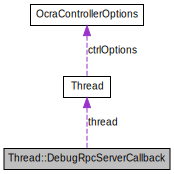
\includegraphics[width=246pt]{classThread_1_1DebugRpcServerCallback__coll__graph}
\end{center}
\end{figure}
\subsection*{\-Public \-Member \-Functions}
\begin{DoxyCompactItemize}
\item 
\hyperlink{classThread_1_1DebugRpcServerCallback_a479142cdf2f840df23b4605a532aaddf}{\-Debug\-Rpc\-Server\-Callback} (\hyperlink{classThread}{\-Thread} \&thread\-Ref)
\item 
virtual bool \hyperlink{classThread_1_1DebugRpcServerCallback_a3b39ac9b379ce3212bb2b05a89fa6024}{read} (yarp\-::os\-::\-Connection\-Reader \&connection)
\end{DoxyCompactItemize}
\subsection*{\-Private \-Attributes}
\begin{DoxyCompactItemize}
\item 
\hyperlink{classThread}{\-Thread} \& \hyperlink{classThread_1_1DebugRpcServerCallback_ad75683fc200019e8f681ad441b6ce84b}{thread}
\end{DoxyCompactItemize}


\subsection{\-Detailed \-Description}
\-A callback function which binds the rpc server port opened in the contoller server module to the controller thread's parsing function. 

\subsection{\-Constructor \& \-Destructor \-Documentation}
\hypertarget{classThread_1_1DebugRpcServerCallback_a479142cdf2f840df23b4605a532aaddf}{\index{\-Thread\-::\-Debug\-Rpc\-Server\-Callback@{\-Thread\-::\-Debug\-Rpc\-Server\-Callback}!\-Debug\-Rpc\-Server\-Callback@{\-Debug\-Rpc\-Server\-Callback}}
\index{\-Debug\-Rpc\-Server\-Callback@{\-Debug\-Rpc\-Server\-Callback}!Thread::DebugRpcServerCallback@{\-Thread\-::\-Debug\-Rpc\-Server\-Callback}}
\subsubsection[{\-Debug\-Rpc\-Server\-Callback}]{\setlength{\rightskip}{0pt plus 5cm}{\bf \-Thread\-::\-Debug\-Rpc\-Server\-Callback\-::\-Debug\-Rpc\-Server\-Callback} (
\begin{DoxyParamCaption}
\item[{{\bf \-Thread} \&}]{thread\-Ref}
\end{DoxyParamCaption}
)}}\label{classThread_1_1DebugRpcServerCallback_a479142cdf2f840df23b4605a532aaddf}
\-Constructor 
\begin{DoxyParams}{\-Parameters}
{\em ct\-Thread\-Ptr} & \-A shared pointer to the control thread. \\
\hline
\end{DoxyParams}


\subsection{\-Member \-Function \-Documentation}
\hypertarget{classThread_1_1DebugRpcServerCallback_a3b39ac9b379ce3212bb2b05a89fa6024}{\index{\-Thread\-::\-Debug\-Rpc\-Server\-Callback@{\-Thread\-::\-Debug\-Rpc\-Server\-Callback}!read@{read}}
\index{read@{read}!Thread::DebugRpcServerCallback@{\-Thread\-::\-Debug\-Rpc\-Server\-Callback}}
\subsubsection[{read}]{\setlength{\rightskip}{0pt plus 5cm}bool {\bf \-Thread\-::\-Debug\-Rpc\-Server\-Callback\-::read} (
\begin{DoxyParamCaption}
\item[{yarp\-::os\-::\-Connection\-Reader \&}]{connection}
\end{DoxyParamCaption}
)\hspace{0.3cm}{\ttfamily  \mbox{[}virtual\mbox{]}}}}\label{classThread_1_1DebugRpcServerCallback_a3b39ac9b379ce3212bb2b05a89fa6024}
read 
\begin{DoxyParams}{\-Parameters}
{\em connection} & \-Reads a port connection.\\
\hline
\end{DoxyParams}
\begin{DoxyReturn}{\-Returns}
\-A boolean which tells whether or not a message was read. 
\end{DoxyReturn}


\subsection{\-Member \-Data \-Documentation}
\hypertarget{classThread_1_1DebugRpcServerCallback_ad75683fc200019e8f681ad441b6ce84b}{\index{\-Thread\-::\-Debug\-Rpc\-Server\-Callback@{\-Thread\-::\-Debug\-Rpc\-Server\-Callback}!thread@{thread}}
\index{thread@{thread}!Thread::DebugRpcServerCallback@{\-Thread\-::\-Debug\-Rpc\-Server\-Callback}}
\subsubsection[{thread}]{\setlength{\rightskip}{0pt plus 5cm}{\bf \-Thread}\& {\bf \-Thread\-::\-Debug\-Rpc\-Server\-Callback\-::thread}\hspace{0.3cm}{\ttfamily  \mbox{[}private\mbox{]}}}}\label{classThread_1_1DebugRpcServerCallback_ad75683fc200019e8f681ad441b6ce84b}
\-A shared pointer to the control thread. 

\-The documentation for this class was generated from the following files\-:\begin{DoxyCompactItemize}
\item 
ocra-\/wbi-\/plugins/ocra-\/icub-\/server/include/ocra-\/icub-\/server/\hyperlink{Thread_8h}{\-Thread.\-h}\item 
ocra-\/wbi-\/plugins/ocra-\/icub-\/server/src/\hyperlink{Thread_8cpp}{\-Thread.\-cpp}\end{DoxyCompactItemize}

\hypertarget{classExampleClient}{\section{\-Example\-Client \-Class \-Reference}
\label{classExampleClient}\index{\-Example\-Client@{\-Example\-Client}}
}


{\ttfamily \#include $<$\-Example\-Client.\-h$>$}

\subsection*{\-Public \-Member \-Functions}
\begin{DoxyCompactItemize}
\item 
\hyperlink{classExampleClient_aed7d851662cba1484ecf1db8161d6e62}{\-Example\-Client} (std\-::shared\-\_\-ptr$<$ ocra\-::\-Model $>$ model\-Ptr, const int loop\-Period)
\item 
virtual \hyperlink{classExampleClient_abdca7dbe5fdab81d7d661a677e5ccd14}{$\sim$\-Example\-Client} ()
\end{DoxyCompactItemize}
\subsection*{\-Protected \-Member \-Functions}
\begin{DoxyCompactItemize}
\item 
virtual bool \hyperlink{classExampleClient_ad504d1d87997fc95bfeca6aa925a4fa6}{initialize} ()
\item 
virtual void \hyperlink{classExampleClient_a5acf25784c1c5b51c2c085327f195002}{release} ()
\item 
virtual void \hyperlink{classExampleClient_afb58f3425aafe2d4c38195cb3c667dbc}{loop} ()
\end{DoxyCompactItemize}
\subsection*{\-Private \-Attributes}
\begin{DoxyCompactItemize}
\item 
double \hyperlink{classExampleClient_aaa5ec782e9aaa1e94d7182872f743c02}{start\-Time}
\item 
double \hyperlink{classExampleClient_acade7035d4e39290cbda08b98249a629}{wait\-Time}
\item 
bool \hyperlink{classExampleClient_a90ce0c4d970c903b3e6afb6f5ca2a228}{trigger}
\item 
bool \hyperlink{classExampleClient_acd2cf0f0479ff8bbf5b64924d83beb60}{done}
\item 
\-Eigen\-::\-Matrix\-Xd \hyperlink{classExampleClient_acf4657277ecb08168d9a17c208814823}{waypoints}
\item 
std\-::shared\-\_\-ptr\*
$<$ ocra\-\_\-recipes\-::\-Trajectory\-Thread $>$ \hyperlink{classExampleClient_a4311b0e8c4878c23df2b5ba048d8bc05}{left\-Hand\-Traj\-Thread}
\item 
bool \hyperlink{classExampleClient_a7fb2b50cbdac0ec3a32e44b5bbc3b11f}{p1}
\item 
bool \hyperlink{classExampleClient_a07c2bc5c5c522e77a726017c28db2ec9}{p2}
\item 
bool \hyperlink{classExampleClient_ab41df6f34a51e649051adbac6d3077f9}{p3}
\end{DoxyCompactItemize}


\subsection{\-Constructor \& \-Destructor \-Documentation}
\hypertarget{classExampleClient_aed7d851662cba1484ecf1db8161d6e62}{\index{\-Example\-Client@{\-Example\-Client}!\-Example\-Client@{\-Example\-Client}}
\index{\-Example\-Client@{\-Example\-Client}!ExampleClient@{\-Example\-Client}}
\subsubsection[{\-Example\-Client}]{\setlength{\rightskip}{0pt plus 5cm}{\bf \-Example\-Client\-::\-Example\-Client} (
\begin{DoxyParamCaption}
\item[{std\-::shared\-\_\-ptr$<$ ocra\-::\-Model $>$}]{model\-Ptr, }
\item[{const int}]{loop\-Period}
\end{DoxyParamCaption}
)}}\label{classExampleClient_aed7d851662cba1484ecf1db8161d6e62}
\hypertarget{classExampleClient_abdca7dbe5fdab81d7d661a677e5ccd14}{\index{\-Example\-Client@{\-Example\-Client}!$\sim$\-Example\-Client@{$\sim$\-Example\-Client}}
\index{$\sim$\-Example\-Client@{$\sim$\-Example\-Client}!ExampleClient@{\-Example\-Client}}
\subsubsection[{$\sim$\-Example\-Client}]{\setlength{\rightskip}{0pt plus 5cm}{\bf \-Example\-Client\-::$\sim$\-Example\-Client} (
\begin{DoxyParamCaption}
{}
\end{DoxyParamCaption}
)\hspace{0.3cm}{\ttfamily  \mbox{[}virtual\mbox{]}}}}\label{classExampleClient_abdca7dbe5fdab81d7d661a677e5ccd14}


\subsection{\-Member \-Function \-Documentation}
\hypertarget{classExampleClient_ad504d1d87997fc95bfeca6aa925a4fa6}{\index{\-Example\-Client@{\-Example\-Client}!initialize@{initialize}}
\index{initialize@{initialize}!ExampleClient@{\-Example\-Client}}
\subsubsection[{initialize}]{\setlength{\rightskip}{0pt plus 5cm}bool {\bf \-Example\-Client\-::initialize} (
\begin{DoxyParamCaption}
{}
\end{DoxyParamCaption}
)\hspace{0.3cm}{\ttfamily  \mbox{[}protected, virtual\mbox{]}}}}\label{classExampleClient_ad504d1d87997fc95bfeca6aa925a4fa6}
\hypertarget{classExampleClient_afb58f3425aafe2d4c38195cb3c667dbc}{\index{\-Example\-Client@{\-Example\-Client}!loop@{loop}}
\index{loop@{loop}!ExampleClient@{\-Example\-Client}}
\subsubsection[{loop}]{\setlength{\rightskip}{0pt plus 5cm}void {\bf \-Example\-Client\-::loop} (
\begin{DoxyParamCaption}
{}
\end{DoxyParamCaption}
)\hspace{0.3cm}{\ttfamily  \mbox{[}protected, virtual\mbox{]}}}}\label{classExampleClient_afb58f3425aafe2d4c38195cb3c667dbc}
\hypertarget{classExampleClient_a5acf25784c1c5b51c2c085327f195002}{\index{\-Example\-Client@{\-Example\-Client}!release@{release}}
\index{release@{release}!ExampleClient@{\-Example\-Client}}
\subsubsection[{release}]{\setlength{\rightskip}{0pt plus 5cm}void {\bf \-Example\-Client\-::release} (
\begin{DoxyParamCaption}
{}
\end{DoxyParamCaption}
)\hspace{0.3cm}{\ttfamily  \mbox{[}protected, virtual\mbox{]}}}}\label{classExampleClient_a5acf25784c1c5b51c2c085327f195002}


\subsection{\-Member \-Data \-Documentation}
\hypertarget{classExampleClient_acd2cf0f0479ff8bbf5b64924d83beb60}{\index{\-Example\-Client@{\-Example\-Client}!done@{done}}
\index{done@{done}!ExampleClient@{\-Example\-Client}}
\subsubsection[{done}]{\setlength{\rightskip}{0pt plus 5cm}bool {\bf \-Example\-Client\-::done}\hspace{0.3cm}{\ttfamily  \mbox{[}private\mbox{]}}}}\label{classExampleClient_acd2cf0f0479ff8bbf5b64924d83beb60}
\hypertarget{classExampleClient_a4311b0e8c4878c23df2b5ba048d8bc05}{\index{\-Example\-Client@{\-Example\-Client}!left\-Hand\-Traj\-Thread@{left\-Hand\-Traj\-Thread}}
\index{left\-Hand\-Traj\-Thread@{left\-Hand\-Traj\-Thread}!ExampleClient@{\-Example\-Client}}
\subsubsection[{left\-Hand\-Traj\-Thread}]{\setlength{\rightskip}{0pt plus 5cm}std\-::shared\-\_\-ptr$<$ocra\-\_\-recipes\-::\-Trajectory\-Thread$>$ {\bf \-Example\-Client\-::left\-Hand\-Traj\-Thread}\hspace{0.3cm}{\ttfamily  \mbox{[}private\mbox{]}}}}\label{classExampleClient_a4311b0e8c4878c23df2b5ba048d8bc05}
\hypertarget{classExampleClient_a7fb2b50cbdac0ec3a32e44b5bbc3b11f}{\index{\-Example\-Client@{\-Example\-Client}!p1@{p1}}
\index{p1@{p1}!ExampleClient@{\-Example\-Client}}
\subsubsection[{p1}]{\setlength{\rightskip}{0pt plus 5cm}bool {\bf \-Example\-Client\-::p1}\hspace{0.3cm}{\ttfamily  \mbox{[}private\mbox{]}}}}\label{classExampleClient_a7fb2b50cbdac0ec3a32e44b5bbc3b11f}
\hypertarget{classExampleClient_a07c2bc5c5c522e77a726017c28db2ec9}{\index{\-Example\-Client@{\-Example\-Client}!p2@{p2}}
\index{p2@{p2}!ExampleClient@{\-Example\-Client}}
\subsubsection[{p2}]{\setlength{\rightskip}{0pt plus 5cm}bool {\bf \-Example\-Client\-::p2}\hspace{0.3cm}{\ttfamily  \mbox{[}private\mbox{]}}}}\label{classExampleClient_a07c2bc5c5c522e77a726017c28db2ec9}
\hypertarget{classExampleClient_ab41df6f34a51e649051adbac6d3077f9}{\index{\-Example\-Client@{\-Example\-Client}!p3@{p3}}
\index{p3@{p3}!ExampleClient@{\-Example\-Client}}
\subsubsection[{p3}]{\setlength{\rightskip}{0pt plus 5cm}bool {\bf \-Example\-Client\-::p3}\hspace{0.3cm}{\ttfamily  \mbox{[}private\mbox{]}}}}\label{classExampleClient_ab41df6f34a51e649051adbac6d3077f9}
\hypertarget{classExampleClient_aaa5ec782e9aaa1e94d7182872f743c02}{\index{\-Example\-Client@{\-Example\-Client}!start\-Time@{start\-Time}}
\index{start\-Time@{start\-Time}!ExampleClient@{\-Example\-Client}}
\subsubsection[{start\-Time}]{\setlength{\rightskip}{0pt plus 5cm}double {\bf \-Example\-Client\-::start\-Time}\hspace{0.3cm}{\ttfamily  \mbox{[}private\mbox{]}}}}\label{classExampleClient_aaa5ec782e9aaa1e94d7182872f743c02}
\hypertarget{classExampleClient_a90ce0c4d970c903b3e6afb6f5ca2a228}{\index{\-Example\-Client@{\-Example\-Client}!trigger@{trigger}}
\index{trigger@{trigger}!ExampleClient@{\-Example\-Client}}
\subsubsection[{trigger}]{\setlength{\rightskip}{0pt plus 5cm}bool {\bf \-Example\-Client\-::trigger}\hspace{0.3cm}{\ttfamily  \mbox{[}private\mbox{]}}}}\label{classExampleClient_a90ce0c4d970c903b3e6afb6f5ca2a228}
\hypertarget{classExampleClient_acade7035d4e39290cbda08b98249a629}{\index{\-Example\-Client@{\-Example\-Client}!wait\-Time@{wait\-Time}}
\index{wait\-Time@{wait\-Time}!ExampleClient@{\-Example\-Client}}
\subsubsection[{wait\-Time}]{\setlength{\rightskip}{0pt plus 5cm}double {\bf \-Example\-Client\-::wait\-Time}\hspace{0.3cm}{\ttfamily  \mbox{[}private\mbox{]}}}}\label{classExampleClient_acade7035d4e39290cbda08b98249a629}
\hypertarget{classExampleClient_acf4657277ecb08168d9a17c208814823}{\index{\-Example\-Client@{\-Example\-Client}!waypoints@{waypoints}}
\index{waypoints@{waypoints}!ExampleClient@{\-Example\-Client}}
\subsubsection[{waypoints}]{\setlength{\rightskip}{0pt plus 5cm}\-Eigen\-::\-Matrix\-Xd {\bf \-Example\-Client\-::waypoints}\hspace{0.3cm}{\ttfamily  \mbox{[}private\mbox{]}}}}\label{classExampleClient_acf4657277ecb08168d9a17c208814823}


\-The documentation for this class was generated from the following files\-:\begin{DoxyCompactItemize}
\item 
ocra-\/wbi-\/plugins/ocra-\/icub-\/clients/example-\/client/include/example-\/client/\hyperlink{ExampleClient_8h}{\-Example\-Client.\-h}\item 
ocra-\/wbi-\/plugins/ocra-\/icub-\/clients/example-\/client/src/\hyperlink{ExampleClient_8cpp}{\-Example\-Client.\-cpp}\end{DoxyCompactItemize}

\hypertarget{classIcubControllerServer}{\section{\-Icub\-Controller\-Server \-Class \-Reference}
\label{classIcubControllerServer}\index{\-Icub\-Controller\-Server@{\-Icub\-Controller\-Server}}
}


{\ttfamily \#include $<$\-Icub\-Controller\-Server.\-h$>$}

\subsection*{\-Public \-Member \-Functions}
\begin{DoxyCompactItemize}
\item 
\hyperlink{classIcubControllerServer_a6b0a6021e3c82e72ac97ad30d3f0c082}{\-Icub\-Controller\-Server} (std\-::shared\-\_\-ptr$<$ wbi\-::whole\-Body\-Interface $>$ robot, std\-::string icub\-Name, const bool using\-Floating\-Base, const ocra\-\_\-recipes\-::\-C\-O\-N\-T\-R\-O\-L\-L\-E\-R\-\_\-\-T\-Y\-P\-E ctrl\-Type=ocra\-\_\-recipes\-::\-W\-O\-C\-R\-A\-\_\-\-C\-O\-N\-T\-R\-O\-L\-L\-E\-R, const ocra\-\_\-recipes\-::\-S\-O\-L\-V\-E\-R\-\_\-\-T\-Y\-P\-E solver=ocra\-\_\-recipes\-::\-Q\-U\-A\-D\-P\-R\-O\-G, const bool using\-Interprocess\-Communication=true, const bool \hyperlink{classIcubControllerServer_adc410f503b14ed288c01e877ac405114}{use\-Odometry}=false)
\item 
virtual \hyperlink{classIcubControllerServer_a7582d4bbf9851ee9b58913ea2a89e5fd}{$\sim$\-Icub\-Controller\-Server} ()
\item 
virtual ocra\-::\-Model\-::\-Ptr \hyperlink{classIcubControllerServer_a025d8e257a69ef3d2c5a10b3cbfe2350}{load\-Robot\-Model} ()
\item 
virtual void \hyperlink{classIcubControllerServer_ac068c7930f342bb0cb0969d0d04267cf}{get\-Robot\-State} (\-Eigen\-::\-Vector\-Xd \&q, \-Eigen\-::\-Vector\-Xd \&qd, \-Eigen\-::\-Displacementd \&\-H\-\_\-root, \-Eigen\-::\-Twistd \&\-T\-\_\-root)
\item 
bool \hyperlink{classIcubControllerServer_a810f139a27e06458549ccbb3fde12359}{initialize\-Odometry} (std\-::string model\-\_\-file, std\-::string initial\-Fixed\-Frame)
\item 
std\-::vector$<$ std\-::string $>$ \hyperlink{classIcubControllerServer_a892bb43e568d3f112465dff1e0c6b348}{get\-Canonical\-\_\-i\-Cub\-Joints} ()
\item 
void \hyperlink{classIcubControllerServer_a032c035880f8ec2b77ef14521be6e75a}{root\-Frame\-Velocity} (\-Eigen\-::\-Vector\-Xd \&q, \-Eigen\-::\-Vector\-Xd \&qd, i\-Dyn\-Tree\-::\-Transform \&wbi\-\_\-\-H\-\_\-root\-\_\-\-Transform, double regularization, int \-L\-E\-F\-T\-\_\-\-F\-O\-O\-T\-\_\-\-C\-O\-N\-T\-A\-C\-T, int \-R\-I\-G\-H\-T\-\_\-\-F\-O\-O\-T\-\_\-\-C\-O\-N\-T\-A\-C\-T, \-Eigen\-::\-Vector\-Xd \&twist)
\item 
void \hyperlink{classIcubControllerServer_a27211ecba9fc8618733bcaea9ff7d140}{root\-Frame\-Velocity\-Piv\-L\-U} (\-Eigen\-::\-Vector\-Xd \&q, \-Eigen\-::\-Vector\-Xd \&qd, i\-Dyn\-Tree\-::\-Transform \&wbi\-\_\-\-H\-\_\-root\-\_\-\-Transform, \-Eigen\-::\-Vector\-Xd \&twist)
\item 
void \hyperlink{classIcubControllerServer_a82650f373c3c2c52a91cc744c67b0dcf}{root\-Frame\-Velocity\-Piv\-L\-U} (\-Eigen\-::\-Vector\-Xd \&q, \-Eigen\-::\-Vector\-Xd \&qd, i\-Dyn\-Tree\-::\-Transform \&wbi\-\_\-\-H\-\_\-root\-\_\-\-Transform, int \-L\-E\-F\-T\-\_\-\-F\-O\-O\-T\-\_\-\-C\-O\-N\-T\-A\-C\-T, int \-R\-I\-G\-H\-T\-\_\-\-F\-O\-O\-T\-\_\-\-C\-O\-N\-T\-A\-C\-T, \-Eigen\-::\-Vector\-Xd \&twist)
\item 
void \hyperlink{classIcubControllerServer_a0132b1ddc3dafd29506e4684ea42cf58}{pinv} (\-Eigen\-::\-Matrix\-Xd mat, \-Eigen\-::\-Matrix\-Xd \&pinvmat, double pinvtoler=1.\-0e-\/6) const 
\item 
void \hyperlink{classIcubControllerServer_aaedff28c5d9ac9a7cdbc24c9e0cbc5b3}{velocity\-Error} (\-Eigen\-::\-Matrix\-Xd \-A, \-Eigen\-::\-Matrix\-Xd \-B, \-Eigen\-::\-Matrix\-Xd \-X)
\end{DoxyCompactItemize}
\subsection*{\-Private \-Attributes}
\begin{DoxyCompactItemize}
\item 
std\-::shared\-\_\-ptr\*
$<$ wbi\-::whole\-Body\-Interface $>$ \hyperlink{classIcubControllerServer_ae8a89707675adb58bb3006bc085828b7}{wbi}
\item 
std\-::string \hyperlink{classIcubControllerServer_a041d6687258c36677914b1d15f18e153}{robot\-Name}
\item 
bool \hyperlink{classIcubControllerServer_aebc2019921c3eabb53c01012fbd2355a}{is\-Floating\-Base}
\item 
bool \hyperlink{classIcubControllerServer_adc410f503b14ed288c01e877ac405114}{use\-Odometry}
\item 
int \hyperlink{classIcubControllerServer_ab5fb1f18775cfe3036894c73dc21ebcf}{n\-Do\-F}
\item 
\-Eigen\-::\-Vector\-Xd \hyperlink{classIcubControllerServer_a42f6a8db660da9dbafbc57941b1ee12f}{wbi\-\_\-\-H\-\_\-root\-\_\-\-Vector}
\item 
\-Eigen\-::\-Vector\-Xd \hyperlink{classIcubControllerServer_a818b66e75b7f9457a6a5bcbb3c1306a7}{wbi\-\_\-\-T\-\_\-root\-\_\-\-Vector}
\item 
wbi\-::\-Frame \hyperlink{classIcubControllerServer_afd983b69c043eedf958e53582b22195a}{wbi\-\_\-\-H\-\_\-root}
\item 
i\-Dyn\-Tree\-::\-Simple\-Legged\-Odometry \hyperlink{classIcubControllerServer_ad0484106ab9d7fd42e2bd682338871c7}{odometry}
\end{DoxyCompactItemize}
\subsection*{\-Static \-Private \-Attributes}
\begin{DoxyCompactItemize}
\item 
static constexpr double \hyperlink{classIcubControllerServer_a8d077d5e0d0fe0107e6f4f151bd03f2c}{\-A\-L\-L\-\_\-\-J\-O\-I\-N\-T\-S} = -\/1.\-0
\end{DoxyCompactItemize}


\subsection{\-Constructor \& \-Destructor \-Documentation}
\hypertarget{classIcubControllerServer_a6b0a6021e3c82e72ac97ad30d3f0c082}{\index{\-Icub\-Controller\-Server@{\-Icub\-Controller\-Server}!\-Icub\-Controller\-Server@{\-Icub\-Controller\-Server}}
\index{\-Icub\-Controller\-Server@{\-Icub\-Controller\-Server}!IcubControllerServer@{\-Icub\-Controller\-Server}}
\subsubsection[{\-Icub\-Controller\-Server}]{\setlength{\rightskip}{0pt plus 5cm}{\bf \-Icub\-Controller\-Server\-::\-Icub\-Controller\-Server} (
\begin{DoxyParamCaption}
\item[{std\-::shared\-\_\-ptr$<$ wbi\-::whole\-Body\-Interface $>$}]{robot, }
\item[{std\-::string}]{icub\-Name, }
\item[{const bool}]{using\-Floating\-Base, }
\item[{const ocra\-\_\-recipes\-::\-C\-O\-N\-T\-R\-O\-L\-L\-E\-R\-\_\-\-T\-Y\-P\-E}]{ctrl\-Type = {\ttfamily ocra\-\_\-recipes\-:\-:\-W\-O\-C\-R\-A\-\_\-\-C\-O\-N\-T\-R\-O\-L\-L\-E\-R}, }
\item[{const ocra\-\_\-recipes\-::\-S\-O\-L\-V\-E\-R\-\_\-\-T\-Y\-P\-E}]{solver = {\ttfamily ocra\-\_\-recipes\-:\-:\-Q\-U\-A\-D\-P\-R\-O\-G}, }
\item[{const bool}]{using\-Interprocess\-Communication = {\ttfamily true}, }
\item[{const bool}]{use\-Odometry = {\ttfamily false}}
\end{DoxyParamCaption}
)}}\label{classIcubControllerServer_a6b0a6021e3c82e72ac97ad30d3f0c082}
\hypertarget{classIcubControllerServer_a7582d4bbf9851ee9b58913ea2a89e5fd}{\index{\-Icub\-Controller\-Server@{\-Icub\-Controller\-Server}!$\sim$\-Icub\-Controller\-Server@{$\sim$\-Icub\-Controller\-Server}}
\index{$\sim$\-Icub\-Controller\-Server@{$\sim$\-Icub\-Controller\-Server}!IcubControllerServer@{\-Icub\-Controller\-Server}}
\subsubsection[{$\sim$\-Icub\-Controller\-Server}]{\setlength{\rightskip}{0pt plus 5cm}{\bf \-Icub\-Controller\-Server\-::$\sim$\-Icub\-Controller\-Server} (
\begin{DoxyParamCaption}
{}
\end{DoxyParamCaption}
)\hspace{0.3cm}{\ttfamily  \mbox{[}virtual\mbox{]}}}}\label{classIcubControllerServer_a7582d4bbf9851ee9b58913ea2a89e5fd}


\subsection{\-Member \-Function \-Documentation}
\hypertarget{classIcubControllerServer_a892bb43e568d3f112465dff1e0c6b348}{\index{\-Icub\-Controller\-Server@{\-Icub\-Controller\-Server}!get\-Canonical\-\_\-i\-Cub\-Joints@{get\-Canonical\-\_\-i\-Cub\-Joints}}
\index{get\-Canonical\-\_\-i\-Cub\-Joints@{get\-Canonical\-\_\-i\-Cub\-Joints}!IcubControllerServer@{\-Icub\-Controller\-Server}}
\subsubsection[{get\-Canonical\-\_\-i\-Cub\-Joints}]{\setlength{\rightskip}{0pt plus 5cm}std\-::vector$<$ std\-::string $>$ {\bf \-Icub\-Controller\-Server\-::get\-Canonical\-\_\-i\-Cub\-Joints} (
\begin{DoxyParamCaption}
{}
\end{DoxyParamCaption}
)}}\label{classIcubControllerServer_a892bb43e568d3f112465dff1e0c6b348}
\hypertarget{classIcubControllerServer_ac068c7930f342bb0cb0969d0d04267cf}{\index{\-Icub\-Controller\-Server@{\-Icub\-Controller\-Server}!get\-Robot\-State@{get\-Robot\-State}}
\index{get\-Robot\-State@{get\-Robot\-State}!IcubControllerServer@{\-Icub\-Controller\-Server}}
\subsubsection[{get\-Robot\-State}]{\setlength{\rightskip}{0pt plus 5cm}void {\bf \-Icub\-Controller\-Server\-::get\-Robot\-State} (
\begin{DoxyParamCaption}
\item[{\-Eigen\-::\-Vector\-Xd \&}]{q, }
\item[{\-Eigen\-::\-Vector\-Xd \&}]{qd, }
\item[{\-Eigen\-::\-Displacementd \&}]{\-H\-\_\-root, }
\item[{\-Eigen\-::\-Twistd \&}]{\-T\-\_\-root}
\end{DoxyParamCaption}
)\hspace{0.3cm}{\ttfamily  \mbox{[}virtual\mbox{]}}}}\label{classIcubControllerServer_ac068c7930f342bb0cb0969d0d04267cf}
\hypertarget{classIcubControllerServer_a810f139a27e06458549ccbb3fde12359}{\index{\-Icub\-Controller\-Server@{\-Icub\-Controller\-Server}!initialize\-Odometry@{initialize\-Odometry}}
\index{initialize\-Odometry@{initialize\-Odometry}!IcubControllerServer@{\-Icub\-Controller\-Server}}
\subsubsection[{initialize\-Odometry}]{\setlength{\rightskip}{0pt plus 5cm}bool {\bf \-Icub\-Controller\-Server\-::initialize\-Odometry} (
\begin{DoxyParamCaption}
\item[{std\-::string}]{model\-\_\-file, }
\item[{std\-::string}]{initial\-Fixed\-Frame}
\end{DoxyParamCaption}
)}}\label{classIcubControllerServer_a810f139a27e06458549ccbb3fde12359}
\hypertarget{classIcubControllerServer_a025d8e257a69ef3d2c5a10b3cbfe2350}{\index{\-Icub\-Controller\-Server@{\-Icub\-Controller\-Server}!load\-Robot\-Model@{load\-Robot\-Model}}
\index{load\-Robot\-Model@{load\-Robot\-Model}!IcubControllerServer@{\-Icub\-Controller\-Server}}
\subsubsection[{load\-Robot\-Model}]{\setlength{\rightskip}{0pt plus 5cm}ocra\-::\-Model\-::\-Ptr {\bf \-Icub\-Controller\-Server\-::load\-Robot\-Model} (
\begin{DoxyParamCaption}
{}
\end{DoxyParamCaption}
)\hspace{0.3cm}{\ttfamily  \mbox{[}virtual\mbox{]}}}}\label{classIcubControllerServer_a025d8e257a69ef3d2c5a10b3cbfe2350}
\hypertarget{classIcubControllerServer_a0132b1ddc3dafd29506e4684ea42cf58}{\index{\-Icub\-Controller\-Server@{\-Icub\-Controller\-Server}!pinv@{pinv}}
\index{pinv@{pinv}!IcubControllerServer@{\-Icub\-Controller\-Server}}
\subsubsection[{pinv}]{\setlength{\rightskip}{0pt plus 5cm}void {\bf \-Icub\-Controller\-Server\-::pinv} (
\begin{DoxyParamCaption}
\item[{\-Eigen\-::\-Matrix\-Xd}]{mat, }
\item[{\-Eigen\-::\-Matrix\-Xd \&}]{pinvmat, }
\item[{double}]{pinvtoler = {\ttfamily 1.0e-\/6}}
\end{DoxyParamCaption}
) const}}\label{classIcubControllerServer_a0132b1ddc3dafd29506e4684ea42cf58}
\hypertarget{classIcubControllerServer_a032c035880f8ec2b77ef14521be6e75a}{\index{\-Icub\-Controller\-Server@{\-Icub\-Controller\-Server}!root\-Frame\-Velocity@{root\-Frame\-Velocity}}
\index{root\-Frame\-Velocity@{root\-Frame\-Velocity}!IcubControllerServer@{\-Icub\-Controller\-Server}}
\subsubsection[{root\-Frame\-Velocity}]{\setlength{\rightskip}{0pt plus 5cm}void {\bf \-Icub\-Controller\-Server\-::root\-Frame\-Velocity} (
\begin{DoxyParamCaption}
\item[{\-Eigen\-::\-Vector\-Xd \&}]{q, }
\item[{\-Eigen\-::\-Vector\-Xd \&}]{qd, }
\item[{i\-Dyn\-Tree\-::\-Transform \&}]{wbi\-\_\-\-H\-\_\-root\-\_\-\-Transform, }
\item[{double}]{regularization, }
\item[{int}]{\-L\-E\-F\-T\-\_\-\-F\-O\-O\-T\-\_\-\-C\-O\-N\-T\-A\-C\-T, }
\item[{int}]{\-R\-I\-G\-H\-T\-\_\-\-F\-O\-O\-T\-\_\-\-C\-O\-N\-T\-A\-C\-T, }
\item[{\-Eigen\-::\-Vector\-Xd \&}]{twist}
\end{DoxyParamCaption}
)}}\label{classIcubControllerServer_a032c035880f8ec2b77ef14521be6e75a}
\hypertarget{classIcubControllerServer_a27211ecba9fc8618733bcaea9ff7d140}{\index{\-Icub\-Controller\-Server@{\-Icub\-Controller\-Server}!root\-Frame\-Velocity\-Piv\-L\-U@{root\-Frame\-Velocity\-Piv\-L\-U}}
\index{root\-Frame\-Velocity\-Piv\-L\-U@{root\-Frame\-Velocity\-Piv\-L\-U}!IcubControllerServer@{\-Icub\-Controller\-Server}}
\subsubsection[{root\-Frame\-Velocity\-Piv\-L\-U}]{\setlength{\rightskip}{0pt plus 5cm}void {\bf \-Icub\-Controller\-Server\-::root\-Frame\-Velocity\-Piv\-L\-U} (
\begin{DoxyParamCaption}
\item[{\-Eigen\-::\-Vector\-Xd \&}]{q, }
\item[{\-Eigen\-::\-Vector\-Xd \&}]{qd, }
\item[{i\-Dyn\-Tree\-::\-Transform \&}]{wbi\-\_\-\-H\-\_\-root\-\_\-\-Transform, }
\item[{\-Eigen\-::\-Vector\-Xd \&}]{twist}
\end{DoxyParamCaption}
)}}\label{classIcubControllerServer_a27211ecba9fc8618733bcaea9ff7d140}
\hypertarget{classIcubControllerServer_a82650f373c3c2c52a91cc744c67b0dcf}{\index{\-Icub\-Controller\-Server@{\-Icub\-Controller\-Server}!root\-Frame\-Velocity\-Piv\-L\-U@{root\-Frame\-Velocity\-Piv\-L\-U}}
\index{root\-Frame\-Velocity\-Piv\-L\-U@{root\-Frame\-Velocity\-Piv\-L\-U}!IcubControllerServer@{\-Icub\-Controller\-Server}}
\subsubsection[{root\-Frame\-Velocity\-Piv\-L\-U}]{\setlength{\rightskip}{0pt plus 5cm}void {\bf \-Icub\-Controller\-Server\-::root\-Frame\-Velocity\-Piv\-L\-U} (
\begin{DoxyParamCaption}
\item[{\-Eigen\-::\-Vector\-Xd \&}]{q, }
\item[{\-Eigen\-::\-Vector\-Xd \&}]{qd, }
\item[{i\-Dyn\-Tree\-::\-Transform \&}]{wbi\-\_\-\-H\-\_\-root\-\_\-\-Transform, }
\item[{int}]{\-L\-E\-F\-T\-\_\-\-F\-O\-O\-T\-\_\-\-C\-O\-N\-T\-A\-C\-T, }
\item[{int}]{\-R\-I\-G\-H\-T\-\_\-\-F\-O\-O\-T\-\_\-\-C\-O\-N\-T\-A\-C\-T, }
\item[{\-Eigen\-::\-Vector\-Xd \&}]{twist}
\end{DoxyParamCaption}
)}}\label{classIcubControllerServer_a82650f373c3c2c52a91cc744c67b0dcf}
\hypertarget{classIcubControllerServer_aaedff28c5d9ac9a7cdbc24c9e0cbc5b3}{\index{\-Icub\-Controller\-Server@{\-Icub\-Controller\-Server}!velocity\-Error@{velocity\-Error}}
\index{velocity\-Error@{velocity\-Error}!IcubControllerServer@{\-Icub\-Controller\-Server}}
\subsubsection[{velocity\-Error}]{\setlength{\rightskip}{0pt plus 5cm}void {\bf \-Icub\-Controller\-Server\-::velocity\-Error} (
\begin{DoxyParamCaption}
\item[{\-Eigen\-::\-Matrix\-Xd}]{\-A, }
\item[{\-Eigen\-::\-Matrix\-Xd}]{\-B, }
\item[{\-Eigen\-::\-Matrix\-Xd}]{\-X}
\end{DoxyParamCaption}
)}}\label{classIcubControllerServer_aaedff28c5d9ac9a7cdbc24c9e0cbc5b3}


\subsection{\-Member \-Data \-Documentation}
\hypertarget{classIcubControllerServer_a8d077d5e0d0fe0107e6f4f151bd03f2c}{\index{\-Icub\-Controller\-Server@{\-Icub\-Controller\-Server}!\-A\-L\-L\-\_\-\-J\-O\-I\-N\-T\-S@{\-A\-L\-L\-\_\-\-J\-O\-I\-N\-T\-S}}
\index{\-A\-L\-L\-\_\-\-J\-O\-I\-N\-T\-S@{\-A\-L\-L\-\_\-\-J\-O\-I\-N\-T\-S}!IcubControllerServer@{\-Icub\-Controller\-Server}}
\subsubsection[{\-A\-L\-L\-\_\-\-J\-O\-I\-N\-T\-S}]{\setlength{\rightskip}{0pt plus 5cm}constexpr double {\bf \-Icub\-Controller\-Server\-::\-A\-L\-L\-\_\-\-J\-O\-I\-N\-T\-S} = -\/1.\-0\hspace{0.3cm}{\ttfamily  \mbox{[}static, private\mbox{]}}}}\label{classIcubControllerServer_a8d077d5e0d0fe0107e6f4f151bd03f2c}
\hypertarget{classIcubControllerServer_aebc2019921c3eabb53c01012fbd2355a}{\index{\-Icub\-Controller\-Server@{\-Icub\-Controller\-Server}!is\-Floating\-Base@{is\-Floating\-Base}}
\index{is\-Floating\-Base@{is\-Floating\-Base}!IcubControllerServer@{\-Icub\-Controller\-Server}}
\subsubsection[{is\-Floating\-Base}]{\setlength{\rightskip}{0pt plus 5cm}bool {\bf \-Icub\-Controller\-Server\-::is\-Floating\-Base}\hspace{0.3cm}{\ttfamily  \mbox{[}private\mbox{]}}}}\label{classIcubControllerServer_aebc2019921c3eabb53c01012fbd2355a}
\hypertarget{classIcubControllerServer_ab5fb1f18775cfe3036894c73dc21ebcf}{\index{\-Icub\-Controller\-Server@{\-Icub\-Controller\-Server}!n\-Do\-F@{n\-Do\-F}}
\index{n\-Do\-F@{n\-Do\-F}!IcubControllerServer@{\-Icub\-Controller\-Server}}
\subsubsection[{n\-Do\-F}]{\setlength{\rightskip}{0pt plus 5cm}int {\bf \-Icub\-Controller\-Server\-::n\-Do\-F}\hspace{0.3cm}{\ttfamily  \mbox{[}private\mbox{]}}}}\label{classIcubControllerServer_ab5fb1f18775cfe3036894c73dc21ebcf}
\hypertarget{classIcubControllerServer_ad0484106ab9d7fd42e2bd682338871c7}{\index{\-Icub\-Controller\-Server@{\-Icub\-Controller\-Server}!odometry@{odometry}}
\index{odometry@{odometry}!IcubControllerServer@{\-Icub\-Controller\-Server}}
\subsubsection[{odometry}]{\setlength{\rightskip}{0pt plus 5cm}i\-Dyn\-Tree\-::\-Simple\-Legged\-Odometry {\bf \-Icub\-Controller\-Server\-::odometry}\hspace{0.3cm}{\ttfamily  \mbox{[}private\mbox{]}}}}\label{classIcubControllerServer_ad0484106ab9d7fd42e2bd682338871c7}
\hypertarget{classIcubControllerServer_a041d6687258c36677914b1d15f18e153}{\index{\-Icub\-Controller\-Server@{\-Icub\-Controller\-Server}!robot\-Name@{robot\-Name}}
\index{robot\-Name@{robot\-Name}!IcubControllerServer@{\-Icub\-Controller\-Server}}
\subsubsection[{robot\-Name}]{\setlength{\rightskip}{0pt plus 5cm}std\-::string {\bf \-Icub\-Controller\-Server\-::robot\-Name}\hspace{0.3cm}{\ttfamily  \mbox{[}private\mbox{]}}}}\label{classIcubControllerServer_a041d6687258c36677914b1d15f18e153}
\hypertarget{classIcubControllerServer_adc410f503b14ed288c01e877ac405114}{\index{\-Icub\-Controller\-Server@{\-Icub\-Controller\-Server}!use\-Odometry@{use\-Odometry}}
\index{use\-Odometry@{use\-Odometry}!IcubControllerServer@{\-Icub\-Controller\-Server}}
\subsubsection[{use\-Odometry}]{\setlength{\rightskip}{0pt plus 5cm}bool {\bf \-Icub\-Controller\-Server\-::use\-Odometry}\hspace{0.3cm}{\ttfamily  \mbox{[}private\mbox{]}}}}\label{classIcubControllerServer_adc410f503b14ed288c01e877ac405114}
\hypertarget{classIcubControllerServer_ae8a89707675adb58bb3006bc085828b7}{\index{\-Icub\-Controller\-Server@{\-Icub\-Controller\-Server}!wbi@{wbi}}
\index{wbi@{wbi}!IcubControllerServer@{\-Icub\-Controller\-Server}}
\subsubsection[{wbi}]{\setlength{\rightskip}{0pt plus 5cm}std\-::shared\-\_\-ptr$<$wbi\-::whole\-Body\-Interface$>$ {\bf \-Icub\-Controller\-Server\-::wbi}\hspace{0.3cm}{\ttfamily  \mbox{[}private\mbox{]}}}}\label{classIcubControllerServer_ae8a89707675adb58bb3006bc085828b7}
\-The \-W\-B\-I used to talk to the robot. \hypertarget{classIcubControllerServer_afd983b69c043eedf958e53582b22195a}{\index{\-Icub\-Controller\-Server@{\-Icub\-Controller\-Server}!wbi\-\_\-\-H\-\_\-root@{wbi\-\_\-\-H\-\_\-root}}
\index{wbi\-\_\-\-H\-\_\-root@{wbi\-\_\-\-H\-\_\-root}!IcubControllerServer@{\-Icub\-Controller\-Server}}
\subsubsection[{wbi\-\_\-\-H\-\_\-root}]{\setlength{\rightskip}{0pt plus 5cm}wbi\-::\-Frame {\bf \-Icub\-Controller\-Server\-::wbi\-\_\-\-H\-\_\-root}\hspace{0.3cm}{\ttfamily  \mbox{[}private\mbox{]}}}}\label{classIcubControllerServer_afd983b69c043eedf958e53582b22195a}
\hypertarget{classIcubControllerServer_a42f6a8db660da9dbafbc57941b1ee12f}{\index{\-Icub\-Controller\-Server@{\-Icub\-Controller\-Server}!wbi\-\_\-\-H\-\_\-root\-\_\-\-Vector@{wbi\-\_\-\-H\-\_\-root\-\_\-\-Vector}}
\index{wbi\-\_\-\-H\-\_\-root\-\_\-\-Vector@{wbi\-\_\-\-H\-\_\-root\-\_\-\-Vector}!IcubControllerServer@{\-Icub\-Controller\-Server}}
\subsubsection[{wbi\-\_\-\-H\-\_\-root\-\_\-\-Vector}]{\setlength{\rightskip}{0pt plus 5cm}\-Eigen\-::\-Vector\-Xd {\bf \-Icub\-Controller\-Server\-::wbi\-\_\-\-H\-\_\-root\-\_\-\-Vector}\hspace{0.3cm}{\ttfamily  \mbox{[}private\mbox{]}}}}\label{classIcubControllerServer_a42f6a8db660da9dbafbc57941b1ee12f}
\hypertarget{classIcubControllerServer_a818b66e75b7f9457a6a5bcbb3c1306a7}{\index{\-Icub\-Controller\-Server@{\-Icub\-Controller\-Server}!wbi\-\_\-\-T\-\_\-root\-\_\-\-Vector@{wbi\-\_\-\-T\-\_\-root\-\_\-\-Vector}}
\index{wbi\-\_\-\-T\-\_\-root\-\_\-\-Vector@{wbi\-\_\-\-T\-\_\-root\-\_\-\-Vector}!IcubControllerServer@{\-Icub\-Controller\-Server}}
\subsubsection[{wbi\-\_\-\-T\-\_\-root\-\_\-\-Vector}]{\setlength{\rightskip}{0pt plus 5cm}\-Eigen\-::\-Vector\-Xd {\bf \-Icub\-Controller\-Server\-::wbi\-\_\-\-T\-\_\-root\-\_\-\-Vector}\hspace{0.3cm}{\ttfamily  \mbox{[}private\mbox{]}}}}\label{classIcubControllerServer_a818b66e75b7f9457a6a5bcbb3c1306a7}


\-The documentation for this class was generated from the following files\-:\begin{DoxyCompactItemize}
\item 
ocra-\/wbi-\/plugins/ocra-\/icub-\/server/include/ocra-\/icub-\/server/\hyperlink{IcubControllerServer_8h}{\-Icub\-Controller\-Server.\-h}\item 
ocra-\/wbi-\/plugins/ocra-\/icub-\/server/src/\hyperlink{IcubControllerServer_8cpp}{\-Icub\-Controller\-Server.\-cpp}\end{DoxyCompactItemize}

\hypertarget{classocra__icub_1_1ModelInitializer}{\section{ocra\-\_\-icub\-:\-:\-Model\-Initializer \-Class \-Reference}
\label{classocra__icub_1_1ModelInitializer}\index{ocra\-\_\-icub\-::\-Model\-Initializer@{ocra\-\_\-icub\-::\-Model\-Initializer}}
}


{\ttfamily \#include $<$\-Model\-Initializer.\-h$>$}

\subsection*{\-Public \-Member \-Functions}
\begin{DoxyCompactItemize}
\item 
\hyperlink{classocra__icub_1_1ModelInitializer_a14a314ebc05e38e472607b76951d31cc}{\-Model\-Initializer} ()
\item 
virtual \hyperlink{classocra__icub_1_1ModelInitializer_af72e47a78f20f34f77be2b9e6921ca19}{$\sim$\-Model\-Initializer} ()
\item 
std\-::shared\-\_\-ptr$<$ ocra\-::\-Model $>$ \hyperlink{classocra__icub_1_1ModelInitializer_aa8fbe9e7f20a2b4a29b6fce403c500c8}{get\-Model} ()
\end{DoxyCompactItemize}
\subsection*{\-Private \-Member \-Functions}
\begin{DoxyCompactItemize}
\item 
bool \hyperlink{classocra__icub_1_1ModelInitializer_afa7e888280149483f0ff27ced546801b}{configure\-Wbi} ()
\item 
void \hyperlink{classocra__icub_1_1ModelInitializer_a90747ff9773627f37ca9453491377b2c}{construct\-Model} ()
\item 
bool \hyperlink{classocra__icub_1_1ModelInitializer_abb762b28a1e7b57103f609c4fab4e94e}{get\-Configuration\-Info\-From\-Controller\-Server} ()
\item 
std\-::string \hyperlink{classocra__icub_1_1ModelInitializer_a086ea4822765ab6daff59fae1db0bd11}{get\-Unique\-Wbi\-Name} ()
\end{DoxyCompactItemize}
\subsection*{\-Private \-Attributes}
\begin{DoxyCompactItemize}
\item 
std\-::shared\-\_\-ptr\*
$<$ yarp\-Wbi\-::yarp\-Whole\-Body\-Interface $>$ \hyperlink{classocra__icub_1_1ModelInitializer_a86b4917ca6ebc3ec9239a4c417cb6b2a}{robot\-Interface}
\item 
std\-::shared\-\_\-ptr$<$ ocra\-::\-Model $>$ \hyperlink{classocra__icub_1_1ModelInitializer_ab7fb1fe2773837be8b3b41b75ef8f9d6}{model}
\item 
std\-::string \hyperlink{classocra__icub_1_1ModelInitializer_add617233dd3940f79f03cb6a2ed6adb5}{wbi\-Config\-File\-Path}
\item 
std\-::string \hyperlink{classocra__icub_1_1ModelInitializer_aef3121c44b93b22cf24c4ccbbc477128}{robot\-Name}
\item 
bool \hyperlink{classocra__icub_1_1ModelInitializer_a51d73f808c75fbc1284f460e7ff66d6a}{is\-Floating\-Base}
\item 
yarp\-::os\-::\-Log \hyperlink{classocra__icub_1_1ModelInitializer_a7ecf8156a05245831e51cc212eec5985}{y\-Log}
\item 
int \hyperlink{classocra__icub_1_1ModelInitializer_ab63cc70107cab38cc01a87d7a5465d85}{mod\-Init\-Number}
\end{DoxyCompactItemize}
\subsection*{\-Static \-Private \-Attributes}
\begin{DoxyCompactItemize}
\item 
static int \hyperlink{classocra__icub_1_1ModelInitializer_a8ec0a5af61b4a972ea22b71a5d3511eb}{\-M\-O\-D\-E\-L\-\_\-\-I\-N\-I\-T\-I\-A\-L\-I\-Z\-E\-R\-\_\-\-C\-O\-U\-N\-T} = 0
\end{DoxyCompactItemize}


\subsection{\-Constructor \& \-Destructor \-Documentation}
\hypertarget{classocra__icub_1_1ModelInitializer_a14a314ebc05e38e472607b76951d31cc}{\index{ocra\-\_\-icub\-::\-Model\-Initializer@{ocra\-\_\-icub\-::\-Model\-Initializer}!\-Model\-Initializer@{\-Model\-Initializer}}
\index{\-Model\-Initializer@{\-Model\-Initializer}!ocra_icub::ModelInitializer@{ocra\-\_\-icub\-::\-Model\-Initializer}}
\subsubsection[{\-Model\-Initializer}]{\setlength{\rightskip}{0pt plus 5cm}{\bf \-Model\-Initializer\-::\-Model\-Initializer} (
\begin{DoxyParamCaption}
{}
\end{DoxyParamCaption}
)}}\label{classocra__icub_1_1ModelInitializer_a14a314ebc05e38e472607b76951d31cc}
\hypertarget{classocra__icub_1_1ModelInitializer_af72e47a78f20f34f77be2b9e6921ca19}{\index{ocra\-\_\-icub\-::\-Model\-Initializer@{ocra\-\_\-icub\-::\-Model\-Initializer}!$\sim$\-Model\-Initializer@{$\sim$\-Model\-Initializer}}
\index{$\sim$\-Model\-Initializer@{$\sim$\-Model\-Initializer}!ocra_icub::ModelInitializer@{ocra\-\_\-icub\-::\-Model\-Initializer}}
\subsubsection[{$\sim$\-Model\-Initializer}]{\setlength{\rightskip}{0pt plus 5cm}{\bf \-Model\-Initializer\-::$\sim$\-Model\-Initializer} (
\begin{DoxyParamCaption}
{}
\end{DoxyParamCaption}
)\hspace{0.3cm}{\ttfamily  \mbox{[}virtual\mbox{]}}}}\label{classocra__icub_1_1ModelInitializer_af72e47a78f20f34f77be2b9e6921ca19}


\subsection{\-Member \-Function \-Documentation}
\hypertarget{classocra__icub_1_1ModelInitializer_afa7e888280149483f0ff27ced546801b}{\index{ocra\-\_\-icub\-::\-Model\-Initializer@{ocra\-\_\-icub\-::\-Model\-Initializer}!configure\-Wbi@{configure\-Wbi}}
\index{configure\-Wbi@{configure\-Wbi}!ocra_icub::ModelInitializer@{ocra\-\_\-icub\-::\-Model\-Initializer}}
\subsubsection[{configure\-Wbi}]{\setlength{\rightskip}{0pt plus 5cm}bool {\bf \-Model\-Initializer\-::configure\-Wbi} (
\begin{DoxyParamCaption}
{}
\end{DoxyParamCaption}
)\hspace{0.3cm}{\ttfamily  \mbox{[}private\mbox{]}}}}\label{classocra__icub_1_1ModelInitializer_afa7e888280149483f0ff27ced546801b}
\hypertarget{classocra__icub_1_1ModelInitializer_a90747ff9773627f37ca9453491377b2c}{\index{ocra\-\_\-icub\-::\-Model\-Initializer@{ocra\-\_\-icub\-::\-Model\-Initializer}!construct\-Model@{construct\-Model}}
\index{construct\-Model@{construct\-Model}!ocra_icub::ModelInitializer@{ocra\-\_\-icub\-::\-Model\-Initializer}}
\subsubsection[{construct\-Model}]{\setlength{\rightskip}{0pt plus 5cm}void {\bf \-Model\-Initializer\-::construct\-Model} (
\begin{DoxyParamCaption}
{}
\end{DoxyParamCaption}
)\hspace{0.3cm}{\ttfamily  \mbox{[}private\mbox{]}}}}\label{classocra__icub_1_1ModelInitializer_a90747ff9773627f37ca9453491377b2c}
\hypertarget{classocra__icub_1_1ModelInitializer_abb762b28a1e7b57103f609c4fab4e94e}{\index{ocra\-\_\-icub\-::\-Model\-Initializer@{ocra\-\_\-icub\-::\-Model\-Initializer}!get\-Configuration\-Info\-From\-Controller\-Server@{get\-Configuration\-Info\-From\-Controller\-Server}}
\index{get\-Configuration\-Info\-From\-Controller\-Server@{get\-Configuration\-Info\-From\-Controller\-Server}!ocra_icub::ModelInitializer@{ocra\-\_\-icub\-::\-Model\-Initializer}}
\subsubsection[{get\-Configuration\-Info\-From\-Controller\-Server}]{\setlength{\rightskip}{0pt plus 5cm}bool {\bf \-Model\-Initializer\-::get\-Configuration\-Info\-From\-Controller\-Server} (
\begin{DoxyParamCaption}
{}
\end{DoxyParamCaption}
)\hspace{0.3cm}{\ttfamily  \mbox{[}private\mbox{]}}}}\label{classocra__icub_1_1ModelInitializer_abb762b28a1e7b57103f609c4fab4e94e}
\hypertarget{classocra__icub_1_1ModelInitializer_aa8fbe9e7f20a2b4a29b6fce403c500c8}{\index{ocra\-\_\-icub\-::\-Model\-Initializer@{ocra\-\_\-icub\-::\-Model\-Initializer}!get\-Model@{get\-Model}}
\index{get\-Model@{get\-Model}!ocra_icub::ModelInitializer@{ocra\-\_\-icub\-::\-Model\-Initializer}}
\subsubsection[{get\-Model}]{\setlength{\rightskip}{0pt plus 5cm}std\-::shared\-\_\-ptr$<$ocra\-::\-Model$>$ {\bf ocra\-\_\-icub\-::\-Model\-Initializer\-::get\-Model} (
\begin{DoxyParamCaption}
{}
\end{DoxyParamCaption}
)\hspace{0.3cm}{\ttfamily  \mbox{[}inline\mbox{]}}}}\label{classocra__icub_1_1ModelInitializer_aa8fbe9e7f20a2b4a29b6fce403c500c8}
\hypertarget{classocra__icub_1_1ModelInitializer_a086ea4822765ab6daff59fae1db0bd11}{\index{ocra\-\_\-icub\-::\-Model\-Initializer@{ocra\-\_\-icub\-::\-Model\-Initializer}!get\-Unique\-Wbi\-Name@{get\-Unique\-Wbi\-Name}}
\index{get\-Unique\-Wbi\-Name@{get\-Unique\-Wbi\-Name}!ocra_icub::ModelInitializer@{ocra\-\_\-icub\-::\-Model\-Initializer}}
\subsubsection[{get\-Unique\-Wbi\-Name}]{\setlength{\rightskip}{0pt plus 5cm}std\-::string {\bf \-Model\-Initializer\-::get\-Unique\-Wbi\-Name} (
\begin{DoxyParamCaption}
{}
\end{DoxyParamCaption}
)\hspace{0.3cm}{\ttfamily  \mbox{[}private\mbox{]}}}}\label{classocra__icub_1_1ModelInitializer_a086ea4822765ab6daff59fae1db0bd11}


\subsection{\-Member \-Data \-Documentation}
\hypertarget{classocra__icub_1_1ModelInitializer_a51d73f808c75fbc1284f460e7ff66d6a}{\index{ocra\-\_\-icub\-::\-Model\-Initializer@{ocra\-\_\-icub\-::\-Model\-Initializer}!is\-Floating\-Base@{is\-Floating\-Base}}
\index{is\-Floating\-Base@{is\-Floating\-Base}!ocra_icub::ModelInitializer@{ocra\-\_\-icub\-::\-Model\-Initializer}}
\subsubsection[{is\-Floating\-Base}]{\setlength{\rightskip}{0pt plus 5cm}bool {\bf ocra\-\_\-icub\-::\-Model\-Initializer\-::is\-Floating\-Base}\hspace{0.3cm}{\ttfamily  \mbox{[}private\mbox{]}}}}\label{classocra__icub_1_1ModelInitializer_a51d73f808c75fbc1284f460e7ff66d6a}
\hypertarget{classocra__icub_1_1ModelInitializer_ab7fb1fe2773837be8b3b41b75ef8f9d6}{\index{ocra\-\_\-icub\-::\-Model\-Initializer@{ocra\-\_\-icub\-::\-Model\-Initializer}!model@{model}}
\index{model@{model}!ocra_icub::ModelInitializer@{ocra\-\_\-icub\-::\-Model\-Initializer}}
\subsubsection[{model}]{\setlength{\rightskip}{0pt plus 5cm}std\-::shared\-\_\-ptr$<$ocra\-::\-Model$>$ {\bf ocra\-\_\-icub\-::\-Model\-Initializer\-::model}\hspace{0.3cm}{\ttfamily  \mbox{[}private\mbox{]}}}}\label{classocra__icub_1_1ModelInitializer_ab7fb1fe2773837be8b3b41b75ef8f9d6}
\hypertarget{classocra__icub_1_1ModelInitializer_a8ec0a5af61b4a972ea22b71a5d3511eb}{\index{ocra\-\_\-icub\-::\-Model\-Initializer@{ocra\-\_\-icub\-::\-Model\-Initializer}!\-M\-O\-D\-E\-L\-\_\-\-I\-N\-I\-T\-I\-A\-L\-I\-Z\-E\-R\-\_\-\-C\-O\-U\-N\-T@{\-M\-O\-D\-E\-L\-\_\-\-I\-N\-I\-T\-I\-A\-L\-I\-Z\-E\-R\-\_\-\-C\-O\-U\-N\-T}}
\index{\-M\-O\-D\-E\-L\-\_\-\-I\-N\-I\-T\-I\-A\-L\-I\-Z\-E\-R\-\_\-\-C\-O\-U\-N\-T@{\-M\-O\-D\-E\-L\-\_\-\-I\-N\-I\-T\-I\-A\-L\-I\-Z\-E\-R\-\_\-\-C\-O\-U\-N\-T}!ocra_icub::ModelInitializer@{ocra\-\_\-icub\-::\-Model\-Initializer}}
\subsubsection[{\-M\-O\-D\-E\-L\-\_\-\-I\-N\-I\-T\-I\-A\-L\-I\-Z\-E\-R\-\_\-\-C\-O\-U\-N\-T}]{\setlength{\rightskip}{0pt plus 5cm}int {\bf \-Model\-Initializer\-::\-M\-O\-D\-E\-L\-\_\-\-I\-N\-I\-T\-I\-A\-L\-I\-Z\-E\-R\-\_\-\-C\-O\-U\-N\-T} = 0\hspace{0.3cm}{\ttfamily  \mbox{[}static, private\mbox{]}}}}\label{classocra__icub_1_1ModelInitializer_a8ec0a5af61b4a972ea22b71a5d3511eb}
\hypertarget{classocra__icub_1_1ModelInitializer_ab63cc70107cab38cc01a87d7a5465d85}{\index{ocra\-\_\-icub\-::\-Model\-Initializer@{ocra\-\_\-icub\-::\-Model\-Initializer}!mod\-Init\-Number@{mod\-Init\-Number}}
\index{mod\-Init\-Number@{mod\-Init\-Number}!ocra_icub::ModelInitializer@{ocra\-\_\-icub\-::\-Model\-Initializer}}
\subsubsection[{mod\-Init\-Number}]{\setlength{\rightskip}{0pt plus 5cm}int {\bf ocra\-\_\-icub\-::\-Model\-Initializer\-::mod\-Init\-Number}\hspace{0.3cm}{\ttfamily  \mbox{[}private\mbox{]}}}}\label{classocra__icub_1_1ModelInitializer_ab63cc70107cab38cc01a87d7a5465d85}
\hypertarget{classocra__icub_1_1ModelInitializer_a86b4917ca6ebc3ec9239a4c417cb6b2a}{\index{ocra\-\_\-icub\-::\-Model\-Initializer@{ocra\-\_\-icub\-::\-Model\-Initializer}!robot\-Interface@{robot\-Interface}}
\index{robot\-Interface@{robot\-Interface}!ocra_icub::ModelInitializer@{ocra\-\_\-icub\-::\-Model\-Initializer}}
\subsubsection[{robot\-Interface}]{\setlength{\rightskip}{0pt plus 5cm}std\-::shared\-\_\-ptr$<$yarp\-Wbi\-::yarp\-Whole\-Body\-Interface$>$ {\bf ocra\-\_\-icub\-::\-Model\-Initializer\-::robot\-Interface}\hspace{0.3cm}{\ttfamily  \mbox{[}private\mbox{]}}}}\label{classocra__icub_1_1ModelInitializer_a86b4917ca6ebc3ec9239a4c417cb6b2a}
\hypertarget{classocra__icub_1_1ModelInitializer_aef3121c44b93b22cf24c4ccbbc477128}{\index{ocra\-\_\-icub\-::\-Model\-Initializer@{ocra\-\_\-icub\-::\-Model\-Initializer}!robot\-Name@{robot\-Name}}
\index{robot\-Name@{robot\-Name}!ocra_icub::ModelInitializer@{ocra\-\_\-icub\-::\-Model\-Initializer}}
\subsubsection[{robot\-Name}]{\setlength{\rightskip}{0pt plus 5cm}std\-::string {\bf ocra\-\_\-icub\-::\-Model\-Initializer\-::robot\-Name}\hspace{0.3cm}{\ttfamily  \mbox{[}private\mbox{]}}}}\label{classocra__icub_1_1ModelInitializer_aef3121c44b93b22cf24c4ccbbc477128}
\hypertarget{classocra__icub_1_1ModelInitializer_add617233dd3940f79f03cb6a2ed6adb5}{\index{ocra\-\_\-icub\-::\-Model\-Initializer@{ocra\-\_\-icub\-::\-Model\-Initializer}!wbi\-Config\-File\-Path@{wbi\-Config\-File\-Path}}
\index{wbi\-Config\-File\-Path@{wbi\-Config\-File\-Path}!ocra_icub::ModelInitializer@{ocra\-\_\-icub\-::\-Model\-Initializer}}
\subsubsection[{wbi\-Config\-File\-Path}]{\setlength{\rightskip}{0pt plus 5cm}std\-::string {\bf ocra\-\_\-icub\-::\-Model\-Initializer\-::wbi\-Config\-File\-Path}\hspace{0.3cm}{\ttfamily  \mbox{[}private\mbox{]}}}}\label{classocra__icub_1_1ModelInitializer_add617233dd3940f79f03cb6a2ed6adb5}
\hypertarget{classocra__icub_1_1ModelInitializer_a7ecf8156a05245831e51cc212eec5985}{\index{ocra\-\_\-icub\-::\-Model\-Initializer@{ocra\-\_\-icub\-::\-Model\-Initializer}!y\-Log@{y\-Log}}
\index{y\-Log@{y\-Log}!ocra_icub::ModelInitializer@{ocra\-\_\-icub\-::\-Model\-Initializer}}
\subsubsection[{y\-Log}]{\setlength{\rightskip}{0pt plus 5cm}yarp\-::os\-::\-Log {\bf ocra\-\_\-icub\-::\-Model\-Initializer\-::y\-Log}\hspace{0.3cm}{\ttfamily  \mbox{[}private\mbox{]}}}}\label{classocra__icub_1_1ModelInitializer_a7ecf8156a05245831e51cc212eec5985}


\-The documentation for this class was generated from the following files\-:\begin{DoxyCompactItemize}
\item 
ocra-\/wbi-\/plugins/ocra-\/icub/include/ocra-\/icub/\hyperlink{ModelInitializer_8h}{\-Model\-Initializer.\-h}\item 
ocra-\/wbi-\/plugins/ocra-\/icub/src/\hyperlink{ModelInitializer_8cpp}{\-Model\-Initializer.\-cpp}\end{DoxyCompactItemize}

\hypertarget{classModule}{\section{\-Module \-Class \-Reference}
\label{classModule}\index{\-Module@{\-Module}}
}


\-The controller module which launches the controller thread.  




{\ttfamily \#include $<$\-Module.\-h$>$}



\-Collaboration diagram for \-Module\-:
\nopagebreak
\begin{figure}[H]
\begin{center}
\leavevmode
\includegraphics[width=216pt]{classModule__coll__graph}
\end{center}
\end{figure}
\subsection*{\-Public \-Member \-Functions}
\begin{DoxyCompactItemize}
\item 
\hyperlink{classModule_a5a240a8a9ab1813b17bcb810b24ceaea}{\-Module} ()
\item 
\hyperlink{classModule_a7c9d9c096786d127590fdd8aa2b7d681}{$\sim$\-Module} ()
\item 
bool \hyperlink{classModule_a1f18c762538086e1304ea18e00e51abb}{configure} (yarp\-::os\-::\-Resource\-Finder \&rf)
\item 
bool \hyperlink{classModule_ad53295be6c51e834eec92009c2d7bbf3}{interrupt\-Module} ()
\item 
bool \hyperlink{classModule_ab07583e4393148dfe0fd2ae6e7998a4b}{close} ()
\item 
bool \hyperlink{classModule_a1b1c4963512941537cef766217329a8a}{update\-Module} ()
\item 
void \hyperlink{classModule_a861f70d79b8f36dccf5daae182763bd8}{print\-Help} ()
\end{DoxyCompactItemize}
\subsection*{\-Private \-Attributes}
\begin{DoxyCompactItemize}
\item 
std\-::shared\-\_\-ptr$<$ \hyperlink{classThread}{\-Thread} $>$ \hyperlink{classModule_a39346aa2e2a00801e07f4c127ff004ba}{ctrl\-Thread}
\item 
std\-::shared\-\_\-ptr\*
$<$ wbi\-::whole\-Body\-Interface $>$ \hyperlink{classModule_a0d3efedabcef6ec0db88011ccc2e7205}{robot\-Interface}
\item 
yarp\-::os\-::\-Log \hyperlink{classModule_ae029b50069bf4ff53a6f69a5bae824f6}{y\-Log}
\item 
\hyperlink{classOcraControllerOptions}{\-Ocra\-Controller\-Options} \hyperlink{classModule_a04156183c6e15f118595e3637ab5372f}{controller\-\_\-options}
\item 
double \hyperlink{classModule_a1a20dbf0d18e5020ad85d38a0ba22b88}{avg\-Time}
\item 
double \hyperlink{classModule_af66a2dab82208cb2ea25da22fcaaa4a3}{std\-Dev}
\item 
double \hyperlink{classModule_a5baf8260eb8a45ebbb75474f2b277edc}{avg\-Time\-Used}
\item 
double \hyperlink{classModule_a57060f2788b6dc9906e66432e775e5ac}{std\-Dev\-Used}
\item 
double \hyperlink{classModule_a33fee1e7f977b4f27a2e1488480996fb}{danger\-Period\-Loop\-Time}
\end{DoxyCompactItemize}
\subsection*{\-Static \-Private \-Attributes}
\begin{DoxyCompactItemize}
\item 
static const int \hyperlink{classModule_af73cdfdae53c52ea8488d0d8c4f9083f}{\-D\-E\-F\-A\-U\-L\-T\-\_\-\-T\-H\-R\-E\-A\-D\-\_\-\-P\-E\-R\-I\-O\-D} = 10
\end{DoxyCompactItemize}


\subsection{\-Detailed \-Description}
\-The controller module which launches the controller thread. 

\-Basically all this does is parse the command line arguments and look for the various config and task set files. \-It then instantiates a \-W\-B\-I instance (yarp\-W\-B\-I specifically) and a \hyperlink{classThread}{\-Thread} instance. \-It launches these threads and then basically just waits till it gets a kill (ctrl+c) command to close them down. \-Does a little keeping track of time as well. 

\subsection{\-Constructor \& \-Destructor \-Documentation}
\hypertarget{classModule_a5a240a8a9ab1813b17bcb810b24ceaea}{\index{\-Module@{\-Module}!\-Module@{\-Module}}
\index{\-Module@{\-Module}!Module@{\-Module}}
\subsubsection[{\-Module}]{\setlength{\rightskip}{0pt plus 5cm}{\bf \-Module\-::\-Module} (
\begin{DoxyParamCaption}
{}
\end{DoxyParamCaption}
)}}\label{classModule_a5a240a8a9ab1813b17bcb810b24ceaea}
\-Constructor which essentially does nothing. \hypertarget{classModule_a7c9d9c096786d127590fdd8aa2b7d681}{\index{\-Module@{\-Module}!$\sim$\-Module@{$\sim$\-Module}}
\index{$\sim$\-Module@{$\sim$\-Module}!Module@{\-Module}}
\subsubsection[{$\sim$\-Module}]{\setlength{\rightskip}{0pt plus 5cm}{\bf \-Module\-::$\sim$\-Module} (
\begin{DoxyParamCaption}
{}
\end{DoxyParamCaption}
)}}\label{classModule_a7c9d9c096786d127590fdd8aa2b7d681}
\-Destructor which essentially does nothing. 

\subsection{\-Member \-Function \-Documentation}
\hypertarget{classModule_ab07583e4393148dfe0fd2ae6e7998a4b}{\index{\-Module@{\-Module}!close@{close}}
\index{close@{close}!Module@{\-Module}}
\subsubsection[{close}]{\setlength{\rightskip}{0pt plus 5cm}bool {\bf \-Module\-::close} (
\begin{DoxyParamCaption}
{}
\end{DoxyParamCaption}
)}}\label{classModule_ab07583e4393148dfe0fd2ae6e7998a4b}
\-Closes the module. \-First shuts down the threads. \hypertarget{classModule_a1f18c762538086e1304ea18e00e51abb}{\index{\-Module@{\-Module}!configure@{configure}}
\index{configure@{configure}!Module@{\-Module}}
\subsubsection[{configure}]{\setlength{\rightskip}{0pt plus 5cm}bool {\bf \-Module\-::configure} (
\begin{DoxyParamCaption}
\item[{yarp\-::os\-::\-Resource\-Finder \&}]{rf}
\end{DoxyParamCaption}
)}}\label{classModule_a1f18c762538086e1304ea18e00e51abb}
\-Configures the module by parsing the \-R\-F contents. 
\begin{DoxyParams}{\-Parameters}
{\em rf} & \-A resource finder instance which is initialized from the command line args.\\
\hline
\end{DoxyParams}
\begin{DoxyReturn}{\-Returns}
\-True or false if the configuration was successful. 
\end{DoxyReturn}
\hypertarget{classModule_ad53295be6c51e834eec92009c2d7bbf3}{\index{\-Module@{\-Module}!interrupt\-Module@{interrupt\-Module}}
\index{interrupt\-Module@{interrupt\-Module}!Module@{\-Module}}
\subsubsection[{interrupt\-Module}]{\setlength{\rightskip}{0pt plus 5cm}bool {\bf \-Module\-::interrupt\-Module} (
\begin{DoxyParamCaption}
{}
\end{DoxyParamCaption}
)}}\label{classModule_ad53295be6c51e834eec92009c2d7bbf3}
\-Interrupts the module execution and stops the control and wbi threads. \hypertarget{classModule_a861f70d79b8f36dccf5daae182763bd8}{\index{\-Module@{\-Module}!print\-Help@{print\-Help}}
\index{print\-Help@{print\-Help}!Module@{\-Module}}
\subsubsection[{print\-Help}]{\setlength{\rightskip}{0pt plus 5cm}void {\bf \-Module\-::print\-Help} (
\begin{DoxyParamCaption}
{}
\end{DoxyParamCaption}
)}}\label{classModule_a861f70d79b8f36dccf5daae182763bd8}
\-Prints all the command line args one could use. \hypertarget{classModule_a1b1c4963512941537cef766217329a8a}{\index{\-Module@{\-Module}!update\-Module@{update\-Module}}
\index{update\-Module@{update\-Module}!Module@{\-Module}}
\subsubsection[{update\-Module}]{\setlength{\rightskip}{0pt plus 5cm}bool {\bf \-Module\-::update\-Module} (
\begin{DoxyParamCaption}
{}
\end{DoxyParamCaption}
)}}\label{classModule_a1b1c4963512941537cef766217329a8a}
\-Updates the \hyperlink{classModule}{\-Module}. \-Basically just clocks the thread run() method. \begin{DoxyReturn}{\-Returns}
\-Whether or not the clocking functions worked. 
\end{DoxyReturn}


\subsection{\-Member \-Data \-Documentation}
\hypertarget{classModule_a1a20dbf0d18e5020ad85d38a0ba22b88}{\index{\-Module@{\-Module}!avg\-Time@{avg\-Time}}
\index{avg\-Time@{avg\-Time}!Module@{\-Module}}
\subsubsection[{avg\-Time}]{\setlength{\rightskip}{0pt plus 5cm}double {\bf \-Module\-::avg\-Time}\hspace{0.3cm}{\ttfamily  \mbox{[}private\mbox{]}}}}\label{classModule_a1a20dbf0d18e5020ad85d38a0ba22b88}
\-Average time between successive calls of the `run()` method. \hypertarget{classModule_a5baf8260eb8a45ebbb75474f2b277edc}{\index{\-Module@{\-Module}!avg\-Time\-Used@{avg\-Time\-Used}}
\index{avg\-Time\-Used@{avg\-Time\-Used}!Module@{\-Module}}
\subsubsection[{avg\-Time\-Used}]{\setlength{\rightskip}{0pt plus 5cm}double {\bf \-Module\-::avg\-Time\-Used}\hspace{0.3cm}{\ttfamily  \mbox{[}private\mbox{]}}}}\label{classModule_a5baf8260eb8a45ebbb75474f2b277edc}
\-Average time for the `run()` method to execute. \-Should be close to avg\-Time. \hypertarget{classModule_a04156183c6e15f118595e3637ab5372f}{\index{\-Module@{\-Module}!controller\-\_\-options@{controller\-\_\-options}}
\index{controller\-\_\-options@{controller\-\_\-options}!Module@{\-Module}}
\subsubsection[{controller\-\_\-options}]{\setlength{\rightskip}{0pt plus 5cm}{\bf \-Ocra\-Controller\-Options} {\bf \-Module\-::controller\-\_\-options}\hspace{0.3cm}{\ttfamily  \mbox{[}private\mbox{]}}}}\label{classModule_a04156183c6e15f118595e3637ab5372f}
\-Options used for the controller. \hypertarget{classModule_a39346aa2e2a00801e07f4c127ff004ba}{\index{\-Module@{\-Module}!ctrl\-Thread@{ctrl\-Thread}}
\index{ctrl\-Thread@{ctrl\-Thread}!Module@{\-Module}}
\subsubsection[{ctrl\-Thread}]{\setlength{\rightskip}{0pt plus 5cm}std\-::shared\-\_\-ptr$<${\bf \-Thread}$>$ {\bf \-Module\-::ctrl\-Thread}\hspace{0.3cm}{\ttfamily  \mbox{[}private\mbox{]}}}}\label{classModule_a39346aa2e2a00801e07f4c127ff004ba}
\-The controller thread. \-This is where the magic happens. \hypertarget{classModule_a33fee1e7f977b4f27a2e1488480996fb}{\index{\-Module@{\-Module}!danger\-Period\-Loop\-Time@{danger\-Period\-Loop\-Time}}
\index{danger\-Period\-Loop\-Time@{danger\-Period\-Loop\-Time}!Module@{\-Module}}
\subsubsection[{danger\-Period\-Loop\-Time}]{\setlength{\rightskip}{0pt plus 5cm}double {\bf \-Module\-::danger\-Period\-Loop\-Time}\hspace{0.3cm}{\ttfamily  \mbox{[}private\mbox{]}}}}\label{classModule_a33fee1e7f977b4f27a2e1488480996fb}
\-A value which the thread period loop time should not exceed. \hypertarget{classModule_af73cdfdae53c52ea8488d0d8c4f9083f}{\index{\-Module@{\-Module}!\-D\-E\-F\-A\-U\-L\-T\-\_\-\-T\-H\-R\-E\-A\-D\-\_\-\-P\-E\-R\-I\-O\-D@{\-D\-E\-F\-A\-U\-L\-T\-\_\-\-T\-H\-R\-E\-A\-D\-\_\-\-P\-E\-R\-I\-O\-D}}
\index{\-D\-E\-F\-A\-U\-L\-T\-\_\-\-T\-H\-R\-E\-A\-D\-\_\-\-P\-E\-R\-I\-O\-D@{\-D\-E\-F\-A\-U\-L\-T\-\_\-\-T\-H\-R\-E\-A\-D\-\_\-\-P\-E\-R\-I\-O\-D}!Module@{\-Module}}
\subsubsection[{\-D\-E\-F\-A\-U\-L\-T\-\_\-\-T\-H\-R\-E\-A\-D\-\_\-\-P\-E\-R\-I\-O\-D}]{\setlength{\rightskip}{0pt plus 5cm}const int {\bf \-Module\-::\-D\-E\-F\-A\-U\-L\-T\-\_\-\-T\-H\-R\-E\-A\-D\-\_\-\-P\-E\-R\-I\-O\-D} = 10\hspace{0.3cm}{\ttfamily  \mbox{[}static, private\mbox{]}}}}\label{classModule_af73cdfdae53c52ea8488d0d8c4f9083f}
\-If the user doesn't provide a thread period make it 10ms. \hypertarget{classModule_a0d3efedabcef6ec0db88011ccc2e7205}{\index{\-Module@{\-Module}!robot\-Interface@{robot\-Interface}}
\index{robot\-Interface@{robot\-Interface}!Module@{\-Module}}
\subsubsection[{robot\-Interface}]{\setlength{\rightskip}{0pt plus 5cm}std\-::shared\-\_\-ptr$<$wbi\-::whole\-Body\-Interface$>$ {\bf \-Module\-::robot\-Interface}\hspace{0.3cm}{\ttfamily  \mbox{[}private\mbox{]}}}}\label{classModule_a0d3efedabcef6ec0db88011ccc2e7205}
\-The yarp\-W\-B\-I interface used to get estimates from the robot. \hypertarget{classModule_af66a2dab82208cb2ea25da22fcaaa4a3}{\index{\-Module@{\-Module}!std\-Dev@{std\-Dev}}
\index{std\-Dev@{std\-Dev}!Module@{\-Module}}
\subsubsection[{std\-Dev}]{\setlength{\rightskip}{0pt plus 5cm}double {\bf \-Module\-::std\-Dev}\hspace{0.3cm}{\ttfamily  \mbox{[}private\mbox{]}}}}\label{classModule_af66a2dab82208cb2ea25da22fcaaa4a3}
\-Standard deviation of the average time between successive calls of the `run()` method. \hypertarget{classModule_a57060f2788b6dc9906e66432e775e5ac}{\index{\-Module@{\-Module}!std\-Dev\-Used@{std\-Dev\-Used}}
\index{std\-Dev\-Used@{std\-Dev\-Used}!Module@{\-Module}}
\subsubsection[{std\-Dev\-Used}]{\setlength{\rightskip}{0pt plus 5cm}double {\bf \-Module\-::std\-Dev\-Used}\hspace{0.3cm}{\ttfamily  \mbox{[}private\mbox{]}}}}\label{classModule_a57060f2788b6dc9906e66432e775e5ac}
\-Standard deviation of the average time for the `run()` method to execute. \hypertarget{classModule_ae029b50069bf4ff53a6f69a5bae824f6}{\index{\-Module@{\-Module}!y\-Log@{y\-Log}}
\index{y\-Log@{y\-Log}!Module@{\-Module}}
\subsubsection[{y\-Log}]{\setlength{\rightskip}{0pt plus 5cm}yarp\-::os\-::\-Log {\bf \-Module\-::y\-Log}\hspace{0.3cm}{\ttfamily  \mbox{[}private\mbox{]}}}}\label{classModule_ae029b50069bf4ff53a6f69a5bae824f6}
\-A yarp logging tool. 

\-The documentation for this class was generated from the following files\-:\begin{DoxyCompactItemize}
\item 
ocra-\/wbi-\/plugins/ocra-\/icub-\/server/include/ocra-\/icub-\/server/\hyperlink{Module_8h}{\-Module.\-h}\item 
ocra-\/wbi-\/plugins/ocra-\/icub-\/server/src/\hyperlink{Module_8cpp}{\-Module.\-cpp}\end{DoxyCompactItemize}

\input{classOcraControllerOptions}
\hypertarget{classocra__icub_1_1OcraWbiConversions}{\section{ocra\-\_\-icub\-:\-:\-Ocra\-Wbi\-Conversions \-Class \-Reference}
\label{classocra__icub_1_1OcraWbiConversions}\index{ocra\-\_\-icub\-::\-Ocra\-Wbi\-Conversions@{ocra\-\_\-icub\-::\-Ocra\-Wbi\-Conversions}}
}


{\ttfamily \#include $<$\-Ocra\-Wbi\-Conversions.\-h$>$}

\subsection*{\-Static \-Public \-Member \-Functions}
\begin{DoxyCompactItemize}
\item 
static bool \hyperlink{classocra__icub_1_1OcraWbiConversions_af71562a5f3d4f6e649f1cec0a3d9996b}{eigen\-Dispd\-To\-Wbi\-Frame} (const \-Eigen\-::\-Displacementd \&disp, wbi\-::\-Frame \&frame)
\item 
static bool \hyperlink{classocra__icub_1_1OcraWbiConversions_a403627efa183c8ddbbccabf0dcd5bcaf}{wbi\-Frame\-To\-Eigen\-Dispd} (const wbi\-::\-Frame \&frame, \-Eigen\-::\-Displacementd \&disp)
\item 
static bool \hyperlink{classocra__icub_1_1OcraWbiConversions_a37c2aea3bf156928cb90a16655c24cc9}{wbi\-To\-Ocra\-Twist\-Vector} (\-Eigen\-::\-Twistd \&t\-\_\-wbi, \-Eigen\-::\-Twistd \&t\-\_\-ocra)
\item 
static bool \hyperlink{classocra__icub_1_1OcraWbiConversions_a7725aea95eb71c805def4a064a2693fa}{ocra\-To\-Wbi\-Twist\-Vector} (\-Eigen\-::\-Twistd \&t\-\_\-ocra, \-Eigen\-::\-Twistd \&t\-\_\-wbi)
\item 
static bool \hyperlink{classocra__icub_1_1OcraWbiConversions_a25a64172ebb14db9ddf301880a433964}{wbi\-To\-Ocra\-Seg\-Jacobian} (const \-Eigen\-::\-Matrix\-Xd \&jac, \-Eigen\-::\-Matrix\-Xd \&\-J)
\item 
static bool \hyperlink{classocra__icub_1_1OcraWbiConversions_a86458de950caa3bde3aa1d1aff448be1}{wbi\-To\-Ocra\-Co\-M\-Jacobian} (const \-Eigen\-::\-Matrix\-Xd \&jac, \-Eigen\-::\-Matrix$<$ double, 3, \-Eigen\-::\-Dynamic $>$ \&\-J)
\item 
static bool \hyperlink{classocra__icub_1_1OcraWbiConversions_ac03ed9581c49479b3ade94d58a3295b4}{eigen\-Row\-Major\-To\-Col\-Major} (const \hyperlink{namespaceocra__icub_aa5e36a19ed031c28ca83c207bd7dd83f}{\-Matrix\-Xd\-Rm} \&\-M\-\_\-rm, \-Eigen\-::\-Matrix\-Xd \&\-M)
\item 
static bool \hyperlink{classocra__icub_1_1OcraWbiConversions_abaa2b7a9069b60cfb36cb21e89b98177}{wbi\-To\-Ocra\-Mass\-Matrix} (int qdof, const \-Eigen\-::\-Matrix\-Xd \&\-M\-\_\-wbi, \-Eigen\-::\-Matrix\-Xd \&\-M\-\_\-ocra)
\item 
static bool \hyperlink{classocra__icub_1_1OcraWbiConversions_ae8839dfdc97e2239f4ed8a257d32fb21}{wbi\-To\-Ocra\-Body\-Vector} (int qdof, const \-Eigen\-::\-Vector\-Xd \&v\-\_\-wbi, \-Eigen\-::\-Vector\-Xd \&v\-\_\-ocra)
\item 
static bool \hyperlink{classocra__icub_1_1OcraWbiConversions_a1197be5b35329fbec85de8ee3c4abbd5}{eigen\-To\-Yarp\-Vector} (const \-Eigen\-::\-Vector\-Xd \&eigen\-Vector, yarp\-::sig\-::\-Vector \&yarp\-Vector)
\end{DoxyCompactItemize}
\subsection*{\-Static \-Public \-Attributes}
\begin{DoxyCompactItemize}
\item 
static const int \hyperlink{classocra__icub_1_1OcraWbiConversions_a7c628bd1208c5e70be458d4dffda4d06}{\-D\-I\-M\-\_\-\-T\-R\-A\-N\-S\-L\-A\-T\-I\-O\-N} = 3
\item 
static const int \hyperlink{classocra__icub_1_1OcraWbiConversions_a05e66392df58e9dda2d4db590bdd65a0}{\-D\-I\-M\-\_\-\-R\-O\-T\-A\-T\-I\-O\-N} = 3
\end{DoxyCompactItemize}


\subsection{\-Member \-Function \-Documentation}
\hypertarget{classocra__icub_1_1OcraWbiConversions_af71562a5f3d4f6e649f1cec0a3d9996b}{\index{ocra\-\_\-icub\-::\-Ocra\-Wbi\-Conversions@{ocra\-\_\-icub\-::\-Ocra\-Wbi\-Conversions}!eigen\-Dispd\-To\-Wbi\-Frame@{eigen\-Dispd\-To\-Wbi\-Frame}}
\index{eigen\-Dispd\-To\-Wbi\-Frame@{eigen\-Dispd\-To\-Wbi\-Frame}!ocra_icub::OcraWbiConversions@{ocra\-\_\-icub\-::\-Ocra\-Wbi\-Conversions}}
\subsubsection[{eigen\-Dispd\-To\-Wbi\-Frame}]{\setlength{\rightskip}{0pt plus 5cm}bool {\bf \-Ocra\-Wbi\-Conversions\-::eigen\-Dispd\-To\-Wbi\-Frame} (
\begin{DoxyParamCaption}
\item[{const \-Eigen\-::\-Displacementd \&}]{disp, }
\item[{wbi\-::\-Frame \&}]{frame}
\end{DoxyParamCaption}
)\hspace{0.3cm}{\ttfamily  \mbox{[}static\mbox{]}}}}\label{classocra__icub_1_1OcraWbiConversions_af71562a5f3d4f6e649f1cec0a3d9996b}
\hypertarget{classocra__icub_1_1OcraWbiConversions_ac03ed9581c49479b3ade94d58a3295b4}{\index{ocra\-\_\-icub\-::\-Ocra\-Wbi\-Conversions@{ocra\-\_\-icub\-::\-Ocra\-Wbi\-Conversions}!eigen\-Row\-Major\-To\-Col\-Major@{eigen\-Row\-Major\-To\-Col\-Major}}
\index{eigen\-Row\-Major\-To\-Col\-Major@{eigen\-Row\-Major\-To\-Col\-Major}!ocra_icub::OcraWbiConversions@{ocra\-\_\-icub\-::\-Ocra\-Wbi\-Conversions}}
\subsubsection[{eigen\-Row\-Major\-To\-Col\-Major}]{\setlength{\rightskip}{0pt plus 5cm}bool {\bf \-Ocra\-Wbi\-Conversions\-::eigen\-Row\-Major\-To\-Col\-Major} (
\begin{DoxyParamCaption}
\item[{const {\bf \-Matrix\-Xd\-Rm} \&}]{\-M\-\_\-rm, }
\item[{\-Eigen\-::\-Matrix\-Xd \&}]{\-M}
\end{DoxyParamCaption}
)\hspace{0.3cm}{\ttfamily  \mbox{[}static\mbox{]}}}}\label{classocra__icub_1_1OcraWbiConversions_ac03ed9581c49479b3ade94d58a3295b4}
\hypertarget{classocra__icub_1_1OcraWbiConversions_a1197be5b35329fbec85de8ee3c4abbd5}{\index{ocra\-\_\-icub\-::\-Ocra\-Wbi\-Conversions@{ocra\-\_\-icub\-::\-Ocra\-Wbi\-Conversions}!eigen\-To\-Yarp\-Vector@{eigen\-To\-Yarp\-Vector}}
\index{eigen\-To\-Yarp\-Vector@{eigen\-To\-Yarp\-Vector}!ocra_icub::OcraWbiConversions@{ocra\-\_\-icub\-::\-Ocra\-Wbi\-Conversions}}
\subsubsection[{eigen\-To\-Yarp\-Vector}]{\setlength{\rightskip}{0pt plus 5cm}bool {\bf \-Ocra\-Wbi\-Conversions\-::eigen\-To\-Yarp\-Vector} (
\begin{DoxyParamCaption}
\item[{const \-Eigen\-::\-Vector\-Xd \&}]{eigen\-Vector, }
\item[{yarp\-::sig\-::\-Vector \&}]{yarp\-Vector}
\end{DoxyParamCaption}
)\hspace{0.3cm}{\ttfamily  \mbox{[}static\mbox{]}}}}\label{classocra__icub_1_1OcraWbiConversions_a1197be5b35329fbec85de8ee3c4abbd5}
\hypertarget{classocra__icub_1_1OcraWbiConversions_a7725aea95eb71c805def4a064a2693fa}{\index{ocra\-\_\-icub\-::\-Ocra\-Wbi\-Conversions@{ocra\-\_\-icub\-::\-Ocra\-Wbi\-Conversions}!ocra\-To\-Wbi\-Twist\-Vector@{ocra\-To\-Wbi\-Twist\-Vector}}
\index{ocra\-To\-Wbi\-Twist\-Vector@{ocra\-To\-Wbi\-Twist\-Vector}!ocra_icub::OcraWbiConversions@{ocra\-\_\-icub\-::\-Ocra\-Wbi\-Conversions}}
\subsubsection[{ocra\-To\-Wbi\-Twist\-Vector}]{\setlength{\rightskip}{0pt plus 5cm}bool {\bf \-Ocra\-Wbi\-Conversions\-::ocra\-To\-Wbi\-Twist\-Vector} (
\begin{DoxyParamCaption}
\item[{\-Eigen\-::\-Twistd \&}]{t\-\_\-ocra, }
\item[{\-Eigen\-::\-Twistd \&}]{t\-\_\-wbi}
\end{DoxyParamCaption}
)\hspace{0.3cm}{\ttfamily  \mbox{[}static\mbox{]}}}}\label{classocra__icub_1_1OcraWbiConversions_a7725aea95eb71c805def4a064a2693fa}
\hypertarget{classocra__icub_1_1OcraWbiConversions_a403627efa183c8ddbbccabf0dcd5bcaf}{\index{ocra\-\_\-icub\-::\-Ocra\-Wbi\-Conversions@{ocra\-\_\-icub\-::\-Ocra\-Wbi\-Conversions}!wbi\-Frame\-To\-Eigen\-Dispd@{wbi\-Frame\-To\-Eigen\-Dispd}}
\index{wbi\-Frame\-To\-Eigen\-Dispd@{wbi\-Frame\-To\-Eigen\-Dispd}!ocra_icub::OcraWbiConversions@{ocra\-\_\-icub\-::\-Ocra\-Wbi\-Conversions}}
\subsubsection[{wbi\-Frame\-To\-Eigen\-Dispd}]{\setlength{\rightskip}{0pt plus 5cm}bool {\bf \-Ocra\-Wbi\-Conversions\-::wbi\-Frame\-To\-Eigen\-Dispd} (
\begin{DoxyParamCaption}
\item[{const wbi\-::\-Frame \&}]{frame, }
\item[{\-Eigen\-::\-Displacementd \&}]{disp}
\end{DoxyParamCaption}
)\hspace{0.3cm}{\ttfamily  \mbox{[}static\mbox{]}}}}\label{classocra__icub_1_1OcraWbiConversions_a403627efa183c8ddbbccabf0dcd5bcaf}
\hypertarget{classocra__icub_1_1OcraWbiConversions_ae8839dfdc97e2239f4ed8a257d32fb21}{\index{ocra\-\_\-icub\-::\-Ocra\-Wbi\-Conversions@{ocra\-\_\-icub\-::\-Ocra\-Wbi\-Conversions}!wbi\-To\-Ocra\-Body\-Vector@{wbi\-To\-Ocra\-Body\-Vector}}
\index{wbi\-To\-Ocra\-Body\-Vector@{wbi\-To\-Ocra\-Body\-Vector}!ocra_icub::OcraWbiConversions@{ocra\-\_\-icub\-::\-Ocra\-Wbi\-Conversions}}
\subsubsection[{wbi\-To\-Ocra\-Body\-Vector}]{\setlength{\rightskip}{0pt plus 5cm}bool {\bf \-Ocra\-Wbi\-Conversions\-::wbi\-To\-Ocra\-Body\-Vector} (
\begin{DoxyParamCaption}
\item[{int}]{qdof, }
\item[{const \-Eigen\-::\-Vector\-Xd \&}]{v\-\_\-wbi, }
\item[{\-Eigen\-::\-Vector\-Xd \&}]{v\-\_\-ocra}
\end{DoxyParamCaption}
)\hspace{0.3cm}{\ttfamily  \mbox{[}static\mbox{]}}}}\label{classocra__icub_1_1OcraWbiConversions_ae8839dfdc97e2239f4ed8a257d32fb21}
\hypertarget{classocra__icub_1_1OcraWbiConversions_a86458de950caa3bde3aa1d1aff448be1}{\index{ocra\-\_\-icub\-::\-Ocra\-Wbi\-Conversions@{ocra\-\_\-icub\-::\-Ocra\-Wbi\-Conversions}!wbi\-To\-Ocra\-Co\-M\-Jacobian@{wbi\-To\-Ocra\-Co\-M\-Jacobian}}
\index{wbi\-To\-Ocra\-Co\-M\-Jacobian@{wbi\-To\-Ocra\-Co\-M\-Jacobian}!ocra_icub::OcraWbiConversions@{ocra\-\_\-icub\-::\-Ocra\-Wbi\-Conversions}}
\subsubsection[{wbi\-To\-Ocra\-Co\-M\-Jacobian}]{\setlength{\rightskip}{0pt plus 5cm}bool {\bf \-Ocra\-Wbi\-Conversions\-::wbi\-To\-Ocra\-Co\-M\-Jacobian} (
\begin{DoxyParamCaption}
\item[{const \-Eigen\-::\-Matrix\-Xd \&}]{jac, }
\item[{\-Eigen\-::\-Matrix$<$ double, 3, \-Eigen\-::\-Dynamic $>$ \&}]{\-J}
\end{DoxyParamCaption}
)\hspace{0.3cm}{\ttfamily  \mbox{[}static\mbox{]}}}}\label{classocra__icub_1_1OcraWbiConversions_a86458de950caa3bde3aa1d1aff448be1}
\hypertarget{classocra__icub_1_1OcraWbiConversions_abaa2b7a9069b60cfb36cb21e89b98177}{\index{ocra\-\_\-icub\-::\-Ocra\-Wbi\-Conversions@{ocra\-\_\-icub\-::\-Ocra\-Wbi\-Conversions}!wbi\-To\-Ocra\-Mass\-Matrix@{wbi\-To\-Ocra\-Mass\-Matrix}}
\index{wbi\-To\-Ocra\-Mass\-Matrix@{wbi\-To\-Ocra\-Mass\-Matrix}!ocra_icub::OcraWbiConversions@{ocra\-\_\-icub\-::\-Ocra\-Wbi\-Conversions}}
\subsubsection[{wbi\-To\-Ocra\-Mass\-Matrix}]{\setlength{\rightskip}{0pt plus 5cm}bool {\bf \-Ocra\-Wbi\-Conversions\-::wbi\-To\-Ocra\-Mass\-Matrix} (
\begin{DoxyParamCaption}
\item[{int}]{qdof, }
\item[{const \-Eigen\-::\-Matrix\-Xd \&}]{\-M\-\_\-wbi, }
\item[{\-Eigen\-::\-Matrix\-Xd \&}]{\-M\-\_\-ocra}
\end{DoxyParamCaption}
)\hspace{0.3cm}{\ttfamily  \mbox{[}static\mbox{]}}}}\label{classocra__icub_1_1OcraWbiConversions_abaa2b7a9069b60cfb36cb21e89b98177}
\hypertarget{classocra__icub_1_1OcraWbiConversions_a25a64172ebb14db9ddf301880a433964}{\index{ocra\-\_\-icub\-::\-Ocra\-Wbi\-Conversions@{ocra\-\_\-icub\-::\-Ocra\-Wbi\-Conversions}!wbi\-To\-Ocra\-Seg\-Jacobian@{wbi\-To\-Ocra\-Seg\-Jacobian}}
\index{wbi\-To\-Ocra\-Seg\-Jacobian@{wbi\-To\-Ocra\-Seg\-Jacobian}!ocra_icub::OcraWbiConversions@{ocra\-\_\-icub\-::\-Ocra\-Wbi\-Conversions}}
\subsubsection[{wbi\-To\-Ocra\-Seg\-Jacobian}]{\setlength{\rightskip}{0pt plus 5cm}bool {\bf \-Ocra\-Wbi\-Conversions\-::wbi\-To\-Ocra\-Seg\-Jacobian} (
\begin{DoxyParamCaption}
\item[{const \-Eigen\-::\-Matrix\-Xd \&}]{jac, }
\item[{\-Eigen\-::\-Matrix\-Xd \&}]{\-J}
\end{DoxyParamCaption}
)\hspace{0.3cm}{\ttfamily  \mbox{[}static\mbox{]}}}}\label{classocra__icub_1_1OcraWbiConversions_a25a64172ebb14db9ddf301880a433964}
\hypertarget{classocra__icub_1_1OcraWbiConversions_a37c2aea3bf156928cb90a16655c24cc9}{\index{ocra\-\_\-icub\-::\-Ocra\-Wbi\-Conversions@{ocra\-\_\-icub\-::\-Ocra\-Wbi\-Conversions}!wbi\-To\-Ocra\-Twist\-Vector@{wbi\-To\-Ocra\-Twist\-Vector}}
\index{wbi\-To\-Ocra\-Twist\-Vector@{wbi\-To\-Ocra\-Twist\-Vector}!ocra_icub::OcraWbiConversions@{ocra\-\_\-icub\-::\-Ocra\-Wbi\-Conversions}}
\subsubsection[{wbi\-To\-Ocra\-Twist\-Vector}]{\setlength{\rightskip}{0pt plus 5cm}bool {\bf \-Ocra\-Wbi\-Conversions\-::wbi\-To\-Ocra\-Twist\-Vector} (
\begin{DoxyParamCaption}
\item[{\-Eigen\-::\-Twistd \&}]{t\-\_\-wbi, }
\item[{\-Eigen\-::\-Twistd \&}]{t\-\_\-ocra}
\end{DoxyParamCaption}
)\hspace{0.3cm}{\ttfamily  \mbox{[}static\mbox{]}}}}\label{classocra__icub_1_1OcraWbiConversions_a37c2aea3bf156928cb90a16655c24cc9}


\subsection{\-Member \-Data \-Documentation}
\hypertarget{classocra__icub_1_1OcraWbiConversions_a05e66392df58e9dda2d4db590bdd65a0}{\index{ocra\-\_\-icub\-::\-Ocra\-Wbi\-Conversions@{ocra\-\_\-icub\-::\-Ocra\-Wbi\-Conversions}!\-D\-I\-M\-\_\-\-R\-O\-T\-A\-T\-I\-O\-N@{\-D\-I\-M\-\_\-\-R\-O\-T\-A\-T\-I\-O\-N}}
\index{\-D\-I\-M\-\_\-\-R\-O\-T\-A\-T\-I\-O\-N@{\-D\-I\-M\-\_\-\-R\-O\-T\-A\-T\-I\-O\-N}!ocra_icub::OcraWbiConversions@{ocra\-\_\-icub\-::\-Ocra\-Wbi\-Conversions}}
\subsubsection[{\-D\-I\-M\-\_\-\-R\-O\-T\-A\-T\-I\-O\-N}]{\setlength{\rightskip}{0pt plus 5cm}const int {\bf ocra\-\_\-icub\-::\-Ocra\-Wbi\-Conversions\-::\-D\-I\-M\-\_\-\-R\-O\-T\-A\-T\-I\-O\-N} = 3\hspace{0.3cm}{\ttfamily  \mbox{[}static\mbox{]}}}}\label{classocra__icub_1_1OcraWbiConversions_a05e66392df58e9dda2d4db590bdd65a0}
\hypertarget{classocra__icub_1_1OcraWbiConversions_a7c628bd1208c5e70be458d4dffda4d06}{\index{ocra\-\_\-icub\-::\-Ocra\-Wbi\-Conversions@{ocra\-\_\-icub\-::\-Ocra\-Wbi\-Conversions}!\-D\-I\-M\-\_\-\-T\-R\-A\-N\-S\-L\-A\-T\-I\-O\-N@{\-D\-I\-M\-\_\-\-T\-R\-A\-N\-S\-L\-A\-T\-I\-O\-N}}
\index{\-D\-I\-M\-\_\-\-T\-R\-A\-N\-S\-L\-A\-T\-I\-O\-N@{\-D\-I\-M\-\_\-\-T\-R\-A\-N\-S\-L\-A\-T\-I\-O\-N}!ocra_icub::OcraWbiConversions@{ocra\-\_\-icub\-::\-Ocra\-Wbi\-Conversions}}
\subsubsection[{\-D\-I\-M\-\_\-\-T\-R\-A\-N\-S\-L\-A\-T\-I\-O\-N}]{\setlength{\rightskip}{0pt plus 5cm}const int {\bf ocra\-\_\-icub\-::\-Ocra\-Wbi\-Conversions\-::\-D\-I\-M\-\_\-\-T\-R\-A\-N\-S\-L\-A\-T\-I\-O\-N} = 3\hspace{0.3cm}{\ttfamily  \mbox{[}static\mbox{]}}}}\label{classocra__icub_1_1OcraWbiConversions_a7c628bd1208c5e70be458d4dffda4d06}


\-The documentation for this class was generated from the following files\-:\begin{DoxyCompactItemize}
\item 
ocra-\/wbi-\/plugins/ocra-\/icub/include/ocra-\/icub/\hyperlink{OcraWbiConversions_8h}{\-Ocra\-Wbi\-Conversions.\-h}\item 
ocra-\/wbi-\/plugins/ocra-\/icub/src/\hyperlink{OcraWbiConversions_8cpp}{\-Ocra\-Wbi\-Conversions.\-cpp}\end{DoxyCompactItemize}

\hypertarget{classocra__icub_1_1OcraWbiModel}{\section{ocra\-\_\-icub\-:\-:\-Ocra\-Wbi\-Model \-Class \-Reference}
\label{classocra__icub_1_1OcraWbiModel}\index{ocra\-\_\-icub\-::\-Ocra\-Wbi\-Model@{ocra\-\_\-icub\-::\-Ocra\-Wbi\-Model}}
}


{\ttfamily \#include $<$\-Ocra\-Wbi\-Model.\-h$>$}

\subsection*{\-Classes}
\begin{DoxyCompactItemize}
\item 
struct \hyperlink{structOcraWbiModel_1_1OcraWbiModel__pimpl}{\-Ocra\-Wbi\-Model\-\_\-pimpl}
\end{DoxyCompactItemize}
\subsection*{\-Public \-Member \-Functions}
\begin{DoxyCompactItemize}
\item 
\hyperlink{classocra__icub_1_1OcraWbiModel_a57a4f0f140f56d7ec0a00b31e16f9673}{\-Ocra\-Wbi\-Model} (const std\-::string \&robot\-Name, const int robot\-Num\-D\-O\-F, std\-::shared\-\_\-ptr$<$ wbi\-::whole\-Body\-Interface $>$ wbi, const bool free\-Root)
\item 
virtual \hyperlink{classocra__icub_1_1OcraWbiModel_ade110b2e003ccd49d2baa4f56a954e4b}{$\sim$\-Ocra\-Wbi\-Model} ()
\item 
virtual int \hyperlink{classocra__icub_1_1OcraWbiModel_adf952842e3c031a5000ee37c51fe9b77}{nb\-Segments} () const 
\item 
virtual const \-Eigen\-::\-Vector\-Xd \& \hyperlink{classocra__icub_1_1OcraWbiModel_aecb11984be8a80c66b45d37f5fb992ce}{get\-Actuated\-Dofs} () const 
\item 
virtual const \-Eigen\-::\-Vector\-Xd \& \hyperlink{classocra__icub_1_1OcraWbiModel_a7eeb8088b632036c56841cee96aef7ff}{get\-Joint\-Lower\-Limits} () const 
\item 
virtual const \-Eigen\-::\-Vector\-Xd \& \hyperlink{classocra__icub_1_1OcraWbiModel_aa9303621ea64de2378780e2f5e6618b6}{get\-Joint\-Upper\-Limits} () const 
\item 
virtual const \-Eigen\-::\-Vector\-Xd \& \hyperlink{classocra__icub_1_1OcraWbiModel_adeacb1988bd5a4edfde5ec30caae2df3}{get\-Joint\-Positions} () const 
\item 
virtual const \-Eigen\-::\-Vector\-Xd \& \hyperlink{classocra__icub_1_1OcraWbiModel_a403d66cbc41b7cc5e1323c49d578e447}{get\-Joint\-Velocities} () const 
\item 
virtual const \-Eigen\-::\-Vector\-Xd \& \hyperlink{classocra__icub_1_1OcraWbiModel_a639baccfdc1ca6409e14a4839e0394fe}{get\-Joint\-Torques} () const 
\item 
virtual const \*
\-Eigen\-::\-Displacementd \& \hyperlink{classocra__icub_1_1OcraWbiModel_a3e9c4db6d1ee56984fea44cdd592a1ac}{get\-Free\-Flyer\-Position} () const 
\item 
virtual const \-Eigen\-::\-Twistd \& \hyperlink{classocra__icub_1_1OcraWbiModel_a9fbfa4c9da43f0b1957f25d8ecb792d9}{get\-Free\-Flyer\-Velocity} () const 
\item 
virtual const std\-::string \& \hyperlink{classocra__icub_1_1OcraWbiModel_a83d6bc29496259e0f23cc085e29aa431}{get\-Joint\-Name} (int index) const 
\item 
virtual const int \hyperlink{classocra__icub_1_1OcraWbiModel_a1d0f2eb31988a8c91b11a3343392fcf9}{get\-Segment\-Index} (std\-::string segment\-Name) const 
\item 
virtual const \-Eigen\-::\-Matrix\-Xd \& \hyperlink{classocra__icub_1_1OcraWbiModel_a49df5e4d811b660c72b35b6d822bb529}{get\-Inertia\-Matrix} () const 
\item 
virtual const \-Eigen\-::\-Matrix\-Xd \& \hyperlink{classocra__icub_1_1OcraWbiModel_a2dfc6cc2f527cc3aec668607b36e5fe9}{get\-Inertia\-Matrix\-Inverse} () const 
\item 
virtual const \-Eigen\-::\-Matrix\-Xd \& \hyperlink{classocra__icub_1_1OcraWbiModel_ae8bc8fbe99ae23b45a40ec867ca066f9}{get\-Damping\-Matrix} () const 
\item 
virtual const \-Eigen\-::\-Vector\-Xd \& \hyperlink{classocra__icub_1_1OcraWbiModel_a8cf1d870edf8c069cb1b196e0cab1f67}{get\-Non\-Linear\-Terms} () const 
\item 
virtual const \-Eigen\-::\-Vector\-Xd \& \hyperlink{classocra__icub_1_1OcraWbiModel_aa85e588223e6c40dabb740089b2cf3ea}{get\-Linear\-Terms} () const 
\item 
virtual const \-Eigen\-::\-Vector\-Xd \& \hyperlink{classocra__icub_1_1OcraWbiModel_a57742157dce7e3526a388be7d11321d3}{get\-Gravity\-Terms} () const 
\item 
virtual double \hyperlink{classocra__icub_1_1OcraWbiModel_a7f52d830940df32916f46b905d985505}{get\-Mass} () const 
\item 
virtual const \-Eigen\-::\-Vector3d \& \hyperlink{classocra__icub_1_1OcraWbiModel_a3af6973d940c01a80085d65841bb27a8}{get\-Co\-M\-Position} () const 
\item 
virtual const \-Eigen\-::\-Vector3d \& \hyperlink{classocra__icub_1_1OcraWbiModel_af7f16945aafd4881f1cfd94498a78ebf}{get\-Co\-M\-Velocity} () const 
\item 
virtual const \-Eigen\-::\-Vector3d \& \hyperlink{classocra__icub_1_1OcraWbiModel_a0985fe02b87fa9bcf90439163c622a71}{get\-Co\-M\-Jdot\-Qdot} () const 
\item 
virtual const \-Eigen\-::\-Matrix\*
$<$ double, 3, \-Eigen\-::\-Dynamic $>$ \& \hyperlink{classocra__icub_1_1OcraWbiModel_abc79b9dec9e96e4e8125d26c6be479d6}{get\-Co\-M\-Jacobian} () const 
\item 
virtual const \-Eigen\-::\-Matrix\*
$<$ double, 3, \-Eigen\-::\-Dynamic $>$ \& \hyperlink{classocra__icub_1_1OcraWbiModel_acc2992d42ea92d55e172622c83ec1bdc}{get\-Co\-M\-Jacobian\-Dot} () const 
\item 
virtual const \-Eigen\-::\-Vector3d \& \hyperlink{classocra__icub_1_1OcraWbiModel_a98c163c5f051c36b78ff24810421664c}{get\-Co\-M\-Angular\-Velocity} () const 
\item 
virtual const \-Eigen\-::\-Matrix\*
$<$ double, 3, \-Eigen\-::\-Dynamic $>$ \& \hyperlink{classocra__icub_1_1OcraWbiModel_aede9be679109798e7342351d13ffdfcd}{get\-Co\-M\-Angular\-Jacobian} () const 
\item 
virtual const \*
\-Eigen\-::\-Displacementd \& \hyperlink{classocra__icub_1_1OcraWbiModel_ad6b33c312d04c4bba05e0df67d8bae06}{get\-Segment\-Position} (int index) const 
\item 
virtual const \-Eigen\-::\-Twistd \& \hyperlink{classocra__icub_1_1OcraWbiModel_a273d90e5ad6d3c1e849b996b1cfc1860}{get\-Segment\-Velocity} (int index) const 
\item 
virtual double \hyperlink{classocra__icub_1_1OcraWbiModel_a2d04857d60138f1664b7828e0d3a307d}{get\-Segment\-Mass} (int index) const 
\item 
virtual const \-Eigen\-::\-Vector3d \& \hyperlink{classocra__icub_1_1OcraWbiModel_a2e2dc6611ff436dcd09ba979197e712d}{get\-Segment\-Co\-M} (int index) const 
\item 
virtual const \-Eigen\-::\-Matrix\*
$<$ double, 6, 6 $>$ \& \hyperlink{classocra__icub_1_1OcraWbiModel_af5849bc569b86523cf515a031b5e14a7}{get\-Segment\-Mass\-Matrix} (int index) const 
\item 
virtual const \-Eigen\-::\-Vector3d \& \hyperlink{classocra__icub_1_1OcraWbiModel_a383b0fc03ffb220899aba6b25fcb6272}{get\-Segment\-Moments\-Of\-Inertia} (int index) const 
\item 
virtual const \-Eigen\-::\-Rotation3d \& \hyperlink{classocra__icub_1_1OcraWbiModel_ad9f9d9013433b1bbf5a59914bee38b14}{get\-Segment\-Inertia\-Axes} (int index) const 
\item 
virtual const \-Eigen\-::\-Matrix\*
$<$ double, 6, \-Eigen\-::\-Dynamic $>$ \& \hyperlink{classocra__icub_1_1OcraWbiModel_a5f0aa99b6b6e85b465ad3a5238caeb9d}{get\-Segment\-Jacobian} (int index) const 
\item 
virtual const \-Eigen\-::\-Matrix\*
$<$ double, 6, \-Eigen\-::\-Dynamic $>$ \& \hyperlink{classocra__icub_1_1OcraWbiModel_a5c556d66e590314fa6c44ceb8658d540}{get\-Segment\-Jacobian} (int index, wbi\-::\-Frame \-H\-\_\-world\-\_\-root) const 
\item 
virtual const \-Eigen\-::\-Matrix\*
$<$ double, 6, \-Eigen\-::\-Dynamic $>$ \& \hyperlink{classocra__icub_1_1OcraWbiModel_a0c391aaf9a10840346b35952e89e32fc}{get\-Segment\-Jdot} (int index) const 
\item 
virtual const \-Eigen\-::\-Matrix\*
$<$ double, 6, \-Eigen\-::\-Dynamic $>$ \& \hyperlink{classocra__icub_1_1OcraWbiModel_a4dd0a4cd9f8d710c64e67c0336169321}{get\-Joint\-Jacobian} (int index) const 
\item 
virtual const \-Eigen\-::\-Twistd \& \hyperlink{classocra__icub_1_1OcraWbiModel_a3261757fab0ab980f8b92748bf5d350e}{get\-Segment\-Jdot\-Qdot} (int index) const 
\item 
void \hyperlink{classocra__icub_1_1OcraWbiModel_a309b3554c4eefda46c05b766476f40fb}{print\-All\-Data} ()
\end{DoxyCompactItemize}
\subsection*{\-Protected \-Member \-Functions}
\begin{DoxyCompactItemize}
\item 
virtual void \hyperlink{classocra__icub_1_1OcraWbiModel_a8639b19a514624953e5e58dbde1c8227}{do\-Set\-State} (const \-Eigen\-::\-Vector\-Xd \&q, const \-Eigen\-::\-Vector\-Xd \&q\-\_\-dot)
\item 
virtual void \hyperlink{classocra__icub_1_1OcraWbiModel_a411c844cbde565ed54a224e39a2e65c1}{do\-Set\-State} (const \-Eigen\-::\-Displacementd \&\-H\-\_\-root, const \-Eigen\-::\-Vector\-Xd \&q, const \-Eigen\-::\-Twistd \&\-T\-\_\-root, const \-Eigen\-::\-Vector\-Xd \&q\-\_\-dot)
\item 
virtual void \hyperlink{classocra__icub_1_1OcraWbiModel_a64d40044dff11a6302992d52f1dbde0d}{do\-Set\-Joint\-Positions} (const \-Eigen\-::\-Vector\-Xd \&q)
\item 
virtual void \hyperlink{classocra__icub_1_1OcraWbiModel_a26a758c5ecb02601c066bdfffe5db194}{do\-Set\-Joint\-Velocities} (const \-Eigen\-::\-Vector\-Xd \&dq)
\item 
virtual void \hyperlink{classocra__icub_1_1OcraWbiModel_aa2bb481dc7fdb55c363ac1a404a807e5}{do\-Set\-Free\-Flyer\-Position} (const \-Eigen\-::\-Displacementd \&\-Hroot)
\item 
virtual void \hyperlink{classocra__icub_1_1OcraWbiModel_af740a36f6cc2899dcd6f3507b9703c7f}{do\-Set\-Free\-Flyer\-Velocity} (const \-Eigen\-::\-Twistd \&\-Troot)
\item 
virtual int \hyperlink{classocra__icub_1_1OcraWbiModel_ad6a498c6c66d6145b99e91bc631efb77}{do\-Get\-Segment\-Index} (const std\-::string \&name) const 
\item 
virtual const std\-::string \& \hyperlink{classocra__icub_1_1OcraWbiModel_a6a2231f2baece1608297aa3a256edb79}{do\-Get\-Segment\-Name} (int index) const 
\item 
virtual int \hyperlink{classocra__icub_1_1OcraWbiModel_a88842af1291a413848fc500554b12a36}{do\-Get\-Dof\-Index} (const std\-::string \&name) const 
\item 
virtual const std\-::string \& \hyperlink{classocra__icub_1_1OcraWbiModel_ac4ba9f8c3964d3f043543c8196fee185}{do\-Get\-Dof\-Name} (int index) const 
\item 
virtual const std\-::string \hyperlink{classocra__icub_1_1OcraWbiModel_adfe5a0f1fb82248f8cbf309f88a95e6c}{do\-Segment\-Name} (const std\-::string \&name) const 
\item 
virtual const std\-::string \hyperlink{classocra__icub_1_1OcraWbiModel_a3c6be0fe7bb4f205f9fd6a44bb275fc2}{do\-Dof\-Name} (const std\-::string \&name) const 
\end{DoxyCompactItemize}
\subsection*{\-Private \-Attributes}
\begin{DoxyCompactItemize}
\item 
std\-::shared\-\_\-ptr\*
$<$ wbi\-::whole\-Body\-Interface $>$ \hyperlink{classocra__icub_1_1OcraWbiModel_ae377f000580656227fa9ef69f2f2e71d}{robot}
\item 
boost\-::shared\-\_\-ptr\*
$<$ \hyperlink{structOcraWbiModel_1_1OcraWbiModel__pimpl}{\-Ocra\-Wbi\-Model\-\_\-pimpl} $>$ \hyperlink{classocra__icub_1_1OcraWbiModel_ab649cb769ca4edd345b3c09c43a69bde}{owm\-\_\-pimpl}
\item 
yarp\-::os\-::\-Log \hyperlink{classocra__icub_1_1OcraWbiModel_a047fe9f9a96794af218ea844f09cd402}{y\-Log}
\end{DoxyCompactItemize}


\subsection{\-Constructor \& \-Destructor \-Documentation}
\hypertarget{classocra__icub_1_1OcraWbiModel_a57a4f0f140f56d7ec0a00b31e16f9673}{\index{ocra\-\_\-icub\-::\-Ocra\-Wbi\-Model@{ocra\-\_\-icub\-::\-Ocra\-Wbi\-Model}!\-Ocra\-Wbi\-Model@{\-Ocra\-Wbi\-Model}}
\index{\-Ocra\-Wbi\-Model@{\-Ocra\-Wbi\-Model}!ocra_icub::OcraWbiModel@{ocra\-\_\-icub\-::\-Ocra\-Wbi\-Model}}
\subsubsection[{\-Ocra\-Wbi\-Model}]{\setlength{\rightskip}{0pt plus 5cm}{\bf \-Ocra\-Wbi\-Model\-::\-Ocra\-Wbi\-Model} (
\begin{DoxyParamCaption}
\item[{const std\-::string \&}]{robot\-Name, }
\item[{const int}]{robot\-Num\-D\-O\-F, }
\item[{std\-::shared\-\_\-ptr$<$ wbi\-::whole\-Body\-Interface $>$}]{wbi, }
\item[{const bool}]{free\-Root}
\end{DoxyParamCaption}
)}}\label{classocra__icub_1_1OcraWbiModel_a57a4f0f140f56d7ec0a00b31e16f9673}
\hypertarget{classocra__icub_1_1OcraWbiModel_ade110b2e003ccd49d2baa4f56a954e4b}{\index{ocra\-\_\-icub\-::\-Ocra\-Wbi\-Model@{ocra\-\_\-icub\-::\-Ocra\-Wbi\-Model}!$\sim$\-Ocra\-Wbi\-Model@{$\sim$\-Ocra\-Wbi\-Model}}
\index{$\sim$\-Ocra\-Wbi\-Model@{$\sim$\-Ocra\-Wbi\-Model}!ocra_icub::OcraWbiModel@{ocra\-\_\-icub\-::\-Ocra\-Wbi\-Model}}
\subsubsection[{$\sim$\-Ocra\-Wbi\-Model}]{\setlength{\rightskip}{0pt plus 5cm}{\bf \-Ocra\-Wbi\-Model\-::$\sim$\-Ocra\-Wbi\-Model} (
\begin{DoxyParamCaption}
{}
\end{DoxyParamCaption}
)\hspace{0.3cm}{\ttfamily  \mbox{[}virtual\mbox{]}}}}\label{classocra__icub_1_1OcraWbiModel_ade110b2e003ccd49d2baa4f56a954e4b}


\subsection{\-Member \-Function \-Documentation}
\hypertarget{classocra__icub_1_1OcraWbiModel_a3c6be0fe7bb4f205f9fd6a44bb275fc2}{\index{ocra\-\_\-icub\-::\-Ocra\-Wbi\-Model@{ocra\-\_\-icub\-::\-Ocra\-Wbi\-Model}!do\-Dof\-Name@{do\-Dof\-Name}}
\index{do\-Dof\-Name@{do\-Dof\-Name}!ocra_icub::OcraWbiModel@{ocra\-\_\-icub\-::\-Ocra\-Wbi\-Model}}
\subsubsection[{do\-Dof\-Name}]{\setlength{\rightskip}{0pt plus 5cm}const std\-::string {\bf \-Ocra\-Wbi\-Model\-::do\-Dof\-Name} (
\begin{DoxyParamCaption}
\item[{const std\-::string \&}]{name}
\end{DoxyParamCaption}
) const\hspace{0.3cm}{\ttfamily  \mbox{[}protected, virtual\mbox{]}}}}\label{classocra__icub_1_1OcraWbiModel_a3c6be0fe7bb4f205f9fd6a44bb275fc2}
\hypertarget{classocra__icub_1_1OcraWbiModel_a88842af1291a413848fc500554b12a36}{\index{ocra\-\_\-icub\-::\-Ocra\-Wbi\-Model@{ocra\-\_\-icub\-::\-Ocra\-Wbi\-Model}!do\-Get\-Dof\-Index@{do\-Get\-Dof\-Index}}
\index{do\-Get\-Dof\-Index@{do\-Get\-Dof\-Index}!ocra_icub::OcraWbiModel@{ocra\-\_\-icub\-::\-Ocra\-Wbi\-Model}}
\subsubsection[{do\-Get\-Dof\-Index}]{\setlength{\rightskip}{0pt plus 5cm}int {\bf \-Ocra\-Wbi\-Model\-::do\-Get\-Dof\-Index} (
\begin{DoxyParamCaption}
\item[{const std\-::string \&}]{name}
\end{DoxyParamCaption}
) const\hspace{0.3cm}{\ttfamily  \mbox{[}protected, virtual\mbox{]}}}}\label{classocra__icub_1_1OcraWbiModel_a88842af1291a413848fc500554b12a36}
\hypertarget{classocra__icub_1_1OcraWbiModel_ac4ba9f8c3964d3f043543c8196fee185}{\index{ocra\-\_\-icub\-::\-Ocra\-Wbi\-Model@{ocra\-\_\-icub\-::\-Ocra\-Wbi\-Model}!do\-Get\-Dof\-Name@{do\-Get\-Dof\-Name}}
\index{do\-Get\-Dof\-Name@{do\-Get\-Dof\-Name}!ocra_icub::OcraWbiModel@{ocra\-\_\-icub\-::\-Ocra\-Wbi\-Model}}
\subsubsection[{do\-Get\-Dof\-Name}]{\setlength{\rightskip}{0pt plus 5cm}const std\-::string \& {\bf \-Ocra\-Wbi\-Model\-::do\-Get\-Dof\-Name} (
\begin{DoxyParamCaption}
\item[{int}]{index}
\end{DoxyParamCaption}
) const\hspace{0.3cm}{\ttfamily  \mbox{[}protected, virtual\mbox{]}}}}\label{classocra__icub_1_1OcraWbiModel_ac4ba9f8c3964d3f043543c8196fee185}
\hypertarget{classocra__icub_1_1OcraWbiModel_ad6a498c6c66d6145b99e91bc631efb77}{\index{ocra\-\_\-icub\-::\-Ocra\-Wbi\-Model@{ocra\-\_\-icub\-::\-Ocra\-Wbi\-Model}!do\-Get\-Segment\-Index@{do\-Get\-Segment\-Index}}
\index{do\-Get\-Segment\-Index@{do\-Get\-Segment\-Index}!ocra_icub::OcraWbiModel@{ocra\-\_\-icub\-::\-Ocra\-Wbi\-Model}}
\subsubsection[{do\-Get\-Segment\-Index}]{\setlength{\rightskip}{0pt plus 5cm}int {\bf \-Ocra\-Wbi\-Model\-::do\-Get\-Segment\-Index} (
\begin{DoxyParamCaption}
\item[{const std\-::string \&}]{name}
\end{DoxyParamCaption}
) const\hspace{0.3cm}{\ttfamily  \mbox{[}protected, virtual\mbox{]}}}}\label{classocra__icub_1_1OcraWbiModel_ad6a498c6c66d6145b99e91bc631efb77}
\hypertarget{classocra__icub_1_1OcraWbiModel_a6a2231f2baece1608297aa3a256edb79}{\index{ocra\-\_\-icub\-::\-Ocra\-Wbi\-Model@{ocra\-\_\-icub\-::\-Ocra\-Wbi\-Model}!do\-Get\-Segment\-Name@{do\-Get\-Segment\-Name}}
\index{do\-Get\-Segment\-Name@{do\-Get\-Segment\-Name}!ocra_icub::OcraWbiModel@{ocra\-\_\-icub\-::\-Ocra\-Wbi\-Model}}
\subsubsection[{do\-Get\-Segment\-Name}]{\setlength{\rightskip}{0pt plus 5cm}const std\-::string \& {\bf \-Ocra\-Wbi\-Model\-::do\-Get\-Segment\-Name} (
\begin{DoxyParamCaption}
\item[{int}]{index}
\end{DoxyParamCaption}
) const\hspace{0.3cm}{\ttfamily  \mbox{[}protected, virtual\mbox{]}}}}\label{classocra__icub_1_1OcraWbiModel_a6a2231f2baece1608297aa3a256edb79}
\hypertarget{classocra__icub_1_1OcraWbiModel_adfe5a0f1fb82248f8cbf309f88a95e6c}{\index{ocra\-\_\-icub\-::\-Ocra\-Wbi\-Model@{ocra\-\_\-icub\-::\-Ocra\-Wbi\-Model}!do\-Segment\-Name@{do\-Segment\-Name}}
\index{do\-Segment\-Name@{do\-Segment\-Name}!ocra_icub::OcraWbiModel@{ocra\-\_\-icub\-::\-Ocra\-Wbi\-Model}}
\subsubsection[{do\-Segment\-Name}]{\setlength{\rightskip}{0pt plus 5cm}const std\-::string {\bf \-Ocra\-Wbi\-Model\-::do\-Segment\-Name} (
\begin{DoxyParamCaption}
\item[{const std\-::string \&}]{name}
\end{DoxyParamCaption}
) const\hspace{0.3cm}{\ttfamily  \mbox{[}protected, virtual\mbox{]}}}}\label{classocra__icub_1_1OcraWbiModel_adfe5a0f1fb82248f8cbf309f88a95e6c}
\hypertarget{classocra__icub_1_1OcraWbiModel_aa2bb481dc7fdb55c363ac1a404a807e5}{\index{ocra\-\_\-icub\-::\-Ocra\-Wbi\-Model@{ocra\-\_\-icub\-::\-Ocra\-Wbi\-Model}!do\-Set\-Free\-Flyer\-Position@{do\-Set\-Free\-Flyer\-Position}}
\index{do\-Set\-Free\-Flyer\-Position@{do\-Set\-Free\-Flyer\-Position}!ocra_icub::OcraWbiModel@{ocra\-\_\-icub\-::\-Ocra\-Wbi\-Model}}
\subsubsection[{do\-Set\-Free\-Flyer\-Position}]{\setlength{\rightskip}{0pt plus 5cm}void {\bf \-Ocra\-Wbi\-Model\-::do\-Set\-Free\-Flyer\-Position} (
\begin{DoxyParamCaption}
\item[{const \-Eigen\-::\-Displacementd \&}]{\-Hroot}
\end{DoxyParamCaption}
)\hspace{0.3cm}{\ttfamily  \mbox{[}protected, virtual\mbox{]}}}}\label{classocra__icub_1_1OcraWbiModel_aa2bb481dc7fdb55c363ac1a404a807e5}
\hypertarget{classocra__icub_1_1OcraWbiModel_af740a36f6cc2899dcd6f3507b9703c7f}{\index{ocra\-\_\-icub\-::\-Ocra\-Wbi\-Model@{ocra\-\_\-icub\-::\-Ocra\-Wbi\-Model}!do\-Set\-Free\-Flyer\-Velocity@{do\-Set\-Free\-Flyer\-Velocity}}
\index{do\-Set\-Free\-Flyer\-Velocity@{do\-Set\-Free\-Flyer\-Velocity}!ocra_icub::OcraWbiModel@{ocra\-\_\-icub\-::\-Ocra\-Wbi\-Model}}
\subsubsection[{do\-Set\-Free\-Flyer\-Velocity}]{\setlength{\rightskip}{0pt plus 5cm}void {\bf \-Ocra\-Wbi\-Model\-::do\-Set\-Free\-Flyer\-Velocity} (
\begin{DoxyParamCaption}
\item[{const \-Eigen\-::\-Twistd \&}]{\-Troot}
\end{DoxyParamCaption}
)\hspace{0.3cm}{\ttfamily  \mbox{[}protected, virtual\mbox{]}}}}\label{classocra__icub_1_1OcraWbiModel_af740a36f6cc2899dcd6f3507b9703c7f}
\hypertarget{classocra__icub_1_1OcraWbiModel_a64d40044dff11a6302992d52f1dbde0d}{\index{ocra\-\_\-icub\-::\-Ocra\-Wbi\-Model@{ocra\-\_\-icub\-::\-Ocra\-Wbi\-Model}!do\-Set\-Joint\-Positions@{do\-Set\-Joint\-Positions}}
\index{do\-Set\-Joint\-Positions@{do\-Set\-Joint\-Positions}!ocra_icub::OcraWbiModel@{ocra\-\_\-icub\-::\-Ocra\-Wbi\-Model}}
\subsubsection[{do\-Set\-Joint\-Positions}]{\setlength{\rightskip}{0pt plus 5cm}void {\bf \-Ocra\-Wbi\-Model\-::do\-Set\-Joint\-Positions} (
\begin{DoxyParamCaption}
\item[{const \-Eigen\-::\-Vector\-Xd \&}]{q}
\end{DoxyParamCaption}
)\hspace{0.3cm}{\ttfamily  \mbox{[}protected, virtual\mbox{]}}}}\label{classocra__icub_1_1OcraWbiModel_a64d40044dff11a6302992d52f1dbde0d}
\hypertarget{classocra__icub_1_1OcraWbiModel_a26a758c5ecb02601c066bdfffe5db194}{\index{ocra\-\_\-icub\-::\-Ocra\-Wbi\-Model@{ocra\-\_\-icub\-::\-Ocra\-Wbi\-Model}!do\-Set\-Joint\-Velocities@{do\-Set\-Joint\-Velocities}}
\index{do\-Set\-Joint\-Velocities@{do\-Set\-Joint\-Velocities}!ocra_icub::OcraWbiModel@{ocra\-\_\-icub\-::\-Ocra\-Wbi\-Model}}
\subsubsection[{do\-Set\-Joint\-Velocities}]{\setlength{\rightskip}{0pt plus 5cm}void {\bf \-Ocra\-Wbi\-Model\-::do\-Set\-Joint\-Velocities} (
\begin{DoxyParamCaption}
\item[{const \-Eigen\-::\-Vector\-Xd \&}]{dq}
\end{DoxyParamCaption}
)\hspace{0.3cm}{\ttfamily  \mbox{[}protected, virtual\mbox{]}}}}\label{classocra__icub_1_1OcraWbiModel_a26a758c5ecb02601c066bdfffe5db194}
\hypertarget{classocra__icub_1_1OcraWbiModel_a8639b19a514624953e5e58dbde1c8227}{\index{ocra\-\_\-icub\-::\-Ocra\-Wbi\-Model@{ocra\-\_\-icub\-::\-Ocra\-Wbi\-Model}!do\-Set\-State@{do\-Set\-State}}
\index{do\-Set\-State@{do\-Set\-State}!ocra_icub::OcraWbiModel@{ocra\-\_\-icub\-::\-Ocra\-Wbi\-Model}}
\subsubsection[{do\-Set\-State}]{\setlength{\rightskip}{0pt plus 5cm}void {\bf \-Ocra\-Wbi\-Model\-::do\-Set\-State} (
\begin{DoxyParamCaption}
\item[{const \-Eigen\-::\-Vector\-Xd \&}]{q, }
\item[{const \-Eigen\-::\-Vector\-Xd \&}]{q\-\_\-dot}
\end{DoxyParamCaption}
)\hspace{0.3cm}{\ttfamily  \mbox{[}protected, virtual\mbox{]}}}}\label{classocra__icub_1_1OcraWbiModel_a8639b19a514624953e5e58dbde1c8227}
\hypertarget{classocra__icub_1_1OcraWbiModel_a411c844cbde565ed54a224e39a2e65c1}{\index{ocra\-\_\-icub\-::\-Ocra\-Wbi\-Model@{ocra\-\_\-icub\-::\-Ocra\-Wbi\-Model}!do\-Set\-State@{do\-Set\-State}}
\index{do\-Set\-State@{do\-Set\-State}!ocra_icub::OcraWbiModel@{ocra\-\_\-icub\-::\-Ocra\-Wbi\-Model}}
\subsubsection[{do\-Set\-State}]{\setlength{\rightskip}{0pt plus 5cm}void {\bf \-Ocra\-Wbi\-Model\-::do\-Set\-State} (
\begin{DoxyParamCaption}
\item[{const \-Eigen\-::\-Displacementd \&}]{\-H\-\_\-root, }
\item[{const \-Eigen\-::\-Vector\-Xd \&}]{q, }
\item[{const \-Eigen\-::\-Twistd \&}]{\-T\-\_\-root, }
\item[{const \-Eigen\-::\-Vector\-Xd \&}]{q\-\_\-dot}
\end{DoxyParamCaption}
)\hspace{0.3cm}{\ttfamily  \mbox{[}protected, virtual\mbox{]}}}}\label{classocra__icub_1_1OcraWbiModel_a411c844cbde565ed54a224e39a2e65c1}
\hypertarget{classocra__icub_1_1OcraWbiModel_aecb11984be8a80c66b45d37f5fb992ce}{\index{ocra\-\_\-icub\-::\-Ocra\-Wbi\-Model@{ocra\-\_\-icub\-::\-Ocra\-Wbi\-Model}!get\-Actuated\-Dofs@{get\-Actuated\-Dofs}}
\index{get\-Actuated\-Dofs@{get\-Actuated\-Dofs}!ocra_icub::OcraWbiModel@{ocra\-\_\-icub\-::\-Ocra\-Wbi\-Model}}
\subsubsection[{get\-Actuated\-Dofs}]{\setlength{\rightskip}{0pt plus 5cm}const \-Eigen\-::\-Vector\-Xd \& {\bf \-Ocra\-Wbi\-Model\-::get\-Actuated\-Dofs} (
\begin{DoxyParamCaption}
{}
\end{DoxyParamCaption}
) const\hspace{0.3cm}{\ttfamily  \mbox{[}virtual\mbox{]}}}}\label{classocra__icub_1_1OcraWbiModel_aecb11984be8a80c66b45d37f5fb992ce}
\hypertarget{classocra__icub_1_1OcraWbiModel_aede9be679109798e7342351d13ffdfcd}{\index{ocra\-\_\-icub\-::\-Ocra\-Wbi\-Model@{ocra\-\_\-icub\-::\-Ocra\-Wbi\-Model}!get\-Co\-M\-Angular\-Jacobian@{get\-Co\-M\-Angular\-Jacobian}}
\index{get\-Co\-M\-Angular\-Jacobian@{get\-Co\-M\-Angular\-Jacobian}!ocra_icub::OcraWbiModel@{ocra\-\_\-icub\-::\-Ocra\-Wbi\-Model}}
\subsubsection[{get\-Co\-M\-Angular\-Jacobian}]{\setlength{\rightskip}{0pt plus 5cm}const \-Eigen\-::\-Matrix$<$ double, {\bf \-C\-O\-M\-\_\-\-P\-O\-S\-\_\-\-D\-I\-M}, \-Eigen\-::\-Dynamic $>$ \& {\bf \-Ocra\-Wbi\-Model\-::get\-Co\-M\-Angular\-Jacobian} (
\begin{DoxyParamCaption}
{}
\end{DoxyParamCaption}
) const\hspace{0.3cm}{\ttfamily  \mbox{[}virtual\mbox{]}}}}\label{classocra__icub_1_1OcraWbiModel_aede9be679109798e7342351d13ffdfcd}
\hypertarget{classocra__icub_1_1OcraWbiModel_a98c163c5f051c36b78ff24810421664c}{\index{ocra\-\_\-icub\-::\-Ocra\-Wbi\-Model@{ocra\-\_\-icub\-::\-Ocra\-Wbi\-Model}!get\-Co\-M\-Angular\-Velocity@{get\-Co\-M\-Angular\-Velocity}}
\index{get\-Co\-M\-Angular\-Velocity@{get\-Co\-M\-Angular\-Velocity}!ocra_icub::OcraWbiModel@{ocra\-\_\-icub\-::\-Ocra\-Wbi\-Model}}
\subsubsection[{get\-Co\-M\-Angular\-Velocity}]{\setlength{\rightskip}{0pt plus 5cm}const \-Eigen\-::\-Vector3d \& {\bf \-Ocra\-Wbi\-Model\-::get\-Co\-M\-Angular\-Velocity} (
\begin{DoxyParamCaption}
{}
\end{DoxyParamCaption}
) const\hspace{0.3cm}{\ttfamily  \mbox{[}virtual\mbox{]}}}}\label{classocra__icub_1_1OcraWbiModel_a98c163c5f051c36b78ff24810421664c}
\hypertarget{classocra__icub_1_1OcraWbiModel_abc79b9dec9e96e4e8125d26c6be479d6}{\index{ocra\-\_\-icub\-::\-Ocra\-Wbi\-Model@{ocra\-\_\-icub\-::\-Ocra\-Wbi\-Model}!get\-Co\-M\-Jacobian@{get\-Co\-M\-Jacobian}}
\index{get\-Co\-M\-Jacobian@{get\-Co\-M\-Jacobian}!ocra_icub::OcraWbiModel@{ocra\-\_\-icub\-::\-Ocra\-Wbi\-Model}}
\subsubsection[{get\-Co\-M\-Jacobian}]{\setlength{\rightskip}{0pt plus 5cm}const \-Eigen\-::\-Matrix$<$ double, {\bf \-C\-O\-M\-\_\-\-P\-O\-S\-\_\-\-D\-I\-M}, \-Eigen\-::\-Dynamic $>$ \& {\bf \-Ocra\-Wbi\-Model\-::get\-Co\-M\-Jacobian} (
\begin{DoxyParamCaption}
{}
\end{DoxyParamCaption}
) const\hspace{0.3cm}{\ttfamily  \mbox{[}virtual\mbox{]}}}}\label{classocra__icub_1_1OcraWbiModel_abc79b9dec9e96e4e8125d26c6be479d6}
\hypertarget{classocra__icub_1_1OcraWbiModel_acc2992d42ea92d55e172622c83ec1bdc}{\index{ocra\-\_\-icub\-::\-Ocra\-Wbi\-Model@{ocra\-\_\-icub\-::\-Ocra\-Wbi\-Model}!get\-Co\-M\-Jacobian\-Dot@{get\-Co\-M\-Jacobian\-Dot}}
\index{get\-Co\-M\-Jacobian\-Dot@{get\-Co\-M\-Jacobian\-Dot}!ocra_icub::OcraWbiModel@{ocra\-\_\-icub\-::\-Ocra\-Wbi\-Model}}
\subsubsection[{get\-Co\-M\-Jacobian\-Dot}]{\setlength{\rightskip}{0pt plus 5cm}const \-Eigen\-::\-Matrix$<$ double, {\bf \-C\-O\-M\-\_\-\-P\-O\-S\-\_\-\-D\-I\-M}, \-Eigen\-::\-Dynamic $>$ \& {\bf \-Ocra\-Wbi\-Model\-::get\-Co\-M\-Jacobian\-Dot} (
\begin{DoxyParamCaption}
{}
\end{DoxyParamCaption}
) const\hspace{0.3cm}{\ttfamily  \mbox{[}virtual\mbox{]}}}}\label{classocra__icub_1_1OcraWbiModel_acc2992d42ea92d55e172622c83ec1bdc}
\hypertarget{classocra__icub_1_1OcraWbiModel_a0985fe02b87fa9bcf90439163c622a71}{\index{ocra\-\_\-icub\-::\-Ocra\-Wbi\-Model@{ocra\-\_\-icub\-::\-Ocra\-Wbi\-Model}!get\-Co\-M\-Jdot\-Qdot@{get\-Co\-M\-Jdot\-Qdot}}
\index{get\-Co\-M\-Jdot\-Qdot@{get\-Co\-M\-Jdot\-Qdot}!ocra_icub::OcraWbiModel@{ocra\-\_\-icub\-::\-Ocra\-Wbi\-Model}}
\subsubsection[{get\-Co\-M\-Jdot\-Qdot}]{\setlength{\rightskip}{0pt plus 5cm}const \-Eigen\-::\-Vector3d \& {\bf \-Ocra\-Wbi\-Model\-::get\-Co\-M\-Jdot\-Qdot} (
\begin{DoxyParamCaption}
{}
\end{DoxyParamCaption}
) const\hspace{0.3cm}{\ttfamily  \mbox{[}virtual\mbox{]}}}}\label{classocra__icub_1_1OcraWbiModel_a0985fe02b87fa9bcf90439163c622a71}
\hypertarget{classocra__icub_1_1OcraWbiModel_a3af6973d940c01a80085d65841bb27a8}{\index{ocra\-\_\-icub\-::\-Ocra\-Wbi\-Model@{ocra\-\_\-icub\-::\-Ocra\-Wbi\-Model}!get\-Co\-M\-Position@{get\-Co\-M\-Position}}
\index{get\-Co\-M\-Position@{get\-Co\-M\-Position}!ocra_icub::OcraWbiModel@{ocra\-\_\-icub\-::\-Ocra\-Wbi\-Model}}
\subsubsection[{get\-Co\-M\-Position}]{\setlength{\rightskip}{0pt plus 5cm}const \-Eigen\-::\-Vector3d \& {\bf \-Ocra\-Wbi\-Model\-::get\-Co\-M\-Position} (
\begin{DoxyParamCaption}
{}
\end{DoxyParamCaption}
) const\hspace{0.3cm}{\ttfamily  \mbox{[}virtual\mbox{]}}}}\label{classocra__icub_1_1OcraWbiModel_a3af6973d940c01a80085d65841bb27a8}
\hypertarget{classocra__icub_1_1OcraWbiModel_af7f16945aafd4881f1cfd94498a78ebf}{\index{ocra\-\_\-icub\-::\-Ocra\-Wbi\-Model@{ocra\-\_\-icub\-::\-Ocra\-Wbi\-Model}!get\-Co\-M\-Velocity@{get\-Co\-M\-Velocity}}
\index{get\-Co\-M\-Velocity@{get\-Co\-M\-Velocity}!ocra_icub::OcraWbiModel@{ocra\-\_\-icub\-::\-Ocra\-Wbi\-Model}}
\subsubsection[{get\-Co\-M\-Velocity}]{\setlength{\rightskip}{0pt plus 5cm}const \-Eigen\-::\-Vector3d \& {\bf \-Ocra\-Wbi\-Model\-::get\-Co\-M\-Velocity} (
\begin{DoxyParamCaption}
{}
\end{DoxyParamCaption}
) const\hspace{0.3cm}{\ttfamily  \mbox{[}virtual\mbox{]}}}}\label{classocra__icub_1_1OcraWbiModel_af7f16945aafd4881f1cfd94498a78ebf}
\hypertarget{classocra__icub_1_1OcraWbiModel_ae8bc8fbe99ae23b45a40ec867ca066f9}{\index{ocra\-\_\-icub\-::\-Ocra\-Wbi\-Model@{ocra\-\_\-icub\-::\-Ocra\-Wbi\-Model}!get\-Damping\-Matrix@{get\-Damping\-Matrix}}
\index{get\-Damping\-Matrix@{get\-Damping\-Matrix}!ocra_icub::OcraWbiModel@{ocra\-\_\-icub\-::\-Ocra\-Wbi\-Model}}
\subsubsection[{get\-Damping\-Matrix}]{\setlength{\rightskip}{0pt plus 5cm}const \-Eigen\-::\-Matrix\-Xd \& {\bf \-Ocra\-Wbi\-Model\-::get\-Damping\-Matrix} (
\begin{DoxyParamCaption}
{}
\end{DoxyParamCaption}
) const\hspace{0.3cm}{\ttfamily  \mbox{[}virtual\mbox{]}}}}\label{classocra__icub_1_1OcraWbiModel_ae8bc8fbe99ae23b45a40ec867ca066f9}
\hypertarget{classocra__icub_1_1OcraWbiModel_a3e9c4db6d1ee56984fea44cdd592a1ac}{\index{ocra\-\_\-icub\-::\-Ocra\-Wbi\-Model@{ocra\-\_\-icub\-::\-Ocra\-Wbi\-Model}!get\-Free\-Flyer\-Position@{get\-Free\-Flyer\-Position}}
\index{get\-Free\-Flyer\-Position@{get\-Free\-Flyer\-Position}!ocra_icub::OcraWbiModel@{ocra\-\_\-icub\-::\-Ocra\-Wbi\-Model}}
\subsubsection[{get\-Free\-Flyer\-Position}]{\setlength{\rightskip}{0pt plus 5cm}const \-Eigen\-::\-Displacementd \& {\bf \-Ocra\-Wbi\-Model\-::get\-Free\-Flyer\-Position} (
\begin{DoxyParamCaption}
{}
\end{DoxyParamCaption}
) const\hspace{0.3cm}{\ttfamily  \mbox{[}virtual\mbox{]}}}}\label{classocra__icub_1_1OcraWbiModel_a3e9c4db6d1ee56984fea44cdd592a1ac}
\hypertarget{classocra__icub_1_1OcraWbiModel_a9fbfa4c9da43f0b1957f25d8ecb792d9}{\index{ocra\-\_\-icub\-::\-Ocra\-Wbi\-Model@{ocra\-\_\-icub\-::\-Ocra\-Wbi\-Model}!get\-Free\-Flyer\-Velocity@{get\-Free\-Flyer\-Velocity}}
\index{get\-Free\-Flyer\-Velocity@{get\-Free\-Flyer\-Velocity}!ocra_icub::OcraWbiModel@{ocra\-\_\-icub\-::\-Ocra\-Wbi\-Model}}
\subsubsection[{get\-Free\-Flyer\-Velocity}]{\setlength{\rightskip}{0pt plus 5cm}const \-Eigen\-::\-Twistd \& {\bf \-Ocra\-Wbi\-Model\-::get\-Free\-Flyer\-Velocity} (
\begin{DoxyParamCaption}
{}
\end{DoxyParamCaption}
) const\hspace{0.3cm}{\ttfamily  \mbox{[}virtual\mbox{]}}}}\label{classocra__icub_1_1OcraWbiModel_a9fbfa4c9da43f0b1957f25d8ecb792d9}
\hypertarget{classocra__icub_1_1OcraWbiModel_a57742157dce7e3526a388be7d11321d3}{\index{ocra\-\_\-icub\-::\-Ocra\-Wbi\-Model@{ocra\-\_\-icub\-::\-Ocra\-Wbi\-Model}!get\-Gravity\-Terms@{get\-Gravity\-Terms}}
\index{get\-Gravity\-Terms@{get\-Gravity\-Terms}!ocra_icub::OcraWbiModel@{ocra\-\_\-icub\-::\-Ocra\-Wbi\-Model}}
\subsubsection[{get\-Gravity\-Terms}]{\setlength{\rightskip}{0pt plus 5cm}const \-Eigen\-::\-Vector\-Xd \& {\bf \-Ocra\-Wbi\-Model\-::get\-Gravity\-Terms} (
\begin{DoxyParamCaption}
{}
\end{DoxyParamCaption}
) const\hspace{0.3cm}{\ttfamily  \mbox{[}virtual\mbox{]}}}}\label{classocra__icub_1_1OcraWbiModel_a57742157dce7e3526a388be7d11321d3}
\hypertarget{classocra__icub_1_1OcraWbiModel_a49df5e4d811b660c72b35b6d822bb529}{\index{ocra\-\_\-icub\-::\-Ocra\-Wbi\-Model@{ocra\-\_\-icub\-::\-Ocra\-Wbi\-Model}!get\-Inertia\-Matrix@{get\-Inertia\-Matrix}}
\index{get\-Inertia\-Matrix@{get\-Inertia\-Matrix}!ocra_icub::OcraWbiModel@{ocra\-\_\-icub\-::\-Ocra\-Wbi\-Model}}
\subsubsection[{get\-Inertia\-Matrix}]{\setlength{\rightskip}{0pt plus 5cm}const \-Eigen\-::\-Matrix\-Xd \& {\bf \-Ocra\-Wbi\-Model\-::get\-Inertia\-Matrix} (
\begin{DoxyParamCaption}
{}
\end{DoxyParamCaption}
) const\hspace{0.3cm}{\ttfamily  \mbox{[}virtual\mbox{]}}}}\label{classocra__icub_1_1OcraWbiModel_a49df5e4d811b660c72b35b6d822bb529}
\hypertarget{classocra__icub_1_1OcraWbiModel_a2dfc6cc2f527cc3aec668607b36e5fe9}{\index{ocra\-\_\-icub\-::\-Ocra\-Wbi\-Model@{ocra\-\_\-icub\-::\-Ocra\-Wbi\-Model}!get\-Inertia\-Matrix\-Inverse@{get\-Inertia\-Matrix\-Inverse}}
\index{get\-Inertia\-Matrix\-Inverse@{get\-Inertia\-Matrix\-Inverse}!ocra_icub::OcraWbiModel@{ocra\-\_\-icub\-::\-Ocra\-Wbi\-Model}}
\subsubsection[{get\-Inertia\-Matrix\-Inverse}]{\setlength{\rightskip}{0pt plus 5cm}const \-Eigen\-::\-Matrix\-Xd \& {\bf \-Ocra\-Wbi\-Model\-::get\-Inertia\-Matrix\-Inverse} (
\begin{DoxyParamCaption}
{}
\end{DoxyParamCaption}
) const\hspace{0.3cm}{\ttfamily  \mbox{[}virtual\mbox{]}}}}\label{classocra__icub_1_1OcraWbiModel_a2dfc6cc2f527cc3aec668607b36e5fe9}
\hypertarget{classocra__icub_1_1OcraWbiModel_a4dd0a4cd9f8d710c64e67c0336169321}{\index{ocra\-\_\-icub\-::\-Ocra\-Wbi\-Model@{ocra\-\_\-icub\-::\-Ocra\-Wbi\-Model}!get\-Joint\-Jacobian@{get\-Joint\-Jacobian}}
\index{get\-Joint\-Jacobian@{get\-Joint\-Jacobian}!ocra_icub::OcraWbiModel@{ocra\-\_\-icub\-::\-Ocra\-Wbi\-Model}}
\subsubsection[{get\-Joint\-Jacobian}]{\setlength{\rightskip}{0pt plus 5cm}const \-Eigen\-::\-Matrix$<$ double, 6, \-Eigen\-::\-Dynamic $>$ \& {\bf \-Ocra\-Wbi\-Model\-::get\-Joint\-Jacobian} (
\begin{DoxyParamCaption}
\item[{int}]{index}
\end{DoxyParamCaption}
) const\hspace{0.3cm}{\ttfamily  \mbox{[}virtual\mbox{]}}}}\label{classocra__icub_1_1OcraWbiModel_a4dd0a4cd9f8d710c64e67c0336169321}
\hypertarget{classocra__icub_1_1OcraWbiModel_a7eeb8088b632036c56841cee96aef7ff}{\index{ocra\-\_\-icub\-::\-Ocra\-Wbi\-Model@{ocra\-\_\-icub\-::\-Ocra\-Wbi\-Model}!get\-Joint\-Lower\-Limits@{get\-Joint\-Lower\-Limits}}
\index{get\-Joint\-Lower\-Limits@{get\-Joint\-Lower\-Limits}!ocra_icub::OcraWbiModel@{ocra\-\_\-icub\-::\-Ocra\-Wbi\-Model}}
\subsubsection[{get\-Joint\-Lower\-Limits}]{\setlength{\rightskip}{0pt plus 5cm}const \-Eigen\-::\-Vector\-Xd \& {\bf \-Ocra\-Wbi\-Model\-::get\-Joint\-Lower\-Limits} (
\begin{DoxyParamCaption}
{}
\end{DoxyParamCaption}
) const\hspace{0.3cm}{\ttfamily  \mbox{[}virtual\mbox{]}}}}\label{classocra__icub_1_1OcraWbiModel_a7eeb8088b632036c56841cee96aef7ff}
\hypertarget{classocra__icub_1_1OcraWbiModel_a83d6bc29496259e0f23cc085e29aa431}{\index{ocra\-\_\-icub\-::\-Ocra\-Wbi\-Model@{ocra\-\_\-icub\-::\-Ocra\-Wbi\-Model}!get\-Joint\-Name@{get\-Joint\-Name}}
\index{get\-Joint\-Name@{get\-Joint\-Name}!ocra_icub::OcraWbiModel@{ocra\-\_\-icub\-::\-Ocra\-Wbi\-Model}}
\subsubsection[{get\-Joint\-Name}]{\setlength{\rightskip}{0pt plus 5cm}const std\-::string \& {\bf \-Ocra\-Wbi\-Model\-::get\-Joint\-Name} (
\begin{DoxyParamCaption}
\item[{int}]{index}
\end{DoxyParamCaption}
) const\hspace{0.3cm}{\ttfamily  \mbox{[}virtual\mbox{]}}}}\label{classocra__icub_1_1OcraWbiModel_a83d6bc29496259e0f23cc085e29aa431}
\hypertarget{classocra__icub_1_1OcraWbiModel_adeacb1988bd5a4edfde5ec30caae2df3}{\index{ocra\-\_\-icub\-::\-Ocra\-Wbi\-Model@{ocra\-\_\-icub\-::\-Ocra\-Wbi\-Model}!get\-Joint\-Positions@{get\-Joint\-Positions}}
\index{get\-Joint\-Positions@{get\-Joint\-Positions}!ocra_icub::OcraWbiModel@{ocra\-\_\-icub\-::\-Ocra\-Wbi\-Model}}
\subsubsection[{get\-Joint\-Positions}]{\setlength{\rightskip}{0pt plus 5cm}const \-Eigen\-::\-Vector\-Xd \& {\bf \-Ocra\-Wbi\-Model\-::get\-Joint\-Positions} (
\begin{DoxyParamCaption}
{}
\end{DoxyParamCaption}
) const\hspace{0.3cm}{\ttfamily  \mbox{[}virtual\mbox{]}}}}\label{classocra__icub_1_1OcraWbiModel_adeacb1988bd5a4edfde5ec30caae2df3}
\hypertarget{classocra__icub_1_1OcraWbiModel_a639baccfdc1ca6409e14a4839e0394fe}{\index{ocra\-\_\-icub\-::\-Ocra\-Wbi\-Model@{ocra\-\_\-icub\-::\-Ocra\-Wbi\-Model}!get\-Joint\-Torques@{get\-Joint\-Torques}}
\index{get\-Joint\-Torques@{get\-Joint\-Torques}!ocra_icub::OcraWbiModel@{ocra\-\_\-icub\-::\-Ocra\-Wbi\-Model}}
\subsubsection[{get\-Joint\-Torques}]{\setlength{\rightskip}{0pt plus 5cm}const \-Eigen\-::\-Vector\-Xd \& {\bf \-Ocra\-Wbi\-Model\-::get\-Joint\-Torques} (
\begin{DoxyParamCaption}
{}
\end{DoxyParamCaption}
) const\hspace{0.3cm}{\ttfamily  \mbox{[}virtual\mbox{]}}}}\label{classocra__icub_1_1OcraWbiModel_a639baccfdc1ca6409e14a4839e0394fe}
\hypertarget{classocra__icub_1_1OcraWbiModel_aa9303621ea64de2378780e2f5e6618b6}{\index{ocra\-\_\-icub\-::\-Ocra\-Wbi\-Model@{ocra\-\_\-icub\-::\-Ocra\-Wbi\-Model}!get\-Joint\-Upper\-Limits@{get\-Joint\-Upper\-Limits}}
\index{get\-Joint\-Upper\-Limits@{get\-Joint\-Upper\-Limits}!ocra_icub::OcraWbiModel@{ocra\-\_\-icub\-::\-Ocra\-Wbi\-Model}}
\subsubsection[{get\-Joint\-Upper\-Limits}]{\setlength{\rightskip}{0pt plus 5cm}const \-Eigen\-::\-Vector\-Xd \& {\bf \-Ocra\-Wbi\-Model\-::get\-Joint\-Upper\-Limits} (
\begin{DoxyParamCaption}
{}
\end{DoxyParamCaption}
) const\hspace{0.3cm}{\ttfamily  \mbox{[}virtual\mbox{]}}}}\label{classocra__icub_1_1OcraWbiModel_aa9303621ea64de2378780e2f5e6618b6}
\hypertarget{classocra__icub_1_1OcraWbiModel_a403d66cbc41b7cc5e1323c49d578e447}{\index{ocra\-\_\-icub\-::\-Ocra\-Wbi\-Model@{ocra\-\_\-icub\-::\-Ocra\-Wbi\-Model}!get\-Joint\-Velocities@{get\-Joint\-Velocities}}
\index{get\-Joint\-Velocities@{get\-Joint\-Velocities}!ocra_icub::OcraWbiModel@{ocra\-\_\-icub\-::\-Ocra\-Wbi\-Model}}
\subsubsection[{get\-Joint\-Velocities}]{\setlength{\rightskip}{0pt plus 5cm}const \-Eigen\-::\-Vector\-Xd \& {\bf \-Ocra\-Wbi\-Model\-::get\-Joint\-Velocities} (
\begin{DoxyParamCaption}
{}
\end{DoxyParamCaption}
) const\hspace{0.3cm}{\ttfamily  \mbox{[}virtual\mbox{]}}}}\label{classocra__icub_1_1OcraWbiModel_a403d66cbc41b7cc5e1323c49d578e447}
\hypertarget{classocra__icub_1_1OcraWbiModel_aa85e588223e6c40dabb740089b2cf3ea}{\index{ocra\-\_\-icub\-::\-Ocra\-Wbi\-Model@{ocra\-\_\-icub\-::\-Ocra\-Wbi\-Model}!get\-Linear\-Terms@{get\-Linear\-Terms}}
\index{get\-Linear\-Terms@{get\-Linear\-Terms}!ocra_icub::OcraWbiModel@{ocra\-\_\-icub\-::\-Ocra\-Wbi\-Model}}
\subsubsection[{get\-Linear\-Terms}]{\setlength{\rightskip}{0pt plus 5cm}const \-Eigen\-::\-Vector\-Xd \& {\bf \-Ocra\-Wbi\-Model\-::get\-Linear\-Terms} (
\begin{DoxyParamCaption}
{}
\end{DoxyParamCaption}
) const\hspace{0.3cm}{\ttfamily  \mbox{[}virtual\mbox{]}}}}\label{classocra__icub_1_1OcraWbiModel_aa85e588223e6c40dabb740089b2cf3ea}
\hypertarget{classocra__icub_1_1OcraWbiModel_a7f52d830940df32916f46b905d985505}{\index{ocra\-\_\-icub\-::\-Ocra\-Wbi\-Model@{ocra\-\_\-icub\-::\-Ocra\-Wbi\-Model}!get\-Mass@{get\-Mass}}
\index{get\-Mass@{get\-Mass}!ocra_icub::OcraWbiModel@{ocra\-\_\-icub\-::\-Ocra\-Wbi\-Model}}
\subsubsection[{get\-Mass}]{\setlength{\rightskip}{0pt plus 5cm}double {\bf \-Ocra\-Wbi\-Model\-::get\-Mass} (
\begin{DoxyParamCaption}
{}
\end{DoxyParamCaption}
) const\hspace{0.3cm}{\ttfamily  \mbox{[}virtual\mbox{]}}}}\label{classocra__icub_1_1OcraWbiModel_a7f52d830940df32916f46b905d985505}
\hypertarget{classocra__icub_1_1OcraWbiModel_a8cf1d870edf8c069cb1b196e0cab1f67}{\index{ocra\-\_\-icub\-::\-Ocra\-Wbi\-Model@{ocra\-\_\-icub\-::\-Ocra\-Wbi\-Model}!get\-Non\-Linear\-Terms@{get\-Non\-Linear\-Terms}}
\index{get\-Non\-Linear\-Terms@{get\-Non\-Linear\-Terms}!ocra_icub::OcraWbiModel@{ocra\-\_\-icub\-::\-Ocra\-Wbi\-Model}}
\subsubsection[{get\-Non\-Linear\-Terms}]{\setlength{\rightskip}{0pt plus 5cm}const \-Eigen\-::\-Vector\-Xd \& {\bf \-Ocra\-Wbi\-Model\-::get\-Non\-Linear\-Terms} (
\begin{DoxyParamCaption}
{}
\end{DoxyParamCaption}
) const\hspace{0.3cm}{\ttfamily  \mbox{[}virtual\mbox{]}}}}\label{classocra__icub_1_1OcraWbiModel_a8cf1d870edf8c069cb1b196e0cab1f67}
\hypertarget{classocra__icub_1_1OcraWbiModel_a2e2dc6611ff436dcd09ba979197e712d}{\index{ocra\-\_\-icub\-::\-Ocra\-Wbi\-Model@{ocra\-\_\-icub\-::\-Ocra\-Wbi\-Model}!get\-Segment\-Co\-M@{get\-Segment\-Co\-M}}
\index{get\-Segment\-Co\-M@{get\-Segment\-Co\-M}!ocra_icub::OcraWbiModel@{ocra\-\_\-icub\-::\-Ocra\-Wbi\-Model}}
\subsubsection[{get\-Segment\-Co\-M}]{\setlength{\rightskip}{0pt plus 5cm}const \-Eigen\-::\-Vector3d \& {\bf \-Ocra\-Wbi\-Model\-::get\-Segment\-Co\-M} (
\begin{DoxyParamCaption}
\item[{int}]{index}
\end{DoxyParamCaption}
) const\hspace{0.3cm}{\ttfamily  \mbox{[}virtual\mbox{]}}}}\label{classocra__icub_1_1OcraWbiModel_a2e2dc6611ff436dcd09ba979197e712d}
\hypertarget{classocra__icub_1_1OcraWbiModel_a1d0f2eb31988a8c91b11a3343392fcf9}{\index{ocra\-\_\-icub\-::\-Ocra\-Wbi\-Model@{ocra\-\_\-icub\-::\-Ocra\-Wbi\-Model}!get\-Segment\-Index@{get\-Segment\-Index}}
\index{get\-Segment\-Index@{get\-Segment\-Index}!ocra_icub::OcraWbiModel@{ocra\-\_\-icub\-::\-Ocra\-Wbi\-Model}}
\subsubsection[{get\-Segment\-Index}]{\setlength{\rightskip}{0pt plus 5cm}const int {\bf \-Ocra\-Wbi\-Model\-::get\-Segment\-Index} (
\begin{DoxyParamCaption}
\item[{std\-::string}]{segment\-Name}
\end{DoxyParamCaption}
) const\hspace{0.3cm}{\ttfamily  \mbox{[}virtual\mbox{]}}}}\label{classocra__icub_1_1OcraWbiModel_a1d0f2eb31988a8c91b11a3343392fcf9}
\hypertarget{classocra__icub_1_1OcraWbiModel_ad9f9d9013433b1bbf5a59914bee38b14}{\index{ocra\-\_\-icub\-::\-Ocra\-Wbi\-Model@{ocra\-\_\-icub\-::\-Ocra\-Wbi\-Model}!get\-Segment\-Inertia\-Axes@{get\-Segment\-Inertia\-Axes}}
\index{get\-Segment\-Inertia\-Axes@{get\-Segment\-Inertia\-Axes}!ocra_icub::OcraWbiModel@{ocra\-\_\-icub\-::\-Ocra\-Wbi\-Model}}
\subsubsection[{get\-Segment\-Inertia\-Axes}]{\setlength{\rightskip}{0pt plus 5cm}const \-Eigen\-::\-Rotation3d \& {\bf \-Ocra\-Wbi\-Model\-::get\-Segment\-Inertia\-Axes} (
\begin{DoxyParamCaption}
\item[{int}]{index}
\end{DoxyParamCaption}
) const\hspace{0.3cm}{\ttfamily  \mbox{[}virtual\mbox{]}}}}\label{classocra__icub_1_1OcraWbiModel_ad9f9d9013433b1bbf5a59914bee38b14}
\hypertarget{classocra__icub_1_1OcraWbiModel_a5f0aa99b6b6e85b465ad3a5238caeb9d}{\index{ocra\-\_\-icub\-::\-Ocra\-Wbi\-Model@{ocra\-\_\-icub\-::\-Ocra\-Wbi\-Model}!get\-Segment\-Jacobian@{get\-Segment\-Jacobian}}
\index{get\-Segment\-Jacobian@{get\-Segment\-Jacobian}!ocra_icub::OcraWbiModel@{ocra\-\_\-icub\-::\-Ocra\-Wbi\-Model}}
\subsubsection[{get\-Segment\-Jacobian}]{\setlength{\rightskip}{0pt plus 5cm}const \-Eigen\-::\-Matrix$<$ double, 6, \-Eigen\-::\-Dynamic $>$ \& {\bf \-Ocra\-Wbi\-Model\-::get\-Segment\-Jacobian} (
\begin{DoxyParamCaption}
\item[{int}]{index}
\end{DoxyParamCaption}
) const\hspace{0.3cm}{\ttfamily  \mbox{[}virtual\mbox{]}}}}\label{classocra__icub_1_1OcraWbiModel_a5f0aa99b6b6e85b465ad3a5238caeb9d}
\-We must project the jacobian in the segment frame orientation in order to work with the controller.\hypertarget{classocra__icub_1_1OcraWbiModel_a5c556d66e590314fa6c44ceb8658d540}{\index{ocra\-\_\-icub\-::\-Ocra\-Wbi\-Model@{ocra\-\_\-icub\-::\-Ocra\-Wbi\-Model}!get\-Segment\-Jacobian@{get\-Segment\-Jacobian}}
\index{get\-Segment\-Jacobian@{get\-Segment\-Jacobian}!ocra_icub::OcraWbiModel@{ocra\-\_\-icub\-::\-Ocra\-Wbi\-Model}}
\subsubsection[{get\-Segment\-Jacobian}]{\setlength{\rightskip}{0pt plus 5cm}const \-Eigen\-::\-Matrix$<$ double, 6, \-Eigen\-::\-Dynamic $>$ \& {\bf \-Ocra\-Wbi\-Model\-::get\-Segment\-Jacobian} (
\begin{DoxyParamCaption}
\item[{int}]{index, }
\item[{wbi\-::\-Frame}]{\-H\-\_\-world\-\_\-root}
\end{DoxyParamCaption}
) const\hspace{0.3cm}{\ttfamily  \mbox{[}virtual\mbox{]}}}}\label{classocra__icub_1_1OcraWbiModel_a5c556d66e590314fa6c44ceb8658d540}
\hypertarget{classocra__icub_1_1OcraWbiModel_a0c391aaf9a10840346b35952e89e32fc}{\index{ocra\-\_\-icub\-::\-Ocra\-Wbi\-Model@{ocra\-\_\-icub\-::\-Ocra\-Wbi\-Model}!get\-Segment\-Jdot@{get\-Segment\-Jdot}}
\index{get\-Segment\-Jdot@{get\-Segment\-Jdot}!ocra_icub::OcraWbiModel@{ocra\-\_\-icub\-::\-Ocra\-Wbi\-Model}}
\subsubsection[{get\-Segment\-Jdot}]{\setlength{\rightskip}{0pt plus 5cm}const \-Eigen\-::\-Matrix$<$ double, 6, \-Eigen\-::\-Dynamic $>$ \& {\bf \-Ocra\-Wbi\-Model\-::get\-Segment\-Jdot} (
\begin{DoxyParamCaption}
\item[{int}]{index}
\end{DoxyParamCaption}
) const\hspace{0.3cm}{\ttfamily  \mbox{[}virtual\mbox{]}}}}\label{classocra__icub_1_1OcraWbiModel_a0c391aaf9a10840346b35952e89e32fc}
\hypertarget{classocra__icub_1_1OcraWbiModel_a3261757fab0ab980f8b92748bf5d350e}{\index{ocra\-\_\-icub\-::\-Ocra\-Wbi\-Model@{ocra\-\_\-icub\-::\-Ocra\-Wbi\-Model}!get\-Segment\-Jdot\-Qdot@{get\-Segment\-Jdot\-Qdot}}
\index{get\-Segment\-Jdot\-Qdot@{get\-Segment\-Jdot\-Qdot}!ocra_icub::OcraWbiModel@{ocra\-\_\-icub\-::\-Ocra\-Wbi\-Model}}
\subsubsection[{get\-Segment\-Jdot\-Qdot}]{\setlength{\rightskip}{0pt plus 5cm}const \-Eigen\-::\-Twistd \& {\bf \-Ocra\-Wbi\-Model\-::get\-Segment\-Jdot\-Qdot} (
\begin{DoxyParamCaption}
\item[{int}]{index}
\end{DoxyParamCaption}
) const\hspace{0.3cm}{\ttfamily  \mbox{[}virtual\mbox{]}}}}\label{classocra__icub_1_1OcraWbiModel_a3261757fab0ab980f8b92748bf5d350e}
\hypertarget{classocra__icub_1_1OcraWbiModel_a2d04857d60138f1664b7828e0d3a307d}{\index{ocra\-\_\-icub\-::\-Ocra\-Wbi\-Model@{ocra\-\_\-icub\-::\-Ocra\-Wbi\-Model}!get\-Segment\-Mass@{get\-Segment\-Mass}}
\index{get\-Segment\-Mass@{get\-Segment\-Mass}!ocra_icub::OcraWbiModel@{ocra\-\_\-icub\-::\-Ocra\-Wbi\-Model}}
\subsubsection[{get\-Segment\-Mass}]{\setlength{\rightskip}{0pt plus 5cm}double {\bf \-Ocra\-Wbi\-Model\-::get\-Segment\-Mass} (
\begin{DoxyParamCaption}
\item[{int}]{index}
\end{DoxyParamCaption}
) const\hspace{0.3cm}{\ttfamily  \mbox{[}virtual\mbox{]}}}}\label{classocra__icub_1_1OcraWbiModel_a2d04857d60138f1664b7828e0d3a307d}
\hypertarget{classocra__icub_1_1OcraWbiModel_af5849bc569b86523cf515a031b5e14a7}{\index{ocra\-\_\-icub\-::\-Ocra\-Wbi\-Model@{ocra\-\_\-icub\-::\-Ocra\-Wbi\-Model}!get\-Segment\-Mass\-Matrix@{get\-Segment\-Mass\-Matrix}}
\index{get\-Segment\-Mass\-Matrix@{get\-Segment\-Mass\-Matrix}!ocra_icub::OcraWbiModel@{ocra\-\_\-icub\-::\-Ocra\-Wbi\-Model}}
\subsubsection[{get\-Segment\-Mass\-Matrix}]{\setlength{\rightskip}{0pt plus 5cm}const \-Eigen\-::\-Matrix$<$ double, 6, 6 $>$ \& {\bf \-Ocra\-Wbi\-Model\-::get\-Segment\-Mass\-Matrix} (
\begin{DoxyParamCaption}
\item[{int}]{index}
\end{DoxyParamCaption}
) const\hspace{0.3cm}{\ttfamily  \mbox{[}virtual\mbox{]}}}}\label{classocra__icub_1_1OcraWbiModel_af5849bc569b86523cf515a031b5e14a7}
\hypertarget{classocra__icub_1_1OcraWbiModel_a383b0fc03ffb220899aba6b25fcb6272}{\index{ocra\-\_\-icub\-::\-Ocra\-Wbi\-Model@{ocra\-\_\-icub\-::\-Ocra\-Wbi\-Model}!get\-Segment\-Moments\-Of\-Inertia@{get\-Segment\-Moments\-Of\-Inertia}}
\index{get\-Segment\-Moments\-Of\-Inertia@{get\-Segment\-Moments\-Of\-Inertia}!ocra_icub::OcraWbiModel@{ocra\-\_\-icub\-::\-Ocra\-Wbi\-Model}}
\subsubsection[{get\-Segment\-Moments\-Of\-Inertia}]{\setlength{\rightskip}{0pt plus 5cm}const \-Eigen\-::\-Vector3d \& {\bf \-Ocra\-Wbi\-Model\-::get\-Segment\-Moments\-Of\-Inertia} (
\begin{DoxyParamCaption}
\item[{int}]{index}
\end{DoxyParamCaption}
) const\hspace{0.3cm}{\ttfamily  \mbox{[}virtual\mbox{]}}}}\label{classocra__icub_1_1OcraWbiModel_a383b0fc03ffb220899aba6b25fcb6272}
\hypertarget{classocra__icub_1_1OcraWbiModel_ad6b33c312d04c4bba05e0df67d8bae06}{\index{ocra\-\_\-icub\-::\-Ocra\-Wbi\-Model@{ocra\-\_\-icub\-::\-Ocra\-Wbi\-Model}!get\-Segment\-Position@{get\-Segment\-Position}}
\index{get\-Segment\-Position@{get\-Segment\-Position}!ocra_icub::OcraWbiModel@{ocra\-\_\-icub\-::\-Ocra\-Wbi\-Model}}
\subsubsection[{get\-Segment\-Position}]{\setlength{\rightskip}{0pt plus 5cm}const \-Eigen\-::\-Displacementd \& {\bf \-Ocra\-Wbi\-Model\-::get\-Segment\-Position} (
\begin{DoxyParamCaption}
\item[{int}]{index}
\end{DoxyParamCaption}
) const\hspace{0.3cm}{\ttfamily  \mbox{[}virtual\mbox{]}}}}\label{classocra__icub_1_1OcraWbiModel_ad6b33c312d04c4bba05e0df67d8bae06}
\hypertarget{classocra__icub_1_1OcraWbiModel_a273d90e5ad6d3c1e849b996b1cfc1860}{\index{ocra\-\_\-icub\-::\-Ocra\-Wbi\-Model@{ocra\-\_\-icub\-::\-Ocra\-Wbi\-Model}!get\-Segment\-Velocity@{get\-Segment\-Velocity}}
\index{get\-Segment\-Velocity@{get\-Segment\-Velocity}!ocra_icub::OcraWbiModel@{ocra\-\_\-icub\-::\-Ocra\-Wbi\-Model}}
\subsubsection[{get\-Segment\-Velocity}]{\setlength{\rightskip}{0pt plus 5cm}const \-Eigen\-::\-Twistd \& {\bf \-Ocra\-Wbi\-Model\-::get\-Segment\-Velocity} (
\begin{DoxyParamCaption}
\item[{int}]{index}
\end{DoxyParamCaption}
) const\hspace{0.3cm}{\ttfamily  \mbox{[}virtual\mbox{]}}}}\label{classocra__icub_1_1OcraWbiModel_a273d90e5ad6d3c1e849b996b1cfc1860}
\hypertarget{classocra__icub_1_1OcraWbiModel_adf952842e3c031a5000ee37c51fe9b77}{\index{ocra\-\_\-icub\-::\-Ocra\-Wbi\-Model@{ocra\-\_\-icub\-::\-Ocra\-Wbi\-Model}!nb\-Segments@{nb\-Segments}}
\index{nb\-Segments@{nb\-Segments}!ocra_icub::OcraWbiModel@{ocra\-\_\-icub\-::\-Ocra\-Wbi\-Model}}
\subsubsection[{nb\-Segments}]{\setlength{\rightskip}{0pt plus 5cm}int {\bf \-Ocra\-Wbi\-Model\-::nb\-Segments} (
\begin{DoxyParamCaption}
{}
\end{DoxyParamCaption}
) const\hspace{0.3cm}{\ttfamily  \mbox{[}virtual\mbox{]}}}}\label{classocra__icub_1_1OcraWbiModel_adf952842e3c031a5000ee37c51fe9b77}
\hypertarget{classocra__icub_1_1OcraWbiModel_a309b3554c4eefda46c05b766476f40fb}{\index{ocra\-\_\-icub\-::\-Ocra\-Wbi\-Model@{ocra\-\_\-icub\-::\-Ocra\-Wbi\-Model}!print\-All\-Data@{print\-All\-Data}}
\index{print\-All\-Data@{print\-All\-Data}!ocra_icub::OcraWbiModel@{ocra\-\_\-icub\-::\-Ocra\-Wbi\-Model}}
\subsubsection[{print\-All\-Data}]{\setlength{\rightskip}{0pt plus 5cm}void {\bf \-Ocra\-Wbi\-Model\-::print\-All\-Data} (
\begin{DoxyParamCaption}
{}
\end{DoxyParamCaption}
)}}\label{classocra__icub_1_1OcraWbiModel_a309b3554c4eefda46c05b766476f40fb}


\subsection{\-Member \-Data \-Documentation}
\hypertarget{classocra__icub_1_1OcraWbiModel_ab649cb769ca4edd345b3c09c43a69bde}{\index{ocra\-\_\-icub\-::\-Ocra\-Wbi\-Model@{ocra\-\_\-icub\-::\-Ocra\-Wbi\-Model}!owm\-\_\-pimpl@{owm\-\_\-pimpl}}
\index{owm\-\_\-pimpl@{owm\-\_\-pimpl}!ocra_icub::OcraWbiModel@{ocra\-\_\-icub\-::\-Ocra\-Wbi\-Model}}
\subsubsection[{owm\-\_\-pimpl}]{\setlength{\rightskip}{0pt plus 5cm}boost\-::shared\-\_\-ptr$<${\bf \-Ocra\-Wbi\-Model\-\_\-pimpl}$>$ {\bf ocra\-\_\-icub\-::\-Ocra\-Wbi\-Model\-::owm\-\_\-pimpl}\hspace{0.3cm}{\ttfamily  \mbox{[}private\mbox{]}}}}\label{classocra__icub_1_1OcraWbiModel_ab649cb769ca4edd345b3c09c43a69bde}
\hypertarget{classocra__icub_1_1OcraWbiModel_ae377f000580656227fa9ef69f2f2e71d}{\index{ocra\-\_\-icub\-::\-Ocra\-Wbi\-Model@{ocra\-\_\-icub\-::\-Ocra\-Wbi\-Model}!robot@{robot}}
\index{robot@{robot}!ocra_icub::OcraWbiModel@{ocra\-\_\-icub\-::\-Ocra\-Wbi\-Model}}
\subsubsection[{robot}]{\setlength{\rightskip}{0pt plus 5cm}std\-::shared\-\_\-ptr$<$wbi\-::whole\-Body\-Interface$>$ {\bf ocra\-\_\-icub\-::\-Ocra\-Wbi\-Model\-::robot}\hspace{0.3cm}{\ttfamily  \mbox{[}private\mbox{]}}}}\label{classocra__icub_1_1OcraWbiModel_ae377f000580656227fa9ef69f2f2e71d}
\hypertarget{classocra__icub_1_1OcraWbiModel_a047fe9f9a96794af218ea844f09cd402}{\index{ocra\-\_\-icub\-::\-Ocra\-Wbi\-Model@{ocra\-\_\-icub\-::\-Ocra\-Wbi\-Model}!y\-Log@{y\-Log}}
\index{y\-Log@{y\-Log}!ocra_icub::OcraWbiModel@{ocra\-\_\-icub\-::\-Ocra\-Wbi\-Model}}
\subsubsection[{y\-Log}]{\setlength{\rightskip}{0pt plus 5cm}yarp\-::os\-::\-Log {\bf ocra\-\_\-icub\-::\-Ocra\-Wbi\-Model\-::y\-Log}\hspace{0.3cm}{\ttfamily  \mbox{[}private\mbox{]}}}}\label{classocra__icub_1_1OcraWbiModel_a047fe9f9a96794af218ea844f09cd402}


\-The documentation for this class was generated from the following files\-:\begin{DoxyCompactItemize}
\item 
ocra-\/wbi-\/plugins/ocra-\/icub/include/ocra-\/icub/\hyperlink{OcraWbiModel_8h}{\-Ocra\-Wbi\-Model.\-h}\item 
ocra-\/wbi-\/plugins/ocra-\/icub/src/\hyperlink{OcraWbiModel_8cpp}{\-Ocra\-Wbi\-Model.\-cpp}\end{DoxyCompactItemize}

\hypertarget{structOcraWbiModel_1_1OcraWbiModel__pimpl}{\section{ocra\-\_\-icub\-:\-:\-Ocra\-Wbi\-Model\-:\-:\-Ocra\-Wbi\-Model\-\_\-pimpl \-Struct \-Reference}
\label{structOcraWbiModel_1_1OcraWbiModel__pimpl}\index{ocra\-\_\-icub\-::\-Ocra\-Wbi\-Model\-::\-Ocra\-Wbi\-Model\-\_\-pimpl@{ocra\-\_\-icub\-::\-Ocra\-Wbi\-Model\-::\-Ocra\-Wbi\-Model\-\_\-pimpl}}
}
\subsection*{\-Public \-Member \-Functions}
\begin{DoxyCompactItemize}
\item 
\hyperlink{structOcraWbiModel_1_1OcraWbiModel__pimpl_a160077c75e80a7d0fcc8b2491de7f86c}{\-Ocra\-Wbi\-Model\-\_\-pimpl} (int nb\-Seg, int ndof, int n\-Dof\-Free)
\end{DoxyCompactItemize}
\subsection*{\-Public \-Attributes}
\begin{DoxyCompactItemize}
\item 
bool \hyperlink{structOcraWbiModel_1_1OcraWbiModel__pimpl_ac779ed6d908a6e1773ce4be340bd8182}{free\-Root}
\item 
int \hyperlink{structOcraWbiModel_1_1OcraWbiModel__pimpl_a311221586ff8ca7d778b3c51129f8dd2}{nb\-Dofs}
\item 
int \hyperlink{structOcraWbiModel_1_1OcraWbiModel__pimpl_aa90eceb0093c8efcdb63be8712c3855c}{nb\-Internal\-Dofs}
\item 
int \hyperlink{structOcraWbiModel_1_1OcraWbiModel__pimpl_aae0928d1a4394598af740ab151e0d7db}{nb\-Segments}
\item 
\-Eigen\-::\-Vector\-Xd \hyperlink{structOcraWbiModel_1_1OcraWbiModel__pimpl_aca1e7991e3aa3941dfb08b58b4f8e82c}{actuated\-Dofs}
\item 
\-Eigen\-::\-Vector\-Xd \hyperlink{structOcraWbiModel_1_1OcraWbiModel__pimpl_aafa8af9a88392dbb874459894cbf181a}{lower\-Limits}
\item 
\-Eigen\-::\-Vector\-Xd \hyperlink{structOcraWbiModel_1_1OcraWbiModel__pimpl_a632b9a37d054a1dc6fcf6403e52e62e7}{upper\-Limits}
\item 
\-Eigen\-::\-Vector\-Xd \hyperlink{structOcraWbiModel_1_1OcraWbiModel__pimpl_a1f83373b2d975e1882ee7812215df997}{q}
\item 
\-Eigen\-::\-Vector\-Xd \hyperlink{structOcraWbiModel_1_1OcraWbiModel__pimpl_a6584a086fe050dab90cd4f0a0e7e970d}{dq}
\item 
\-Eigen\-::\-Vector\-Xd \hyperlink{structOcraWbiModel_1_1OcraWbiModel__pimpl_a08e61e2559239017a2dcbf99f5777d50}{ddq}
\item 
\-Eigen\-::\-Vector\-Xd \hyperlink{structOcraWbiModel_1_1OcraWbiModel__pimpl_a3dc9c0b3d43f7406a6b89bd2a2af5642}{tau}
\item 
\-Eigen\-::\-Displacementd \hyperlink{structOcraWbiModel_1_1OcraWbiModel__pimpl_a123381dc5b78bd79aed493801e3e6b35}{\-Hroot}
\item 
wbi\-::\-Frame \hyperlink{structOcraWbiModel_1_1OcraWbiModel__pimpl_a633b61e128305d5437d8e8c61ae63849}{\-Hroot\-\_\-wbi}
\item 
\-Eigen\-::\-Twistd \hyperlink{structOcraWbiModel_1_1OcraWbiModel__pimpl_a7028a65d7121f197364f3e5265387771}{\-Troot}
\item 
\-Eigen\-::\-Twistd \hyperlink{structOcraWbiModel_1_1OcraWbiModel__pimpl_acd5e52a21301d36f453dd9a43fc6f50b}{\-Troot\-\_\-wbi}
\item 
\-Eigen\-::\-Matrix\-Xd \hyperlink{structOcraWbiModel_1_1OcraWbiModel__pimpl_a56b6cb4adf9dead06b4d09fe38daa26e}{\-M}
\item 
\-Eigen\-::\-Matrix\-Xd \hyperlink{structOcraWbiModel_1_1OcraWbiModel__pimpl_af57ebe4c5c15477a9592dd91a5c96f12}{\-M\-\_\-full}
\item 
\hyperlink{namespaceocra__icub_aa5e36a19ed031c28ca83c207bd7dd83f}{\-Matrix\-Xd\-Rm} \hyperlink{structOcraWbiModel_1_1OcraWbiModel__pimpl_a6ed8d69d83b0321920c0f79cf8e58bde}{\-M\-\_\-full\-\_\-rm}
\item 
\-Eigen\-::\-Matrix\-Xd \hyperlink{structOcraWbiModel_1_1OcraWbiModel__pimpl_a4d95e99d368b2e61c2945c1eeabff823}{\-Minv}
\item 
\-Eigen\-::\-Matrix\-Xd \hyperlink{structOcraWbiModel_1_1OcraWbiModel__pimpl_a71a78aa74a5b1422df339991ea6c6974}{\-B}
\item 
\-Eigen\-::\-Vector\-Xd \hyperlink{structOcraWbiModel_1_1OcraWbiModel__pimpl_aabdfee290923f49af80f11c524bae456}{nl}
\item 
\-Eigen\-::\-Vector\-Xd \hyperlink{structOcraWbiModel_1_1OcraWbiModel__pimpl_abea2880fe7e4fa2672ce55635ab9ea6c}{nl\-\_\-full}
\item 
\-Eigen\-::\-Vector\-Xd \hyperlink{structOcraWbiModel_1_1OcraWbiModel__pimpl_acc77ea549dd56164264c9436d8188b50}{l}
\item 
\-Eigen\-::\-Vector\-Xd \hyperlink{structOcraWbiModel_1_1OcraWbiModel__pimpl_ac9a96e0afe19e395bfadf4a21b6d0f5b}{g}
\item 
\-Eigen\-::\-Vector\-Xd \hyperlink{structOcraWbiModel_1_1OcraWbiModel__pimpl_a76adc7eb17d82f9234a4f130c2712be5}{g\-\_\-full}
\item 
double \hyperlink{structOcraWbiModel_1_1OcraWbiModel__pimpl_a992e0b522d3e3b9206f90dbcdd4727cf}{total\-\_\-mass}
\item 
\-Eigen\-::\-Vector3d \hyperlink{structOcraWbiModel_1_1OcraWbiModel__pimpl_acc028d57a70c3b36838f28ea518f65c4}{pos\-\_\-com}
\item 
\-Eigen\-::\-Vector3d \hyperlink{structOcraWbiModel_1_1OcraWbiModel__pimpl_a96c3cdb51b2a2b69c0738605c30e1b2e}{vel\-\_\-com}
\item 
\-Eigen\-::\-Vector3d \hyperlink{structOcraWbiModel_1_1OcraWbiModel__pimpl_a374d6086cdcd96ee792ca62288adb178}{vel\-\_\-com\-\_\-old}
\item 
\-Eigen\-::\-Vector3d \hyperlink{structOcraWbiModel_1_1OcraWbiModel__pimpl_ac7d61b2e1fff0ce7f15a472c6785f640}{acc\-\_\-com}
\item 
\-Eigen\-::\-Vector3d \hyperlink{structOcraWbiModel_1_1OcraWbiModel__pimpl_a696d73e62837978589a2730c8feb325c}{vel\-\_\-com\-\_\-angular}
\item 
\-Eigen\-::\-Matrix$<$ double, \*
\hyperlink{OcraWbiModel_8cpp_a72cb22de2538ae949cc73fa3d7c33bdc}{\-C\-O\-M\-\_\-\-P\-O\-S\-\_\-\-D\-I\-M}, \-Eigen\-::\-Dynamic $>$ \hyperlink{structOcraWbiModel_1_1OcraWbiModel__pimpl_ab724e92a7f74f03c3842f22129b2ad94}{\-J\-\_\-com}
\item 
\-Eigen\-::\-Matrix\-Xd \hyperlink{structOcraWbiModel_1_1OcraWbiModel__pimpl_a73c9391019a2e36ddd2c2f9ef1773a41}{\-J\-\_\-com\-\_\-full}
\item 
\hyperlink{namespaceocra__icub_aa5e36a19ed031c28ca83c207bd7dd83f}{\-Matrix\-Xd\-Rm} \hyperlink{structOcraWbiModel_1_1OcraWbiModel__pimpl_a58b26a33ee0449f71a3d338c23ea29d5}{\-J\-\_\-com\-\_\-rm}
\item 
\-Eigen\-::\-Matrix$<$ double, \*
\hyperlink{OcraWbiModel_8cpp_a72cb22de2538ae949cc73fa3d7c33bdc}{\-C\-O\-M\-\_\-\-P\-O\-S\-\_\-\-D\-I\-M}, \-Eigen\-::\-Dynamic $>$ \hyperlink{structOcraWbiModel_1_1OcraWbiModel__pimpl_a1755993b2e425c6a49c55874c6c455e4}{\-J\-\_\-com\-\_\-angular}
\item 
\-Eigen\-::\-Matrix\-Xd \hyperlink{structOcraWbiModel_1_1OcraWbiModel__pimpl_ac064807ab1c8a89585cb7aa5f49d8744}{\-J\-\_\-com\-\_\-full\-\_\-angular}
\item 
\hyperlink{namespaceocra__icub_aa5e36a19ed031c28ca83c207bd7dd83f}{\-Matrix\-Xd\-Rm} \hyperlink{structOcraWbiModel_1_1OcraWbiModel__pimpl_ad52987f0908ab1b44779e3d752a7b97b}{\-J\-\_\-com\-\_\-rm\-\_\-angular}
\item 
\-Eigen\-::\-Matrix$<$ double, \*
\hyperlink{OcraWbiModel_8cpp_a72cb22de2538ae949cc73fa3d7c33bdc}{\-C\-O\-M\-\_\-\-P\-O\-S\-\_\-\-D\-I\-M}, \-Eigen\-::\-Dynamic $>$ \hyperlink{structOcraWbiModel_1_1OcraWbiModel__pimpl_a38a8628ca93524e08beada55f455249b}{\-D\-J\-\_\-com}
\item 
\hyperlink{namespaceocra__icub_aa5e36a19ed031c28ca83c207bd7dd83f}{\-Matrix\-Xd\-Rm} \hyperlink{structOcraWbiModel_1_1OcraWbiModel__pimpl_a864b4ce170b3526fba0f7e832bfbb2d8}{\-D\-J\-\_\-com\-\_\-rm}
\item 
\-Eigen\-::\-Vector3d \hyperlink{structOcraWbiModel_1_1OcraWbiModel__pimpl_accd197872291c3e90272b8ebd87cefc8}{\-D\-J\-Dq}
\item 
\-Eigen\-::\-Displacementd \hyperlink{structOcraWbiModel_1_1OcraWbiModel__pimpl_a5e031088136b048a403c9df06e62c2b8}{\-H\-\_\-com}
\item 
std\-::vector$<$ \-Eigen\-::\-Displacementd $>$ \hyperlink{structOcraWbiModel_1_1OcraWbiModel__pimpl_a47b0a577b990fa7db3bc04a7a8107c31}{seg\-Position}
\item 
std\-::vector$<$ \-Eigen\-::\-Twistd $>$ \hyperlink{structOcraWbiModel_1_1OcraWbiModel__pimpl_a6e95ae9d994aa67c9a2fc4021f80bb54}{seg\-Velocity}
\item 
std\-::vector$<$ double $>$ \hyperlink{structOcraWbiModel_1_1OcraWbiModel__pimpl_a6cdb912e87fd9cea517e098615c8f945}{seg\-Mass}
\item 
std\-::vector$<$ \-Eigen\-::\-Vector3d $>$ \hyperlink{structOcraWbiModel_1_1OcraWbiModel__pimpl_af244a33c7309714ca793d29247ead8b8}{seg\-Co\-M}
\item 
std\-::vector$<$ \-Eigen\-::\-Matrix\*
$<$ double, \hyperlink{OcraWbiModel_8cpp_ab4a87cb824ceff256c6b8bce7701af58}{\-T\-R\-A\-N\-S\-\_\-\-R\-O\-T\-\_\-\-D\-I\-M}, \*
\hyperlink{OcraWbiModel_8cpp_ab4a87cb824ceff256c6b8bce7701af58}{\-T\-R\-A\-N\-S\-\_\-\-R\-O\-T\-\_\-\-D\-I\-M} $>$ $>$ \hyperlink{structOcraWbiModel_1_1OcraWbiModel__pimpl_a3d0cb4cfda4c6ce54020d61f5845dedb}{seg\-Mass\-Matrix}
\item 
std\-::vector$<$ \-Eigen\-::\-Vector3d $>$ \hyperlink{structOcraWbiModel_1_1OcraWbiModel__pimpl_a478fcde74e00dc9b8235bbe5a2c2cb75}{seg\-Moments\-Of\-Inertia}
\item 
std\-::vector$<$ \-Eigen\-::\-Rotation3d $>$ \hyperlink{structOcraWbiModel_1_1OcraWbiModel__pimpl_aba2d3ed2e0c2a1a1b8b4d40c3df6a4a5}{seg\-Inertia\-Axes}
\item 
std\-::vector$<$ \-Eigen\-::\-Matrix\*
$<$ double, \hyperlink{OcraWbiModel_8cpp_ab4a87cb824ceff256c6b8bce7701af58}{\-T\-R\-A\-N\-S\-\_\-\-R\-O\-T\-\_\-\-D\-I\-M}, \*
\-Eigen\-::\-Dynamic $>$ $>$ \hyperlink{structOcraWbiModel_1_1OcraWbiModel__pimpl_a3430097cc1a200a4ff5abcafd52a7d44}{seg\-Jacobian}
\item 
std\-::vector$<$ \-Eigen\-::\-Matrix\-Xd $>$ \hyperlink{structOcraWbiModel_1_1OcraWbiModel__pimpl_abdfc807c93bad49781c9ad0f1588b203}{seg\-Jacobian\-\_\-full}
\item 
std\-::vector$<$ \-Eigen\-::\-Matrix\-Xd $>$ \hyperlink{structOcraWbiModel_1_1OcraWbiModel__pimpl_ad4acb4942706d77c1dfd480132592ded}{seg\-Jacobian\-\_\-full\-\_\-ocra}
\item 
std\-::vector$<$ \hyperlink{namespaceocra__icub_aa5e36a19ed031c28ca83c207bd7dd83f}{\-Matrix\-Xd\-Rm} $>$ \hyperlink{structOcraWbiModel_1_1OcraWbiModel__pimpl_a08c7db0bf6de072dc07a5810311aba48}{seg\-Jacobian\-\_\-rm}
\item 
std\-::vector$<$ \-Eigen\-::\-Matrix\*
$<$ double, \hyperlink{OcraWbiModel_8cpp_ab4a87cb824ceff256c6b8bce7701af58}{\-T\-R\-A\-N\-S\-\_\-\-R\-O\-T\-\_\-\-D\-I\-M}, \*
\-Eigen\-::\-Dynamic $>$ $>$ \hyperlink{structOcraWbiModel_1_1OcraWbiModel__pimpl_ab0371f4015f7abdf795636003e302de1}{seg\-Jdot}
\item 
std\-::vector$<$ \-Eigen\-::\-Matrix\*
$<$ double, \hyperlink{OcraWbiModel_8cpp_ab4a87cb824ceff256c6b8bce7701af58}{\-T\-R\-A\-N\-S\-\_\-\-R\-O\-T\-\_\-\-D\-I\-M}, \*
\-Eigen\-::\-Dynamic $>$ $>$ \hyperlink{structOcraWbiModel_1_1OcraWbiModel__pimpl_a4e1b970fc381b8c93bb41e4b3854986c}{seg\-Joint\-Jacobian}
\item 
std\-::vector$<$ \-Eigen\-::\-Twistd $>$ \hyperlink{structOcraWbiModel_1_1OcraWbiModel__pimpl_aa8c16d833a534ce9975a10202aa145a3}{seg\-Jdot\-Qdot}
\item 
std\-::map$<$ std\-::string, int $>$ \hyperlink{structOcraWbiModel_1_1OcraWbiModel__pimpl_ad172a7f70ea862fa849e859dc3c8e4f1}{seg\-Index\-From\-Name}
\item 
std\-::vector$<$ std\-::string $>$ \hyperlink{structOcraWbiModel_1_1OcraWbiModel__pimpl_ad1592df54a2ce8043dc2bc050fd61905}{seg\-Name\-From\-Index}
\item 
\-Eigen\-::\-Matrix$<$ double, \*
\hyperlink{OcraWbiModel_8cpp_ab4a87cb824ceff256c6b8bce7701af58}{\-T\-R\-A\-N\-S\-\_\-\-R\-O\-T\-\_\-\-D\-I\-M}, \-Eigen\-::\-Dynamic $>$ \hyperlink{structOcraWbiModel_1_1OcraWbiModel__pimpl_a4a70bcc50b618443daf9fed6f5303403}{\-Jroot}
\item 
\-Eigen\-::\-Matrix$<$ double, \*
\hyperlink{OcraWbiModel_8cpp_ab4a87cb824ceff256c6b8bce7701af58}{\-T\-R\-A\-N\-S\-\_\-\-R\-O\-T\-\_\-\-D\-I\-M}, \-Eigen\-::\-Dynamic $>$ \hyperlink{structOcraWbiModel_1_1OcraWbiModel__pimpl_afaba1181f7d08272208e372e2e23106c}{d\-Jroot}
\end{DoxyCompactItemize}


\subsection{\-Constructor \& \-Destructor \-Documentation}
\hypertarget{structOcraWbiModel_1_1OcraWbiModel__pimpl_a160077c75e80a7d0fcc8b2491de7f86c}{\index{\-Ocra\-Wbi\-Model\-::\-Ocra\-Wbi\-Model\-\_\-pimpl@{\-Ocra\-Wbi\-Model\-::\-Ocra\-Wbi\-Model\-\_\-pimpl}!\-Ocra\-Wbi\-Model\-\_\-pimpl@{\-Ocra\-Wbi\-Model\-\_\-pimpl}}
\index{\-Ocra\-Wbi\-Model\-\_\-pimpl@{\-Ocra\-Wbi\-Model\-\_\-pimpl}!OcraWbiModel::OcraWbiModel_pimpl@{\-Ocra\-Wbi\-Model\-::\-Ocra\-Wbi\-Model\-\_\-pimpl}}
\subsubsection[{\-Ocra\-Wbi\-Model\-\_\-pimpl}]{\setlength{\rightskip}{0pt plus 5cm}{\bf ocra\-\_\-icub\-::\-Ocra\-Wbi\-Model\-::\-Ocra\-Wbi\-Model\-\_\-pimpl\-::\-Ocra\-Wbi\-Model\-\_\-pimpl} (
\begin{DoxyParamCaption}
\item[{int}]{nb\-Seg, }
\item[{int}]{ndof, }
\item[{int}]{n\-Dof\-Free}
\end{DoxyParamCaption}
)\hspace{0.3cm}{\ttfamily  \mbox{[}inline\mbox{]}}}}\label{structOcraWbiModel_1_1OcraWbiModel__pimpl_a160077c75e80a7d0fcc8b2491de7f86c}


\subsection{\-Member \-Data \-Documentation}
\hypertarget{structOcraWbiModel_1_1OcraWbiModel__pimpl_ac7d61b2e1fff0ce7f15a472c6785f640}{\index{\-Ocra\-Wbi\-Model\-::\-Ocra\-Wbi\-Model\-\_\-pimpl@{\-Ocra\-Wbi\-Model\-::\-Ocra\-Wbi\-Model\-\_\-pimpl}!acc\-\_\-com@{acc\-\_\-com}}
\index{acc\-\_\-com@{acc\-\_\-com}!OcraWbiModel::OcraWbiModel_pimpl@{\-Ocra\-Wbi\-Model\-::\-Ocra\-Wbi\-Model\-\_\-pimpl}}
\subsubsection[{acc\-\_\-com}]{\setlength{\rightskip}{0pt plus 5cm}\-Eigen\-::\-Vector3d {\bf ocra\-\_\-icub\-::\-Ocra\-Wbi\-Model\-::\-Ocra\-Wbi\-Model\-\_\-pimpl\-::acc\-\_\-com}}}\label{structOcraWbiModel_1_1OcraWbiModel__pimpl_ac7d61b2e1fff0ce7f15a472c6785f640}
\hypertarget{structOcraWbiModel_1_1OcraWbiModel__pimpl_aca1e7991e3aa3941dfb08b58b4f8e82c}{\index{\-Ocra\-Wbi\-Model\-::\-Ocra\-Wbi\-Model\-\_\-pimpl@{\-Ocra\-Wbi\-Model\-::\-Ocra\-Wbi\-Model\-\_\-pimpl}!actuated\-Dofs@{actuated\-Dofs}}
\index{actuated\-Dofs@{actuated\-Dofs}!OcraWbiModel::OcraWbiModel_pimpl@{\-Ocra\-Wbi\-Model\-::\-Ocra\-Wbi\-Model\-\_\-pimpl}}
\subsubsection[{actuated\-Dofs}]{\setlength{\rightskip}{0pt plus 5cm}\-Eigen\-::\-Vector\-Xd {\bf ocra\-\_\-icub\-::\-Ocra\-Wbi\-Model\-::\-Ocra\-Wbi\-Model\-\_\-pimpl\-::actuated\-Dofs}}}\label{structOcraWbiModel_1_1OcraWbiModel__pimpl_aca1e7991e3aa3941dfb08b58b4f8e82c}
\hypertarget{structOcraWbiModel_1_1OcraWbiModel__pimpl_a71a78aa74a5b1422df339991ea6c6974}{\index{\-Ocra\-Wbi\-Model\-::\-Ocra\-Wbi\-Model\-\_\-pimpl@{\-Ocra\-Wbi\-Model\-::\-Ocra\-Wbi\-Model\-\_\-pimpl}!\-B@{\-B}}
\index{\-B@{\-B}!OcraWbiModel::OcraWbiModel_pimpl@{\-Ocra\-Wbi\-Model\-::\-Ocra\-Wbi\-Model\-\_\-pimpl}}
\subsubsection[{\-B}]{\setlength{\rightskip}{0pt plus 5cm}\-Eigen\-::\-Matrix\-Xd {\bf ocra\-\_\-icub\-::\-Ocra\-Wbi\-Model\-::\-Ocra\-Wbi\-Model\-\_\-pimpl\-::\-B}}}\label{structOcraWbiModel_1_1OcraWbiModel__pimpl_a71a78aa74a5b1422df339991ea6c6974}
\hypertarget{structOcraWbiModel_1_1OcraWbiModel__pimpl_a08e61e2559239017a2dcbf99f5777d50}{\index{\-Ocra\-Wbi\-Model\-::\-Ocra\-Wbi\-Model\-\_\-pimpl@{\-Ocra\-Wbi\-Model\-::\-Ocra\-Wbi\-Model\-\_\-pimpl}!ddq@{ddq}}
\index{ddq@{ddq}!OcraWbiModel::OcraWbiModel_pimpl@{\-Ocra\-Wbi\-Model\-::\-Ocra\-Wbi\-Model\-\_\-pimpl}}
\subsubsection[{ddq}]{\setlength{\rightskip}{0pt plus 5cm}\-Eigen\-::\-Vector\-Xd {\bf ocra\-\_\-icub\-::\-Ocra\-Wbi\-Model\-::\-Ocra\-Wbi\-Model\-\_\-pimpl\-::ddq}}}\label{structOcraWbiModel_1_1OcraWbiModel__pimpl_a08e61e2559239017a2dcbf99f5777d50}
\hypertarget{structOcraWbiModel_1_1OcraWbiModel__pimpl_a38a8628ca93524e08beada55f455249b}{\index{\-Ocra\-Wbi\-Model\-::\-Ocra\-Wbi\-Model\-\_\-pimpl@{\-Ocra\-Wbi\-Model\-::\-Ocra\-Wbi\-Model\-\_\-pimpl}!\-D\-J\-\_\-com@{\-D\-J\-\_\-com}}
\index{\-D\-J\-\_\-com@{\-D\-J\-\_\-com}!OcraWbiModel::OcraWbiModel_pimpl@{\-Ocra\-Wbi\-Model\-::\-Ocra\-Wbi\-Model\-\_\-pimpl}}
\subsubsection[{\-D\-J\-\_\-com}]{\setlength{\rightskip}{0pt plus 5cm}\-Eigen\-::\-Matrix$<$double,{\bf \-C\-O\-M\-\_\-\-P\-O\-S\-\_\-\-D\-I\-M},\-Eigen\-::\-Dynamic$>$ {\bf ocra\-\_\-icub\-::\-Ocra\-Wbi\-Model\-::\-Ocra\-Wbi\-Model\-\_\-pimpl\-::\-D\-J\-\_\-com}}}\label{structOcraWbiModel_1_1OcraWbiModel__pimpl_a38a8628ca93524e08beada55f455249b}
\hypertarget{structOcraWbiModel_1_1OcraWbiModel__pimpl_a864b4ce170b3526fba0f7e832bfbb2d8}{\index{\-Ocra\-Wbi\-Model\-::\-Ocra\-Wbi\-Model\-\_\-pimpl@{\-Ocra\-Wbi\-Model\-::\-Ocra\-Wbi\-Model\-\_\-pimpl}!\-D\-J\-\_\-com\-\_\-rm@{\-D\-J\-\_\-com\-\_\-rm}}
\index{\-D\-J\-\_\-com\-\_\-rm@{\-D\-J\-\_\-com\-\_\-rm}!OcraWbiModel::OcraWbiModel_pimpl@{\-Ocra\-Wbi\-Model\-::\-Ocra\-Wbi\-Model\-\_\-pimpl}}
\subsubsection[{\-D\-J\-\_\-com\-\_\-rm}]{\setlength{\rightskip}{0pt plus 5cm}{\bf \-Matrix\-Xd\-Rm} {\bf ocra\-\_\-icub\-::\-Ocra\-Wbi\-Model\-::\-Ocra\-Wbi\-Model\-\_\-pimpl\-::\-D\-J\-\_\-com\-\_\-rm}}}\label{structOcraWbiModel_1_1OcraWbiModel__pimpl_a864b4ce170b3526fba0f7e832bfbb2d8}
\hypertarget{structOcraWbiModel_1_1OcraWbiModel__pimpl_accd197872291c3e90272b8ebd87cefc8}{\index{\-Ocra\-Wbi\-Model\-::\-Ocra\-Wbi\-Model\-\_\-pimpl@{\-Ocra\-Wbi\-Model\-::\-Ocra\-Wbi\-Model\-\_\-pimpl}!\-D\-J\-Dq@{\-D\-J\-Dq}}
\index{\-D\-J\-Dq@{\-D\-J\-Dq}!OcraWbiModel::OcraWbiModel_pimpl@{\-Ocra\-Wbi\-Model\-::\-Ocra\-Wbi\-Model\-\_\-pimpl}}
\subsubsection[{\-D\-J\-Dq}]{\setlength{\rightskip}{0pt plus 5cm}\-Eigen\-::\-Vector3d {\bf ocra\-\_\-icub\-::\-Ocra\-Wbi\-Model\-::\-Ocra\-Wbi\-Model\-\_\-pimpl\-::\-D\-J\-Dq}}}\label{structOcraWbiModel_1_1OcraWbiModel__pimpl_accd197872291c3e90272b8ebd87cefc8}
\hypertarget{structOcraWbiModel_1_1OcraWbiModel__pimpl_afaba1181f7d08272208e372e2e23106c}{\index{\-Ocra\-Wbi\-Model\-::\-Ocra\-Wbi\-Model\-\_\-pimpl@{\-Ocra\-Wbi\-Model\-::\-Ocra\-Wbi\-Model\-\_\-pimpl}!d\-Jroot@{d\-Jroot}}
\index{d\-Jroot@{d\-Jroot}!OcraWbiModel::OcraWbiModel_pimpl@{\-Ocra\-Wbi\-Model\-::\-Ocra\-Wbi\-Model\-\_\-pimpl}}
\subsubsection[{d\-Jroot}]{\setlength{\rightskip}{0pt plus 5cm}\-Eigen\-::\-Matrix$<$double,{\bf \-T\-R\-A\-N\-S\-\_\-\-R\-O\-T\-\_\-\-D\-I\-M},\-Eigen\-::\-Dynamic$>$ {\bf ocra\-\_\-icub\-::\-Ocra\-Wbi\-Model\-::\-Ocra\-Wbi\-Model\-\_\-pimpl\-::d\-Jroot}}}\label{structOcraWbiModel_1_1OcraWbiModel__pimpl_afaba1181f7d08272208e372e2e23106c}
\hypertarget{structOcraWbiModel_1_1OcraWbiModel__pimpl_a6584a086fe050dab90cd4f0a0e7e970d}{\index{\-Ocra\-Wbi\-Model\-::\-Ocra\-Wbi\-Model\-\_\-pimpl@{\-Ocra\-Wbi\-Model\-::\-Ocra\-Wbi\-Model\-\_\-pimpl}!dq@{dq}}
\index{dq@{dq}!OcraWbiModel::OcraWbiModel_pimpl@{\-Ocra\-Wbi\-Model\-::\-Ocra\-Wbi\-Model\-\_\-pimpl}}
\subsubsection[{dq}]{\setlength{\rightskip}{0pt plus 5cm}\-Eigen\-::\-Vector\-Xd {\bf ocra\-\_\-icub\-::\-Ocra\-Wbi\-Model\-::\-Ocra\-Wbi\-Model\-\_\-pimpl\-::dq}}}\label{structOcraWbiModel_1_1OcraWbiModel__pimpl_a6584a086fe050dab90cd4f0a0e7e970d}
\hypertarget{structOcraWbiModel_1_1OcraWbiModel__pimpl_ac779ed6d908a6e1773ce4be340bd8182}{\index{\-Ocra\-Wbi\-Model\-::\-Ocra\-Wbi\-Model\-\_\-pimpl@{\-Ocra\-Wbi\-Model\-::\-Ocra\-Wbi\-Model\-\_\-pimpl}!free\-Root@{free\-Root}}
\index{free\-Root@{free\-Root}!OcraWbiModel::OcraWbiModel_pimpl@{\-Ocra\-Wbi\-Model\-::\-Ocra\-Wbi\-Model\-\_\-pimpl}}
\subsubsection[{free\-Root}]{\setlength{\rightskip}{0pt plus 5cm}bool {\bf ocra\-\_\-icub\-::\-Ocra\-Wbi\-Model\-::\-Ocra\-Wbi\-Model\-\_\-pimpl\-::free\-Root}}}\label{structOcraWbiModel_1_1OcraWbiModel__pimpl_ac779ed6d908a6e1773ce4be340bd8182}
\hypertarget{structOcraWbiModel_1_1OcraWbiModel__pimpl_ac9a96e0afe19e395bfadf4a21b6d0f5b}{\index{\-Ocra\-Wbi\-Model\-::\-Ocra\-Wbi\-Model\-\_\-pimpl@{\-Ocra\-Wbi\-Model\-::\-Ocra\-Wbi\-Model\-\_\-pimpl}!g@{g}}
\index{g@{g}!OcraWbiModel::OcraWbiModel_pimpl@{\-Ocra\-Wbi\-Model\-::\-Ocra\-Wbi\-Model\-\_\-pimpl}}
\subsubsection[{g}]{\setlength{\rightskip}{0pt plus 5cm}\-Eigen\-::\-Vector\-Xd {\bf ocra\-\_\-icub\-::\-Ocra\-Wbi\-Model\-::\-Ocra\-Wbi\-Model\-\_\-pimpl\-::g}}}\label{structOcraWbiModel_1_1OcraWbiModel__pimpl_ac9a96e0afe19e395bfadf4a21b6d0f5b}
\hypertarget{structOcraWbiModel_1_1OcraWbiModel__pimpl_a76adc7eb17d82f9234a4f130c2712be5}{\index{\-Ocra\-Wbi\-Model\-::\-Ocra\-Wbi\-Model\-\_\-pimpl@{\-Ocra\-Wbi\-Model\-::\-Ocra\-Wbi\-Model\-\_\-pimpl}!g\-\_\-full@{g\-\_\-full}}
\index{g\-\_\-full@{g\-\_\-full}!OcraWbiModel::OcraWbiModel_pimpl@{\-Ocra\-Wbi\-Model\-::\-Ocra\-Wbi\-Model\-\_\-pimpl}}
\subsubsection[{g\-\_\-full}]{\setlength{\rightskip}{0pt plus 5cm}\-Eigen\-::\-Vector\-Xd {\bf ocra\-\_\-icub\-::\-Ocra\-Wbi\-Model\-::\-Ocra\-Wbi\-Model\-\_\-pimpl\-::g\-\_\-full}}}\label{structOcraWbiModel_1_1OcraWbiModel__pimpl_a76adc7eb17d82f9234a4f130c2712be5}
\hypertarget{structOcraWbiModel_1_1OcraWbiModel__pimpl_a5e031088136b048a403c9df06e62c2b8}{\index{\-Ocra\-Wbi\-Model\-::\-Ocra\-Wbi\-Model\-\_\-pimpl@{\-Ocra\-Wbi\-Model\-::\-Ocra\-Wbi\-Model\-\_\-pimpl}!\-H\-\_\-com@{\-H\-\_\-com}}
\index{\-H\-\_\-com@{\-H\-\_\-com}!OcraWbiModel::OcraWbiModel_pimpl@{\-Ocra\-Wbi\-Model\-::\-Ocra\-Wbi\-Model\-\_\-pimpl}}
\subsubsection[{\-H\-\_\-com}]{\setlength{\rightskip}{0pt plus 5cm}\-Eigen\-::\-Displacementd {\bf ocra\-\_\-icub\-::\-Ocra\-Wbi\-Model\-::\-Ocra\-Wbi\-Model\-\_\-pimpl\-::\-H\-\_\-com}}}\label{structOcraWbiModel_1_1OcraWbiModel__pimpl_a5e031088136b048a403c9df06e62c2b8}
\hypertarget{structOcraWbiModel_1_1OcraWbiModel__pimpl_a123381dc5b78bd79aed493801e3e6b35}{\index{\-Ocra\-Wbi\-Model\-::\-Ocra\-Wbi\-Model\-\_\-pimpl@{\-Ocra\-Wbi\-Model\-::\-Ocra\-Wbi\-Model\-\_\-pimpl}!\-Hroot@{\-Hroot}}
\index{\-Hroot@{\-Hroot}!OcraWbiModel::OcraWbiModel_pimpl@{\-Ocra\-Wbi\-Model\-::\-Ocra\-Wbi\-Model\-\_\-pimpl}}
\subsubsection[{\-Hroot}]{\setlength{\rightskip}{0pt plus 5cm}\-Eigen\-::\-Displacementd {\bf ocra\-\_\-icub\-::\-Ocra\-Wbi\-Model\-::\-Ocra\-Wbi\-Model\-\_\-pimpl\-::\-Hroot}}}\label{structOcraWbiModel_1_1OcraWbiModel__pimpl_a123381dc5b78bd79aed493801e3e6b35}
\hypertarget{structOcraWbiModel_1_1OcraWbiModel__pimpl_a633b61e128305d5437d8e8c61ae63849}{\index{\-Ocra\-Wbi\-Model\-::\-Ocra\-Wbi\-Model\-\_\-pimpl@{\-Ocra\-Wbi\-Model\-::\-Ocra\-Wbi\-Model\-\_\-pimpl}!\-Hroot\-\_\-wbi@{\-Hroot\-\_\-wbi}}
\index{\-Hroot\-\_\-wbi@{\-Hroot\-\_\-wbi}!OcraWbiModel::OcraWbiModel_pimpl@{\-Ocra\-Wbi\-Model\-::\-Ocra\-Wbi\-Model\-\_\-pimpl}}
\subsubsection[{\-Hroot\-\_\-wbi}]{\setlength{\rightskip}{0pt plus 5cm}wbi\-::\-Frame {\bf ocra\-\_\-icub\-::\-Ocra\-Wbi\-Model\-::\-Ocra\-Wbi\-Model\-\_\-pimpl\-::\-Hroot\-\_\-wbi}}}\label{structOcraWbiModel_1_1OcraWbiModel__pimpl_a633b61e128305d5437d8e8c61ae63849}
\hypertarget{structOcraWbiModel_1_1OcraWbiModel__pimpl_ab724e92a7f74f03c3842f22129b2ad94}{\index{\-Ocra\-Wbi\-Model\-::\-Ocra\-Wbi\-Model\-\_\-pimpl@{\-Ocra\-Wbi\-Model\-::\-Ocra\-Wbi\-Model\-\_\-pimpl}!\-J\-\_\-com@{\-J\-\_\-com}}
\index{\-J\-\_\-com@{\-J\-\_\-com}!OcraWbiModel::OcraWbiModel_pimpl@{\-Ocra\-Wbi\-Model\-::\-Ocra\-Wbi\-Model\-\_\-pimpl}}
\subsubsection[{\-J\-\_\-com}]{\setlength{\rightskip}{0pt plus 5cm}\-Eigen\-::\-Matrix$<$double,{\bf \-C\-O\-M\-\_\-\-P\-O\-S\-\_\-\-D\-I\-M},\-Eigen\-::\-Dynamic$>$ {\bf ocra\-\_\-icub\-::\-Ocra\-Wbi\-Model\-::\-Ocra\-Wbi\-Model\-\_\-pimpl\-::\-J\-\_\-com}}}\label{structOcraWbiModel_1_1OcraWbiModel__pimpl_ab724e92a7f74f03c3842f22129b2ad94}
\hypertarget{structOcraWbiModel_1_1OcraWbiModel__pimpl_a1755993b2e425c6a49c55874c6c455e4}{\index{\-Ocra\-Wbi\-Model\-::\-Ocra\-Wbi\-Model\-\_\-pimpl@{\-Ocra\-Wbi\-Model\-::\-Ocra\-Wbi\-Model\-\_\-pimpl}!\-J\-\_\-com\-\_\-angular@{\-J\-\_\-com\-\_\-angular}}
\index{\-J\-\_\-com\-\_\-angular@{\-J\-\_\-com\-\_\-angular}!OcraWbiModel::OcraWbiModel_pimpl@{\-Ocra\-Wbi\-Model\-::\-Ocra\-Wbi\-Model\-\_\-pimpl}}
\subsubsection[{\-J\-\_\-com\-\_\-angular}]{\setlength{\rightskip}{0pt plus 5cm}\-Eigen\-::\-Matrix$<$double,{\bf \-C\-O\-M\-\_\-\-P\-O\-S\-\_\-\-D\-I\-M},\-Eigen\-::\-Dynamic$>$ {\bf ocra\-\_\-icub\-::\-Ocra\-Wbi\-Model\-::\-Ocra\-Wbi\-Model\-\_\-pimpl\-::\-J\-\_\-com\-\_\-angular}}}\label{structOcraWbiModel_1_1OcraWbiModel__pimpl_a1755993b2e425c6a49c55874c6c455e4}
\hypertarget{structOcraWbiModel_1_1OcraWbiModel__pimpl_a73c9391019a2e36ddd2c2f9ef1773a41}{\index{\-Ocra\-Wbi\-Model\-::\-Ocra\-Wbi\-Model\-\_\-pimpl@{\-Ocra\-Wbi\-Model\-::\-Ocra\-Wbi\-Model\-\_\-pimpl}!\-J\-\_\-com\-\_\-full@{\-J\-\_\-com\-\_\-full}}
\index{\-J\-\_\-com\-\_\-full@{\-J\-\_\-com\-\_\-full}!OcraWbiModel::OcraWbiModel_pimpl@{\-Ocra\-Wbi\-Model\-::\-Ocra\-Wbi\-Model\-\_\-pimpl}}
\subsubsection[{\-J\-\_\-com\-\_\-full}]{\setlength{\rightskip}{0pt plus 5cm}\-Eigen\-::\-Matrix\-Xd {\bf ocra\-\_\-icub\-::\-Ocra\-Wbi\-Model\-::\-Ocra\-Wbi\-Model\-\_\-pimpl\-::\-J\-\_\-com\-\_\-full}}}\label{structOcraWbiModel_1_1OcraWbiModel__pimpl_a73c9391019a2e36ddd2c2f9ef1773a41}
\hypertarget{structOcraWbiModel_1_1OcraWbiModel__pimpl_ac064807ab1c8a89585cb7aa5f49d8744}{\index{\-Ocra\-Wbi\-Model\-::\-Ocra\-Wbi\-Model\-\_\-pimpl@{\-Ocra\-Wbi\-Model\-::\-Ocra\-Wbi\-Model\-\_\-pimpl}!\-J\-\_\-com\-\_\-full\-\_\-angular@{\-J\-\_\-com\-\_\-full\-\_\-angular}}
\index{\-J\-\_\-com\-\_\-full\-\_\-angular@{\-J\-\_\-com\-\_\-full\-\_\-angular}!OcraWbiModel::OcraWbiModel_pimpl@{\-Ocra\-Wbi\-Model\-::\-Ocra\-Wbi\-Model\-\_\-pimpl}}
\subsubsection[{\-J\-\_\-com\-\_\-full\-\_\-angular}]{\setlength{\rightskip}{0pt plus 5cm}\-Eigen\-::\-Matrix\-Xd {\bf ocra\-\_\-icub\-::\-Ocra\-Wbi\-Model\-::\-Ocra\-Wbi\-Model\-\_\-pimpl\-::\-J\-\_\-com\-\_\-full\-\_\-angular}}}\label{structOcraWbiModel_1_1OcraWbiModel__pimpl_ac064807ab1c8a89585cb7aa5f49d8744}
\hypertarget{structOcraWbiModel_1_1OcraWbiModel__pimpl_a58b26a33ee0449f71a3d338c23ea29d5}{\index{\-Ocra\-Wbi\-Model\-::\-Ocra\-Wbi\-Model\-\_\-pimpl@{\-Ocra\-Wbi\-Model\-::\-Ocra\-Wbi\-Model\-\_\-pimpl}!\-J\-\_\-com\-\_\-rm@{\-J\-\_\-com\-\_\-rm}}
\index{\-J\-\_\-com\-\_\-rm@{\-J\-\_\-com\-\_\-rm}!OcraWbiModel::OcraWbiModel_pimpl@{\-Ocra\-Wbi\-Model\-::\-Ocra\-Wbi\-Model\-\_\-pimpl}}
\subsubsection[{\-J\-\_\-com\-\_\-rm}]{\setlength{\rightskip}{0pt plus 5cm}{\bf \-Matrix\-Xd\-Rm} {\bf ocra\-\_\-icub\-::\-Ocra\-Wbi\-Model\-::\-Ocra\-Wbi\-Model\-\_\-pimpl\-::\-J\-\_\-com\-\_\-rm}}}\label{structOcraWbiModel_1_1OcraWbiModel__pimpl_a58b26a33ee0449f71a3d338c23ea29d5}
\hypertarget{structOcraWbiModel_1_1OcraWbiModel__pimpl_ad52987f0908ab1b44779e3d752a7b97b}{\index{\-Ocra\-Wbi\-Model\-::\-Ocra\-Wbi\-Model\-\_\-pimpl@{\-Ocra\-Wbi\-Model\-::\-Ocra\-Wbi\-Model\-\_\-pimpl}!\-J\-\_\-com\-\_\-rm\-\_\-angular@{\-J\-\_\-com\-\_\-rm\-\_\-angular}}
\index{\-J\-\_\-com\-\_\-rm\-\_\-angular@{\-J\-\_\-com\-\_\-rm\-\_\-angular}!OcraWbiModel::OcraWbiModel_pimpl@{\-Ocra\-Wbi\-Model\-::\-Ocra\-Wbi\-Model\-\_\-pimpl}}
\subsubsection[{\-J\-\_\-com\-\_\-rm\-\_\-angular}]{\setlength{\rightskip}{0pt plus 5cm}{\bf \-Matrix\-Xd\-Rm} {\bf ocra\-\_\-icub\-::\-Ocra\-Wbi\-Model\-::\-Ocra\-Wbi\-Model\-\_\-pimpl\-::\-J\-\_\-com\-\_\-rm\-\_\-angular}}}\label{structOcraWbiModel_1_1OcraWbiModel__pimpl_ad52987f0908ab1b44779e3d752a7b97b}
\hypertarget{structOcraWbiModel_1_1OcraWbiModel__pimpl_a4a70bcc50b618443daf9fed6f5303403}{\index{\-Ocra\-Wbi\-Model\-::\-Ocra\-Wbi\-Model\-\_\-pimpl@{\-Ocra\-Wbi\-Model\-::\-Ocra\-Wbi\-Model\-\_\-pimpl}!\-Jroot@{\-Jroot}}
\index{\-Jroot@{\-Jroot}!OcraWbiModel::OcraWbiModel_pimpl@{\-Ocra\-Wbi\-Model\-::\-Ocra\-Wbi\-Model\-\_\-pimpl}}
\subsubsection[{\-Jroot}]{\setlength{\rightskip}{0pt plus 5cm}\-Eigen\-::\-Matrix$<$double,{\bf \-T\-R\-A\-N\-S\-\_\-\-R\-O\-T\-\_\-\-D\-I\-M},\-Eigen\-::\-Dynamic$>$ {\bf ocra\-\_\-icub\-::\-Ocra\-Wbi\-Model\-::\-Ocra\-Wbi\-Model\-\_\-pimpl\-::\-Jroot}}}\label{structOcraWbiModel_1_1OcraWbiModel__pimpl_a4a70bcc50b618443daf9fed6f5303403}
\hypertarget{structOcraWbiModel_1_1OcraWbiModel__pimpl_acc77ea549dd56164264c9436d8188b50}{\index{\-Ocra\-Wbi\-Model\-::\-Ocra\-Wbi\-Model\-\_\-pimpl@{\-Ocra\-Wbi\-Model\-::\-Ocra\-Wbi\-Model\-\_\-pimpl}!l@{l}}
\index{l@{l}!OcraWbiModel::OcraWbiModel_pimpl@{\-Ocra\-Wbi\-Model\-::\-Ocra\-Wbi\-Model\-\_\-pimpl}}
\subsubsection[{l}]{\setlength{\rightskip}{0pt plus 5cm}\-Eigen\-::\-Vector\-Xd {\bf ocra\-\_\-icub\-::\-Ocra\-Wbi\-Model\-::\-Ocra\-Wbi\-Model\-\_\-pimpl\-::l}}}\label{structOcraWbiModel_1_1OcraWbiModel__pimpl_acc77ea549dd56164264c9436d8188b50}
\hypertarget{structOcraWbiModel_1_1OcraWbiModel__pimpl_aafa8af9a88392dbb874459894cbf181a}{\index{\-Ocra\-Wbi\-Model\-::\-Ocra\-Wbi\-Model\-\_\-pimpl@{\-Ocra\-Wbi\-Model\-::\-Ocra\-Wbi\-Model\-\_\-pimpl}!lower\-Limits@{lower\-Limits}}
\index{lower\-Limits@{lower\-Limits}!OcraWbiModel::OcraWbiModel_pimpl@{\-Ocra\-Wbi\-Model\-::\-Ocra\-Wbi\-Model\-\_\-pimpl}}
\subsubsection[{lower\-Limits}]{\setlength{\rightskip}{0pt plus 5cm}\-Eigen\-::\-Vector\-Xd {\bf ocra\-\_\-icub\-::\-Ocra\-Wbi\-Model\-::\-Ocra\-Wbi\-Model\-\_\-pimpl\-::lower\-Limits}}}\label{structOcraWbiModel_1_1OcraWbiModel__pimpl_aafa8af9a88392dbb874459894cbf181a}
\hypertarget{structOcraWbiModel_1_1OcraWbiModel__pimpl_a56b6cb4adf9dead06b4d09fe38daa26e}{\index{\-Ocra\-Wbi\-Model\-::\-Ocra\-Wbi\-Model\-\_\-pimpl@{\-Ocra\-Wbi\-Model\-::\-Ocra\-Wbi\-Model\-\_\-pimpl}!\-M@{\-M}}
\index{\-M@{\-M}!OcraWbiModel::OcraWbiModel_pimpl@{\-Ocra\-Wbi\-Model\-::\-Ocra\-Wbi\-Model\-\_\-pimpl}}
\subsubsection[{\-M}]{\setlength{\rightskip}{0pt plus 5cm}\-Eigen\-::\-Matrix\-Xd {\bf ocra\-\_\-icub\-::\-Ocra\-Wbi\-Model\-::\-Ocra\-Wbi\-Model\-\_\-pimpl\-::\-M}}}\label{structOcraWbiModel_1_1OcraWbiModel__pimpl_a56b6cb4adf9dead06b4d09fe38daa26e}
\hypertarget{structOcraWbiModel_1_1OcraWbiModel__pimpl_af57ebe4c5c15477a9592dd91a5c96f12}{\index{\-Ocra\-Wbi\-Model\-::\-Ocra\-Wbi\-Model\-\_\-pimpl@{\-Ocra\-Wbi\-Model\-::\-Ocra\-Wbi\-Model\-\_\-pimpl}!\-M\-\_\-full@{\-M\-\_\-full}}
\index{\-M\-\_\-full@{\-M\-\_\-full}!OcraWbiModel::OcraWbiModel_pimpl@{\-Ocra\-Wbi\-Model\-::\-Ocra\-Wbi\-Model\-\_\-pimpl}}
\subsubsection[{\-M\-\_\-full}]{\setlength{\rightskip}{0pt plus 5cm}\-Eigen\-::\-Matrix\-Xd {\bf ocra\-\_\-icub\-::\-Ocra\-Wbi\-Model\-::\-Ocra\-Wbi\-Model\-\_\-pimpl\-::\-M\-\_\-full}}}\label{structOcraWbiModel_1_1OcraWbiModel__pimpl_af57ebe4c5c15477a9592dd91a5c96f12}
\hypertarget{structOcraWbiModel_1_1OcraWbiModel__pimpl_a6ed8d69d83b0321920c0f79cf8e58bde}{\index{\-Ocra\-Wbi\-Model\-::\-Ocra\-Wbi\-Model\-\_\-pimpl@{\-Ocra\-Wbi\-Model\-::\-Ocra\-Wbi\-Model\-\_\-pimpl}!\-M\-\_\-full\-\_\-rm@{\-M\-\_\-full\-\_\-rm}}
\index{\-M\-\_\-full\-\_\-rm@{\-M\-\_\-full\-\_\-rm}!OcraWbiModel::OcraWbiModel_pimpl@{\-Ocra\-Wbi\-Model\-::\-Ocra\-Wbi\-Model\-\_\-pimpl}}
\subsubsection[{\-M\-\_\-full\-\_\-rm}]{\setlength{\rightskip}{0pt plus 5cm}{\bf \-Matrix\-Xd\-Rm} {\bf ocra\-\_\-icub\-::\-Ocra\-Wbi\-Model\-::\-Ocra\-Wbi\-Model\-\_\-pimpl\-::\-M\-\_\-full\-\_\-rm}}}\label{structOcraWbiModel_1_1OcraWbiModel__pimpl_a6ed8d69d83b0321920c0f79cf8e58bde}
\hypertarget{structOcraWbiModel_1_1OcraWbiModel__pimpl_a4d95e99d368b2e61c2945c1eeabff823}{\index{\-Ocra\-Wbi\-Model\-::\-Ocra\-Wbi\-Model\-\_\-pimpl@{\-Ocra\-Wbi\-Model\-::\-Ocra\-Wbi\-Model\-\_\-pimpl}!\-Minv@{\-Minv}}
\index{\-Minv@{\-Minv}!OcraWbiModel::OcraWbiModel_pimpl@{\-Ocra\-Wbi\-Model\-::\-Ocra\-Wbi\-Model\-\_\-pimpl}}
\subsubsection[{\-Minv}]{\setlength{\rightskip}{0pt plus 5cm}\-Eigen\-::\-Matrix\-Xd {\bf ocra\-\_\-icub\-::\-Ocra\-Wbi\-Model\-::\-Ocra\-Wbi\-Model\-\_\-pimpl\-::\-Minv}}}\label{structOcraWbiModel_1_1OcraWbiModel__pimpl_a4d95e99d368b2e61c2945c1eeabff823}
\hypertarget{structOcraWbiModel_1_1OcraWbiModel__pimpl_a311221586ff8ca7d778b3c51129f8dd2}{\index{\-Ocra\-Wbi\-Model\-::\-Ocra\-Wbi\-Model\-\_\-pimpl@{\-Ocra\-Wbi\-Model\-::\-Ocra\-Wbi\-Model\-\_\-pimpl}!nb\-Dofs@{nb\-Dofs}}
\index{nb\-Dofs@{nb\-Dofs}!OcraWbiModel::OcraWbiModel_pimpl@{\-Ocra\-Wbi\-Model\-::\-Ocra\-Wbi\-Model\-\_\-pimpl}}
\subsubsection[{nb\-Dofs}]{\setlength{\rightskip}{0pt plus 5cm}int {\bf ocra\-\_\-icub\-::\-Ocra\-Wbi\-Model\-::\-Ocra\-Wbi\-Model\-\_\-pimpl\-::nb\-Dofs}}}\label{structOcraWbiModel_1_1OcraWbiModel__pimpl_a311221586ff8ca7d778b3c51129f8dd2}
\hypertarget{structOcraWbiModel_1_1OcraWbiModel__pimpl_aa90eceb0093c8efcdb63be8712c3855c}{\index{\-Ocra\-Wbi\-Model\-::\-Ocra\-Wbi\-Model\-\_\-pimpl@{\-Ocra\-Wbi\-Model\-::\-Ocra\-Wbi\-Model\-\_\-pimpl}!nb\-Internal\-Dofs@{nb\-Internal\-Dofs}}
\index{nb\-Internal\-Dofs@{nb\-Internal\-Dofs}!OcraWbiModel::OcraWbiModel_pimpl@{\-Ocra\-Wbi\-Model\-::\-Ocra\-Wbi\-Model\-\_\-pimpl}}
\subsubsection[{nb\-Internal\-Dofs}]{\setlength{\rightskip}{0pt plus 5cm}int {\bf ocra\-\_\-icub\-::\-Ocra\-Wbi\-Model\-::\-Ocra\-Wbi\-Model\-\_\-pimpl\-::nb\-Internal\-Dofs}}}\label{structOcraWbiModel_1_1OcraWbiModel__pimpl_aa90eceb0093c8efcdb63be8712c3855c}
\hypertarget{structOcraWbiModel_1_1OcraWbiModel__pimpl_aae0928d1a4394598af740ab151e0d7db}{\index{\-Ocra\-Wbi\-Model\-::\-Ocra\-Wbi\-Model\-\_\-pimpl@{\-Ocra\-Wbi\-Model\-::\-Ocra\-Wbi\-Model\-\_\-pimpl}!nb\-Segments@{nb\-Segments}}
\index{nb\-Segments@{nb\-Segments}!OcraWbiModel::OcraWbiModel_pimpl@{\-Ocra\-Wbi\-Model\-::\-Ocra\-Wbi\-Model\-\_\-pimpl}}
\subsubsection[{nb\-Segments}]{\setlength{\rightskip}{0pt plus 5cm}int {\bf ocra\-\_\-icub\-::\-Ocra\-Wbi\-Model\-::\-Ocra\-Wbi\-Model\-\_\-pimpl\-::nb\-Segments}}}\label{structOcraWbiModel_1_1OcraWbiModel__pimpl_aae0928d1a4394598af740ab151e0d7db}
\hypertarget{structOcraWbiModel_1_1OcraWbiModel__pimpl_aabdfee290923f49af80f11c524bae456}{\index{\-Ocra\-Wbi\-Model\-::\-Ocra\-Wbi\-Model\-\_\-pimpl@{\-Ocra\-Wbi\-Model\-::\-Ocra\-Wbi\-Model\-\_\-pimpl}!nl@{nl}}
\index{nl@{nl}!OcraWbiModel::OcraWbiModel_pimpl@{\-Ocra\-Wbi\-Model\-::\-Ocra\-Wbi\-Model\-\_\-pimpl}}
\subsubsection[{nl}]{\setlength{\rightskip}{0pt plus 5cm}\-Eigen\-::\-Vector\-Xd {\bf ocra\-\_\-icub\-::\-Ocra\-Wbi\-Model\-::\-Ocra\-Wbi\-Model\-\_\-pimpl\-::nl}}}\label{structOcraWbiModel_1_1OcraWbiModel__pimpl_aabdfee290923f49af80f11c524bae456}
\hypertarget{structOcraWbiModel_1_1OcraWbiModel__pimpl_abea2880fe7e4fa2672ce55635ab9ea6c}{\index{\-Ocra\-Wbi\-Model\-::\-Ocra\-Wbi\-Model\-\_\-pimpl@{\-Ocra\-Wbi\-Model\-::\-Ocra\-Wbi\-Model\-\_\-pimpl}!nl\-\_\-full@{nl\-\_\-full}}
\index{nl\-\_\-full@{nl\-\_\-full}!OcraWbiModel::OcraWbiModel_pimpl@{\-Ocra\-Wbi\-Model\-::\-Ocra\-Wbi\-Model\-\_\-pimpl}}
\subsubsection[{nl\-\_\-full}]{\setlength{\rightskip}{0pt plus 5cm}\-Eigen\-::\-Vector\-Xd {\bf ocra\-\_\-icub\-::\-Ocra\-Wbi\-Model\-::\-Ocra\-Wbi\-Model\-\_\-pimpl\-::nl\-\_\-full}}}\label{structOcraWbiModel_1_1OcraWbiModel__pimpl_abea2880fe7e4fa2672ce55635ab9ea6c}
\hypertarget{structOcraWbiModel_1_1OcraWbiModel__pimpl_acc028d57a70c3b36838f28ea518f65c4}{\index{\-Ocra\-Wbi\-Model\-::\-Ocra\-Wbi\-Model\-\_\-pimpl@{\-Ocra\-Wbi\-Model\-::\-Ocra\-Wbi\-Model\-\_\-pimpl}!pos\-\_\-com@{pos\-\_\-com}}
\index{pos\-\_\-com@{pos\-\_\-com}!OcraWbiModel::OcraWbiModel_pimpl@{\-Ocra\-Wbi\-Model\-::\-Ocra\-Wbi\-Model\-\_\-pimpl}}
\subsubsection[{pos\-\_\-com}]{\setlength{\rightskip}{0pt plus 5cm}\-Eigen\-::\-Vector3d {\bf ocra\-\_\-icub\-::\-Ocra\-Wbi\-Model\-::\-Ocra\-Wbi\-Model\-\_\-pimpl\-::pos\-\_\-com}}}\label{structOcraWbiModel_1_1OcraWbiModel__pimpl_acc028d57a70c3b36838f28ea518f65c4}
\hypertarget{structOcraWbiModel_1_1OcraWbiModel__pimpl_a1f83373b2d975e1882ee7812215df997}{\index{\-Ocra\-Wbi\-Model\-::\-Ocra\-Wbi\-Model\-\_\-pimpl@{\-Ocra\-Wbi\-Model\-::\-Ocra\-Wbi\-Model\-\_\-pimpl}!q@{q}}
\index{q@{q}!OcraWbiModel::OcraWbiModel_pimpl@{\-Ocra\-Wbi\-Model\-::\-Ocra\-Wbi\-Model\-\_\-pimpl}}
\subsubsection[{q}]{\setlength{\rightskip}{0pt plus 5cm}\-Eigen\-::\-Vector\-Xd {\bf ocra\-\_\-icub\-::\-Ocra\-Wbi\-Model\-::\-Ocra\-Wbi\-Model\-\_\-pimpl\-::q}}}\label{structOcraWbiModel_1_1OcraWbiModel__pimpl_a1f83373b2d975e1882ee7812215df997}
\hypertarget{structOcraWbiModel_1_1OcraWbiModel__pimpl_af244a33c7309714ca793d29247ead8b8}{\index{\-Ocra\-Wbi\-Model\-::\-Ocra\-Wbi\-Model\-\_\-pimpl@{\-Ocra\-Wbi\-Model\-::\-Ocra\-Wbi\-Model\-\_\-pimpl}!seg\-Co\-M@{seg\-Co\-M}}
\index{seg\-Co\-M@{seg\-Co\-M}!OcraWbiModel::OcraWbiModel_pimpl@{\-Ocra\-Wbi\-Model\-::\-Ocra\-Wbi\-Model\-\_\-pimpl}}
\subsubsection[{seg\-Co\-M}]{\setlength{\rightskip}{0pt plus 5cm}std\-::vector$<$ \-Eigen\-::\-Vector3d $>$ {\bf ocra\-\_\-icub\-::\-Ocra\-Wbi\-Model\-::\-Ocra\-Wbi\-Model\-\_\-pimpl\-::seg\-Co\-M}}}\label{structOcraWbiModel_1_1OcraWbiModel__pimpl_af244a33c7309714ca793d29247ead8b8}
\hypertarget{structOcraWbiModel_1_1OcraWbiModel__pimpl_ad172a7f70ea862fa849e859dc3c8e4f1}{\index{\-Ocra\-Wbi\-Model\-::\-Ocra\-Wbi\-Model\-\_\-pimpl@{\-Ocra\-Wbi\-Model\-::\-Ocra\-Wbi\-Model\-\_\-pimpl}!seg\-Index\-From\-Name@{seg\-Index\-From\-Name}}
\index{seg\-Index\-From\-Name@{seg\-Index\-From\-Name}!OcraWbiModel::OcraWbiModel_pimpl@{\-Ocra\-Wbi\-Model\-::\-Ocra\-Wbi\-Model\-\_\-pimpl}}
\subsubsection[{seg\-Index\-From\-Name}]{\setlength{\rightskip}{0pt plus 5cm}std\-::map$<$ std\-::string, int $>$ {\bf ocra\-\_\-icub\-::\-Ocra\-Wbi\-Model\-::\-Ocra\-Wbi\-Model\-\_\-pimpl\-::seg\-Index\-From\-Name}}}\label{structOcraWbiModel_1_1OcraWbiModel__pimpl_ad172a7f70ea862fa849e859dc3c8e4f1}
\hypertarget{structOcraWbiModel_1_1OcraWbiModel__pimpl_aba2d3ed2e0c2a1a1b8b4d40c3df6a4a5}{\index{\-Ocra\-Wbi\-Model\-::\-Ocra\-Wbi\-Model\-\_\-pimpl@{\-Ocra\-Wbi\-Model\-::\-Ocra\-Wbi\-Model\-\_\-pimpl}!seg\-Inertia\-Axes@{seg\-Inertia\-Axes}}
\index{seg\-Inertia\-Axes@{seg\-Inertia\-Axes}!OcraWbiModel::OcraWbiModel_pimpl@{\-Ocra\-Wbi\-Model\-::\-Ocra\-Wbi\-Model\-\_\-pimpl}}
\subsubsection[{seg\-Inertia\-Axes}]{\setlength{\rightskip}{0pt plus 5cm}std\-::vector$<$ \-Eigen\-::\-Rotation3d $>$ {\bf ocra\-\_\-icub\-::\-Ocra\-Wbi\-Model\-::\-Ocra\-Wbi\-Model\-\_\-pimpl\-::seg\-Inertia\-Axes}}}\label{structOcraWbiModel_1_1OcraWbiModel__pimpl_aba2d3ed2e0c2a1a1b8b4d40c3df6a4a5}
\hypertarget{structOcraWbiModel_1_1OcraWbiModel__pimpl_a3430097cc1a200a4ff5abcafd52a7d44}{\index{\-Ocra\-Wbi\-Model\-::\-Ocra\-Wbi\-Model\-\_\-pimpl@{\-Ocra\-Wbi\-Model\-::\-Ocra\-Wbi\-Model\-\_\-pimpl}!seg\-Jacobian@{seg\-Jacobian}}
\index{seg\-Jacobian@{seg\-Jacobian}!OcraWbiModel::OcraWbiModel_pimpl@{\-Ocra\-Wbi\-Model\-::\-Ocra\-Wbi\-Model\-\_\-pimpl}}
\subsubsection[{seg\-Jacobian}]{\setlength{\rightskip}{0pt plus 5cm}std\-::vector$<$ \-Eigen\-::\-Matrix$<$double,{\bf \-T\-R\-A\-N\-S\-\_\-\-R\-O\-T\-\_\-\-D\-I\-M},\-Eigen\-::\-Dynamic$>$ $>$ {\bf ocra\-\_\-icub\-::\-Ocra\-Wbi\-Model\-::\-Ocra\-Wbi\-Model\-\_\-pimpl\-::seg\-Jacobian}}}\label{structOcraWbiModel_1_1OcraWbiModel__pimpl_a3430097cc1a200a4ff5abcafd52a7d44}
\hypertarget{structOcraWbiModel_1_1OcraWbiModel__pimpl_abdfc807c93bad49781c9ad0f1588b203}{\index{\-Ocra\-Wbi\-Model\-::\-Ocra\-Wbi\-Model\-\_\-pimpl@{\-Ocra\-Wbi\-Model\-::\-Ocra\-Wbi\-Model\-\_\-pimpl}!seg\-Jacobian\-\_\-full@{seg\-Jacobian\-\_\-full}}
\index{seg\-Jacobian\-\_\-full@{seg\-Jacobian\-\_\-full}!OcraWbiModel::OcraWbiModel_pimpl@{\-Ocra\-Wbi\-Model\-::\-Ocra\-Wbi\-Model\-\_\-pimpl}}
\subsubsection[{seg\-Jacobian\-\_\-full}]{\setlength{\rightskip}{0pt plus 5cm}std\-::vector$<$ \-Eigen\-::\-Matrix\-Xd $>$ {\bf ocra\-\_\-icub\-::\-Ocra\-Wbi\-Model\-::\-Ocra\-Wbi\-Model\-\_\-pimpl\-::seg\-Jacobian\-\_\-full}}}\label{structOcraWbiModel_1_1OcraWbiModel__pimpl_abdfc807c93bad49781c9ad0f1588b203}
\hypertarget{structOcraWbiModel_1_1OcraWbiModel__pimpl_ad4acb4942706d77c1dfd480132592ded}{\index{\-Ocra\-Wbi\-Model\-::\-Ocra\-Wbi\-Model\-\_\-pimpl@{\-Ocra\-Wbi\-Model\-::\-Ocra\-Wbi\-Model\-\_\-pimpl}!seg\-Jacobian\-\_\-full\-\_\-ocra@{seg\-Jacobian\-\_\-full\-\_\-ocra}}
\index{seg\-Jacobian\-\_\-full\-\_\-ocra@{seg\-Jacobian\-\_\-full\-\_\-ocra}!OcraWbiModel::OcraWbiModel_pimpl@{\-Ocra\-Wbi\-Model\-::\-Ocra\-Wbi\-Model\-\_\-pimpl}}
\subsubsection[{seg\-Jacobian\-\_\-full\-\_\-ocra}]{\setlength{\rightskip}{0pt plus 5cm}std\-::vector$<$ \-Eigen\-::\-Matrix\-Xd $>$ {\bf ocra\-\_\-icub\-::\-Ocra\-Wbi\-Model\-::\-Ocra\-Wbi\-Model\-\_\-pimpl\-::seg\-Jacobian\-\_\-full\-\_\-ocra}}}\label{structOcraWbiModel_1_1OcraWbiModel__pimpl_ad4acb4942706d77c1dfd480132592ded}
\hypertarget{structOcraWbiModel_1_1OcraWbiModel__pimpl_a08c7db0bf6de072dc07a5810311aba48}{\index{\-Ocra\-Wbi\-Model\-::\-Ocra\-Wbi\-Model\-\_\-pimpl@{\-Ocra\-Wbi\-Model\-::\-Ocra\-Wbi\-Model\-\_\-pimpl}!seg\-Jacobian\-\_\-rm@{seg\-Jacobian\-\_\-rm}}
\index{seg\-Jacobian\-\_\-rm@{seg\-Jacobian\-\_\-rm}!OcraWbiModel::OcraWbiModel_pimpl@{\-Ocra\-Wbi\-Model\-::\-Ocra\-Wbi\-Model\-\_\-pimpl}}
\subsubsection[{seg\-Jacobian\-\_\-rm}]{\setlength{\rightskip}{0pt plus 5cm}std\-::vector$<$ {\bf \-Matrix\-Xd\-Rm} $>$ {\bf ocra\-\_\-icub\-::\-Ocra\-Wbi\-Model\-::\-Ocra\-Wbi\-Model\-\_\-pimpl\-::seg\-Jacobian\-\_\-rm}}}\label{structOcraWbiModel_1_1OcraWbiModel__pimpl_a08c7db0bf6de072dc07a5810311aba48}
\hypertarget{structOcraWbiModel_1_1OcraWbiModel__pimpl_ab0371f4015f7abdf795636003e302de1}{\index{\-Ocra\-Wbi\-Model\-::\-Ocra\-Wbi\-Model\-\_\-pimpl@{\-Ocra\-Wbi\-Model\-::\-Ocra\-Wbi\-Model\-\_\-pimpl}!seg\-Jdot@{seg\-Jdot}}
\index{seg\-Jdot@{seg\-Jdot}!OcraWbiModel::OcraWbiModel_pimpl@{\-Ocra\-Wbi\-Model\-::\-Ocra\-Wbi\-Model\-\_\-pimpl}}
\subsubsection[{seg\-Jdot}]{\setlength{\rightskip}{0pt plus 5cm}std\-::vector$<$ \-Eigen\-::\-Matrix$<$double,{\bf \-T\-R\-A\-N\-S\-\_\-\-R\-O\-T\-\_\-\-D\-I\-M},\-Eigen\-::\-Dynamic$>$ $>$ {\bf ocra\-\_\-icub\-::\-Ocra\-Wbi\-Model\-::\-Ocra\-Wbi\-Model\-\_\-pimpl\-::seg\-Jdot}}}\label{structOcraWbiModel_1_1OcraWbiModel__pimpl_ab0371f4015f7abdf795636003e302de1}
\hypertarget{structOcraWbiModel_1_1OcraWbiModel__pimpl_aa8c16d833a534ce9975a10202aa145a3}{\index{\-Ocra\-Wbi\-Model\-::\-Ocra\-Wbi\-Model\-\_\-pimpl@{\-Ocra\-Wbi\-Model\-::\-Ocra\-Wbi\-Model\-\_\-pimpl}!seg\-Jdot\-Qdot@{seg\-Jdot\-Qdot}}
\index{seg\-Jdot\-Qdot@{seg\-Jdot\-Qdot}!OcraWbiModel::OcraWbiModel_pimpl@{\-Ocra\-Wbi\-Model\-::\-Ocra\-Wbi\-Model\-\_\-pimpl}}
\subsubsection[{seg\-Jdot\-Qdot}]{\setlength{\rightskip}{0pt plus 5cm}std\-::vector$<$ \-Eigen\-::\-Twistd $>$ {\bf ocra\-\_\-icub\-::\-Ocra\-Wbi\-Model\-::\-Ocra\-Wbi\-Model\-\_\-pimpl\-::seg\-Jdot\-Qdot}}}\label{structOcraWbiModel_1_1OcraWbiModel__pimpl_aa8c16d833a534ce9975a10202aa145a3}
\hypertarget{structOcraWbiModel_1_1OcraWbiModel__pimpl_a4e1b970fc381b8c93bb41e4b3854986c}{\index{\-Ocra\-Wbi\-Model\-::\-Ocra\-Wbi\-Model\-\_\-pimpl@{\-Ocra\-Wbi\-Model\-::\-Ocra\-Wbi\-Model\-\_\-pimpl}!seg\-Joint\-Jacobian@{seg\-Joint\-Jacobian}}
\index{seg\-Joint\-Jacobian@{seg\-Joint\-Jacobian}!OcraWbiModel::OcraWbiModel_pimpl@{\-Ocra\-Wbi\-Model\-::\-Ocra\-Wbi\-Model\-\_\-pimpl}}
\subsubsection[{seg\-Joint\-Jacobian}]{\setlength{\rightskip}{0pt plus 5cm}std\-::vector$<$ \-Eigen\-::\-Matrix$<$double,{\bf \-T\-R\-A\-N\-S\-\_\-\-R\-O\-T\-\_\-\-D\-I\-M},\-Eigen\-::\-Dynamic$>$ $>$ {\bf ocra\-\_\-icub\-::\-Ocra\-Wbi\-Model\-::\-Ocra\-Wbi\-Model\-\_\-pimpl\-::seg\-Joint\-Jacobian}}}\label{structOcraWbiModel_1_1OcraWbiModel__pimpl_a4e1b970fc381b8c93bb41e4b3854986c}
\hypertarget{structOcraWbiModel_1_1OcraWbiModel__pimpl_a6cdb912e87fd9cea517e098615c8f945}{\index{\-Ocra\-Wbi\-Model\-::\-Ocra\-Wbi\-Model\-\_\-pimpl@{\-Ocra\-Wbi\-Model\-::\-Ocra\-Wbi\-Model\-\_\-pimpl}!seg\-Mass@{seg\-Mass}}
\index{seg\-Mass@{seg\-Mass}!OcraWbiModel::OcraWbiModel_pimpl@{\-Ocra\-Wbi\-Model\-::\-Ocra\-Wbi\-Model\-\_\-pimpl}}
\subsubsection[{seg\-Mass}]{\setlength{\rightskip}{0pt plus 5cm}std\-::vector$<$ double $>$ {\bf ocra\-\_\-icub\-::\-Ocra\-Wbi\-Model\-::\-Ocra\-Wbi\-Model\-\_\-pimpl\-::seg\-Mass}}}\label{structOcraWbiModel_1_1OcraWbiModel__pimpl_a6cdb912e87fd9cea517e098615c8f945}
\hypertarget{structOcraWbiModel_1_1OcraWbiModel__pimpl_a3d0cb4cfda4c6ce54020d61f5845dedb}{\index{\-Ocra\-Wbi\-Model\-::\-Ocra\-Wbi\-Model\-\_\-pimpl@{\-Ocra\-Wbi\-Model\-::\-Ocra\-Wbi\-Model\-\_\-pimpl}!seg\-Mass\-Matrix@{seg\-Mass\-Matrix}}
\index{seg\-Mass\-Matrix@{seg\-Mass\-Matrix}!OcraWbiModel::OcraWbiModel_pimpl@{\-Ocra\-Wbi\-Model\-::\-Ocra\-Wbi\-Model\-\_\-pimpl}}
\subsubsection[{seg\-Mass\-Matrix}]{\setlength{\rightskip}{0pt plus 5cm}std\-::vector$<$ \-Eigen\-::\-Matrix$<$double,{\bf \-T\-R\-A\-N\-S\-\_\-\-R\-O\-T\-\_\-\-D\-I\-M},{\bf \-T\-R\-A\-N\-S\-\_\-\-R\-O\-T\-\_\-\-D\-I\-M}$>$ $>$ {\bf ocra\-\_\-icub\-::\-Ocra\-Wbi\-Model\-::\-Ocra\-Wbi\-Model\-\_\-pimpl\-::seg\-Mass\-Matrix}}}\label{structOcraWbiModel_1_1OcraWbiModel__pimpl_a3d0cb4cfda4c6ce54020d61f5845dedb}
\hypertarget{structOcraWbiModel_1_1OcraWbiModel__pimpl_a478fcde74e00dc9b8235bbe5a2c2cb75}{\index{\-Ocra\-Wbi\-Model\-::\-Ocra\-Wbi\-Model\-\_\-pimpl@{\-Ocra\-Wbi\-Model\-::\-Ocra\-Wbi\-Model\-\_\-pimpl}!seg\-Moments\-Of\-Inertia@{seg\-Moments\-Of\-Inertia}}
\index{seg\-Moments\-Of\-Inertia@{seg\-Moments\-Of\-Inertia}!OcraWbiModel::OcraWbiModel_pimpl@{\-Ocra\-Wbi\-Model\-::\-Ocra\-Wbi\-Model\-\_\-pimpl}}
\subsubsection[{seg\-Moments\-Of\-Inertia}]{\setlength{\rightskip}{0pt plus 5cm}std\-::vector$<$ \-Eigen\-::\-Vector3d $>$ {\bf ocra\-\_\-icub\-::\-Ocra\-Wbi\-Model\-::\-Ocra\-Wbi\-Model\-\_\-pimpl\-::seg\-Moments\-Of\-Inertia}}}\label{structOcraWbiModel_1_1OcraWbiModel__pimpl_a478fcde74e00dc9b8235bbe5a2c2cb75}
\hypertarget{structOcraWbiModel_1_1OcraWbiModel__pimpl_ad1592df54a2ce8043dc2bc050fd61905}{\index{\-Ocra\-Wbi\-Model\-::\-Ocra\-Wbi\-Model\-\_\-pimpl@{\-Ocra\-Wbi\-Model\-::\-Ocra\-Wbi\-Model\-\_\-pimpl}!seg\-Name\-From\-Index@{seg\-Name\-From\-Index}}
\index{seg\-Name\-From\-Index@{seg\-Name\-From\-Index}!OcraWbiModel::OcraWbiModel_pimpl@{\-Ocra\-Wbi\-Model\-::\-Ocra\-Wbi\-Model\-\_\-pimpl}}
\subsubsection[{seg\-Name\-From\-Index}]{\setlength{\rightskip}{0pt plus 5cm}std\-::vector$<$ std\-::string $>$ {\bf ocra\-\_\-icub\-::\-Ocra\-Wbi\-Model\-::\-Ocra\-Wbi\-Model\-\_\-pimpl\-::seg\-Name\-From\-Index}}}\label{structOcraWbiModel_1_1OcraWbiModel__pimpl_ad1592df54a2ce8043dc2bc050fd61905}
\hypertarget{structOcraWbiModel_1_1OcraWbiModel__pimpl_a47b0a577b990fa7db3bc04a7a8107c31}{\index{\-Ocra\-Wbi\-Model\-::\-Ocra\-Wbi\-Model\-\_\-pimpl@{\-Ocra\-Wbi\-Model\-::\-Ocra\-Wbi\-Model\-\_\-pimpl}!seg\-Position@{seg\-Position}}
\index{seg\-Position@{seg\-Position}!OcraWbiModel::OcraWbiModel_pimpl@{\-Ocra\-Wbi\-Model\-::\-Ocra\-Wbi\-Model\-\_\-pimpl}}
\subsubsection[{seg\-Position}]{\setlength{\rightskip}{0pt plus 5cm}std\-::vector$<$ \-Eigen\-::\-Displacementd $>$ {\bf ocra\-\_\-icub\-::\-Ocra\-Wbi\-Model\-::\-Ocra\-Wbi\-Model\-\_\-pimpl\-::seg\-Position}}}\label{structOcraWbiModel_1_1OcraWbiModel__pimpl_a47b0a577b990fa7db3bc04a7a8107c31}
\hypertarget{structOcraWbiModel_1_1OcraWbiModel__pimpl_a6e95ae9d994aa67c9a2fc4021f80bb54}{\index{\-Ocra\-Wbi\-Model\-::\-Ocra\-Wbi\-Model\-\_\-pimpl@{\-Ocra\-Wbi\-Model\-::\-Ocra\-Wbi\-Model\-\_\-pimpl}!seg\-Velocity@{seg\-Velocity}}
\index{seg\-Velocity@{seg\-Velocity}!OcraWbiModel::OcraWbiModel_pimpl@{\-Ocra\-Wbi\-Model\-::\-Ocra\-Wbi\-Model\-\_\-pimpl}}
\subsubsection[{seg\-Velocity}]{\setlength{\rightskip}{0pt plus 5cm}std\-::vector$<$ \-Eigen\-::\-Twistd $>$ {\bf ocra\-\_\-icub\-::\-Ocra\-Wbi\-Model\-::\-Ocra\-Wbi\-Model\-\_\-pimpl\-::seg\-Velocity}}}\label{structOcraWbiModel_1_1OcraWbiModel__pimpl_a6e95ae9d994aa67c9a2fc4021f80bb54}
\hypertarget{structOcraWbiModel_1_1OcraWbiModel__pimpl_a3dc9c0b3d43f7406a6b89bd2a2af5642}{\index{\-Ocra\-Wbi\-Model\-::\-Ocra\-Wbi\-Model\-\_\-pimpl@{\-Ocra\-Wbi\-Model\-::\-Ocra\-Wbi\-Model\-\_\-pimpl}!tau@{tau}}
\index{tau@{tau}!OcraWbiModel::OcraWbiModel_pimpl@{\-Ocra\-Wbi\-Model\-::\-Ocra\-Wbi\-Model\-\_\-pimpl}}
\subsubsection[{tau}]{\setlength{\rightskip}{0pt plus 5cm}\-Eigen\-::\-Vector\-Xd {\bf ocra\-\_\-icub\-::\-Ocra\-Wbi\-Model\-::\-Ocra\-Wbi\-Model\-\_\-pimpl\-::tau}}}\label{structOcraWbiModel_1_1OcraWbiModel__pimpl_a3dc9c0b3d43f7406a6b89bd2a2af5642}
\hypertarget{structOcraWbiModel_1_1OcraWbiModel__pimpl_a992e0b522d3e3b9206f90dbcdd4727cf}{\index{\-Ocra\-Wbi\-Model\-::\-Ocra\-Wbi\-Model\-\_\-pimpl@{\-Ocra\-Wbi\-Model\-::\-Ocra\-Wbi\-Model\-\_\-pimpl}!total\-\_\-mass@{total\-\_\-mass}}
\index{total\-\_\-mass@{total\-\_\-mass}!OcraWbiModel::OcraWbiModel_pimpl@{\-Ocra\-Wbi\-Model\-::\-Ocra\-Wbi\-Model\-\_\-pimpl}}
\subsubsection[{total\-\_\-mass}]{\setlength{\rightskip}{0pt plus 5cm}double {\bf ocra\-\_\-icub\-::\-Ocra\-Wbi\-Model\-::\-Ocra\-Wbi\-Model\-\_\-pimpl\-::total\-\_\-mass}}}\label{structOcraWbiModel_1_1OcraWbiModel__pimpl_a992e0b522d3e3b9206f90dbcdd4727cf}
\hypertarget{structOcraWbiModel_1_1OcraWbiModel__pimpl_a7028a65d7121f197364f3e5265387771}{\index{\-Ocra\-Wbi\-Model\-::\-Ocra\-Wbi\-Model\-\_\-pimpl@{\-Ocra\-Wbi\-Model\-::\-Ocra\-Wbi\-Model\-\_\-pimpl}!\-Troot@{\-Troot}}
\index{\-Troot@{\-Troot}!OcraWbiModel::OcraWbiModel_pimpl@{\-Ocra\-Wbi\-Model\-::\-Ocra\-Wbi\-Model\-\_\-pimpl}}
\subsubsection[{\-Troot}]{\setlength{\rightskip}{0pt plus 5cm}\-Eigen\-::\-Twistd {\bf ocra\-\_\-icub\-::\-Ocra\-Wbi\-Model\-::\-Ocra\-Wbi\-Model\-\_\-pimpl\-::\-Troot}}}\label{structOcraWbiModel_1_1OcraWbiModel__pimpl_a7028a65d7121f197364f3e5265387771}
\hypertarget{structOcraWbiModel_1_1OcraWbiModel__pimpl_acd5e52a21301d36f453dd9a43fc6f50b}{\index{\-Ocra\-Wbi\-Model\-::\-Ocra\-Wbi\-Model\-\_\-pimpl@{\-Ocra\-Wbi\-Model\-::\-Ocra\-Wbi\-Model\-\_\-pimpl}!\-Troot\-\_\-wbi@{\-Troot\-\_\-wbi}}
\index{\-Troot\-\_\-wbi@{\-Troot\-\_\-wbi}!OcraWbiModel::OcraWbiModel_pimpl@{\-Ocra\-Wbi\-Model\-::\-Ocra\-Wbi\-Model\-\_\-pimpl}}
\subsubsection[{\-Troot\-\_\-wbi}]{\setlength{\rightskip}{0pt plus 5cm}\-Eigen\-::\-Twistd {\bf ocra\-\_\-icub\-::\-Ocra\-Wbi\-Model\-::\-Ocra\-Wbi\-Model\-\_\-pimpl\-::\-Troot\-\_\-wbi}}}\label{structOcraWbiModel_1_1OcraWbiModel__pimpl_acd5e52a21301d36f453dd9a43fc6f50b}
\hypertarget{structOcraWbiModel_1_1OcraWbiModel__pimpl_a632b9a37d054a1dc6fcf6403e52e62e7}{\index{\-Ocra\-Wbi\-Model\-::\-Ocra\-Wbi\-Model\-\_\-pimpl@{\-Ocra\-Wbi\-Model\-::\-Ocra\-Wbi\-Model\-\_\-pimpl}!upper\-Limits@{upper\-Limits}}
\index{upper\-Limits@{upper\-Limits}!OcraWbiModel::OcraWbiModel_pimpl@{\-Ocra\-Wbi\-Model\-::\-Ocra\-Wbi\-Model\-\_\-pimpl}}
\subsubsection[{upper\-Limits}]{\setlength{\rightskip}{0pt plus 5cm}\-Eigen\-::\-Vector\-Xd {\bf ocra\-\_\-icub\-::\-Ocra\-Wbi\-Model\-::\-Ocra\-Wbi\-Model\-\_\-pimpl\-::upper\-Limits}}}\label{structOcraWbiModel_1_1OcraWbiModel__pimpl_a632b9a37d054a1dc6fcf6403e52e62e7}
\hypertarget{structOcraWbiModel_1_1OcraWbiModel__pimpl_a96c3cdb51b2a2b69c0738605c30e1b2e}{\index{\-Ocra\-Wbi\-Model\-::\-Ocra\-Wbi\-Model\-\_\-pimpl@{\-Ocra\-Wbi\-Model\-::\-Ocra\-Wbi\-Model\-\_\-pimpl}!vel\-\_\-com@{vel\-\_\-com}}
\index{vel\-\_\-com@{vel\-\_\-com}!OcraWbiModel::OcraWbiModel_pimpl@{\-Ocra\-Wbi\-Model\-::\-Ocra\-Wbi\-Model\-\_\-pimpl}}
\subsubsection[{vel\-\_\-com}]{\setlength{\rightskip}{0pt plus 5cm}\-Eigen\-::\-Vector3d {\bf ocra\-\_\-icub\-::\-Ocra\-Wbi\-Model\-::\-Ocra\-Wbi\-Model\-\_\-pimpl\-::vel\-\_\-com}}}\label{structOcraWbiModel_1_1OcraWbiModel__pimpl_a96c3cdb51b2a2b69c0738605c30e1b2e}
\hypertarget{structOcraWbiModel_1_1OcraWbiModel__pimpl_a696d73e62837978589a2730c8feb325c}{\index{\-Ocra\-Wbi\-Model\-::\-Ocra\-Wbi\-Model\-\_\-pimpl@{\-Ocra\-Wbi\-Model\-::\-Ocra\-Wbi\-Model\-\_\-pimpl}!vel\-\_\-com\-\_\-angular@{vel\-\_\-com\-\_\-angular}}
\index{vel\-\_\-com\-\_\-angular@{vel\-\_\-com\-\_\-angular}!OcraWbiModel::OcraWbiModel_pimpl@{\-Ocra\-Wbi\-Model\-::\-Ocra\-Wbi\-Model\-\_\-pimpl}}
\subsubsection[{vel\-\_\-com\-\_\-angular}]{\setlength{\rightskip}{0pt plus 5cm}\-Eigen\-::\-Vector3d {\bf ocra\-\_\-icub\-::\-Ocra\-Wbi\-Model\-::\-Ocra\-Wbi\-Model\-\_\-pimpl\-::vel\-\_\-com\-\_\-angular}}}\label{structOcraWbiModel_1_1OcraWbiModel__pimpl_a696d73e62837978589a2730c8feb325c}
\hypertarget{structOcraWbiModel_1_1OcraWbiModel__pimpl_a374d6086cdcd96ee792ca62288adb178}{\index{\-Ocra\-Wbi\-Model\-::\-Ocra\-Wbi\-Model\-\_\-pimpl@{\-Ocra\-Wbi\-Model\-::\-Ocra\-Wbi\-Model\-\_\-pimpl}!vel\-\_\-com\-\_\-old@{vel\-\_\-com\-\_\-old}}
\index{vel\-\_\-com\-\_\-old@{vel\-\_\-com\-\_\-old}!OcraWbiModel::OcraWbiModel_pimpl@{\-Ocra\-Wbi\-Model\-::\-Ocra\-Wbi\-Model\-\_\-pimpl}}
\subsubsection[{vel\-\_\-com\-\_\-old}]{\setlength{\rightskip}{0pt plus 5cm}\-Eigen\-::\-Vector3d {\bf ocra\-\_\-icub\-::\-Ocra\-Wbi\-Model\-::\-Ocra\-Wbi\-Model\-\_\-pimpl\-::vel\-\_\-com\-\_\-old}}}\label{structOcraWbiModel_1_1OcraWbiModel__pimpl_a374d6086cdcd96ee792ca62288adb178}


\-The documentation for this struct was generated from the following file\-:\begin{DoxyCompactItemize}
\item 
ocra-\/wbi-\/plugins/ocra-\/icub/src/\hyperlink{OcraWbiModel_8cpp}{\-Ocra\-Wbi\-Model.\-cpp}\end{DoxyCompactItemize}

\hypertarget{classSittingDemoClient}{\section{\-Sitting\-Demo\-Client \-Class \-Reference}
\label{classSittingDemoClient}\index{\-Sitting\-Demo\-Client@{\-Sitting\-Demo\-Client}}
}


{\ttfamily \#include $<$\-Sitting\-Demo\-Client.\-h$>$}

\subsection*{\-Public \-Member \-Functions}
\begin{DoxyCompactItemize}
\item 
\hyperlink{classSittingDemoClient_aedcb6c4ad7b4fa19f1b188e700c0a079}{\-Sitting\-Demo\-Client} (std\-::shared\-\_\-ptr$<$ ocra\-::\-Model $>$ model\-Ptr, const int loop\-Period)
\item 
virtual \hyperlink{classSittingDemoClient_a0fb7ded5e44b2b60d7f89c22386154b7}{$\sim$\-Sitting\-Demo\-Client} ()
\item 
virtual bool \hyperlink{classSittingDemoClient_ac5c38beccb24fdc5d6aa0104111e4dfe}{configure} (yarp\-::os\-::\-Resource\-Finder \&rf)
\end{DoxyCompactItemize}
\subsection*{\-Protected \-Member \-Functions}
\begin{DoxyCompactItemize}
\item 
virtual bool \hyperlink{classSittingDemoClient_aff04405d690f2ae8abbd05ea4b55b64d}{initialize} ()
\item 
virtual void \hyperlink{classSittingDemoClient_a18d30d70a9b17e8f64f87f5cb01b746e}{release} ()
\item 
virtual void \hyperlink{classSittingDemoClient_ad08cf3328c8a4f22a1677b5ad67de645}{loop} ()
\end{DoxyCompactItemize}
\subsection*{\-Private \-Member \-Functions}
\begin{DoxyCompactItemize}
\item 
void \hyperlink{classSittingDemoClient_a726a1a1fa46624190532342233a6cdf4}{move\-Com} ()
\end{DoxyCompactItemize}
\subsection*{\-Private \-Attributes}
\begin{DoxyCompactItemize}
\item 
std\-::string \hyperlink{classSittingDemoClient_a305448a4a64c8ff7ae1095a33049a23f}{task\-Name}
\item 
ocra\-\_\-recipes\-::\-Task\-Connection\-::\-Ptr \hyperlink{classSittingDemoClient_aa843c7358b6c9525d4d0cd6f3db27878}{com\-Task}
\item 
ocra\-\_\-recipes\-::\-Trajectory\-Thread\-::\-Ptr \hyperlink{classSittingDemoClient_a91f2f57bfaeb3a43247836823401b71d}{com\-Traj\-Thread}
\item 
double \hyperlink{classSittingDemoClient_ad3056b59c1c427cff70713799dda7734}{x\-Disp}
\item 
double \hyperlink{classSittingDemoClient_aa1a0d99f0413afe5e306eb066d3102f6}{y\-Disp}
\item 
double \hyperlink{classSittingDemoClient_a9d9147b68eb482079b9ebdd24eadc3a2}{z\-Disp}
\item 
\-Eigen\-::\-Vector3d \hyperlink{classSittingDemoClient_a026778b7ccf56bc9674ef84f8700f66e}{current\-Desired\-Position}
\item 
\-Eigen\-::\-Matrix\-Xd \hyperlink{classSittingDemoClient_a02111e627bb202646b99c5d1643cf42b}{\-Kp}
\item 
\-Eigen\-::\-Matrix\-Xd \hyperlink{classSittingDemoClient_a66a12899f7f64dbfa1c1dc5dc641a1b0}{\-Kd}
\end{DoxyCompactItemize}


\subsection{\-Constructor \& \-Destructor \-Documentation}
\hypertarget{classSittingDemoClient_aedcb6c4ad7b4fa19f1b188e700c0a079}{\index{\-Sitting\-Demo\-Client@{\-Sitting\-Demo\-Client}!\-Sitting\-Demo\-Client@{\-Sitting\-Demo\-Client}}
\index{\-Sitting\-Demo\-Client@{\-Sitting\-Demo\-Client}!SittingDemoClient@{\-Sitting\-Demo\-Client}}
\subsubsection[{\-Sitting\-Demo\-Client}]{\setlength{\rightskip}{0pt plus 5cm}{\bf \-Sitting\-Demo\-Client\-::\-Sitting\-Demo\-Client} (
\begin{DoxyParamCaption}
\item[{std\-::shared\-\_\-ptr$<$ ocra\-::\-Model $>$}]{model\-Ptr, }
\item[{const int}]{loop\-Period}
\end{DoxyParamCaption}
)}}\label{classSittingDemoClient_aedcb6c4ad7b4fa19f1b188e700c0a079}
\hypertarget{classSittingDemoClient_a0fb7ded5e44b2b60d7f89c22386154b7}{\index{\-Sitting\-Demo\-Client@{\-Sitting\-Demo\-Client}!$\sim$\-Sitting\-Demo\-Client@{$\sim$\-Sitting\-Demo\-Client}}
\index{$\sim$\-Sitting\-Demo\-Client@{$\sim$\-Sitting\-Demo\-Client}!SittingDemoClient@{\-Sitting\-Demo\-Client}}
\subsubsection[{$\sim$\-Sitting\-Demo\-Client}]{\setlength{\rightskip}{0pt plus 5cm}{\bf \-Sitting\-Demo\-Client\-::$\sim$\-Sitting\-Demo\-Client} (
\begin{DoxyParamCaption}
{}
\end{DoxyParamCaption}
)\hspace{0.3cm}{\ttfamily  \mbox{[}virtual\mbox{]}}}}\label{classSittingDemoClient_a0fb7ded5e44b2b60d7f89c22386154b7}


\subsection{\-Member \-Function \-Documentation}
\hypertarget{classSittingDemoClient_ac5c38beccb24fdc5d6aa0104111e4dfe}{\index{\-Sitting\-Demo\-Client@{\-Sitting\-Demo\-Client}!configure@{configure}}
\index{configure@{configure}!SittingDemoClient@{\-Sitting\-Demo\-Client}}
\subsubsection[{configure}]{\setlength{\rightskip}{0pt plus 5cm}bool {\bf \-Sitting\-Demo\-Client\-::configure} (
\begin{DoxyParamCaption}
\item[{yarp\-::os\-::\-Resource\-Finder \&}]{rf}
\end{DoxyParamCaption}
)\hspace{0.3cm}{\ttfamily  \mbox{[}virtual\mbox{]}}}}\label{classSittingDemoClient_ac5c38beccb24fdc5d6aa0104111e4dfe}
\hypertarget{classSittingDemoClient_aff04405d690f2ae8abbd05ea4b55b64d}{\index{\-Sitting\-Demo\-Client@{\-Sitting\-Demo\-Client}!initialize@{initialize}}
\index{initialize@{initialize}!SittingDemoClient@{\-Sitting\-Demo\-Client}}
\subsubsection[{initialize}]{\setlength{\rightskip}{0pt plus 5cm}bool {\bf \-Sitting\-Demo\-Client\-::initialize} (
\begin{DoxyParamCaption}
{}
\end{DoxyParamCaption}
)\hspace{0.3cm}{\ttfamily  \mbox{[}protected, virtual\mbox{]}}}}\label{classSittingDemoClient_aff04405d690f2ae8abbd05ea4b55b64d}
\hypertarget{classSittingDemoClient_ad08cf3328c8a4f22a1677b5ad67de645}{\index{\-Sitting\-Demo\-Client@{\-Sitting\-Demo\-Client}!loop@{loop}}
\index{loop@{loop}!SittingDemoClient@{\-Sitting\-Demo\-Client}}
\subsubsection[{loop}]{\setlength{\rightskip}{0pt plus 5cm}void {\bf \-Sitting\-Demo\-Client\-::loop} (
\begin{DoxyParamCaption}
{}
\end{DoxyParamCaption}
)\hspace{0.3cm}{\ttfamily  \mbox{[}protected, virtual\mbox{]}}}}\label{classSittingDemoClient_ad08cf3328c8a4f22a1677b5ad67de645}
\hypertarget{classSittingDemoClient_a726a1a1fa46624190532342233a6cdf4}{\index{\-Sitting\-Demo\-Client@{\-Sitting\-Demo\-Client}!move\-Com@{move\-Com}}
\index{move\-Com@{move\-Com}!SittingDemoClient@{\-Sitting\-Demo\-Client}}
\subsubsection[{move\-Com}]{\setlength{\rightskip}{0pt plus 5cm}void {\bf \-Sitting\-Demo\-Client\-::move\-Com} (
\begin{DoxyParamCaption}
{}
\end{DoxyParamCaption}
)\hspace{0.3cm}{\ttfamily  \mbox{[}private\mbox{]}}}}\label{classSittingDemoClient_a726a1a1fa46624190532342233a6cdf4}
\hypertarget{classSittingDemoClient_a18d30d70a9b17e8f64f87f5cb01b746e}{\index{\-Sitting\-Demo\-Client@{\-Sitting\-Demo\-Client}!release@{release}}
\index{release@{release}!SittingDemoClient@{\-Sitting\-Demo\-Client}}
\subsubsection[{release}]{\setlength{\rightskip}{0pt plus 5cm}void {\bf \-Sitting\-Demo\-Client\-::release} (
\begin{DoxyParamCaption}
{}
\end{DoxyParamCaption}
)\hspace{0.3cm}{\ttfamily  \mbox{[}protected, virtual\mbox{]}}}}\label{classSittingDemoClient_a18d30d70a9b17e8f64f87f5cb01b746e}


\subsection{\-Member \-Data \-Documentation}
\hypertarget{classSittingDemoClient_aa843c7358b6c9525d4d0cd6f3db27878}{\index{\-Sitting\-Demo\-Client@{\-Sitting\-Demo\-Client}!com\-Task@{com\-Task}}
\index{com\-Task@{com\-Task}!SittingDemoClient@{\-Sitting\-Demo\-Client}}
\subsubsection[{com\-Task}]{\setlength{\rightskip}{0pt plus 5cm}ocra\-\_\-recipes\-::\-Task\-Connection\-::\-Ptr {\bf \-Sitting\-Demo\-Client\-::com\-Task}\hspace{0.3cm}{\ttfamily  \mbox{[}private\mbox{]}}}}\label{classSittingDemoClient_aa843c7358b6c9525d4d0cd6f3db27878}
\hypertarget{classSittingDemoClient_a91f2f57bfaeb3a43247836823401b71d}{\index{\-Sitting\-Demo\-Client@{\-Sitting\-Demo\-Client}!com\-Traj\-Thread@{com\-Traj\-Thread}}
\index{com\-Traj\-Thread@{com\-Traj\-Thread}!SittingDemoClient@{\-Sitting\-Demo\-Client}}
\subsubsection[{com\-Traj\-Thread}]{\setlength{\rightskip}{0pt plus 5cm}ocra\-\_\-recipes\-::\-Trajectory\-Thread\-::\-Ptr {\bf \-Sitting\-Demo\-Client\-::com\-Traj\-Thread}\hspace{0.3cm}{\ttfamily  \mbox{[}private\mbox{]}}}}\label{classSittingDemoClient_a91f2f57bfaeb3a43247836823401b71d}
\hypertarget{classSittingDemoClient_a026778b7ccf56bc9674ef84f8700f66e}{\index{\-Sitting\-Demo\-Client@{\-Sitting\-Demo\-Client}!current\-Desired\-Position@{current\-Desired\-Position}}
\index{current\-Desired\-Position@{current\-Desired\-Position}!SittingDemoClient@{\-Sitting\-Demo\-Client}}
\subsubsection[{current\-Desired\-Position}]{\setlength{\rightskip}{0pt plus 5cm}\-Eigen\-::\-Vector3d {\bf \-Sitting\-Demo\-Client\-::current\-Desired\-Position}\hspace{0.3cm}{\ttfamily  \mbox{[}private\mbox{]}}}}\label{classSittingDemoClient_a026778b7ccf56bc9674ef84f8700f66e}
\hypertarget{classSittingDemoClient_a66a12899f7f64dbfa1c1dc5dc641a1b0}{\index{\-Sitting\-Demo\-Client@{\-Sitting\-Demo\-Client}!\-Kd@{\-Kd}}
\index{\-Kd@{\-Kd}!SittingDemoClient@{\-Sitting\-Demo\-Client}}
\subsubsection[{\-Kd}]{\setlength{\rightskip}{0pt plus 5cm}\-Eigen\-::\-Matrix\-Xd {\bf \-Sitting\-Demo\-Client\-::\-Kd}\hspace{0.3cm}{\ttfamily  \mbox{[}private\mbox{]}}}}\label{classSittingDemoClient_a66a12899f7f64dbfa1c1dc5dc641a1b0}
\hypertarget{classSittingDemoClient_a02111e627bb202646b99c5d1643cf42b}{\index{\-Sitting\-Demo\-Client@{\-Sitting\-Demo\-Client}!\-Kp@{\-Kp}}
\index{\-Kp@{\-Kp}!SittingDemoClient@{\-Sitting\-Demo\-Client}}
\subsubsection[{\-Kp}]{\setlength{\rightskip}{0pt plus 5cm}\-Eigen\-::\-Matrix\-Xd {\bf \-Sitting\-Demo\-Client\-::\-Kp}\hspace{0.3cm}{\ttfamily  \mbox{[}private\mbox{]}}}}\label{classSittingDemoClient_a02111e627bb202646b99c5d1643cf42b}
\hypertarget{classSittingDemoClient_a305448a4a64c8ff7ae1095a33049a23f}{\index{\-Sitting\-Demo\-Client@{\-Sitting\-Demo\-Client}!task\-Name@{task\-Name}}
\index{task\-Name@{task\-Name}!SittingDemoClient@{\-Sitting\-Demo\-Client}}
\subsubsection[{task\-Name}]{\setlength{\rightskip}{0pt plus 5cm}std\-::string {\bf \-Sitting\-Demo\-Client\-::task\-Name}\hspace{0.3cm}{\ttfamily  \mbox{[}private\mbox{]}}}}\label{classSittingDemoClient_a305448a4a64c8ff7ae1095a33049a23f}
\hypertarget{classSittingDemoClient_ad3056b59c1c427cff70713799dda7734}{\index{\-Sitting\-Demo\-Client@{\-Sitting\-Demo\-Client}!x\-Disp@{x\-Disp}}
\index{x\-Disp@{x\-Disp}!SittingDemoClient@{\-Sitting\-Demo\-Client}}
\subsubsection[{x\-Disp}]{\setlength{\rightskip}{0pt plus 5cm}double {\bf \-Sitting\-Demo\-Client\-::x\-Disp}\hspace{0.3cm}{\ttfamily  \mbox{[}private\mbox{]}}}}\label{classSittingDemoClient_ad3056b59c1c427cff70713799dda7734}
\hypertarget{classSittingDemoClient_aa1a0d99f0413afe5e306eb066d3102f6}{\index{\-Sitting\-Demo\-Client@{\-Sitting\-Demo\-Client}!y\-Disp@{y\-Disp}}
\index{y\-Disp@{y\-Disp}!SittingDemoClient@{\-Sitting\-Demo\-Client}}
\subsubsection[{y\-Disp}]{\setlength{\rightskip}{0pt plus 5cm}double {\bf \-Sitting\-Demo\-Client\-::y\-Disp}\hspace{0.3cm}{\ttfamily  \mbox{[}private\mbox{]}}}}\label{classSittingDemoClient_aa1a0d99f0413afe5e306eb066d3102f6}
\hypertarget{classSittingDemoClient_a9d9147b68eb482079b9ebdd24eadc3a2}{\index{\-Sitting\-Demo\-Client@{\-Sitting\-Demo\-Client}!z\-Disp@{z\-Disp}}
\index{z\-Disp@{z\-Disp}!SittingDemoClient@{\-Sitting\-Demo\-Client}}
\subsubsection[{z\-Disp}]{\setlength{\rightskip}{0pt plus 5cm}double {\bf \-Sitting\-Demo\-Client\-::z\-Disp}\hspace{0.3cm}{\ttfamily  \mbox{[}private\mbox{]}}}}\label{classSittingDemoClient_a9d9147b68eb482079b9ebdd24eadc3a2}


\-The documentation for this class was generated from the following files\-:\begin{DoxyCompactItemize}
\item 
ocra-\/wbi-\/plugins/ocra-\/icub-\/clients/sitting-\/demo/include/sitting-\/demo/\hyperlink{SittingDemoClient_8h}{\-Sitting\-Demo\-Client.\-h}\item 
ocra-\/wbi-\/plugins/ocra-\/icub-\/clients/sitting-\/demo/src/\hyperlink{SittingDemoClient_8cpp}{\-Sitting\-Demo\-Client.\-cpp}\end{DoxyCompactItemize}

\hypertarget{classStandingDemoClient}{\section{\-Standing\-Demo\-Client \-Class \-Reference}
\label{classStandingDemoClient}\index{\-Standing\-Demo\-Client@{\-Standing\-Demo\-Client}}
}


{\ttfamily \#include $<$\-Standing\-Demo\-Client.\-h$>$}

\subsection*{\-Public \-Member \-Functions}
\begin{DoxyCompactItemize}
\item 
\hyperlink{classStandingDemoClient_a7fc81439cf274825e81f243fab4ee94a}{\-Standing\-Demo\-Client} (std\-::shared\-\_\-ptr$<$ ocra\-::\-Model $>$ model\-Ptr, const int loop\-Period)
\item 
virtual \hyperlink{classStandingDemoClient_a36afdcb86f9e304c53f9903d6b286dd7}{$\sim$\-Standing\-Demo\-Client} ()
\item 
bool \hyperlink{classStandingDemoClient_a9cca697399c183d9e2e5fe5b45dbc815}{configure} (yarp\-::os\-::\-Resource\-Finder \&rf)
\end{DoxyCompactItemize}
\subsection*{\-Protected \-Member \-Functions}
\begin{DoxyCompactItemize}
\item 
virtual bool \hyperlink{classStandingDemoClient_a0219c4ae161543b6ea797f27f345593c}{initialize} ()
\item 
virtual void \hyperlink{classStandingDemoClient_abdc4f3642b1ab31ba16375e55a7a68f4}{release} ()
\item 
virtual void \hyperlink{classStandingDemoClient_a294411fb3f128a6a8f5011ea6330af6e}{loop} ()
\item 
virtual void \hyperlink{classStandingDemoClient_ae1f321428f6b67b2f8bf7e1e7a1cd3d4}{print\-Help} ()
\end{DoxyCompactItemize}
\subsection*{\-Private \-Member \-Functions}
\begin{DoxyCompactItemize}
\item 
void \hyperlink{classStandingDemoClient_a6a16f7c8b66d49c6fc63f75ce8eaaf0b}{deactivate\-Leg\-Contacts} ()
\end{DoxyCompactItemize}
\subsection*{\-Private \-Attributes}
\begin{DoxyCompactItemize}
\item 
double \hyperlink{classStandingDemoClient_a638e427aef4c4dc6fa38081ab5f9f405}{max\-Vel}
\item 
double \hyperlink{classStandingDemoClient_abc06fc0343cbca7a3faac4dbb1eaa842}{max\-Acc}
\item 
bool \hyperlink{classStandingDemoClient_a47132d5336d2e3b02085d2f153db6385}{use\-Min\-Jerk}
\item 
ocra\-\_\-recipes\-::\-Trajectory\-Thread\-::\-Ptr \hyperlink{classStandingDemoClient_a223aa634ceba696716779461ec1d3f63}{com\-Traj\-Thread}
\item 
ocra\-\_\-recipes\-::\-Trajectory\-Thread\-::\-Ptr \hyperlink{classStandingDemoClient_a4f84e52d8be94fb7fae7a6c0ad8e8adb}{root\-Traj\-Thread}
\item 
ocra\-\_\-recipes\-::\-Task\-Connection\-::\-Ptr \hyperlink{classStandingDemoClient_ad5dfa4632f03e75095c810b6ff2301b4}{left\-Leg\-Contact\-Task}
\item 
ocra\-\_\-recipes\-::\-Task\-Connection\-::\-Ptr \hyperlink{classStandingDemoClient_ad53b834a0927d48917f5b6e830feb0f8}{right\-Leg\-Contact\-Task}
\item 
double \hyperlink{classStandingDemoClient_af05ac205216c20f9780f7e48a9ee4648}{start\-Time}
\item 
double \hyperlink{classStandingDemoClient_a4a13f8bdbc84e3645c7a1ab69012c652}{contact\-Release\-Delay}
\item 
bool \hyperlink{classStandingDemoClient_ac6744005797ac8071776a68b35a7da6d}{contacts\-Released}
\end{DoxyCompactItemize}


\subsection{\-Constructor \& \-Destructor \-Documentation}
\hypertarget{classStandingDemoClient_a7fc81439cf274825e81f243fab4ee94a}{\index{\-Standing\-Demo\-Client@{\-Standing\-Demo\-Client}!\-Standing\-Demo\-Client@{\-Standing\-Demo\-Client}}
\index{\-Standing\-Demo\-Client@{\-Standing\-Demo\-Client}!StandingDemoClient@{\-Standing\-Demo\-Client}}
\subsubsection[{\-Standing\-Demo\-Client}]{\setlength{\rightskip}{0pt plus 5cm}{\bf \-Standing\-Demo\-Client\-::\-Standing\-Demo\-Client} (
\begin{DoxyParamCaption}
\item[{std\-::shared\-\_\-ptr$<$ ocra\-::\-Model $>$}]{model\-Ptr, }
\item[{const int}]{loop\-Period}
\end{DoxyParamCaption}
)}}\label{classStandingDemoClient_a7fc81439cf274825e81f243fab4ee94a}
\hypertarget{classStandingDemoClient_a36afdcb86f9e304c53f9903d6b286dd7}{\index{\-Standing\-Demo\-Client@{\-Standing\-Demo\-Client}!$\sim$\-Standing\-Demo\-Client@{$\sim$\-Standing\-Demo\-Client}}
\index{$\sim$\-Standing\-Demo\-Client@{$\sim$\-Standing\-Demo\-Client}!StandingDemoClient@{\-Standing\-Demo\-Client}}
\subsubsection[{$\sim$\-Standing\-Demo\-Client}]{\setlength{\rightskip}{0pt plus 5cm}{\bf \-Standing\-Demo\-Client\-::$\sim$\-Standing\-Demo\-Client} (
\begin{DoxyParamCaption}
{}
\end{DoxyParamCaption}
)\hspace{0.3cm}{\ttfamily  \mbox{[}virtual\mbox{]}}}}\label{classStandingDemoClient_a36afdcb86f9e304c53f9903d6b286dd7}


\subsection{\-Member \-Function \-Documentation}
\hypertarget{classStandingDemoClient_a9cca697399c183d9e2e5fe5b45dbc815}{\index{\-Standing\-Demo\-Client@{\-Standing\-Demo\-Client}!configure@{configure}}
\index{configure@{configure}!StandingDemoClient@{\-Standing\-Demo\-Client}}
\subsubsection[{configure}]{\setlength{\rightskip}{0pt plus 5cm}bool {\bf \-Standing\-Demo\-Client\-::configure} (
\begin{DoxyParamCaption}
\item[{yarp\-::os\-::\-Resource\-Finder \&}]{rf}
\end{DoxyParamCaption}
)}}\label{classStandingDemoClient_a9cca697399c183d9e2e5fe5b45dbc815}
\hypertarget{classStandingDemoClient_a6a16f7c8b66d49c6fc63f75ce8eaaf0b}{\index{\-Standing\-Demo\-Client@{\-Standing\-Demo\-Client}!deactivate\-Leg\-Contacts@{deactivate\-Leg\-Contacts}}
\index{deactivate\-Leg\-Contacts@{deactivate\-Leg\-Contacts}!StandingDemoClient@{\-Standing\-Demo\-Client}}
\subsubsection[{deactivate\-Leg\-Contacts}]{\setlength{\rightskip}{0pt plus 5cm}void {\bf \-Standing\-Demo\-Client\-::deactivate\-Leg\-Contacts} (
\begin{DoxyParamCaption}
{}
\end{DoxyParamCaption}
)\hspace{0.3cm}{\ttfamily  \mbox{[}private\mbox{]}}}}\label{classStandingDemoClient_a6a16f7c8b66d49c6fc63f75ce8eaaf0b}
\hypertarget{classStandingDemoClient_a0219c4ae161543b6ea797f27f345593c}{\index{\-Standing\-Demo\-Client@{\-Standing\-Demo\-Client}!initialize@{initialize}}
\index{initialize@{initialize}!StandingDemoClient@{\-Standing\-Demo\-Client}}
\subsubsection[{initialize}]{\setlength{\rightskip}{0pt plus 5cm}bool {\bf \-Standing\-Demo\-Client\-::initialize} (
\begin{DoxyParamCaption}
{}
\end{DoxyParamCaption}
)\hspace{0.3cm}{\ttfamily  \mbox{[}protected, virtual\mbox{]}}}}\label{classStandingDemoClient_a0219c4ae161543b6ea797f27f345593c}
\hypertarget{classStandingDemoClient_a294411fb3f128a6a8f5011ea6330af6e}{\index{\-Standing\-Demo\-Client@{\-Standing\-Demo\-Client}!loop@{loop}}
\index{loop@{loop}!StandingDemoClient@{\-Standing\-Demo\-Client}}
\subsubsection[{loop}]{\setlength{\rightskip}{0pt plus 5cm}void {\bf \-Standing\-Demo\-Client\-::loop} (
\begin{DoxyParamCaption}
{}
\end{DoxyParamCaption}
)\hspace{0.3cm}{\ttfamily  \mbox{[}protected, virtual\mbox{]}}}}\label{classStandingDemoClient_a294411fb3f128a6a8f5011ea6330af6e}
\hypertarget{classStandingDemoClient_ae1f321428f6b67b2f8bf7e1e7a1cd3d4}{\index{\-Standing\-Demo\-Client@{\-Standing\-Demo\-Client}!print\-Help@{print\-Help}}
\index{print\-Help@{print\-Help}!StandingDemoClient@{\-Standing\-Demo\-Client}}
\subsubsection[{print\-Help}]{\setlength{\rightskip}{0pt plus 5cm}void {\bf \-Standing\-Demo\-Client\-::print\-Help} (
\begin{DoxyParamCaption}
{}
\end{DoxyParamCaption}
)\hspace{0.3cm}{\ttfamily  \mbox{[}protected, virtual\mbox{]}}}}\label{classStandingDemoClient_ae1f321428f6b67b2f8bf7e1e7a1cd3d4}
\hypertarget{classStandingDemoClient_abdc4f3642b1ab31ba16375e55a7a68f4}{\index{\-Standing\-Demo\-Client@{\-Standing\-Demo\-Client}!release@{release}}
\index{release@{release}!StandingDemoClient@{\-Standing\-Demo\-Client}}
\subsubsection[{release}]{\setlength{\rightskip}{0pt plus 5cm}void {\bf \-Standing\-Demo\-Client\-::release} (
\begin{DoxyParamCaption}
{}
\end{DoxyParamCaption}
)\hspace{0.3cm}{\ttfamily  \mbox{[}protected, virtual\mbox{]}}}}\label{classStandingDemoClient_abdc4f3642b1ab31ba16375e55a7a68f4}


\subsection{\-Member \-Data \-Documentation}
\hypertarget{classStandingDemoClient_a223aa634ceba696716779461ec1d3f63}{\index{\-Standing\-Demo\-Client@{\-Standing\-Demo\-Client}!com\-Traj\-Thread@{com\-Traj\-Thread}}
\index{com\-Traj\-Thread@{com\-Traj\-Thread}!StandingDemoClient@{\-Standing\-Demo\-Client}}
\subsubsection[{com\-Traj\-Thread}]{\setlength{\rightskip}{0pt plus 5cm}ocra\-\_\-recipes\-::\-Trajectory\-Thread\-::\-Ptr {\bf \-Standing\-Demo\-Client\-::com\-Traj\-Thread}\hspace{0.3cm}{\ttfamily  \mbox{[}private\mbox{]}}}}\label{classStandingDemoClient_a223aa634ceba696716779461ec1d3f63}
\hypertarget{classStandingDemoClient_a4a13f8bdbc84e3645c7a1ab69012c652}{\index{\-Standing\-Demo\-Client@{\-Standing\-Demo\-Client}!contact\-Release\-Delay@{contact\-Release\-Delay}}
\index{contact\-Release\-Delay@{contact\-Release\-Delay}!StandingDemoClient@{\-Standing\-Demo\-Client}}
\subsubsection[{contact\-Release\-Delay}]{\setlength{\rightskip}{0pt plus 5cm}double {\bf \-Standing\-Demo\-Client\-::contact\-Release\-Delay}\hspace{0.3cm}{\ttfamily  \mbox{[}private\mbox{]}}}}\label{classStandingDemoClient_a4a13f8bdbc84e3645c7a1ab69012c652}
\hypertarget{classStandingDemoClient_ac6744005797ac8071776a68b35a7da6d}{\index{\-Standing\-Demo\-Client@{\-Standing\-Demo\-Client}!contacts\-Released@{contacts\-Released}}
\index{contacts\-Released@{contacts\-Released}!StandingDemoClient@{\-Standing\-Demo\-Client}}
\subsubsection[{contacts\-Released}]{\setlength{\rightskip}{0pt plus 5cm}bool {\bf \-Standing\-Demo\-Client\-::contacts\-Released}\hspace{0.3cm}{\ttfamily  \mbox{[}private\mbox{]}}}}\label{classStandingDemoClient_ac6744005797ac8071776a68b35a7da6d}
\hypertarget{classStandingDemoClient_ad5dfa4632f03e75095c810b6ff2301b4}{\index{\-Standing\-Demo\-Client@{\-Standing\-Demo\-Client}!left\-Leg\-Contact\-Task@{left\-Leg\-Contact\-Task}}
\index{left\-Leg\-Contact\-Task@{left\-Leg\-Contact\-Task}!StandingDemoClient@{\-Standing\-Demo\-Client}}
\subsubsection[{left\-Leg\-Contact\-Task}]{\setlength{\rightskip}{0pt plus 5cm}ocra\-\_\-recipes\-::\-Task\-Connection\-::\-Ptr {\bf \-Standing\-Demo\-Client\-::left\-Leg\-Contact\-Task}\hspace{0.3cm}{\ttfamily  \mbox{[}private\mbox{]}}}}\label{classStandingDemoClient_ad5dfa4632f03e75095c810b6ff2301b4}
\hypertarget{classStandingDemoClient_abc06fc0343cbca7a3faac4dbb1eaa842}{\index{\-Standing\-Demo\-Client@{\-Standing\-Demo\-Client}!max\-Acc@{max\-Acc}}
\index{max\-Acc@{max\-Acc}!StandingDemoClient@{\-Standing\-Demo\-Client}}
\subsubsection[{max\-Acc}]{\setlength{\rightskip}{0pt plus 5cm}double {\bf \-Standing\-Demo\-Client\-::max\-Acc}\hspace{0.3cm}{\ttfamily  \mbox{[}private\mbox{]}}}}\label{classStandingDemoClient_abc06fc0343cbca7a3faac4dbb1eaa842}
\hypertarget{classStandingDemoClient_a638e427aef4c4dc6fa38081ab5f9f405}{\index{\-Standing\-Demo\-Client@{\-Standing\-Demo\-Client}!max\-Vel@{max\-Vel}}
\index{max\-Vel@{max\-Vel}!StandingDemoClient@{\-Standing\-Demo\-Client}}
\subsubsection[{max\-Vel}]{\setlength{\rightskip}{0pt plus 5cm}double {\bf \-Standing\-Demo\-Client\-::max\-Vel}\hspace{0.3cm}{\ttfamily  \mbox{[}private\mbox{]}}}}\label{classStandingDemoClient_a638e427aef4c4dc6fa38081ab5f9f405}
\hypertarget{classStandingDemoClient_ad53b834a0927d48917f5b6e830feb0f8}{\index{\-Standing\-Demo\-Client@{\-Standing\-Demo\-Client}!right\-Leg\-Contact\-Task@{right\-Leg\-Contact\-Task}}
\index{right\-Leg\-Contact\-Task@{right\-Leg\-Contact\-Task}!StandingDemoClient@{\-Standing\-Demo\-Client}}
\subsubsection[{right\-Leg\-Contact\-Task}]{\setlength{\rightskip}{0pt plus 5cm}ocra\-\_\-recipes\-::\-Task\-Connection\-::\-Ptr {\bf \-Standing\-Demo\-Client\-::right\-Leg\-Contact\-Task}\hspace{0.3cm}{\ttfamily  \mbox{[}private\mbox{]}}}}\label{classStandingDemoClient_ad53b834a0927d48917f5b6e830feb0f8}
\hypertarget{classStandingDemoClient_a4f84e52d8be94fb7fae7a6c0ad8e8adb}{\index{\-Standing\-Demo\-Client@{\-Standing\-Demo\-Client}!root\-Traj\-Thread@{root\-Traj\-Thread}}
\index{root\-Traj\-Thread@{root\-Traj\-Thread}!StandingDemoClient@{\-Standing\-Demo\-Client}}
\subsubsection[{root\-Traj\-Thread}]{\setlength{\rightskip}{0pt plus 5cm}ocra\-\_\-recipes\-::\-Trajectory\-Thread\-::\-Ptr {\bf \-Standing\-Demo\-Client\-::root\-Traj\-Thread}\hspace{0.3cm}{\ttfamily  \mbox{[}private\mbox{]}}}}\label{classStandingDemoClient_a4f84e52d8be94fb7fae7a6c0ad8e8adb}
\hypertarget{classStandingDemoClient_af05ac205216c20f9780f7e48a9ee4648}{\index{\-Standing\-Demo\-Client@{\-Standing\-Demo\-Client}!start\-Time@{start\-Time}}
\index{start\-Time@{start\-Time}!StandingDemoClient@{\-Standing\-Demo\-Client}}
\subsubsection[{start\-Time}]{\setlength{\rightskip}{0pt plus 5cm}double {\bf \-Standing\-Demo\-Client\-::start\-Time}\hspace{0.3cm}{\ttfamily  \mbox{[}private\mbox{]}}}}\label{classStandingDemoClient_af05ac205216c20f9780f7e48a9ee4648}
\hypertarget{classStandingDemoClient_a47132d5336d2e3b02085d2f153db6385}{\index{\-Standing\-Demo\-Client@{\-Standing\-Demo\-Client}!use\-Min\-Jerk@{use\-Min\-Jerk}}
\index{use\-Min\-Jerk@{use\-Min\-Jerk}!StandingDemoClient@{\-Standing\-Demo\-Client}}
\subsubsection[{use\-Min\-Jerk}]{\setlength{\rightskip}{0pt plus 5cm}bool {\bf \-Standing\-Demo\-Client\-::use\-Min\-Jerk}\hspace{0.3cm}{\ttfamily  \mbox{[}private\mbox{]}}}}\label{classStandingDemoClient_a47132d5336d2e3b02085d2f153db6385}


\-The documentation for this class was generated from the following files\-:\begin{DoxyCompactItemize}
\item 
ocra-\/wbi-\/plugins/ocra-\/icub-\/clients/standing-\/demo/include/standing-\/demo/\hyperlink{StandingDemoClient_8h}{\-Standing\-Demo\-Client.\-h}\item 
ocra-\/wbi-\/plugins/ocra-\/icub-\/clients/standing-\/demo/src/\hyperlink{StandingDemoClient_8cpp}{\-Standing\-Demo\-Client.\-cpp}\end{DoxyCompactItemize}

\input{classSteppingDemoClient}
\hypertarget{classTaskOpsClient}{\section{\-Task\-Ops\-Client \-Class \-Reference}
\label{classTaskOpsClient}\index{\-Task\-Ops\-Client@{\-Task\-Ops\-Client}}
}


{\ttfamily \#include $<$\-Task\-Ops\-Client.\-h$>$}

\subsection*{\-Public \-Member \-Functions}
\begin{DoxyCompactItemize}
\item 
\hyperlink{classTaskOpsClient_a6d3842de3255a78526ced7953428452c}{\-Task\-Ops\-Client} (std\-::shared\-\_\-ptr$<$ ocra\-::\-Model $>$ model\-Ptr, const int loop\-Period)
\item 
virtual \hyperlink{classTaskOpsClient_a80a5c71dd04ab7a07d4ffb8116244cdd}{$\sim$\-Task\-Ops\-Client} ()
\end{DoxyCompactItemize}
\subsection*{\-Protected \-Member \-Functions}
\begin{DoxyCompactItemize}
\item 
virtual bool \hyperlink{classTaskOpsClient_a6f5e4c20c1d5f5df28dcc58e3cb4adb0}{initialize} ()
\item 
virtual void \hyperlink{classTaskOpsClient_af54d37bc4a2631c5c47e23d8156f6e95}{release} ()
\item 
virtual void \hyperlink{classTaskOpsClient_a7e7dfab7af0404f0b008da2844ab573e}{loop} ()
\end{DoxyCompactItemize}
\subsection*{\-Private \-Attributes}
\begin{DoxyCompactItemize}
\item 
\hyperlink{TaskOpsClient_8h_a0140057ae3fbe1db5f5c418dfc67d9db}{\-T\-H\-I\-N\-G\-S\-\_\-\-T\-O\-\_\-\-D\-O} \hyperlink{classTaskOpsClient_a3409c4ef6b396943397b5bd9237f0a40}{thing\-To\-Do}
\end{DoxyCompactItemize}


\subsection{\-Constructor \& \-Destructor \-Documentation}
\hypertarget{classTaskOpsClient_a6d3842de3255a78526ced7953428452c}{\index{\-Task\-Ops\-Client@{\-Task\-Ops\-Client}!\-Task\-Ops\-Client@{\-Task\-Ops\-Client}}
\index{\-Task\-Ops\-Client@{\-Task\-Ops\-Client}!TaskOpsClient@{\-Task\-Ops\-Client}}
\subsubsection[{\-Task\-Ops\-Client}]{\setlength{\rightskip}{0pt plus 5cm}{\bf \-Task\-Ops\-Client\-::\-Task\-Ops\-Client} (
\begin{DoxyParamCaption}
\item[{std\-::shared\-\_\-ptr$<$ ocra\-::\-Model $>$}]{model\-Ptr, }
\item[{const int}]{loop\-Period}
\end{DoxyParamCaption}
)}}\label{classTaskOpsClient_a6d3842de3255a78526ced7953428452c}
\hypertarget{classTaskOpsClient_a80a5c71dd04ab7a07d4ffb8116244cdd}{\index{\-Task\-Ops\-Client@{\-Task\-Ops\-Client}!$\sim$\-Task\-Ops\-Client@{$\sim$\-Task\-Ops\-Client}}
\index{$\sim$\-Task\-Ops\-Client@{$\sim$\-Task\-Ops\-Client}!TaskOpsClient@{\-Task\-Ops\-Client}}
\subsubsection[{$\sim$\-Task\-Ops\-Client}]{\setlength{\rightskip}{0pt plus 5cm}{\bf \-Task\-Ops\-Client\-::$\sim$\-Task\-Ops\-Client} (
\begin{DoxyParamCaption}
{}
\end{DoxyParamCaption}
)\hspace{0.3cm}{\ttfamily  \mbox{[}virtual\mbox{]}}}}\label{classTaskOpsClient_a80a5c71dd04ab7a07d4ffb8116244cdd}


\subsection{\-Member \-Function \-Documentation}
\hypertarget{classTaskOpsClient_a6f5e4c20c1d5f5df28dcc58e3cb4adb0}{\index{\-Task\-Ops\-Client@{\-Task\-Ops\-Client}!initialize@{initialize}}
\index{initialize@{initialize}!TaskOpsClient@{\-Task\-Ops\-Client}}
\subsubsection[{initialize}]{\setlength{\rightskip}{0pt plus 5cm}bool {\bf \-Task\-Ops\-Client\-::initialize} (
\begin{DoxyParamCaption}
{}
\end{DoxyParamCaption}
)\hspace{0.3cm}{\ttfamily  \mbox{[}protected, virtual\mbox{]}}}}\label{classTaskOpsClient_a6f5e4c20c1d5f5df28dcc58e3cb4adb0}
\hypertarget{classTaskOpsClient_a7e7dfab7af0404f0b008da2844ab573e}{\index{\-Task\-Ops\-Client@{\-Task\-Ops\-Client}!loop@{loop}}
\index{loop@{loop}!TaskOpsClient@{\-Task\-Ops\-Client}}
\subsubsection[{loop}]{\setlength{\rightskip}{0pt plus 5cm}void {\bf \-Task\-Ops\-Client\-::loop} (
\begin{DoxyParamCaption}
{}
\end{DoxyParamCaption}
)\hspace{0.3cm}{\ttfamily  \mbox{[}protected, virtual\mbox{]}}}}\label{classTaskOpsClient_a7e7dfab7af0404f0b008da2844ab573e}
\hypertarget{classTaskOpsClient_af54d37bc4a2631c5c47e23d8156f6e95}{\index{\-Task\-Ops\-Client@{\-Task\-Ops\-Client}!release@{release}}
\index{release@{release}!TaskOpsClient@{\-Task\-Ops\-Client}}
\subsubsection[{release}]{\setlength{\rightskip}{0pt plus 5cm}void {\bf \-Task\-Ops\-Client\-::release} (
\begin{DoxyParamCaption}
{}
\end{DoxyParamCaption}
)\hspace{0.3cm}{\ttfamily  \mbox{[}protected, virtual\mbox{]}}}}\label{classTaskOpsClient_af54d37bc4a2631c5c47e23d8156f6e95}


\subsection{\-Member \-Data \-Documentation}
\hypertarget{classTaskOpsClient_a3409c4ef6b396943397b5bd9237f0a40}{\index{\-Task\-Ops\-Client@{\-Task\-Ops\-Client}!thing\-To\-Do@{thing\-To\-Do}}
\index{thing\-To\-Do@{thing\-To\-Do}!TaskOpsClient@{\-Task\-Ops\-Client}}
\subsubsection[{thing\-To\-Do}]{\setlength{\rightskip}{0pt plus 5cm}{\bf \-T\-H\-I\-N\-G\-S\-\_\-\-T\-O\-\_\-\-D\-O} {\bf \-Task\-Ops\-Client\-::thing\-To\-Do}\hspace{0.3cm}{\ttfamily  \mbox{[}private\mbox{]}}}}\label{classTaskOpsClient_a3409c4ef6b396943397b5bd9237f0a40}


\-The documentation for this class was generated from the following files\-:\begin{DoxyCompactItemize}
\item 
ocra-\/wbi-\/plugins/ocra-\/icub-\/clients/task-\/operations-\/demo/include/task-\/operations-\/demo/\hyperlink{TaskOpsClient_8h}{\-Task\-Ops\-Client.\-h}\item 
ocra-\/wbi-\/plugins/ocra-\/icub-\/clients/task-\/operations-\/demo/src/\hyperlink{TaskOpsClient_8cpp}{\-Task\-Ops\-Client.\-cpp}\end{DoxyCompactItemize}

\hypertarget{classThread}{\section{\-Thread \-Class \-Reference}
\label{classThread}\index{\-Thread@{\-Thread}}
}


\-The meat and potatoes of the controller server.  




{\ttfamily \#include $<$\-Thread.\-h$>$}



\-Collaboration diagram for \-Thread\-:
\nopagebreak
\begin{figure}[H]
\begin{center}
\leavevmode
\includegraphics[width=192pt]{classThread__coll__graph}
\end{center}
\end{figure}
\subsection*{\-Classes}
\begin{DoxyCompactItemize}
\item 
class \hyperlink{classThread_1_1ControllerRpcServerCallback}{\-Controller\-Rpc\-Server\-Callback}
\begin{DoxyCompactList}\small\item\em \-A callback function which binds the rpc server port opened in the contoller server module to the controller thread's parsing function. \end{DoxyCompactList}\item 
class \hyperlink{classThread_1_1DebugRpcServerCallback}{\-Debug\-Rpc\-Server\-Callback}
\begin{DoxyCompactList}\small\item\em \-A callback function which binds the rpc server port opened in the contoller server module to the controller thread's parsing function. \end{DoxyCompactList}\end{DoxyCompactItemize}
\subsection*{\-Public \-Member \-Functions}
\begin{DoxyCompactItemize}
\item 
\hyperlink{classThread_a7494a3cf676527432ee724d59ed9ee8f}{\-Thread} (\hyperlink{classOcraControllerOptions}{\-Ocra\-Controller\-Options} \&controller\-\_\-options, std\-::shared\-\_\-ptr$<$ wbi\-::whole\-Body\-Interface $>$ wbi)
\item 
virtual \hyperlink{classThread_a37d9edd3a1a776cbc27dedff949c9726}{$\sim$\-Thread} ()
\item 
bool \hyperlink{classThread_a1e840470cd71d7bfb2430d24169e3dce}{thread\-Init} ()
\item 
void \hyperlink{classThread_ad9373d8d725c46717dfce3130018fe3a}{run} ()
\item 
void \hyperlink{classThread_aa2856c7d45670f45d66bcb319255defe}{thread\-Release} ()
\end{DoxyCompactItemize}
\subsection*{\-Private \-Member \-Functions}
\begin{DoxyCompactItemize}
\item 
\hyperlink{namespaceocra__icub_afbd2db66b68005fb7cfac19210caf83f}{ocra\-\_\-icub\-::\-O\-C\-R\-A\-\_\-\-I\-C\-U\-B\-\_\-\-M\-E\-S\-S\-A\-G\-E} \hyperlink{classThread_a2c64d83df66f7168d34993b76a179dde}{convert\-String\-To\-Ocra\-Icub\-Message} (const std\-::string \&s)
\item 
void \hyperlink{classThread_ae21029d250ac7c720f2411eab71a9414}{parse\-Incoming\-Message} (yarp\-::os\-::\-Bottle \&input, yarp\-::os\-::\-Bottle \&reply)
\item 
void \hyperlink{classThread_a6ce5ef9684cb2793be85e7402ad672f0}{parse\-Debug\-Message} (yarp\-::os\-::\-Bottle \&input, yarp\-::os\-::\-Bottle \&reply)
\item 
void \hyperlink{classThread_a9af0e98aa9b1de2f5c7bfa2f6e5001a2}{write\-Debug\-Data} ()
\item 
void \hyperlink{classThread_a49b65da88eb521ff53ef94d6ec8da7ab}{put\-Ankles\-Into\-Idle} ()
\end{DoxyCompactItemize}
\subsection*{\-Private \-Attributes}
\begin{DoxyCompactItemize}
\item 
ocra\-::\-Model\-::\-Ptr \hyperlink{classThread_a1dcef9aedc1a707e6f04d5fb6e4a0b13}{model}
\item 
std\-::shared\-\_\-ptr\*
$<$ \hyperlink{classIcubControllerServer}{\-Icub\-Controller\-Server} $>$ \hyperlink{classThread_ace1179249de64e545f43dc48529fbbb6}{ctrl\-Server}
\item 
\-Eigen\-::\-Array\-Xd \hyperlink{classThread_a414015415c64371877d6028417c4f9e2}{min\-Torques}
\item 
\-Eigen\-::\-Array\-Xd \hyperlink{classThread_af28a4fcbbcbf77c42237c0be75a25a54}{max\-Torques}
\item 
\hyperlink{classOcraControllerOptions}{\-Ocra\-Controller\-Options} \hyperlink{classThread_af96a166364f0c6a680115600b3bd232e}{ctrl\-Options}
\item 
std\-::shared\-\_\-ptr\*
$<$ wbi\-::whole\-Body\-Interface $>$ \hyperlink{classThread_aa3f4bbc2dca15c247a13de1bdbc4f7a3}{yarp\-Wbi}
\item 
\-Eigen\-::\-Vector\-Xd \hyperlink{classThread_a3238993799b36af06f3858a3f65dcf1e}{torques}
\item 
\-Eigen\-::\-Vector\-Xd \hyperlink{classThread_aa59863bb50c8aa88fe5872e75be44cb7}{initial\-Posture}
\item 
\hyperlink{namespaceocra__icub_afbd2db66b68005fb7cfac19210caf83f}{ocra\-\_\-icub\-::\-O\-C\-R\-A\-\_\-\-I\-C\-U\-B\-\_\-\-M\-E\-S\-S\-A\-G\-E} \hyperlink{classThread_a913cf23e86cdaefd036b782f7417254d}{controller\-Status}
\item 
\-Controller\-Rpc\-Server\-Callback\-::shared\-\_\-ptr \hyperlink{classThread_a602de8d12886c9c57b5420c83804a38b}{rpc\-Server\-Callback}
\item 
yarp\-::os\-::\-Rpc\-Server \hyperlink{classThread_adbec1b4f2c8fc40641df6f118e93fd25}{rpc\-Server\-Port}
\item 
int \hyperlink{classThread_aedf960b8e991868561f35193702245b0}{debug\-Joint\-Index}
\item 
yarp\-::os\-::\-Rpc\-Server \hyperlink{classThread_aa6b8f3712e7776d560b0a535eff73c34}{debug\-Rpc\-Port}
\item 
yarp\-::os\-::\-Port \hyperlink{classThread_a3780b51f82c50fd2738afbd0ae9b9526}{debug\-Ref\-Out\-Port}
\item 
yarp\-::os\-::\-Port \hyperlink{classThread_a9bd7f6aebc0be4709f32f95aa32f1add}{debug\-Real\-Out\-Port}
\item 
\-Debug\-Rpc\-Server\-Callback\-::shared\-\_\-ptr \hyperlink{classThread_a42833af67d5280e6946a31a03737e017}{debug\-Rpc\-Callback}
\item 
\-Eigen\-::\-Vector\-Xd \hyperlink{classThread_aa9cbe8744e51571a17fa726d8d16a0c6}{measured\-Torques}
\item 
bool \hyperlink{classThread_aba345996b91a57d9e1f2dd15c7c75e08}{debugging\-All\-Joints}
\item 
\-Eigen\-::\-Displacementd \hyperlink{classThread_a304e7ee40ec0ceec2fc7ca80353ab478}{l\-\_\-foot\-\_\-disp\-\_\-inverse}
\item 
i\-Dyn\-Tree\-::\-Simple\-Legged\-Odometry \hyperlink{classThread_a23a41c6ccd1df898084112cfd46120f3}{odometry}
\end{DoxyCompactItemize}
\subsection*{\-Static \-Private \-Attributes}
\begin{DoxyCompactItemize}
\item 
static const int \hyperlink{classThread_a875b3311a39e3b87dbc981f2db7b1b9d}{\-A\-L\-L\-\_\-\-J\-O\-I\-N\-T\-S} = -\/1
\item 
static const int \hyperlink{classThread_ad44e5fbda8070c252ea71823a4b9a6db}{\-T\-O\-R\-Q\-U\-E\-\_\-\-M\-I\-N} = -\/24
\item 
static const int \hyperlink{classThread_a5e864394c4bd0fbdf3cba7f6f825e17d}{\-T\-O\-R\-Q\-U\-E\-\_\-\-M\-A\-X} = 24
\end{DoxyCompactItemize}


\subsection{\-Detailed \-Description}
\-The meat and potatoes of the controller server. 

\begin{DoxyRefDesc}{\-Todo}
\item[\hyperlink{todo__todo000001}{\-Todo}]\-Remove task sequences. \-This class sets up an ocra\-::\-Model which is constructed from an \-Ocra\-Wbi\-Model and an ocra\-::\-Controller which can be specified as either a \-Wocra\-Controller, a \-Gocra\-Controller, or a \-Hocra\-Controller. \-The thread is looped at the period specified by the user (defaults to 10ms) and on each loop the \-Model is updated and the control torques are recalculated. $\ast$\-At the writing of this comment, task sequences are still in use and they too are initialized and updated here. \-They will be removed eventually.$\ast$ \end{DoxyRefDesc}


\subsection{\-Constructor \& \-Destructor \-Documentation}
\hypertarget{classThread_a7494a3cf676527432ee724d59ed9ee8f}{\index{\-Thread@{\-Thread}!\-Thread@{\-Thread}}
\index{\-Thread@{\-Thread}!Thread@{\-Thread}}
\subsubsection[{\-Thread}]{\setlength{\rightskip}{0pt plus 5cm}{\bf \-Thread\-::\-Thread} (
\begin{DoxyParamCaption}
\item[{{\bf \-Ocra\-Controller\-Options} \&}]{controller\-\_\-options, }
\item[{std\-::shared\-\_\-ptr$<$ wbi\-::whole\-Body\-Interface $>$}]{wbi}
\end{DoxyParamCaption}
)}}\label{classThread_a7494a3cf676527432ee724d59ed9ee8f}
\-Constructor 
\begin{DoxyParams}{\-Parameters}
{\em controller\-\_\-options} & \-The various arguments and options used to define what type of controller and tasks to use. \-See \hyperlink{classOcraControllerOptions}{\-Ocra\-Controller\-Options}. \\
\hline
{\em wbi} & \-A shared pointer to a whole\-Body\-Interface object. \\
\hline
\end{DoxyParams}
\hypertarget{classThread_a37d9edd3a1a776cbc27dedff949c9726}{\index{\-Thread@{\-Thread}!$\sim$\-Thread@{$\sim$\-Thread}}
\index{$\sim$\-Thread@{$\sim$\-Thread}!Thread@{\-Thread}}
\subsubsection[{$\sim$\-Thread}]{\setlength{\rightskip}{0pt plus 5cm}{\bf \-Thread\-::$\sim$\-Thread} (
\begin{DoxyParamCaption}
{}
\end{DoxyParamCaption}
)\hspace{0.3cm}{\ttfamily  \mbox{[}virtual\mbox{]}}}}\label{classThread_a37d9edd3a1a776cbc27dedff949c9726}


\subsection{\-Member \-Function \-Documentation}
\hypertarget{classThread_a2c64d83df66f7168d34993b76a179dde}{\index{\-Thread@{\-Thread}!convert\-String\-To\-Ocra\-Icub\-Message@{convert\-String\-To\-Ocra\-Icub\-Message}}
\index{convert\-String\-To\-Ocra\-Icub\-Message@{convert\-String\-To\-Ocra\-Icub\-Message}!Thread@{\-Thread}}
\subsubsection[{convert\-String\-To\-Ocra\-Icub\-Message}]{\setlength{\rightskip}{0pt plus 5cm}{\bf ocra\-\_\-icub\-::\-O\-C\-R\-A\-\_\-\-I\-C\-U\-B\-\_\-\-M\-E\-S\-S\-A\-G\-E} {\bf \-Thread\-::convert\-String\-To\-Ocra\-Icub\-Message} (
\begin{DoxyParamCaption}
\item[{const std\-::string \&}]{s}
\end{DoxyParamCaption}
)\hspace{0.3cm}{\ttfamily  \mbox{[}private\mbox{]}}}}\label{classThread_a2c64d83df66f7168d34993b76a179dde}
\hypertarget{classThread_a6ce5ef9684cb2793be85e7402ad672f0}{\index{\-Thread@{\-Thread}!parse\-Debug\-Message@{parse\-Debug\-Message}}
\index{parse\-Debug\-Message@{parse\-Debug\-Message}!Thread@{\-Thread}}
\subsubsection[{parse\-Debug\-Message}]{\setlength{\rightskip}{0pt plus 5cm}void {\bf \-Thread\-::parse\-Debug\-Message} (
\begin{DoxyParamCaption}
\item[{yarp\-::os\-::\-Bottle \&}]{input, }
\item[{yarp\-::os\-::\-Bottle \&}]{reply}
\end{DoxyParamCaption}
)\hspace{0.3cm}{\ttfamily  \mbox{[}private\mbox{]}}}}\label{classThread_a6ce5ef9684cb2793be85e7402ad672f0}
\hypertarget{classThread_ae21029d250ac7c720f2411eab71a9414}{\index{\-Thread@{\-Thread}!parse\-Incoming\-Message@{parse\-Incoming\-Message}}
\index{parse\-Incoming\-Message@{parse\-Incoming\-Message}!Thread@{\-Thread}}
\subsubsection[{parse\-Incoming\-Message}]{\setlength{\rightskip}{0pt plus 5cm}void {\bf \-Thread\-::parse\-Incoming\-Message} (
\begin{DoxyParamCaption}
\item[{yarp\-::os\-::\-Bottle \&}]{input, }
\item[{yarp\-::os\-::\-Bottle \&}]{reply}
\end{DoxyParamCaption}
)\hspace{0.3cm}{\ttfamily  \mbox{[}private\mbox{]}}}}\label{classThread_ae21029d250ac7c720f2411eab71a9414}
\hypertarget{classThread_a49b65da88eb521ff53ef94d6ec8da7ab}{\index{\-Thread@{\-Thread}!put\-Ankles\-Into\-Idle@{put\-Ankles\-Into\-Idle}}
\index{put\-Ankles\-Into\-Idle@{put\-Ankles\-Into\-Idle}!Thread@{\-Thread}}
\subsubsection[{put\-Ankles\-Into\-Idle}]{\setlength{\rightskip}{0pt plus 5cm}void {\bf \-Thread\-::put\-Ankles\-Into\-Idle} (
\begin{DoxyParamCaption}
{}
\end{DoxyParamCaption}
)\hspace{0.3cm}{\ttfamily  \mbox{[}private\mbox{]}}}}\label{classThread_a49b65da88eb521ff53ef94d6ec8da7ab}
\hypertarget{classThread_ad9373d8d725c46717dfce3130018fe3a}{\index{\-Thread@{\-Thread}!run@{run}}
\index{run@{run}!Thread@{\-Thread}}
\subsubsection[{run}]{\setlength{\rightskip}{0pt plus 5cm}void {\bf \-Thread\-::run} (
\begin{DoxyParamCaption}
{}
\end{DoxyParamCaption}
)}}\label{classThread_ad9373d8d725c46717dfce3130018fe3a}
\hypertarget{classThread_a1e840470cd71d7bfb2430d24169e3dce}{\index{\-Thread@{\-Thread}!thread\-Init@{thread\-Init}}
\index{thread\-Init@{thread\-Init}!Thread@{\-Thread}}
\subsubsection[{thread\-Init}]{\setlength{\rightskip}{0pt plus 5cm}bool {\bf \-Thread\-::thread\-Init} (
\begin{DoxyParamCaption}
{}
\end{DoxyParamCaption}
)}}\label{classThread_a1e840470cd71d7bfb2430d24169e3dce}
\hypertarget{classThread_aa2856c7d45670f45d66bcb319255defe}{\index{\-Thread@{\-Thread}!thread\-Release@{thread\-Release}}
\index{thread\-Release@{thread\-Release}!Thread@{\-Thread}}
\subsubsection[{thread\-Release}]{\setlength{\rightskip}{0pt plus 5cm}void {\bf \-Thread\-::thread\-Release} (
\begin{DoxyParamCaption}
{}
\end{DoxyParamCaption}
)}}\label{classThread_aa2856c7d45670f45d66bcb319255defe}
\hypertarget{classThread_a9af0e98aa9b1de2f5c7bfa2f6e5001a2}{\index{\-Thread@{\-Thread}!write\-Debug\-Data@{write\-Debug\-Data}}
\index{write\-Debug\-Data@{write\-Debug\-Data}!Thread@{\-Thread}}
\subsubsection[{write\-Debug\-Data}]{\setlength{\rightskip}{0pt plus 5cm}void {\bf \-Thread\-::write\-Debug\-Data} (
\begin{DoxyParamCaption}
{}
\end{DoxyParamCaption}
)\hspace{0.3cm}{\ttfamily  \mbox{[}private\mbox{]}}}}\label{classThread_a9af0e98aa9b1de2f5c7bfa2f6e5001a2}


\subsection{\-Member \-Data \-Documentation}
\hypertarget{classThread_a875b3311a39e3b87dbc981f2db7b1b9d}{\index{\-Thread@{\-Thread}!\-A\-L\-L\-\_\-\-J\-O\-I\-N\-T\-S@{\-A\-L\-L\-\_\-\-J\-O\-I\-N\-T\-S}}
\index{\-A\-L\-L\-\_\-\-J\-O\-I\-N\-T\-S@{\-A\-L\-L\-\_\-\-J\-O\-I\-N\-T\-S}!Thread@{\-Thread}}
\subsubsection[{\-A\-L\-L\-\_\-\-J\-O\-I\-N\-T\-S}]{\setlength{\rightskip}{0pt plus 5cm}const int {\bf \-Thread\-::\-A\-L\-L\-\_\-\-J\-O\-I\-N\-T\-S} = -\/1\hspace{0.3cm}{\ttfamily  \mbox{[}static, private\mbox{]}}}}\label{classThread_a875b3311a39e3b87dbc981f2db7b1b9d}
\-Maximum possible actuator torques \hypertarget{classThread_a913cf23e86cdaefd036b782f7417254d}{\index{\-Thread@{\-Thread}!controller\-Status@{controller\-Status}}
\index{controller\-Status@{controller\-Status}!Thread@{\-Thread}}
\subsubsection[{controller\-Status}]{\setlength{\rightskip}{0pt plus 5cm}{\bf ocra\-\_\-icub\-::\-O\-C\-R\-A\-\_\-\-I\-C\-U\-B\-\_\-\-M\-E\-S\-S\-A\-G\-E} {\bf \-Thread\-::controller\-Status}\hspace{0.3cm}{\ttfamily  \mbox{[}private\mbox{]}}}}\label{classThread_a913cf23e86cdaefd036b782f7417254d}
\hypertarget{classThread_af96a166364f0c6a680115600b3bd232e}{\index{\-Thread@{\-Thread}!ctrl\-Options@{ctrl\-Options}}
\index{ctrl\-Options@{ctrl\-Options}!Thread@{\-Thread}}
\subsubsection[{ctrl\-Options}]{\setlength{\rightskip}{0pt plus 5cm}{\bf \-Ocra\-Controller\-Options} {\bf \-Thread\-::ctrl\-Options}\hspace{0.3cm}{\ttfamily  \mbox{[}private\mbox{]}}}}\label{classThread_af96a166364f0c6a680115600b3bd232e}
\-The controller options. \hypertarget{classThread_ace1179249de64e545f43dc48529fbbb6}{\index{\-Thread@{\-Thread}!ctrl\-Server@{ctrl\-Server}}
\index{ctrl\-Server@{ctrl\-Server}!Thread@{\-Thread}}
\subsubsection[{ctrl\-Server}]{\setlength{\rightskip}{0pt plus 5cm}std\-::shared\-\_\-ptr$<${\bf \-Icub\-Controller\-Server}$>$ {\bf \-Thread\-::ctrl\-Server}\hspace{0.3cm}{\ttfamily  \mbox{[}private\mbox{]}}}}\label{classThread_ace1179249de64e545f43dc48529fbbb6}
\hypertarget{classThread_aba345996b91a57d9e1f2dd15c7c75e08}{\index{\-Thread@{\-Thread}!debugging\-All\-Joints@{debugging\-All\-Joints}}
\index{debugging\-All\-Joints@{debugging\-All\-Joints}!Thread@{\-Thread}}
\subsubsection[{debugging\-All\-Joints}]{\setlength{\rightskip}{0pt plus 5cm}bool {\bf \-Thread\-::debugging\-All\-Joints}\hspace{0.3cm}{\ttfamily  \mbox{[}private\mbox{]}}}}\label{classThread_aba345996b91a57d9e1f2dd15c7c75e08}
\hypertarget{classThread_aedf960b8e991868561f35193702245b0}{\index{\-Thread@{\-Thread}!debug\-Joint\-Index@{debug\-Joint\-Index}}
\index{debug\-Joint\-Index@{debug\-Joint\-Index}!Thread@{\-Thread}}
\subsubsection[{debug\-Joint\-Index}]{\setlength{\rightskip}{0pt plus 5cm}int {\bf \-Thread\-::debug\-Joint\-Index}\hspace{0.3cm}{\ttfamily  \mbox{[}private\mbox{]}}}}\label{classThread_aedf960b8e991868561f35193702245b0}
\hypertarget{classThread_a9bd7f6aebc0be4709f32f95aa32f1add}{\index{\-Thread@{\-Thread}!debug\-Real\-Out\-Port@{debug\-Real\-Out\-Port}}
\index{debug\-Real\-Out\-Port@{debug\-Real\-Out\-Port}!Thread@{\-Thread}}
\subsubsection[{debug\-Real\-Out\-Port}]{\setlength{\rightskip}{0pt plus 5cm}yarp\-::os\-::\-Port {\bf \-Thread\-::debug\-Real\-Out\-Port}\hspace{0.3cm}{\ttfamily  \mbox{[}private\mbox{]}}}}\label{classThread_a9bd7f6aebc0be4709f32f95aa32f1add}
\hypertarget{classThread_a3780b51f82c50fd2738afbd0ae9b9526}{\index{\-Thread@{\-Thread}!debug\-Ref\-Out\-Port@{debug\-Ref\-Out\-Port}}
\index{debug\-Ref\-Out\-Port@{debug\-Ref\-Out\-Port}!Thread@{\-Thread}}
\subsubsection[{debug\-Ref\-Out\-Port}]{\setlength{\rightskip}{0pt plus 5cm}yarp\-::os\-::\-Port {\bf \-Thread\-::debug\-Ref\-Out\-Port}\hspace{0.3cm}{\ttfamily  \mbox{[}private\mbox{]}}}}\label{classThread_a3780b51f82c50fd2738afbd0ae9b9526}
\hypertarget{classThread_a42833af67d5280e6946a31a03737e017}{\index{\-Thread@{\-Thread}!debug\-Rpc\-Callback@{debug\-Rpc\-Callback}}
\index{debug\-Rpc\-Callback@{debug\-Rpc\-Callback}!Thread@{\-Thread}}
\subsubsection[{debug\-Rpc\-Callback}]{\setlength{\rightskip}{0pt plus 5cm}\-Debug\-Rpc\-Server\-Callback\-::shared\-\_\-ptr {\bf \-Thread\-::debug\-Rpc\-Callback}\hspace{0.3cm}{\ttfamily  \mbox{[}private\mbox{]}}}}\label{classThread_a42833af67d5280e6946a31a03737e017}
\-Rpc server port callback function. \hypertarget{classThread_aa6b8f3712e7776d560b0a535eff73c34}{\index{\-Thread@{\-Thread}!debug\-Rpc\-Port@{debug\-Rpc\-Port}}
\index{debug\-Rpc\-Port@{debug\-Rpc\-Port}!Thread@{\-Thread}}
\subsubsection[{debug\-Rpc\-Port}]{\setlength{\rightskip}{0pt plus 5cm}yarp\-::os\-::\-Rpc\-Server {\bf \-Thread\-::debug\-Rpc\-Port}\hspace{0.3cm}{\ttfamily  \mbox{[}private\mbox{]}}}}\label{classThread_aa6b8f3712e7776d560b0a535eff73c34}
\hypertarget{classThread_aa59863bb50c8aa88fe5872e75be44cb7}{\index{\-Thread@{\-Thread}!initial\-Posture@{initial\-Posture}}
\index{initial\-Posture@{initial\-Posture}!Thread@{\-Thread}}
\subsubsection[{initial\-Posture}]{\setlength{\rightskip}{0pt plus 5cm}\-Eigen\-::\-Vector\-Xd {\bf \-Thread\-::initial\-Posture}\hspace{0.3cm}{\ttfamily  \mbox{[}private\mbox{]}}}}\label{classThread_aa59863bb50c8aa88fe5872e75be44cb7}
\-The torques calculated at each \hyperlink{classThread_ad9373d8d725c46717dfce3130018fe3a}{run()} loop. \hypertarget{classThread_a304e7ee40ec0ceec2fc7ca80353ab478}{\index{\-Thread@{\-Thread}!l\-\_\-foot\-\_\-disp\-\_\-inverse@{l\-\_\-foot\-\_\-disp\-\_\-inverse}}
\index{l\-\_\-foot\-\_\-disp\-\_\-inverse@{l\-\_\-foot\-\_\-disp\-\_\-inverse}!Thread@{\-Thread}}
\subsubsection[{l\-\_\-foot\-\_\-disp\-\_\-inverse}]{\setlength{\rightskip}{0pt plus 5cm}\-Eigen\-::\-Displacementd {\bf \-Thread\-::l\-\_\-foot\-\_\-disp\-\_\-inverse}\hspace{0.3cm}{\ttfamily  \mbox{[}private\mbox{]}}}}\label{classThread_a304e7ee40ec0ceec2fc7ca80353ab478}
\-For gazebo visualization. \-You can't get the l\-\_\-sole pose directly in gazebo, but you can get the l\-\_\-foot, so since all poses from ocra\-::\-Model are calculated in the l\-\_\-sole then we need to go from l\-\_\-sole to l\-\_\-foot. \hypertarget{classThread_af28a4fcbbcbf77c42237c0be75a25a54}{\index{\-Thread@{\-Thread}!max\-Torques@{max\-Torques}}
\index{max\-Torques@{max\-Torques}!Thread@{\-Thread}}
\subsubsection[{max\-Torques}]{\setlength{\rightskip}{0pt plus 5cm}\-Eigen\-::\-Array\-Xd {\bf \-Thread\-::max\-Torques}\hspace{0.3cm}{\ttfamily  \mbox{[}private\mbox{]}}}}\label{classThread_af28a4fcbbcbf77c42237c0be75a25a54}
\-An eigen array filled with the max torques. \hypertarget{classThread_aa9cbe8744e51571a17fa726d8d16a0c6}{\index{\-Thread@{\-Thread}!measured\-Torques@{measured\-Torques}}
\index{measured\-Torques@{measured\-Torques}!Thread@{\-Thread}}
\subsubsection[{measured\-Torques}]{\setlength{\rightskip}{0pt plus 5cm}\-Eigen\-::\-Vector\-Xd {\bf \-Thread\-::measured\-Torques}\hspace{0.3cm}{\ttfamily  \mbox{[}private\mbox{]}}}}\label{classThread_aa9cbe8744e51571a17fa726d8d16a0c6}
\hypertarget{classThread_a414015415c64371877d6028417c4f9e2}{\index{\-Thread@{\-Thread}!min\-Torques@{min\-Torques}}
\index{min\-Torques@{min\-Torques}!Thread@{\-Thread}}
\subsubsection[{min\-Torques}]{\setlength{\rightskip}{0pt plus 5cm}\-Eigen\-::\-Array\-Xd {\bf \-Thread\-::min\-Torques}\hspace{0.3cm}{\ttfamily  \mbox{[}private\mbox{]}}}}\label{classThread_a414015415c64371877d6028417c4f9e2}
\-An eigen array filled with the min torques. \hypertarget{classThread_a1dcef9aedc1a707e6f04d5fb6e4a0b13}{\index{\-Thread@{\-Thread}!model@{model}}
\index{model@{model}!Thread@{\-Thread}}
\subsubsection[{model}]{\setlength{\rightskip}{0pt plus 5cm}ocra\-::\-Model\-::\-Ptr {\bf \-Thread\-::model}\hspace{0.3cm}{\ttfamily  \mbox{[}private\mbox{]}}}}\label{classThread_a1dcef9aedc1a707e6f04d5fb6e4a0b13}
\hypertarget{classThread_a23a41c6ccd1df898084112cfd46120f3}{\index{\-Thread@{\-Thread}!odometry@{odometry}}
\index{odometry@{odometry}!Thread@{\-Thread}}
\subsubsection[{odometry}]{\setlength{\rightskip}{0pt plus 5cm}i\-Dyn\-Tree\-::\-Simple\-Legged\-Odometry {\bf \-Thread\-::odometry}\hspace{0.3cm}{\ttfamily  \mbox{[}private\mbox{]}}}}\label{classThread_a23a41c6ccd1df898084112cfd46120f3}
\-Odometry object \hypertarget{classThread_a602de8d12886c9c57b5420c83804a38b}{\index{\-Thread@{\-Thread}!rpc\-Server\-Callback@{rpc\-Server\-Callback}}
\index{rpc\-Server\-Callback@{rpc\-Server\-Callback}!Thread@{\-Thread}}
\subsubsection[{rpc\-Server\-Callback}]{\setlength{\rightskip}{0pt plus 5cm}\-Controller\-Rpc\-Server\-Callback\-::shared\-\_\-ptr {\bf \-Thread\-::rpc\-Server\-Callback}\hspace{0.3cm}{\ttfamily  \mbox{[}private\mbox{]}}}}\label{classThread_a602de8d12886c9c57b5420c83804a38b}
\-Rpc server port callback function. \hypertarget{classThread_adbec1b4f2c8fc40641df6f118e93fd25}{\index{\-Thread@{\-Thread}!rpc\-Server\-Port@{rpc\-Server\-Port}}
\index{rpc\-Server\-Port@{rpc\-Server\-Port}!Thread@{\-Thread}}
\subsubsection[{rpc\-Server\-Port}]{\setlength{\rightskip}{0pt plus 5cm}yarp\-::os\-::\-Rpc\-Server {\bf \-Thread\-::rpc\-Server\-Port}\hspace{0.3cm}{\ttfamily  \mbox{[}private\mbox{]}}}}\label{classThread_adbec1b4f2c8fc40641df6f118e93fd25}
\-Rpc server port. \hypertarget{classThread_a5e864394c4bd0fbdf3cba7f6f825e17d}{\index{\-Thread@{\-Thread}!\-T\-O\-R\-Q\-U\-E\-\_\-\-M\-A\-X@{\-T\-O\-R\-Q\-U\-E\-\_\-\-M\-A\-X}}
\index{\-T\-O\-R\-Q\-U\-E\-\_\-\-M\-A\-X@{\-T\-O\-R\-Q\-U\-E\-\_\-\-M\-A\-X}!Thread@{\-Thread}}
\subsubsection[{\-T\-O\-R\-Q\-U\-E\-\_\-\-M\-A\-X}]{\setlength{\rightskip}{0pt plus 5cm}const int {\bf \-Thread\-::\-T\-O\-R\-Q\-U\-E\-\_\-\-M\-A\-X} = 24\hspace{0.3cm}{\ttfamily  \mbox{[}static, private\mbox{]}}}}\label{classThread_a5e864394c4bd0fbdf3cba7f6f825e17d}
\-Maximum possible actuator torques \hypertarget{classThread_ad44e5fbda8070c252ea71823a4b9a6db}{\index{\-Thread@{\-Thread}!\-T\-O\-R\-Q\-U\-E\-\_\-\-M\-I\-N@{\-T\-O\-R\-Q\-U\-E\-\_\-\-M\-I\-N}}
\index{\-T\-O\-R\-Q\-U\-E\-\_\-\-M\-I\-N@{\-T\-O\-R\-Q\-U\-E\-\_\-\-M\-I\-N}!Thread@{\-Thread}}
\subsubsection[{\-T\-O\-R\-Q\-U\-E\-\_\-\-M\-I\-N}]{\setlength{\rightskip}{0pt plus 5cm}const int {\bf \-Thread\-::\-T\-O\-R\-Q\-U\-E\-\_\-\-M\-I\-N} = -\/24\hspace{0.3cm}{\ttfamily  \mbox{[}static, private\mbox{]}}}}\label{classThread_ad44e5fbda8070c252ea71823a4b9a6db}
\-Minimum possible actuator torques \hypertarget{classThread_a3238993799b36af06f3858a3f65dcf1e}{\index{\-Thread@{\-Thread}!torques@{torques}}
\index{torques@{torques}!Thread@{\-Thread}}
\subsubsection[{torques}]{\setlength{\rightskip}{0pt plus 5cm}\-Eigen\-::\-Vector\-Xd {\bf \-Thread\-::torques}\hspace{0.3cm}{\ttfamily  \mbox{[}private\mbox{]}}}}\label{classThread_a3238993799b36af06f3858a3f65dcf1e}
\-The torques calculated at each \hyperlink{classThread_ad9373d8d725c46717dfce3130018fe3a}{run()} loop. \hypertarget{classThread_aa3f4bbc2dca15c247a13de1bdbc4f7a3}{\index{\-Thread@{\-Thread}!yarp\-Wbi@{yarp\-Wbi}}
\index{yarp\-Wbi@{yarp\-Wbi}!Thread@{\-Thread}}
\subsubsection[{yarp\-Wbi}]{\setlength{\rightskip}{0pt plus 5cm}std\-::shared\-\_\-ptr$<$wbi\-::whole\-Body\-Interface$>$ {\bf \-Thread\-::yarp\-Wbi}\hspace{0.3cm}{\ttfamily  \mbox{[}private\mbox{]}}}}\label{classThread_aa3f4bbc2dca15c247a13de1bdbc4f7a3}
\-The \-W\-B\-I used to talk to the robot. 

\-The documentation for this class was generated from the following files\-:\begin{DoxyCompactItemize}
\item 
ocra-\/wbi-\/plugins/ocra-\/icub-\/server/include/ocra-\/icub-\/server/\hyperlink{Thread_8h}{\-Thread.\-h}\item 
ocra-\/wbi-\/plugins/ocra-\/icub-\/server/src/\hyperlink{Thread_8cpp}{\-Thread.\-cpp}\end{DoxyCompactItemize}

\hypertarget{classWalkingClient}{\section{\-Walking\-Client \-Class \-Reference}
\label{classWalkingClient}\index{\-Walking\-Client@{\-Walking\-Client}}
}


{\ttfamily \#include $<$\-Walking\-Client.\-h$>$}



\-Collaboration diagram for \-Walking\-Client\-:\nopagebreak
\begin{figure}[H]
\begin{center}
\leavevmode
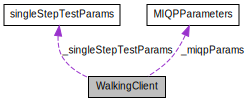
\includegraphics[width=350pt]{classWalkingClient__coll__graph}
\end{center}
\end{figure}
\subsection*{\-Public \-Member \-Functions}
\begin{DoxyCompactItemize}
\item 
\hyperlink{classWalkingClient_a6c9002a44a54814c4b482739824e39aa}{\-Walking\-Client} (std\-::shared\-\_\-ptr$<$ ocra\-::\-Model $>$ model\-Ptr, const int loop\-Period)
\item 
virtual \hyperlink{classWalkingClient_a1dbc0308f844aea6542750104fddf8e2}{$\sim$\-Walking\-Client} ()
\item 
bool \hyperlink{classWalkingClient_adb8f972f34cb39c69c02a7c3cb493b81}{configure} (yarp\-::os\-::\-Resource\-Finder \&rf)
\item 
void \hyperlink{classWalkingClient_aff3fabef11d9c8b747a422f879c26067}{print\-Help} ()
\item 
bool \hyperlink{classWalkingClient_a77e764f397231fe311a7a0f0d91a9b65}{query\-M\-I\-Q\-P\-Solution} (const int miqp\-Period, const int miqp\-Preview\-Period, const int client\-Period, \-Eigen\-::\-Vector\-Xd \&preview)
\item 
bool \hyperlink{classWalkingClient_a03ea2313c954a97aeb4d5b614f3e6caa}{read\-Foot\-Wrench} (\hyperlink{utils_8h_a4b6a8e135f90bd56e5a57a60efb42529}{\-F\-O\-O\-T} which\-Foot, \-Eigen\-::\-Vector\-Xd \&raw\-Wrench)
\item 
std\-::vector$<$ \-Eigen\-::\-Vector2d $>$ \hyperlink{classWalkingClient_a3185a8ede8bf8b1227f7dd540ba87e3c}{generate\-Z\-M\-P\-Trajectory\-T\-E\-S\-T} (const double t\-Trans, const double feet\-Separation, const double time\-Step, const int amplitude\-Fraction, const int \-N)
\item 
bool \hyperlink{classWalkingClient_a87e70046251149b4b7aff1dc57b3dcc4}{get\-Feet\-Separation} (\-Eigen\-::\-Vector3d \&sep)
\item 
bool \hyperlink{classWalkingClient_ae6d6c046a9a3e51771afe8b4c105b412}{publish3d\-Quantity} (yarp\-::os\-::\-Buffered\-Port$<$ yarp\-::os\-::\-Bottle $>$ \&port, \-Eigen\-::\-Vector3d \&value)
\item 
void \hyperlink{classWalkingClient_ae3c259f7615c85ce53a413f6e7ab4b76}{perform\-Z\-M\-P\-Test} (\hyperlink{utils_8h_afc01479a47f5a87462a54b6a9e11fffa}{\-Zmp\-Test\-Type} type)
\item 
void \hyperlink{classWalkingClient_a3b1217b7fa17f76f162be0e12e419d96}{perform\-Z\-M\-P\-Preview\-Test} (\hyperlink{utils_8h_afc01479a47f5a87462a54b6a9e11fffa}{\-Zmp\-Test\-Type} type)
\item 
void \hyperlink{classWalkingClient_a49fb64ddafa81f0a5f29a8c0fc5188bd}{perform\-Single\-Step\-Test} ()
\item 
void \hyperlink{classWalkingClient_adb2fbd66671321d046cf5e1ca74f5bc1}{stepping\-Test} ()
\item 
std\-::string \hyperlink{classWalkingClient_ae8f7dc629313df7d362e3edd6f45ae10}{compose\-Port\-Name} (std\-::string port\-Name)
\item 
void \hyperlink{classWalkingClient_acd9cf6d2c9a140f789437882d781d963}{find\-Z\-M\-P\-Preview\-Controller\-Params} (yarp\-::os\-::\-Resource\-Finder \&rf)
\item 
void \hyperlink{classWalkingClient_ab94cb8266e45f49e51396458df7f8708}{find\-General\-Tests\-Params} (yarp\-::os\-::\-Resource\-Finder \&rf)
\item 
void \hyperlink{classWalkingClient_a2a7372e6cad46efd380eb85e7547cf4e}{find\-C\-O\-M\-Lin\-Vel\-Const\-Ref\-Params} (yarp\-::os\-::\-Resource\-Finder \&rf)
\item 
void \hyperlink{classWalkingClient_ad8eb137c03025ce04cedd4eea58f7a6d}{find\-Z\-M\-P\-Const\-Ref\-Params} (yarp\-::os\-::\-Resource\-Finder \&rf)
\item 
void \hyperlink{classWalkingClient_a48e8e823e0a76a662722e05f6bd803e3}{find\-Single\-Step\-Test\-Params} (yarp\-::os\-::\-Resource\-Finder \&rf)
\item 
void \hyperlink{classWalkingClient_a6b8f21532c8207ec95b64f6548c3b6b1}{find\-Z\-M\-P\-Varying\-Reference\-Params} (yarp\-::os\-::\-Resource\-Finder \&rf)
\item 
void \hyperlink{classWalkingClient_accdb497fc22b293095290f3d63d5cf72}{find\-M\-I\-Q\-P\-Params} (yarp\-::os\-::\-Resource\-Finder \&rf)
\item 
void \hyperlink{classWalkingClient_af0f47f61db149b0beabb516f4f244dfc}{find\-Stepping\-Test\-Params} (yarp\-::os\-::\-Resource\-Finder \&rf)
\item 
void \hyperlink{classWalkingClient_ab4148804702e065310a903112bc10162}{transform\-Std\-Vector\-To\-Eigen\-Vector} (std\-::vector$<$ \-Eigen\-::\-Vector2d $>$ \&full\-Traj, int from, int \-Nc, \-Vector\-Xd \&output)
\item 
std\-::vector$<$ \-Eigen\-::\-Vector2d $>$ \hyperlink{classWalkingClient_a70b2375134ae55a041fbf30180ea3a8f}{generate\-Z\-M\-P\-Step\-Trajectory\-T\-E\-S\-T} (double feet\-Separation, double period, double duration, double rise\-Time, double constant\-Reference\-Y)
\item 
std\-::vector$<$ \-Eigen\-::\-Vector2d $>$ \hyperlink{classWalkingClient_ab5bd1eceec03d8b88ffe2b6b07d981c0}{generate\-Z\-M\-P\-Single\-Step\-Trajectory} (double period, double feet\-Separation)
\item 
void \hyperlink{classWalkingClient_a51ac091a481766030dcedf7327122c19}{generate\-Step\-Pattern} ()
\item 
std\-::vector$<$ \-Eigen\-::\-Vector2d $>$ \hyperlink{classWalkingClient_aebee5b71a15e0b990fb3dad36f335eb5}{generate\-Z\-M\-P\-Stepping\-Trajectory} ()
\item 
void \hyperlink{classWalkingClient_ab497c47c538b8ac2871ddd706c5e61a9}{start\-Steppin\-Mother\-Fucker} ()
\item 
void \hyperlink{classWalkingClient_aad39a3836319f9b7258d8eb129776b47}{prepare\-Andset\-Desired\-Co\-M\-Task\-State} (\-Eigen\-::\-Vector\-Xd com\-State, bool do\-Set)
\end{DoxyCompactItemize}
\subsection*{\-Public \-Attributes}
\begin{DoxyCompactItemize}
\item 
yarp\-::os\-::\-Buffered\-Port\*
$<$ yarp\-::sig\-::\-Vector $>$ \hyperlink{classWalkingClient_a88ee63ff6a341eccd458d24700383457}{port\-Wrench\-Left\-Foot}
\item 
yarp\-::os\-::\-Buffered\-Port\*
$<$ yarp\-::sig\-::\-Vector $>$ \hyperlink{classWalkingClient_a96321dc60e84c193f2dea6e85983ca67}{port\-Wrench\-Right\-Foot}
\end{DoxyCompactItemize}
\subsection*{\-Protected \-Member \-Functions}
\begin{DoxyCompactItemize}
\item 
virtual bool \hyperlink{classWalkingClient_aba6a03fe29a4e947bc6bc0c09a713b2a}{initialize} ()
\item 
virtual void \hyperlink{classWalkingClient_a3b36da9d7649865a13c9318dd73ebc7e}{release} ()
\item 
virtual void \hyperlink{classWalkingClient_afd997bb00534c57fe1b0d5f37f207386}{loop} ()
\end{DoxyCompactItemize}
\subsection*{\-Private \-Attributes}
\begin{DoxyCompactItemize}
\item 
std\-::vector$<$ \hyperlink{utils_8h_a4b6a8e135f90bd56e5a57a60efb42529}{\-F\-O\-O\-T} $>$ \hyperlink{classWalkingClient_acc23c96509280a29e7331cc1b0fe0576}{\-\_\-step\-Order}
\item 
\-Eigen\-::\-Matrix\-Xd \hyperlink{classWalkingClient_a7bce7b80a798dd4d46dfc93947ea4d31}{\-\_\-step\-Targets}
\item 
\-Eigen\-::\-Vector\-Xd \hyperlink{classWalkingClient_abddb902c1db56468913945eb8b81c55e}{\-\_\-step\-Target\-Durations}
\item 
bool \hyperlink{classWalkingClient_aeaed1c4beda89ebe62ba7e3e6c0902dd}{\-\_\-currently\-Stepping}
\item 
bool \hyperlink{classWalkingClient_a0006acb41bc17941086f841e7edeb5b3}{\-\_\-wait\-Before\-Next\-Step}
\item 
double \hyperlink{classWalkingClient_a2814e5c3372855c087226778925bafe1}{\-\_\-wait\-Time\-Start}
\item 
int \hyperlink{classWalkingClient_a7d122ec14817ae7ea6bc5b2aba404950}{\-\_\-current\-Step\-Index}
\item 
std\-::vector$<$ \-Eigen\-::\-Vector2d $>$ \hyperlink{classWalkingClient_a4f76ca724ed725f6f727828e30fcf628}{\-\_\-stepping\-Trajectory}
\item 
\hyperlink{structsteppingTestParams}{stepping\-Test\-Params} \hyperlink{classWalkingClient_ae806c00e966e6d121426288a017aaa7d}{\-\_\-stepping\-Test\-Params}
\item 
std\-::shared\-\_\-ptr$<$ \hyperlink{structZmpPreviewParams}{\-Zmp\-Preview\-Params} $>$ \hyperlink{classWalkingClient_a9a2cf2d6107ab91fc5bd1d82a3b85a84}{\-\_\-zmp\-Preview\-Params}
\item 
std\-::shared\-\_\-ptr\*
$<$ \hyperlink{classZmpPreviewController}{\-Zmp\-Preview\-Controller} $>$ \hyperlink{classWalkingClient_ae570aa07bed9e336eda93f331f3485fb}{\-\_\-zmp\-Preview\-Controller}
\item 
std\-::shared\-\_\-ptr\*
$<$ ocra\-\_\-recipes\-::\-Task\-Connection $>$ \hyperlink{classWalkingClient_aa798d6193535e80816f8107ee5fb2172}{\-\_\-com\-Task}
\item 
std\-::shared\-\_\-ptr$<$ \hyperlink{classMIQPController}{\-M\-I\-Q\-P\-Controller} $>$ \hyperlink{classWalkingClient_a5dd1abe90bf7182766548c93673af2df}{\-\_\-miqp\-Controller}
\item 
std\-::shared\-\_\-ptr$<$ \hyperlink{classStepController}{\-Step\-Controller} $>$ \hyperlink{classWalkingClient_aff3d76fc360548d6c0c0ea540a0b7509}{\-\_\-step\-Controller}
\item 
std\-::vector$<$ \-Eigen\-::\-Vector2d $>$ \hyperlink{classWalkingClient_a8b8a3d7fe6e12d49a0e72d05f9938564}{\-\_\-zmp\-Trajectory}
\item 
std\-::vector$<$ \-Eigen\-::\-Vector2d $>$ \hyperlink{classWalkingClient_a5d74b737b225cec818922a2b774eed9e}{\-\_\-single\-Step\-Trajectory}
\item 
ocra\-::\-Task\-State \hyperlink{classWalkingClient_a2625bf687aa3141f5a2404c8d9b3c392}{\-\_\-desired\-Com\-State}
\item 
\hyperlink{structMIQPParameters}{\-M\-I\-Q\-P\-Parameters} \hyperlink{classWalkingClient_a5035091f977f37b7d2df284015242d6c}{\-\_\-miqp\-Params}
\item 
\-Eigen\-::\-Vector\-Xd \hyperlink{classWalkingClient_a1c3fb4d182e33d6d9386e9bb05aa4ae8}{\-\_\-raw\-Left\-Foot\-Wrench}
\item 
\-Eigen\-::\-Vector\-Xd \hyperlink{classWalkingClient_a9df32e0c73632c5f869e5933e20def71}{\-\_\-raw\-Right\-Foot\-Wrench}
\item 
\-Eigen\-::\-Vector2d \hyperlink{classWalkingClient_aa784eac1247f0d858e2364e0c2bc25b2}{\-\_\-global\-Z\-M\-P}
\item 
\-Eigen\-::\-Vector2d \hyperlink{classWalkingClient_a549751e511e023d5fc73eccd1c185317}{\-\_\-previous\-C\-O\-M}
\item 
\-Eigen\-::\-Vector2d \hyperlink{classWalkingClient_aa0c7669193a8a42ed289c79523580033}{\-\_\-previous\-C\-O\-M\-Vel}
\item 
std\-::string \hyperlink{classWalkingClient_aff02b341d5e1f500dc9a849337319a8d}{\-\_\-client\-Name}
\item 
std\-::string \hyperlink{classWalkingClient_a67461634d7e8cb0234400b34fd2865e7}{\-\_\-robot}
\item 
bool \hyperlink{classWalkingClient_a4f9c8688537ddd8a487a212fbb279a9b}{\-\_\-is\-Test\-Run}
\item 
std\-::string \hyperlink{classWalkingClient_a35c00feb4e7dfa532e43241e855fec89}{\-\_\-test\-Type}
\item 
\hyperlink{utils_8h_afc01479a47f5a87462a54b6a9e11fffa}{\-Zmp\-Test\-Type} \hyperlink{classWalkingClient_a14576258d7fed1b36919145f1b56d74c}{\-\_\-zmp\-Test\-Type}
\item 
std\-::string \hyperlink{classWalkingClient_ade3bf018661152fc0404d3973ea30783}{\-\_\-home\-Data\-Dir}
\item 
double \hyperlink{classWalkingClient_a4e448bc147b41d97e0f17af6ebb0020f}{\-\_\-com\-Y\-Const\-Vel}
\item 
double \hyperlink{classWalkingClient_a9f19b1a1184cbdbf883cc374c6b6b88f}{\-\_\-stop\-Time\-Const\-Com\-Vel}
\item 
double \hyperlink{classWalkingClient_a6cba3194816a0be78a8b17d539806115}{\-\_\-zmp\-Y\-Const\-Ref}
\item 
double \hyperlink{classWalkingClient_a58b08317f6d8b825a21e1db8c7f0ff32}{\-\_\-stop\-Time\-Const\-Zmp}
\item 
double \hyperlink{classWalkingClient_aab1bac82d66908def9a36bede6bb24e2}{\-\_\-rise\-Time\-Const\-Zmp}
\item 
double \hyperlink{classWalkingClient_aa6b3bf5c2ed923a7a33a9ed461713d98}{\-\_\-trajectory\-Duration\-Const\-Zmp}
\item 
double \hyperlink{classWalkingClient_a7d15e2b9c9ada337280c46d6aadb54f8}{\-\_\-constant\-Reference\-Y}
\item 
\hyperlink{structsingleStepTestParams}{single\-Step\-Test\-Params} \hyperlink{classWalkingClient_a92adc07ae5221e5dde31483fe5d2deae}{\-\_\-single\-Step\-Test\-Params}
\item 
double \hyperlink{classWalkingClient_a144518766ec4eb9eeab230fcb291e20c}{\-\_\-t\-Trans}
\item 
int \hyperlink{classWalkingClient_aefb4ed994a32879a526f2bc8c962927f}{\-\_\-number\-Of\-Transitions}
\item 
int \hyperlink{classWalkingClient_ac548ce03ea9ceffb4b42981942f66dd0}{\-\_\-amplitude\-Fraction}
\item 
double \hyperlink{classWalkingClient_a2ed3837afa0c366f1cdef16b2a99b761}{\-\_\-stop\-Time\-Varying\-Zmp}
\item 
int \hyperlink{classWalkingClient_a8156c60725f7bda3de34ef0aae15bd16}{\-\_\-k}
\item 
yarp\-::os\-::\-Buffered\-Port\*
$<$ yarp\-::os\-::\-Bottle $>$ \hyperlink{classWalkingClient_af2e0817fa94ca802775addd22b09bf7a}{\-\_\-zmp\-Port}
\item 
yarp\-::os\-::\-Buffered\-Port\*
$<$ yarp\-::os\-::\-Bottle $>$ \hyperlink{classWalkingClient_a1b01264c9d9d403a68a149d86d1bc53f}{\-\_\-dcom\-Error\-Port}
\item 
yarp\-::os\-::\-Buffered\-Port\*
$<$ yarp\-::os\-::\-Bottle $>$ \hyperlink{classWalkingClient_a17369473b4fe2ff0eaecc7d41a8430c7}{\-\_\-d\-Com\-Des\-Port}
\item 
yarp\-::os\-::\-Buffered\-Port\*
$<$ yarp\-::os\-::\-Bottle $>$ \hyperlink{classWalkingClient_a1fbc9d7f1e967f24acda745028f865df}{\-\_\-d\-Com\-Cur\-Port}
\item 
yarp\-::os\-::\-Buffered\-Port\*
$<$ yarp\-::os\-::\-Bottle $>$ \hyperlink{classWalkingClient_acbac3e142471448b50dd605e4217b0d0}{\-\_\-zmp\-Des\-Port}
\item 
yarp\-::os\-::\-Buffered\-Port\*
$<$ yarp\-::os\-::\-Bottle $>$ \hyperlink{classWalkingClient_a546e6830e43d19ba7d8a8e808e28ef53}{\-\_\-zmp\-Cur\-Port}
\item 
yarp\-::os\-::\-Buffered\-Port\*
$<$ yarp\-::os\-::\-Bottle $>$ \hyperlink{classWalkingClient_a199a104e0d4d52deae07d88d8229b60d}{\-\_\-com\-Current}
\item 
yarp\-::os\-::\-Buffered\-Port\*
$<$ yarp\-::os\-::\-Bottle $>$ \hyperlink{classWalkingClient_a692d95b3e76a396d107b0c29a3d591f1}{\-\_\-ddcom\-Current}
\item 
yarp\-::os\-::\-Buffered\-Port\*
$<$ yarp\-::os\-::\-Bottle $>$ \hyperlink{classWalkingClient_a41b7320607812418af496b8b2c30204f}{\-\_\-ddcom\-From\-Z\-M\-P}
\item 
\-Vector\-Xd \hyperlink{classWalkingClient_abc3c504305c00a27e9fd38a8bf08ecda}{\-\_\-hkk\-Previous}
\item 
bool \hyperlink{classWalkingClient_ab645ecb2d55e28b57a64ca48ee638b1e}{\-\_\-first\-Loop}
\item 
\-Eigen\-::\-Vector\-Xd \hyperlink{classWalkingClient_af28b3cd3b1202f83e193b098572fbdd3}{zmp\-Ref\-In\-Preview\-Window}
\item 
\-Eigen\-::\-Vector\-Xd \hyperlink{classWalkingClient_ab3b1defedb6d79b5b6eaadd52bbad9f5}{com\-Vel\-Ref\-In\-Preview\-Window}
\item 
\-Eigen\-::\-Vector\-Xd \hyperlink{classWalkingClient_a0e5aee88e377029d79f57e778c583f18}{optimal\-U}
\item 
\-Eigen\-::\-Vector\-Xd \hyperlink{classWalkingClient_ab56a64a3f08320bb1b92671c6612f7b9}{\-\_\-\-X\-\_\-kn}
\end{DoxyCompactItemize}


\subsection{\-Constructor \& \-Destructor \-Documentation}
\hypertarget{classWalkingClient_a6c9002a44a54814c4b482739824e39aa}{\index{\-Walking\-Client@{\-Walking\-Client}!\-Walking\-Client@{\-Walking\-Client}}
\index{\-Walking\-Client@{\-Walking\-Client}!WalkingClient@{\-Walking\-Client}}
\subsubsection[{\-Walking\-Client}]{\setlength{\rightskip}{0pt plus 5cm}{\bf \-Walking\-Client\-::\-Walking\-Client} (
\begin{DoxyParamCaption}
\item[{std\-::shared\-\_\-ptr$<$ ocra\-::\-Model $>$}]{model\-Ptr, }
\item[{const int}]{loop\-Period}
\end{DoxyParamCaption}
)}}\label{classWalkingClient_a6c9002a44a54814c4b482739824e39aa}
\hypertarget{classWalkingClient_a1dbc0308f844aea6542750104fddf8e2}{\index{\-Walking\-Client@{\-Walking\-Client}!$\sim$\-Walking\-Client@{$\sim$\-Walking\-Client}}
\index{$\sim$\-Walking\-Client@{$\sim$\-Walking\-Client}!WalkingClient@{\-Walking\-Client}}
\subsubsection[{$\sim$\-Walking\-Client}]{\setlength{\rightskip}{0pt plus 5cm}{\bf \-Walking\-Client\-::$\sim$\-Walking\-Client} (
\begin{DoxyParamCaption}
{}
\end{DoxyParamCaption}
)\hspace{0.3cm}{\ttfamily  \mbox{[}virtual\mbox{]}}}}\label{classWalkingClient_a1dbc0308f844aea6542750104fddf8e2}


\subsection{\-Member \-Function \-Documentation}
\hypertarget{classWalkingClient_ae8f7dc629313df7d362e3edd6f45ae10}{\index{\-Walking\-Client@{\-Walking\-Client}!compose\-Port\-Name@{compose\-Port\-Name}}
\index{compose\-Port\-Name@{compose\-Port\-Name}!WalkingClient@{\-Walking\-Client}}
\subsubsection[{compose\-Port\-Name}]{\setlength{\rightskip}{0pt plus 5cm}std\-::string {\bf \-Walking\-Client\-::compose\-Port\-Name} (
\begin{DoxyParamCaption}
\item[{std\-::string}]{port\-Name}
\end{DoxyParamCaption}
)}}\label{classWalkingClient_ae8f7dc629313df7d362e3edd6f45ae10}
\-Composes a port name with the client name as the suffix. \-This client name is assumed to be passed through command line options or configuration file as per the policies of yarp's \-Resource \-Finder.


\begin{DoxyParams}{\-Parameters}
{\em port\-Name} & \-Name of the port without backslashes. e.\-g. \char`\"{}zmp\-Error\-:o\char`\"{} \\
\hline
\end{DoxyParams}
\begin{DoxyReturn}{\-Returns}
\-A client-\/name-\/prepended port name, e.\-g. \char`\"{}/walking\-Client/zmp\-Error\-:o\char`\"{} 
\end{DoxyReturn}
\hypertarget{classWalkingClient_adb8f972f34cb39c69c02a7c3cb493b81}{\index{\-Walking\-Client@{\-Walking\-Client}!configure@{configure}}
\index{configure@{configure}!WalkingClient@{\-Walking\-Client}}
\subsubsection[{configure}]{\setlength{\rightskip}{0pt plus 5cm}bool {\bf \-Walking\-Client\-::configure} (
\begin{DoxyParamCaption}
\item[{yarp\-::os\-::\-Resource\-Finder \&}]{rf}
\end{DoxyParamCaption}
)}}\label{classWalkingClient_adb8f972f34cb39c69c02a7c3cb493b81}
\-Takes all the parameters used by this client from configuration file and parses them through yarp's \-Resource \-Finder.

\-Details on group \mbox{[}\-Z\-M\-P\-\_\-\-C\-O\-N\-T\-R\-O\-L\-L\-E\-R\-\_\-\-P\-A\-R\-A\-M\-S\mbox{]} in walking-\/client.\-ini \-Options are\-: 0 -\/ \-Z\-M\-P\-\_\-\-C\-O\-N\-S\-T\-A\-N\-T\-\_\-\-R\-E\-F\-E\-R\-E\-N\-C\-E 1 -\/ \-Z\-M\-P\-\_\-\-V\-A\-R\-Y\-I\-N\-G\-\_\-\-R\-E\-F\-E\-R\-E\-N\-C\-E 2 -\/ \-C\-O\-M\-\_\-\-L\-I\-N\-\_\-\-V\-E\-L\-\_\-\-C\-O\-N\-S\-T\-A\-N\-T\-\_\-\-R\-E\-F\-E\-R\-E\-N\-C\-E \-Each of these tests are used to evaluate the correct gains to be used at each level of the control loops. \-These trajectorie will be used during the tests specified through the option 'test' which takes the values \char`\"{}zmp\-Preview\char`\"{} or \char`\"{}zmp\-Controller\char`\"{}. \-When using this client for the first time on a robot, the gains of the com\-Task in its corresponding task\-Set file must be tuned first as well and later those for the \hyperlink{classZmpController}{\-Zmp\-Controller} class. \-Therefore we recommend executing this client first as a way of testing the \char`\"{}low\char`\"{} level \-Com\-Task control in order to find good kp and kd. \-Do this by setting 'type' to 2. \-Data will be saved at the location you specify through the option 'home\-Data\-Dir'. \-After having a good \-C\-O\-M velocity tracking at the task level, you want to test the tracking of the zmp controller by setting 'type' to 0. \-A constant zmp reference is given and the controller gains kfx, kfy, kdx and kdy must be tuned accordingly. \-Finally, the tracking of varying zmp reference can be tested which takes the zmp from left to right, while the robot stands on both feet. \hypertarget{classWalkingClient_a2a7372e6cad46efd380eb85e7547cf4e}{\index{\-Walking\-Client@{\-Walking\-Client}!find\-C\-O\-M\-Lin\-Vel\-Const\-Ref\-Params@{find\-C\-O\-M\-Lin\-Vel\-Const\-Ref\-Params}}
\index{find\-C\-O\-M\-Lin\-Vel\-Const\-Ref\-Params@{find\-C\-O\-M\-Lin\-Vel\-Const\-Ref\-Params}!WalkingClient@{\-Walking\-Client}}
\subsubsection[{find\-C\-O\-M\-Lin\-Vel\-Const\-Ref\-Params}]{\setlength{\rightskip}{0pt plus 5cm}void {\bf \-Walking\-Client\-::find\-C\-O\-M\-Lin\-Vel\-Const\-Ref\-Params} (
\begin{DoxyParamCaption}
\item[{yarp\-::os\-::\-Resource\-Finder \&}]{rf}
\end{DoxyParamCaption}
)}}\label{classWalkingClient_a2a7372e6cad46efd380eb85e7547cf4e}
\hypertarget{classWalkingClient_ab94cb8266e45f49e51396458df7f8708}{\index{\-Walking\-Client@{\-Walking\-Client}!find\-General\-Tests\-Params@{find\-General\-Tests\-Params}}
\index{find\-General\-Tests\-Params@{find\-General\-Tests\-Params}!WalkingClient@{\-Walking\-Client}}
\subsubsection[{find\-General\-Tests\-Params}]{\setlength{\rightskip}{0pt plus 5cm}void {\bf \-Walking\-Client\-::find\-General\-Tests\-Params} (
\begin{DoxyParamCaption}
\item[{yarp\-::os\-::\-Resource\-Finder \&}]{rf}
\end{DoxyParamCaption}
)}}\label{classWalkingClient_ab94cb8266e45f49e51396458df7f8708}
\hypertarget{classWalkingClient_accdb497fc22b293095290f3d63d5cf72}{\index{\-Walking\-Client@{\-Walking\-Client}!find\-M\-I\-Q\-P\-Params@{find\-M\-I\-Q\-P\-Params}}
\index{find\-M\-I\-Q\-P\-Params@{find\-M\-I\-Q\-P\-Params}!WalkingClient@{\-Walking\-Client}}
\subsubsection[{find\-M\-I\-Q\-P\-Params}]{\setlength{\rightskip}{0pt plus 5cm}void {\bf \-Walking\-Client\-::find\-M\-I\-Q\-P\-Params} (
\begin{DoxyParamCaption}
\item[{yarp\-::os\-::\-Resource\-Finder \&}]{rf}
\end{DoxyParamCaption}
)}}\label{classWalkingClient_accdb497fc22b293095290f3d63d5cf72}
\hypertarget{classWalkingClient_a48e8e823e0a76a662722e05f6bd803e3}{\index{\-Walking\-Client@{\-Walking\-Client}!find\-Single\-Step\-Test\-Params@{find\-Single\-Step\-Test\-Params}}
\index{find\-Single\-Step\-Test\-Params@{find\-Single\-Step\-Test\-Params}!WalkingClient@{\-Walking\-Client}}
\subsubsection[{find\-Single\-Step\-Test\-Params}]{\setlength{\rightskip}{0pt plus 5cm}void {\bf \-Walking\-Client\-::find\-Single\-Step\-Test\-Params} (
\begin{DoxyParamCaption}
\item[{yarp\-::os\-::\-Resource\-Finder \&}]{rf}
\end{DoxyParamCaption}
)}}\label{classWalkingClient_a48e8e823e0a76a662722e05f6bd803e3}
\hypertarget{classWalkingClient_af0f47f61db149b0beabb516f4f244dfc}{\index{\-Walking\-Client@{\-Walking\-Client}!find\-Stepping\-Test\-Params@{find\-Stepping\-Test\-Params}}
\index{find\-Stepping\-Test\-Params@{find\-Stepping\-Test\-Params}!WalkingClient@{\-Walking\-Client}}
\subsubsection[{find\-Stepping\-Test\-Params}]{\setlength{\rightskip}{0pt plus 5cm}void {\bf \-Walking\-Client\-::find\-Stepping\-Test\-Params} (
\begin{DoxyParamCaption}
\item[{yarp\-::os\-::\-Resource\-Finder \&}]{rf}
\end{DoxyParamCaption}
)}}\label{classWalkingClient_af0f47f61db149b0beabb516f4f244dfc}
\hypertarget{classWalkingClient_ad8eb137c03025ce04cedd4eea58f7a6d}{\index{\-Walking\-Client@{\-Walking\-Client}!find\-Z\-M\-P\-Const\-Ref\-Params@{find\-Z\-M\-P\-Const\-Ref\-Params}}
\index{find\-Z\-M\-P\-Const\-Ref\-Params@{find\-Z\-M\-P\-Const\-Ref\-Params}!WalkingClient@{\-Walking\-Client}}
\subsubsection[{find\-Z\-M\-P\-Const\-Ref\-Params}]{\setlength{\rightskip}{0pt plus 5cm}void {\bf \-Walking\-Client\-::find\-Z\-M\-P\-Const\-Ref\-Params} (
\begin{DoxyParamCaption}
\item[{yarp\-::os\-::\-Resource\-Finder \&}]{rf}
\end{DoxyParamCaption}
)}}\label{classWalkingClient_ad8eb137c03025ce04cedd4eea58f7a6d}
\hypertarget{classWalkingClient_acd9cf6d2c9a140f789437882d781d963}{\index{\-Walking\-Client@{\-Walking\-Client}!find\-Z\-M\-P\-Preview\-Controller\-Params@{find\-Z\-M\-P\-Preview\-Controller\-Params}}
\index{find\-Z\-M\-P\-Preview\-Controller\-Params@{find\-Z\-M\-P\-Preview\-Controller\-Params}!WalkingClient@{\-Walking\-Client}}
\subsubsection[{find\-Z\-M\-P\-Preview\-Controller\-Params}]{\setlength{\rightskip}{0pt plus 5cm}void {\bf \-Walking\-Client\-::find\-Z\-M\-P\-Preview\-Controller\-Params} (
\begin{DoxyParamCaption}
\item[{yarp\-::os\-::\-Resource\-Finder \&}]{rf}
\end{DoxyParamCaption}
)}}\label{classWalkingClient_acd9cf6d2c9a140f789437882d781d963}
\hypertarget{classWalkingClient_a6b8f21532c8207ec95b64f6548c3b6b1}{\index{\-Walking\-Client@{\-Walking\-Client}!find\-Z\-M\-P\-Varying\-Reference\-Params@{find\-Z\-M\-P\-Varying\-Reference\-Params}}
\index{find\-Z\-M\-P\-Varying\-Reference\-Params@{find\-Z\-M\-P\-Varying\-Reference\-Params}!WalkingClient@{\-Walking\-Client}}
\subsubsection[{find\-Z\-M\-P\-Varying\-Reference\-Params}]{\setlength{\rightskip}{0pt plus 5cm}void {\bf \-Walking\-Client\-::find\-Z\-M\-P\-Varying\-Reference\-Params} (
\begin{DoxyParamCaption}
\item[{yarp\-::os\-::\-Resource\-Finder \&}]{rf}
\end{DoxyParamCaption}
)}}\label{classWalkingClient_a6b8f21532c8207ec95b64f6548c3b6b1}
\hypertarget{classWalkingClient_a51ac091a481766030dcedf7327122c19}{\index{\-Walking\-Client@{\-Walking\-Client}!generate\-Step\-Pattern@{generate\-Step\-Pattern}}
\index{generate\-Step\-Pattern@{generate\-Step\-Pattern}!WalkingClient@{\-Walking\-Client}}
\subsubsection[{generate\-Step\-Pattern}]{\setlength{\rightskip}{0pt plus 5cm}void {\bf \-Walking\-Client\-::generate\-Step\-Pattern} (
\begin{DoxyParamCaption}
{}
\end{DoxyParamCaption}
)}}\label{classWalkingClient_a51ac091a481766030dcedf7327122c19}
\-Generates a straight line step pattern with step targets, step order, and step durations. \-Used for testing. \hypertarget{classWalkingClient_ab5bd1eceec03d8b88ffe2b6b07d981c0}{\index{\-Walking\-Client@{\-Walking\-Client}!generate\-Z\-M\-P\-Single\-Step\-Trajectory@{generate\-Z\-M\-P\-Single\-Step\-Trajectory}}
\index{generate\-Z\-M\-P\-Single\-Step\-Trajectory@{generate\-Z\-M\-P\-Single\-Step\-Trajectory}!WalkingClient@{\-Walking\-Client}}
\subsubsection[{generate\-Z\-M\-P\-Single\-Step\-Trajectory}]{\setlength{\rightskip}{0pt plus 5cm}std\-::vector$<$ \-Eigen\-::\-Vector2d $>$ {\bf \-Walking\-Client\-::generate\-Z\-M\-P\-Single\-Step\-Trajectory} (
\begin{DoxyParamCaption}
\item[{double}]{period, }
\item[{double}]{feet\-Separation}
\end{DoxyParamCaption}
)}}\label{classWalkingClient_ab5bd1eceec03d8b88ffe2b6b07d981c0}
\hypertarget{classWalkingClient_aebee5b71a15e0b990fb3dad36f335eb5}{\index{\-Walking\-Client@{\-Walking\-Client}!generate\-Z\-M\-P\-Stepping\-Trajectory@{generate\-Z\-M\-P\-Stepping\-Trajectory}}
\index{generate\-Z\-M\-P\-Stepping\-Trajectory@{generate\-Z\-M\-P\-Stepping\-Trajectory}!WalkingClient@{\-Walking\-Client}}
\subsubsection[{generate\-Z\-M\-P\-Stepping\-Trajectory}]{\setlength{\rightskip}{0pt plus 5cm}std\-::vector$<$ \-Eigen\-::\-Vector2d $>$ {\bf \-Walking\-Client\-::generate\-Z\-M\-P\-Stepping\-Trajectory} (
\begin{DoxyParamCaption}
{}
\end{DoxyParamCaption}
)}}\label{classWalkingClient_aebee5b71a15e0b990fb3dad36f335eb5}
\-Generates a \-Z\-M\-P trajectory for the \-S\-T\-E\-P\-P\-I\-N\-G\-\_\-\-T\-E\-S\-T. \-Uses the step pattern generated by \hyperlink{classWalkingClient_a51ac091a481766030dcedf7327122c19}{generate\-Step\-Pattern}. \hypertarget{classWalkingClient_a70b2375134ae55a041fbf30180ea3a8f}{\index{\-Walking\-Client@{\-Walking\-Client}!generate\-Z\-M\-P\-Step\-Trajectory\-T\-E\-S\-T@{generate\-Z\-M\-P\-Step\-Trajectory\-T\-E\-S\-T}}
\index{generate\-Z\-M\-P\-Step\-Trajectory\-T\-E\-S\-T@{generate\-Z\-M\-P\-Step\-Trajectory\-T\-E\-S\-T}!WalkingClient@{\-Walking\-Client}}
\subsubsection[{generate\-Z\-M\-P\-Step\-Trajectory\-T\-E\-S\-T}]{\setlength{\rightskip}{0pt plus 5cm}std\-::vector$<$ \-Eigen\-::\-Vector2d $>$ {\bf \-Walking\-Client\-::generate\-Z\-M\-P\-Step\-Trajectory\-T\-E\-S\-T} (
\begin{DoxyParamCaption}
\item[{double}]{feet\-Separation, }
\item[{double}]{period, }
\item[{double}]{duration, }
\item[{double}]{rise\-Time, }
\item[{double}]{constant\-Reference\-Y}
\end{DoxyParamCaption}
)}}\label{classWalkingClient_a70b2375134ae55a041fbf30180ea3a8f}
\-Generates a step-\/like zmp trajectory for testing/assessment purposes. \-This assumes a world reference frame with positive x axis pointing forward and positive z axis pointing up.


\begin{DoxyParams}{\-Parameters}
{\em feet\-Separation} & \-Separation between the feet. \\
\hline
{\em period} & \hyperlink{classThread}{\-Thread} period in ms. \\
\hline
{\em duration} & \-Duration of the trajectory in seconds. \\
\hline
{\em rise\-Time} & \-Time in seconds at which the step should happen. \\
\hline
{\em constant\-Reference\-Y} & \-Value of the \\
\hline
\end{DoxyParams}
\begin{DoxyReturn}{\-Returns}
\-Vector of horizontal \-Z\-M\-P positions. 
\end{DoxyReturn}
\hypertarget{classWalkingClient_a3185a8ede8bf8b1227f7dd540ba87e3c}{\index{\-Walking\-Client@{\-Walking\-Client}!generate\-Z\-M\-P\-Trajectory\-T\-E\-S\-T@{generate\-Z\-M\-P\-Trajectory\-T\-E\-S\-T}}
\index{generate\-Z\-M\-P\-Trajectory\-T\-E\-S\-T@{generate\-Z\-M\-P\-Trajectory\-T\-E\-S\-T}!WalkingClient@{\-Walking\-Client}}
\subsubsection[{generate\-Z\-M\-P\-Trajectory\-T\-E\-S\-T}]{\setlength{\rightskip}{0pt plus 5cm}std\-::vector$<$ \-Eigen\-::\-Vector2d $>$ {\bf \-Walking\-Client\-::generate\-Z\-M\-P\-Trajectory\-T\-E\-S\-T} (
\begin{DoxyParamCaption}
\item[{const double}]{t\-Trans, }
\item[{const double}]{feet\-Separation, }
\item[{const double}]{time\-Step, }
\item[{const int}]{amplitude\-Fraction, }
\item[{const int}]{\-N}
\end{DoxyParamCaption}
)}}\label{classWalkingClient_a3185a8ede8bf8b1227f7dd540ba87e3c}
\-Generates a sinusoidal zmp trajectory on the $y$ expressed in the world reference frame. \-This is intended for testing purposes only.


\begin{DoxyParams}{\-Parameters}
{\em t\-Trans} & \-Time in which you want the \-Z\-M\-P to go from one foot to the other. \\
\hline
{\em feet\-Separation} & \-Separation between the feet in meters. \\
\hline
{\em time\-Step} & \-Desired time step. \\
\hline
{\em amplitude\-Fraction} & \-Fraction of the initial feet separation to determine max amplitude of movement. \\
\hline
{\em \-N} & \-Number of transitions (left to right or right to left).\\
\hline
\end{DoxyParams}
\begin{DoxyReturn}{\-Returns}
\-Trajectory of 2\-D \-Z\-M\-P points. 
\end{DoxyReturn}
\hypertarget{classWalkingClient_a87e70046251149b4b7aff1dc57b3dcc4}{\index{\-Walking\-Client@{\-Walking\-Client}!get\-Feet\-Separation@{get\-Feet\-Separation}}
\index{get\-Feet\-Separation@{get\-Feet\-Separation}!WalkingClient@{\-Walking\-Client}}
\subsubsection[{get\-Feet\-Separation}]{\setlength{\rightskip}{0pt plus 5cm}bool {\bf \-Walking\-Client\-::get\-Feet\-Separation} (
\begin{DoxyParamCaption}
\item[{\-Eigen\-::\-Vector3d \&}]{sep}
\end{DoxyParamCaption}
)}}\label{classWalkingClient_a87e70046251149b4b7aff1dc57b3dcc4}
\-Returns the current feet separation vector;


\begin{DoxyParams}{\-Parameters}
{\em sep} & \-Separation vector.\\
\hline
\end{DoxyParams}
\begin{DoxyReturn}{\-Returns}
\-True if all operations proceed well. \-False otherwise. 
\end{DoxyReturn}
\hypertarget{classWalkingClient_aba6a03fe29a4e947bc6bc0c09a713b2a}{\index{\-Walking\-Client@{\-Walking\-Client}!initialize@{initialize}}
\index{initialize@{initialize}!WalkingClient@{\-Walking\-Client}}
\subsubsection[{initialize}]{\setlength{\rightskip}{0pt plus 5cm}bool {\bf \-Walking\-Client\-::initialize} (
\begin{DoxyParamCaption}
{}
\end{DoxyParamCaption}
)\hspace{0.3cm}{\ttfamily  \mbox{[}protected, virtual\mbox{]}}}}\label{classWalkingClient_aba6a03fe29a4e947bc6bc0c09a713b2a}
\begin{DoxyRefDesc}{\-Todo}
\item[\hyperlink{todo__todo000011}{\-Todo}]\-Dummy initial \-C\-O\-M states reference! \end{DoxyRefDesc}
\hypertarget{classWalkingClient_afd997bb00534c57fe1b0d5f37f207386}{\index{\-Walking\-Client@{\-Walking\-Client}!loop@{loop}}
\index{loop@{loop}!WalkingClient@{\-Walking\-Client}}
\subsubsection[{loop}]{\setlength{\rightskip}{0pt plus 5cm}void {\bf \-Walking\-Client\-::loop} (
\begin{DoxyParamCaption}
{}
\end{DoxyParamCaption}
)\hspace{0.3cm}{\ttfamily  \mbox{[}protected, virtual\mbox{]}}}}\label{classWalkingClient_afd997bb00534c57fe1b0d5f37f207386}
\hypertarget{classWalkingClient_a49fb64ddafa81f0a5f29a8c0fc5188bd}{\index{\-Walking\-Client@{\-Walking\-Client}!perform\-Single\-Step\-Test@{perform\-Single\-Step\-Test}}
\index{perform\-Single\-Step\-Test@{perform\-Single\-Step\-Test}!WalkingClient@{\-Walking\-Client}}
\subsubsection[{perform\-Single\-Step\-Test}]{\setlength{\rightskip}{0pt plus 5cm}void {\bf \-Walking\-Client\-::perform\-Single\-Step\-Test} (
\begin{DoxyParamCaption}
{}
\end{DoxyParamCaption}
)}}\label{classWalkingClient_a49fb64ddafa81f0a5f29a8c0fc5188bd}
\hypertarget{classWalkingClient_a3b1217b7fa17f76f162be0e12e419d96}{\index{\-Walking\-Client@{\-Walking\-Client}!perform\-Z\-M\-P\-Preview\-Test@{perform\-Z\-M\-P\-Preview\-Test}}
\index{perform\-Z\-M\-P\-Preview\-Test@{perform\-Z\-M\-P\-Preview\-Test}!WalkingClient@{\-Walking\-Client}}
\subsubsection[{perform\-Z\-M\-P\-Preview\-Test}]{\setlength{\rightskip}{0pt plus 5cm}void {\bf \-Walking\-Client\-::perform\-Z\-M\-P\-Preview\-Test} (
\begin{DoxyParamCaption}
\item[{{\bf \-Zmp\-Test\-Type}}]{type}
\end{DoxyParamCaption}
)}}\label{classWalkingClient_a3b1217b7fa17f76f162be0e12e419d96}
\-Performs a zmp\-Preview\-Test for assessing and tuning of its parameters. \-This test has been succesfully performed with the i\-Cub platform on \-Gazebo using the following configuration set in walking-\/client.\-ini\-:

$|$ \-Parameter $|$ \-Value $|$ $|$ -\/-\/-\/-\/-\/-\/-\/-\/-\/-\/\-: $|$ \-:-\/-\/-\/-\/-\/$|$ $|$ \-Nc $|$ 200 $|$ $|$ nw $|$ 0.\-0 $|$ $|$ nb $|$ 1.\-0 $|$ $|$ nu $|$ 1e-\/6 $|$


\begin{DoxyParams}{\-Parameters}
{\em type} & \-Trajectory type. \\
\hline
\end{DoxyParams}
\begin{DoxySeeAlso}{\-See also}
\hyperlink{utils_8h_afc01479a47f5a87462a54b6a9e11fffa}{\-Zmp\-Test\-Type}. 
\end{DoxySeeAlso}
\hypertarget{classWalkingClient_ae3c259f7615c85ce53a413f6e7ab4b76}{\index{\-Walking\-Client@{\-Walking\-Client}!perform\-Z\-M\-P\-Test@{perform\-Z\-M\-P\-Test}}
\index{perform\-Z\-M\-P\-Test@{perform\-Z\-M\-P\-Test}!WalkingClient@{\-Walking\-Client}}
\subsubsection[{perform\-Z\-M\-P\-Test}]{\setlength{\rightskip}{0pt plus 5cm}void {\bf \-Walking\-Client\-::perform\-Z\-M\-P\-Test} (
\begin{DoxyParamCaption}
\item[{{\bf \-Zmp\-Test\-Type}}]{type}
\end{DoxyParamCaption}
)}}\label{classWalkingClient_ae3c259f7615c85ce53a413f6e7ab4b76}
\-Performs a zmp test for the specified type of trajectory.


\begin{DoxyParams}{\-Parameters}
{\em type} & \-See \-Zmp\-Test\-Type for possible options. \\
\hline
\end{DoxyParams}
\begin{DoxyNote}{\-Note}
\-To be deprecated as the zmp controller became unnecessary. 
\end{DoxyNote}
\hypertarget{classWalkingClient_aad39a3836319f9b7258d8eb129776b47}{\index{\-Walking\-Client@{\-Walking\-Client}!prepare\-Andset\-Desired\-Co\-M\-Task\-State@{prepare\-Andset\-Desired\-Co\-M\-Task\-State}}
\index{prepare\-Andset\-Desired\-Co\-M\-Task\-State@{prepare\-Andset\-Desired\-Co\-M\-Task\-State}!WalkingClient@{\-Walking\-Client}}
\subsubsection[{prepare\-Andset\-Desired\-Co\-M\-Task\-State}]{\setlength{\rightskip}{0pt plus 5cm}void {\bf \-Walking\-Client\-::prepare\-Andset\-Desired\-Co\-M\-Task\-State} (
\begin{DoxyParamCaption}
\item[{\-Eigen\-::\-Vector\-Xd}]{com\-State, }
\item[{bool}]{do\-Set}
\end{DoxyParamCaption}
)}}\label{classWalkingClient_aad39a3836319f9b7258d8eb129776b47}
\-Prepares an object of type ocra\-::\-Task\-State with the com state passed to this method and when do\-Set is true, applies the control to the robot.


\begin{DoxyParams}{\-Parameters}
{\em com\-State} & 6-\/dim \-Co\-M state vector (horizontal dynamics). \\
\hline
{\em do\-Set} & \-True if the desired state is to be set. \-False otherwise. \\
\hline
\end{DoxyParams}
\begin{DoxyRefDesc}{\-Todo}
\item[\hyperlink{todo__todo000010}{\-Todo}]\-Change input to this method to just com acceleration. \end{DoxyRefDesc}
\hypertarget{classWalkingClient_aff3fabef11d9c8b747a422f879c26067}{\index{\-Walking\-Client@{\-Walking\-Client}!print\-Help@{print\-Help}}
\index{print\-Help@{print\-Help}!WalkingClient@{\-Walking\-Client}}
\subsubsection[{print\-Help}]{\setlength{\rightskip}{0pt plus 5cm}void {\bf \-Walking\-Client\-::print\-Help} (
\begin{DoxyParamCaption}
{}
\end{DoxyParamCaption}
)}}\label{classWalkingClient_aff3fabef11d9c8b747a422f879c26067}
\-Prints a list of options accepted by the client. \hypertarget{classWalkingClient_ae6d6c046a9a3e51771afe8b4c105b412}{\index{\-Walking\-Client@{\-Walking\-Client}!publish3d\-Quantity@{publish3d\-Quantity}}
\index{publish3d\-Quantity@{publish3d\-Quantity}!WalkingClient@{\-Walking\-Client}}
\subsubsection[{publish3d\-Quantity}]{\setlength{\rightskip}{0pt plus 5cm}bool {\bf \-Walking\-Client\-::publish3d\-Quantity} (
\begin{DoxyParamCaption}
\item[{yarp\-::os\-::\-Buffered\-Port$<$ yarp\-::os\-::\-Bottle $>$ \&}]{port, }
\item[{\-Eigen\-::\-Vector3d \&}]{value}
\end{DoxyParamCaption}
)}}\label{classWalkingClient_ae6d6c046a9a3e51771afe8b4c105b412}
\-Write the \-Z\-M\-P error (externally computed, thus, any zmp related measurement) to a port.


\begin{DoxyParams}{\-Parameters}
{\em zmp\-Error} & $\mathbf{p} - \mathbf{p_d}$\\
\hline
\end{DoxyParams}
\begin{DoxyReturn}{\-Returns}
\-True if writing is successful, false otherwise. 
\end{DoxyReturn}
\hypertarget{classWalkingClient_a77e764f397231fe311a7a0f0d91a9b65}{\index{\-Walking\-Client@{\-Walking\-Client}!query\-M\-I\-Q\-P\-Solution@{query\-M\-I\-Q\-P\-Solution}}
\index{query\-M\-I\-Q\-P\-Solution@{query\-M\-I\-Q\-P\-Solution}!WalkingClient@{\-Walking\-Client}}
\subsubsection[{query\-M\-I\-Q\-P\-Solution}]{\setlength{\rightskip}{0pt plus 5cm}bool {\bf \-Walking\-Client\-::query\-M\-I\-Q\-P\-Solution} (
\begin{DoxyParamCaption}
\item[{const int}]{miqp\-Period, }
\item[{const int}]{miqp\-Preview\-Period, }
\item[{const int}]{client\-Period, }
\item[{\-Eigen\-::\-Vector\-Xd \&}]{preview}
\end{DoxyParamCaption}
)}}\label{classWalkingClient_a77e764f397231fe311a7a0f0d91a9b65}
\-If miqp\-Period/client\-Period samples have passed, this method asks for the \hyperlink{namespaceMIQP}{\-M\-I\-Q\-P} solution.


\begin{DoxyParams}[1]{\-Parameters}
 & {\em miqp\-Period} & \-Period of the \hyperlink{namespaceMIQP}{\-M\-I\-Q\-P} thread. \\
\hline
 & {\em miqp\-Preview\-Period} & \-Period used to discretize the \hyperlink{namespaceMIQP}{\-M\-I\-Q\-P} \\
\hline
 & {\em client\-Period} & \-Period of the current client thread. \\
\hline
\mbox{\tt out}  & {\em \-Preview} & solution from the \hyperlink{namespaceMIQP}{\-M\-I\-Q\-P}. \\
\hline
\end{DoxyParams}
\begin{DoxyReturn}{\-Returns}
\-True if the right amount of time has passed, false otherwise. 
\end{DoxyReturn}
\hypertarget{classWalkingClient_a03ea2313c954a97aeb4d5b614f3e6caa}{\index{\-Walking\-Client@{\-Walking\-Client}!read\-Foot\-Wrench@{read\-Foot\-Wrench}}
\index{read\-Foot\-Wrench@{read\-Foot\-Wrench}!WalkingClient@{\-Walking\-Client}}
\subsubsection[{read\-Foot\-Wrench}]{\setlength{\rightskip}{0pt plus 5cm}bool {\bf \-Walking\-Client\-::read\-Foot\-Wrench} (
\begin{DoxyParamCaption}
\item[{{\bf \-F\-O\-O\-T}}]{which\-Foot, }
\item[{\-Eigen\-::\-Vector\-Xd \&}]{raw\-Wrench}
\end{DoxyParamCaption}
)}}\label{classWalkingClient_a03ea2313c954a97aeb4d5b614f3e6caa}
\-Reads the raw wrench published for the corresponding analog force/torque sensors in i\-Cub's feet.


\begin{DoxyParams}{\-Parameters}
{\em which\-Foot} & \-For which foot is the measurement read. \\
\hline
{\em raw\-Wrench} & \-Result of the reading. \\
\hline
\end{DoxyParams}
\begin{DoxyReturn}{\-Returns}
\-True if reading is successful, false otherwise. 
\end{DoxyReturn}
\hypertarget{classWalkingClient_a3b36da9d7649865a13c9318dd73ebc7e}{\index{\-Walking\-Client@{\-Walking\-Client}!release@{release}}
\index{release@{release}!WalkingClient@{\-Walking\-Client}}
\subsubsection[{release}]{\setlength{\rightskip}{0pt plus 5cm}void {\bf \-Walking\-Client\-::release} (
\begin{DoxyParamCaption}
{}
\end{DoxyParamCaption}
)\hspace{0.3cm}{\ttfamily  \mbox{[}protected, virtual\mbox{]}}}}\label{classWalkingClient_a3b36da9d7649865a13c9318dd73ebc7e}
\hypertarget{classWalkingClient_ab497c47c538b8ac2871ddd706c5e61a9}{\index{\-Walking\-Client@{\-Walking\-Client}!start\-Steppin\-Mother\-Fucker@{start\-Steppin\-Mother\-Fucker}}
\index{start\-Steppin\-Mother\-Fucker@{start\-Steppin\-Mother\-Fucker}!WalkingClient@{\-Walking\-Client}}
\subsubsection[{start\-Steppin\-Mother\-Fucker}]{\setlength{\rightskip}{0pt plus 5cm}void {\bf \-Walking\-Client\-::start\-Steppin\-Mother\-Fucker} (
\begin{DoxyParamCaption}
{}
\end{DoxyParamCaption}
)}}\label{classWalkingClient_ab497c47c538b8ac2871ddd706c5e61a9}
\-Manages the step switching for the \-S\-T\-E\-P\-P\-I\-N\-G\-\_\-\-T\-E\-S\-T. \hypertarget{classWalkingClient_adb2fbd66671321d046cf5e1ca74f5bc1}{\index{\-Walking\-Client@{\-Walking\-Client}!stepping\-Test@{stepping\-Test}}
\index{stepping\-Test@{stepping\-Test}!WalkingClient@{\-Walking\-Client}}
\subsubsection[{stepping\-Test}]{\setlength{\rightskip}{0pt plus 5cm}void {\bf \-Walking\-Client\-::stepping\-Test} (
\begin{DoxyParamCaption}
{}
\end{DoxyParamCaption}
)}}\label{classWalkingClient_adb2fbd66671321d046cf5e1ca74f5bc1}
\-A test where the robot steps forward in a straight line. \-Only uses \-Z\-M\-P controller. \hypertarget{classWalkingClient_ab4148804702e065310a903112bc10162}{\index{\-Walking\-Client@{\-Walking\-Client}!transform\-Std\-Vector\-To\-Eigen\-Vector@{transform\-Std\-Vector\-To\-Eigen\-Vector}}
\index{transform\-Std\-Vector\-To\-Eigen\-Vector@{transform\-Std\-Vector\-To\-Eigen\-Vector}!WalkingClient@{\-Walking\-Client}}
\subsubsection[{transform\-Std\-Vector\-To\-Eigen\-Vector}]{\setlength{\rightskip}{0pt plus 5cm}void {\bf \-Walking\-Client\-::transform\-Std\-Vector\-To\-Eigen\-Vector} (
\begin{DoxyParamCaption}
\item[{std\-::vector$<$ \-Eigen\-::\-Vector2d $>$ \&}]{full\-Traj, }
\item[{int}]{from, }
\item[{int}]{\-Nc, }
\item[{\-Vector\-Xd \&}]{output}
\end{DoxyParamCaption}
)}}\label{classWalkingClient_ab4148804702e065310a903112bc10162}
\-Takes an std\-::\-Vector of \-Z\-M\-P trajectories at time $k$ and outputs the \-Z\-M\-P samples from time $k$ until $k + N_c$s, i.\-e. the \-Z\-M\-P preview window.


\begin{DoxyParams}{\-Parameters}
{\em full\-Traj} & \-Vector of horizontal \-Z\-M\-P positions. \\
\hline
{\em from} & \-Index in the vector corresponding to the current time instant. \\
\hline
{\em \-Nc} & \-Length of the preview window. \\
\hline
{\em output} & \-Z\-M\-P samples in the preview window. \\
\hline
\end{DoxyParams}


\subsection{\-Member \-Data \-Documentation}
\hypertarget{classWalkingClient_ac548ce03ea9ceffb4b42981942f66dd0}{\index{\-Walking\-Client@{\-Walking\-Client}!\-\_\-amplitude\-Fraction@{\-\_\-amplitude\-Fraction}}
\index{\-\_\-amplitude\-Fraction@{\-\_\-amplitude\-Fraction}!WalkingClient@{\-Walking\-Client}}
\subsubsection[{\-\_\-amplitude\-Fraction}]{\setlength{\rightskip}{0pt plus 5cm}int {\bf \-Walking\-Client\-::\-\_\-amplitude\-Fraction}\hspace{0.3cm}{\ttfamily  \mbox{[}private\mbox{]}}}}\label{classWalkingClient_ac548ce03ea9ceffb4b42981942f66dd0}
\hypertarget{classWalkingClient_aff02b341d5e1f500dc9a849337319a8d}{\index{\-Walking\-Client@{\-Walking\-Client}!\-\_\-client\-Name@{\-\_\-client\-Name}}
\index{\-\_\-client\-Name@{\-\_\-client\-Name}!WalkingClient@{\-Walking\-Client}}
\subsubsection[{\-\_\-client\-Name}]{\setlength{\rightskip}{0pt plus 5cm}std\-::string {\bf \-Walking\-Client\-::\-\_\-client\-Name}\hspace{0.3cm}{\ttfamily  \mbox{[}private\mbox{]}}}}\label{classWalkingClient_aff02b341d5e1f500dc9a849337319a8d}
\hypertarget{classWalkingClient_a199a104e0d4d52deae07d88d8229b60d}{\index{\-Walking\-Client@{\-Walking\-Client}!\-\_\-com\-Current@{\-\_\-com\-Current}}
\index{\-\_\-com\-Current@{\-\_\-com\-Current}!WalkingClient@{\-Walking\-Client}}
\subsubsection[{\-\_\-com\-Current}]{\setlength{\rightskip}{0pt plus 5cm}yarp\-::os\-::\-Buffered\-Port$<$yarp\-::os\-::\-Bottle$>$ {\bf \-Walking\-Client\-::\-\_\-com\-Current}\hspace{0.3cm}{\ttfamily  \mbox{[}private\mbox{]}}}}\label{classWalkingClient_a199a104e0d4d52deae07d88d8229b60d}
\hypertarget{classWalkingClient_aa798d6193535e80816f8107ee5fb2172}{\index{\-Walking\-Client@{\-Walking\-Client}!\-\_\-com\-Task@{\-\_\-com\-Task}}
\index{\-\_\-com\-Task@{\-\_\-com\-Task}!WalkingClient@{\-Walking\-Client}}
\subsubsection[{\-\_\-com\-Task}]{\setlength{\rightskip}{0pt plus 5cm}std\-::shared\-\_\-ptr$<$ocra\-\_\-recipes\-::\-Task\-Connection$>$ {\bf \-Walking\-Client\-::\-\_\-com\-Task}\hspace{0.3cm}{\ttfamily  \mbox{[}private\mbox{]}}}}\label{classWalkingClient_aa798d6193535e80816f8107ee5fb2172}
\hypertarget{classWalkingClient_a4e448bc147b41d97e0f17af6ebb0020f}{\index{\-Walking\-Client@{\-Walking\-Client}!\-\_\-com\-Y\-Const\-Vel@{\-\_\-com\-Y\-Const\-Vel}}
\index{\-\_\-com\-Y\-Const\-Vel@{\-\_\-com\-Y\-Const\-Vel}!WalkingClient@{\-Walking\-Client}}
\subsubsection[{\-\_\-com\-Y\-Const\-Vel}]{\setlength{\rightskip}{0pt plus 5cm}double {\bf \-Walking\-Client\-::\-\_\-com\-Y\-Const\-Vel}\hspace{0.3cm}{\ttfamily  \mbox{[}private\mbox{]}}}}\label{classWalkingClient_a4e448bc147b41d97e0f17af6ebb0020f}
\hypertarget{classWalkingClient_a7d15e2b9c9ada337280c46d6aadb54f8}{\index{\-Walking\-Client@{\-Walking\-Client}!\-\_\-constant\-Reference\-Y@{\-\_\-constant\-Reference\-Y}}
\index{\-\_\-constant\-Reference\-Y@{\-\_\-constant\-Reference\-Y}!WalkingClient@{\-Walking\-Client}}
\subsubsection[{\-\_\-constant\-Reference\-Y}]{\setlength{\rightskip}{0pt plus 5cm}double {\bf \-Walking\-Client\-::\-\_\-constant\-Reference\-Y}\hspace{0.3cm}{\ttfamily  \mbox{[}private\mbox{]}}}}\label{classWalkingClient_a7d15e2b9c9ada337280c46d6aadb54f8}
\hypertarget{classWalkingClient_aeaed1c4beda89ebe62ba7e3e6c0902dd}{\index{\-Walking\-Client@{\-Walking\-Client}!\-\_\-currently\-Stepping@{\-\_\-currently\-Stepping}}
\index{\-\_\-currently\-Stepping@{\-\_\-currently\-Stepping}!WalkingClient@{\-Walking\-Client}}
\subsubsection[{\-\_\-currently\-Stepping}]{\setlength{\rightskip}{0pt plus 5cm}bool {\bf \-Walking\-Client\-::\-\_\-currently\-Stepping}\hspace{0.3cm}{\ttfamily  \mbox{[}private\mbox{]}}}}\label{classWalkingClient_aeaed1c4beda89ebe62ba7e3e6c0902dd}
\hypertarget{classWalkingClient_a7d122ec14817ae7ea6bc5b2aba404950}{\index{\-Walking\-Client@{\-Walking\-Client}!\-\_\-current\-Step\-Index@{\-\_\-current\-Step\-Index}}
\index{\-\_\-current\-Step\-Index@{\-\_\-current\-Step\-Index}!WalkingClient@{\-Walking\-Client}}
\subsubsection[{\-\_\-current\-Step\-Index}]{\setlength{\rightskip}{0pt plus 5cm}int {\bf \-Walking\-Client\-::\-\_\-current\-Step\-Index}\hspace{0.3cm}{\ttfamily  \mbox{[}private\mbox{]}}}}\label{classWalkingClient_a7d122ec14817ae7ea6bc5b2aba404950}
\hypertarget{classWalkingClient_a1fbc9d7f1e967f24acda745028f865df}{\index{\-Walking\-Client@{\-Walking\-Client}!\-\_\-d\-Com\-Cur\-Port@{\-\_\-d\-Com\-Cur\-Port}}
\index{\-\_\-d\-Com\-Cur\-Port@{\-\_\-d\-Com\-Cur\-Port}!WalkingClient@{\-Walking\-Client}}
\subsubsection[{\-\_\-d\-Com\-Cur\-Port}]{\setlength{\rightskip}{0pt plus 5cm}yarp\-::os\-::\-Buffered\-Port$<$yarp\-::os\-::\-Bottle$>$ {\bf \-Walking\-Client\-::\-\_\-d\-Com\-Cur\-Port}\hspace{0.3cm}{\ttfamily  \mbox{[}private\mbox{]}}}}\label{classWalkingClient_a1fbc9d7f1e967f24acda745028f865df}
\hypertarget{classWalkingClient_a17369473b4fe2ff0eaecc7d41a8430c7}{\index{\-Walking\-Client@{\-Walking\-Client}!\-\_\-d\-Com\-Des\-Port@{\-\_\-d\-Com\-Des\-Port}}
\index{\-\_\-d\-Com\-Des\-Port@{\-\_\-d\-Com\-Des\-Port}!WalkingClient@{\-Walking\-Client}}
\subsubsection[{\-\_\-d\-Com\-Des\-Port}]{\setlength{\rightskip}{0pt plus 5cm}yarp\-::os\-::\-Buffered\-Port$<$yarp\-::os\-::\-Bottle$>$ {\bf \-Walking\-Client\-::\-\_\-d\-Com\-Des\-Port}\hspace{0.3cm}{\ttfamily  \mbox{[}private\mbox{]}}}}\label{classWalkingClient_a17369473b4fe2ff0eaecc7d41a8430c7}
\hypertarget{classWalkingClient_a1b01264c9d9d403a68a149d86d1bc53f}{\index{\-Walking\-Client@{\-Walking\-Client}!\-\_\-dcom\-Error\-Port@{\-\_\-dcom\-Error\-Port}}
\index{\-\_\-dcom\-Error\-Port@{\-\_\-dcom\-Error\-Port}!WalkingClient@{\-Walking\-Client}}
\subsubsection[{\-\_\-dcom\-Error\-Port}]{\setlength{\rightskip}{0pt plus 5cm}yarp\-::os\-::\-Buffered\-Port$<$yarp\-::os\-::\-Bottle$>$ {\bf \-Walking\-Client\-::\-\_\-dcom\-Error\-Port}\hspace{0.3cm}{\ttfamily  \mbox{[}private\mbox{]}}}}\label{classWalkingClient_a1b01264c9d9d403a68a149d86d1bc53f}
\hypertarget{classWalkingClient_a692d95b3e76a396d107b0c29a3d591f1}{\index{\-Walking\-Client@{\-Walking\-Client}!\-\_\-ddcom\-Current@{\-\_\-ddcom\-Current}}
\index{\-\_\-ddcom\-Current@{\-\_\-ddcom\-Current}!WalkingClient@{\-Walking\-Client}}
\subsubsection[{\-\_\-ddcom\-Current}]{\setlength{\rightskip}{0pt plus 5cm}yarp\-::os\-::\-Buffered\-Port$<$yarp\-::os\-::\-Bottle$>$ {\bf \-Walking\-Client\-::\-\_\-ddcom\-Current}\hspace{0.3cm}{\ttfamily  \mbox{[}private\mbox{]}}}}\label{classWalkingClient_a692d95b3e76a396d107b0c29a3d591f1}
\hypertarget{classWalkingClient_a41b7320607812418af496b8b2c30204f}{\index{\-Walking\-Client@{\-Walking\-Client}!\-\_\-ddcom\-From\-Z\-M\-P@{\-\_\-ddcom\-From\-Z\-M\-P}}
\index{\-\_\-ddcom\-From\-Z\-M\-P@{\-\_\-ddcom\-From\-Z\-M\-P}!WalkingClient@{\-Walking\-Client}}
\subsubsection[{\-\_\-ddcom\-From\-Z\-M\-P}]{\setlength{\rightskip}{0pt plus 5cm}yarp\-::os\-::\-Buffered\-Port$<$yarp\-::os\-::\-Bottle$>$ {\bf \-Walking\-Client\-::\-\_\-ddcom\-From\-Z\-M\-P}\hspace{0.3cm}{\ttfamily  \mbox{[}private\mbox{]}}}}\label{classWalkingClient_a41b7320607812418af496b8b2c30204f}
\hypertarget{classWalkingClient_a2625bf687aa3141f5a2404c8d9b3c392}{\index{\-Walking\-Client@{\-Walking\-Client}!\-\_\-desired\-Com\-State@{\-\_\-desired\-Com\-State}}
\index{\-\_\-desired\-Com\-State@{\-\_\-desired\-Com\-State}!WalkingClient@{\-Walking\-Client}}
\subsubsection[{\-\_\-desired\-Com\-State}]{\setlength{\rightskip}{0pt plus 5cm}ocra\-::\-Task\-State {\bf \-Walking\-Client\-::\-\_\-desired\-Com\-State}\hspace{0.3cm}{\ttfamily  \mbox{[}private\mbox{]}}}}\label{classWalkingClient_a2625bf687aa3141f5a2404c8d9b3c392}
\hypertarget{classWalkingClient_ab645ecb2d55e28b57a64ca48ee638b1e}{\index{\-Walking\-Client@{\-Walking\-Client}!\-\_\-first\-Loop@{\-\_\-first\-Loop}}
\index{\-\_\-first\-Loop@{\-\_\-first\-Loop}!WalkingClient@{\-Walking\-Client}}
\subsubsection[{\-\_\-first\-Loop}]{\setlength{\rightskip}{0pt plus 5cm}bool {\bf \-Walking\-Client\-::\-\_\-first\-Loop}\hspace{0.3cm}{\ttfamily  \mbox{[}private\mbox{]}}}}\label{classWalkingClient_ab645ecb2d55e28b57a64ca48ee638b1e}
\hypertarget{classWalkingClient_aa784eac1247f0d858e2364e0c2bc25b2}{\index{\-Walking\-Client@{\-Walking\-Client}!\-\_\-global\-Z\-M\-P@{\-\_\-global\-Z\-M\-P}}
\index{\-\_\-global\-Z\-M\-P@{\-\_\-global\-Z\-M\-P}!WalkingClient@{\-Walking\-Client}}
\subsubsection[{\-\_\-global\-Z\-M\-P}]{\setlength{\rightskip}{0pt plus 5cm}\-Eigen\-::\-Vector2d {\bf \-Walking\-Client\-::\-\_\-global\-Z\-M\-P}\hspace{0.3cm}{\ttfamily  \mbox{[}private\mbox{]}}}}\label{classWalkingClient_aa784eac1247f0d858e2364e0c2bc25b2}
\hypertarget{classWalkingClient_abc3c504305c00a27e9fd38a8bf08ecda}{\index{\-Walking\-Client@{\-Walking\-Client}!\-\_\-hkk\-Previous@{\-\_\-hkk\-Previous}}
\index{\-\_\-hkk\-Previous@{\-\_\-hkk\-Previous}!WalkingClient@{\-Walking\-Client}}
\subsubsection[{\-\_\-hkk\-Previous}]{\setlength{\rightskip}{0pt plus 5cm}\-Vector\-Xd {\bf \-Walking\-Client\-::\-\_\-hkk\-Previous}\hspace{0.3cm}{\ttfamily  \mbox{[}private\mbox{]}}}}\label{classWalkingClient_abc3c504305c00a27e9fd38a8bf08ecda}
\hypertarget{classWalkingClient_ade3bf018661152fc0404d3973ea30783}{\index{\-Walking\-Client@{\-Walking\-Client}!\-\_\-home\-Data\-Dir@{\-\_\-home\-Data\-Dir}}
\index{\-\_\-home\-Data\-Dir@{\-\_\-home\-Data\-Dir}!WalkingClient@{\-Walking\-Client}}
\subsubsection[{\-\_\-home\-Data\-Dir}]{\setlength{\rightskip}{0pt plus 5cm}std\-::string {\bf \-Walking\-Client\-::\-\_\-home\-Data\-Dir}\hspace{0.3cm}{\ttfamily  \mbox{[}private\mbox{]}}}}\label{classWalkingClient_ade3bf018661152fc0404d3973ea30783}
\hypertarget{classWalkingClient_a4f9c8688537ddd8a487a212fbb279a9b}{\index{\-Walking\-Client@{\-Walking\-Client}!\-\_\-is\-Test\-Run@{\-\_\-is\-Test\-Run}}
\index{\-\_\-is\-Test\-Run@{\-\_\-is\-Test\-Run}!WalkingClient@{\-Walking\-Client}}
\subsubsection[{\-\_\-is\-Test\-Run}]{\setlength{\rightskip}{0pt plus 5cm}bool {\bf \-Walking\-Client\-::\-\_\-is\-Test\-Run}\hspace{0.3cm}{\ttfamily  \mbox{[}private\mbox{]}}}}\label{classWalkingClient_a4f9c8688537ddd8a487a212fbb279a9b}
\hypertarget{classWalkingClient_a8156c60725f7bda3de34ef0aae15bd16}{\index{\-Walking\-Client@{\-Walking\-Client}!\-\_\-k@{\-\_\-k}}
\index{\-\_\-k@{\-\_\-k}!WalkingClient@{\-Walking\-Client}}
\subsubsection[{\-\_\-k}]{\setlength{\rightskip}{0pt plus 5cm}int {\bf \-Walking\-Client\-::\-\_\-k}\hspace{0.3cm}{\ttfamily  \mbox{[}private\mbox{]}}}}\label{classWalkingClient_a8156c60725f7bda3de34ef0aae15bd16}
\hypertarget{classWalkingClient_a5dd1abe90bf7182766548c93673af2df}{\index{\-Walking\-Client@{\-Walking\-Client}!\-\_\-miqp\-Controller@{\-\_\-miqp\-Controller}}
\index{\-\_\-miqp\-Controller@{\-\_\-miqp\-Controller}!WalkingClient@{\-Walking\-Client}}
\subsubsection[{\-\_\-miqp\-Controller}]{\setlength{\rightskip}{0pt plus 5cm}std\-::shared\-\_\-ptr$<${\bf \-M\-I\-Q\-P\-Controller}$>$ {\bf \-Walking\-Client\-::\-\_\-miqp\-Controller}\hspace{0.3cm}{\ttfamily  \mbox{[}private\mbox{]}}}}\label{classWalkingClient_a5dd1abe90bf7182766548c93673af2df}
\hypertarget{classWalkingClient_a5035091f977f37b7d2df284015242d6c}{\index{\-Walking\-Client@{\-Walking\-Client}!\-\_\-miqp\-Params@{\-\_\-miqp\-Params}}
\index{\-\_\-miqp\-Params@{\-\_\-miqp\-Params}!WalkingClient@{\-Walking\-Client}}
\subsubsection[{\-\_\-miqp\-Params}]{\setlength{\rightskip}{0pt plus 5cm}{\bf \-M\-I\-Q\-P\-Parameters} {\bf \-Walking\-Client\-::\-\_\-miqp\-Params}\hspace{0.3cm}{\ttfamily  \mbox{[}private\mbox{]}}}}\label{classWalkingClient_a5035091f977f37b7d2df284015242d6c}
\hypertarget{classWalkingClient_aefb4ed994a32879a526f2bc8c962927f}{\index{\-Walking\-Client@{\-Walking\-Client}!\-\_\-number\-Of\-Transitions@{\-\_\-number\-Of\-Transitions}}
\index{\-\_\-number\-Of\-Transitions@{\-\_\-number\-Of\-Transitions}!WalkingClient@{\-Walking\-Client}}
\subsubsection[{\-\_\-number\-Of\-Transitions}]{\setlength{\rightskip}{0pt plus 5cm}int {\bf \-Walking\-Client\-::\-\_\-number\-Of\-Transitions}\hspace{0.3cm}{\ttfamily  \mbox{[}private\mbox{]}}}}\label{classWalkingClient_aefb4ed994a32879a526f2bc8c962927f}
\hypertarget{classWalkingClient_a549751e511e023d5fc73eccd1c185317}{\index{\-Walking\-Client@{\-Walking\-Client}!\-\_\-previous\-C\-O\-M@{\-\_\-previous\-C\-O\-M}}
\index{\-\_\-previous\-C\-O\-M@{\-\_\-previous\-C\-O\-M}!WalkingClient@{\-Walking\-Client}}
\subsubsection[{\-\_\-previous\-C\-O\-M}]{\setlength{\rightskip}{0pt plus 5cm}\-Eigen\-::\-Vector2d {\bf \-Walking\-Client\-::\-\_\-previous\-C\-O\-M}\hspace{0.3cm}{\ttfamily  \mbox{[}private\mbox{]}}}}\label{classWalkingClient_a549751e511e023d5fc73eccd1c185317}
\hypertarget{classWalkingClient_aa0c7669193a8a42ed289c79523580033}{\index{\-Walking\-Client@{\-Walking\-Client}!\-\_\-previous\-C\-O\-M\-Vel@{\-\_\-previous\-C\-O\-M\-Vel}}
\index{\-\_\-previous\-C\-O\-M\-Vel@{\-\_\-previous\-C\-O\-M\-Vel}!WalkingClient@{\-Walking\-Client}}
\subsubsection[{\-\_\-previous\-C\-O\-M\-Vel}]{\setlength{\rightskip}{0pt plus 5cm}\-Eigen\-::\-Vector2d {\bf \-Walking\-Client\-::\-\_\-previous\-C\-O\-M\-Vel}\hspace{0.3cm}{\ttfamily  \mbox{[}private\mbox{]}}}}\label{classWalkingClient_aa0c7669193a8a42ed289c79523580033}
\hypertarget{classWalkingClient_a1c3fb4d182e33d6d9386e9bb05aa4ae8}{\index{\-Walking\-Client@{\-Walking\-Client}!\-\_\-raw\-Left\-Foot\-Wrench@{\-\_\-raw\-Left\-Foot\-Wrench}}
\index{\-\_\-raw\-Left\-Foot\-Wrench@{\-\_\-raw\-Left\-Foot\-Wrench}!WalkingClient@{\-Walking\-Client}}
\subsubsection[{\-\_\-raw\-Left\-Foot\-Wrench}]{\setlength{\rightskip}{0pt plus 5cm}\-Eigen\-::\-Vector\-Xd {\bf \-Walking\-Client\-::\-\_\-raw\-Left\-Foot\-Wrench}\hspace{0.3cm}{\ttfamily  \mbox{[}private\mbox{]}}}}\label{classWalkingClient_a1c3fb4d182e33d6d9386e9bb05aa4ae8}
\hypertarget{classWalkingClient_a9df32e0c73632c5f869e5933e20def71}{\index{\-Walking\-Client@{\-Walking\-Client}!\-\_\-raw\-Right\-Foot\-Wrench@{\-\_\-raw\-Right\-Foot\-Wrench}}
\index{\-\_\-raw\-Right\-Foot\-Wrench@{\-\_\-raw\-Right\-Foot\-Wrench}!WalkingClient@{\-Walking\-Client}}
\subsubsection[{\-\_\-raw\-Right\-Foot\-Wrench}]{\setlength{\rightskip}{0pt plus 5cm}\-Eigen\-::\-Vector\-Xd {\bf \-Walking\-Client\-::\-\_\-raw\-Right\-Foot\-Wrench}\hspace{0.3cm}{\ttfamily  \mbox{[}private\mbox{]}}}}\label{classWalkingClient_a9df32e0c73632c5f869e5933e20def71}
\hypertarget{classWalkingClient_aab1bac82d66908def9a36bede6bb24e2}{\index{\-Walking\-Client@{\-Walking\-Client}!\-\_\-rise\-Time\-Const\-Zmp@{\-\_\-rise\-Time\-Const\-Zmp}}
\index{\-\_\-rise\-Time\-Const\-Zmp@{\-\_\-rise\-Time\-Const\-Zmp}!WalkingClient@{\-Walking\-Client}}
\subsubsection[{\-\_\-rise\-Time\-Const\-Zmp}]{\setlength{\rightskip}{0pt plus 5cm}double {\bf \-Walking\-Client\-::\-\_\-rise\-Time\-Const\-Zmp}\hspace{0.3cm}{\ttfamily  \mbox{[}private\mbox{]}}}}\label{classWalkingClient_aab1bac82d66908def9a36bede6bb24e2}
\hypertarget{classWalkingClient_a67461634d7e8cb0234400b34fd2865e7}{\index{\-Walking\-Client@{\-Walking\-Client}!\-\_\-robot@{\-\_\-robot}}
\index{\-\_\-robot@{\-\_\-robot}!WalkingClient@{\-Walking\-Client}}
\subsubsection[{\-\_\-robot}]{\setlength{\rightskip}{0pt plus 5cm}std\-::string {\bf \-Walking\-Client\-::\-\_\-robot}\hspace{0.3cm}{\ttfamily  \mbox{[}private\mbox{]}}}}\label{classWalkingClient_a67461634d7e8cb0234400b34fd2865e7}
\hypertarget{classWalkingClient_a92adc07ae5221e5dde31483fe5d2deae}{\index{\-Walking\-Client@{\-Walking\-Client}!\-\_\-single\-Step\-Test\-Params@{\-\_\-single\-Step\-Test\-Params}}
\index{\-\_\-single\-Step\-Test\-Params@{\-\_\-single\-Step\-Test\-Params}!WalkingClient@{\-Walking\-Client}}
\subsubsection[{\-\_\-single\-Step\-Test\-Params}]{\setlength{\rightskip}{0pt plus 5cm}{\bf single\-Step\-Test\-Params} {\bf \-Walking\-Client\-::\-\_\-single\-Step\-Test\-Params}\hspace{0.3cm}{\ttfamily  \mbox{[}private\mbox{]}}}}\label{classWalkingClient_a92adc07ae5221e5dde31483fe5d2deae}
\hypertarget{classWalkingClient_a5d74b737b225cec818922a2b774eed9e}{\index{\-Walking\-Client@{\-Walking\-Client}!\-\_\-single\-Step\-Trajectory@{\-\_\-single\-Step\-Trajectory}}
\index{\-\_\-single\-Step\-Trajectory@{\-\_\-single\-Step\-Trajectory}!WalkingClient@{\-Walking\-Client}}
\subsubsection[{\-\_\-single\-Step\-Trajectory}]{\setlength{\rightskip}{0pt plus 5cm}std\-::vector$<$\-Eigen\-::\-Vector2d$>$ {\bf \-Walking\-Client\-::\-\_\-single\-Step\-Trajectory}\hspace{0.3cm}{\ttfamily  \mbox{[}private\mbox{]}}}}\label{classWalkingClient_a5d74b737b225cec818922a2b774eed9e}
\hypertarget{classWalkingClient_aff3d76fc360548d6c0c0ea540a0b7509}{\index{\-Walking\-Client@{\-Walking\-Client}!\-\_\-step\-Controller@{\-\_\-step\-Controller}}
\index{\-\_\-step\-Controller@{\-\_\-step\-Controller}!WalkingClient@{\-Walking\-Client}}
\subsubsection[{\-\_\-step\-Controller}]{\setlength{\rightskip}{0pt plus 5cm}std\-::shared\-\_\-ptr$<${\bf \-Step\-Controller}$>$ {\bf \-Walking\-Client\-::\-\_\-step\-Controller}\hspace{0.3cm}{\ttfamily  \mbox{[}private\mbox{]}}}}\label{classWalkingClient_aff3d76fc360548d6c0c0ea540a0b7509}
\hypertarget{classWalkingClient_acc23c96509280a29e7331cc1b0fe0576}{\index{\-Walking\-Client@{\-Walking\-Client}!\-\_\-step\-Order@{\-\_\-step\-Order}}
\index{\-\_\-step\-Order@{\-\_\-step\-Order}!WalkingClient@{\-Walking\-Client}}
\subsubsection[{\-\_\-step\-Order}]{\setlength{\rightskip}{0pt plus 5cm}std\-::vector$<${\bf \-F\-O\-O\-T}$>$ {\bf \-Walking\-Client\-::\-\_\-step\-Order}\hspace{0.3cm}{\ttfamily  \mbox{[}private\mbox{]}}}}\label{classWalkingClient_acc23c96509280a29e7331cc1b0fe0576}
\hypertarget{classWalkingClient_ae806c00e966e6d121426288a017aaa7d}{\index{\-Walking\-Client@{\-Walking\-Client}!\-\_\-stepping\-Test\-Params@{\-\_\-stepping\-Test\-Params}}
\index{\-\_\-stepping\-Test\-Params@{\-\_\-stepping\-Test\-Params}!WalkingClient@{\-Walking\-Client}}
\subsubsection[{\-\_\-stepping\-Test\-Params}]{\setlength{\rightskip}{0pt plus 5cm}{\bf stepping\-Test\-Params} {\bf \-Walking\-Client\-::\-\_\-stepping\-Test\-Params}\hspace{0.3cm}{\ttfamily  \mbox{[}private\mbox{]}}}}\label{classWalkingClient_ae806c00e966e6d121426288a017aaa7d}
\hypertarget{classWalkingClient_a4f76ca724ed725f6f727828e30fcf628}{\index{\-Walking\-Client@{\-Walking\-Client}!\-\_\-stepping\-Trajectory@{\-\_\-stepping\-Trajectory}}
\index{\-\_\-stepping\-Trajectory@{\-\_\-stepping\-Trajectory}!WalkingClient@{\-Walking\-Client}}
\subsubsection[{\-\_\-stepping\-Trajectory}]{\setlength{\rightskip}{0pt plus 5cm}std\-::vector$<$\-Eigen\-::\-Vector2d$>$ {\bf \-Walking\-Client\-::\-\_\-stepping\-Trajectory}\hspace{0.3cm}{\ttfamily  \mbox{[}private\mbox{]}}}}\label{classWalkingClient_a4f76ca724ed725f6f727828e30fcf628}
\hypertarget{classWalkingClient_abddb902c1db56468913945eb8b81c55e}{\index{\-Walking\-Client@{\-Walking\-Client}!\-\_\-step\-Target\-Durations@{\-\_\-step\-Target\-Durations}}
\index{\-\_\-step\-Target\-Durations@{\-\_\-step\-Target\-Durations}!WalkingClient@{\-Walking\-Client}}
\subsubsection[{\-\_\-step\-Target\-Durations}]{\setlength{\rightskip}{0pt plus 5cm}\-Eigen\-::\-Vector\-Xd {\bf \-Walking\-Client\-::\-\_\-step\-Target\-Durations}\hspace{0.3cm}{\ttfamily  \mbox{[}private\mbox{]}}}}\label{classWalkingClient_abddb902c1db56468913945eb8b81c55e}
\hypertarget{classWalkingClient_a7bce7b80a798dd4d46dfc93947ea4d31}{\index{\-Walking\-Client@{\-Walking\-Client}!\-\_\-step\-Targets@{\-\_\-step\-Targets}}
\index{\-\_\-step\-Targets@{\-\_\-step\-Targets}!WalkingClient@{\-Walking\-Client}}
\subsubsection[{\-\_\-step\-Targets}]{\setlength{\rightskip}{0pt plus 5cm}\-Eigen\-::\-Matrix\-Xd {\bf \-Walking\-Client\-::\-\_\-step\-Targets}\hspace{0.3cm}{\ttfamily  \mbox{[}private\mbox{]}}}}\label{classWalkingClient_a7bce7b80a798dd4d46dfc93947ea4d31}
\hypertarget{classWalkingClient_a9f19b1a1184cbdbf883cc374c6b6b88f}{\index{\-Walking\-Client@{\-Walking\-Client}!\-\_\-stop\-Time\-Const\-Com\-Vel@{\-\_\-stop\-Time\-Const\-Com\-Vel}}
\index{\-\_\-stop\-Time\-Const\-Com\-Vel@{\-\_\-stop\-Time\-Const\-Com\-Vel}!WalkingClient@{\-Walking\-Client}}
\subsubsection[{\-\_\-stop\-Time\-Const\-Com\-Vel}]{\setlength{\rightskip}{0pt plus 5cm}double {\bf \-Walking\-Client\-::\-\_\-stop\-Time\-Const\-Com\-Vel}\hspace{0.3cm}{\ttfamily  \mbox{[}private\mbox{]}}}}\label{classWalkingClient_a9f19b1a1184cbdbf883cc374c6b6b88f}
\hypertarget{classWalkingClient_a58b08317f6d8b825a21e1db8c7f0ff32}{\index{\-Walking\-Client@{\-Walking\-Client}!\-\_\-stop\-Time\-Const\-Zmp@{\-\_\-stop\-Time\-Const\-Zmp}}
\index{\-\_\-stop\-Time\-Const\-Zmp@{\-\_\-stop\-Time\-Const\-Zmp}!WalkingClient@{\-Walking\-Client}}
\subsubsection[{\-\_\-stop\-Time\-Const\-Zmp}]{\setlength{\rightskip}{0pt plus 5cm}double {\bf \-Walking\-Client\-::\-\_\-stop\-Time\-Const\-Zmp}\hspace{0.3cm}{\ttfamily  \mbox{[}private\mbox{]}}}}\label{classWalkingClient_a58b08317f6d8b825a21e1db8c7f0ff32}
\hypertarget{classWalkingClient_a2ed3837afa0c366f1cdef16b2a99b761}{\index{\-Walking\-Client@{\-Walking\-Client}!\-\_\-stop\-Time\-Varying\-Zmp@{\-\_\-stop\-Time\-Varying\-Zmp}}
\index{\-\_\-stop\-Time\-Varying\-Zmp@{\-\_\-stop\-Time\-Varying\-Zmp}!WalkingClient@{\-Walking\-Client}}
\subsubsection[{\-\_\-stop\-Time\-Varying\-Zmp}]{\setlength{\rightskip}{0pt plus 5cm}double {\bf \-Walking\-Client\-::\-\_\-stop\-Time\-Varying\-Zmp}\hspace{0.3cm}{\ttfamily  \mbox{[}private\mbox{]}}}}\label{classWalkingClient_a2ed3837afa0c366f1cdef16b2a99b761}
\hypertarget{classWalkingClient_a35c00feb4e7dfa532e43241e855fec89}{\index{\-Walking\-Client@{\-Walking\-Client}!\-\_\-test\-Type@{\-\_\-test\-Type}}
\index{\-\_\-test\-Type@{\-\_\-test\-Type}!WalkingClient@{\-Walking\-Client}}
\subsubsection[{\-\_\-test\-Type}]{\setlength{\rightskip}{0pt plus 5cm}std\-::string {\bf \-Walking\-Client\-::\-\_\-test\-Type}\hspace{0.3cm}{\ttfamily  \mbox{[}private\mbox{]}}}}\label{classWalkingClient_a35c00feb4e7dfa532e43241e855fec89}
\hypertarget{classWalkingClient_aa6b3bf5c2ed923a7a33a9ed461713d98}{\index{\-Walking\-Client@{\-Walking\-Client}!\-\_\-trajectory\-Duration\-Const\-Zmp@{\-\_\-trajectory\-Duration\-Const\-Zmp}}
\index{\-\_\-trajectory\-Duration\-Const\-Zmp@{\-\_\-trajectory\-Duration\-Const\-Zmp}!WalkingClient@{\-Walking\-Client}}
\subsubsection[{\-\_\-trajectory\-Duration\-Const\-Zmp}]{\setlength{\rightskip}{0pt plus 5cm}double {\bf \-Walking\-Client\-::\-\_\-trajectory\-Duration\-Const\-Zmp}\hspace{0.3cm}{\ttfamily  \mbox{[}private\mbox{]}}}}\label{classWalkingClient_aa6b3bf5c2ed923a7a33a9ed461713d98}
\hypertarget{classWalkingClient_a144518766ec4eb9eeab230fcb291e20c}{\index{\-Walking\-Client@{\-Walking\-Client}!\-\_\-t\-Trans@{\-\_\-t\-Trans}}
\index{\-\_\-t\-Trans@{\-\_\-t\-Trans}!WalkingClient@{\-Walking\-Client}}
\subsubsection[{\-\_\-t\-Trans}]{\setlength{\rightskip}{0pt plus 5cm}double {\bf \-Walking\-Client\-::\-\_\-t\-Trans}\hspace{0.3cm}{\ttfamily  \mbox{[}private\mbox{]}}}}\label{classWalkingClient_a144518766ec4eb9eeab230fcb291e20c}
\hypertarget{classWalkingClient_a0006acb41bc17941086f841e7edeb5b3}{\index{\-Walking\-Client@{\-Walking\-Client}!\-\_\-wait\-Before\-Next\-Step@{\-\_\-wait\-Before\-Next\-Step}}
\index{\-\_\-wait\-Before\-Next\-Step@{\-\_\-wait\-Before\-Next\-Step}!WalkingClient@{\-Walking\-Client}}
\subsubsection[{\-\_\-wait\-Before\-Next\-Step}]{\setlength{\rightskip}{0pt plus 5cm}bool {\bf \-Walking\-Client\-::\-\_\-wait\-Before\-Next\-Step}\hspace{0.3cm}{\ttfamily  \mbox{[}private\mbox{]}}}}\label{classWalkingClient_a0006acb41bc17941086f841e7edeb5b3}
\hypertarget{classWalkingClient_a2814e5c3372855c087226778925bafe1}{\index{\-Walking\-Client@{\-Walking\-Client}!\-\_\-wait\-Time\-Start@{\-\_\-wait\-Time\-Start}}
\index{\-\_\-wait\-Time\-Start@{\-\_\-wait\-Time\-Start}!WalkingClient@{\-Walking\-Client}}
\subsubsection[{\-\_\-wait\-Time\-Start}]{\setlength{\rightskip}{0pt plus 5cm}double {\bf \-Walking\-Client\-::\-\_\-wait\-Time\-Start}\hspace{0.3cm}{\ttfamily  \mbox{[}private\mbox{]}}}}\label{classWalkingClient_a2814e5c3372855c087226778925bafe1}
\hypertarget{classWalkingClient_ab56a64a3f08320bb1b92671c6612f7b9}{\index{\-Walking\-Client@{\-Walking\-Client}!\-\_\-\-X\-\_\-kn@{\-\_\-\-X\-\_\-kn}}
\index{\-\_\-\-X\-\_\-kn@{\-\_\-\-X\-\_\-kn}!WalkingClient@{\-Walking\-Client}}
\subsubsection[{\-\_\-\-X\-\_\-kn}]{\setlength{\rightskip}{0pt plus 5cm}\-Eigen\-::\-Vector\-Xd {\bf \-Walking\-Client\-::\-\_\-\-X\-\_\-kn}\hspace{0.3cm}{\ttfamily  \mbox{[}private\mbox{]}}}}\label{classWalkingClient_ab56a64a3f08320bb1b92671c6612f7b9}
\hypertarget{classWalkingClient_a546e6830e43d19ba7d8a8e808e28ef53}{\index{\-Walking\-Client@{\-Walking\-Client}!\-\_\-zmp\-Cur\-Port@{\-\_\-zmp\-Cur\-Port}}
\index{\-\_\-zmp\-Cur\-Port@{\-\_\-zmp\-Cur\-Port}!WalkingClient@{\-Walking\-Client}}
\subsubsection[{\-\_\-zmp\-Cur\-Port}]{\setlength{\rightskip}{0pt plus 5cm}yarp\-::os\-::\-Buffered\-Port$<$yarp\-::os\-::\-Bottle$>$ {\bf \-Walking\-Client\-::\-\_\-zmp\-Cur\-Port}\hspace{0.3cm}{\ttfamily  \mbox{[}private\mbox{]}}}}\label{classWalkingClient_a546e6830e43d19ba7d8a8e808e28ef53}
\hypertarget{classWalkingClient_acbac3e142471448b50dd605e4217b0d0}{\index{\-Walking\-Client@{\-Walking\-Client}!\-\_\-zmp\-Des\-Port@{\-\_\-zmp\-Des\-Port}}
\index{\-\_\-zmp\-Des\-Port@{\-\_\-zmp\-Des\-Port}!WalkingClient@{\-Walking\-Client}}
\subsubsection[{\-\_\-zmp\-Des\-Port}]{\setlength{\rightskip}{0pt plus 5cm}yarp\-::os\-::\-Buffered\-Port$<$yarp\-::os\-::\-Bottle$>$ {\bf \-Walking\-Client\-::\-\_\-zmp\-Des\-Port}\hspace{0.3cm}{\ttfamily  \mbox{[}private\mbox{]}}}}\label{classWalkingClient_acbac3e142471448b50dd605e4217b0d0}
\hypertarget{classWalkingClient_af2e0817fa94ca802775addd22b09bf7a}{\index{\-Walking\-Client@{\-Walking\-Client}!\-\_\-zmp\-Port@{\-\_\-zmp\-Port}}
\index{\-\_\-zmp\-Port@{\-\_\-zmp\-Port}!WalkingClient@{\-Walking\-Client}}
\subsubsection[{\-\_\-zmp\-Port}]{\setlength{\rightskip}{0pt plus 5cm}yarp\-::os\-::\-Buffered\-Port$<$yarp\-::os\-::\-Bottle$>$ {\bf \-Walking\-Client\-::\-\_\-zmp\-Port}\hspace{0.3cm}{\ttfamily  \mbox{[}private\mbox{]}}}}\label{classWalkingClient_af2e0817fa94ca802775addd22b09bf7a}
\hypertarget{classWalkingClient_ae570aa07bed9e336eda93f331f3485fb}{\index{\-Walking\-Client@{\-Walking\-Client}!\-\_\-zmp\-Preview\-Controller@{\-\_\-zmp\-Preview\-Controller}}
\index{\-\_\-zmp\-Preview\-Controller@{\-\_\-zmp\-Preview\-Controller}!WalkingClient@{\-Walking\-Client}}
\subsubsection[{\-\_\-zmp\-Preview\-Controller}]{\setlength{\rightskip}{0pt plus 5cm}std\-::shared\-\_\-ptr$<${\bf \-Zmp\-Preview\-Controller}$>$ {\bf \-Walking\-Client\-::\-\_\-zmp\-Preview\-Controller}\hspace{0.3cm}{\ttfamily  \mbox{[}private\mbox{]}}}}\label{classWalkingClient_ae570aa07bed9e336eda93f331f3485fb}
\hypertarget{classWalkingClient_a9a2cf2d6107ab91fc5bd1d82a3b85a84}{\index{\-Walking\-Client@{\-Walking\-Client}!\-\_\-zmp\-Preview\-Params@{\-\_\-zmp\-Preview\-Params}}
\index{\-\_\-zmp\-Preview\-Params@{\-\_\-zmp\-Preview\-Params}!WalkingClient@{\-Walking\-Client}}
\subsubsection[{\-\_\-zmp\-Preview\-Params}]{\setlength{\rightskip}{0pt plus 5cm}std\-::shared\-\_\-ptr$<${\bf \-Zmp\-Preview\-Params}$>$ {\bf \-Walking\-Client\-::\-\_\-zmp\-Preview\-Params}\hspace{0.3cm}{\ttfamily  \mbox{[}private\mbox{]}}}}\label{classWalkingClient_a9a2cf2d6107ab91fc5bd1d82a3b85a84}
\hypertarget{classWalkingClient_a14576258d7fed1b36919145f1b56d74c}{\index{\-Walking\-Client@{\-Walking\-Client}!\-\_\-zmp\-Test\-Type@{\-\_\-zmp\-Test\-Type}}
\index{\-\_\-zmp\-Test\-Type@{\-\_\-zmp\-Test\-Type}!WalkingClient@{\-Walking\-Client}}
\subsubsection[{\-\_\-zmp\-Test\-Type}]{\setlength{\rightskip}{0pt plus 5cm}{\bf \-Zmp\-Test\-Type} {\bf \-Walking\-Client\-::\-\_\-zmp\-Test\-Type}\hspace{0.3cm}{\ttfamily  \mbox{[}private\mbox{]}}}}\label{classWalkingClient_a14576258d7fed1b36919145f1b56d74c}
\hypertarget{classWalkingClient_a8b8a3d7fe6e12d49a0e72d05f9938564}{\index{\-Walking\-Client@{\-Walking\-Client}!\-\_\-zmp\-Trajectory@{\-\_\-zmp\-Trajectory}}
\index{\-\_\-zmp\-Trajectory@{\-\_\-zmp\-Trajectory}!WalkingClient@{\-Walking\-Client}}
\subsubsection[{\-\_\-zmp\-Trajectory}]{\setlength{\rightskip}{0pt plus 5cm}std\-::vector$<$\-Eigen\-::\-Vector2d$>$ {\bf \-Walking\-Client\-::\-\_\-zmp\-Trajectory}\hspace{0.3cm}{\ttfamily  \mbox{[}private\mbox{]}}}}\label{classWalkingClient_a8b8a3d7fe6e12d49a0e72d05f9938564}
\hypertarget{classWalkingClient_a6cba3194816a0be78a8b17d539806115}{\index{\-Walking\-Client@{\-Walking\-Client}!\-\_\-zmp\-Y\-Const\-Ref@{\-\_\-zmp\-Y\-Const\-Ref}}
\index{\-\_\-zmp\-Y\-Const\-Ref@{\-\_\-zmp\-Y\-Const\-Ref}!WalkingClient@{\-Walking\-Client}}
\subsubsection[{\-\_\-zmp\-Y\-Const\-Ref}]{\setlength{\rightskip}{0pt plus 5cm}double {\bf \-Walking\-Client\-::\-\_\-zmp\-Y\-Const\-Ref}\hspace{0.3cm}{\ttfamily  \mbox{[}private\mbox{]}}}}\label{classWalkingClient_a6cba3194816a0be78a8b17d539806115}
\hypertarget{classWalkingClient_ab3b1defedb6d79b5b6eaadd52bbad9f5}{\index{\-Walking\-Client@{\-Walking\-Client}!com\-Vel\-Ref\-In\-Preview\-Window@{com\-Vel\-Ref\-In\-Preview\-Window}}
\index{com\-Vel\-Ref\-In\-Preview\-Window@{com\-Vel\-Ref\-In\-Preview\-Window}!WalkingClient@{\-Walking\-Client}}
\subsubsection[{com\-Vel\-Ref\-In\-Preview\-Window}]{\setlength{\rightskip}{0pt plus 5cm}\-Eigen\-::\-Vector\-Xd {\bf \-Walking\-Client\-::com\-Vel\-Ref\-In\-Preview\-Window}\hspace{0.3cm}{\ttfamily  \mbox{[}private\mbox{]}}}}\label{classWalkingClient_ab3b1defedb6d79b5b6eaadd52bbad9f5}
\hypertarget{classWalkingClient_a0e5aee88e377029d79f57e778c583f18}{\index{\-Walking\-Client@{\-Walking\-Client}!optimal\-U@{optimal\-U}}
\index{optimal\-U@{optimal\-U}!WalkingClient@{\-Walking\-Client}}
\subsubsection[{optimal\-U}]{\setlength{\rightskip}{0pt plus 5cm}\-Eigen\-::\-Vector\-Xd {\bf \-Walking\-Client\-::optimal\-U}\hspace{0.3cm}{\ttfamily  \mbox{[}private\mbox{]}}}}\label{classWalkingClient_a0e5aee88e377029d79f57e778c583f18}
\hypertarget{classWalkingClient_a88ee63ff6a341eccd458d24700383457}{\index{\-Walking\-Client@{\-Walking\-Client}!port\-Wrench\-Left\-Foot@{port\-Wrench\-Left\-Foot}}
\index{port\-Wrench\-Left\-Foot@{port\-Wrench\-Left\-Foot}!WalkingClient@{\-Walking\-Client}}
\subsubsection[{port\-Wrench\-Left\-Foot}]{\setlength{\rightskip}{0pt plus 5cm}yarp\-::os\-::\-Buffered\-Port$<$yarp\-::sig\-::\-Vector$>$ {\bf \-Walking\-Client\-::port\-Wrench\-Left\-Foot}}}\label{classWalkingClient_a88ee63ff6a341eccd458d24700383457}
\hypertarget{classWalkingClient_a96321dc60e84c193f2dea6e85983ca67}{\index{\-Walking\-Client@{\-Walking\-Client}!port\-Wrench\-Right\-Foot@{port\-Wrench\-Right\-Foot}}
\index{port\-Wrench\-Right\-Foot@{port\-Wrench\-Right\-Foot}!WalkingClient@{\-Walking\-Client}}
\subsubsection[{port\-Wrench\-Right\-Foot}]{\setlength{\rightskip}{0pt plus 5cm}yarp\-::os\-::\-Buffered\-Port$<$yarp\-::sig\-::\-Vector$>$ {\bf \-Walking\-Client\-::port\-Wrench\-Right\-Foot}}}\label{classWalkingClient_a96321dc60e84c193f2dea6e85983ca67}
\hypertarget{classWalkingClient_af28b3cd3b1202f83e193b098572fbdd3}{\index{\-Walking\-Client@{\-Walking\-Client}!zmp\-Ref\-In\-Preview\-Window@{zmp\-Ref\-In\-Preview\-Window}}
\index{zmp\-Ref\-In\-Preview\-Window@{zmp\-Ref\-In\-Preview\-Window}!WalkingClient@{\-Walking\-Client}}
\subsubsection[{zmp\-Ref\-In\-Preview\-Window}]{\setlength{\rightskip}{0pt plus 5cm}\-Eigen\-::\-Vector\-Xd {\bf \-Walking\-Client\-::zmp\-Ref\-In\-Preview\-Window}\hspace{0.3cm}{\ttfamily  \mbox{[}private\mbox{]}}}}\label{classWalkingClient_af28b3cd3b1202f83e193b098572fbdd3}


\-The documentation for this class was generated from the following files\-:\begin{DoxyCompactItemize}
\item 
ocra-\/wbi-\/plugins/ocra-\/icub-\/clients/walking-\/client/include/walking-\/client/\hyperlink{WalkingClient_8h}{\-Walking\-Client.\-h}\item 
ocra-\/wbi-\/plugins/ocra-\/icub-\/clients/walking-\/client/src/\hyperlink{WalkingClient_8cpp}{\-Walking\-Client.\-cpp}\end{DoxyCompactItemize}

\hypertarget{structWalkingParams}{\section{\-Walking\-Params \-Struct \-Reference}
\label{structWalkingParams}\index{\-Walking\-Params@{\-Walking\-Params}}
}


{\ttfamily \#include $<$\-Stepping\-Demo\-Client.\-h$>$}

\subsection*{\-Public \-Attributes}
\begin{DoxyCompactItemize}
\item 
double \hyperlink{structWalkingParams_ad719bbe7ba3ed5ad027d0c42522693d7}{step\-Length}
\item 
bool \hyperlink{structWalkingParams_ae7de2cc6083d12bbfb2f66772f808b56}{first\-Step\-Done}
\item 
double \hyperlink{structWalkingParams_abfc5b4af75225435731b30bcd882a0ae}{step\-Height}
\end{DoxyCompactItemize}


\subsection{\-Member \-Data \-Documentation}
\hypertarget{structWalkingParams_ae7de2cc6083d12bbfb2f66772f808b56}{\index{\-Walking\-Params@{\-Walking\-Params}!first\-Step\-Done@{first\-Step\-Done}}
\index{first\-Step\-Done@{first\-Step\-Done}!WalkingParams@{\-Walking\-Params}}
\subsubsection[{first\-Step\-Done}]{\setlength{\rightskip}{0pt plus 5cm}bool {\bf \-Walking\-Params\-::first\-Step\-Done}}}\label{structWalkingParams_ae7de2cc6083d12bbfb2f66772f808b56}
\hypertarget{structWalkingParams_abfc5b4af75225435731b30bcd882a0ae}{\index{\-Walking\-Params@{\-Walking\-Params}!step\-Height@{step\-Height}}
\index{step\-Height@{step\-Height}!WalkingParams@{\-Walking\-Params}}
\subsubsection[{step\-Height}]{\setlength{\rightskip}{0pt plus 5cm}double {\bf \-Walking\-Params\-::step\-Height}}}\label{structWalkingParams_abfc5b4af75225435731b30bcd882a0ae}
\hypertarget{structWalkingParams_ad719bbe7ba3ed5ad027d0c42522693d7}{\index{\-Walking\-Params@{\-Walking\-Params}!step\-Length@{step\-Length}}
\index{step\-Length@{step\-Length}!WalkingParams@{\-Walking\-Params}}
\subsubsection[{step\-Length}]{\setlength{\rightskip}{0pt plus 5cm}double {\bf \-Walking\-Params\-::step\-Length}}}\label{structWalkingParams_ad719bbe7ba3ed5ad027d0c42522693d7}


\-The documentation for this struct was generated from the following file\-:\begin{DoxyCompactItemize}
\item 
ocra-\/wbi-\/plugins/ocra-\/icub-\/clients/stepping-\/demo/include/stepping-\/demo/\hyperlink{SteppingDemoClient_8h}{\-Stepping\-Demo\-Client.\-h}\end{DoxyCompactItemize}

\hypertarget{classZmpController}{\section{\-Zmp\-Controller \-Class \-Reference}
\label{classZmpController}\index{\-Zmp\-Controller@{\-Zmp\-Controller}}
}


\-Implementes a \-Z\-M\-P controller as a force set point regulator.  




{\ttfamily \#include $<$\-Zmp\-Controller.\-h$>$}

\subsection*{\-Public \-Member \-Functions}
\begin{DoxyCompactItemize}
\item 
\hyperlink{classZmpController_a4c47608f6d62b6b490808816879c01b7}{\-Zmp\-Controller} (const int period, std\-::shared\-\_\-ptr$<$ ocra\-::\-Model $>$ model\-Ptr, std\-::shared\-\_\-ptr$<$ \hyperlink{structZmpControllerParams}{\-Zmp\-Controller\-Params} $>$ parameters)
\item 
virtual \hyperlink{classZmpController_af308a70e70cfe9a1e9569606da8b1739}{$\sim$\-Zmp\-Controller} ()
\item 
bool \hyperlink{classZmpController_a6fd41771d83a31bd190f4031f82649e0}{compute\-Foot\-Z\-M\-P} (\hyperlink{ZmpController_8h_a4b6a8e135f90bd56e5a57a60efb42529}{\-F\-O\-O\-T} which\-Foot, \-Eigen\-::\-Vector\-Xd wrench, \-Eigen\-::\-Vector2d \&foot\-Z\-M\-P, \-Eigen\-::\-Vector\-Xd \&wrench\-In\-World\-Ref, const double tolerance=1e-\/3)
\item 
bool \hyperlink{classZmpController_aae5cc381a922206dad10ba2d425992ce}{compute\-Global\-Z\-M\-P\-From\-Sensors} (\-Eigen\-::\-Vector\-Xd raw\-Left\-Foot\-Wrench, \-Eigen\-::\-Vector\-Xd raw\-Right\-Foot\-Wrench, \-Eigen\-::\-Vector2d \&global\-Z\-M\-P)
\item 
void \hyperlink{classZmpController_aad272bd33de6fad489ea99618a7e9afa}{get\-F\-T\-Sensor\-Adjoint\-Matrix} (\hyperlink{ZmpController_8h_a4b6a8e135f90bd56e5a57a60efb42529}{\-F\-O\-O\-T} which\-Foot, \-Eigen\-::\-Matrix\-Xd \&\-T, \-Eigen\-::\-Vector3d \&sensor\-Position)
\item 
void \hyperlink{classZmpController_ac8e821f72c79fe86102f02c4c155ad30}{get\-Left\-Foot\-Position} (\-Eigen\-::\-Vector3d \&left\-Foot\-Position)
\item 
void \hyperlink{classZmpController_a815cd495f657cbd93c25610d24982e8c}{get\-Right\-Foot\-Position} (\-Eigen\-::\-Vector3d \&right\-Foot\-Position)
\item 
bool \hyperlink{classZmpController_a5eab881a51fb2ace1a1d494171353bc7}{computehd} (\-Eigen\-::\-Vector2d p, \-Eigen\-::\-Vector2d pd, \-Eigen\-::\-Vector2d \&dhd)
\item 
void \hyperlink{classZmpController_aa450c67048a44fe0dfadf07cd30165e7}{computehdd} (\-Eigen\-::\-Vector3d com\-Position, \-Eigen\-::\-Vector2d global\-Z\-M\-P, \-Eigen\-::\-Vector2d \&ddh)
\item 
void \hyperlink{classZmpController_a3e275de73186b889c755e6dc618d29bf}{computeh} (\-Eigen\-::\-Vector2d prev\-Com\-Position, \-Eigen\-::\-Vector2d prev\-Com\-Vel, \-Eigen\-::\-Vector2d \&int\-Com\-Position)
\item 
ocra\-::\-Task\-State \hyperlink{classZmpController_a7cd490ac7bc0e360c0884cd40a346732}{compute\-Control} (\-Eigen\-::\-Vector2d com\-Ref\-Position, \-Eigen\-::\-Vector2d com\-Ref\-Velocity)
\end{DoxyCompactItemize}
\subsection*{\-Private \-Attributes}
\begin{DoxyCompactItemize}
\item 
std\-::shared\-\_\-ptr\*
$<$ \hyperlink{structZmpControllerParams}{\-Zmp\-Controller\-Params} $>$ \hyperlink{classZmpController_a59a45aafc8a49a0d49966f7ed061a022}{\-\_\-params}
\item 
std\-::shared\-\_\-ptr$<$ ocra\-::\-Model $>$ \hyperlink{classZmpController_ac86a58d1f870ce27c78b0f6d2294e05f}{\-\_\-model}
\end{DoxyCompactItemize}


\subsection{\-Detailed \-Description}
\-Implementes a \-Z\-M\-P controller as a force set point regulator. 

\begin{DoxyAuthor}{\-Author}
\-Jorhabib \-Eljaik
\end{DoxyAuthor}
\cite{krause2012stabilization}

\begin{DoxyWarning}{\-Warning}
\-Work in progress! \-This is still a barebone class in the process of being tested.
\end{DoxyWarning}
\-In \cite{krause2012stabilization} a position-\/based \-Z\-M\-P controller was implemented by relating the desired \-Z\-M\-P $ \mathbf{p}_d $ to a desired force, given the relationship between \-Co\-M acceleration and the \-Z\-M\-P. \-When the dynamical effects of the vertical motion of the robot together with the change of angular momentum are neglected, the horizontal location of the \-Z\-M\-P $\mathbf{p} = (p_x, p_y)$ can be computed as\-: \label{classZmpController_simplifiedZMP}%
\hypertarget{classZmpController_simplifiedZMP}{}%
 \begin{equation} \ddot{h} = \omega^2(\mathbf{h} - \mathbf{p}) \end{equation}

\-Where $\omega = \sqrt{g/c_z}$ as done in \cite{kajita2003biped}. \-Therefore the desired $\mathbf{p}_d$ can be associated to a desired force on the \-Co\-M\-: \[ F_d = m \omega^2 (\mathbf{h} - \mathbf{p}_d) \] \-Where $m$ is the total mass of the robot and a force set point regulator can be implemented as\-: \[ \dot{\mathbf{h}}_d = k_f(F_d - F) \] \-Where $k_f > 0$ is a force control gain. \-Substituting \hyperlink{classZmpController_simplifiedZMP}{simplified\-Z\-M\-P} we get\-: \[ \dot{\mathbf{h}}_d = k_f m \omega^2(\mathbf{p} - \mathbf{p}_d) \]

\begin{DoxySeeAlso}{\-See also}
\hyperlink{classZmpController_a5eab881a51fb2ace1a1d494171353bc7}{computehd()} 
\end{DoxySeeAlso}


\subsection{\-Constructor \& \-Destructor \-Documentation}
\hypertarget{classZmpController_a4c47608f6d62b6b490808816879c01b7}{\index{\-Zmp\-Controller@{\-Zmp\-Controller}!\-Zmp\-Controller@{\-Zmp\-Controller}}
\index{\-Zmp\-Controller@{\-Zmp\-Controller}!ZmpController@{\-Zmp\-Controller}}
\subsubsection[{\-Zmp\-Controller}]{\setlength{\rightskip}{0pt plus 5cm}{\bf \-Zmp\-Controller\-::\-Zmp\-Controller} (
\begin{DoxyParamCaption}
\item[{const int}]{period, }
\item[{std\-::shared\-\_\-ptr$<$ ocra\-::\-Model $>$}]{model\-Ptr, }
\item[{std\-::shared\-\_\-ptr$<$ {\bf \-Zmp\-Controller\-Params} $>$}]{parameters}
\end{DoxyParamCaption}
)}}\label{classZmpController_a4c47608f6d62b6b490808816879c01b7}
\hypertarget{classZmpController_af308a70e70cfe9a1e9569606da8b1739}{\index{\-Zmp\-Controller@{\-Zmp\-Controller}!$\sim$\-Zmp\-Controller@{$\sim$\-Zmp\-Controller}}
\index{$\sim$\-Zmp\-Controller@{$\sim$\-Zmp\-Controller}!ZmpController@{\-Zmp\-Controller}}
\subsubsection[{$\sim$\-Zmp\-Controller}]{\setlength{\rightskip}{0pt plus 5cm}{\bf \-Zmp\-Controller\-::$\sim$\-Zmp\-Controller} (
\begin{DoxyParamCaption}
{}
\end{DoxyParamCaption}
)\hspace{0.3cm}{\ttfamily  \mbox{[}virtual\mbox{]}}}}\label{classZmpController_af308a70e70cfe9a1e9569606da8b1739}


\subsection{\-Member \-Function \-Documentation}
\hypertarget{classZmpController_a7cd490ac7bc0e360c0884cd40a346732}{\index{\-Zmp\-Controller@{\-Zmp\-Controller}!compute\-Control@{compute\-Control}}
\index{compute\-Control@{compute\-Control}!ZmpController@{\-Zmp\-Controller}}
\subsubsection[{compute\-Control}]{\setlength{\rightskip}{0pt plus 5cm}ocra\-::\-Task\-State {\bf \-Zmp\-Controller\-::compute\-Control} (
\begin{DoxyParamCaption}
\item[{\-Eigen\-::\-Vector2d}]{com\-Ref\-Position, }
\item[{\-Eigen\-::\-Vector2d}]{com\-Ref\-Velocity}
\end{DoxyParamCaption}
)}}\label{classZmpController_a7cd490ac7bc0e360c0884cd40a346732}
\hypertarget{classZmpController_a6fd41771d83a31bd190f4031f82649e0}{\index{\-Zmp\-Controller@{\-Zmp\-Controller}!compute\-Foot\-Z\-M\-P@{compute\-Foot\-Z\-M\-P}}
\index{compute\-Foot\-Z\-M\-P@{compute\-Foot\-Z\-M\-P}!ZmpController@{\-Zmp\-Controller}}
\subsubsection[{compute\-Foot\-Z\-M\-P}]{\setlength{\rightskip}{0pt plus 5cm}bool {\bf \-Zmp\-Controller\-::compute\-Foot\-Z\-M\-P} (
\begin{DoxyParamCaption}
\item[{{\bf \-F\-O\-O\-T}}]{which\-Foot, }
\item[{\-Eigen\-::\-Vector\-Xd}]{wrench, }
\item[{\-Eigen\-::\-Vector2d \&}]{foot\-Z\-M\-P, }
\item[{\-Eigen\-::\-Vector\-Xd \&}]{wrench\-In\-World\-Ref, }
\item[{const double}]{tolerance = {\ttfamily 1e-\/3}}
\end{DoxyParamCaption}
)}}\label{classZmpController_a6fd41771d83a31bd190f4031f82649e0}
\-Computes the \-Z\-M\-P for a single foot in world reference frame.

\-Assuming that $\mathbf{p}$ is the position of the \-Z\-M\-P for a single foot, $\mathbf{p}_s$ the position of a force torque (\-F/\-T) sensor at the foot, the \-Z\-M\-P position can be computed as\-: \[ \left[\begin{array}{c}p_x \\ p_y \end{array}\right] = \frac{1}{f_z} \left[\begin{array}{cccccc} -p_{s_z} & 0 & p_{s_x} & 0 & -1 & 0 \\ 0 & -p_{s_z} & p_{s_y} & 1 & 0 & 0 \end{array}\right] \left[\begin{array}{c} \mathbf{f}\\ \mathbf{\tau} \end{array}\right] \]


\begin{DoxyParams}[1]{\-Parameters}
 & {\em which\-Foot} & \-L\-E\-F\-T\-\_\-\-F\-O\-O\-T or \-R\-I\-G\-H\-T\-\_\-\-F\-O\-O\-T. \\
\hline
 & {\em wrench} & \-External wrench on the foot as read by the \-F/\-T sensors. \\
\hline
\mbox{\tt out}  & {\em foot\-Z\-M\-P} & \-Foot \-Z\-M\-P in world reference frame. \\
\hline
\mbox{\tt out}  & {\em wrench\-In\-World\-Ref} & \-Transformed wrench in world reference frame. \\
\hline
 & {\em tolerance} & \-Tolerance value below which the \-Z\-M\-P is considered null. \cite{Kajita2014Intro}\\
\hline
\end{DoxyParams}
\begin{DoxyReturn}{\-Returns}
\-True if all operations proceed successfully. 
\end{DoxyReturn}
\hypertarget{classZmpController_aae5cc381a922206dad10ba2d425992ce}{\index{\-Zmp\-Controller@{\-Zmp\-Controller}!compute\-Global\-Z\-M\-P\-From\-Sensors@{compute\-Global\-Z\-M\-P\-From\-Sensors}}
\index{compute\-Global\-Z\-M\-P\-From\-Sensors@{compute\-Global\-Z\-M\-P\-From\-Sensors}!ZmpController@{\-Zmp\-Controller}}
\subsubsection[{compute\-Global\-Z\-M\-P\-From\-Sensors}]{\setlength{\rightskip}{0pt plus 5cm}bool {\bf \-Zmp\-Controller\-::compute\-Global\-Z\-M\-P\-From\-Sensors} (
\begin{DoxyParamCaption}
\item[{\-Eigen\-::\-Vector\-Xd}]{raw\-Left\-Foot\-Wrench, }
\item[{\-Eigen\-::\-Vector\-Xd}]{raw\-Right\-Foot\-Wrench, }
\item[{\-Eigen\-::\-Vector2d \&}]{global\-Z\-M\-P}
\end{DoxyParamCaption}
)}}\label{classZmpController_aae5cc381a922206dad10ba2d425992ce}
\-Computes the global \-Z\-M\-P for two feet in contact.

\-After obtaining the \-Z\-M\-P position for both feet $\mathbf{p}_R$ and $\mathbf{p}_L$ independently and expressed in the world reference frame, in the case where both feet are in contact with the ground (or just one), the global expression of the \-Z\-M\-P $\mathbf{p}$ expressed in the world reference frame is\-: \[ \left[\begin{array}{c} p_x\\ p_y \end{array}\right] = \frac{1}{f_{R_z} + f_{L_z}} \left[\begin{array}{cc} \mathbf{p}_R & \mathbf{p}_L \end{array}\right] \left[\begin{array}{c} f_{R_z}\\ f_{L_z} \end{array}\right] \]


\begin{DoxyParams}{\-Parameters}
{\em raw\-Left\-Foot\-Wrench} & \-Raw left foot wrench as read from the sensors \mbox{[}force $|$ torque\mbox{]} \\
\hline
{\em raw\-Right\-Foot\-Wrench} & \-Raw right foot wrench as read from the sensors. \\
\hline
{\em global\-Z\-M\-P} & \-Global zmp in world reference frame considering both feet. @ \cite{Kajita2014Intro}\\
\hline
\end{DoxyParams}
\begin{DoxyReturn}{\-Returns}
\-True if all operations succeed, false otherwise. 
\end{DoxyReturn}
\hypertarget{classZmpController_a3e275de73186b889c755e6dc618d29bf}{\index{\-Zmp\-Controller@{\-Zmp\-Controller}!computeh@{computeh}}
\index{computeh@{computeh}!ZmpController@{\-Zmp\-Controller}}
\subsubsection[{computeh}]{\setlength{\rightskip}{0pt plus 5cm}void {\bf \-Zmp\-Controller\-::computeh} (
\begin{DoxyParamCaption}
\item[{\-Eigen\-::\-Vector2d}]{prev\-Com\-Position, }
\item[{\-Eigen\-::\-Vector2d}]{prev\-Com\-Vel, }
\item[{\-Eigen\-::\-Vector2d \&}]{int\-Com\-Position}
\end{DoxyParamCaption}
)}}\label{classZmpController_a3e275de73186b889c755e6dc618d29bf}
\hypertarget{classZmpController_a5eab881a51fb2ace1a1d494171353bc7}{\index{\-Zmp\-Controller@{\-Zmp\-Controller}!computehd@{computehd}}
\index{computehd@{computehd}!ZmpController@{\-Zmp\-Controller}}
\subsubsection[{computehd}]{\setlength{\rightskip}{0pt plus 5cm}bool {\bf \-Zmp\-Controller\-::computehd} (
\begin{DoxyParamCaption}
\item[{\-Eigen\-::\-Vector2d}]{p, }
\item[{\-Eigen\-::\-Vector2d}]{pd, }
\item[{\-Eigen\-::\-Vector2d \&}]{dhd}
\end{DoxyParamCaption}
)}}\label{classZmpController_a5eab881a51fb2ace1a1d494171353bc7}
\-Computes the instantaneous desired horizontal \-C\-O\-M velocity for the corresponding desired zmp position.


\begin{DoxyParams}[1]{\-Parameters}
 & {\em p} & \-Horizonal measured zmp position \\
\hline
 & {\em pd} & \-Horizontal desired zmp position \\
\hline
\mbox{\tt out}  & {\em dhd} & \-Horizonal \-Co\-M velocity $\dot{\mathbf{h}}_d$ \\
\hline
\end{DoxyParams}
\hypertarget{classZmpController_aa450c67048a44fe0dfadf07cd30165e7}{\index{\-Zmp\-Controller@{\-Zmp\-Controller}!computehdd@{computehdd}}
\index{computehdd@{computehdd}!ZmpController@{\-Zmp\-Controller}}
\subsubsection[{computehdd}]{\setlength{\rightskip}{0pt plus 5cm}void {\bf \-Zmp\-Controller\-::computehdd} (
\begin{DoxyParamCaption}
\item[{\-Eigen\-::\-Vector3d}]{com\-Position, }
\item[{\-Eigen\-::\-Vector2d}]{global\-Z\-M\-P, }
\item[{\-Eigen\-::\-Vector2d \&}]{ddh}
\end{DoxyParamCaption}
)}}\label{classZmpController_aa450c67048a44fe0dfadf07cd30165e7}
\hypertarget{classZmpController_aad272bd33de6fad489ea99618a7e9afa}{\index{\-Zmp\-Controller@{\-Zmp\-Controller}!get\-F\-T\-Sensor\-Adjoint\-Matrix@{get\-F\-T\-Sensor\-Adjoint\-Matrix}}
\index{get\-F\-T\-Sensor\-Adjoint\-Matrix@{get\-F\-T\-Sensor\-Adjoint\-Matrix}!ZmpController@{\-Zmp\-Controller}}
\subsubsection[{get\-F\-T\-Sensor\-Adjoint\-Matrix}]{\setlength{\rightskip}{0pt plus 5cm}void {\bf \-Zmp\-Controller\-::get\-F\-T\-Sensor\-Adjoint\-Matrix} (
\begin{DoxyParamCaption}
\item[{{\bf \-F\-O\-O\-T}}]{which\-Foot, }
\item[{\-Eigen\-::\-Matrix\-Xd \&}]{\-T, }
\item[{\-Eigen\-::\-Vector3d \&}]{sensor\-Position}
\end{DoxyParamCaption}
)}}\label{classZmpController_aad272bd33de6fad489ea99618a7e9afa}
\-Retrieves the \-F\-T sensor adjoint matrix expressed in the world reference frame which multiplied by the local measurement of the sensor gives you the measurement in the world reference.


\begin{DoxyParams}[1]{\-Parameters}
 & {\em which\-Foot} & \-L\-E\-F\-T\-\_\-\-F\-O\-O\-T or \-R\-I\-G\-H\-T\-\_\-\-F\-O\-O\-T \\
\hline
\mbox{\tt out}  & {\em \-T} & \-Adjoint matrix. \\
\hline
\end{DoxyParams}
\hypertarget{classZmpController_ac8e821f72c79fe86102f02c4c155ad30}{\index{\-Zmp\-Controller@{\-Zmp\-Controller}!get\-Left\-Foot\-Position@{get\-Left\-Foot\-Position}}
\index{get\-Left\-Foot\-Position@{get\-Left\-Foot\-Position}!ZmpController@{\-Zmp\-Controller}}
\subsubsection[{get\-Left\-Foot\-Position}]{\setlength{\rightskip}{0pt plus 5cm}void {\bf \-Zmp\-Controller\-::get\-Left\-Foot\-Position} (
\begin{DoxyParamCaption}
\item[{\-Eigen\-::\-Vector3d \&}]{left\-Foot\-Position}
\end{DoxyParamCaption}
)}}\label{classZmpController_ac8e821f72c79fe86102f02c4c155ad30}
\hypertarget{classZmpController_a815cd495f657cbd93c25610d24982e8c}{\index{\-Zmp\-Controller@{\-Zmp\-Controller}!get\-Right\-Foot\-Position@{get\-Right\-Foot\-Position}}
\index{get\-Right\-Foot\-Position@{get\-Right\-Foot\-Position}!ZmpController@{\-Zmp\-Controller}}
\subsubsection[{get\-Right\-Foot\-Position}]{\setlength{\rightskip}{0pt plus 5cm}void {\bf \-Zmp\-Controller\-::get\-Right\-Foot\-Position} (
\begin{DoxyParamCaption}
\item[{\-Eigen\-::\-Vector3d \&}]{right\-Foot\-Position}
\end{DoxyParamCaption}
)}}\label{classZmpController_a815cd495f657cbd93c25610d24982e8c}


\subsection{\-Member \-Data \-Documentation}
\hypertarget{classZmpController_ac86a58d1f870ce27c78b0f6d2294e05f}{\index{\-Zmp\-Controller@{\-Zmp\-Controller}!\-\_\-model@{\-\_\-model}}
\index{\-\_\-model@{\-\_\-model}!ZmpController@{\-Zmp\-Controller}}
\subsubsection[{\-\_\-model}]{\setlength{\rightskip}{0pt plus 5cm}std\-::shared\-\_\-ptr$<$ocra\-::\-Model$>$ {\bf \-Zmp\-Controller\-::\-\_\-model}\hspace{0.3cm}{\ttfamily  \mbox{[}private\mbox{]}}}}\label{classZmpController_ac86a58d1f870ce27c78b0f6d2294e05f}
\hypertarget{classZmpController_a59a45aafc8a49a0d49966f7ed061a022}{\index{\-Zmp\-Controller@{\-Zmp\-Controller}!\-\_\-params@{\-\_\-params}}
\index{\-\_\-params@{\-\_\-params}!ZmpController@{\-Zmp\-Controller}}
\subsubsection[{\-\_\-params}]{\setlength{\rightskip}{0pt plus 5cm}std\-::shared\-\_\-ptr$<${\bf \-Zmp\-Controller\-Params}$>$ {\bf \-Zmp\-Controller\-::\-\_\-params}\hspace{0.3cm}{\ttfamily  \mbox{[}private\mbox{]}}}}\label{classZmpController_a59a45aafc8a49a0d49966f7ed061a022}


\-The documentation for this class was generated from the following files\-:\begin{DoxyCompactItemize}
\item 
ocra-\/wbi-\/plugins/ocra-\/icub-\/clients/walking-\/client/include/walking-\/client/\hyperlink{ZmpController_8h}{\-Zmp\-Controller.\-h}\item 
ocra-\/wbi-\/plugins/ocra-\/icub-\/clients/walking-\/client/src/\hyperlink{ZmpController_8cpp}{\-Zmp\-Controller.\-cpp}\end{DoxyCompactItemize}

\hypertarget{structZmpControllerParams}{\section{\-Zmp\-Controller\-Params \-Struct \-Reference}
\label{structZmpControllerParams}\index{\-Zmp\-Controller\-Params@{\-Zmp\-Controller\-Params}}
}


{\ttfamily \#include $<$\-Zmp\-Controller.\-h$>$}

\subsection*{\-Public \-Member \-Functions}
\begin{DoxyCompactItemize}
\item 
\hyperlink{structZmpControllerParams_a4f31bfd3657a479f89fd9c8fb5c8cdf4}{\-Zmp\-Controller\-Params} (double \hyperlink{structZmpControllerParams_a92d3cbfd3c0c1f1df5115b97825889fb}{kfx}, double \hyperlink{structZmpControllerParams_ab90ab2a81a4a9060e5afe9ee8d144e6a}{kfy}, double \hyperlink{structZmpControllerParams_a423b5aa189459a96c2a271a656ccef48}{kdx}, double \hyperlink{structZmpControllerParams_ab27d119cdbcb1ce102e7bd0c95e8d78c}{kdy}, double \hyperlink{structZmpControllerParams_a09a7a86043a6b356478105f00ad84049}{m}, double \hyperlink{structZmpControllerParams_ad9ebbe3027001ce1600a8ac556061f7e}{cz}, double \hyperlink{structZmpControllerParams_a66ef6924d304ac0376ee64c2aa8234f9}{g}, double \hyperlink{structZmpControllerParams_a495732ae992cece73c131d04f9ab0cb2}{controller\-Period})
\end{DoxyCompactItemize}
\subsection*{\-Public \-Attributes}
\begin{DoxyCompactItemize}
\item 
double \hyperlink{structZmpControllerParams_a92d3cbfd3c0c1f1df5115b97825889fb}{kfx}
\item 
double \hyperlink{structZmpControllerParams_ab90ab2a81a4a9060e5afe9ee8d144e6a}{kfy}
\item 
double \hyperlink{structZmpControllerParams_a423b5aa189459a96c2a271a656ccef48}{kdx}
\item 
double \hyperlink{structZmpControllerParams_ab27d119cdbcb1ce102e7bd0c95e8d78c}{kdy}
\item 
double \hyperlink{structZmpControllerParams_a09a7a86043a6b356478105f00ad84049}{m}
\item 
double \hyperlink{structZmpControllerParams_ad9ebbe3027001ce1600a8ac556061f7e}{cz}
\item 
double \hyperlink{structZmpControllerParams_a66ef6924d304ac0376ee64c2aa8234f9}{g}
\item 
double \hyperlink{structZmpControllerParams_a495732ae992cece73c131d04f9ab0cb2}{controller\-Period}
\end{DoxyCompactItemize}


\subsection{\-Constructor \& \-Destructor \-Documentation}
\hypertarget{structZmpControllerParams_a4f31bfd3657a479f89fd9c8fb5c8cdf4}{\index{\-Zmp\-Controller\-Params@{\-Zmp\-Controller\-Params}!\-Zmp\-Controller\-Params@{\-Zmp\-Controller\-Params}}
\index{\-Zmp\-Controller\-Params@{\-Zmp\-Controller\-Params}!ZmpControllerParams@{\-Zmp\-Controller\-Params}}
\subsubsection[{\-Zmp\-Controller\-Params}]{\setlength{\rightskip}{0pt plus 5cm}{\bf \-Zmp\-Controller\-Params\-::\-Zmp\-Controller\-Params} (
\begin{DoxyParamCaption}
\item[{double}]{kfx, }
\item[{double}]{kfy, }
\item[{double}]{kdx, }
\item[{double}]{kdy, }
\item[{double}]{m, }
\item[{double}]{cz, }
\item[{double}]{g, }
\item[{double}]{controller\-Period}
\end{DoxyParamCaption}
)\hspace{0.3cm}{\ttfamily  \mbox{[}inline\mbox{]}}}}\label{structZmpControllerParams_a4f31bfd3657a479f89fd9c8fb5c8cdf4}


\subsection{\-Member \-Data \-Documentation}
\hypertarget{structZmpControllerParams_a495732ae992cece73c131d04f9ab0cb2}{\index{\-Zmp\-Controller\-Params@{\-Zmp\-Controller\-Params}!controller\-Period@{controller\-Period}}
\index{controller\-Period@{controller\-Period}!ZmpControllerParams@{\-Zmp\-Controller\-Params}}
\subsubsection[{controller\-Period}]{\setlength{\rightskip}{0pt plus 5cm}double {\bf \-Zmp\-Controller\-Params\-::controller\-Period}}}\label{structZmpControllerParams_a495732ae992cece73c131d04f9ab0cb2}
\-Controller period in seconds \hypertarget{structZmpControllerParams_ad9ebbe3027001ce1600a8ac556061f7e}{\index{\-Zmp\-Controller\-Params@{\-Zmp\-Controller\-Params}!cz@{cz}}
\index{cz@{cz}!ZmpControllerParams@{\-Zmp\-Controller\-Params}}
\subsubsection[{cz}]{\setlength{\rightskip}{0pt plus 5cm}double {\bf \-Zmp\-Controller\-Params\-::cz}}}\label{structZmpControllerParams_ad9ebbe3027001ce1600a8ac556061f7e}
\-Co\-M height \hypertarget{structZmpControllerParams_a66ef6924d304ac0376ee64c2aa8234f9}{\index{\-Zmp\-Controller\-Params@{\-Zmp\-Controller\-Params}!g@{g}}
\index{g@{g}!ZmpControllerParams@{\-Zmp\-Controller\-Params}}
\subsubsection[{g}]{\setlength{\rightskip}{0pt plus 5cm}double {\bf \-Zmp\-Controller\-Params\-::g}}}\label{structZmpControllerParams_a66ef6924d304ac0376ee64c2aa8234f9}
\-Gravity acceleration = 9.\-8m/s$^\wedge$2 \hypertarget{structZmpControllerParams_a423b5aa189459a96c2a271a656ccef48}{\index{\-Zmp\-Controller\-Params@{\-Zmp\-Controller\-Params}!kdx@{kdx}}
\index{kdx@{kdx}!ZmpControllerParams@{\-Zmp\-Controller\-Params}}
\subsubsection[{kdx}]{\setlength{\rightskip}{0pt plus 5cm}double {\bf \-Zmp\-Controller\-Params\-::kdx}}}\label{structZmpControllerParams_a423b5aa189459a96c2a271a656ccef48}
\hypertarget{structZmpControllerParams_ab27d119cdbcb1ce102e7bd0c95e8d78c}{\index{\-Zmp\-Controller\-Params@{\-Zmp\-Controller\-Params}!kdy@{kdy}}
\index{kdy@{kdy}!ZmpControllerParams@{\-Zmp\-Controller\-Params}}
\subsubsection[{kdy}]{\setlength{\rightskip}{0pt plus 5cm}double {\bf \-Zmp\-Controller\-Params\-::kdy}}}\label{structZmpControllerParams_ab27d119cdbcb1ce102e7bd0c95e8d78c}
\hypertarget{structZmpControllerParams_a92d3cbfd3c0c1f1df5115b97825889fb}{\index{\-Zmp\-Controller\-Params@{\-Zmp\-Controller\-Params}!kfx@{kfx}}
\index{kfx@{kfx}!ZmpControllerParams@{\-Zmp\-Controller\-Params}}
\subsubsection[{kfx}]{\setlength{\rightskip}{0pt plus 5cm}double {\bf \-Zmp\-Controller\-Params\-::kfx}}}\label{structZmpControllerParams_a92d3cbfd3c0c1f1df5115b97825889fb}
\-Positive force control gain in the x direction \hypertarget{structZmpControllerParams_ab90ab2a81a4a9060e5afe9ee8d144e6a}{\index{\-Zmp\-Controller\-Params@{\-Zmp\-Controller\-Params}!kfy@{kfy}}
\index{kfy@{kfy}!ZmpControllerParams@{\-Zmp\-Controller\-Params}}
\subsubsection[{kfy}]{\setlength{\rightskip}{0pt plus 5cm}double {\bf \-Zmp\-Controller\-Params\-::kfy}}}\label{structZmpControllerParams_ab90ab2a81a4a9060e5afe9ee8d144e6a}
\-Positive force control gain in the y direction \hypertarget{structZmpControllerParams_a09a7a86043a6b356478105f00ad84049}{\index{\-Zmp\-Controller\-Params@{\-Zmp\-Controller\-Params}!m@{m}}
\index{m@{m}!ZmpControllerParams@{\-Zmp\-Controller\-Params}}
\subsubsection[{m}]{\setlength{\rightskip}{0pt plus 5cm}double {\bf \-Zmp\-Controller\-Params\-::m}}}\label{structZmpControllerParams_a09a7a86043a6b356478105f00ad84049}
\-Total mass of the robot 

\-The documentation for this struct was generated from the following file\-:\begin{DoxyCompactItemize}
\item 
ocra-\/wbi-\/plugins/ocra-\/icub-\/clients/walking-\/client/include/walking-\/client/\hyperlink{ZmpController_8h}{\-Zmp\-Controller.\-h}\end{DoxyCompactItemize}

\hypertarget{classZmpPreviewController}{\section{\-Zmp\-Preview\-Controller \-Class \-Reference}
\label{classZmpPreviewController}\index{\-Zmp\-Preview\-Controller@{\-Zmp\-Preview\-Controller}}
}


\-Implementes an extended \-Z\-M\-P preview controller as an unconstrained \-Q\-P problem.  




{\ttfamily \#include $<$\-Zmp\-Preview\-Controller.\-h$>$}

\subsection*{\-Public \-Member \-Functions}
\begin{DoxyCompactItemize}
\item 
\hyperlink{classZmpPreviewController_a26b5bd0bdd476f70c2009d77d5495b24}{\-Zmp\-Preview\-Controller} (const double period, std\-::shared\-\_\-ptr$<$ \hyperlink{structZmpPreviewParams}{\-Zmp\-Preview\-Params} $>$ parameters)
\item 
virtual \hyperlink{classZmpPreviewController_af702c45f318c7a78310d19cc061886dd}{$\sim$\-Zmp\-Preview\-Controller} ()
\item 
bool \hyperlink{classZmpPreviewController_ac28287e01187bff2cea5a68292d936bd}{initialize} ()
\item 
{\footnotesize template$<$typename Derived $>$ }\\void \hyperlink{classZmpPreviewController_aabdafde9ecc41a6d98134e0a01083d8a}{compute\-Optimal\-Input} (const \-Eigen\-::\-Matrix\-Base$<$ \-Derived $>$ \&zmp\-Ref, const \-Eigen\-::\-Matrix\-Base$<$ \-Derived $>$ \&com\-Vel\-Ref, const \-Eigen\-::\-Matrix\-Base$<$ \-Derived $>$ \&hk, \-Eigen\-::\-Matrix\-Base$<$ \-Derived $>$ \&optimal\-U)
\item 
void \hyperlink{classZmpPreviewController_abbf80c91182c5e41ce60d3b7430a583e}{integrate\-Com} (\-Eigen\-::\-Vector\-Xd com\-Jerk, \-Eigen\-::\-Vector\-Xd hk, \-Eigen\-::\-Vector\-Xd \&hkk)
\item 
void \hyperlink{classZmpPreviewController_a7d559ce7ece62627b58f20cd01c9ce30}{table\-Cart\-Model} (\-Eigen\-::\-Vector2d hk, \-Eigen\-::\-Vector\-Xd ddhk, \-Eigen\-::\-Vector2d \&p)
\item 
void \hyperlink{classZmpPreviewController_a7fa5d122b80650cdd9869b666e1ad597}{table\-Cart\-Model} (\-Eigen\-::\-Vector\-Xd hkk, \-Eigen\-::\-Vector2d \&p)
\item 
\-Eigen\-::\-Matrix\-Xd \hyperlink{classZmpPreviewController_a39ffdba07960f90a6cce247065f12504}{build\-Ah} (const double \hyperlink{classZmpPreviewController_abf1a3ec8d1698afab1c20bba32b5a724}{dt})
\item 
\-Eigen\-::\-Matrix\-Xd \hyperlink{classZmpPreviewController_a0114a8bdba920b9a7fb6b35e7b90ddd1}{build\-Bh} (const double \hyperlink{classZmpPreviewController_abf1a3ec8d1698afab1c20bba32b5a724}{dt})
\item 
\-Eigen\-::\-Matrix\-Xd \hyperlink{classZmpPreviewController_a716fdc040e5eaf9f6fe00c652f205d73}{build\-Cp} (const double \hyperlink{classZmpPreviewController_a3a317d26cc1bbaf8811491724fdd1def}{cz}, const double \hyperlink{classZmpPreviewController_a344571f012aa58250d7625905681bf1b}{g})
\item 
\-Eigen\-::\-Matrix\-Xd \hyperlink{classZmpPreviewController_a6b61c5f7bcda6b8df027771a8e43ea8b}{build\-Gp} (\-Eigen\-::\-Matrix\-Xd \hyperlink{classZmpPreviewController_a1a63870dcc3d51a26c4adc9c97e650ff}{\-Cp}, \-Eigen\-::\-Matrix\-Xd \hyperlink{classZmpPreviewController_a8ee8ec415e25374f4fa687f5a5a6b9df}{\-Ah}, const int \hyperlink{classZmpPreviewController_a2de373daf73b4c28f4b6387787bd27e2}{\-Np})
\item 
\-Eigen\-::\-Matrix\-Xd \hyperlink{classZmpPreviewController_a32aeeb35ac5733702fba52df05fdf61d}{build\-Hp} (\-Eigen\-::\-Matrix\-Xd \hyperlink{classZmpPreviewController_a1a63870dcc3d51a26c4adc9c97e650ff}{\-Cp}, \-Eigen\-::\-Matrix\-Xd \hyperlink{classZmpPreviewController_a98bd07d03d0a6004b345ef4310cf17b6}{\-Bh}, \-Eigen\-::\-Matrix\-Xd \hyperlink{classZmpPreviewController_a8ee8ec415e25374f4fa687f5a5a6b9df}{\-Ah}, const int \hyperlink{classZmpPreviewController_af0c8b4aa92a6e3e95f80d81a8c91f693}{\-Nc}, const int \hyperlink{classZmpPreviewController_a2de373daf73b4c28f4b6387787bd27e2}{\-Np})
\item 
\-Eigen\-::\-Matrix\-Xd \hyperlink{classZmpPreviewController_a58723464a66fc3a1122c613500bb2052}{build\-Ch} ()
\item 
\-Eigen\-::\-Matrix\-Xd \hyperlink{classZmpPreviewController_a877b1d91bdf6767d8be83ef2a67fedde}{build\-Gh} (\-Eigen\-::\-Matrix\-Xd \hyperlink{classZmpPreviewController_a2093754713ffb2a7adcd1310c73bf775}{\-Ch}, \-Eigen\-::\-Matrix\-Xd \hyperlink{classZmpPreviewController_a8ee8ec415e25374f4fa687f5a5a6b9df}{\-Ah}, const int \hyperlink{classZmpPreviewController_a2de373daf73b4c28f4b6387787bd27e2}{\-Np})
\item 
\-Eigen\-::\-Matrix\-Xd \hyperlink{classZmpPreviewController_ac28b93f8e76b4bd00d418f80c330bb67}{build\-Hh} (\-Eigen\-::\-Matrix\-Xd \hyperlink{classZmpPreviewController_a2093754713ffb2a7adcd1310c73bf775}{\-Ch}, \-Eigen\-::\-Matrix\-Xd \hyperlink{classZmpPreviewController_a98bd07d03d0a6004b345ef4310cf17b6}{\-Bh}, \-Eigen\-::\-Matrix\-Xd \hyperlink{classZmpPreviewController_a8ee8ec415e25374f4fa687f5a5a6b9df}{\-Ah}, const int \hyperlink{classZmpPreviewController_af0c8b4aa92a6e3e95f80d81a8c91f693}{\-Nc}, const int \hyperlink{classZmpPreviewController_a2de373daf73b4c28f4b6387787bd27e2}{\-Np})
\item 
\-Eigen\-::\-Matrix\-Xd \hyperlink{classZmpPreviewController_ad1322ec975c7d022feb24a40fff62f2e}{build\-Nu} (const double \hyperlink{classZmpPreviewController_ac611f084023404faba1ccfab573cd81d}{nu}, const int \hyperlink{classZmpPreviewController_af0c8b4aa92a6e3e95f80d81a8c91f693}{\-Nc})
\item 
\-Eigen\-::\-Matrix\-Xd \hyperlink{classZmpPreviewController_a6af233960b02ee593f2b781967fc2f5e}{build\-Nw} (const double \hyperlink{classZmpPreviewController_a783427b817d77469e1f80426bede5310}{nw}, const int \hyperlink{classZmpPreviewController_a2de373daf73b4c28f4b6387787bd27e2}{\-Np})
\item 
\-Eigen\-::\-Matrix\-Xd \hyperlink{classZmpPreviewController_a23b30df39849a4f22c5ebf94b87e8425}{build\-Nb} (const double \hyperlink{classZmpPreviewController_a6716ee4c94e6f91e608ee1e29fbc7051}{nb}, const int \hyperlink{classZmpPreviewController_a2de373daf73b4c28f4b6387787bd27e2}{\-Np})
\item 
bool \hyperlink{classZmpPreviewController_a1f5bf084ce93391fbebd63e467d9adbc}{compute\-Foot\-Z\-M\-P} (\hyperlink{utils_8h_a4b6a8e135f90bd56e5a57a60efb42529}{\-F\-O\-O\-T} which\-Foot, \-Eigen\-::\-Vector\-Xd wrench, \-Eigen\-::\-Vector2d \&foot\-Z\-M\-P, \-Eigen\-::\-Vector\-Xd \&wrench\-In\-World\-Ref, ocra\-::\-Model\-::\-Ptr model, const double tolerance=1e-\/3)
\item 
bool \hyperlink{classZmpPreviewController_a46dfe0448f3f14927960a072dc42346d}{compute\-Global\-Z\-M\-P\-From\-Sensors} (\-Eigen\-::\-Vector\-Xd raw\-Left\-Foot\-Wrench, \-Eigen\-::\-Vector\-Xd raw\-Right\-Foot\-Wrench, ocra\-::\-Model\-::\-Ptr model, \-Eigen\-::\-Vector2d \&global\-Z\-M\-P)
\item 
void \hyperlink{classZmpPreviewController_aa4bbd8b205ae1d539620ec7d5f258d4a}{get\-F\-T\-Sensor\-Adjoint\-Matrix} (\hyperlink{utils_8h_a4b6a8e135f90bd56e5a57a60efb42529}{\-F\-O\-O\-T} which\-Foot, \-Eigen\-::\-Matrix\-Xd \&\-T, \-Eigen\-::\-Vector3d \&sensor\-Position, ocra\-::\-Model\-::\-Ptr model)
\end{DoxyCompactItemize}
\subsection*{\-Private \-Attributes}
\begin{DoxyCompactItemize}
\item 
const double \hyperlink{classZmpPreviewController_a3a317d26cc1bbaf8811491724fdd1def}{cz}
\item 
const double \hyperlink{classZmpPreviewController_a344571f012aa58250d7625905681bf1b}{g} = 9.\-8
\item 
const double \hyperlink{classZmpPreviewController_abf1a3ec8d1698afab1c20bba32b5a724}{dt}
\item 
const int \hyperlink{classZmpPreviewController_af0c8b4aa92a6e3e95f80d81a8c91f693}{\-Nc}
\item 
const int \hyperlink{classZmpPreviewController_a2de373daf73b4c28f4b6387787bd27e2}{\-Np}
\item 
const double \hyperlink{classZmpPreviewController_ac611f084023404faba1ccfab573cd81d}{nu}
\item 
const double \hyperlink{classZmpPreviewController_a783427b817d77469e1f80426bede5310}{nw}
\item 
const double \hyperlink{classZmpPreviewController_a6716ee4c94e6f91e608ee1e29fbc7051}{nb}
\item 
const \-Eigen\-::\-Matrix\-Xd \hyperlink{classZmpPreviewController_ac3e92145988993ede7ce2060b997c8db}{\-Nu}
\item 
const \-Eigen\-::\-Matrix\-Xd \hyperlink{classZmpPreviewController_a5e85354a1a7c3f2a8e265dbe7367051c}{\-Nw}
\item 
const \-Eigen\-::\-Matrix\-Xd \hyperlink{classZmpPreviewController_abd345d397e99ae01ad4ea80cd9894802}{\-Nb}
\item 
const \-Eigen\-::\-Matrix\-Xd \hyperlink{classZmpPreviewController_a8ee8ec415e25374f4fa687f5a5a6b9df}{\-Ah}
\item 
const \-Eigen\-::\-Matrix\-Xd \hyperlink{classZmpPreviewController_a98bd07d03d0a6004b345ef4310cf17b6}{\-Bh}
\item 
const \-Eigen\-::\-Matrix\-Xd \hyperlink{classZmpPreviewController_a1a63870dcc3d51a26c4adc9c97e650ff}{\-Cp}
\item 
const \-Eigen\-::\-Matrix\-Xd \hyperlink{classZmpPreviewController_a53a7d8af5be4a5d5cea99fad2ea48979}{\-Gp}
\item 
const \-Eigen\-::\-Matrix\-Xd \hyperlink{classZmpPreviewController_a32ab17a3be30490e4a1e874bf3581843}{\-Hp}
\item 
const \-Eigen\-::\-Matrix\-Xd \hyperlink{classZmpPreviewController_a2093754713ffb2a7adcd1310c73bf775}{\-Ch}
\item 
const \-Eigen\-::\-Matrix\-Xd \hyperlink{classZmpPreviewController_a9429cb06fdd2c3ca5036a2fd48303632}{\-Gh}
\item 
const \-Eigen\-::\-Matrix\-Xd \hyperlink{classZmpPreviewController_a8caaf8bf8f06e5b0b53d2cd5c131eefd}{\-Hh}
\item 
\-Eigen\-::\-Matrix\-Xd \hyperlink{classZmpPreviewController_a2afe60ed4923414ce4e51a8a7a584fde}{\-A\-Optimal}
\item 
\-Eigen\-::\-Matrix\-Xd \hyperlink{classZmpPreviewController_a049829dccbeb5a7a1bf47f7e6679174a}{b\-Optimal}
\end{DoxyCompactItemize}


\subsection{\-Detailed \-Description}
\-Implementes an extended \-Z\-M\-P preview controller as an unconstrained \-Q\-P problem. 

\begin{DoxyNote}{\-Note}
\-Put original \-Z\-M\-P preview control reference along with \-Aurelien's
\end{DoxyNote}
\begin{DoxyAuthor}{\-Author}
\-Jorhabib \-Eljaik
\end{DoxyAuthor}
\cite{ibanezThesis2015}

\begin{DoxyWarning}{\-Warning}
\-Work in progress! \-This is still a barebone class in the process of being tested.
\end{DoxyWarning}
\-Given a rough \-Z\-M\-P trajectory and a corresponding consistent \-Co\-M horizontal velocity, this class computes at a fast rate optimal \-Co\-M jerks over a refined preview horizon. \-The \-Z\-M\-P preview control formulation in (reference goes here) is extended to account for a \-Co\-M velocity tracking objective in order to minimize the error over a preview horizon to reference \-Co\-M velocities. \-This preview controller solves the following problem in a time window of size $N_c$

\begin{align*} \mathcal{U}_{k+N_c|k}^* = \underset{\mathcal{U}_{k+N_c|k}}{\text{arg min}} \; \sum_{j=1}^{N} & \eta_b || \mathbf{p}_{k+j|k} - \mathbf{r}_{k+j|k}^r ||^2 + \eta_w ||\mathbf{\dot{h}}_{k+j|k} - \dot{\mathbf{h}}^r_{k+j|k} ||^2 + \eta_u || \mathbf{u} ||^2 \\ \text{such that}&\\ \mathbf{p} &= \mathbf{h} - \mathbf{c}\mathbf{e}_2 \mathbf{\ddot{h}} \\ \mathbf{\hat{h}}_{k+j+1|k} &= \mathbf{A}_h \hat{\mathbf{h}}_{k+j|k} + \mathbf{B}_h \mathbf{u}_{k+j+1|k} \\ \mathbf{h}_{k+j|k} &= \mathbf{h}_k\\ \mathbf{h} &= \mathbf{c} - (\mathbf{c}\cdot\mathbf{e}_2)\mathbf{e}_2 \end{align*}

\-Where ${U}_{k+N_c|k}^*$ is the optimal horizon of inputs, $\mathbf{p}$ is the horizontal \-Z\-M\-P coordinate, $ \mathbf{r}^r $ \-Z\-M\-P references (in `walking-\/client` it's the interpolated \-Z\-M\-P reference from the walking \hyperlink{namespaceMIQP}{\-M\-I\-Q\-P} problem) $ \mathbf{\dot{h}} $ the horizontal \-Co\-M velocity, $ \mathbf{\dot{h}}^r $ \-Co\-M horizontal velocity reference (in walking-\/client it's the interpolated \-Co\-M velocity reference from the walking \hyperlink{namespaceMIQP}{\-M\-I\-Q\-P} problem). $\mathbf{u}$ is the input \-Co\-M jerk, $\mathbf{c}$ the three-\/dimensional \-Co\-M position. \-The horizontal \-Co\-M state is denoted $\hat{\mathbf{h}} = (\mathbf{h}, \mathbf{\dot{h}}, \mathbf{\ddot{h}}) $ (\-Co\-M horizontal position, velocity and acceleration respectively) while $\mathbf{e}_2$ is the vertical unit vector $ [0\;0\;1]^T$. $\mathbf{A}_h$ and $\mathbf{B}_h$ are integration matrices.

\-The previously described problem is an unconstrained \-Q\-P problem which has a closed-\/form solution. \-The same can be expressed in matrix form as\-:

\[ \underset{\mathbf{U}}{\text{min}} \; (\mathbf{P}_r - \mathbf{P})^T \mathbf{N}_b (\mathbf{P}_r - \mathbf{P}) + (\tilde{\mathbf{H}}_r - \mathbf{H})^T\mathbf{N}_w(\tilde{\mathbf{H}}_r - \mathbf{H}) + \mathbf{U}^T\mathbf{N}_u \mathbf{U} \]

\-Where\-: \begin{align*} \mathbf{U}^T &= \left[ \mathbf{u}^T_{k+1|k}, \cdots, \mathbf{u}^T_{k+N_c|k} \right]^T \\ \mathbf{P}^T &= \left[ \mathbf{p}^T_{k+1|k}, \cdots, \mathbf{p}^T_{k+N_p|k} \right]^T \\ \mathbf{P}^T_r &= \left[ \mathbf{r}^T_{k+1|k}, \cdots, \mathbf{r}^T_{k+N_p|k} \right]^T \\ \mathbf{\tilde{H}}^T &= \left[ \dot{\mathbf{h}}^T_{k+1|k}, \cdots, \dot{\mathbf{h}}^T_{k+N_p|k} \right]^T \\ \mathbf{\tilde{H}}^T_r &= \left[ \dot{\mathbf{h}^r}^T_{k+1|k}, \cdots, \dot{\mathbf{h}^r}^T_{k+N_p|k} \right]^T \\ \mathbf{N}_b &= \eta_b\left[\begin{array}{ccc} 1 & \cdots & 0 \\ \vdots & \ddots & \vdots\\ 0 & \cdots & 1 \end{array}\right] \end{align*}

$\mathbf{N}_w$ and $\mathbf{N}_u$ have a similar structure to $\mathbf{N}_b$.

\-A closed-\/form solution can thus be found and is equal to\-: \[ \mathbf{U}_{k+N_c|k} = (\mathbf{H}_p^T \mathbf{N}_b \mathbf{H}_p + \mathbf{N}_u + \mathbf{H}_h^T \mathbf{N}_w \mathbf{H}_h)^{-1} \left(\mathbf{H}^T_p \mathbf{N}_b (\mathbf{P}_r - \mathbf{G}_p \hat{\mathbf{h}}_k) + \mathbf{H}^T_h\mathbf{N}_w(\tilde{\mathbf{H}}_r - \mathbf{G}_h \hat{\mathbf{h}}_k)\right) \] 

\subsection{\-Constructor \& \-Destructor \-Documentation}
\hypertarget{classZmpPreviewController_a26b5bd0bdd476f70c2009d77d5495b24}{\index{\-Zmp\-Preview\-Controller@{\-Zmp\-Preview\-Controller}!\-Zmp\-Preview\-Controller@{\-Zmp\-Preview\-Controller}}
\index{\-Zmp\-Preview\-Controller@{\-Zmp\-Preview\-Controller}!ZmpPreviewController@{\-Zmp\-Preview\-Controller}}
\subsubsection[{\-Zmp\-Preview\-Controller}]{\setlength{\rightskip}{0pt plus 5cm}{\bf \-Zmp\-Preview\-Controller\-::\-Zmp\-Preview\-Controller} (
\begin{DoxyParamCaption}
\item[{const double}]{period, }
\item[{std\-::shared\-\_\-ptr$<$ {\bf \-Zmp\-Preview\-Params} $>$}]{parameters}
\end{DoxyParamCaption}
)}}\label{classZmpPreviewController_a26b5bd0bdd476f70c2009d77d5495b24}
\-Class constructor. \-Builds all the time-\/invariant matrices used to compute the optimal output of the preview controller. 
\begin{DoxyParams}{\-Parameters}
{\em period} & \-Period (in ms) of the thread in which an object of this class is created. \\
\hline
{\em parameters} & \-An object containing the main parameters. \\
\hline
\end{DoxyParams}
\begin{DoxySeeAlso}{\-See also}
struct \hyperlink{structZmpPreviewParams}{\-Zmp\-Preview\-Params} for details on the parameters. 
\end{DoxySeeAlso}
\hypertarget{classZmpPreviewController_af702c45f318c7a78310d19cc061886dd}{\index{\-Zmp\-Preview\-Controller@{\-Zmp\-Preview\-Controller}!$\sim$\-Zmp\-Preview\-Controller@{$\sim$\-Zmp\-Preview\-Controller}}
\index{$\sim$\-Zmp\-Preview\-Controller@{$\sim$\-Zmp\-Preview\-Controller}!ZmpPreviewController@{\-Zmp\-Preview\-Controller}}
\subsubsection[{$\sim$\-Zmp\-Preview\-Controller}]{\setlength{\rightskip}{0pt plus 5cm}{\bf \-Zmp\-Preview\-Controller\-::$\sim$\-Zmp\-Preview\-Controller} (
\begin{DoxyParamCaption}
{}
\end{DoxyParamCaption}
)\hspace{0.3cm}{\ttfamily  \mbox{[}virtual\mbox{]}}}}\label{classZmpPreviewController_af702c45f318c7a78310d19cc061886dd}


\subsection{\-Member \-Function \-Documentation}
\hypertarget{classZmpPreviewController_a39ffdba07960f90a6cce247065f12504}{\index{\-Zmp\-Preview\-Controller@{\-Zmp\-Preview\-Controller}!build\-Ah@{build\-Ah}}
\index{build\-Ah@{build\-Ah}!ZmpPreviewController@{\-Zmp\-Preview\-Controller}}
\subsubsection[{build\-Ah}]{\setlength{\rightskip}{0pt plus 5cm}\-Eigen\-::\-Matrix\-Xd {\bf \-Zmp\-Preview\-Controller\-::build\-Ah} (
\begin{DoxyParamCaption}
\item[{const double}]{dt}
\end{DoxyParamCaption}
)}}\label{classZmpPreviewController_a39ffdba07960f90a6cce247065f12504}
\-Builds $A_h$. \-Called during the member list initialization of the constructor of this class.


\begin{DoxyParams}{\-Parameters}
{\em dt} & \hyperlink{classThread}{\-Thread} period in which this classed in instantiated. \\
\hline
\end{DoxyParams}
\begin{DoxyReturn}{\-Returns}
\-The constant matrix \-Ah. 
\end{DoxyReturn}
\begin{DoxySeeAlso}{\-See also}
\hyperlink{classZmpPreviewController_a8ee8ec415e25374f4fa687f5a5a6b9df}{\-Zmp\-Preview\-Controller\-::\-Ah} 
\end{DoxySeeAlso}
\hypertarget{classZmpPreviewController_a0114a8bdba920b9a7fb6b35e7b90ddd1}{\index{\-Zmp\-Preview\-Controller@{\-Zmp\-Preview\-Controller}!build\-Bh@{build\-Bh}}
\index{build\-Bh@{build\-Bh}!ZmpPreviewController@{\-Zmp\-Preview\-Controller}}
\subsubsection[{build\-Bh}]{\setlength{\rightskip}{0pt plus 5cm}\-Eigen\-::\-Matrix\-Xd {\bf \-Zmp\-Preview\-Controller\-::build\-Bh} (
\begin{DoxyParamCaption}
\item[{const double}]{dt}
\end{DoxyParamCaption}
)}}\label{classZmpPreviewController_a0114a8bdba920b9a7fb6b35e7b90ddd1}
\-Builds $B_h$. \-Called during the member list initialization of the constructor of this class.


\begin{DoxyParams}{\-Parameters}
{\em dt} & \hyperlink{classThread}{\-Thread} period in which this classed in instantiated. \\
\hline
\end{DoxyParams}
\begin{DoxyReturn}{\-Returns}
\-The constant matrix \-Bh. 
\end{DoxyReturn}
\begin{DoxySeeAlso}{\-See also}
\hyperlink{classZmpPreviewController_a98bd07d03d0a6004b345ef4310cf17b6}{\-Zmp\-Preview\-Controller\-::\-Bh} 
\end{DoxySeeAlso}
\hypertarget{classZmpPreviewController_a58723464a66fc3a1122c613500bb2052}{\index{\-Zmp\-Preview\-Controller@{\-Zmp\-Preview\-Controller}!build\-Ch@{build\-Ch}}
\index{build\-Ch@{build\-Ch}!ZmpPreviewController@{\-Zmp\-Preview\-Controller}}
\subsubsection[{build\-Ch}]{\setlength{\rightskip}{0pt plus 5cm}\-Eigen\-::\-Matrix\-Xd {\bf \-Zmp\-Preview\-Controller\-::build\-Ch} (
\begin{DoxyParamCaption}
{}
\end{DoxyParamCaption}
)}}\label{classZmpPreviewController_a58723464a66fc3a1122c613500bb2052}
\-Builds $C_h$. \-Called during the member list initialization of the constructor of this class

\begin{DoxyReturn}{\-Returns}
$C_h$ 
\end{DoxyReturn}
\begin{DoxySeeAlso}{\-See also}
\hyperlink{classZmpPreviewController_a2093754713ffb2a7adcd1310c73bf775}{\-Zmp\-Preview\-Controller\-::\-Ch} 
\end{DoxySeeAlso}
\hypertarget{classZmpPreviewController_a716fdc040e5eaf9f6fe00c652f205d73}{\index{\-Zmp\-Preview\-Controller@{\-Zmp\-Preview\-Controller}!build\-Cp@{build\-Cp}}
\index{build\-Cp@{build\-Cp}!ZmpPreviewController@{\-Zmp\-Preview\-Controller}}
\subsubsection[{build\-Cp}]{\setlength{\rightskip}{0pt plus 5cm}\-Eigen\-::\-Matrix\-Xd {\bf \-Zmp\-Preview\-Controller\-::build\-Cp} (
\begin{DoxyParamCaption}
\item[{const double}]{cz, }
\item[{const double}]{g}
\end{DoxyParamCaption}
)}}\label{classZmpPreviewController_a716fdc040e5eaf9f6fe00c652f205d73}
\-Builds $C_p$. \-Called during the member list initialization of the constructor of this class


\begin{DoxyParams}{\-Parameters}
{\em cz} & \-Constant \-Co\-Mheight. \\
\hline
{\em g} & \-Constant gravity acceleration (m$^\wedge$2/s)\\
\hline
\end{DoxyParams}
\begin{DoxyReturn}{\-Returns}
$C_p$ 
\end{DoxyReturn}
\begin{DoxySeeAlso}{\-See also}
\hyperlink{classZmpPreviewController_a1a63870dcc3d51a26c4adc9c97e650ff}{\-Zmp\-Preview\-Controller\-::\-Cp} 
\end{DoxySeeAlso}
\hypertarget{classZmpPreviewController_a877b1d91bdf6767d8be83ef2a67fedde}{\index{\-Zmp\-Preview\-Controller@{\-Zmp\-Preview\-Controller}!build\-Gh@{build\-Gh}}
\index{build\-Gh@{build\-Gh}!ZmpPreviewController@{\-Zmp\-Preview\-Controller}}
\subsubsection[{build\-Gh}]{\setlength{\rightskip}{0pt plus 5cm}\-Eigen\-::\-Matrix\-Xd {\bf \-Zmp\-Preview\-Controller\-::build\-Gh} (
\begin{DoxyParamCaption}
\item[{\-Eigen\-::\-Matrix\-Xd}]{\-Ch, }
\item[{\-Eigen\-::\-Matrix\-Xd}]{\-Ah, }
\item[{const int}]{\-Np}
\end{DoxyParamCaption}
)}}\label{classZmpPreviewController_a877b1d91bdf6767d8be83ef2a67fedde}
\-Builds $G_h$. \-Called during the member list initialization of the constructor of this class


\begin{DoxyParams}{\-Parameters}
{\em \-Ch} & $C_h$ \\
\hline
{\em \-Ah} & $A_h$ \\
\hline
{\em \-Np} & $N_p$\\
\hline
\end{DoxyParams}
\begin{DoxyReturn}{\-Returns}
$G_h$ 
\end{DoxyReturn}
\begin{DoxySeeAlso}{\-See also}
\hyperlink{classZmpPreviewController_a9429cb06fdd2c3ca5036a2fd48303632}{\-Zmp\-Preview\-Controller\-::\-Gh} 
\end{DoxySeeAlso}
\hypertarget{classZmpPreviewController_a6b61c5f7bcda6b8df027771a8e43ea8b}{\index{\-Zmp\-Preview\-Controller@{\-Zmp\-Preview\-Controller}!build\-Gp@{build\-Gp}}
\index{build\-Gp@{build\-Gp}!ZmpPreviewController@{\-Zmp\-Preview\-Controller}}
\subsubsection[{build\-Gp}]{\setlength{\rightskip}{0pt plus 5cm}\-Eigen\-::\-Matrix\-Xd {\bf \-Zmp\-Preview\-Controller\-::build\-Gp} (
\begin{DoxyParamCaption}
\item[{\-Eigen\-::\-Matrix\-Xd}]{\-Cp, }
\item[{\-Eigen\-::\-Matrix\-Xd}]{\-Ah, }
\item[{const int}]{\-Np}
\end{DoxyParamCaption}
)}}\label{classZmpPreviewController_a6b61c5f7bcda6b8df027771a8e43ea8b}
\-Builds $G_p$. \-Called during the member list initialization of the constructor of this class


\begin{DoxyParams}{\-Parameters}
{\em \-Cp} & $C_p$ \\
\hline
{\em \-Ah} & $A_h$ \\
\hline
{\em \-Nc} & $N_p$\\
\hline
\end{DoxyParams}
\begin{DoxyReturn}{\-Returns}
$G_p$ 
\end{DoxyReturn}
\begin{DoxySeeAlso}{\-See also}
\hyperlink{classZmpPreviewController_a53a7d8af5be4a5d5cea99fad2ea48979}{\-Zmp\-Preview\-Controller\-::\-Gp} 
\end{DoxySeeAlso}
\hypertarget{classZmpPreviewController_ac28b93f8e76b4bd00d418f80c330bb67}{\index{\-Zmp\-Preview\-Controller@{\-Zmp\-Preview\-Controller}!build\-Hh@{build\-Hh}}
\index{build\-Hh@{build\-Hh}!ZmpPreviewController@{\-Zmp\-Preview\-Controller}}
\subsubsection[{build\-Hh}]{\setlength{\rightskip}{0pt plus 5cm}\-Eigen\-::\-Matrix\-Xd {\bf \-Zmp\-Preview\-Controller\-::build\-Hh} (
\begin{DoxyParamCaption}
\item[{\-Eigen\-::\-Matrix\-Xd}]{\-Ch, }
\item[{\-Eigen\-::\-Matrix\-Xd}]{\-Bh, }
\item[{\-Eigen\-::\-Matrix\-Xd}]{\-Ah, }
\item[{const int}]{\-Nc, }
\item[{const int}]{\-Np}
\end{DoxyParamCaption}
)}}\label{classZmpPreviewController_ac28b93f8e76b4bd00d418f80c330bb67}
\-Builds $H_h$. \-Called during the member list initialization of the constructor of this class


\begin{DoxyParams}{\-Parameters}
{\em \-Ch} & $C_h$ \\
\hline
{\em \-Bh} & $B_h$ \\
\hline
{\em \-Ah} & $A_h$ \\
\hline
{\em \-Hh} & $N_c$ \\
\hline
{\em \-Nc} & $N_p$\\
\hline
\end{DoxyParams}
\begin{DoxyReturn}{\-Returns}
$H_h$ 
\end{DoxyReturn}
\begin{DoxySeeAlso}{\-See also}
\hyperlink{classZmpPreviewController_a8caaf8bf8f06e5b0b53d2cd5c131eefd}{\-Zmp\-Preview\-Controller\-::\-Hh} 
\end{DoxySeeAlso}
\begin{DoxyRefDesc}{\-Todo}
\item[\hyperlink{todo__todo000014}{\-Todo}]\-Check the first for loop of this method. \-I think this should be \-Np -\/ 1 \end{DoxyRefDesc}
\hypertarget{classZmpPreviewController_a32aeeb35ac5733702fba52df05fdf61d}{\index{\-Zmp\-Preview\-Controller@{\-Zmp\-Preview\-Controller}!build\-Hp@{build\-Hp}}
\index{build\-Hp@{build\-Hp}!ZmpPreviewController@{\-Zmp\-Preview\-Controller}}
\subsubsection[{build\-Hp}]{\setlength{\rightskip}{0pt plus 5cm}\-Eigen\-::\-Matrix\-Xd {\bf \-Zmp\-Preview\-Controller\-::build\-Hp} (
\begin{DoxyParamCaption}
\item[{\-Eigen\-::\-Matrix\-Xd}]{\-Cp, }
\item[{\-Eigen\-::\-Matrix\-Xd}]{\-Bh, }
\item[{\-Eigen\-::\-Matrix\-Xd}]{\-Ah, }
\item[{const int}]{\-Nc, }
\item[{const int}]{\-Np}
\end{DoxyParamCaption}
)}}\label{classZmpPreviewController_a32aeeb35ac5733702fba52df05fdf61d}
\-Builds $H_p$. \-Called during the member list initialization of the constructor of this class


\begin{DoxyParams}{\-Parameters}
{\em \-Cp} & $C_p$ \\
\hline
{\em \-Bh} & $B_h$ \\
\hline
{\em \-Ah} & $A_h$ \\
\hline
{\em \-Nc} & $N_c$ \\
\hline
{\em \-Np} & $N_p$\\
\hline
\end{DoxyParams}
\begin{DoxyReturn}{\-Returns}
$H_p$ 
\end{DoxyReturn}
\begin{DoxySeeAlso}{\-See also}
\hyperlink{classZmpPreviewController_a32ab17a3be30490e4a1e874bf3581843}{\-Zmp\-Preview\-Controller\-::\-Hp} 
\end{DoxySeeAlso}
\hypertarget{classZmpPreviewController_a23b30df39849a4f22c5ebf94b87e8425}{\index{\-Zmp\-Preview\-Controller@{\-Zmp\-Preview\-Controller}!build\-Nb@{build\-Nb}}
\index{build\-Nb@{build\-Nb}!ZmpPreviewController@{\-Zmp\-Preview\-Controller}}
\subsubsection[{build\-Nb}]{\setlength{\rightskip}{0pt plus 5cm}\-Eigen\-::\-Matrix\-Xd {\bf \-Zmp\-Preview\-Controller\-::build\-Nb} (
\begin{DoxyParamCaption}
\item[{const double}]{nb, }
\item[{const int}]{\-Np}
\end{DoxyParamCaption}
)}}\label{classZmpPreviewController_a23b30df39849a4f22c5ebf94b87e8425}
\-Builds $N_b$. \-Called during the member list initialization of the constructor of this class


\begin{DoxyParams}{\-Parameters}
{\em nb} & $\eta_b$ \\
\hline
{\em \-Np} & $N_p$\\
\hline
\end{DoxyParams}
\begin{DoxyReturn}{\-Returns}
$N_b$ 
\end{DoxyReturn}
\begin{DoxySeeAlso}{\-See also}
\hyperlink{classZmpPreviewController_abd345d397e99ae01ad4ea80cd9894802}{\-Zmp\-Preview\-Controller\-::\-Nb} 
\end{DoxySeeAlso}
\hypertarget{classZmpPreviewController_ad1322ec975c7d022feb24a40fff62f2e}{\index{\-Zmp\-Preview\-Controller@{\-Zmp\-Preview\-Controller}!build\-Nu@{build\-Nu}}
\index{build\-Nu@{build\-Nu}!ZmpPreviewController@{\-Zmp\-Preview\-Controller}}
\subsubsection[{build\-Nu}]{\setlength{\rightskip}{0pt plus 5cm}\-Eigen\-::\-Matrix\-Xd {\bf \-Zmp\-Preview\-Controller\-::build\-Nu} (
\begin{DoxyParamCaption}
\item[{const double}]{nu, }
\item[{const int}]{\-Nc}
\end{DoxyParamCaption}
)}}\label{classZmpPreviewController_ad1322ec975c7d022feb24a40fff62f2e}
\-Builds $N_u$. \-Called during the member list initialization of the constructor of this class


\begin{DoxyParams}{\-Parameters}
{\em nu} & $\eta_u$ \\
\hline
{\em \-Nc} & $N_c$\\
\hline
\end{DoxyParams}
\begin{DoxyReturn}{\-Returns}
$N_u$ 
\end{DoxyReturn}
\begin{DoxySeeAlso}{\-See also}
\hyperlink{classZmpPreviewController_ac3e92145988993ede7ce2060b997c8db}{\-Zmp\-Preview\-Controller\-::\-Nu} 
\end{DoxySeeAlso}
\hypertarget{classZmpPreviewController_a6af233960b02ee593f2b781967fc2f5e}{\index{\-Zmp\-Preview\-Controller@{\-Zmp\-Preview\-Controller}!build\-Nw@{build\-Nw}}
\index{build\-Nw@{build\-Nw}!ZmpPreviewController@{\-Zmp\-Preview\-Controller}}
\subsubsection[{build\-Nw}]{\setlength{\rightskip}{0pt plus 5cm}\-Eigen\-::\-Matrix\-Xd {\bf \-Zmp\-Preview\-Controller\-::build\-Nw} (
\begin{DoxyParamCaption}
\item[{const double}]{nw, }
\item[{const int}]{\-Np}
\end{DoxyParamCaption}
)}}\label{classZmpPreviewController_a6af233960b02ee593f2b781967fc2f5e}
\-Builds $N_w$. \-Called during the member list initialization of the constructor of this class


\begin{DoxyParams}{\-Parameters}
{\em nw} & $\eta_w$ \\
\hline
{\em \-Np} & $Nc$\\
\hline
\end{DoxyParams}
\begin{DoxyReturn}{\-Returns}
$N_w$ 
\end{DoxyReturn}
\begin{DoxySeeAlso}{\-See also}
\hyperlink{classZmpPreviewController_a5e85354a1a7c3f2a8e265dbe7367051c}{\-Zmp\-Preview\-Controller\-::\-Nw} 
\end{DoxySeeAlso}
\hypertarget{classZmpPreviewController_a1f5bf084ce93391fbebd63e467d9adbc}{\index{\-Zmp\-Preview\-Controller@{\-Zmp\-Preview\-Controller}!compute\-Foot\-Z\-M\-P@{compute\-Foot\-Z\-M\-P}}
\index{compute\-Foot\-Z\-M\-P@{compute\-Foot\-Z\-M\-P}!ZmpPreviewController@{\-Zmp\-Preview\-Controller}}
\subsubsection[{compute\-Foot\-Z\-M\-P}]{\setlength{\rightskip}{0pt plus 5cm}bool {\bf \-Zmp\-Preview\-Controller\-::compute\-Foot\-Z\-M\-P} (
\begin{DoxyParamCaption}
\item[{{\bf \-F\-O\-O\-T}}]{which\-Foot, }
\item[{\-Eigen\-::\-Vector\-Xd}]{wrench, }
\item[{\-Eigen\-::\-Vector2d \&}]{foot\-Z\-M\-P, }
\item[{\-Eigen\-::\-Vector\-Xd \&}]{wrench\-In\-World\-Ref, }
\item[{ocra\-::\-Model\-::\-Ptr}]{model, }
\item[{const double}]{tolerance = {\ttfamily 1e-\/3}}
\end{DoxyParamCaption}
)}}\label{classZmpPreviewController_a1f5bf084ce93391fbebd63e467d9adbc}
\-Computes the \-Z\-M\-P for a single foot in world reference frame.

\-Assuming that $\mathbf{p}$ is the position of the \-Z\-M\-P for a single foot, $\mathbf{p}_s$ the position of a force torque (\-F/\-T) sensor at the foot, the \-Z\-M\-P position can be computed as\-: \[ \left[\begin{array}{c}p_x \\ p_y \end{array}\right] = \frac{1}{f_z} \left[\begin{array}{cccccc} -p_{s_z} & 0 & p_{s_x} & 0 & -1 & 0 \\ 0 & -p_{s_z} & p_{s_y} & 1 & 0 & 0 \end{array}\right] \left[\begin{array}{c} \mathbf{f}\\ \mathbf{\tau} \end{array}\right] \]


\begin{DoxyParams}[1]{\-Parameters}
 & {\em which\-Foot} & \-L\-E\-F\-T\-\_\-\-F\-O\-O\-T or \-R\-I\-G\-H\-T\-\_\-\-F\-O\-O\-T. \\
\hline
 & {\em wrench} & \-External wrench on the foot as read by the \-F/\-T sensors. \\
\hline
\mbox{\tt out}  & {\em foot\-Z\-M\-P} & \-Foot \-Z\-M\-P in world reference frame. \\
\hline
\mbox{\tt out}  & {\em wrench\-In\-World\-Ref} & \-Transformed wrench in world reference frame. \\
\hline
 & {\em tolerance} & \-Tolerance value below which the \-Z\-M\-P is considered null. \cite{Kajita2014Intro}\\
\hline
\end{DoxyParams}
\begin{DoxyReturn}{\-Returns}
\-True if all operations proceed successfully. 
\end{DoxyReturn}
\hypertarget{classZmpPreviewController_a46dfe0448f3f14927960a072dc42346d}{\index{\-Zmp\-Preview\-Controller@{\-Zmp\-Preview\-Controller}!compute\-Global\-Z\-M\-P\-From\-Sensors@{compute\-Global\-Z\-M\-P\-From\-Sensors}}
\index{compute\-Global\-Z\-M\-P\-From\-Sensors@{compute\-Global\-Z\-M\-P\-From\-Sensors}!ZmpPreviewController@{\-Zmp\-Preview\-Controller}}
\subsubsection[{compute\-Global\-Z\-M\-P\-From\-Sensors}]{\setlength{\rightskip}{0pt plus 5cm}bool {\bf \-Zmp\-Preview\-Controller\-::compute\-Global\-Z\-M\-P\-From\-Sensors} (
\begin{DoxyParamCaption}
\item[{\-Eigen\-::\-Vector\-Xd}]{raw\-Left\-Foot\-Wrench, }
\item[{\-Eigen\-::\-Vector\-Xd}]{raw\-Right\-Foot\-Wrench, }
\item[{ocra\-::\-Model\-::\-Ptr}]{model, }
\item[{\-Eigen\-::\-Vector2d \&}]{global\-Z\-M\-P}
\end{DoxyParamCaption}
)}}\label{classZmpPreviewController_a46dfe0448f3f14927960a072dc42346d}
\-Computes the global \-Z\-M\-P for two feet in contact.

\-After obtaining the \-Z\-M\-P position for both feet $\mathbf{p}_R$ and $\mathbf{p}_L$ independently and expressed in the world reference frame, in the case where both feet are in contact with the ground (or just one), the global expression of the \-Z\-M\-P $\mathbf{p}$ expressed in the world reference frame is\-: \[ \left[\begin{array}{c} p_x\\ p_y \end{array}\right] = \frac{1}{f_{R_z} + f_{L_z}} \left[\begin{array}{cc} \mathbf{p}_R & \mathbf{p}_L \end{array}\right] \left[\begin{array}{c} f_{R_z}\\ f_{L_z} \end{array}\right] \]


\begin{DoxyParams}{\-Parameters}
{\em raw\-Left\-Foot\-Wrench} & \-Raw left foot wrench as read from the sensors \mbox{[}force $|$ torque\mbox{]} \\
\hline
{\em raw\-Right\-Foot\-Wrench} & \-Raw right foot wrench as read from the sensors. \\
\hline
{\em global\-Z\-M\-P} & \-Global zmp in world reference frame considering both feet. @ \cite{Kajita2014Intro}\\
\hline
\end{DoxyParams}
\begin{DoxyReturn}{\-Returns}
\-True if all operations succeed, false otherwise. 
\end{DoxyReturn}
\hypertarget{classZmpPreviewController_aabdafde9ecc41a6d98134e0a01083d8a}{\index{\-Zmp\-Preview\-Controller@{\-Zmp\-Preview\-Controller}!compute\-Optimal\-Input@{compute\-Optimal\-Input}}
\index{compute\-Optimal\-Input@{compute\-Optimal\-Input}!ZmpPreviewController@{\-Zmp\-Preview\-Controller}}
\subsubsection[{compute\-Optimal\-Input}]{\setlength{\rightskip}{0pt plus 5cm}template$<$typename Derived $>$ void {\bf \-Zmp\-Preview\-Controller\-::compute\-Optimal\-Input} (
\begin{DoxyParamCaption}
\item[{const \-Eigen\-::\-Matrix\-Base$<$ \-Derived $>$ \&}]{zmp\-Ref, }
\item[{const \-Eigen\-::\-Matrix\-Base$<$ \-Derived $>$ \&}]{com\-Vel\-Ref, }
\item[{const \-Eigen\-::\-Matrix\-Base$<$ \-Derived $>$ \&}]{hk, }
\item[{\-Eigen\-::\-Matrix\-Base$<$ \-Derived $>$ \&}]{optimal\-U}
\end{DoxyParamCaption}
)\hspace{0.3cm}{\ttfamily  \mbox{[}inline\mbox{]}}}}\label{classZmpPreviewController_aabdafde9ecc41a6d98134e0a01083d8a}
\-Computes a horizon of optimal inputs (\-Co\-M jerks) to be applied to the system, i.\-e.\-: \begin{align*} \mathcal{U}_{k+N|k} &= (\mathbf{H}_p^T \mathbf{N}_b \mathbf{H}_p + \mathbf{N}_u + \mathbf{H}_h^T \mathbf{N}_w \mathbf{H}_h)^{-1} \left(\mathbf{H}^T_p \mathbf{N}_b (\mathbf{P}_r - \mathbf{G}_p \hat{\mathbf{h}}_k) + \mathbf{H}^T_h\mathbf{N}_w(\tilde{\mathbf{H}}_r - \mathbf{G}_h \hat{\mathbf{h}}_k)\right)\\ \mathcal{U}_{k+N|k} &= \mathbf{A}_{\text{opt}}^{-1} \mathbf{b}_{\text{opt}} \end{align*}

\-This solution is computed through standard \-Cholesky decomposition. \-See \-Eigen\-::\-L\-L\-T for more details. \-Matrix \hyperlink{classZmpPreviewController_a2afe60ed4923414ce4e51a8a7a584fde}{\-Zmp\-Preview\-Controller\-::\-A\-Optimal} is precomputed by the constructor for efficiency reasons.


\begin{DoxyParams}{\-Parameters}
{\em zmp\-Ref} & $\mathbf{P}_r$ \-Horizon of $N_c$ \-Z\-M\-P references. \\
\hline
{\em com\-Vel\-Ref} & $\tilde{\mathbf{H}}_r$ \-Horizon of $N_c$ \-Co\-M velocities. \\
\hline
{\em hk} & \-Current measured \-Co\-M state at time $k$, i.\-e. $\hat{\mathbf{h}}_k$ \\
\hline
{\em optimal\-U} & \-Closed-\/form solution to the unconstrained \-Q\-P problem, $\mathcal{U}_{k+N_c|k}$ \\
\hline
\end{DoxyParams}
\begin{DoxySeeAlso}{\-See also}
\hyperlink{classZmpPreviewController_a2afe60ed4923414ce4e51a8a7a584fde}{\-Zmp\-Preview\-Controller\-::\-A\-Optimal}, \hyperlink{classZmpPreviewController_a049829dccbeb5a7a1bf47f7e6679174a}{\-Zmp\-Preview\-Controller\-::b\-Optimal}
\end{DoxySeeAlso}
\begin{DoxyRefDesc}{\-Todo}
\item[\hyperlink{todo__todo000013}{\-Todo}]\-Remember that the b\-Optimal \-I have to use is actually not \-Weiber's because it doesn't take into account com velocity references.\end{DoxyRefDesc}
\hypertarget{classZmpPreviewController_aa4bbd8b205ae1d539620ec7d5f258d4a}{\index{\-Zmp\-Preview\-Controller@{\-Zmp\-Preview\-Controller}!get\-F\-T\-Sensor\-Adjoint\-Matrix@{get\-F\-T\-Sensor\-Adjoint\-Matrix}}
\index{get\-F\-T\-Sensor\-Adjoint\-Matrix@{get\-F\-T\-Sensor\-Adjoint\-Matrix}!ZmpPreviewController@{\-Zmp\-Preview\-Controller}}
\subsubsection[{get\-F\-T\-Sensor\-Adjoint\-Matrix}]{\setlength{\rightskip}{0pt plus 5cm}void {\bf \-Zmp\-Preview\-Controller\-::get\-F\-T\-Sensor\-Adjoint\-Matrix} (
\begin{DoxyParamCaption}
\item[{{\bf \-F\-O\-O\-T}}]{which\-Foot, }
\item[{\-Eigen\-::\-Matrix\-Xd \&}]{\-T, }
\item[{\-Eigen\-::\-Vector3d \&}]{sensor\-Position, }
\item[{ocra\-::\-Model\-::\-Ptr}]{model}
\end{DoxyParamCaption}
)}}\label{classZmpPreviewController_aa4bbd8b205ae1d539620ec7d5f258d4a}
\-Retrieves the \-F\-T sensor adjoint matrix expressed in the world reference frame which multiplied by the local measurement of the sensor gives you the measurement in the world reference.


\begin{DoxyParams}[1]{\-Parameters}
 & {\em which\-Foot} & \-L\-E\-F\-T\-\_\-\-F\-O\-O\-T or \-R\-I\-G\-H\-T\-\_\-\-F\-O\-O\-T \\
\hline
\mbox{\tt out}  & {\em \-T} & \-Adjoint matrix. \\
\hline
\mbox{\tt out}  & {\em sensor\-Position} & 3\-D \-Position of the \-F/\-T sensor corresponding to which\-Foot. \\
\hline
 & {\em model} & \-Pointer to the model that must have been initialized by the calling thread. \\
\hline
\end{DoxyParams}
\hypertarget{classZmpPreviewController_ac28287e01187bff2cea5a68292d936bd}{\index{\-Zmp\-Preview\-Controller@{\-Zmp\-Preview\-Controller}!initialize@{initialize}}
\index{initialize@{initialize}!ZmpPreviewController@{\-Zmp\-Preview\-Controller}}
\subsubsection[{initialize}]{\setlength{\rightskip}{0pt plus 5cm}bool {\bf \-Zmp\-Preview\-Controller\-::initialize} (
\begin{DoxyParamCaption}
{}
\end{DoxyParamCaption}
)}}\label{classZmpPreviewController_ac28287e01187bff2cea5a68292d936bd}
\-Initializes the matrices and parameters used by the controller.

\-Currently we are not initializing through this method, but through the constructor. \begin{DoxyReturn}{\-Returns}
\-True if successful, false otherwise. 
\end{DoxyReturn}
\hypertarget{classZmpPreviewController_abbf80c91182c5e41ce60d3b7430a583e}{\index{\-Zmp\-Preview\-Controller@{\-Zmp\-Preview\-Controller}!integrate\-Com@{integrate\-Com}}
\index{integrate\-Com@{integrate\-Com}!ZmpPreviewController@{\-Zmp\-Preview\-Controller}}
\subsubsection[{integrate\-Com}]{\setlength{\rightskip}{0pt plus 5cm}void {\bf \-Zmp\-Preview\-Controller\-::integrate\-Com} (
\begin{DoxyParamCaption}
\item[{\-Eigen\-::\-Vector\-Xd}]{com\-Jerk, }
\item[{\-Eigen\-::\-Vector\-Xd}]{hk, }
\item[{\-Eigen\-::\-Vector\-Xd \&}]{hkk}
\end{DoxyParamCaption}
)}}\label{classZmpPreviewController_abbf80c91182c5e41ce60d3b7430a583e}
\-Integrates the \-Co\-M for a given \-Co\-M jerk input. \-Integration matrices $\mathbf{A}_h$ and $\mathbf{b}_h$ are precomputed by the constructor of this class.

\[ \mathbf{h}_{k+1} = \mathbf{A}_h \mathbf{h}_k + \mathbf{B}_h \mathbf{u}_k \]


\begin{DoxyParams}[1]{\-Parameters}
 & {\em com\-Jerk} & \-Input com jerk $\mathbf{u}_k$ \\
\hline
 & {\em hk} & \-Current \-C\-O\-M state $\mathbf{h}_k$ \\
\hline
\mbox{\tt out}  & {\em hkk} & \-Integrated \-C\-O\-M state $\mathbf{h}_{k+1}$ \\
\hline
\end{DoxyParams}
\begin{DoxySeeAlso}{\-See also}
\hyperlink{classZmpPreviewController_a39ffdba07960f90a6cce247065f12504}{build\-Ah()}, \hyperlink{classZmpPreviewController_a0114a8bdba920b9a7fb6b35e7b90ddd1}{build\-Bh()} 
\end{DoxySeeAlso}
\hypertarget{classZmpPreviewController_a7d559ce7ece62627b58f20cd01c9ce30}{\index{\-Zmp\-Preview\-Controller@{\-Zmp\-Preview\-Controller}!table\-Cart\-Model@{table\-Cart\-Model}}
\index{table\-Cart\-Model@{table\-Cart\-Model}!ZmpPreviewController@{\-Zmp\-Preview\-Controller}}
\subsubsection[{table\-Cart\-Model}]{\setlength{\rightskip}{0pt plus 5cm}void {\bf \-Zmp\-Preview\-Controller\-::table\-Cart\-Model} (
\begin{DoxyParamCaption}
\item[{\-Eigen\-::\-Vector2d}]{hk, }
\item[{\-Eigen\-::\-Vector\-Xd}]{ddhk, }
\item[{\-Eigen\-::\-Vector2d \&}]{p}
\end{DoxyParamCaption}
)}}\label{classZmpPreviewController_a7d559ce7ece62627b58f20cd01c9ce30}
\-Computes a simplified model-\/based \-Z\-M\-P.

\-Computes the zero-\/moment point given the robot's horizontal \-Co\-M acceleration and position, besides a constant \-Co\-M height and gravity acceleration.


\begin{DoxyParams}[1]{\-Parameters}
 & {\em hk} & \-Horizontal \-Co\-M position. \\
\hline
 & {\em ddhk} & \-Horizontal \-Co\-M acceleration. \\
\hline
\mbox{\tt out}  & {\em p} & \-Computed \-Z\-M\-P. \\
\hline
\end{DoxyParams}
\begin{DoxyNote}{\-Note}
\-The \-M\-P\-C formulation presented in the description of this controller finds the optimal inputs (jerks) for the system, not the optimal \-Z\-M\-P trajectory! \-This is why, if we want to see what the previewed \-Z\-M\-P reference is, we need to use this table-\/cart model whose inputs are to be integrated from the optimal jerks through \hyperlink{classZmpPreviewController_abbf80c91182c5e41ce60d3b7430a583e}{integrate\-Com()}. 
\end{DoxyNote}
\hypertarget{classZmpPreviewController_a7fa5d122b80650cdd9869b666e1ad597}{\index{\-Zmp\-Preview\-Controller@{\-Zmp\-Preview\-Controller}!table\-Cart\-Model@{table\-Cart\-Model}}
\index{table\-Cart\-Model@{table\-Cart\-Model}!ZmpPreviewController@{\-Zmp\-Preview\-Controller}}
\subsubsection[{table\-Cart\-Model}]{\setlength{\rightskip}{0pt plus 5cm}void {\bf \-Zmp\-Preview\-Controller\-::table\-Cart\-Model} (
\begin{DoxyParamCaption}
\item[{\-Eigen\-::\-Vector\-Xd}]{hkk, }
\item[{\-Eigen\-::\-Vector2d \&}]{p}
\end{DoxyParamCaption}
)}}\label{classZmpPreviewController_a7fa5d122b80650cdd9869b666e1ad597}
\-Computes a simplified model-\/based \-Z\-M\-P.

\-Computes the zero-\/moment point given the robot's horizontal \-Co\-M acceleration and position, besides a constant \-Co\-M height and gravity acceleration.

\[ \mathbf{p}_{k+1} = \mathbf{C}_p \mathbf{h}_{k+1} \]


\begin{DoxyParams}[1]{\-Parameters}
 & {\em hkk} & \-Horizontal \-Co\-M state. \\
\hline
\mbox{\tt out}  & {\em p} & \-Computed \-Z\-M\-P. \\
\hline
\end{DoxyParams}
\begin{DoxyNote}{\-Note}
\-The \-M\-P\-C formulation presented in the description of this controller finds the optimal inputs (jerks) for the system, not the optimal \-Z\-M\-P trajectory! \-This is why, if we want to see what the previewed \-Z\-M\-P reference is, we need to use this table-\/cart model whose inputs are to be integrated from the optimal jerks through \hyperlink{classZmpPreviewController_abbf80c91182c5e41ce60d3b7430a583e}{integrate\-Com()}. 
\end{DoxyNote}


\subsection{\-Member \-Data \-Documentation}
\hypertarget{classZmpPreviewController_a8ee8ec415e25374f4fa687f5a5a6b9df}{\index{\-Zmp\-Preview\-Controller@{\-Zmp\-Preview\-Controller}!\-Ah@{\-Ah}}
\index{\-Ah@{\-Ah}!ZmpPreviewController@{\-Zmp\-Preview\-Controller}}
\subsubsection[{\-Ah}]{\setlength{\rightskip}{0pt plus 5cm}const \-Eigen\-::\-Matrix\-Xd {\bf \-Zmp\-Preview\-Controller\-::\-Ah}\hspace{0.3cm}{\ttfamily  \mbox{[}private\mbox{]}}}}\label{classZmpPreviewController_a8ee8ec415e25374f4fa687f5a5a6b9df}
\-State matrix $\mathbf{A}_h$ from the linear state process of the \-Co\-Mstate $\hat{\mathbf{h}}$. \-It is a constant matrix of size $6\times6$ equal to\-: \[ \mathbf{A_h} = \left[ \begin{array}{ccc} \mathbf{I}_2 & \delta t \mathbf{I}_2 & \frac{\delta t^2}{2} \mathbf{I}_2 \\ 0 & \mathbf{I}_2 & \delta t \\ 0 & 0 & \mathbf{I}_2 \end{array} \right] \] \hypertarget{classZmpPreviewController_a2afe60ed4923414ce4e51a8a7a584fde}{\index{\-Zmp\-Preview\-Controller@{\-Zmp\-Preview\-Controller}!\-A\-Optimal@{\-A\-Optimal}}
\index{\-A\-Optimal@{\-A\-Optimal}!ZmpPreviewController@{\-Zmp\-Preview\-Controller}}
\subsubsection[{\-A\-Optimal}]{\setlength{\rightskip}{0pt plus 5cm}\-Eigen\-::\-Matrix\-Xd {\bf \-Zmp\-Preview\-Controller\-::\-A\-Optimal}\hspace{0.3cm}{\ttfamily  \mbox{[}private\mbox{]}}}}\label{classZmpPreviewController_a2afe60ed4923414ce4e51a8a7a584fde}
\-Matrix $\mathbf{A}_{\text{opt}}$ in \hyperlink{classZmpPreviewController_aabdafde9ecc41a6d98134e0a01083d8a}{compute\-Optimal\-Input()}. \hypertarget{classZmpPreviewController_a98bd07d03d0a6004b345ef4310cf17b6}{\index{\-Zmp\-Preview\-Controller@{\-Zmp\-Preview\-Controller}!\-Bh@{\-Bh}}
\index{\-Bh@{\-Bh}!ZmpPreviewController@{\-Zmp\-Preview\-Controller}}
\subsubsection[{\-Bh}]{\setlength{\rightskip}{0pt plus 5cm}const \-Eigen\-::\-Matrix\-Xd {\bf \-Zmp\-Preview\-Controller\-::\-Bh}\hspace{0.3cm}{\ttfamily  \mbox{[}private\mbox{]}}}}\label{classZmpPreviewController_a98bd07d03d0a6004b345ef4310cf17b6}
\-Input matrix $\mathbf{B}_h$ from the linear state process of the \-Co\-Mstate $\hat{\mathbf{h}}$. \-It is constant of size $6\times2$ and equal to\-: \[ \mathbf{B_h} = \left[ \begin{array}{c} \frac{\delta^3}{6}\mathbf{I}_2 \\ \frac{\delta t^2}{2} \mathbf{I}_2 \\ \delta t \mathbf{I}_2 \end{array} \right] \] \hypertarget{classZmpPreviewController_a049829dccbeb5a7a1bf47f7e6679174a}{\index{\-Zmp\-Preview\-Controller@{\-Zmp\-Preview\-Controller}!b\-Optimal@{b\-Optimal}}
\index{b\-Optimal@{b\-Optimal}!ZmpPreviewController@{\-Zmp\-Preview\-Controller}}
\subsubsection[{b\-Optimal}]{\setlength{\rightskip}{0pt plus 5cm}\-Eigen\-::\-Matrix\-Xd {\bf \-Zmp\-Preview\-Controller\-::b\-Optimal}\hspace{0.3cm}{\ttfamily  \mbox{[}private\mbox{]}}}}\label{classZmpPreviewController_a049829dccbeb5a7a1bf47f7e6679174a}
\-Vector $\mathbf{b}_{\text{opt}}$ in \hyperlink{classZmpPreviewController_aabdafde9ecc41a6d98134e0a01083d8a}{compute\-Optimal\-Input()}. \hypertarget{classZmpPreviewController_a2093754713ffb2a7adcd1310c73bf775}{\index{\-Zmp\-Preview\-Controller@{\-Zmp\-Preview\-Controller}!\-Ch@{\-Ch}}
\index{\-Ch@{\-Ch}!ZmpPreviewController@{\-Zmp\-Preview\-Controller}}
\subsubsection[{\-Ch}]{\setlength{\rightskip}{0pt plus 5cm}const \-Eigen\-::\-Matrix\-Xd {\bf \-Zmp\-Preview\-Controller\-::\-Ch}\hspace{0.3cm}{\ttfamily  \mbox{[}private\mbox{]}}}}\label{classZmpPreviewController_a2093754713ffb2a7adcd1310c73bf775}
\-Output matrix of the \-Co\-Mlinear process state transition where the \-Co\-Mhorizontal velocity is the output. \-It is of size $2\times6$ and equal to\-: \[ \mathbf{C}_h = \left[\begin{array}{ccc} \mathbf{0}_2 & \mathbf{I}_2 & \mathbf{0}_2 \\ \end{array}\right] \] \hypertarget{classZmpPreviewController_a1a63870dcc3d51a26c4adc9c97e650ff}{\index{\-Zmp\-Preview\-Controller@{\-Zmp\-Preview\-Controller}!\-Cp@{\-Cp}}
\index{\-Cp@{\-Cp}!ZmpPreviewController@{\-Zmp\-Preview\-Controller}}
\subsubsection[{\-Cp}]{\setlength{\rightskip}{0pt plus 5cm}const \-Eigen\-::\-Matrix\-Xd {\bf \-Zmp\-Preview\-Controller\-::\-Cp}\hspace{0.3cm}{\ttfamily  \mbox{[}private\mbox{]}}}}\label{classZmpPreviewController_a1a63870dcc3d51a26c4adc9c97e650ff}
\-Output matrix $C_p$ from the linear state process relating \-Z\-M\-P to the \-Co\-Mdynamics $\hat{\mathbf{h}}$. \-It is time-\/invariant of size $2\times6$ and equal to\-: \[ \mathbf{C}_p = \left[\begin{array}{ccc} \mathbf{I}_2 & \mathbf{0}_2 & -\frac{c_z}{g}\mathbf{I}_2 \\ \end{array}\right] \] \hypertarget{classZmpPreviewController_a3a317d26cc1bbaf8811491724fdd1def}{\index{\-Zmp\-Preview\-Controller@{\-Zmp\-Preview\-Controller}!cz@{cz}}
\index{cz@{cz}!ZmpPreviewController@{\-Zmp\-Preview\-Controller}}
\subsubsection[{cz}]{\setlength{\rightskip}{0pt plus 5cm}const double {\bf \-Zmp\-Preview\-Controller\-::cz}\hspace{0.3cm}{\ttfamily  \mbox{[}private\mbox{]}}}}\label{classZmpPreviewController_a3a317d26cc1bbaf8811491724fdd1def}
\-Co\-Mconstant height. \-It is not hardcoded but corresponds to the vertical coordinate (height) of the \-Co\-Mat the beginning of execution, i.\-e. $ c_z $. \hypertarget{classZmpPreviewController_abf1a3ec8d1698afab1c20bba32b5a724}{\index{\-Zmp\-Preview\-Controller@{\-Zmp\-Preview\-Controller}!dt@{dt}}
\index{dt@{dt}!ZmpPreviewController@{\-Zmp\-Preview\-Controller}}
\subsubsection[{dt}]{\setlength{\rightskip}{0pt plus 5cm}const double {\bf \-Zmp\-Preview\-Controller\-::dt}\hspace{0.3cm}{\ttfamily  \mbox{[}private\mbox{]}}}}\label{classZmpPreviewController_abf1a3ec8d1698afab1c20bba32b5a724}
\-Rate of the thread where this \hyperlink{classZmpPreviewController}{\-Zmp\-Preview\-Controller} is executed. \hypertarget{classZmpPreviewController_a344571f012aa58250d7625905681bf1b}{\index{\-Zmp\-Preview\-Controller@{\-Zmp\-Preview\-Controller}!g@{g}}
\index{g@{g}!ZmpPreviewController@{\-Zmp\-Preview\-Controller}}
\subsubsection[{g}]{\setlength{\rightskip}{0pt plus 5cm}const double {\bf \-Zmp\-Preview\-Controller\-::g} = 9.\-8\hspace{0.3cm}{\ttfamily  \mbox{[}private\mbox{]}}}}\label{classZmpPreviewController_a344571f012aa58250d7625905681bf1b}
\-Gravity constant value in m/s$^\wedge$2, $ g $. \hypertarget{classZmpPreviewController_a9429cb06fdd2c3ca5036a2fd48303632}{\index{\-Zmp\-Preview\-Controller@{\-Zmp\-Preview\-Controller}!\-Gh@{\-Gh}}
\index{\-Gh@{\-Gh}!ZmpPreviewController@{\-Zmp\-Preview\-Controller}}
\subsubsection[{\-Gh}]{\setlength{\rightskip}{0pt plus 5cm}const \-Eigen\-::\-Matrix\-Xd {\bf \-Zmp\-Preview\-Controller\-::\-Gh}\hspace{0.3cm}{\ttfamily  \mbox{[}private\mbox{]}}}}\label{classZmpPreviewController_a9429cb06fdd2c3ca5036a2fd48303632}
\-State matrix $\mathbf{G}_h$ of size $2N_p \times 6$ from the preview horizon of \-Co\-Mvelocities. \-It is constant and equal to\-: \[ \mathbf{G}_h = \left[\begin{array}{c} \mathbf{C}_h\mathbf{A}_h \\ \vdots \\ \mathbf{C}_h\mathbf{A}^{N_p}_h \end{array}\right] \] \hypertarget{classZmpPreviewController_a53a7d8af5be4a5d5cea99fad2ea48979}{\index{\-Zmp\-Preview\-Controller@{\-Zmp\-Preview\-Controller}!\-Gp@{\-Gp}}
\index{\-Gp@{\-Gp}!ZmpPreviewController@{\-Zmp\-Preview\-Controller}}
\subsubsection[{\-Gp}]{\setlength{\rightskip}{0pt plus 5cm}const \-Eigen\-::\-Matrix\-Xd {\bf \-Zmp\-Preview\-Controller\-::\-Gp}\hspace{0.3cm}{\ttfamily  \mbox{[}private\mbox{]}}}}\label{classZmpPreviewController_a53a7d8af5be4a5d5cea99fad2ea48979}
\-State matrix $\mathbf{G}_p$ from the preview horizon of \-Z\-M\-P outputs $\mathbf{P}$. \-It is of size $2N_p \times 6$ and equal to\-: \[ \mathbf{G}_p = \left[\begin{array}{c} \mathbf{C}_p\mathbf{A}_h \\ \vdots \\ \mathbf{C}_p\mathbf{A}^{N_p}_h \end{array}\right] \] \hypertarget{classZmpPreviewController_a8caaf8bf8f06e5b0b53d2cd5c131eefd}{\index{\-Zmp\-Preview\-Controller@{\-Zmp\-Preview\-Controller}!\-Hh@{\-Hh}}
\index{\-Hh@{\-Hh}!ZmpPreviewController@{\-Zmp\-Preview\-Controller}}
\subsubsection[{\-Hh}]{\setlength{\rightskip}{0pt plus 5cm}const \-Eigen\-::\-Matrix\-Xd {\bf \-Zmp\-Preview\-Controller\-::\-Hh}\hspace{0.3cm}{\ttfamily  \mbox{[}private\mbox{]}}}}\label{classZmpPreviewController_a8caaf8bf8f06e5b0b53d2cd5c131eefd}
\-Input matrix $\mathbf{H}_h$ from the preview horizon of \-Co\-Mvelocities $\tilde{\mathbf{H}}$, of size $2N_p \times 2N_c$ and equal to\-: \[ \mathbf{H}_h = \left[\begin{array}{cccc} \mathbf{C}_h\mathbf{B}_h & 0 & \cdots & 0 \\ \mathbf{C}_h\mathbf{A}_h\mathbf{B}_h & \mathbf{C}_h\mathbf{B}_h & \cdots & 0 \\ \vdots & \vdots & \ddots & \vdots \\ \mathbf{C}_h\mathbf{A}^{N_p-1}_h\mathbf{B}_h & \mathbf{C}_h\mathbf{A}^{N_p-2}_h\mathbf{B}_h & \cdots & \mathbf{C}_h\mathbf{A}^{N_p - N_c}\mathbf{B}_h \end{array}\right] \] \hypertarget{classZmpPreviewController_a32ab17a3be30490e4a1e874bf3581843}{\index{\-Zmp\-Preview\-Controller@{\-Zmp\-Preview\-Controller}!\-Hp@{\-Hp}}
\index{\-Hp@{\-Hp}!ZmpPreviewController@{\-Zmp\-Preview\-Controller}}
\subsubsection[{\-Hp}]{\setlength{\rightskip}{0pt plus 5cm}const \-Eigen\-::\-Matrix\-Xd {\bf \-Zmp\-Preview\-Controller\-::\-Hp}\hspace{0.3cm}{\ttfamily  \mbox{[}private\mbox{]}}}}\label{classZmpPreviewController_a32ab17a3be30490e4a1e874bf3581843}
\-Input matrix $\mathbf{H}_p$ from the preview horizon of \-Z\-M\-P outputs $\mathbf{P}$. \-It is of size $2N_p \times 2N_c$ and equal to\-: \[ \mathbf{H}_p = \left[\begin{array}{cccc} \mathbf{C}_p\mathbf{B}_h & 0 & \cdots & 0 \\ \mathbf{C}_p\mathbf{A}_h\mathbf{B}_h & \mathbf{C}_p\mathbf{B}_h & \cdots & 0 \\ \vdots & \vdots & \ddots & \vdots \\ \mathbf{C}_p\mathbf{A}^{N_p-1}_h\mathbf{B}_h & \mathbf{C}_p\mathbf{A}^{N_p-2}_h\mathbf{B}_h & \cdots & \mathbf{C}_p\mathbf{A}_p^{N_p - N_c}\mathbf{B}_h \end{array}\right] \] \hypertarget{classZmpPreviewController_a6716ee4c94e6f91e608ee1e29fbc7051}{\index{\-Zmp\-Preview\-Controller@{\-Zmp\-Preview\-Controller}!nb@{nb}}
\index{nb@{nb}!ZmpPreviewController@{\-Zmp\-Preview\-Controller}}
\subsubsection[{nb}]{\setlength{\rightskip}{0pt plus 5cm}const double {\bf \-Zmp\-Preview\-Controller\-::nb}\hspace{0.3cm}{\ttfamily  \mbox{[}private\mbox{]}}}}\label{classZmpPreviewController_a6716ee4c94e6f91e608ee1e29fbc7051}
\-Weight of the balancing cost function $ \eta_b $ \hypertarget{classZmpPreviewController_abd345d397e99ae01ad4ea80cd9894802}{\index{\-Zmp\-Preview\-Controller@{\-Zmp\-Preview\-Controller}!\-Nb@{\-Nb}}
\index{\-Nb@{\-Nb}!ZmpPreviewController@{\-Zmp\-Preview\-Controller}}
\subsubsection[{\-Nb}]{\setlength{\rightskip}{0pt plus 5cm}const \-Eigen\-::\-Matrix\-Xd {\bf \-Zmp\-Preview\-Controller\-::\-Nb}\hspace{0.3cm}{\ttfamily  \mbox{[}private\mbox{]}}}}\label{classZmpPreviewController_abd345d397e99ae01ad4ea80cd9894802}
\-Diagonal matrix $N_b = \eta_b\mathbf{I}_{2N_p}$ of size $[2N_p \times 2N_p]$ weighting the balancing cost function in its matrix form. \hypertarget{classZmpPreviewController_af0c8b4aa92a6e3e95f80d81a8c91f693}{\index{\-Zmp\-Preview\-Controller@{\-Zmp\-Preview\-Controller}!\-Nc@{\-Nc}}
\index{\-Nc@{\-Nc}!ZmpPreviewController@{\-Zmp\-Preview\-Controller}}
\subsubsection[{\-Nc}]{\setlength{\rightskip}{0pt plus 5cm}const int {\bf \-Zmp\-Preview\-Controller\-::\-Nc}\hspace{0.3cm}{\ttfamily  \mbox{[}private\mbox{]}}}}\label{classZmpPreviewController_af0c8b4aa92a6e3e95f80d81a8c91f693}
\-Size of control window $ N_c $. \-It should less or equal to $Np$. \hypertarget{classZmpPreviewController_a2de373daf73b4c28f4b6387787bd27e2}{\index{\-Zmp\-Preview\-Controller@{\-Zmp\-Preview\-Controller}!\-Np@{\-Np}}
\index{\-Np@{\-Np}!ZmpPreviewController@{\-Zmp\-Preview\-Controller}}
\subsubsection[{\-Np}]{\setlength{\rightskip}{0pt plus 5cm}const int {\bf \-Zmp\-Preview\-Controller\-::\-Np}\hspace{0.3cm}{\ttfamily  \mbox{[}private\mbox{]}}}}\label{classZmpPreviewController_a2de373daf73b4c28f4b6387787bd27e2}
\-Size of preview window $ N_p $. \-It should be greater or equal to $N_c$. \hypertarget{classZmpPreviewController_ac611f084023404faba1ccfab573cd81d}{\index{\-Zmp\-Preview\-Controller@{\-Zmp\-Preview\-Controller}!nu@{nu}}
\index{nu@{nu}!ZmpPreviewController@{\-Zmp\-Preview\-Controller}}
\subsubsection[{nu}]{\setlength{\rightskip}{0pt plus 5cm}const double {\bf \-Zmp\-Preview\-Controller\-::nu}\hspace{0.3cm}{\ttfamily  \mbox{[}private\mbox{]}}}}\label{classZmpPreviewController_ac611f084023404faba1ccfab573cd81d}
\-Weight of the input regularization term in the cost function $\eta_u$ \hypertarget{classZmpPreviewController_ac3e92145988993ede7ce2060b997c8db}{\index{\-Zmp\-Preview\-Controller@{\-Zmp\-Preview\-Controller}!\-Nu@{\-Nu}}
\index{\-Nu@{\-Nu}!ZmpPreviewController@{\-Zmp\-Preview\-Controller}}
\subsubsection[{\-Nu}]{\setlength{\rightskip}{0pt plus 5cm}const \-Eigen\-::\-Matrix\-Xd {\bf \-Zmp\-Preview\-Controller\-::\-Nu}\hspace{0.3cm}{\ttfamily  \mbox{[}private\mbox{]}}}}\label{classZmpPreviewController_ac3e92145988993ede7ce2060b997c8db}
\-Diagonal matrix $N_u = \eta_u\mathbf{I}_{2N_c}$ of size $[2N_c \times 2N_c]$ weighting the input regularization term in the matricial expression of the controller's cost function. \hypertarget{classZmpPreviewController_a783427b817d77469e1f80426bede5310}{\index{\-Zmp\-Preview\-Controller@{\-Zmp\-Preview\-Controller}!nw@{nw}}
\index{nw@{nw}!ZmpPreviewController@{\-Zmp\-Preview\-Controller}}
\subsubsection[{nw}]{\setlength{\rightskip}{0pt plus 5cm}const double {\bf \-Zmp\-Preview\-Controller\-::nw}\hspace{0.3cm}{\ttfamily  \mbox{[}private\mbox{]}}}}\label{classZmpPreviewController_a783427b817d77469e1f80426bede5310}
\-Weight of the walking cost function $ \eta_w $ \hypertarget{classZmpPreviewController_a5e85354a1a7c3f2a8e265dbe7367051c}{\index{\-Zmp\-Preview\-Controller@{\-Zmp\-Preview\-Controller}!\-Nw@{\-Nw}}
\index{\-Nw@{\-Nw}!ZmpPreviewController@{\-Zmp\-Preview\-Controller}}
\subsubsection[{\-Nw}]{\setlength{\rightskip}{0pt plus 5cm}const \-Eigen\-::\-Matrix\-Xd {\bf \-Zmp\-Preview\-Controller\-::\-Nw}\hspace{0.3cm}{\ttfamily  \mbox{[}private\mbox{]}}}}\label{classZmpPreviewController_a5e85354a1a7c3f2a8e265dbe7367051c}
\-Diagonal matrix $N_w\ = \eta_w\mathbf{I}_{2N_p}$ of size $[2N_p \times 2N_p]$ weighting the walking cost function in its matrix form. 

\-The documentation for this class was generated from the following files\-:\begin{DoxyCompactItemize}
\item 
ocra-\/wbi-\/plugins/ocra-\/icub-\/clients/walking-\/client/include/walking-\/client/\hyperlink{ZmpPreviewController_8h}{\-Zmp\-Preview\-Controller.\-h}\item 
ocra-\/wbi-\/plugins/ocra-\/icub-\/clients/walking-\/client/src/\hyperlink{ZmpPreviewController_8cpp}{\-Zmp\-Preview\-Controller.\-cpp}\end{DoxyCompactItemize}

\input{structZmpPreviewParams}
\chapter{\-File \-Documentation}
\hypertarget{ExampleClient_8h}{\section{ocra-\/wbi-\/plugins/ocra-\/icub-\/clients/example-\/client/include/example-\/client/\-Example\-Client.h \-File \-Reference}
\label{ExampleClient_8h}\index{ocra-\/wbi-\/plugins/ocra-\/icub-\/clients/example-\/client/include/example-\/client/\-Example\-Client.\-h@{ocra-\/wbi-\/plugins/ocra-\/icub-\/clients/example-\/client/include/example-\/client/\-Example\-Client.\-h}}
}
{\ttfamily \#include $<$ocra-\/icub/\-Icub\-Client.\-h$>$}\*
{\ttfamily \#include $<$ocra-\/recipes/\-Trajectory\-Thread.\-h$>$}\*
{\ttfamily \#include $<$ocra-\/recipes/\-Controller\-Client.\-h$>$}\*
\-Include dependency graph for \-Example\-Client.\-h\-:\nopagebreak
\begin{figure}[H]
\begin{center}
\leavevmode
\includegraphics[width=350pt]{ExampleClient_8h__incl}
\end{center}
\end{figure}
\-This graph shows which files directly or indirectly include this file\-:\nopagebreak
\begin{figure}[H]
\begin{center}
\leavevmode
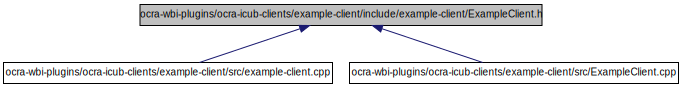
\includegraphics[width=350pt]{ExampleClient_8h__dep__incl}
\end{center}
\end{figure}
\subsection*{\-Classes}
\begin{DoxyCompactItemize}
\item 
class \hyperlink{classExampleClient}{\-Example\-Client}
\end{DoxyCompactItemize}

\hypertarget{example-client_8cpp}{\section{ocra-\/wbi-\/plugins/ocra-\/icub-\/clients/example-\/client/src/example-\/client.cpp \-File \-Reference}
\label{example-client_8cpp}\index{ocra-\/wbi-\/plugins/ocra-\/icub-\/clients/example-\/client/src/example-\/client.\-cpp@{ocra-\/wbi-\/plugins/ocra-\/icub-\/clients/example-\/client/src/example-\/client.\-cpp}}
}
{\ttfamily \#include $<$yarp/os/\-Resource\-Finder.\-h$>$}\*
{\ttfamily \#include $<$yarp/os/\-Network.\-h$>$}\*
{\ttfamily \#include $<$yarp/os/\-Log.\-h$>$}\*
{\ttfamily \#include $<$yarp/os/\-Log\-Stream.\-h$>$}\*
{\ttfamily \#include $<$yarp/os/\-Time.\-h$>$}\*
{\ttfamily \#include \char`\"{}example-\/client/\-Example\-Client.\-h\char`\"{}}\*
{\ttfamily \#include $<$ocra-\/icub/\-Icub\-Client.\-h$>$}\*
{\ttfamily \#include $<$ocra-\/recipes/\-Controller\-Client.\-h$>$}\*
{\ttfamily \#include $<$ocra-\/recipes/\-Client\-Manager.\-h$>$}\*
\-Include dependency graph for example-\/client.cpp\-:\nopagebreak
\begin{figure}[H]
\begin{center}
\leavevmode
\includegraphics[width=350pt]{example-client_8cpp__incl}
\end{center}
\end{figure}
\subsection*{\-Functions}
\begin{DoxyCompactItemize}
\item 
int \hyperlink{example-client_8cpp_a0ddf1224851353fc92bfbff6f499fa97}{main} (int argc, char $\ast$argv\mbox{[}$\,$\mbox{]})
\end{DoxyCompactItemize}


\subsection{\-Detailed \-Description}
\begin{DoxyAuthor}{\-Author}
\mbox{[}\-Ryan \-Lober\mbox{]}(\href{http://www.ryanlober.com}{\tt http\-://www.\-ryanlober.\-com}) 

\mbox{[}\-Antoine \-Hoarau\mbox{]}(\href{http://ahoarau.github.io}{\tt http\-://ahoarau.\-github.\-io}) 
\end{DoxyAuthor}
\begin{DoxyDate}{\-Date}
\-Feb 2016 
\end{DoxyDate}
\begin{DoxyCopyright}{\-Copyright}
\-G\-N\-U \-General \-Public \-License. 
\end{DoxyCopyright}


\subsection{\-Function \-Documentation}
\hypertarget{example-client_8cpp_a0ddf1224851353fc92bfbff6f499fa97}{\index{example-\/client.\-cpp@{example-\/client.\-cpp}!main@{main}}
\index{main@{main}!example-client.cpp@{example-\/client.\-cpp}}
\subsubsection[{main}]{\setlength{\rightskip}{0pt plus 5cm}int {\bf main} (
\begin{DoxyParamCaption}
\item[{int}]{argc, }
\item[{char $\ast$}]{argv\mbox{[}$\,$\mbox{]}}
\end{DoxyParamCaption}
)}}\label{example-client_8cpp_a0ddf1224851353fc92bfbff6f499fa97}

\hypertarget{ExampleClient_8cpp}{\section{ocra-\/wbi-\/plugins/ocra-\/icub-\/clients/example-\/client/src/\-Example\-Client.cpp \-File \-Reference}
\label{ExampleClient_8cpp}\index{ocra-\/wbi-\/plugins/ocra-\/icub-\/clients/example-\/client/src/\-Example\-Client.\-cpp@{ocra-\/wbi-\/plugins/ocra-\/icub-\/clients/example-\/client/src/\-Example\-Client.\-cpp}}
}
{\ttfamily \#include \char`\"{}example-\/client/\-Example\-Client.\-h\char`\"{}}\*
\-Include dependency graph for \-Example\-Client.\-cpp\-:
\nopagebreak
\begin{figure}[H]
\begin{center}
\leavevmode
\includegraphics[width=350pt]{ExampleClient_8cpp__incl}
\end{center}
\end{figure}

\hypertarget{SittingDemoClient_8h}{\section{ocra-\/wbi-\/plugins/ocra-\/icub-\/clients/sitting-\/demo/include/sitting-\/demo/\-Sitting\-Demo\-Client.h \-File \-Reference}
\label{SittingDemoClient_8h}\index{ocra-\/wbi-\/plugins/ocra-\/icub-\/clients/sitting-\/demo/include/sitting-\/demo/\-Sitting\-Demo\-Client.\-h@{ocra-\/wbi-\/plugins/ocra-\/icub-\/clients/sitting-\/demo/include/sitting-\/demo/\-Sitting\-Demo\-Client.\-h}}
}
{\ttfamily \#include $<$ocra-\/icub/\-Icub\-Client.\-h$>$}\*
{\ttfamily \#include $<$ocra-\/recipes/\-Trajectory\-Thread.\-h$>$}\*
{\ttfamily \#include $<$ocra-\/recipes/\-Controller\-Client.\-h$>$}\*
\-Include dependency graph for \-Sitting\-Demo\-Client.\-h\-:
\nopagebreak
\begin{figure}[H]
\begin{center}
\leavevmode
\includegraphics[width=350pt]{SittingDemoClient_8h__incl}
\end{center}
\end{figure}
\-This graph shows which files directly or indirectly include this file\-:
\nopagebreak
\begin{figure}[H]
\begin{center}
\leavevmode
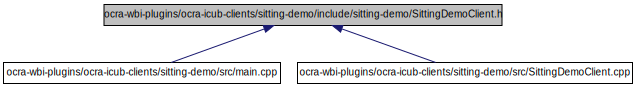
\includegraphics[width=350pt]{SittingDemoClient_8h__dep__incl}
\end{center}
\end{figure}
\subsection*{\-Classes}
\begin{DoxyCompactItemize}
\item 
class \hyperlink{classSittingDemoClient}{\-Sitting\-Demo\-Client}
\end{DoxyCompactItemize}

\hypertarget{SittingDemoClient_8cpp}{\section{ocra-\/wbi-\/plugins/ocra-\/icub-\/clients/sitting-\/demo/src/\-Sitting\-Demo\-Client.cpp \-File \-Reference}
\label{SittingDemoClient_8cpp}\index{ocra-\/wbi-\/plugins/ocra-\/icub-\/clients/sitting-\/demo/src/\-Sitting\-Demo\-Client.\-cpp@{ocra-\/wbi-\/plugins/ocra-\/icub-\/clients/sitting-\/demo/src/\-Sitting\-Demo\-Client.\-cpp}}
}
{\ttfamily \#include \char`\"{}sitting-\/demo/\-Sitting\-Demo\-Client.\-h\char`\"{}}\*
\-Include dependency graph for \-Sitting\-Demo\-Client.\-cpp\-:
\nopagebreak
\begin{figure}[H]
\begin{center}
\leavevmode
\includegraphics[width=350pt]{SittingDemoClient_8cpp__incl}
\end{center}
\end{figure}

\hypertarget{StandingDemoClient_8h}{\section{ocra-\/wbi-\/plugins/ocra-\/icub-\/clients/standing-\/demo/include/standing-\/demo/\-Standing\-Demo\-Client.h \-File \-Reference}
\label{StandingDemoClient_8h}\index{ocra-\/wbi-\/plugins/ocra-\/icub-\/clients/standing-\/demo/include/standing-\/demo/\-Standing\-Demo\-Client.\-h@{ocra-\/wbi-\/plugins/ocra-\/icub-\/clients/standing-\/demo/include/standing-\/demo/\-Standing\-Demo\-Client.\-h}}
}
{\ttfamily \#include $<$ocra-\/icub/\-Icub\-Client.\-h$>$}\*
{\ttfamily \#include $<$ocra-\/recipes/\-Trajectory\-Thread.\-h$>$}\*
{\ttfamily \#include $<$ocra-\/recipes/\-Controller\-Client.\-h$>$}\*
\-Include dependency graph for \-Standing\-Demo\-Client.\-h\-:
\nopagebreak
\begin{figure}[H]
\begin{center}
\leavevmode
\includegraphics[width=350pt]{StandingDemoClient_8h__incl}
\end{center}
\end{figure}
\-This graph shows which files directly or indirectly include this file\-:
\nopagebreak
\begin{figure}[H]
\begin{center}
\leavevmode
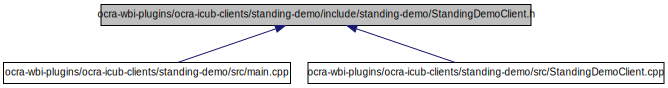
\includegraphics[width=350pt]{StandingDemoClient_8h__dep__incl}
\end{center}
\end{figure}
\subsection*{\-Classes}
\begin{DoxyCompactItemize}
\item 
class \hyperlink{classStandingDemoClient}{\-Standing\-Demo\-Client}
\end{DoxyCompactItemize}

\hypertarget{StandingDemoClient_8cpp}{\section{ocra-\/wbi-\/plugins/ocra-\/icub-\/clients/standing-\/demo/src/\-Standing\-Demo\-Client.cpp \-File \-Reference}
\label{StandingDemoClient_8cpp}\index{ocra-\/wbi-\/plugins/ocra-\/icub-\/clients/standing-\/demo/src/\-Standing\-Demo\-Client.\-cpp@{ocra-\/wbi-\/plugins/ocra-\/icub-\/clients/standing-\/demo/src/\-Standing\-Demo\-Client.\-cpp}}
}
{\ttfamily \#include \char`\"{}standing-\/demo/\-Standing\-Demo\-Client.\-h\char`\"{}}\*
\-Include dependency graph for \-Standing\-Demo\-Client.\-cpp\-:
\nopagebreak
\begin{figure}[H]
\begin{center}
\leavevmode
\includegraphics[width=350pt]{StandingDemoClient_8cpp__incl}
\end{center}
\end{figure}

\hypertarget{SteppingDemoClient_8h}{\section{ocra-\/wbi-\/plugins/ocra-\/icub-\/clients/stepping-\/demo/include/stepping-\/demo/\-Stepping\-Demo\-Client.h \-File \-Reference}
\label{SteppingDemoClient_8h}\index{ocra-\/wbi-\/plugins/ocra-\/icub-\/clients/stepping-\/demo/include/stepping-\/demo/\-Stepping\-Demo\-Client.\-h@{ocra-\/wbi-\/plugins/ocra-\/icub-\/clients/stepping-\/demo/include/stepping-\/demo/\-Stepping\-Demo\-Client.\-h}}
}
{\ttfamily \#include $<$ocra-\/icub/\-Icub\-Client.\-h$>$}\*
{\ttfamily \#include $<$ocra-\/recipes/\-Trajectory\-Thread.\-h$>$}\*
{\ttfamily \#include $<$ocra-\/recipes/\-Controller\-Client.\-h$>$}\*
{\ttfamily \#include $<$ocra/util/\-Errors\-Helper.\-h$>$}\*
\-Include dependency graph for \-Stepping\-Demo\-Client.\-h\-:\nopagebreak
\begin{figure}[H]
\begin{center}
\leavevmode
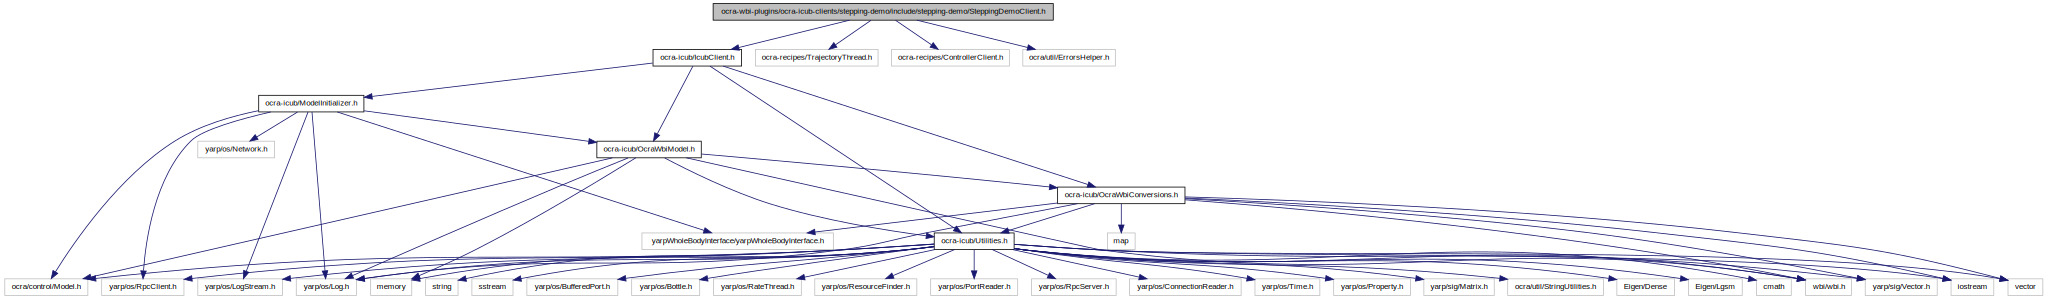
\includegraphics[width=350pt]{SteppingDemoClient_8h__incl}
\end{center}
\end{figure}
\-This graph shows which files directly or indirectly include this file\-:\nopagebreak
\begin{figure}[H]
\begin{center}
\leavevmode
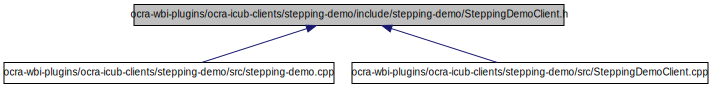
\includegraphics[width=350pt]{SteppingDemoClient_8h__dep__incl}
\end{center}
\end{figure}
\subsection*{\-Classes}
\begin{DoxyCompactItemize}
\item 
struct \hyperlink{structWalkingParams}{\-Walking\-Params}
\item 
class \hyperlink{classSteppingDemoClient}{\-Stepping\-Demo\-Client}
\end{DoxyCompactItemize}
\subsection*{\-Enumerations}
\begin{DoxyCompactItemize}
\item 
enum \hyperlink{SteppingDemoClient_8h_ac0c3848a609566394821d9826e0fdd5b}{\-C\-O\-M\-\_\-\-S\-U\-P\-P\-O\-R\-T\-\_\-\-P\-O\-S\-I\-T\-I\-O\-N} \{ \hyperlink{SteppingDemoClient_8h_ac0c3848a609566394821d9826e0fdd5ba07cd79ee915be269a43f655f31cd3ccf}{\-L\-E\-F\-T\-\_\-\-F\-O\-O\-T\-\_\-\-X\-Y}, 
\hyperlink{SteppingDemoClient_8h_ac0c3848a609566394821d9826e0fdd5ba273605381ab0231d2abb4a8096faabfd}{\-R\-I\-G\-H\-T\-\_\-\-F\-O\-O\-T\-\_\-\-X\-Y}, 
\hyperlink{SteppingDemoClient_8h_ac0c3848a609566394821d9826e0fdd5bad32a9ea5bb598218529abf1a5b9b50cf}{\-C\-E\-N\-T\-E\-R\-E\-D\-\_\-\-B\-E\-T\-W\-E\-E\-N\-\_\-\-F\-E\-E\-T\-\_\-\-X\-Y}
 \}
\item 
enum \hyperlink{SteppingDemoClient_8h_af2a8507bf21c3ce9b0e67a23381251c6}{\-C\-O\-N\-T\-R\-O\-L\-\_\-\-P\-H\-A\-S\-E} \{ \hyperlink{SteppingDemoClient_8h_af2a8507bf21c3ce9b0e67a23381251c6afe7fc4a2f5d6778bbb96f412be37d63c}{\-M\-O\-V\-E\-\_\-\-T\-O\-\_\-\-L\-E\-F\-T\-\_\-\-S\-U\-P\-P\-O\-R\-T}, 
\hyperlink{SteppingDemoClient_8h_af2a8507bf21c3ce9b0e67a23381251c6a3b4335037acf972dd5d60348ca20d394}{\-M\-O\-V\-E\-\_\-\-T\-O\-\_\-\-R\-I\-G\-H\-T\-\_\-\-S\-U\-P\-P\-O\-R\-T}, 
\hyperlink{SteppingDemoClient_8h_af2a8507bf21c3ce9b0e67a23381251c6a362d8557e44bcc19f6b4d9096bb54401}{\-M\-O\-V\-E\-\_\-\-T\-O\-\_\-\-D\-O\-U\-B\-L\-E\-\_\-\-S\-U\-P\-P\-O\-R\-T}, 
\hyperlink{SteppingDemoClient_8h_af2a8507bf21c3ce9b0e67a23381251c6a4ff6c6ae9503ea4bca745c7d7819523e}{\-S\-T\-E\-P\-\_\-\-F\-O\-R\-W\-A\-R\-D}
 \}
\item 
enum \hyperlink{SteppingDemoClient_8h_ab0673d7f17cdd57b8fa124abb330287f}{\-F\-O\-O\-T\-\_\-\-C\-O\-N\-T\-A\-C\-T\-S} \{ \hyperlink{SteppingDemoClient_8h_ab0673d7f17cdd57b8fa124abb330287fa7760daad9db1ede8c57b06189deca9f3}{\-L\-E\-F\-T\-\_\-\-F\-O\-O\-T}, 
\hyperlink{SteppingDemoClient_8h_ab0673d7f17cdd57b8fa124abb330287face119c66af60ac0781b137aa87d7be62}{\-R\-I\-G\-H\-T\-\_\-\-F\-O\-O\-T}
 \}
\item 
enum \hyperlink{SteppingDemoClient_8h_abd6d177d63e98aa1b4ed4b8329e2a379}{\-M\-O\-T\-I\-O\-N\-\_\-\-T\-Y\-P\-E} \{ \hyperlink{SteppingDemoClient_8h_abd6d177d63e98aa1b4ed4b8329e2a379a55b57dce74f14a62104ae66e62789eb3}{\-L\-E\-F\-T\-\_\-\-T\-O\-\_\-\-R\-I\-G\-H\-T}, 
\hyperlink{SteppingDemoClient_8h_abd6d177d63e98aa1b4ed4b8329e2a379ada7017955bb1db9f0954017358028fa6}{\-S\-T\-A\-T\-I\-C\-\_\-\-W\-A\-L\-K\-I\-N\-G}
 \}
\end{DoxyCompactItemize}


\subsection{\-Enumeration \-Type \-Documentation}
\hypertarget{SteppingDemoClient_8h_ac0c3848a609566394821d9826e0fdd5b}{\index{\-Stepping\-Demo\-Client.\-h@{\-Stepping\-Demo\-Client.\-h}!\-C\-O\-M\-\_\-\-S\-U\-P\-P\-O\-R\-T\-\_\-\-P\-O\-S\-I\-T\-I\-O\-N@{\-C\-O\-M\-\_\-\-S\-U\-P\-P\-O\-R\-T\-\_\-\-P\-O\-S\-I\-T\-I\-O\-N}}
\index{\-C\-O\-M\-\_\-\-S\-U\-P\-P\-O\-R\-T\-\_\-\-P\-O\-S\-I\-T\-I\-O\-N@{\-C\-O\-M\-\_\-\-S\-U\-P\-P\-O\-R\-T\-\_\-\-P\-O\-S\-I\-T\-I\-O\-N}!SteppingDemoClient.h@{\-Stepping\-Demo\-Client.\-h}}
\subsubsection[{\-C\-O\-M\-\_\-\-S\-U\-P\-P\-O\-R\-T\-\_\-\-P\-O\-S\-I\-T\-I\-O\-N}]{\setlength{\rightskip}{0pt plus 5cm}enum {\bf \-C\-O\-M\-\_\-\-S\-U\-P\-P\-O\-R\-T\-\_\-\-P\-O\-S\-I\-T\-I\-O\-N}}}\label{SteppingDemoClient_8h_ac0c3848a609566394821d9826e0fdd5b}
\begin{Desc}
\item[\-Enumerator\-: ]\par
\begin{description}
\index{\-L\-E\-F\-T\-\_\-\-F\-O\-O\-T\-\_\-\-X\-Y@{\-L\-E\-F\-T\-\_\-\-F\-O\-O\-T\-\_\-\-X\-Y}!\-Stepping\-Demo\-Client.\-h@{\-Stepping\-Demo\-Client.\-h}}\index{\-Stepping\-Demo\-Client.\-h@{\-Stepping\-Demo\-Client.\-h}!\-L\-E\-F\-T\-\_\-\-F\-O\-O\-T\-\_\-\-X\-Y@{\-L\-E\-F\-T\-\_\-\-F\-O\-O\-T\-\_\-\-X\-Y}}\item[{\em 
\hypertarget{SteppingDemoClient_8h_ac0c3848a609566394821d9826e0fdd5ba07cd79ee915be269a43f655f31cd3ccf}{\-L\-E\-F\-T\-\_\-\-F\-O\-O\-T\-\_\-\-X\-Y}\label{SteppingDemoClient_8h_ac0c3848a609566394821d9826e0fdd5ba07cd79ee915be269a43f655f31cd3ccf}
}]\index{\-R\-I\-G\-H\-T\-\_\-\-F\-O\-O\-T\-\_\-\-X\-Y@{\-R\-I\-G\-H\-T\-\_\-\-F\-O\-O\-T\-\_\-\-X\-Y}!\-Stepping\-Demo\-Client.\-h@{\-Stepping\-Demo\-Client.\-h}}\index{\-Stepping\-Demo\-Client.\-h@{\-Stepping\-Demo\-Client.\-h}!\-R\-I\-G\-H\-T\-\_\-\-F\-O\-O\-T\-\_\-\-X\-Y@{\-R\-I\-G\-H\-T\-\_\-\-F\-O\-O\-T\-\_\-\-X\-Y}}\item[{\em 
\hypertarget{SteppingDemoClient_8h_ac0c3848a609566394821d9826e0fdd5ba273605381ab0231d2abb4a8096faabfd}{\-R\-I\-G\-H\-T\-\_\-\-F\-O\-O\-T\-\_\-\-X\-Y}\label{SteppingDemoClient_8h_ac0c3848a609566394821d9826e0fdd5ba273605381ab0231d2abb4a8096faabfd}
}]\index{\-C\-E\-N\-T\-E\-R\-E\-D\-\_\-\-B\-E\-T\-W\-E\-E\-N\-\_\-\-F\-E\-E\-T\-\_\-\-X\-Y@{\-C\-E\-N\-T\-E\-R\-E\-D\-\_\-\-B\-E\-T\-W\-E\-E\-N\-\_\-\-F\-E\-E\-T\-\_\-\-X\-Y}!\-Stepping\-Demo\-Client.\-h@{\-Stepping\-Demo\-Client.\-h}}\index{\-Stepping\-Demo\-Client.\-h@{\-Stepping\-Demo\-Client.\-h}!\-C\-E\-N\-T\-E\-R\-E\-D\-\_\-\-B\-E\-T\-W\-E\-E\-N\-\_\-\-F\-E\-E\-T\-\_\-\-X\-Y@{\-C\-E\-N\-T\-E\-R\-E\-D\-\_\-\-B\-E\-T\-W\-E\-E\-N\-\_\-\-F\-E\-E\-T\-\_\-\-X\-Y}}\item[{\em 
\hypertarget{SteppingDemoClient_8h_ac0c3848a609566394821d9826e0fdd5bad32a9ea5bb598218529abf1a5b9b50cf}{\-C\-E\-N\-T\-E\-R\-E\-D\-\_\-\-B\-E\-T\-W\-E\-E\-N\-\_\-\-F\-E\-E\-T\-\_\-\-X\-Y}\label{SteppingDemoClient_8h_ac0c3848a609566394821d9826e0fdd5bad32a9ea5bb598218529abf1a5b9b50cf}
}]\end{description}
\end{Desc}

\hypertarget{SteppingDemoClient_8h_af2a8507bf21c3ce9b0e67a23381251c6}{\index{\-Stepping\-Demo\-Client.\-h@{\-Stepping\-Demo\-Client.\-h}!\-C\-O\-N\-T\-R\-O\-L\-\_\-\-P\-H\-A\-S\-E@{\-C\-O\-N\-T\-R\-O\-L\-\_\-\-P\-H\-A\-S\-E}}
\index{\-C\-O\-N\-T\-R\-O\-L\-\_\-\-P\-H\-A\-S\-E@{\-C\-O\-N\-T\-R\-O\-L\-\_\-\-P\-H\-A\-S\-E}!SteppingDemoClient.h@{\-Stepping\-Demo\-Client.\-h}}
\subsubsection[{\-C\-O\-N\-T\-R\-O\-L\-\_\-\-P\-H\-A\-S\-E}]{\setlength{\rightskip}{0pt plus 5cm}enum {\bf \-C\-O\-N\-T\-R\-O\-L\-\_\-\-P\-H\-A\-S\-E}}}\label{SteppingDemoClient_8h_af2a8507bf21c3ce9b0e67a23381251c6}
\begin{Desc}
\item[\-Enumerator\-: ]\par
\begin{description}
\index{\-M\-O\-V\-E\-\_\-\-T\-O\-\_\-\-L\-E\-F\-T\-\_\-\-S\-U\-P\-P\-O\-R\-T@{\-M\-O\-V\-E\-\_\-\-T\-O\-\_\-\-L\-E\-F\-T\-\_\-\-S\-U\-P\-P\-O\-R\-T}!\-Stepping\-Demo\-Client.\-h@{\-Stepping\-Demo\-Client.\-h}}\index{\-Stepping\-Demo\-Client.\-h@{\-Stepping\-Demo\-Client.\-h}!\-M\-O\-V\-E\-\_\-\-T\-O\-\_\-\-L\-E\-F\-T\-\_\-\-S\-U\-P\-P\-O\-R\-T@{\-M\-O\-V\-E\-\_\-\-T\-O\-\_\-\-L\-E\-F\-T\-\_\-\-S\-U\-P\-P\-O\-R\-T}}\item[{\em 
\hypertarget{SteppingDemoClient_8h_af2a8507bf21c3ce9b0e67a23381251c6afe7fc4a2f5d6778bbb96f412be37d63c}{\-M\-O\-V\-E\-\_\-\-T\-O\-\_\-\-L\-E\-F\-T\-\_\-\-S\-U\-P\-P\-O\-R\-T}\label{SteppingDemoClient_8h_af2a8507bf21c3ce9b0e67a23381251c6afe7fc4a2f5d6778bbb96f412be37d63c}
}]\index{\-M\-O\-V\-E\-\_\-\-T\-O\-\_\-\-R\-I\-G\-H\-T\-\_\-\-S\-U\-P\-P\-O\-R\-T@{\-M\-O\-V\-E\-\_\-\-T\-O\-\_\-\-R\-I\-G\-H\-T\-\_\-\-S\-U\-P\-P\-O\-R\-T}!\-Stepping\-Demo\-Client.\-h@{\-Stepping\-Demo\-Client.\-h}}\index{\-Stepping\-Demo\-Client.\-h@{\-Stepping\-Demo\-Client.\-h}!\-M\-O\-V\-E\-\_\-\-T\-O\-\_\-\-R\-I\-G\-H\-T\-\_\-\-S\-U\-P\-P\-O\-R\-T@{\-M\-O\-V\-E\-\_\-\-T\-O\-\_\-\-R\-I\-G\-H\-T\-\_\-\-S\-U\-P\-P\-O\-R\-T}}\item[{\em 
\hypertarget{SteppingDemoClient_8h_af2a8507bf21c3ce9b0e67a23381251c6a3b4335037acf972dd5d60348ca20d394}{\-M\-O\-V\-E\-\_\-\-T\-O\-\_\-\-R\-I\-G\-H\-T\-\_\-\-S\-U\-P\-P\-O\-R\-T}\label{SteppingDemoClient_8h_af2a8507bf21c3ce9b0e67a23381251c6a3b4335037acf972dd5d60348ca20d394}
}]\index{\-M\-O\-V\-E\-\_\-\-T\-O\-\_\-\-D\-O\-U\-B\-L\-E\-\_\-\-S\-U\-P\-P\-O\-R\-T@{\-M\-O\-V\-E\-\_\-\-T\-O\-\_\-\-D\-O\-U\-B\-L\-E\-\_\-\-S\-U\-P\-P\-O\-R\-T}!\-Stepping\-Demo\-Client.\-h@{\-Stepping\-Demo\-Client.\-h}}\index{\-Stepping\-Demo\-Client.\-h@{\-Stepping\-Demo\-Client.\-h}!\-M\-O\-V\-E\-\_\-\-T\-O\-\_\-\-D\-O\-U\-B\-L\-E\-\_\-\-S\-U\-P\-P\-O\-R\-T@{\-M\-O\-V\-E\-\_\-\-T\-O\-\_\-\-D\-O\-U\-B\-L\-E\-\_\-\-S\-U\-P\-P\-O\-R\-T}}\item[{\em 
\hypertarget{SteppingDemoClient_8h_af2a8507bf21c3ce9b0e67a23381251c6a362d8557e44bcc19f6b4d9096bb54401}{\-M\-O\-V\-E\-\_\-\-T\-O\-\_\-\-D\-O\-U\-B\-L\-E\-\_\-\-S\-U\-P\-P\-O\-R\-T}\label{SteppingDemoClient_8h_af2a8507bf21c3ce9b0e67a23381251c6a362d8557e44bcc19f6b4d9096bb54401}
}]\index{\-S\-T\-E\-P\-\_\-\-F\-O\-R\-W\-A\-R\-D@{\-S\-T\-E\-P\-\_\-\-F\-O\-R\-W\-A\-R\-D}!\-Stepping\-Demo\-Client.\-h@{\-Stepping\-Demo\-Client.\-h}}\index{\-Stepping\-Demo\-Client.\-h@{\-Stepping\-Demo\-Client.\-h}!\-S\-T\-E\-P\-\_\-\-F\-O\-R\-W\-A\-R\-D@{\-S\-T\-E\-P\-\_\-\-F\-O\-R\-W\-A\-R\-D}}\item[{\em 
\hypertarget{SteppingDemoClient_8h_af2a8507bf21c3ce9b0e67a23381251c6a4ff6c6ae9503ea4bca745c7d7819523e}{\-S\-T\-E\-P\-\_\-\-F\-O\-R\-W\-A\-R\-D}\label{SteppingDemoClient_8h_af2a8507bf21c3ce9b0e67a23381251c6a4ff6c6ae9503ea4bca745c7d7819523e}
}]\end{description}
\end{Desc}

\hypertarget{SteppingDemoClient_8h_ab0673d7f17cdd57b8fa124abb330287f}{\index{\-Stepping\-Demo\-Client.\-h@{\-Stepping\-Demo\-Client.\-h}!\-F\-O\-O\-T\-\_\-\-C\-O\-N\-T\-A\-C\-T\-S@{\-F\-O\-O\-T\-\_\-\-C\-O\-N\-T\-A\-C\-T\-S}}
\index{\-F\-O\-O\-T\-\_\-\-C\-O\-N\-T\-A\-C\-T\-S@{\-F\-O\-O\-T\-\_\-\-C\-O\-N\-T\-A\-C\-T\-S}!SteppingDemoClient.h@{\-Stepping\-Demo\-Client.\-h}}
\subsubsection[{\-F\-O\-O\-T\-\_\-\-C\-O\-N\-T\-A\-C\-T\-S}]{\setlength{\rightskip}{0pt plus 5cm}enum {\bf \-F\-O\-O\-T\-\_\-\-C\-O\-N\-T\-A\-C\-T\-S}}}\label{SteppingDemoClient_8h_ab0673d7f17cdd57b8fa124abb330287f}
\begin{Desc}
\item[\-Enumerator\-: ]\par
\begin{description}
\index{\-L\-E\-F\-T\-\_\-\-F\-O\-O\-T@{\-L\-E\-F\-T\-\_\-\-F\-O\-O\-T}!\-Stepping\-Demo\-Client.\-h@{\-Stepping\-Demo\-Client.\-h}}\index{\-Stepping\-Demo\-Client.\-h@{\-Stepping\-Demo\-Client.\-h}!\-L\-E\-F\-T\-\_\-\-F\-O\-O\-T@{\-L\-E\-F\-T\-\_\-\-F\-O\-O\-T}}\item[{\em 
\hypertarget{SteppingDemoClient_8h_ab0673d7f17cdd57b8fa124abb330287fa7760daad9db1ede8c57b06189deca9f3}{\-L\-E\-F\-T\-\_\-\-F\-O\-O\-T}\label{SteppingDemoClient_8h_ab0673d7f17cdd57b8fa124abb330287fa7760daad9db1ede8c57b06189deca9f3}
}]\index{\-R\-I\-G\-H\-T\-\_\-\-F\-O\-O\-T@{\-R\-I\-G\-H\-T\-\_\-\-F\-O\-O\-T}!\-Stepping\-Demo\-Client.\-h@{\-Stepping\-Demo\-Client.\-h}}\index{\-Stepping\-Demo\-Client.\-h@{\-Stepping\-Demo\-Client.\-h}!\-R\-I\-G\-H\-T\-\_\-\-F\-O\-O\-T@{\-R\-I\-G\-H\-T\-\_\-\-F\-O\-O\-T}}\item[{\em 
\hypertarget{SteppingDemoClient_8h_ab0673d7f17cdd57b8fa124abb330287face119c66af60ac0781b137aa87d7be62}{\-R\-I\-G\-H\-T\-\_\-\-F\-O\-O\-T}\label{SteppingDemoClient_8h_ab0673d7f17cdd57b8fa124abb330287face119c66af60ac0781b137aa87d7be62}
}]\end{description}
\end{Desc}

\hypertarget{SteppingDemoClient_8h_abd6d177d63e98aa1b4ed4b8329e2a379}{\index{\-Stepping\-Demo\-Client.\-h@{\-Stepping\-Demo\-Client.\-h}!\-M\-O\-T\-I\-O\-N\-\_\-\-T\-Y\-P\-E@{\-M\-O\-T\-I\-O\-N\-\_\-\-T\-Y\-P\-E}}
\index{\-M\-O\-T\-I\-O\-N\-\_\-\-T\-Y\-P\-E@{\-M\-O\-T\-I\-O\-N\-\_\-\-T\-Y\-P\-E}!SteppingDemoClient.h@{\-Stepping\-Demo\-Client.\-h}}
\subsubsection[{\-M\-O\-T\-I\-O\-N\-\_\-\-T\-Y\-P\-E}]{\setlength{\rightskip}{0pt plus 5cm}enum {\bf \-M\-O\-T\-I\-O\-N\-\_\-\-T\-Y\-P\-E}}}\label{SteppingDemoClient_8h_abd6d177d63e98aa1b4ed4b8329e2a379}
\begin{Desc}
\item[\-Enumerator\-: ]\par
\begin{description}
\index{\-L\-E\-F\-T\-\_\-\-T\-O\-\_\-\-R\-I\-G\-H\-T@{\-L\-E\-F\-T\-\_\-\-T\-O\-\_\-\-R\-I\-G\-H\-T}!\-Stepping\-Demo\-Client.\-h@{\-Stepping\-Demo\-Client.\-h}}\index{\-Stepping\-Demo\-Client.\-h@{\-Stepping\-Demo\-Client.\-h}!\-L\-E\-F\-T\-\_\-\-T\-O\-\_\-\-R\-I\-G\-H\-T@{\-L\-E\-F\-T\-\_\-\-T\-O\-\_\-\-R\-I\-G\-H\-T}}\item[{\em 
\hypertarget{SteppingDemoClient_8h_abd6d177d63e98aa1b4ed4b8329e2a379a55b57dce74f14a62104ae66e62789eb3}{\-L\-E\-F\-T\-\_\-\-T\-O\-\_\-\-R\-I\-G\-H\-T}\label{SteppingDemoClient_8h_abd6d177d63e98aa1b4ed4b8329e2a379a55b57dce74f14a62104ae66e62789eb3}
}]\index{\-S\-T\-A\-T\-I\-C\-\_\-\-W\-A\-L\-K\-I\-N\-G@{\-S\-T\-A\-T\-I\-C\-\_\-\-W\-A\-L\-K\-I\-N\-G}!\-Stepping\-Demo\-Client.\-h@{\-Stepping\-Demo\-Client.\-h}}\index{\-Stepping\-Demo\-Client.\-h@{\-Stepping\-Demo\-Client.\-h}!\-S\-T\-A\-T\-I\-C\-\_\-\-W\-A\-L\-K\-I\-N\-G@{\-S\-T\-A\-T\-I\-C\-\_\-\-W\-A\-L\-K\-I\-N\-G}}\item[{\em 
\hypertarget{SteppingDemoClient_8h_abd6d177d63e98aa1b4ed4b8329e2a379ada7017955bb1db9f0954017358028fa6}{\-S\-T\-A\-T\-I\-C\-\_\-\-W\-A\-L\-K\-I\-N\-G}\label{SteppingDemoClient_8h_abd6d177d63e98aa1b4ed4b8329e2a379ada7017955bb1db9f0954017358028fa6}
}]\end{description}
\end{Desc}


\hypertarget{stepping-demo_8cpp}{\section{ocra-\/wbi-\/plugins/ocra-\/icub-\/clients/stepping-\/demo/src/stepping-\/demo.cpp \-File \-Reference}
\label{stepping-demo_8cpp}\index{ocra-\/wbi-\/plugins/ocra-\/icub-\/clients/stepping-\/demo/src/stepping-\/demo.\-cpp@{ocra-\/wbi-\/plugins/ocra-\/icub-\/clients/stepping-\/demo/src/stepping-\/demo.\-cpp}}
}
{\ttfamily \#include $<$yarp/os/\-Resource\-Finder.\-h$>$}\*
{\ttfamily \#include $<$yarp/os/\-Network.\-h$>$}\*
{\ttfamily \#include $<$yarp/os/\-Log.\-h$>$}\*
{\ttfamily \#include $<$yarp/os/\-Log\-Stream.\-h$>$}\*
{\ttfamily \#include $<$yarp/os/\-Time.\-h$>$}\*
{\ttfamily \#include \char`\"{}stepping-\/demo/\-Stepping\-Demo\-Client.\-h\char`\"{}}\*
{\ttfamily \#include $<$ocra-\/icub/\-Icub\-Client.\-h$>$}\*
{\ttfamily \#include $<$ocra-\/recipes/\-Controller\-Client.\-h$>$}\*
{\ttfamily \#include $<$ocra-\/recipes/\-Client\-Manager.\-h$>$}\*
\-Include dependency graph for stepping-\/demo.cpp\-:
\nopagebreak
\begin{figure}[H]
\begin{center}
\leavevmode
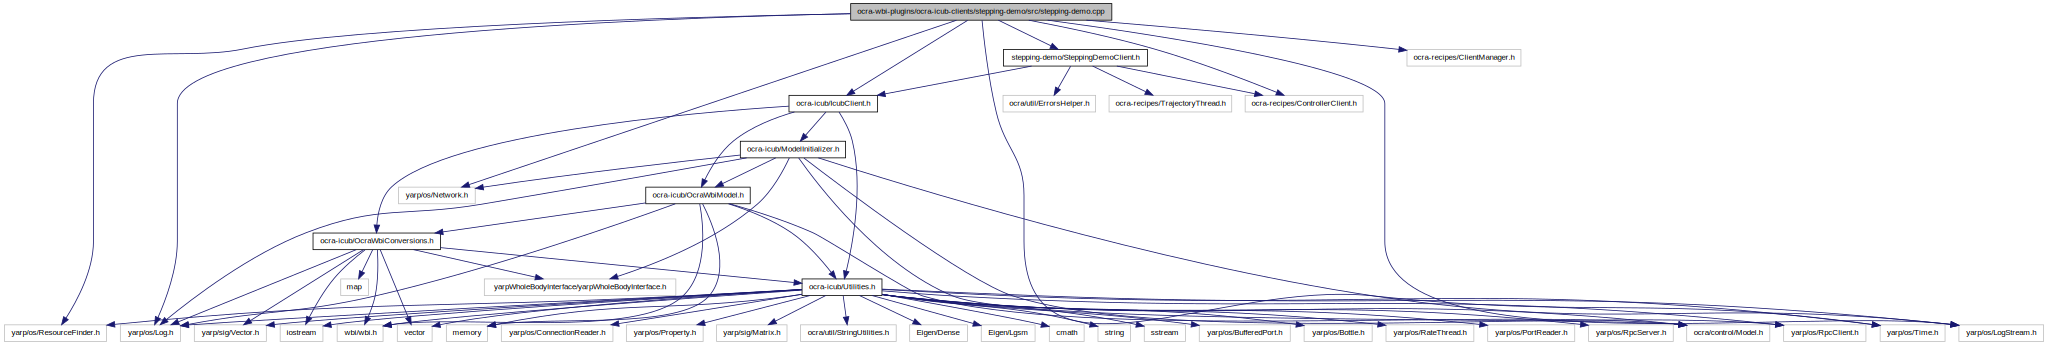
\includegraphics[width=350pt]{stepping-demo_8cpp__incl}
\end{center}
\end{figure}
\subsection*{\-Functions}
\begin{DoxyCompactItemize}
\item 
int \hyperlink{stepping-demo_8cpp_a0ddf1224851353fc92bfbff6f499fa97}{main} (int argc, char $\ast$argv\mbox{[}$\,$\mbox{]})
\end{DoxyCompactItemize}


\subsection{\-Detailed \-Description}
\begin{DoxyAuthor}{\-Author}
\mbox{[}\-Ryan \-Lober\mbox{]}(\href{http://www.ryanlober.com}{\tt http\-://www.\-ryanlober.\-com}) 

\mbox{[}\-Antoine \-Hoarau\mbox{]}(\href{http://ahoarau.github.io}{\tt http\-://ahoarau.\-github.\-io}) 
\end{DoxyAuthor}
\begin{DoxyDate}{\-Date}
\-Feb 2016 
\end{DoxyDate}
\begin{DoxyCopyright}{\-Copyright}
\-G\-N\-U \-General \-Public \-License. 
\end{DoxyCopyright}


\subsection{\-Function \-Documentation}
\hypertarget{stepping-demo_8cpp_a0ddf1224851353fc92bfbff6f499fa97}{\index{stepping-\/demo.\-cpp@{stepping-\/demo.\-cpp}!main@{main}}
\index{main@{main}!stepping-demo.cpp@{stepping-\/demo.\-cpp}}
\subsubsection[{main}]{\setlength{\rightskip}{0pt plus 5cm}int {\bf main} (
\begin{DoxyParamCaption}
\item[{int}]{argc, }
\item[{char $\ast$}]{argv\mbox{[}$\,$\mbox{]}}
\end{DoxyParamCaption}
)}}\label{stepping-demo_8cpp_a0ddf1224851353fc92bfbff6f499fa97}

\input{SteppingDemoClient_8cpp}
\hypertarget{TaskOpsClient_8h}{\section{ocra-\/wbi-\/plugins/ocra-\/icub-\/clients/task-\/operations-\/demo/include/task-\/operations-\/demo/\-Task\-Ops\-Client.h \-File \-Reference}
\label{TaskOpsClient_8h}\index{ocra-\/wbi-\/plugins/ocra-\/icub-\/clients/task-\/operations-\/demo/include/task-\/operations-\/demo/\-Task\-Ops\-Client.\-h@{ocra-\/wbi-\/plugins/ocra-\/icub-\/clients/task-\/operations-\/demo/include/task-\/operations-\/demo/\-Task\-Ops\-Client.\-h}}
}
{\ttfamily \#include $<$ocra-\/icub/\-Icub\-Client.\-h$>$}\*
{\ttfamily \#include $<$ocra-\/recipes/\-Trajectory\-Thread.\-h$>$}\*
{\ttfamily \#include $<$ocra-\/recipes/\-Controller\-Client.\-h$>$}\*
\-Include dependency graph for \-Task\-Ops\-Client.\-h\-:
\nopagebreak
\begin{figure}[H]
\begin{center}
\leavevmode
\includegraphics[width=350pt]{TaskOpsClient_8h__incl}
\end{center}
\end{figure}
\-This graph shows which files directly or indirectly include this file\-:
\nopagebreak
\begin{figure}[H]
\begin{center}
\leavevmode
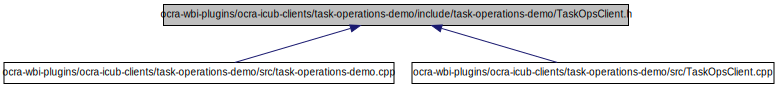
\includegraphics[width=350pt]{TaskOpsClient_8h__dep__incl}
\end{center}
\end{figure}
\subsection*{\-Classes}
\begin{DoxyCompactItemize}
\item 
class \hyperlink{classTaskOpsClient}{\-Task\-Ops\-Client}
\end{DoxyCompactItemize}
\subsection*{\-Enumerations}
\begin{DoxyCompactItemize}
\item 
enum \hyperlink{TaskOpsClient_8h_a0140057ae3fbe1db5f5c418dfc67d9db}{\-T\-H\-I\-N\-G\-S\-\_\-\-T\-O\-\_\-\-D\-O} \{ \*
\hyperlink{TaskOpsClient_8h_a0140057ae3fbe1db5f5c418dfc67d9dbaf831abed77e2c76cacc256b8b16f2b2a}{\-R\-E\-M\-O\-V\-E\-\_\-\-T\-A\-S\-K}, 
\hyperlink{TaskOpsClient_8h_a0140057ae3fbe1db5f5c418dfc67d9dba6aa666a68fed72da5438e0ef9b7cba8f}{\-A\-D\-D\-\_\-\-N\-E\-W\-\_\-\-T\-A\-S\-K}, 
\hyperlink{TaskOpsClient_8h_a0140057ae3fbe1db5f5c418dfc67d9dba8ffc9eba853106ab798ee2a0c5763d1b}{\-A\-D\-D\-\_\-\-E\-X\-I\-S\-T\-I\-N\-G\-\_\-\-T\-A\-S\-K}, 
\hyperlink{TaskOpsClient_8h_a0140057ae3fbe1db5f5c418dfc67d9dba7eaf30861bc723f003ea1a8e4a7a4977}{\-A\-D\-D\-\_\-\-E\-X\-I\-S\-T\-I\-N\-G\-\_\-\-T\-A\-S\-K\-\_\-\-N\-O\-\_\-\-O\-V\-E\-R\-W\-R\-I\-T\-E}, 
\*
\hyperlink{TaskOpsClient_8h_a0140057ae3fbe1db5f5c418dfc67d9dbacfe24a7b308a82835c8a9a9a89bc4ca2}{\-N\-O\-T\-H\-I\-N\-G}
 \}
\end{DoxyCompactItemize}


\subsection{\-Enumeration \-Type \-Documentation}
\hypertarget{TaskOpsClient_8h_a0140057ae3fbe1db5f5c418dfc67d9db}{\index{\-Task\-Ops\-Client.\-h@{\-Task\-Ops\-Client.\-h}!\-T\-H\-I\-N\-G\-S\-\_\-\-T\-O\-\_\-\-D\-O@{\-T\-H\-I\-N\-G\-S\-\_\-\-T\-O\-\_\-\-D\-O}}
\index{\-T\-H\-I\-N\-G\-S\-\_\-\-T\-O\-\_\-\-D\-O@{\-T\-H\-I\-N\-G\-S\-\_\-\-T\-O\-\_\-\-D\-O}!TaskOpsClient.h@{\-Task\-Ops\-Client.\-h}}
\subsubsection[{\-T\-H\-I\-N\-G\-S\-\_\-\-T\-O\-\_\-\-D\-O}]{\setlength{\rightskip}{0pt plus 5cm}enum {\bf \-T\-H\-I\-N\-G\-S\-\_\-\-T\-O\-\_\-\-D\-O}}}\label{TaskOpsClient_8h_a0140057ae3fbe1db5f5c418dfc67d9db}
\begin{Desc}
\item[\-Enumerator\-: ]\par
\begin{description}
\index{\-R\-E\-M\-O\-V\-E\-\_\-\-T\-A\-S\-K@{\-R\-E\-M\-O\-V\-E\-\_\-\-T\-A\-S\-K}!\-Task\-Ops\-Client.\-h@{\-Task\-Ops\-Client.\-h}}\index{\-Task\-Ops\-Client.\-h@{\-Task\-Ops\-Client.\-h}!\-R\-E\-M\-O\-V\-E\-\_\-\-T\-A\-S\-K@{\-R\-E\-M\-O\-V\-E\-\_\-\-T\-A\-S\-K}}\item[{\em 
\hypertarget{TaskOpsClient_8h_a0140057ae3fbe1db5f5c418dfc67d9dbaf831abed77e2c76cacc256b8b16f2b2a}{\-R\-E\-M\-O\-V\-E\-\_\-\-T\-A\-S\-K}\label{TaskOpsClient_8h_a0140057ae3fbe1db5f5c418dfc67d9dbaf831abed77e2c76cacc256b8b16f2b2a}
}]\index{\-A\-D\-D\-\_\-\-N\-E\-W\-\_\-\-T\-A\-S\-K@{\-A\-D\-D\-\_\-\-N\-E\-W\-\_\-\-T\-A\-S\-K}!\-Task\-Ops\-Client.\-h@{\-Task\-Ops\-Client.\-h}}\index{\-Task\-Ops\-Client.\-h@{\-Task\-Ops\-Client.\-h}!\-A\-D\-D\-\_\-\-N\-E\-W\-\_\-\-T\-A\-S\-K@{\-A\-D\-D\-\_\-\-N\-E\-W\-\_\-\-T\-A\-S\-K}}\item[{\em 
\hypertarget{TaskOpsClient_8h_a0140057ae3fbe1db5f5c418dfc67d9dba6aa666a68fed72da5438e0ef9b7cba8f}{\-A\-D\-D\-\_\-\-N\-E\-W\-\_\-\-T\-A\-S\-K}\label{TaskOpsClient_8h_a0140057ae3fbe1db5f5c418dfc67d9dba6aa666a68fed72da5438e0ef9b7cba8f}
}]\index{\-A\-D\-D\-\_\-\-E\-X\-I\-S\-T\-I\-N\-G\-\_\-\-T\-A\-S\-K@{\-A\-D\-D\-\_\-\-E\-X\-I\-S\-T\-I\-N\-G\-\_\-\-T\-A\-S\-K}!\-Task\-Ops\-Client.\-h@{\-Task\-Ops\-Client.\-h}}\index{\-Task\-Ops\-Client.\-h@{\-Task\-Ops\-Client.\-h}!\-A\-D\-D\-\_\-\-E\-X\-I\-S\-T\-I\-N\-G\-\_\-\-T\-A\-S\-K@{\-A\-D\-D\-\_\-\-E\-X\-I\-S\-T\-I\-N\-G\-\_\-\-T\-A\-S\-K}}\item[{\em 
\hypertarget{TaskOpsClient_8h_a0140057ae3fbe1db5f5c418dfc67d9dba8ffc9eba853106ab798ee2a0c5763d1b}{\-A\-D\-D\-\_\-\-E\-X\-I\-S\-T\-I\-N\-G\-\_\-\-T\-A\-S\-K}\label{TaskOpsClient_8h_a0140057ae3fbe1db5f5c418dfc67d9dba8ffc9eba853106ab798ee2a0c5763d1b}
}]\index{\-A\-D\-D\-\_\-\-E\-X\-I\-S\-T\-I\-N\-G\-\_\-\-T\-A\-S\-K\-\_\-\-N\-O\-\_\-\-O\-V\-E\-R\-W\-R\-I\-T\-E@{\-A\-D\-D\-\_\-\-E\-X\-I\-S\-T\-I\-N\-G\-\_\-\-T\-A\-S\-K\-\_\-\-N\-O\-\_\-\-O\-V\-E\-R\-W\-R\-I\-T\-E}!\-Task\-Ops\-Client.\-h@{\-Task\-Ops\-Client.\-h}}\index{\-Task\-Ops\-Client.\-h@{\-Task\-Ops\-Client.\-h}!\-A\-D\-D\-\_\-\-E\-X\-I\-S\-T\-I\-N\-G\-\_\-\-T\-A\-S\-K\-\_\-\-N\-O\-\_\-\-O\-V\-E\-R\-W\-R\-I\-T\-E@{\-A\-D\-D\-\_\-\-E\-X\-I\-S\-T\-I\-N\-G\-\_\-\-T\-A\-S\-K\-\_\-\-N\-O\-\_\-\-O\-V\-E\-R\-W\-R\-I\-T\-E}}\item[{\em 
\hypertarget{TaskOpsClient_8h_a0140057ae3fbe1db5f5c418dfc67d9dba7eaf30861bc723f003ea1a8e4a7a4977}{\-A\-D\-D\-\_\-\-E\-X\-I\-S\-T\-I\-N\-G\-\_\-\-T\-A\-S\-K\-\_\-\-N\-O\-\_\-\-O\-V\-E\-R\-W\-R\-I\-T\-E}\label{TaskOpsClient_8h_a0140057ae3fbe1db5f5c418dfc67d9dba7eaf30861bc723f003ea1a8e4a7a4977}
}]\index{\-N\-O\-T\-H\-I\-N\-G@{\-N\-O\-T\-H\-I\-N\-G}!\-Task\-Ops\-Client.\-h@{\-Task\-Ops\-Client.\-h}}\index{\-Task\-Ops\-Client.\-h@{\-Task\-Ops\-Client.\-h}!\-N\-O\-T\-H\-I\-N\-G@{\-N\-O\-T\-H\-I\-N\-G}}\item[{\em 
\hypertarget{TaskOpsClient_8h_a0140057ae3fbe1db5f5c418dfc67d9dbacfe24a7b308a82835c8a9a9a89bc4ca2}{\-N\-O\-T\-H\-I\-N\-G}\label{TaskOpsClient_8h_a0140057ae3fbe1db5f5c418dfc67d9dbacfe24a7b308a82835c8a9a9a89bc4ca2}
}]\end{description}
\end{Desc}


\hypertarget{task-operations-demo_8cpp}{\section{ocra-\/wbi-\/plugins/ocra-\/icub-\/clients/task-\/operations-\/demo/src/task-\/operations-\/demo.cpp \-File \-Reference}
\label{task-operations-demo_8cpp}\index{ocra-\/wbi-\/plugins/ocra-\/icub-\/clients/task-\/operations-\/demo/src/task-\/operations-\/demo.\-cpp@{ocra-\/wbi-\/plugins/ocra-\/icub-\/clients/task-\/operations-\/demo/src/task-\/operations-\/demo.\-cpp}}
}
{\ttfamily \#include $<$yarp/os/\-Resource\-Finder.\-h$>$}\*
{\ttfamily \#include $<$yarp/os/\-Network.\-h$>$}\*
{\ttfamily \#include $<$yarp/os/\-Log.\-h$>$}\*
{\ttfamily \#include $<$yarp/os/\-Log\-Stream.\-h$>$}\*
{\ttfamily \#include $<$yarp/os/\-Time.\-h$>$}\*
{\ttfamily \#include \char`\"{}task-\/operations-\/demo/\-Task\-Ops\-Client.\-h\char`\"{}}\*
{\ttfamily \#include $<$ocra-\/icub/\-Icub\-Client.\-h$>$}\*
{\ttfamily \#include $<$ocra-\/recipes/\-Controller\-Client.\-h$>$}\*
{\ttfamily \#include $<$ocra-\/recipes/\-Client\-Manager.\-h$>$}\*
\-Include dependency graph for task-\/operations-\/demo.cpp\-:\nopagebreak
\begin{figure}[H]
\begin{center}
\leavevmode
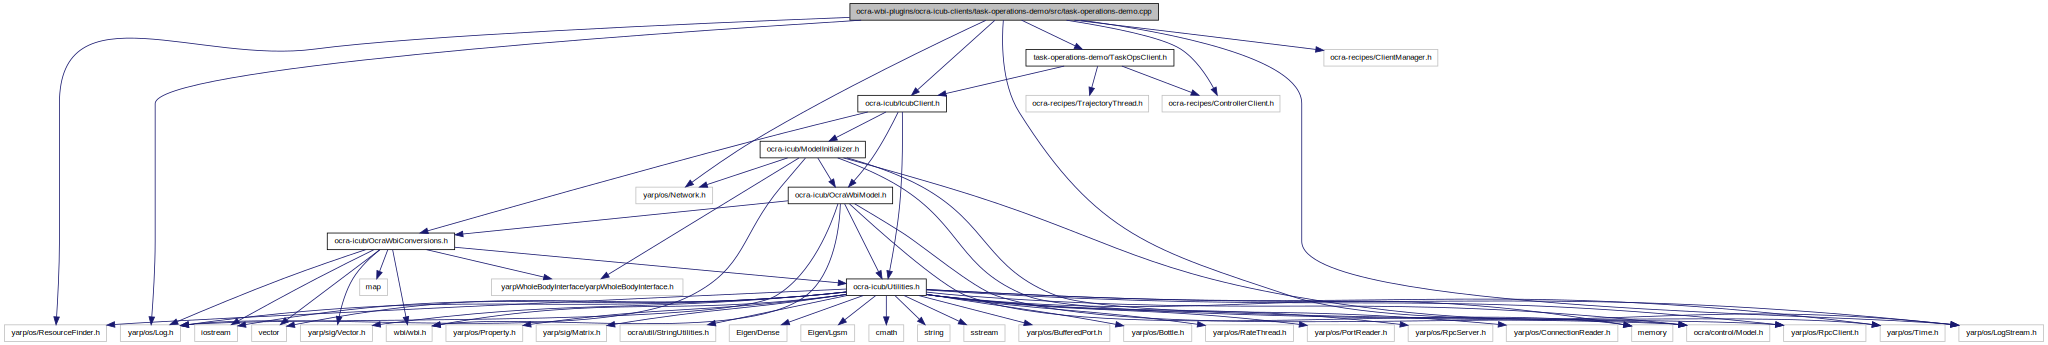
\includegraphics[width=350pt]{task-operations-demo_8cpp__incl}
\end{center}
\end{figure}
\subsection*{\-Functions}
\begin{DoxyCompactItemize}
\item 
int \hyperlink{task-operations-demo_8cpp_a0ddf1224851353fc92bfbff6f499fa97}{main} (int argc, char $\ast$argv\mbox{[}$\,$\mbox{]})
\end{DoxyCompactItemize}


\subsection{\-Function \-Documentation}
\hypertarget{task-operations-demo_8cpp_a0ddf1224851353fc92bfbff6f499fa97}{\index{task-\/operations-\/demo.\-cpp@{task-\/operations-\/demo.\-cpp}!main@{main}}
\index{main@{main}!task-operations-demo.cpp@{task-\/operations-\/demo.\-cpp}}
\subsubsection[{main}]{\setlength{\rightskip}{0pt plus 5cm}int {\bf main} (
\begin{DoxyParamCaption}
\item[{int}]{argc, }
\item[{char $\ast$}]{argv\mbox{[}$\,$\mbox{]}}
\end{DoxyParamCaption}
)}}\label{task-operations-demo_8cpp_a0ddf1224851353fc92bfbff6f499fa97}

\hypertarget{TaskOpsClient_8cpp}{\section{ocra-\/wbi-\/plugins/ocra-\/icub-\/clients/task-\/operations-\/demo/src/\-Task\-Ops\-Client.cpp \-File \-Reference}
\label{TaskOpsClient_8cpp}\index{ocra-\/wbi-\/plugins/ocra-\/icub-\/clients/task-\/operations-\/demo/src/\-Task\-Ops\-Client.\-cpp@{ocra-\/wbi-\/plugins/ocra-\/icub-\/clients/task-\/operations-\/demo/src/\-Task\-Ops\-Client.\-cpp}}
}
{\ttfamily \#include \char`\"{}task-\/operations-\/demo/\-Task\-Ops\-Client.\-h\char`\"{}}\*
\-Include dependency graph for \-Task\-Ops\-Client.\-cpp\-:
\nopagebreak
\begin{figure}[H]
\begin{center}
\leavevmode
\includegraphics[width=350pt]{TaskOpsClient_8cpp__incl}
\end{center}
\end{figure}

\hypertarget{WalkingClient_8h}{\section{ocra-\/wbi-\/plugins/ocra-\/icub-\/clients/walking-\/client/include/walking-\/client/\-Walking\-Client.h \-File \-Reference}
\label{WalkingClient_8h}\index{ocra-\/wbi-\/plugins/ocra-\/icub-\/clients/walking-\/client/include/walking-\/client/\-Walking\-Client.\-h@{ocra-\/wbi-\/plugins/ocra-\/icub-\/clients/walking-\/client/include/walking-\/client/\-Walking\-Client.\-h}}
}
{\ttfamily \#include $<$ocra-\/icub/\-Icub\-Client.\-h$>$}\*
{\ttfamily \#include $<$ocra-\/recipes/\-Trajectory\-Thread.\-h$>$}\*
{\ttfamily \#include $<$ocra-\/recipes/\-Controller\-Client.\-h$>$}\*
{\ttfamily \#include $<$ocra/util/\-Eigen\-Utilities.\-h$>$}\*
{\ttfamily \#include \char`\"{}walking-\/client/\-Zmp\-Preview\-Controller.\-h\char`\"{}}\*
{\ttfamily \#include $<$ocra/util/\-File\-Operations.\-h$>$}\*
{\ttfamily \#include $<$yarp/os/\-Time.\-h$>$}\*
\-Include dependency graph for \-Walking\-Client.\-h\-:\nopagebreak
\begin{figure}[H]
\begin{center}
\leavevmode
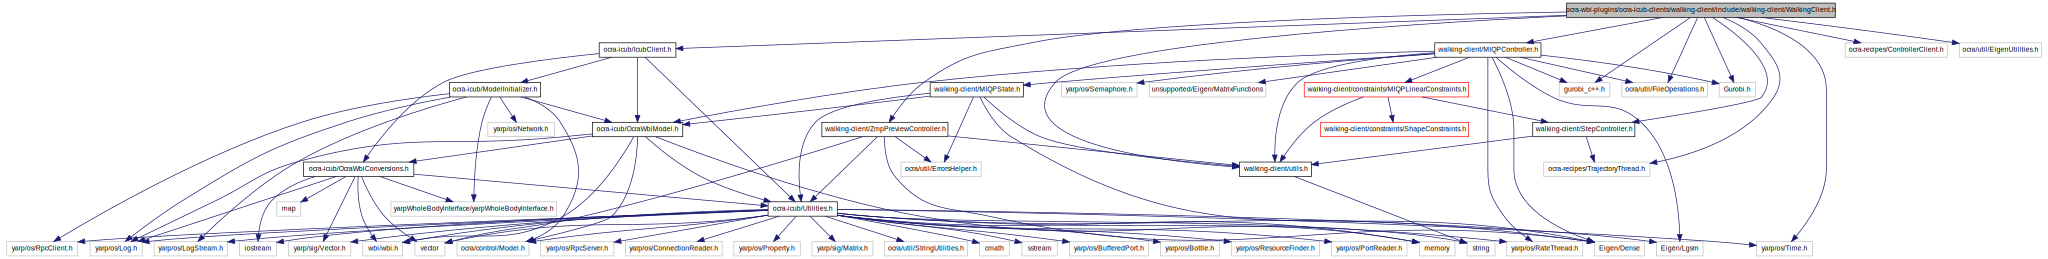
\includegraphics[width=350pt]{WalkingClient_8h__incl}
\end{center}
\end{figure}
\-This graph shows which files directly or indirectly include this file\-:\nopagebreak
\begin{figure}[H]
\begin{center}
\leavevmode
\includegraphics[width=350pt]{WalkingClient_8h__dep__incl}
\end{center}
\end{figure}
\subsection*{\-Classes}
\begin{DoxyCompactItemize}
\item 
class \hyperlink{classWalkingClient}{\-Walking\-Client}
\end{DoxyCompactItemize}
\subsection*{\-Enumerations}
\begin{DoxyCompactItemize}
\item 
enum \hyperlink{WalkingClient_8h_afc01479a47f5a87462a54b6a9e11fffa}{\-Zmp\-Test\-Type} \{ \hyperlink{WalkingClient_8h_afc01479a47f5a87462a54b6a9e11fffaa648ff770c850b8352c3306c1659e8157}{\-Z\-M\-P\-\_\-\-C\-O\-N\-S\-T\-A\-N\-T\-\_\-\-R\-E\-F\-E\-R\-E\-N\-C\-E} = 0, 
\hyperlink{WalkingClient_8h_afc01479a47f5a87462a54b6a9e11fffaa97cb99b5fec95c1f2945d3b33455b139}{\-Z\-M\-P\-\_\-\-V\-A\-R\-Y\-I\-N\-G\-\_\-\-R\-E\-F\-E\-R\-E\-N\-C\-E}, 
\hyperlink{WalkingClient_8h_afc01479a47f5a87462a54b6a9e11fffaad20e2ca429f4e3ba50e1de174c92af60}{\-C\-O\-M\-\_\-\-L\-I\-N\-\_\-\-V\-E\-L\-\_\-\-C\-O\-N\-S\-T\-A\-N\-T\-\_\-\-R\-E\-F\-E\-R\-E\-N\-C\-E}
 \}
\end{DoxyCompactItemize}


\subsection{\-Enumeration \-Type \-Documentation}
\hypertarget{WalkingClient_8h_afc01479a47f5a87462a54b6a9e11fffa}{\index{\-Walking\-Client.\-h@{\-Walking\-Client.\-h}!\-Zmp\-Test\-Type@{\-Zmp\-Test\-Type}}
\index{\-Zmp\-Test\-Type@{\-Zmp\-Test\-Type}!WalkingClient.h@{\-Walking\-Client.\-h}}
\subsubsection[{\-Zmp\-Test\-Type}]{\setlength{\rightskip}{0pt plus 5cm}enum {\bf \-Zmp\-Test\-Type}}}\label{WalkingClient_8h_afc01479a47f5a87462a54b6a9e11fffa}
\-Performs tests helpful to tune the gains used by the zmp and zmp preview controllers as well as the \-C\-O\-M task. \-See configure() for additional information. \begin{Desc}
\item[\-Enumerator\-: ]\par
\begin{description}
\index{\-Z\-M\-P\-\_\-\-C\-O\-N\-S\-T\-A\-N\-T\-\_\-\-R\-E\-F\-E\-R\-E\-N\-C\-E@{\-Z\-M\-P\-\_\-\-C\-O\-N\-S\-T\-A\-N\-T\-\_\-\-R\-E\-F\-E\-R\-E\-N\-C\-E}!\-Walking\-Client.\-h@{\-Walking\-Client.\-h}}\index{\-Walking\-Client.\-h@{\-Walking\-Client.\-h}!\-Z\-M\-P\-\_\-\-C\-O\-N\-S\-T\-A\-N\-T\-\_\-\-R\-E\-F\-E\-R\-E\-N\-C\-E@{\-Z\-M\-P\-\_\-\-C\-O\-N\-S\-T\-A\-N\-T\-\_\-\-R\-E\-F\-E\-R\-E\-N\-C\-E}}\item[{\em 
\hypertarget{WalkingClient_8h_afc01479a47f5a87462a54b6a9e11fffaa648ff770c850b8352c3306c1659e8157}{\-Z\-M\-P\-\_\-\-C\-O\-N\-S\-T\-A\-N\-T\-\_\-\-R\-E\-F\-E\-R\-E\-N\-C\-E}\label{WalkingClient_8h_afc01479a47f5a87462a54b6a9e11fffaa648ff770c850b8352c3306c1659e8157}
}]\index{\-Z\-M\-P\-\_\-\-V\-A\-R\-Y\-I\-N\-G\-\_\-\-R\-E\-F\-E\-R\-E\-N\-C\-E@{\-Z\-M\-P\-\_\-\-V\-A\-R\-Y\-I\-N\-G\-\_\-\-R\-E\-F\-E\-R\-E\-N\-C\-E}!\-Walking\-Client.\-h@{\-Walking\-Client.\-h}}\index{\-Walking\-Client.\-h@{\-Walking\-Client.\-h}!\-Z\-M\-P\-\_\-\-V\-A\-R\-Y\-I\-N\-G\-\_\-\-R\-E\-F\-E\-R\-E\-N\-C\-E@{\-Z\-M\-P\-\_\-\-V\-A\-R\-Y\-I\-N\-G\-\_\-\-R\-E\-F\-E\-R\-E\-N\-C\-E}}\item[{\em 
\hypertarget{WalkingClient_8h_afc01479a47f5a87462a54b6a9e11fffaa97cb99b5fec95c1f2945d3b33455b139}{\-Z\-M\-P\-\_\-\-V\-A\-R\-Y\-I\-N\-G\-\_\-\-R\-E\-F\-E\-R\-E\-N\-C\-E}\label{WalkingClient_8h_afc01479a47f5a87462a54b6a9e11fffaa97cb99b5fec95c1f2945d3b33455b139}
}]\index{\-C\-O\-M\-\_\-\-L\-I\-N\-\_\-\-V\-E\-L\-\_\-\-C\-O\-N\-S\-T\-A\-N\-T\-\_\-\-R\-E\-F\-E\-R\-E\-N\-C\-E@{\-C\-O\-M\-\_\-\-L\-I\-N\-\_\-\-V\-E\-L\-\_\-\-C\-O\-N\-S\-T\-A\-N\-T\-\_\-\-R\-E\-F\-E\-R\-E\-N\-C\-E}!\-Walking\-Client.\-h@{\-Walking\-Client.\-h}}\index{\-Walking\-Client.\-h@{\-Walking\-Client.\-h}!\-C\-O\-M\-\_\-\-L\-I\-N\-\_\-\-V\-E\-L\-\_\-\-C\-O\-N\-S\-T\-A\-N\-T\-\_\-\-R\-E\-F\-E\-R\-E\-N\-C\-E@{\-C\-O\-M\-\_\-\-L\-I\-N\-\_\-\-V\-E\-L\-\_\-\-C\-O\-N\-S\-T\-A\-N\-T\-\_\-\-R\-E\-F\-E\-R\-E\-N\-C\-E}}\item[{\em 
\hypertarget{WalkingClient_8h_afc01479a47f5a87462a54b6a9e11fffaad20e2ca429f4e3ba50e1de174c92af60}{\-C\-O\-M\-\_\-\-L\-I\-N\-\_\-\-V\-E\-L\-\_\-\-C\-O\-N\-S\-T\-A\-N\-T\-\_\-\-R\-E\-F\-E\-R\-E\-N\-C\-E}\label{WalkingClient_8h_afc01479a47f5a87462a54b6a9e11fffaad20e2ca429f4e3ba50e1de174c92af60}
}]\end{description}
\end{Desc}


\hypertarget{ZmpController_8h}{\section{ocra-\/wbi-\/plugins/ocra-\/icub-\/clients/walking-\/client/include/walking-\/client/\-Zmp\-Controller.h \-File \-Reference}
\label{ZmpController_8h}\index{ocra-\/wbi-\/plugins/ocra-\/icub-\/clients/walking-\/client/include/walking-\/client/\-Zmp\-Controller.\-h@{ocra-\/wbi-\/plugins/ocra-\/icub-\/clients/walking-\/client/include/walking-\/client/\-Zmp\-Controller.\-h}}
}
{\ttfamily \#include $<$ocra-\/icub/\-Utilities.\-h$>$}\*
{\ttfamily \#include $<$ocra/util/\-Errors\-Helper.\-h$>$}\*
{\ttfamily \#include $<$ocra/util/\-Eigen\-Utilities.\-h$>$}\*
{\ttfamily \#include $<$ocra/control/\-Task\-State.\-h$>$}\*
{\ttfamily \#include $<$ocra-\/recipes/\-Task\-Connection.\-h$>$}\*
{\ttfamily \#include $<$\-Eigen/\-Dense$>$}\*
{\ttfamily \#include $<$vector$>$}\*
\-Include dependency graph for \-Zmp\-Controller.\-h\-:
\nopagebreak
\begin{figure}[H]
\begin{center}
\leavevmode
\includegraphics[width=350pt]{ZmpController_8h__incl}
\end{center}
\end{figure}
\-This graph shows which files directly or indirectly include this file\-:\nopagebreak
\begin{figure}[H]
\begin{center}
\leavevmode
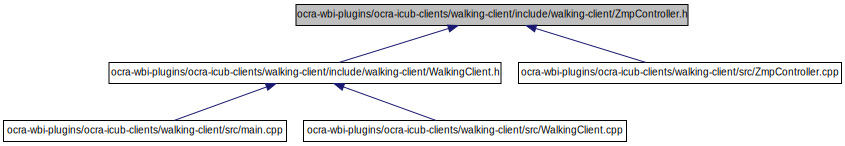
\includegraphics[width=350pt]{ZmpController_8h__dep__incl}
\end{center}
\end{figure}
\subsection*{\-Classes}
\begin{DoxyCompactItemize}
\item 
struct \hyperlink{structZmpControllerParams}{\-Zmp\-Controller\-Params}
\item 
class \hyperlink{classZmpController}{\-Zmp\-Controller}
\begin{DoxyCompactList}\small\item\em \-Implementes a \-Z\-M\-P controller as a force set point regulator. \end{DoxyCompactList}\end{DoxyCompactItemize}
\subsection*{\-Enumerations}
\begin{DoxyCompactItemize}
\item 
enum \hyperlink{ZmpController_8h_a4b6a8e135f90bd56e5a57a60efb42529}{\-F\-O\-O\-T} \{ \hyperlink{ZmpController_8h_a4b6a8e135f90bd56e5a57a60efb42529a7760daad9db1ede8c57b06189deca9f3}{\-L\-E\-F\-T\-\_\-\-F\-O\-O\-T}, 
\hyperlink{ZmpController_8h_a4b6a8e135f90bd56e5a57a60efb42529ace119c66af60ac0781b137aa87d7be62}{\-R\-I\-G\-H\-T\-\_\-\-F\-O\-O\-T}
 \}
\end{DoxyCompactItemize}


\subsection{\-Enumeration \-Type \-Documentation}
\hypertarget{ZmpController_8h_a4b6a8e135f90bd56e5a57a60efb42529}{\index{\-Zmp\-Controller.\-h@{\-Zmp\-Controller.\-h}!\-F\-O\-O\-T@{\-F\-O\-O\-T}}
\index{\-F\-O\-O\-T@{\-F\-O\-O\-T}!ZmpController.h@{\-Zmp\-Controller.\-h}}
\subsubsection[{\-F\-O\-O\-T}]{\setlength{\rightskip}{0pt plus 5cm}enum {\bf \-F\-O\-O\-T}}}\label{ZmpController_8h_a4b6a8e135f90bd56e5a57a60efb42529}
\begin{Desc}
\item[\-Enumerator\-: ]\par
\begin{description}
\index{\-L\-E\-F\-T\-\_\-\-F\-O\-O\-T@{\-L\-E\-F\-T\-\_\-\-F\-O\-O\-T}!\-Zmp\-Controller.\-h@{\-Zmp\-Controller.\-h}}\index{\-Zmp\-Controller.\-h@{\-Zmp\-Controller.\-h}!\-L\-E\-F\-T\-\_\-\-F\-O\-O\-T@{\-L\-E\-F\-T\-\_\-\-F\-O\-O\-T}}\item[{\em 
\hypertarget{ZmpController_8h_a4b6a8e135f90bd56e5a57a60efb42529a7760daad9db1ede8c57b06189deca9f3}{\-L\-E\-F\-T\-\_\-\-F\-O\-O\-T}\label{ZmpController_8h_a4b6a8e135f90bd56e5a57a60efb42529a7760daad9db1ede8c57b06189deca9f3}
}]\index{\-R\-I\-G\-H\-T\-\_\-\-F\-O\-O\-T@{\-R\-I\-G\-H\-T\-\_\-\-F\-O\-O\-T}!\-Zmp\-Controller.\-h@{\-Zmp\-Controller.\-h}}\index{\-Zmp\-Controller.\-h@{\-Zmp\-Controller.\-h}!\-R\-I\-G\-H\-T\-\_\-\-F\-O\-O\-T@{\-R\-I\-G\-H\-T\-\_\-\-F\-O\-O\-T}}\item[{\em 
\hypertarget{ZmpController_8h_a4b6a8e135f90bd56e5a57a60efb42529ace119c66af60ac0781b137aa87d7be62}{\-R\-I\-G\-H\-T\-\_\-\-F\-O\-O\-T}\label{ZmpController_8h_a4b6a8e135f90bd56e5a57a60efb42529ace119c66af60ac0781b137aa87d7be62}
}]\end{description}
\end{Desc}


\hypertarget{ZmpPreviewController_8h}{\section{ocra-\/wbi-\/plugins/ocra-\/icub-\/clients/walking-\/client/include/walking-\/client/\-Zmp\-Preview\-Controller.h \-File \-Reference}
\label{ZmpPreviewController_8h}\index{ocra-\/wbi-\/plugins/ocra-\/icub-\/clients/walking-\/client/include/walking-\/client/\-Zmp\-Preview\-Controller.\-h@{ocra-\/wbi-\/plugins/ocra-\/icub-\/clients/walking-\/client/include/walking-\/client/\-Zmp\-Preview\-Controller.\-h}}
}
{\ttfamily \#include $<$ocra-\/icub/\-Utilities.\-h$>$}\*
{\ttfamily \#include $<$ocra/util/\-Errors\-Helper.\-h$>$}\*
{\ttfamily \#include $<$\-Eigen/\-Dense$>$}\*
{\ttfamily \#include $<$vector$>$}\*
\-Include dependency graph for \-Zmp\-Preview\-Controller.\-h\-:
\nopagebreak
\begin{figure}[H]
\begin{center}
\leavevmode
\includegraphics[width=350pt]{ZmpPreviewController_8h__incl}
\end{center}
\end{figure}
\-This graph shows which files directly or indirectly include this file\-:\nopagebreak
\begin{figure}[H]
\begin{center}
\leavevmode
\includegraphics[width=350pt]{ZmpPreviewController_8h__dep__incl}
\end{center}
\end{figure}
\subsection*{\-Classes}
\begin{DoxyCompactItemize}
\item 
struct \hyperlink{structZmpPreviewParams}{\-Zmp\-Preview\-Params}
\item 
class \hyperlink{classZmpPreviewController}{\-Zmp\-Preview\-Controller}
\begin{DoxyCompactList}\small\item\em \-Implementes an extended \-Z\-M\-P preview controller as an unconstrained \-Q\-P problem. \end{DoxyCompactList}\end{DoxyCompactItemize}
\subsection*{\-Enumerations}
\begin{DoxyCompactItemize}
\item 
enum \hyperlink{ZmpPreviewController_8h_a4b6a8e135f90bd56e5a57a60efb42529}{\-F\-O\-O\-T} \{ \hyperlink{ZmpController_8h_a4b6a8e135f90bd56e5a57a60efb42529a7760daad9db1ede8c57b06189deca9f3}{\-L\-E\-F\-T\-\_\-\-F\-O\-O\-T}, 
\hyperlink{ZmpController_8h_a4b6a8e135f90bd56e5a57a60efb42529ace119c66af60ac0781b137aa87d7be62}{\-R\-I\-G\-H\-T\-\_\-\-F\-O\-O\-T}, 
\hyperlink{ZmpPreviewController_8h_a4b6a8e135f90bd56e5a57a60efb42529a7760daad9db1ede8c57b06189deca9f3}{\-L\-E\-F\-T\-\_\-\-F\-O\-O\-T}, 
\hyperlink{ZmpPreviewController_8h_a4b6a8e135f90bd56e5a57a60efb42529ace119c66af60ac0781b137aa87d7be62}{\-R\-I\-G\-H\-T\-\_\-\-F\-O\-O\-T}
 \}
\end{DoxyCompactItemize}


\subsection{\-Enumeration \-Type \-Documentation}
\hypertarget{ZmpPreviewController_8h_a4b6a8e135f90bd56e5a57a60efb42529}{\index{\-Zmp\-Preview\-Controller.\-h@{\-Zmp\-Preview\-Controller.\-h}!\-F\-O\-O\-T@{\-F\-O\-O\-T}}
\index{\-F\-O\-O\-T@{\-F\-O\-O\-T}!ZmpPreviewController.h@{\-Zmp\-Preview\-Controller.\-h}}
\subsubsection[{\-F\-O\-O\-T}]{\setlength{\rightskip}{0pt plus 5cm}enum {\bf \-F\-O\-O\-T}}}\label{ZmpPreviewController_8h_a4b6a8e135f90bd56e5a57a60efb42529}
\begin{Desc}
\item[\-Enumerator\-: ]\par
\begin{description}
\index{\-L\-E\-F\-T\-\_\-\-F\-O\-O\-T@{\-L\-E\-F\-T\-\_\-\-F\-O\-O\-T}!\-Zmp\-Preview\-Controller.\-h@{\-Zmp\-Preview\-Controller.\-h}}\index{\-Zmp\-Preview\-Controller.\-h@{\-Zmp\-Preview\-Controller.\-h}!\-L\-E\-F\-T\-\_\-\-F\-O\-O\-T@{\-L\-E\-F\-T\-\_\-\-F\-O\-O\-T}}\item[{\em 
\hypertarget{ZmpPreviewController_8h_a4b6a8e135f90bd56e5a57a60efb42529a7760daad9db1ede8c57b06189deca9f3}{\-L\-E\-F\-T\-\_\-\-F\-O\-O\-T}\label{ZmpPreviewController_8h_a4b6a8e135f90bd56e5a57a60efb42529a7760daad9db1ede8c57b06189deca9f3}
}]\index{\-R\-I\-G\-H\-T\-\_\-\-F\-O\-O\-T@{\-R\-I\-G\-H\-T\-\_\-\-F\-O\-O\-T}!\-Zmp\-Preview\-Controller.\-h@{\-Zmp\-Preview\-Controller.\-h}}\index{\-Zmp\-Preview\-Controller.\-h@{\-Zmp\-Preview\-Controller.\-h}!\-R\-I\-G\-H\-T\-\_\-\-F\-O\-O\-T@{\-R\-I\-G\-H\-T\-\_\-\-F\-O\-O\-T}}\item[{\em 
\hypertarget{ZmpPreviewController_8h_a4b6a8e135f90bd56e5a57a60efb42529ace119c66af60ac0781b137aa87d7be62}{\-R\-I\-G\-H\-T\-\_\-\-F\-O\-O\-T}\label{ZmpPreviewController_8h_a4b6a8e135f90bd56e5a57a60efb42529ace119c66af60ac0781b137aa87d7be62}
}]\index{\-L\-E\-F\-T\-\_\-\-F\-O\-O\-T@{\-L\-E\-F\-T\-\_\-\-F\-O\-O\-T}!\-Zmp\-Preview\-Controller.\-h@{\-Zmp\-Preview\-Controller.\-h}}\index{\-Zmp\-Preview\-Controller.\-h@{\-Zmp\-Preview\-Controller.\-h}!\-L\-E\-F\-T\-\_\-\-F\-O\-O\-T@{\-L\-E\-F\-T\-\_\-\-F\-O\-O\-T}}\item[{\em 
\hypertarget{ZmpPreviewController_8h_a4b6a8e135f90bd56e5a57a60efb42529a7760daad9db1ede8c57b06189deca9f3}{\-L\-E\-F\-T\-\_\-\-F\-O\-O\-T}\label{ZmpPreviewController_8h_a4b6a8e135f90bd56e5a57a60efb42529a7760daad9db1ede8c57b06189deca9f3}
}]\index{\-R\-I\-G\-H\-T\-\_\-\-F\-O\-O\-T@{\-R\-I\-G\-H\-T\-\_\-\-F\-O\-O\-T}!\-Zmp\-Preview\-Controller.\-h@{\-Zmp\-Preview\-Controller.\-h}}\index{\-Zmp\-Preview\-Controller.\-h@{\-Zmp\-Preview\-Controller.\-h}!\-R\-I\-G\-H\-T\-\_\-\-F\-O\-O\-T@{\-R\-I\-G\-H\-T\-\_\-\-F\-O\-O\-T}}\item[{\em 
\hypertarget{ZmpPreviewController_8h_a4b6a8e135f90bd56e5a57a60efb42529ace119c66af60ac0781b137aa87d7be62}{\-R\-I\-G\-H\-T\-\_\-\-F\-O\-O\-T}\label{ZmpPreviewController_8h_a4b6a8e135f90bd56e5a57a60efb42529ace119c66af60ac0781b137aa87d7be62}
}]\end{description}
\end{Desc}


\hypertarget{WalkingClient_8cpp}{\section{ocra-\/wbi-\/plugins/ocra-\/icub-\/clients/walking-\/client/src/\-Walking\-Client.cpp \-File \-Reference}
\label{WalkingClient_8cpp}\index{ocra-\/wbi-\/plugins/ocra-\/icub-\/clients/walking-\/client/src/\-Walking\-Client.\-cpp@{ocra-\/wbi-\/plugins/ocra-\/icub-\/clients/walking-\/client/src/\-Walking\-Client.\-cpp}}
}
{\ttfamily \#include \char`\"{}walking-\/client/\-Walking\-Client.\-h\char`\"{}}\*
\-Include dependency graph for \-Walking\-Client.\-cpp\-:
\nopagebreak
\begin{figure}[H]
\begin{center}
\leavevmode
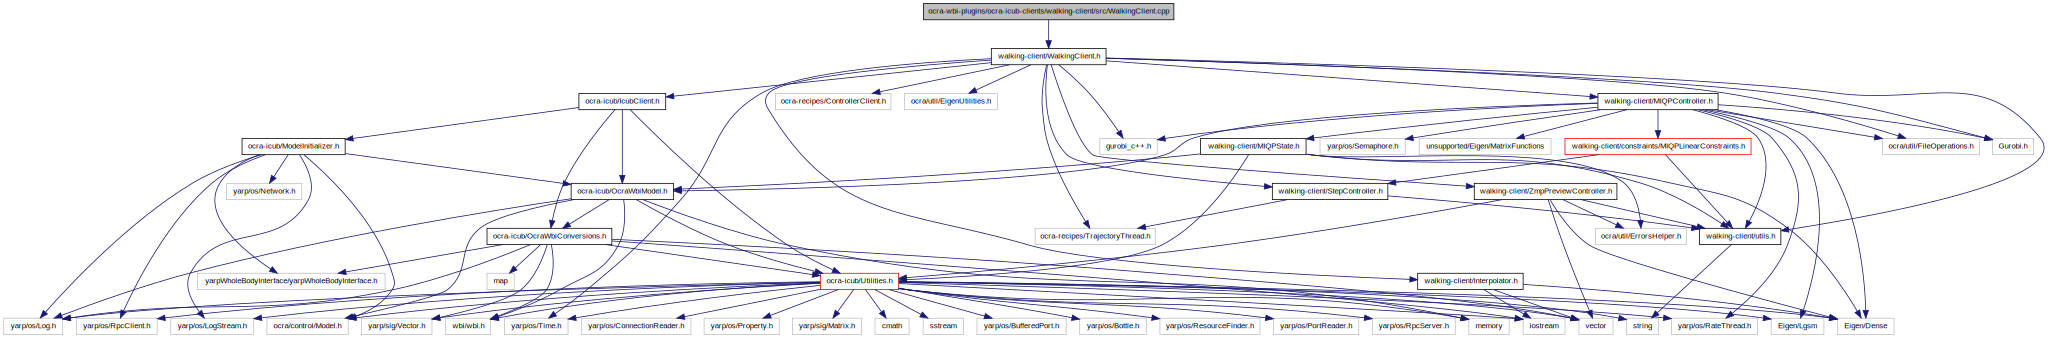
\includegraphics[width=350pt]{WalkingClient_8cpp__incl}
\end{center}
\end{figure}

\input{ZmpController_8cpp}
\input{ZmpPreviewController_8cpp}
\hypertarget{IcubControllerServer_8h}{\section{ocra-\/wbi-\/plugins/ocra-\/icub-\/server/include/ocra-\/icub-\/server/\-Icub\-Controller\-Server.h \-File \-Reference}
\label{IcubControllerServer_8h}\index{ocra-\/wbi-\/plugins/ocra-\/icub-\/server/include/ocra-\/icub-\/server/\-Icub\-Controller\-Server.\-h@{ocra-\/wbi-\/plugins/ocra-\/icub-\/server/include/ocra-\/icub-\/server/\-Icub\-Controller\-Server.\-h}}
}
{\ttfamily \#include $<$wbi/wbi.\-h$>$}\*
{\ttfamily \#include $<$ocra-\/recipes/\-Controller\-Server.\-h$>$}\*
{\ttfamily \#include $<$\-Eigen/\-Dense$>$}\*
{\ttfamily \#include $<$ocra-\/icub/\-Ocra\-Wbi\-Model.\-h$>$}\*
{\ttfamily \#include $<$i\-Dyn\-Tree/\-Estimation/\-Simple\-Legged\-Odometry.\-h$>$}\*
{\ttfamily \#include $<$ocra/util/\-Errors\-Helper.\-h$>$}\*
\-Include dependency graph for \-Icub\-Controller\-Server.\-h\-:\nopagebreak
\begin{figure}[H]
\begin{center}
\leavevmode
\includegraphics[width=350pt]{IcubControllerServer_8h__incl}
\end{center}
\end{figure}
\-This graph shows which files directly or indirectly include this file\-:\nopagebreak
\begin{figure}[H]
\begin{center}
\leavevmode
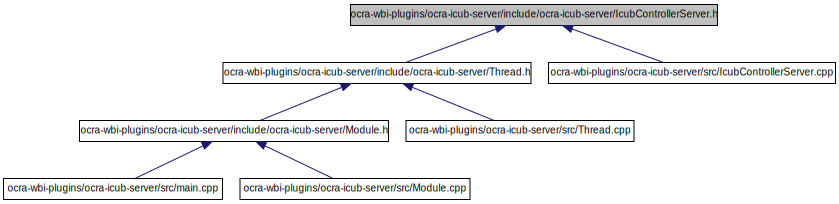
\includegraphics[width=350pt]{IcubControllerServer_8h__dep__incl}
\end{center}
\end{figure}
\subsection*{\-Classes}
\begin{DoxyCompactItemize}
\item 
class \hyperlink{classIcubControllerServer}{\-Icub\-Controller\-Server}
\end{DoxyCompactItemize}

\hypertarget{Module_8h}{\section{ocra-\/wbi-\/plugins/ocra-\/icub-\/server/include/ocra-\/icub-\/server/\-Module.h \-File \-Reference}
\label{Module_8h}\index{ocra-\/wbi-\/plugins/ocra-\/icub-\/server/include/ocra-\/icub-\/server/\-Module.\-h@{ocra-\/wbi-\/plugins/ocra-\/icub-\/server/include/ocra-\/icub-\/server/\-Module.\-h}}
}


\hyperlink{classModule}{\-Module} class for the controller server.  


{\ttfamily \#include $<$iostream$>$}\*
{\ttfamily \#include $<$memory$>$}\*
{\ttfamily \#include $<$algorithm$>$}\*
{\ttfamily \#include $<$locale$>$}\*
{\ttfamily \#include $<$yarp/os/\-R\-F\-Module.\-h$>$}\*
{\ttfamily \#include $<$yarp\-Whole\-Body\-Interface/yarp\-Whole\-Body\-Interface.\-h$>$}\*
{\ttfamily \#include \char`\"{}ocra-\/icub-\/server/\-Thread.\-h\char`\"{}}\*
{\ttfamily \#include \char`\"{}ocra-\/icub/\-Utilities.\-h\char`\"{}}\*
\-Include dependency graph for \-Module.\-h\-:
\nopagebreak
\begin{figure}[H]
\begin{center}
\leavevmode
\includegraphics[width=350pt]{Module_8h__incl}
\end{center}
\end{figure}
\-This graph shows which files directly or indirectly include this file\-:
\nopagebreak
\begin{figure}[H]
\begin{center}
\leavevmode
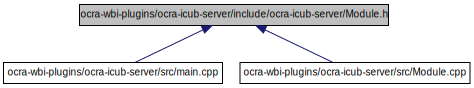
\includegraphics[width=350pt]{Module_8h__dep__incl}
\end{center}
\end{figure}
\subsection*{\-Classes}
\begin{DoxyCompactItemize}
\item 
class \hyperlink{classModule}{\-Module}
\begin{DoxyCompactList}\small\item\em \-The controller module which launches the controller thread. \end{DoxyCompactList}\end{DoxyCompactItemize}


\subsection{\-Detailed \-Description}
\hyperlink{classModule}{\-Module} class for the controller server. \begin{DoxyAuthor}{\-Author}
\mbox{[}\-Ryan \-Lober\mbox{]}(\href{http://www.ryanlober.com}{\tt http\-://www.\-ryanlober.\-com}) 

\mbox{[}\-Antoine \-Hoarau\mbox{]}(\href{http://ahoarau.github.io}{\tt http\-://ahoarau.\-github.\-io}) 
\end{DoxyAuthor}
\begin{DoxyDate}{\-Date}
\-Feb 2016 
\end{DoxyDate}
\begin{DoxyCopyright}{\-Copyright}
\-G\-N\-U \-General \-Public \-License. 
\end{DoxyCopyright}

\hypertarget{Thread_8h}{\section{ocra-\/wbi-\/plugins/ocra-\/icub-\/server/include/ocra-\/icub-\/server/\-Thread.h \-File \-Reference}
\label{Thread_8h}\index{ocra-\/wbi-\/plugins/ocra-\/icub-\/server/include/ocra-\/icub-\/server/\-Thread.\-h@{ocra-\/wbi-\/plugins/ocra-\/icub-\/server/include/ocra-\/icub-\/server/\-Thread.\-h}}
}


\-The thread class for the controller server.  


{\ttfamily \#include $<$yarp\-Whole\-Body\-Interface/yarp\-Whole\-Body\-Interface.\-h$>$}\*
{\ttfamily \#include $<$wbi/wbi.\-h$>$}\*
{\ttfamily \#include $<$ocra-\/icub-\/server/\-Icub\-Controller\-Server.\-h$>$}\*
{\ttfamily \#include $<$ocra-\/icub/\-Utilities.\-h$>$}\*
{\ttfamily \#include $<$ocra/util/\-Errors\-Helper.\-h$>$}\*
{\ttfamily \#include $<$yarp/os/\-Bottle.\-h$>$}\*
{\ttfamily \#include $<$yarp/os/\-Rpc\-Server.\-h$>$}\*
{\ttfamily \#include $<$yarp/os/\-Connection\-Reader.\-h$>$}\*
{\ttfamily \#include $<$yarp/os/\-Time.\-h$>$}\*
{\ttfamily \#include $<$sstream$>$}\*
{\ttfamily \#include $<$string$>$}\*
{\ttfamily \#include $<$i\-Dyn\-Tree/\-Estimation/\-Simple\-Legged\-Odometry.\-h$>$}\*
\-Include dependency graph for \-Thread.\-h\-:\nopagebreak
\begin{figure}[H]
\begin{center}
\leavevmode
\includegraphics[width=350pt]{Thread_8h__incl}
\end{center}
\end{figure}
\-This graph shows which files directly or indirectly include this file\-:\nopagebreak
\begin{figure}[H]
\begin{center}
\leavevmode
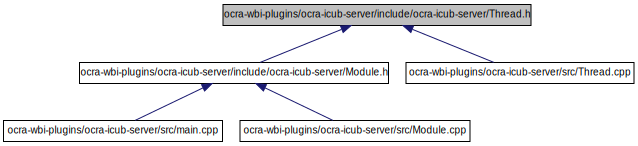
\includegraphics[width=350pt]{Thread_8h__dep__incl}
\end{center}
\end{figure}
\subsection*{\-Classes}
\begin{DoxyCompactItemize}
\item 
class \hyperlink{classOcraControllerOptions}{\-Ocra\-Controller\-Options}
\item 
class \hyperlink{classThread}{\-Thread}
\begin{DoxyCompactList}\small\item\em \-The meat and potatoes of the controller server. \end{DoxyCompactList}\item 
class \hyperlink{classThread_1_1ControllerRpcServerCallback}{\-Thread\-::\-Controller\-Rpc\-Server\-Callback}
\begin{DoxyCompactList}\small\item\em \-A callback function which binds the rpc server port opened in the contoller server module to the controller thread's parsing function. \end{DoxyCompactList}\item 
class \hyperlink{classThread_1_1DebugRpcServerCallback}{\-Thread\-::\-Debug\-Rpc\-Server\-Callback}
\begin{DoxyCompactList}\small\item\em \-A callback function which binds the rpc server port opened in the contoller server module to the controller thread's parsing function. \end{DoxyCompactList}\end{DoxyCompactItemize}


\subsection{\-Detailed \-Description}
\-The thread class for the controller server. \begin{DoxyAuthor}{\-Author}
\mbox{[}\-Ryan \-Lober\mbox{]}(\href{http://www.ryanlober.com}{\tt http\-://www.\-ryanlober.\-com}) 

\mbox{[}\-Antoine \-Hoarau\mbox{]}(\href{http://ahoarau.github.io}{\tt http\-://ahoarau.\-github.\-io}) 
\end{DoxyAuthor}
\begin{DoxyDate}{\-Date}
\-Feb 2016 
\end{DoxyDate}
\begin{DoxyCopyright}{\-Copyright}
\-G\-N\-U \-General \-Public \-License. 
\end{DoxyCopyright}

\hypertarget{IcubControllerServer_8cpp}{\section{ocra-\/wbi-\/plugins/ocra-\/icub-\/server/src/\-Icub\-Controller\-Server.cpp \-File \-Reference}
\label{IcubControllerServer_8cpp}\index{ocra-\/wbi-\/plugins/ocra-\/icub-\/server/src/\-Icub\-Controller\-Server.\-cpp@{ocra-\/wbi-\/plugins/ocra-\/icub-\/server/src/\-Icub\-Controller\-Server.\-cpp}}
}
{\ttfamily \#include $<$ocra-\/icub-\/server/\-Icub\-Controller\-Server.\-h$>$}\*
\-Include dependency graph for \-Icub\-Controller\-Server.\-cpp\-:\nopagebreak
\begin{figure}[H]
\begin{center}
\leavevmode
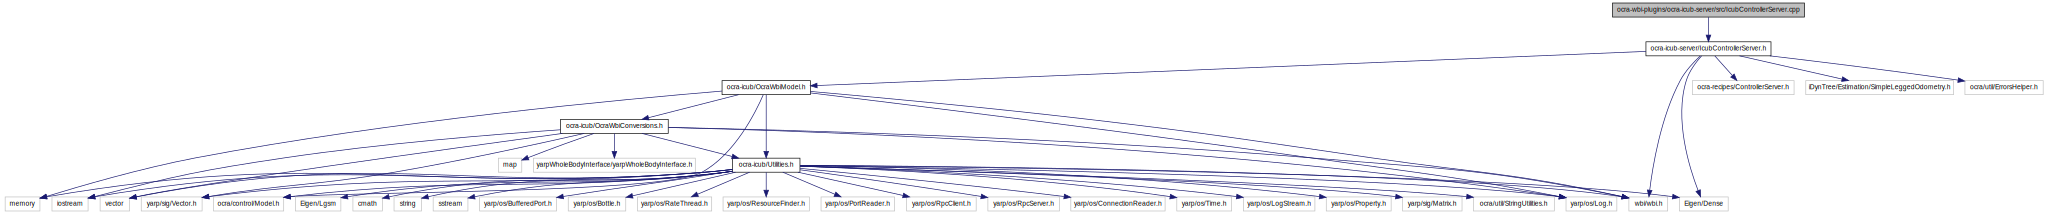
\includegraphics[width=350pt]{IcubControllerServer_8cpp__incl}
\end{center}
\end{figure}

\hypertarget{ocra-icub-server_2src_2main_8cpp}{\section{ocra-\/wbi-\/plugins/ocra-\/icub-\/server/src/main.cpp \-File \-Reference}
\label{ocra-icub-server_2src_2main_8cpp}\index{ocra-\/wbi-\/plugins/ocra-\/icub-\/server/src/main.\-cpp@{ocra-\/wbi-\/plugins/ocra-\/icub-\/server/src/main.\-cpp}}
}
{\ttfamily \#include $<$yarp/os/\-Resource\-Finder.\-h$>$}\*
{\ttfamily \#include $<$yarp/os/\-Network.\-h$>$}\*
{\ttfamily \#include $<$yarp/os/\-Log.\-h$>$}\*
{\ttfamily \#include $<$ocra-\/icub-\/server/\-Module.\-h$>$}\*
\-Include dependency graph for main.\-cpp\-:\nopagebreak
\begin{figure}[H]
\begin{center}
\leavevmode
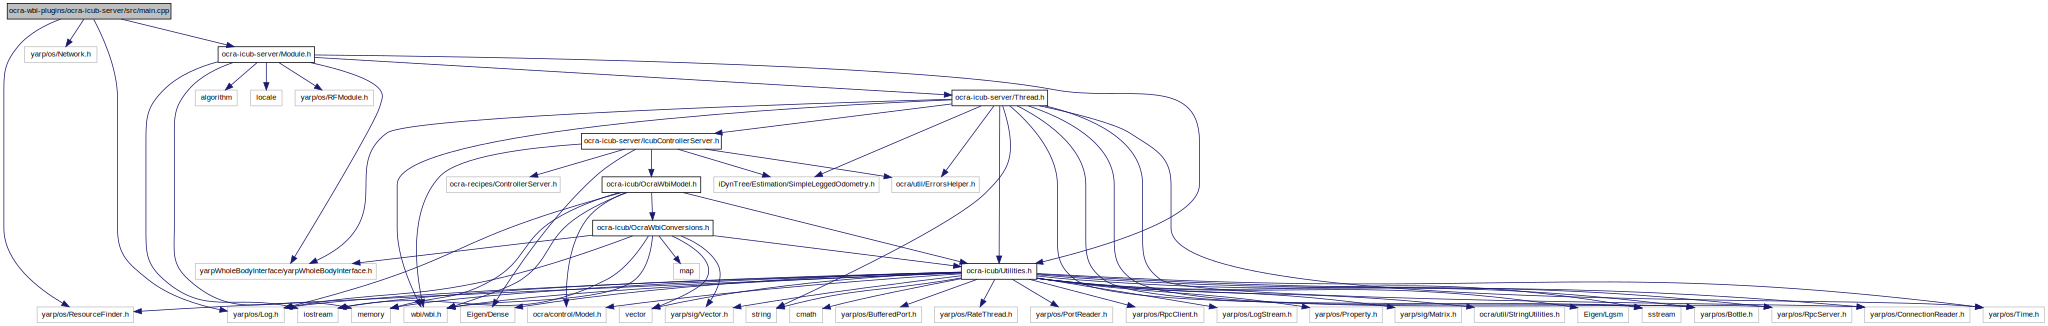
\includegraphics[width=350pt]{ocra-icub-server_2src_2main_8cpp__incl}
\end{center}
\end{figure}
\subsection*{\-Defines}
\begin{DoxyCompactItemize}
\item 
\#define \hyperlink{ocra-icub-server_2src_2main_8cpp_aacf7b13861a4ce37b8dec1979eb6450c}{\-D\-E\-F\-A\-U\-L\-T\-\_\-\-Y\-A\-R\-P\-\_\-\-C\-O\-N\-T\-E\-X\-T}~\char`\"{}ocra-\/icub-\/server\char`\"{}
\end{DoxyCompactItemize}
\subsection*{\-Functions}
\begin{DoxyCompactItemize}
\item 
int \hyperlink{ocra-icub-server_2src_2main_8cpp_a0ddf1224851353fc92bfbff6f499fa97}{main} (int argc, char $\ast$argv\mbox{[}$\,$\mbox{]})
\end{DoxyCompactItemize}


\subsection{\-Define \-Documentation}
\hypertarget{ocra-icub-server_2src_2main_8cpp_aacf7b13861a4ce37b8dec1979eb6450c}{\index{ocra-\/icub-\/server/src/main.\-cpp@{ocra-\/icub-\/server/src/main.\-cpp}!\-D\-E\-F\-A\-U\-L\-T\-\_\-\-Y\-A\-R\-P\-\_\-\-C\-O\-N\-T\-E\-X\-T@{\-D\-E\-F\-A\-U\-L\-T\-\_\-\-Y\-A\-R\-P\-\_\-\-C\-O\-N\-T\-E\-X\-T}}
\index{\-D\-E\-F\-A\-U\-L\-T\-\_\-\-Y\-A\-R\-P\-\_\-\-C\-O\-N\-T\-E\-X\-T@{\-D\-E\-F\-A\-U\-L\-T\-\_\-\-Y\-A\-R\-P\-\_\-\-C\-O\-N\-T\-E\-X\-T}!ocra-icub-server/src/main.cpp@{ocra-\/icub-\/server/src/main.\-cpp}}
\subsubsection[{\-D\-E\-F\-A\-U\-L\-T\-\_\-\-Y\-A\-R\-P\-\_\-\-C\-O\-N\-T\-E\-X\-T}]{\setlength{\rightskip}{0pt plus 5cm}\#define {\bf \-D\-E\-F\-A\-U\-L\-T\-\_\-\-Y\-A\-R\-P\-\_\-\-C\-O\-N\-T\-E\-X\-T}~\char`\"{}ocra-\/icub-\/server\char`\"{}}}\label{ocra-icub-server_2src_2main_8cpp_aacf7b13861a4ce37b8dec1979eb6450c}


\subsection{\-Function \-Documentation}
\hypertarget{ocra-icub-server_2src_2main_8cpp_a0ddf1224851353fc92bfbff6f499fa97}{\index{ocra-\/icub-\/server/src/main.\-cpp@{ocra-\/icub-\/server/src/main.\-cpp}!main@{main}}
\index{main@{main}!ocra-icub-server/src/main.cpp@{ocra-\/icub-\/server/src/main.\-cpp}}
\subsubsection[{main}]{\setlength{\rightskip}{0pt plus 5cm}int {\bf main} (
\begin{DoxyParamCaption}
\item[{int}]{argc, }
\item[{char $\ast$}]{argv\mbox{[}$\,$\mbox{]}}
\end{DoxyParamCaption}
)}}\label{ocra-icub-server_2src_2main_8cpp_a0ddf1224851353fc92bfbff6f499fa97}

\input{ocra-icub-clients_2sitting-demo_2src_2main_8cpp}
\hypertarget{ocra-icub-clients_2standing-demo_2src_2main_8cpp}{\section{ocra-\/wbi-\/plugins/ocra-\/icub-\/clients/standing-\/demo/src/main.cpp \-File \-Reference}
\label{ocra-icub-clients_2standing-demo_2src_2main_8cpp}\index{ocra-\/wbi-\/plugins/ocra-\/icub-\/clients/standing-\/demo/src/main.\-cpp@{ocra-\/wbi-\/plugins/ocra-\/icub-\/clients/standing-\/demo/src/main.\-cpp}}
}
{\ttfamily \#include $<$yarp/os/\-Resource\-Finder.\-h$>$}\*
{\ttfamily \#include $<$yarp/os/\-Network.\-h$>$}\*
{\ttfamily \#include $<$yarp/os/\-Log.\-h$>$}\*
{\ttfamily \#include $<$yarp/os/\-Log\-Stream.\-h$>$}\*
{\ttfamily \#include $<$yarp/os/\-Time.\-h$>$}\*
{\ttfamily \#include $<$ocra-\/icub/\-Icub\-Client.\-h$>$}\*
{\ttfamily \#include $<$ocra-\/recipes/\-Controller\-Client.\-h$>$}\*
{\ttfamily \#include $<$ocra-\/recipes/\-Client\-Manager.\-h$>$}\*
{\ttfamily \#include \char`\"{}standing-\/demo/\-Standing\-Demo\-Client.\-h\char`\"{}}\*
\-Include dependency graph for main.\-cpp\-:\nopagebreak
\begin{figure}[H]
\begin{center}
\leavevmode
\includegraphics[width=350pt]{ocra-icub-clients_2standing-demo_2src_2main_8cpp__incl}
\end{center}
\end{figure}
\subsection*{\-Functions}
\begin{DoxyCompactItemize}
\item 
int \hyperlink{ocra-icub-clients_2standing-demo_2src_2main_8cpp_a0ddf1224851353fc92bfbff6f499fa97}{main} (int argc, char $\ast$argv\mbox{[}$\,$\mbox{]})
\end{DoxyCompactItemize}


\subsection{\-Function \-Documentation}
\hypertarget{ocra-icub-clients_2standing-demo_2src_2main_8cpp_a0ddf1224851353fc92bfbff6f499fa97}{\index{ocra-\/icub-\/clients/standing-\/demo/src/main.\-cpp@{ocra-\/icub-\/clients/standing-\/demo/src/main.\-cpp}!main@{main}}
\index{main@{main}!ocra-icub-clients/standing-demo/src/main.cpp@{ocra-\/icub-\/clients/standing-\/demo/src/main.\-cpp}}
\subsubsection[{main}]{\setlength{\rightskip}{0pt plus 5cm}int {\bf main} (
\begin{DoxyParamCaption}
\item[{int}]{argc, }
\item[{char $\ast$}]{argv\mbox{[}$\,$\mbox{]}}
\end{DoxyParamCaption}
)}}\label{ocra-icub-clients_2standing-demo_2src_2main_8cpp_a0ddf1224851353fc92bfbff6f499fa97}
ile main.\-cpp rief

uthor \mbox{[}\-Your \-Name\mbox{]}(url of your github site) \begin{DoxyDate}{\-Date}
\mbox{[}date\mbox{]} 
\end{DoxyDate}
\begin{DoxyCopyright}{\-Copyright}
\-G\-N\-U \-General \-Public \-License. 
\end{DoxyCopyright}

\hypertarget{ocra-icub-clients_2walking-client_2src_2main_8cpp}{\section{ocra-\/wbi-\/plugins/ocra-\/icub-\/clients/walking-\/client/src/main.cpp \-File \-Reference}
\label{ocra-icub-clients_2walking-client_2src_2main_8cpp}\index{ocra-\/wbi-\/plugins/ocra-\/icub-\/clients/walking-\/client/src/main.\-cpp@{ocra-\/wbi-\/plugins/ocra-\/icub-\/clients/walking-\/client/src/main.\-cpp}}
}
{\ttfamily \#include $<$yarp/os/\-Resource\-Finder.\-h$>$}\*
{\ttfamily \#include $<$yarp/os/\-Network.\-h$>$}\*
{\ttfamily \#include $<$yarp/os/\-Log.\-h$>$}\*
{\ttfamily \#include $<$yarp/os/\-Log\-Stream.\-h$>$}\*
{\ttfamily \#include $<$yarp/os/\-Time.\-h$>$}\*
{\ttfamily \#include $<$ocra-\/icub/\-Icub\-Client.\-h$>$}\*
{\ttfamily \#include $<$ocra-\/recipes/\-Controller\-Client.\-h$>$}\*
{\ttfamily \#include $<$ocra-\/recipes/\-Client\-Manager.\-h$>$}\*
{\ttfamily \#include \char`\"{}walking-\/client/\-Walking\-Client.\-h\char`\"{}}\*
\-Include dependency graph for main.\-cpp\-:
\nopagebreak
\begin{figure}[H]
\begin{center}
\leavevmode
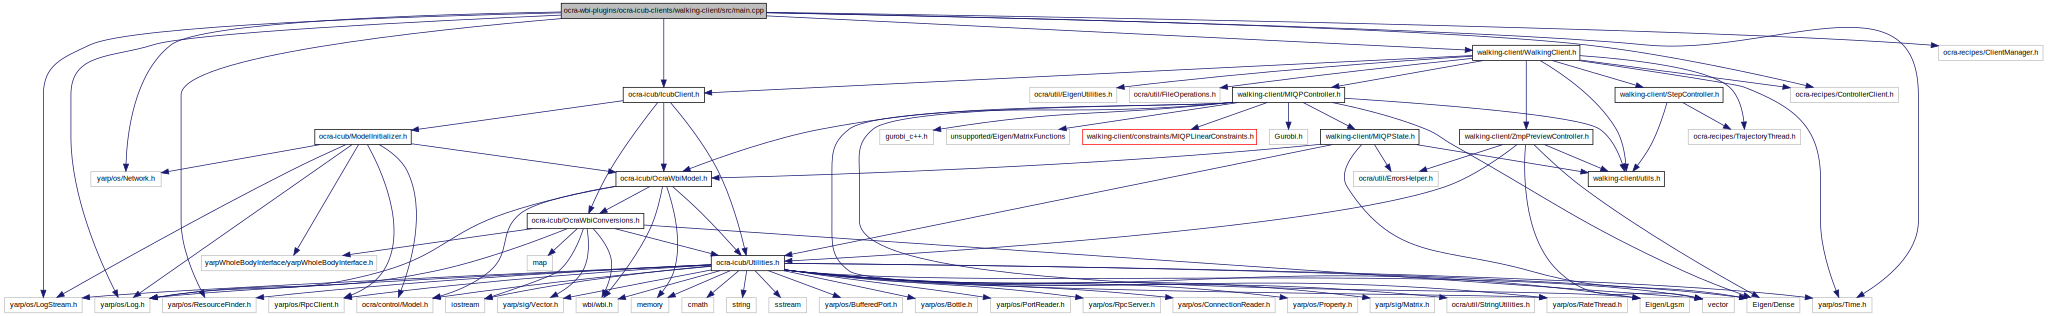
\includegraphics[width=350pt]{ocra-icub-clients_2walking-client_2src_2main_8cpp__incl}
\end{center}
\end{figure}
\subsection*{\-Functions}
\begin{DoxyCompactItemize}
\item 
int \hyperlink{ocra-icub-clients_2walking-client_2src_2main_8cpp_a0ddf1224851353fc92bfbff6f499fa97}{main} (int argc, char $\ast$argv\mbox{[}$\,$\mbox{]})
\end{DoxyCompactItemize}


\subsection{\-Function \-Documentation}
\hypertarget{ocra-icub-clients_2walking-client_2src_2main_8cpp_a0ddf1224851353fc92bfbff6f499fa97}{\index{ocra-\/icub-\/clients/walking-\/client/src/main.\-cpp@{ocra-\/icub-\/clients/walking-\/client/src/main.\-cpp}!main@{main}}
\index{main@{main}!ocra-icub-clients/walking-client/src/main.cpp@{ocra-\/icub-\/clients/walking-\/client/src/main.\-cpp}}
\subsubsection[{main}]{\setlength{\rightskip}{0pt plus 5cm}int {\bf main} (
\begin{DoxyParamCaption}
\item[{int}]{argc, }
\item[{char $\ast$}]{argv\mbox{[}$\,$\mbox{]}}
\end{DoxyParamCaption}
)}}\label{ocra-icub-clients_2walking-client_2src_2main_8cpp_a0ddf1224851353fc92bfbff6f499fa97}

\hypertarget{Module_8cpp}{\section{ocra-\/wbi-\/plugins/ocra-\/icub-\/server/src/\-Module.cpp \-File \-Reference}
\label{Module_8cpp}\index{ocra-\/wbi-\/plugins/ocra-\/icub-\/server/src/\-Module.\-cpp@{ocra-\/wbi-\/plugins/ocra-\/icub-\/server/src/\-Module.\-cpp}}
}
{\ttfamily \#include \char`\"{}ocra-\/icub-\/server/\-Module.\-h\char`\"{}}\*
\-Include dependency graph for \-Module.\-cpp\-:\nopagebreak
\begin{figure}[H]
\begin{center}
\leavevmode
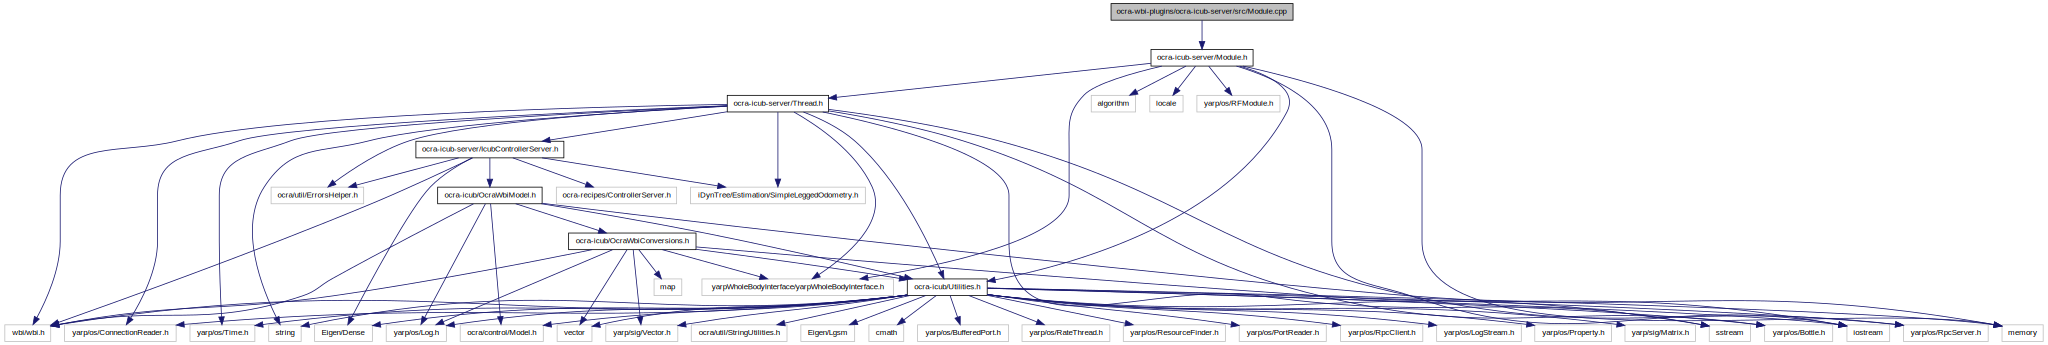
\includegraphics[width=350pt]{Module_8cpp__incl}
\end{center}
\end{figure}

\hypertarget{Thread_8cpp}{\section{ocra-\/wbi-\/plugins/ocra-\/icub-\/server/src/\-Thread.cpp \-File \-Reference}
\label{Thread_8cpp}\index{ocra-\/wbi-\/plugins/ocra-\/icub-\/server/src/\-Thread.\-cpp@{ocra-\/wbi-\/plugins/ocra-\/icub-\/server/src/\-Thread.\-cpp}}
}


\-The thread class for the controller server.  


{\ttfamily \#include \char`\"{}ocra-\/icub-\/server/\-Thread.\-h\char`\"{}}\*
\-Include dependency graph for \-Thread.\-cpp\-:
\nopagebreak
\begin{figure}[H]
\begin{center}
\leavevmode
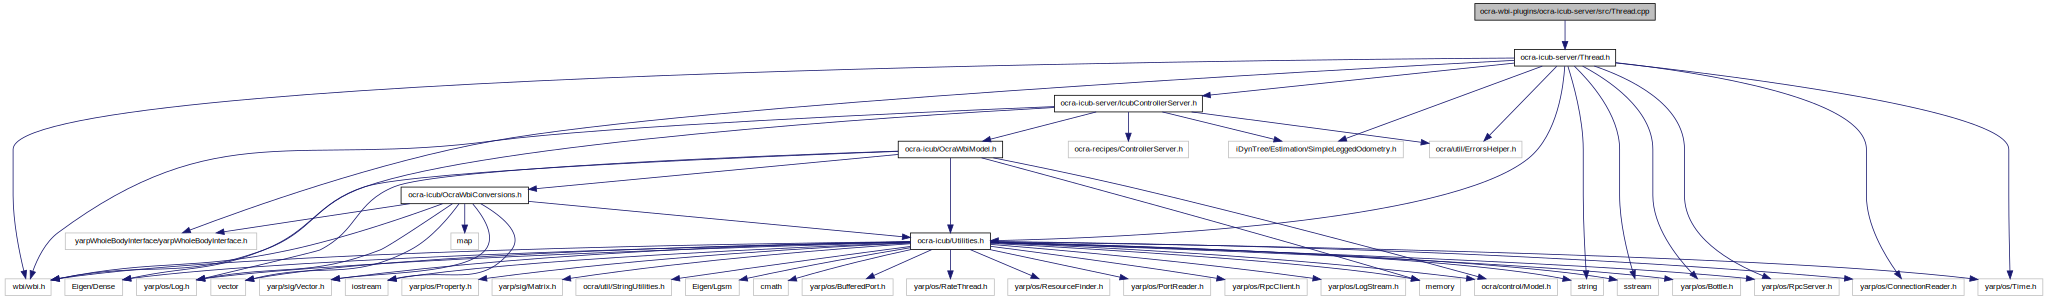
\includegraphics[width=350pt]{Thread_8cpp__incl}
\end{center}
\end{figure}
\subsection*{\-Functions}
\begin{DoxyCompactItemize}
\item 
std\-::ostream \& \hyperlink{Thread_8cpp_a30ab3a18ec4f8101aa6f1df6926888f6}{operator$<$$<$} (std\-::ostream \&out, const \hyperlink{classOcraControllerOptions}{\-Ocra\-Controller\-Options} \&opts)
\end{DoxyCompactItemize}


\subsection{\-Detailed \-Description}
\-The thread class for the controller server. \begin{DoxyAuthor}{\-Author}
\mbox{[}\-Ryan \-Lober\mbox{]}(\href{http://www.ryanlober.com}{\tt http\-://www.\-ryanlober.\-com}) 

\mbox{[}\-Antoine \-Hoarau\mbox{]}(\href{http://ahoarau.github.io}{\tt http\-://ahoarau.\-github.\-io}) 
\end{DoxyAuthor}
\begin{DoxyDate}{\-Date}
\-Feb 2016 
\end{DoxyDate}
\begin{DoxyCopyright}{\-Copyright}
\-G\-N\-U \-General \-Public \-License. 
\end{DoxyCopyright}


\subsection{\-Function \-Documentation}
\hypertarget{Thread_8cpp_a30ab3a18ec4f8101aa6f1df6926888f6}{\index{\-Thread.\-cpp@{\-Thread.\-cpp}!operator$<$$<$@{operator$<$$<$}}
\index{operator$<$$<$@{operator$<$$<$}!Thread.cpp@{\-Thread.\-cpp}}
\subsubsection[{operator$<$$<$}]{\setlength{\rightskip}{0pt plus 5cm}std\-::ostream\& operator$<$$<$ (
\begin{DoxyParamCaption}
\item[{std\-::ostream \&}]{out, }
\item[{const {\bf \-Ocra\-Controller\-Options} \&}]{opts}
\end{DoxyParamCaption}
)}}\label{Thread_8cpp_a30ab3a18ec4f8101aa6f1df6926888f6}

\hypertarget{IcubClient_8h}{\section{ocra-\/wbi-\/plugins/ocra-\/icub/include/ocra-\/icub/\-Icub\-Client.h \-File \-Reference}
\label{IcubClient_8h}\index{ocra-\/wbi-\/plugins/ocra-\/icub/include/ocra-\/icub/\-Icub\-Client.\-h@{ocra-\/wbi-\/plugins/ocra-\/icub/include/ocra-\/icub/\-Icub\-Client.\-h}}
}
{\ttfamily \#include $<$ocra-\/icub/\-Model\-Initializer.\-h$>$}\*
{\ttfamily \#include $<$ocra-\/icub/\-Ocra\-Wbi\-Conversions.\-h$>$}\*
{\ttfamily \#include $<$ocra-\/icub/\-Ocra\-Wbi\-Model.\-h$>$}\*
{\ttfamily \#include $<$ocra-\/icub/\-Utilities.\-h$>$}\*
\-Include dependency graph for \-Icub\-Client.\-h\-:
\nopagebreak
\begin{figure}[H]
\begin{center}
\leavevmode
\includegraphics[width=350pt]{IcubClient_8h__incl}
\end{center}
\end{figure}
\-This graph shows which files directly or indirectly include this file\-:
\nopagebreak
\begin{figure}[H]
\begin{center}
\leavevmode
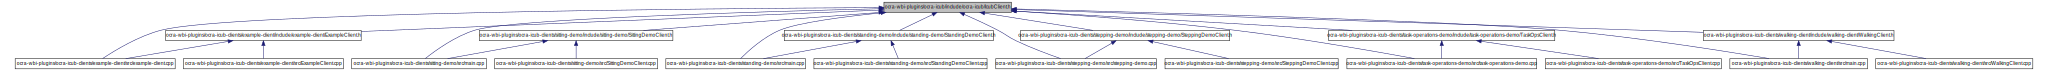
\includegraphics[width=350pt]{IcubClient_8h__dep__incl}
\end{center}
\end{figure}

\hypertarget{ModelInitializer_8h}{\section{ocra-\/wbi-\/plugins/ocra-\/icub/include/ocra-\/icub/\-Model\-Initializer.h \-File \-Reference}
\label{ModelInitializer_8h}\index{ocra-\/wbi-\/plugins/ocra-\/icub/include/ocra-\/icub/\-Model\-Initializer.\-h@{ocra-\/wbi-\/plugins/ocra-\/icub/include/ocra-\/icub/\-Model\-Initializer.\-h}}
}
{\ttfamily \#include $<$ocra-\/icub/\-Ocra\-Wbi\-Model.\-h$>$}\*
{\ttfamily \#include $<$ocra/control/\-Model.\-h$>$}\*
{\ttfamily \#include $<$yarp\-Whole\-Body\-Interface/yarp\-Whole\-Body\-Interface.\-h$>$}\*
{\ttfamily \#include $<$yarp/os/\-Rpc\-Client.\-h$>$}\*
{\ttfamily \#include $<$yarp/os/\-Network.\-h$>$}\*
{\ttfamily \#include $<$yarp/os/\-Log\-Stream.\-h$>$}\*
{\ttfamily \#include $<$yarp/os/\-Log.\-h$>$}\*
\-Include dependency graph for \-Model\-Initializer.\-h\-:\nopagebreak
\begin{figure}[H]
\begin{center}
\leavevmode
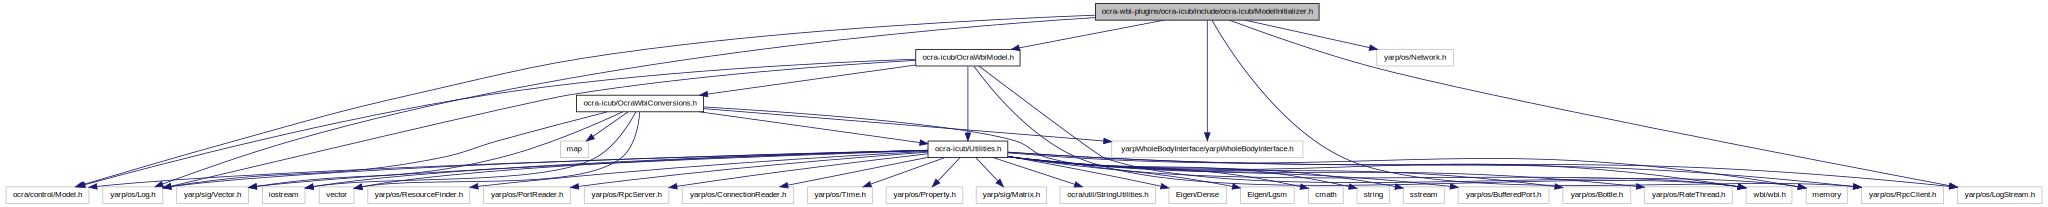
\includegraphics[width=350pt]{ModelInitializer_8h__incl}
\end{center}
\end{figure}
\-This graph shows which files directly or indirectly include this file\-:\nopagebreak
\begin{figure}[H]
\begin{center}
\leavevmode
\includegraphics[width=350pt]{ModelInitializer_8h__dep__incl}
\end{center}
\end{figure}
\subsection*{\-Classes}
\begin{DoxyCompactItemize}
\item 
class \hyperlink{classocra__icub_1_1ModelInitializer}{ocra\-\_\-icub\-::\-Model\-Initializer}
\end{DoxyCompactItemize}
\subsection*{\-Namespaces}
\begin{DoxyCompactItemize}
\item 
namespace \hyperlink{namespaceocra__icub}{ocra\-\_\-icub}
\end{DoxyCompactItemize}

\hypertarget{OcraWbiConversions_8h}{\section{ocra-\/wbi-\/plugins/ocra-\/icub/include/ocra-\/icub/\-Ocra\-Wbi\-Conversions.h \-File \-Reference}
\label{OcraWbiConversions_8h}\index{ocra-\/wbi-\/plugins/ocra-\/icub/include/ocra-\/icub/\-Ocra\-Wbi\-Conversions.\-h@{ocra-\/wbi-\/plugins/ocra-\/icub/include/ocra-\/icub/\-Ocra\-Wbi\-Conversions.\-h}}
}


\-A utility class full of static conversion functions.  


{\ttfamily \#include $<$iostream$>$}\*
{\ttfamily \#include $<$map$>$}\*
{\ttfamily \#include $<$vector$>$}\*
{\ttfamily \#include $<$yarp/sig/\-Vector.\-h$>$}\*
{\ttfamily \#include $<$yarp/os/\-Log.\-h$>$}\*
{\ttfamily \#include $<$wbi/wbi.\-h$>$}\*
{\ttfamily \#include $<$yarp\-Whole\-Body\-Interface/yarp\-Whole\-Body\-Interface.\-h$>$}\*
{\ttfamily \#include \char`\"{}ocra-\/icub/\-Utilities.\-h\char`\"{}}\*
\-Include dependency graph for \-Ocra\-Wbi\-Conversions.\-h\-:\nopagebreak
\begin{figure}[H]
\begin{center}
\leavevmode
\includegraphics[width=350pt]{OcraWbiConversions_8h__incl}
\end{center}
\end{figure}
\-This graph shows which files directly or indirectly include this file\-:
\nopagebreak
\begin{figure}[H]
\begin{center}
\leavevmode
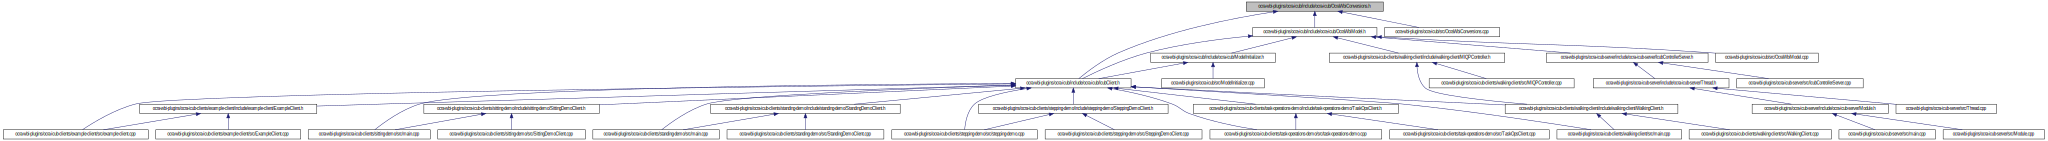
\includegraphics[width=350pt]{OcraWbiConversions_8h__dep__incl}
\end{center}
\end{figure}
\subsection*{\-Classes}
\begin{DoxyCompactItemize}
\item 
class \hyperlink{classocra__icub_1_1OcraWbiConversions}{ocra\-\_\-icub\-::\-Ocra\-Wbi\-Conversions}
\end{DoxyCompactItemize}
\subsection*{\-Namespaces}
\begin{DoxyCompactItemize}
\item 
namespace \hyperlink{namespaceocra__icub}{ocra\-\_\-icub}
\end{DoxyCompactItemize}
\subsection*{\-Typedefs}
\begin{DoxyCompactItemize}
\item 
typedef \-Eigen\-::\-Matrix$<$ double, \*
\-Eigen\-::\-Dynamic, \-Eigen\-::\-Dynamic, \*
\-Eigen\-::\-Row\-Major $>$ \hyperlink{namespaceocra__icub_aa5e36a19ed031c28ca83c207bd7dd83f}{ocra\-\_\-icub\-::\-Matrix\-Xd\-Rm}
\end{DoxyCompactItemize}


\subsection{\-Detailed \-Description}
\-A utility class full of static conversion functions. \begin{DoxyAuthor}{\-Author}
\mbox{[}\-Ryan \-Lober\mbox{]}(\href{http://www.ryanlober.com}{\tt http\-://www.\-ryanlober.\-com}) 

\mbox{[}\-Antoine \-Hoarau\mbox{]}(\href{http://ahoarau.github.io}{\tt http\-://ahoarau.\-github.\-io}) 
\end{DoxyAuthor}
\begin{DoxyDate}{\-Date}
\-Feb 2016 
\end{DoxyDate}
\begin{DoxyCopyright}{\-Copyright}
\-G\-N\-U \-General \-Public \-License. 
\end{DoxyCopyright}

\hypertarget{OcraWbiModel_8h}{\section{ocra-\/wbi-\/plugins/ocra-\/icub/include/ocra-\/icub/\-Ocra\-Wbi\-Model.h \-File \-Reference}
\label{OcraWbiModel_8h}\index{ocra-\/wbi-\/plugins/ocra-\/icub/include/ocra-\/icub/\-Ocra\-Wbi\-Model.\-h@{ocra-\/wbi-\/plugins/ocra-\/icub/include/ocra-\/icub/\-Ocra\-Wbi\-Model.\-h}}
}


\-Implementation of ocra\-::\-Model using whole\-Body\-Interface.  


{\ttfamily \#include $<$memory$>$}\*
{\ttfamily \#include \char`\"{}ocra/control/\-Model.\-h\char`\"{}}\*
{\ttfamily \#include $<$wbi/wbi.\-h$>$}\*
{\ttfamily \#include $<$yarp/os/\-Log.\-h$>$}\*
{\ttfamily \#include \char`\"{}ocra-\/icub/\-Ocra\-Wbi\-Conversions.\-h\char`\"{}}\*
{\ttfamily \#include \char`\"{}ocra-\/icub/\-Utilities.\-h\char`\"{}}\*
\-Include dependency graph for \-Ocra\-Wbi\-Model.\-h\-:\nopagebreak
\begin{figure}[H]
\begin{center}
\leavevmode
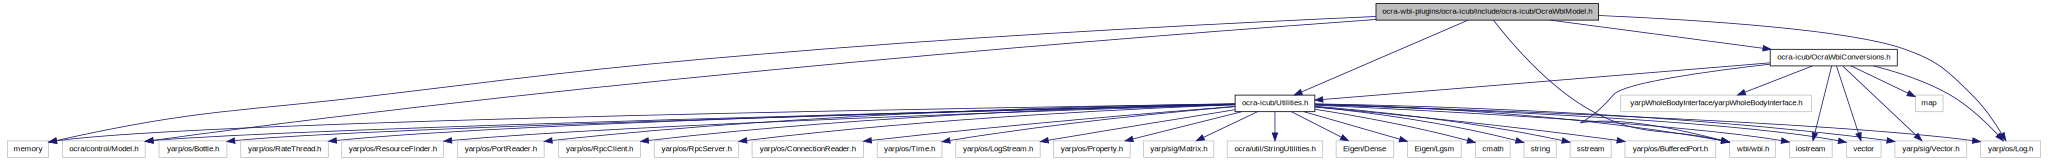
\includegraphics[width=350pt]{OcraWbiModel_8h__incl}
\end{center}
\end{figure}
\-This graph shows which files directly or indirectly include this file\-:\nopagebreak
\begin{figure}[H]
\begin{center}
\leavevmode
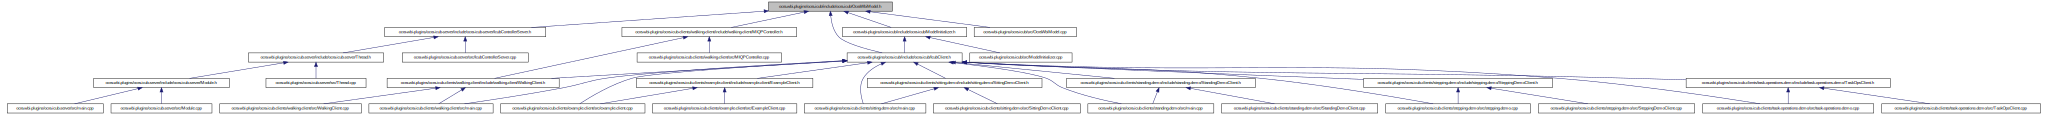
\includegraphics[width=350pt]{OcraWbiModel_8h__dep__incl}
\end{center}
\end{figure}
\subsection*{\-Classes}
\begin{DoxyCompactItemize}
\item 
class \hyperlink{classocra__icub_1_1OcraWbiModel}{ocra\-\_\-icub\-::\-Ocra\-Wbi\-Model}
\end{DoxyCompactItemize}
\subsection*{\-Namespaces}
\begin{DoxyCompactItemize}
\item 
namespace \hyperlink{namespaceocra__icub}{ocra\-\_\-icub}
\end{DoxyCompactItemize}


\subsection{\-Detailed \-Description}
\-Implementation of ocra\-::\-Model using whole\-Body\-Interface. \begin{DoxyAuthor}{\-Author}
\mbox{[}\-Ryan \-Lober\mbox{]}(\href{http://www.ryanlober.com}{\tt http\-://www.\-ryanlober.\-com}) 

\mbox{[}\-Antoine \-Hoarau\mbox{]}(\href{http://ahoarau.github.io}{\tt http\-://ahoarau.\-github.\-io}) 
\end{DoxyAuthor}
\begin{DoxyDate}{\-Date}
\-Feb 2016 
\end{DoxyDate}
\begin{DoxyCopyright}{\-Copyright}
\-G\-N\-U \-General \-Public \-License. 
\end{DoxyCopyright}

\hypertarget{Utilities_8h}{\section{ocra-\/wbi-\/plugins/ocra-\/icub/include/ocra-\/icub/\-Utilities.h \-File \-Reference}
\label{Utilities_8h}\index{ocra-\/wbi-\/plugins/ocra-\/icub/include/ocra-\/icub/\-Utilities.\-h@{ocra-\/wbi-\/plugins/ocra-\/icub/include/ocra-\/icub/\-Utilities.\-h}}
}


\-Some useful tools for the ocra-\/icub lib.  


{\ttfamily \#include $<$memory$>$}\*
{\ttfamily \#include $<$cmath$>$}\*
{\ttfamily \#include $<$iostream$>$}\*
{\ttfamily \#include $<$string$>$}\*
{\ttfamily \#include $<$vector$>$}\*
{\ttfamily \#include $<$sstream$>$}\*
{\ttfamily \#include $<$yarp/os/\-Buffered\-Port.\-h$>$}\*
{\ttfamily \#include $<$yarp/os/\-Bottle.\-h$>$}\*
{\ttfamily \#include $<$yarp/os/\-Rate\-Thread.\-h$>$}\*
{\ttfamily \#include $<$yarp/os/\-Resource\-Finder.\-h$>$}\*
{\ttfamily \#include $<$yarp/os/\-Port\-Reader.\-h$>$}\*
{\ttfamily \#include $<$yarp/os/\-Rpc\-Client.\-h$>$}\*
{\ttfamily \#include $<$yarp/os/\-Rpc\-Server.\-h$>$}\*
{\ttfamily \#include $<$yarp/os/\-Connection\-Reader.\-h$>$}\*
{\ttfamily \#include $<$yarp/os/\-Time.\-h$>$}\*
{\ttfamily \#include $<$yarp/os/\-Log.\-h$>$}\*
{\ttfamily \#include $<$yarp/os/\-Log\-Stream.\-h$>$}\*
{\ttfamily \#include $<$yarp/os/\-Property.\-h$>$}\*
{\ttfamily \#include $<$yarp/sig/\-Vector.\-h$>$}\*
{\ttfamily \#include $<$yarp/sig/\-Matrix.\-h$>$}\*
{\ttfamily \#include $<$wbi/wbi.\-h$>$}\*
{\ttfamily \#include \char`\"{}ocra/control/\-Model.\-h\char`\"{}}\*
{\ttfamily \#include \char`\"{}ocra/util/\-String\-Utilities.\-h\char`\"{}}\*
{\ttfamily \#include $<$\-Eigen/\-Dense$>$}\*
{\ttfamily \#include $<$\-Eigen/\-Lgsm$>$}\*
\-Include dependency graph for \-Utilities.\-h\-:\nopagebreak
\begin{figure}[H]
\begin{center}
\leavevmode
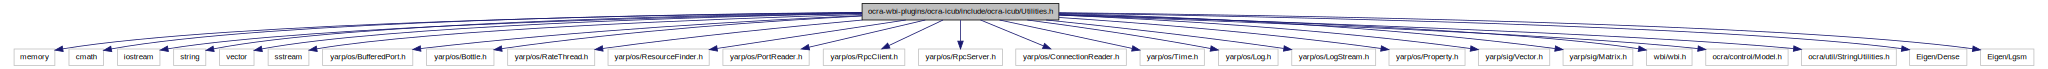
\includegraphics[width=350pt]{Utilities_8h__incl}
\end{center}
\end{figure}
\-This graph shows which files directly or indirectly include this file\-:\nopagebreak
\begin{figure}[H]
\begin{center}
\leavevmode
\includegraphics[width=350pt]{Utilities_8h__dep__incl}
\end{center}
\end{figure}
\subsection*{\-Namespaces}
\begin{DoxyCompactItemize}
\item 
namespace \hyperlink{namespaceocra__icub}{ocra\-\_\-icub}
\end{DoxyCompactItemize}
\subsection*{\-Defines}
\begin{DoxyCompactItemize}
\item 
\#define \hyperlink{Utilities_8h_a986e6d54948ebf3007dc52bd0fc737be}{\-C\-L\-A\-S\-S\-\_\-\-P\-O\-I\-N\-T\-E\-R\-\_\-\-T\-Y\-P\-E\-D\-E\-F\-S}(\-Class)
\end{DoxyCompactItemize}
\subsection*{\-Enumerations}
\begin{DoxyCompactItemize}
\item 
enum \hyperlink{namespaceocra__icub_afbd2db66b68005fb7cfac19210caf83f}{ocra\-\_\-icub\-::\-O\-C\-R\-A\-\_\-\-I\-C\-U\-B\-\_\-\-M\-E\-S\-S\-A\-G\-E} \{ \*
\hyperlink{namespaceocra__icub_afbd2db66b68005fb7cfac19210caf83fafa982af27b4e13f109d8769472d75217}{ocra\-\_\-icub\-::\-S\-T\-R\-I\-N\-G\-\_\-\-M\-E\-S\-S\-A\-G\-E} =  -\/1, 
\hyperlink{namespaceocra__icub_afbd2db66b68005fb7cfac19210caf83faa0c1832978fad84ef108d48265af68d2}{ocra\-\_\-icub\-::\-F\-A\-I\-L\-U\-R\-E} =  0, 
\hyperlink{namespaceocra__icub_afbd2db66b68005fb7cfac19210caf83fa67c96e3afcb39533f69c97dc5e9734e5}{ocra\-\_\-icub\-::\-S\-U\-C\-C\-E\-S\-S}, 
\hyperlink{namespaceocra__icub_afbd2db66b68005fb7cfac19210caf83fae8fe02f5f3b1b11d4749e720b9ec3636}{ocra\-\_\-icub\-::\-G\-E\-T\-\_\-\-M\-O\-D\-E\-L\-\_\-\-C\-O\-N\-F\-I\-G\-\_\-\-I\-N\-F\-O}, 
\*
\hyperlink{namespaceocra__icub_afbd2db66b68005fb7cfac19210caf83fa772ab917d1ff28db029af9271208a69a}{ocra\-\_\-icub\-::\-G\-E\-T\-\_\-\-C\-O\-N\-T\-R\-O\-L\-L\-E\-R\-\_\-\-S\-E\-R\-V\-E\-R\-\_\-\-S\-T\-A\-T\-U\-S}, 
\hyperlink{namespaceocra__icub_afbd2db66b68005fb7cfac19210caf83fa5dee3cfa0ab6c29f5546bc9e30c0aef5}{ocra\-\_\-icub\-::\-C\-O\-N\-T\-R\-O\-L\-L\-E\-R\-\_\-\-S\-E\-R\-V\-E\-R\-\_\-\-R\-U\-N\-N\-I\-N\-G}, 
\hyperlink{namespaceocra__icub_afbd2db66b68005fb7cfac19210caf83fafd31e40d18e553fc09105d360455bc49}{ocra\-\_\-icub\-::\-C\-O\-N\-T\-R\-O\-L\-L\-E\-R\-\_\-\-S\-E\-R\-V\-E\-R\-\_\-\-S\-T\-O\-P\-P\-E\-D}, 
\hyperlink{namespaceocra__icub_afbd2db66b68005fb7cfac19210caf83fa48ad7962d035a58257a0381872ce27b1}{ocra\-\_\-icub\-::\-C\-O\-N\-T\-R\-O\-L\-L\-E\-R\-\_\-\-S\-E\-R\-V\-E\-R\-\_\-\-P\-A\-U\-S\-E\-D}, 
\*
\hyperlink{namespaceocra__icub_afbd2db66b68005fb7cfac19210caf83fafd78d107914396f475c3b12d2b31ea2a}{ocra\-\_\-icub\-::\-G\-E\-T\-\_\-\-L\-\_\-\-F\-O\-O\-T\-\_\-\-P\-O\-S\-E}, 
\hyperlink{namespaceocra__icub_afbd2db66b68005fb7cfac19210caf83fae7c9fa2563b6c0b14e5b05d1794dac36}{ocra\-\_\-icub\-::\-H\-E\-L\-P}
 \}
\end{DoxyCompactItemize}
\subsection*{\-Functions}
\begin{DoxyCompactItemize}
\item 
void \hyperlink{namespaceocra__icub_a07ffe33877389b6b111944e8a666e221}{ocra\-\_\-icub\-::get\-Nominal\-Posture} (const ocra\-::\-Model \&model, \-Eigen\-::\-Vector\-Xd \&q)
\item 
void \hyperlink{namespaceocra__icub_a91c3caf94014ea9988e56dd2572768ce}{ocra\-\_\-icub\-::get\-Home\-Posture} (const ocra\-::\-Model \&model, \-Eigen\-::\-Vector\-Xd \&q)
\end{DoxyCompactItemize}
\subsection*{\-Variables}
\begin{DoxyCompactItemize}
\item 
static constexpr double \hyperlink{namespaceocra__icub_ab06477ded34ed5514b911a3511b22e3d}{ocra\-\_\-icub\-::\-D\-E\-G\-\_\-\-T\-O\-\_\-\-R\-A\-D} = \-M\-\_\-\-P\-I/180.\-0
\end{DoxyCompactItemize}


\subsection{\-Detailed \-Description}
\-Some useful tools for the ocra-\/icub lib. \-This file is for all the various macros and helper classes that are generic to ocra-\/icub. \-It is also a place for all the repeated includes like standard stl includes etc. \begin{DoxyAuthor}{\-Author}
\mbox{[}\-Ryan \-Lober\mbox{]}(\href{http://www.ryanlober.com}{\tt http\-://www.\-ryanlober.\-com}) 
\end{DoxyAuthor}
\begin{DoxyDate}{\-Date}
\-Feb 2016 
\end{DoxyDate}
\begin{DoxyCopyright}{\-Copyright}
\-G\-N\-U \-General \-Public \-License. 
\end{DoxyCopyright}


\subsection{\-Define \-Documentation}
\hypertarget{Utilities_8h_a986e6d54948ebf3007dc52bd0fc737be}{\index{\-Utilities.\-h@{\-Utilities.\-h}!\-C\-L\-A\-S\-S\-\_\-\-P\-O\-I\-N\-T\-E\-R\-\_\-\-T\-Y\-P\-E\-D\-E\-F\-S@{\-C\-L\-A\-S\-S\-\_\-\-P\-O\-I\-N\-T\-E\-R\-\_\-\-T\-Y\-P\-E\-D\-E\-F\-S}}
\index{\-C\-L\-A\-S\-S\-\_\-\-P\-O\-I\-N\-T\-E\-R\-\_\-\-T\-Y\-P\-E\-D\-E\-F\-S@{\-C\-L\-A\-S\-S\-\_\-\-P\-O\-I\-N\-T\-E\-R\-\_\-\-T\-Y\-P\-E\-D\-E\-F\-S}!Utilities.h@{\-Utilities.\-h}}
\subsubsection[{\-C\-L\-A\-S\-S\-\_\-\-P\-O\-I\-N\-T\-E\-R\-\_\-\-T\-Y\-P\-E\-D\-E\-F\-S}]{\setlength{\rightskip}{0pt plus 5cm}\#define {\bf \-C\-L\-A\-S\-S\-\_\-\-P\-O\-I\-N\-T\-E\-R\-\_\-\-T\-Y\-P\-E\-D\-E\-F\-S}(
\begin{DoxyParamCaption}
\item[{}]{\-Class}
\end{DoxyParamCaption}
)}}\label{Utilities_8h_a986e6d54948ebf3007dc52bd0fc737be}
{\bfseries \-Value\-:}
\begin{DoxyCode}
public:\
using ptr           = std::shared_ptr   <Class>;  \
using shared_ptr    = std::shared_ptr   <Class>;  \
using unique_ptr    = std::unique_ptr   <Class>;  \
using weak_ptr      = std::weak_ptr     <Class>;  \
using const_ptr           = const std::shared_ptr   <Class>;  \
using const_shared_ptr    = const std::shared_ptr   <Class>;  \
using const_unique_ptr    = const std::unique_ptr   <Class>;  \
using const_weak_ptr      = const std::weak_ptr     <Class>;
\end{DoxyCode}
\-Macro function which basically just defines pointer typdefs for classes. \-Note that normally macros are evil monsters but \-I think this is a perfect usage case to cut down on repeated code. 
\begin{DoxyParams}{\-Parameters}
{\em \-Class} & \-Just pop this bad boy below the class definition and it will do the rest. \\
\hline
\end{DoxyParams}

\hypertarget{ModelInitializer_8cpp}{\section{ocra-\/wbi-\/plugins/ocra-\/icub/src/\-Model\-Initializer.cpp \-File \-Reference}
\label{ModelInitializer_8cpp}\index{ocra-\/wbi-\/plugins/ocra-\/icub/src/\-Model\-Initializer.\-cpp@{ocra-\/wbi-\/plugins/ocra-\/icub/src/\-Model\-Initializer.\-cpp}}
}
{\ttfamily \#include $<$ocra-\/icub/\-Model\-Initializer.\-h$>$}\*
\-Include dependency graph for \-Model\-Initializer.\-cpp\-:
\nopagebreak
\begin{figure}[H]
\begin{center}
\leavevmode
\includegraphics[width=350pt]{ModelInitializer_8cpp__incl}
\end{center}
\end{figure}

\hypertarget{OcraWbiConversions_8cpp}{\section{ocra-\/wbi-\/plugins/ocra-\/icub/src/\-Ocra\-Wbi\-Conversions.cpp \-File \-Reference}
\label{OcraWbiConversions_8cpp}\index{ocra-\/wbi-\/plugins/ocra-\/icub/src/\-Ocra\-Wbi\-Conversions.\-cpp@{ocra-\/wbi-\/plugins/ocra-\/icub/src/\-Ocra\-Wbi\-Conversions.\-cpp}}
}


\-A utility class full of static conversion functions.  


{\ttfamily \#include $<$ocra-\/icub/\-Ocra\-Wbi\-Conversions.\-h$>$}\*
\-Include dependency graph for \-Ocra\-Wbi\-Conversions.\-cpp\-:\nopagebreak
\begin{figure}[H]
\begin{center}
\leavevmode
\includegraphics[width=350pt]{OcraWbiConversions_8cpp__incl}
\end{center}
\end{figure}


\subsection{\-Detailed \-Description}
\-A utility class full of static conversion functions. \begin{DoxyAuthor}{\-Author}
\mbox{[}\-Ryan \-Lober\mbox{]}(\href{http://www.ryanlober.com}{\tt http\-://www.\-ryanlober.\-com}) 

\mbox{[}\-Antoine \-Hoarau\mbox{]}(\href{http://ahoarau.github.io}{\tt http\-://ahoarau.\-github.\-io}) 
\end{DoxyAuthor}
\begin{DoxyDate}{\-Date}
\-Feb 2016 
\end{DoxyDate}
\begin{DoxyCopyright}{\-Copyright}
\-G\-N\-U \-General \-Public \-License. 
\end{DoxyCopyright}

\hypertarget{OcraWbiModel_8cpp}{\section{ocra-\/wbi-\/plugins/ocra-\/icub/src/\-Ocra\-Wbi\-Model.cpp \-File \-Reference}
\label{OcraWbiModel_8cpp}\index{ocra-\/wbi-\/plugins/ocra-\/icub/src/\-Ocra\-Wbi\-Model.\-cpp@{ocra-\/wbi-\/plugins/ocra-\/icub/src/\-Ocra\-Wbi\-Model.\-cpp}}
}


\-Implementation of ocra\-::\-Model using whole\-Body\-Interface.  


{\ttfamily \#include $<$ocra-\/icub/\-Ocra\-Wbi\-Model.\-h$>$}\*
\-Include dependency graph for \-Ocra\-Wbi\-Model.\-cpp\-:\nopagebreak
\begin{figure}[H]
\begin{center}
\leavevmode
\includegraphics[width=350pt]{OcraWbiModel_8cpp__incl}
\end{center}
\end{figure}
\subsection*{\-Classes}
\begin{DoxyCompactItemize}
\item 
struct \hyperlink{structOcraWbiModel_1_1OcraWbiModel__pimpl}{ocra\-\_\-icub\-::\-Ocra\-Wbi\-Model\-::\-Ocra\-Wbi\-Model\-\_\-pimpl}
\end{DoxyCompactItemize}
\subsection*{\-Defines}
\begin{DoxyCompactItemize}
\item 
\#define \hyperlink{OcraWbiModel_8cpp_a7f4e728fa0fd89911a2c60c42c0d4560}{\-A\-L\-L\-\_\-\-J\-O\-I\-N\-T\-S}~-\/1
\item 
\#define \hyperlink{OcraWbiModel_8cpp_a29de1200631802e23f75bbd14adcc082}{\-F\-R\-E\-E\-\_\-\-R\-O\-O\-T\-\_\-\-D\-O\-F}~6
\item 
\#define \hyperlink{OcraWbiModel_8cpp_a72cb22de2538ae949cc73fa3d7c33bdc}{\-C\-O\-M\-\_\-\-P\-O\-S\-\_\-\-D\-I\-M}~3
\item 
\#define \hyperlink{OcraWbiModel_8cpp_ab4a87cb824ceff256c6b8bce7701af58}{\-T\-R\-A\-N\-S\-\_\-\-R\-O\-T\-\_\-\-D\-I\-M}~6
\item 
\#define \hyperlink{OcraWbiModel_8cpp_afbb98f526272c46369f405eee4e9d9aa}{\-G\-R\-A\-V\-I\-T\-Y\-\_\-\-C\-O\-N\-S\-T\-A\-N\-T}~-\/9.\-81
\end{DoxyCompactItemize}
\subsection*{\-Typedefs}
\begin{DoxyCompactItemize}
\item 
typedef \*
\hyperlink{OcraWbiModel_8cpp_a2ee3f7feea423a8bc6b8fbcea1d4e217}{\-Eigen\-::\-Displacementd\-::\-Adjoint\-Matrix} \hyperlink{OcraWbiModel_8cpp_a2ee3f7feea423a8bc6b8fbcea1d4e217}{\-Adjoint\-Matrix}
\end{DoxyCompactItemize}
\subsection*{\-Variables}
\begin{DoxyCompactItemize}
\item 
const double \hyperlink{OcraWbiModel_8cpp_a3cdc4ec85b339c11e5b34ce069bf7077}{g\-\_\-vector} \mbox{[}3\mbox{]} = \{0, 0, \hyperlink{OcraWbiModel_8cpp_afbb98f526272c46369f405eee4e9d9aa}{\-G\-R\-A\-V\-I\-T\-Y\-\_\-\-C\-O\-N\-S\-T\-A\-N\-T}\}
\end{DoxyCompactItemize}


\subsection{\-Detailed \-Description}
\-Implementation of ocra\-::\-Model using whole\-Body\-Interface. \begin{DoxyAuthor}{\-Author}
\mbox{[}\-Ryan \-Lober\mbox{]}(\href{http://www.ryanlober.com}{\tt http\-://www.\-ryanlober.\-com}) 

\mbox{[}\-Antoine \-Hoarau\mbox{]}(\href{http://ahoarau.github.io}{\tt http\-://ahoarau.\-github.\-io}) 
\end{DoxyAuthor}
\begin{DoxyDate}{\-Date}
\-Feb 2016 
\end{DoxyDate}
\begin{DoxyCopyright}{\-Copyright}
\-G\-N\-U \-General \-Public \-License. 
\end{DoxyCopyright}


\subsection{\-Define \-Documentation}
\hypertarget{OcraWbiModel_8cpp_a7f4e728fa0fd89911a2c60c42c0d4560}{\index{\-Ocra\-Wbi\-Model.\-cpp@{\-Ocra\-Wbi\-Model.\-cpp}!\-A\-L\-L\-\_\-\-J\-O\-I\-N\-T\-S@{\-A\-L\-L\-\_\-\-J\-O\-I\-N\-T\-S}}
\index{\-A\-L\-L\-\_\-\-J\-O\-I\-N\-T\-S@{\-A\-L\-L\-\_\-\-J\-O\-I\-N\-T\-S}!OcraWbiModel.cpp@{\-Ocra\-Wbi\-Model.\-cpp}}
\subsubsection[{\-A\-L\-L\-\_\-\-J\-O\-I\-N\-T\-S}]{\setlength{\rightskip}{0pt plus 5cm}\#define {\bf \-A\-L\-L\-\_\-\-J\-O\-I\-N\-T\-S}~-\/1}}\label{OcraWbiModel_8cpp_a7f4e728fa0fd89911a2c60c42c0d4560}
\hypertarget{OcraWbiModel_8cpp_a72cb22de2538ae949cc73fa3d7c33bdc}{\index{\-Ocra\-Wbi\-Model.\-cpp@{\-Ocra\-Wbi\-Model.\-cpp}!\-C\-O\-M\-\_\-\-P\-O\-S\-\_\-\-D\-I\-M@{\-C\-O\-M\-\_\-\-P\-O\-S\-\_\-\-D\-I\-M}}
\index{\-C\-O\-M\-\_\-\-P\-O\-S\-\_\-\-D\-I\-M@{\-C\-O\-M\-\_\-\-P\-O\-S\-\_\-\-D\-I\-M}!OcraWbiModel.cpp@{\-Ocra\-Wbi\-Model.\-cpp}}
\subsubsection[{\-C\-O\-M\-\_\-\-P\-O\-S\-\_\-\-D\-I\-M}]{\setlength{\rightskip}{0pt plus 5cm}\#define {\bf \-C\-O\-M\-\_\-\-P\-O\-S\-\_\-\-D\-I\-M}~3}}\label{OcraWbiModel_8cpp_a72cb22de2538ae949cc73fa3d7c33bdc}
\hypertarget{OcraWbiModel_8cpp_a29de1200631802e23f75bbd14adcc082}{\index{\-Ocra\-Wbi\-Model.\-cpp@{\-Ocra\-Wbi\-Model.\-cpp}!\-F\-R\-E\-E\-\_\-\-R\-O\-O\-T\-\_\-\-D\-O\-F@{\-F\-R\-E\-E\-\_\-\-R\-O\-O\-T\-\_\-\-D\-O\-F}}
\index{\-F\-R\-E\-E\-\_\-\-R\-O\-O\-T\-\_\-\-D\-O\-F@{\-F\-R\-E\-E\-\_\-\-R\-O\-O\-T\-\_\-\-D\-O\-F}!OcraWbiModel.cpp@{\-Ocra\-Wbi\-Model.\-cpp}}
\subsubsection[{\-F\-R\-E\-E\-\_\-\-R\-O\-O\-T\-\_\-\-D\-O\-F}]{\setlength{\rightskip}{0pt plus 5cm}\#define {\bf \-F\-R\-E\-E\-\_\-\-R\-O\-O\-T\-\_\-\-D\-O\-F}~6}}\label{OcraWbiModel_8cpp_a29de1200631802e23f75bbd14adcc082}
\hypertarget{OcraWbiModel_8cpp_afbb98f526272c46369f405eee4e9d9aa}{\index{\-Ocra\-Wbi\-Model.\-cpp@{\-Ocra\-Wbi\-Model.\-cpp}!\-G\-R\-A\-V\-I\-T\-Y\-\_\-\-C\-O\-N\-S\-T\-A\-N\-T@{\-G\-R\-A\-V\-I\-T\-Y\-\_\-\-C\-O\-N\-S\-T\-A\-N\-T}}
\index{\-G\-R\-A\-V\-I\-T\-Y\-\_\-\-C\-O\-N\-S\-T\-A\-N\-T@{\-G\-R\-A\-V\-I\-T\-Y\-\_\-\-C\-O\-N\-S\-T\-A\-N\-T}!OcraWbiModel.cpp@{\-Ocra\-Wbi\-Model.\-cpp}}
\subsubsection[{\-G\-R\-A\-V\-I\-T\-Y\-\_\-\-C\-O\-N\-S\-T\-A\-N\-T}]{\setlength{\rightskip}{0pt plus 5cm}\#define {\bf \-G\-R\-A\-V\-I\-T\-Y\-\_\-\-C\-O\-N\-S\-T\-A\-N\-T}~-\/9.\-81}}\label{OcraWbiModel_8cpp_afbb98f526272c46369f405eee4e9d9aa}
\hypertarget{OcraWbiModel_8cpp_ab4a87cb824ceff256c6b8bce7701af58}{\index{\-Ocra\-Wbi\-Model.\-cpp@{\-Ocra\-Wbi\-Model.\-cpp}!\-T\-R\-A\-N\-S\-\_\-\-R\-O\-T\-\_\-\-D\-I\-M@{\-T\-R\-A\-N\-S\-\_\-\-R\-O\-T\-\_\-\-D\-I\-M}}
\index{\-T\-R\-A\-N\-S\-\_\-\-R\-O\-T\-\_\-\-D\-I\-M@{\-T\-R\-A\-N\-S\-\_\-\-R\-O\-T\-\_\-\-D\-I\-M}!OcraWbiModel.cpp@{\-Ocra\-Wbi\-Model.\-cpp}}
\subsubsection[{\-T\-R\-A\-N\-S\-\_\-\-R\-O\-T\-\_\-\-D\-I\-M}]{\setlength{\rightskip}{0pt plus 5cm}\#define {\bf \-T\-R\-A\-N\-S\-\_\-\-R\-O\-T\-\_\-\-D\-I\-M}~6}}\label{OcraWbiModel_8cpp_ab4a87cb824ceff256c6b8bce7701af58}


\subsection{\-Typedef \-Documentation}
\hypertarget{OcraWbiModel_8cpp_a2ee3f7feea423a8bc6b8fbcea1d4e217}{\index{\-Ocra\-Wbi\-Model.\-cpp@{\-Ocra\-Wbi\-Model.\-cpp}!\-Adjoint\-Matrix@{\-Adjoint\-Matrix}}
\index{\-Adjoint\-Matrix@{\-Adjoint\-Matrix}!OcraWbiModel.cpp@{\-Ocra\-Wbi\-Model.\-cpp}}
\subsubsection[{\-Adjoint\-Matrix}]{\setlength{\rightskip}{0pt plus 5cm}typedef {\bf \-Eigen\-::\-Displacementd\-::\-Adjoint\-Matrix} {\bf \-Adjoint\-Matrix}}}\label{OcraWbiModel_8cpp_a2ee3f7feea423a8bc6b8fbcea1d4e217}


\subsection{\-Variable \-Documentation}
\hypertarget{OcraWbiModel_8cpp_a3cdc4ec85b339c11e5b34ce069bf7077}{\index{\-Ocra\-Wbi\-Model.\-cpp@{\-Ocra\-Wbi\-Model.\-cpp}!g\-\_\-vector@{g\-\_\-vector}}
\index{g\-\_\-vector@{g\-\_\-vector}!OcraWbiModel.cpp@{\-Ocra\-Wbi\-Model.\-cpp}}
\subsubsection[{g\-\_\-vector}]{\setlength{\rightskip}{0pt plus 5cm}const double {\bf g\-\_\-vector}\mbox{[}3\mbox{]} = \{0, 0, {\bf \-G\-R\-A\-V\-I\-T\-Y\-\_\-\-C\-O\-N\-S\-T\-A\-N\-T}\}}}\label{OcraWbiModel_8cpp_a3cdc4ec85b339c11e5b34ce069bf7077}

\hypertarget{Utilities_8cpp}{\section{ocra-\/wbi-\/plugins/ocra-\/icub/src/\-Utilities.cpp \-File \-Reference}
\label{Utilities_8cpp}\index{ocra-\/wbi-\/plugins/ocra-\/icub/src/\-Utilities.\-cpp@{ocra-\/wbi-\/plugins/ocra-\/icub/src/\-Utilities.\-cpp}}
}


\-Some useful tools for the ocra-\/icub lib.  


{\ttfamily \#include \char`\"{}ocra-\/icub/\-Utilities.\-h\char`\"{}}\*
\-Include dependency graph for \-Utilities.\-cpp\-:\nopagebreak
\begin{figure}[H]
\begin{center}
\leavevmode
\includegraphics[width=350pt]{Utilities_8cpp__incl}
\end{center}
\end{figure}
\subsection*{\-Functions}
\begin{DoxyCompactItemize}
\item 
void \hyperlink{Utilities_8cpp_a666768e3a20bb81b9df67e3814a783bb}{get\-Nominal\-Posture} (const ocra\-::\-Model \&model, \-Eigen\-::\-Vector\-Xd \&q)
\item 
void \hyperlink{Utilities_8cpp_aeeff320b9cc14a9a7cf72fcfbdada2f6}{get\-Home\-Posture} (const ocra\-::\-Model \&model, \-Eigen\-::\-Vector\-Xd \&q)
\end{DoxyCompactItemize}


\subsection{\-Detailed \-Description}
\-Some useful tools for the ocra-\/icub lib. \-This file is for all the various macros and helper classes that are generic to ocra-\/icub. \-It is also a place for all the repeated includes like standard stl includes etc. \begin{DoxyAuthor}{\-Author}
\mbox{[}\-Ryan \-Lober\mbox{]}(\href{http://www.ryanlober.com}{\tt http\-://www.\-ryanlober.\-com}) 
\end{DoxyAuthor}
\begin{DoxyDate}{\-Date}
\-Feb 2016 
\end{DoxyDate}
\begin{DoxyCopyright}{\-Copyright}
\-G\-N\-U \-General \-Public \-License. 
\end{DoxyCopyright}


\subsection{\-Function \-Documentation}
\hypertarget{Utilities_8cpp_aeeff320b9cc14a9a7cf72fcfbdada2f6}{\index{\-Utilities.\-cpp@{\-Utilities.\-cpp}!get\-Home\-Posture@{get\-Home\-Posture}}
\index{get\-Home\-Posture@{get\-Home\-Posture}!Utilities.cpp@{\-Utilities.\-cpp}}
\subsubsection[{get\-Home\-Posture}]{\setlength{\rightskip}{0pt plus 5cm}void {\bf get\-Home\-Posture} (
\begin{DoxyParamCaption}
\item[{const ocra\-::\-Model \&}]{model, }
\item[{\-Eigen\-::\-Vector\-Xd \&}]{q}
\end{DoxyParamCaption}
)}}\label{Utilities_8cpp_aeeff320b9cc14a9a7cf72fcfbdada2f6}
\hypertarget{Utilities_8cpp_a666768e3a20bb81b9df67e3814a783bb}{\index{\-Utilities.\-cpp@{\-Utilities.\-cpp}!get\-Nominal\-Posture@{get\-Nominal\-Posture}}
\index{get\-Nominal\-Posture@{get\-Nominal\-Posture}!Utilities.cpp@{\-Utilities.\-cpp}}
\subsubsection[{get\-Nominal\-Posture}]{\setlength{\rightskip}{0pt plus 5cm}void {\bf get\-Nominal\-Posture} (
\begin{DoxyParamCaption}
\item[{const ocra\-::\-Model \&}]{model, }
\item[{\-Eigen\-::\-Vector\-Xd \&}]{q}
\end{DoxyParamCaption}
)}}\label{Utilities_8cpp_a666768e3a20bb81b9df67e3814a783bb}

\hypertarget{README_8md}{\section{ocra-\/wbi-\/plugins/\-R\-E\-A\-D\-M\-E.md \-File \-Reference}
\label{README_8md}\index{ocra-\/wbi-\/plugins/\-R\-E\-A\-D\-M\-E.\-md@{ocra-\/wbi-\/plugins/\-R\-E\-A\-D\-M\-E.\-md}}
}
\subsection*{\-Functions}
\begin{DoxyCompactItemize}
\item 
\-Controller implementations and \*
plugins for communicating \*
between the whole body \*
controller libraries developed \*
at calls the \hyperlink{README_8md_ae8b57eb96384b7265d50bd361b6e1a3e}{compute\-Torque} ()`function and then sends it to the robot.\-The rest of the code is designed around yarp`\-R\-F\-Module`and`\-Rate\-Thread`
\end{DoxyCompactItemize}
\subsection*{\-Variables}
\begin{DoxyCompactItemize}
\item 
\-Controller implementations and \*
plugins for communicating \*
between the whole body \*
controller libraries developed \*
at \hyperlink{README_8md_a5b08a8c96b07654a96b4a53b36d91f57}{\-I\-S\-I\-R}
\item 
\-Controller implementations and \*
plugins for communicating \*
between the whole body \*
controller libraries developed \*
at \hyperlink{README_8md_a504ae18f7038ea6e495dcd4d13a5039d}{https}
\item 
\-Controller implementations and \*
plugins for communicating \*
between the whole body \*
controller libraries developed \*
at calls the to parse command \*
line \hyperlink{README_8md_ae7fe72c1608a83b1bac9259edeb8d53d}{args}
\end{DoxyCompactItemize}


\subsection{\-Function \-Documentation}
\hypertarget{README_8md_ae8b57eb96384b7265d50bd361b6e1a3e}{\index{\-R\-E\-A\-D\-M\-E.\-md@{\-R\-E\-A\-D\-M\-E.\-md}!compute\-Torque@{compute\-Torque}}
\index{compute\-Torque@{compute\-Torque}!README.md@{\-R\-E\-A\-D\-M\-E.\-md}}
\subsubsection[{compute\-Torque}]{\setlength{\rightskip}{0pt plus 5cm}\-Controller implementations and plugins for communicating between the whole body controller libraries developed at calls the {\bf compute\-Torque} (
\begin{DoxyParamCaption}
{}
\end{DoxyParamCaption}
)}}\label{README_8md_ae8b57eb96384b7265d50bd361b6e1a3e}


\subsection{\-Variable \-Documentation}
\hypertarget{README_8md_ae7fe72c1608a83b1bac9259edeb8d53d}{\index{\-R\-E\-A\-D\-M\-E.\-md@{\-R\-E\-A\-D\-M\-E.\-md}!args@{args}}
\index{args@{args}!README.md@{\-R\-E\-A\-D\-M\-E.\-md}}
\subsubsection[{args}]{\setlength{\rightskip}{0pt plus 5cm}\-Controller implementations and plugins for communicating between the whole body controller libraries developed at calls the to parse command line {\bf args}}}\label{README_8md_ae7fe72c1608a83b1bac9259edeb8d53d}
\hypertarget{README_8md_a504ae18f7038ea6e495dcd4d13a5039d}{\index{\-R\-E\-A\-D\-M\-E.\-md@{\-R\-E\-A\-D\-M\-E.\-md}!https@{https}}
\index{https@{https}!README.md@{\-R\-E\-A\-D\-M\-E.\-md}}
\subsubsection[{https}]{\setlength{\rightskip}{0pt plus 5cm}\-Controller implementations and plugins for communicating between the whole body controller libraries developed at {\bf https}}}\label{README_8md_a504ae18f7038ea6e495dcd4d13a5039d}
\hypertarget{README_8md_a5b08a8c96b07654a96b4a53b36d91f57}{\index{\-R\-E\-A\-D\-M\-E.\-md@{\-R\-E\-A\-D\-M\-E.\-md}!\-I\-S\-I\-R@{\-I\-S\-I\-R}}
\index{\-I\-S\-I\-R@{\-I\-S\-I\-R}!README.md@{\-R\-E\-A\-D\-M\-E.\-md}}
\subsubsection[{\-I\-S\-I\-R}]{\setlength{\rightskip}{0pt plus 5cm}\-Controller implementations and plugins for communicating between the whole body controller libraries developed at {\bf \-I\-S\-I\-R}}}\label{README_8md_a5b08a8c96b07654a96b4a53b36d91f57}

\newpage \bibliographystyle{plain}
\bibliography{/home/travis/build/ocra-recipes/web/ocra-wbi-plugins/docs/wbipluginsReferences}
\printindex
\end{document}
